%%%%%%%%%%%%%%%%%%%%%%%%%%%%%%%%%%%%%%%%%
% University Assignment Title Page 
% LaTeX Template
% Version 1.0 (27/12/12)
%
% This template has been downloaded from:
% http://www.LaTeXTemplates.com
%
% Original author:
% WikiBooks (http://en.wikibooks.org/wiki/LaTeX/Title_Creation)
%
% License:
% CC BY-NC-SA 3.0 (http://creativecommons.org/licenses/by-nc-sa/3.0/)
% 
% Instructions for using this template:
% This title page is capable of being compiled as is. This is not useful for 
% including it in another document. To do this, you have two options: 
%
% 1) Copy/paste everything between \begin{document} and \end{document} 
% starting at \begin{titlepage} and paste this into another LaTeX file where you 
% want your title page.
% OR
% 2) Remove everything outside the \begin{titlepage} and \end{titlepage} and 
% move this file to the same directory as the LaTeX file you wish to add it to. 
% Then add %%%%%%%%%%%%%%%%%%%%%%%%%%%%%%%%%%%%%%%%%
% University Assignment Title Page 
% LaTeX Template
% Version 1.0 (27/12/12)
%
% This template has been downloaded from:
% http://www.LaTeXTemplates.com
%
% Original author:
% WikiBooks (http://en.wikibooks.org/wiki/LaTeX/Title_Creation)
%
% License:
% CC BY-NC-SA 3.0 (http://creativecommons.org/licenses/by-nc-sa/3.0/)
% 
% Instructions for using this template:
% This title page is capable of being compiled as is. This is not useful for 
% including it in another document. To do this, you have two options: 
%
% 1) Copy/paste everything between \begin{document} and \end{document} 
% starting at \begin{titlepage} and paste this into another LaTeX file where you 
% want your title page.
% OR
% 2) Remove everything outside the \begin{titlepage} and \end{titlepage} and 
% move this file to the same directory as the LaTeX file you wish to add it to. 
% Then add %%%%%%%%%%%%%%%%%%%%%%%%%%%%%%%%%%%%%%%%%
% University Assignment Title Page 
% LaTeX Template
% Version 1.0 (27/12/12)
%
% This template has been downloaded from:
% http://www.LaTeXTemplates.com
%
% Original author:
% WikiBooks (http://en.wikibooks.org/wiki/LaTeX/Title_Creation)
%
% License:
% CC BY-NC-SA 3.0 (http://creativecommons.org/licenses/by-nc-sa/3.0/)
% 
% Instructions for using this template:
% This title page is capable of being compiled as is. This is not useful for 
% including it in another document. To do this, you have two options: 
%
% 1) Copy/paste everything between \begin{document} and \end{document} 
% starting at \begin{titlepage} and paste this into another LaTeX file where you 
% want your title page.
% OR
% 2) Remove everything outside the \begin{titlepage} and \end{titlepage} and 
% move this file to the same directory as the LaTeX file you wish to add it to. 
% Then add %%%%%%%%%%%%%%%%%%%%%%%%%%%%%%%%%%%%%%%%%
% University Assignment Title Page 
% LaTeX Template
% Version 1.0 (27/12/12)
%
% This template has been downloaded from:
% http://www.LaTeXTemplates.com
%
% Original author:
% WikiBooks (http://en.wikibooks.org/wiki/LaTeX/Title_Creation)
%
% License:
% CC BY-NC-SA 3.0 (http://creativecommons.org/licenses/by-nc-sa/3.0/)
% 
% Instructions for using this template:
% This title page is capable of being compiled as is. This is not useful for 
% including it in another document. To do this, you have two options: 
%
% 1) Copy/paste everything between \begin{document} and \end{document} 
% starting at \begin{titlepage} and paste this into another LaTeX file where you 
% want your title page.
% OR
% 2) Remove everything outside the \begin{titlepage} and \end{titlepage} and 
% move this file to the same directory as the LaTeX file you wish to add it to. 
% Then add \input{./title_page_1.tex} to your LaTeX file where you want your
% title page.
%
%%%%%%%%%%%%%%%%%%%%%%%%%%%%%%%%%%%%%%%%%
%\title{Milestone V}
%----------------------------------------------------------------------------------------
%	PACKAGES AND OTHER DOCUMENT CONFIGURATIONS
%----------------------------------------------------------------------------------------

\documentclass[12pt]{article}
\usepackage[english]{babel}
\usepackage[utf8x]{inputenc}
\usepackage{amsmath}
\usepackage{graphicx}
\usepackage{changepage}
\usepackage{multirow}							% Multi-rowed tables
\usepackage{booktabs}
\usepackage{xfrac}								% Slanted fractions
\usepackage{verbatim} 							% Use comment blocks
\newcommand{\minus}{\scalebox{0.75}[1.0]{$-$}} 	% Nice looking (-) signs
\usepackage{gensymb}							% Degree (^o) symbol
\usepackage[margin=1.0in]{geometry}				% Set margins at 1inch on each side
\usepackage{enumitem}							% Enumerate with whatever label
\usepackage{array}								% Define new stuff
\usepackage{subcaption}
\usepackage{wrapfig}
\newcolumntype{P}[1]{>{\centering\arraybackslash}p{#1}} 	% Vertically Centered width controlled tables
\newcolumntype{L}[1]{>{\raggedright\arraybackslash}p{#1}}
\usepackage[table]{xcolor}						% Colored cells
\usepackage{float} 								% Force float placement
\bibliographystyle{asmems4} 					% ASME Citation format
\usepackage{url} 								% Bibtex URL citations
\RequirePackage{times}      					% Loads the Times-Roman Fonts
\usepackage{longtable,tabularx}					% Load Terms & Abbreviations section
\setlength\LTleft{0pt}  						% ...
\usepackage{setspace} 							% Control line spacing

\renewcommand{\baselinestretch}{1.5} 			% Set line spacing to 1.5

\usepackage{pifont}                             % Used for creating ...
\newcommand{\xmark}{\ding{55}}                  % ... good looking 'x' signs

\usepackage{colortbl}                           % Colored columns

\begin{document}

\begin{titlepage}
{\setstretch{1.0}
\newcommand{\HRule}{\rule{\linewidth}{0.5mm}} % Defines a new command for the horizontal lines, change thickness here

\center % Center everything on the page
 
%----------------------------------------------------------------------------------------
%	HEADING SECTIONS
%----------------------------------------------------------------------------------------

\textsc{\LARGE University of Central Florida}\\[1.0cm] % Name of your university/college
\textsc{\Large Critical Design Review}\\[0.5cm] % Major heading such as course name
\textsc{\large Sponsor: Florida Space Institute, Dr. Adrienne Dove}\\[0.5cm] % Minor heading such as course title

%----------------------------------------------------------------------------------------
%	TITLE SECTION
%----------------------------------------------------------------------------------------

\HRule \\[0.4cm]
{ \huge \bfseries  Zero-g Aerodrop Project-2 }\\[0.4cm] % Title of your document
\HRule \\[1.5cm]
 
%----------------------------------------------------------------------------------------
%	AUTHOR SECTION
%----------------------------------------------------------------------------------------

\begin{minipage}{0.3\textwidth}
\begin{flushleft} \large
\emph{Authored by:} \\ 
Alvarenga, Mario \\
Boehmer, Ryan \\
Heise, Alexander \\
Kirschbaum, Justin  \\
Manley, Cole \\
Odeh, Mohammad \\
Orosco, Alec \\
Parker, Max \\
Schultz, Cody \\
Yates, Alexandra \\
\end{flushleft}
\end{minipage}
~ 
\begin{minipage}{0.4\textwidth}
\begin{flushright} \large
\hfill
Aerospace \\
Aerospace \\
Aerospace \\
Mechanical \\
Mechanical \\
Mechanical \\
Aerospace \\
Mechanical \\
Mechanical \\
Mechanical \\
\end{flushright}
\end{minipage}\\[0.75cm]

\textsc{\large Advisor: Josh Kaplan}\\[0.5cm]
%----------------------------------------------------------------------------------------
%	DATE SECTION
%----------------------------------------------------------------------------------------

{\large December 3, 2018}\\[1cm] % Date, change the \today to a set date if you want to be precise

%----------------------------------------------------------------------------------------
%	LOGO SECTION
%----------------------------------------------------------------------------------------
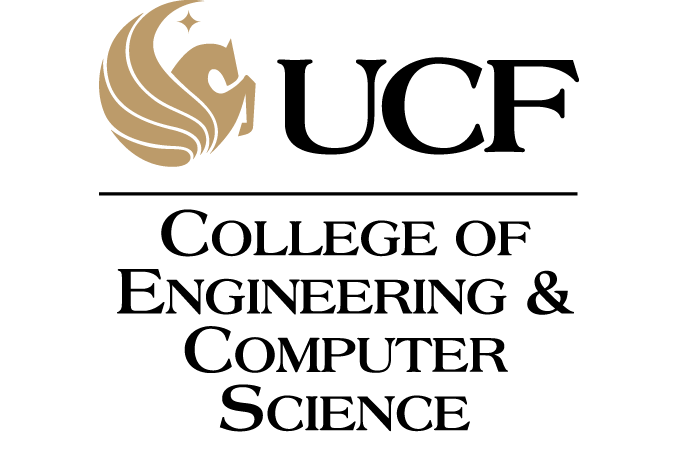
\includegraphics[width=0.45\textwidth]{UCF_logo.png} % Include a department/university logo - this will require the graphicx package
 
%----------------------------------------------------------------------------------------

\vfill % Fill the rest of the page with whitespace
}

\end{titlepage}

% ---------------------------------------------------------
% ---------------------------------------------------------
% ---------------------------------------------------------

% ---------------------------------------------------------
% ---------------------------------------------------------
% ---------------------------------------------------------

\section*{Executive Summary}

\indent\indent Gravity can be a disrupting factor when studying certain phenomena as it may mask the underlying physical processes that govern it. To mitigate the gravitational effects, engineers and scientists have devised controlled microgravity conditions to perform experiments that might otherwise be difficult to perform due to the distortion introduced by gravity. However, due to the high costs of performing microgravity experiments, a large population of scientists are unable to study the effects of weightlessness on certain aspects, whether it be fluid interaction, microbial growth, or material properties.

This report outlines the associated risks, methods/procedures for modeling and analysis, prototyping and testing, and development planning for each major area for the second generation prototype of the low-cost microgravity platform. Each component of the system has been broken down and evaluated for its relation, necessity and benefit to the prototype. All major findings, including changes to the original design, are described.

The first generation prototype as it currently stands consists of a platform and an aeroshell. The platform houses a motor, a reel, brakes, a set of data acquisition instruments, and a systems control unit. On the other hand, the aeroshell houses the payload containing the experiment and an additional set of data acquisition instruments. The aeroshell is attached to the platform via a tether while the platform is in turn attached to a high-altitude balloon that will deliver the system to 30 $km$ in the stratosphere. Consequent to reaching the desired altitude, the aeroshell is released and allowed to drop for a duration of +30 seconds to effectively produce approximately 25 seconds of microgravity. Upon completion of drop, the aeroshell is reeled back and the system readies itself for additional drops.

% ---------------------------------------------------------
% ---------------------------------------------------------
% ---------------------------------------------------------
\newpage

\tableofcontents

% ---------------------------------------------------------
% ---------------------------------------------------------
% ---------------------------------------------------------
\newpage

\listoffigures

% ---------------------------------------------------------
% ---------------------------------------------------------
% ---------------------------------------------------------
\newpage

\listoftables

% ---------------------------------------------------------
% ---------------------------------------------------------
% ---------------------------------------------------------

\include{revision_history}

% ---------------------------------------------------------
% ---------------------------------------------------------
% ---------------------------------------------------------

\newpage
\section*{Terms and Abbreviations}

\begin{table}[H]
\raggedright
\rowcolors{1}{gray!15}{white}
\begin{tabular}{>{\bfseries}L{2cm}L{13.65cm}}
CS  	& Computer Sciences		  							\\
EMA     & Exponential Moving Average                        \\
EOT     & End of Transmission                               \\
FSI  	& Florida Space Institute		  					\\
GPIO    & General Purpose Input/Output                      \\
I$^2$C  & Inter-Integrated Circuit (pronounced I-squared-C) \\
IMU     & Inertial Measurement Unit                         \\
IR      & Infra-red                                         \\
LED     & Light Emitting Diode                              \\
Mbps    & Mega Bits per Second                              \\
ORE     & Optical Rotary Encoder                            \\
PCB     & Printed Circuit Board                             \\
PPR     & Pulses Per Revolution                             \\
PSU     & Power Supply Unit                                 \\
PWM     & Pulse Width Modulation                            \\
RF      & Radio Frequency                                   \\
RPI     & Raspberry Pi                                      \\
SD      & Secured Digital                                   \\
SMA     & Simple Moving Average                             \\
SoC     & System on Chip                                    \\
SOH     & Start of Heading                                  \\
%... 	& ...  												\\
\end{tabular}
\end{table}

\begin{table}[H]
\raggedright
\rowcolors{1}{gray!15}{white}
\begin{tabular}{>{\bfseries}L{2cm}L{13.65cm}}
$\mathbf{a}$		& Acceleration 							\\
$\mathbf{A}$		& Area      							\\
$\mathbf{C_D}$		& Drag Coefficient						\\
$\mathbf{C_g}$		& Center of Gravity						\\
$\mathbf{C_p}$		& Pressure Coefficient					\\
$\mathbf{g}$		& Acceleration Due to Gravity (9.8 m/s)	\\
$\mathbf{\Phi(t)}$	& Heaviside Step Function				\\
$\mathbf{I}$		& Moment of Inertia						\\
%... 	& ...  												\\
\end{tabular}
\end{table}
% ---------------------------------------------------------
% ---------------------------------------------------------
% ---------------------------------------------------------
\newpage
\section{Introduction}

\begin{comment}
Review and update material from the Mid Term Report. This section should concisely address the following issues and point to an appropriate document or Appendix containing detailed information as needed:
•	History behind the project
•	Major end users’ needs and/or problem to be addressed (Present detailed customer requirements in an Appendix.)
•	Justification (benefits) for pursuing the project (worth for solving or improving)
This section also contains a summary of report sections.
\end{comment}

\indent\indent Microgravity is most simply defined defined as a very low acceleration typically compared as a minute relative percentage of Earth's gravity of approximately $9.81 m/s^@$. The prevailing approaches used to achieve microgravity conditions consist of parabolic flights, drop towers, and suborbital flights. Notwithstanding, they all suffer from severe limitations in one form or another, not to mention the exorbitant price tags that are often associated with the operation. For instance, although parabolic flights produce a decent duration of microgravity conditions – up to 25 seconds – they are usually limited to low quality microgravity conditions \cite{Novespace}. Furthermore, the duration of microgravity conditions for experiments performed in drop towers is usually limited by the height of the shaft where the tower is erected. In addition, the time required to evacuate air from the tower to reduce viscous forces is rather long and is a time-consuming process. Lastly, suborbital flights, such as the sounding rocket, can produce 12-13 minutes of microgravity \cite{GAC}. However, it is fairly expensive and campaigns that offer to deliver a payload to a suborbital path are not readily available. Costs to researchers are further inflated when the system requires end-users or research surrogates to manually operate their experimental payloads in person, such as on the International Space Station.

The previously stated limitations are what motivated the design of our system as it aims to reduce, if not eliminate, them. Starting with cost, system components are chosen from mostly off-the-shelf parts, reducing costs required to manufacture highly specialized parts and equipment. In addition, duration limits are also countered by dropping the system from a very high altitude of 30 km. Furthermore, the microgravity quality is theorized to be within the magnitude of $10^{\minus 3}g$. Lastly, the system is designed to be semi-autonomous and capable of carrying out mission critical operations independent of human interaction, allowing for multiple drops within a single flight. No other previously mentioned approach has the combined benefits of the system to be developed.

As noted, our system aims to produce a viable, low cost alternative microgravity solution that can be readily used by scientists aiming to perform experiments in microgravity conditions. Prior to our teams work, a first-generation of previous senior design group at the University of Central Florida produced several innovative concepts that were meant to test the feasibility of such a system. The work of these first-generation teams ranged from addressing subsystem designs to producing a small-scale working prototype. Our second-generation work is largely on the concepts and overall design architecture provided by these earlier teams. Our contributions have been to optimize the design for longer duration flights and produce a working prototype capable of demonstrating those performance requirements. 

This project was created and funded by the Florida Space Institute (FSI) with the guidance of Dr. Adrienne Dove from the University of Central Florida to increase accessibility of testing their microgravity research experiments. However, this project is capable of serving a much larger customer base of research organizations conducting microgravity research experiments such as the National Aeronautics and Space Adminstration (NASA), the European Space Agency (ESA), etc. It could also hold value to commercial entities, such as MadeInSpace or TransAstra, interested in the impacts of microgravity on future technology, including deep space exploration, asteroid mining and the colonization of other planets.

% ---------------------------------------------------------
% ---------------------------------------------------------
% ---------------------------------------------------------

\section{Project Objectives \& Scope}

\begin{comment}
This section contains both long term objectives and the planned semester objectives. Provide a bullet list of the objectives for this semester.  Focus on final outcomes, not intermediate steps. Do not include task assignments in this section. The objectives should be understandable by themselves.  However, you can follow the objectives with a statement of scope to clarify what you planned to do (in scope), and that you planned to not do (out of scope). 
\end{comment}

\indent\indent The ZAP-2 team primary directive to provide a system capable of meeting the customer requirements defined in Appendix \ref{customer_reqs}. To summarize the requirements, we are to produce a dynamic, mechanical system capable of repeatedly providing high-quality ($< 10^{-3}$ g\'s) microgravity conditions for an integrated experimental payload the size of a middeck locker. The system must be able to operate autonomously in stratospheric conditions. To meet these customer requirements we have developed our own series of system level requirements defined in section ~\ref{sys_reqs}. To produce this system and meet these requirements we have developed a list of long-term and semester-long objectives that we've used to guide our efforts. Long-term objectives describe the absolute end goals of this project well beyond the conclusion of our contributions through the senior design course. Semester long goals on the other hand outline the goals that we've worked to achieve throughout and up to the conclusion of this course. They're the goals that our team has worked to meet and deliver. 

\subsection*{Long-term Objectives}

\begin{itemize}
    \item Produce a flight-ready system capable of providing super-high-quality microgravity conditions (on the order of $< 10^{-6}$ g's) for drop durations of up to 25 seconds.
    \item Create a system capable of repeated drops ($> 10$ drops) in a single flight.
    \item Produce a system capable of operating semi-autonomously that allows for user supervision and intervention. 
    \item Fabricate a system capable of operating in stratospheric conditions for hours on end while also being robust enough to endure the dynamic forces throughout a mission while requiring as little maintenance as possible.
\end{itemize}

\subsection*{Semester objectives}

\begin{itemize}
    \item Design and manufacture a potentially flight-ready system capable of providing high-quality microgravity conditions (on the order of $< 10^{-3}$ g's) for drop durations of up to 9 seconds.
    \item Perform critical design analysis on the system concepts to mathematically demonstrate system capabilities.
    \item Identify and utilize affordable, practical manufacturing techniques to create said system and future systems. 
    \item Demonstrate system capabilities by either demonstrating integrated system functionality for up to a 2 second drop or demonstrate individual subsystem capabilities proving their capability to meet their defined performance standards. 
\end{itemize}



% ---------------------------------------------------------
% ---------------------------------------------------------
% ---------------------------------------------------------

\section{Assessment of Relevant Existing Technologies and Standards}

\indent\indent Prior to the conception of our system design our team was tasked with researching existing technologies, systems, hardware, and software that currently provides analogous capabilities or could potentially contribute to our future design. This research is captured in the succeeding documentation. 

Please note, as previously stated, the work of our team is largely based on the architecture provided by the first-generation senior design groups. Therefore, the following details are provided with specific context to the subsystem in which the researched technologies are associated with. 

\subsection{Microgravity Research Platforms}

\indent\indent Today there exists three main methods for achieving microgravity conditions for experimentation, which include drop towers, parabolic flights, and orbital platforms. Drop towers, as their name implies, consist of a chute or tower through which a payload is dropped. The length of microgravity and quality is dependent on the height of the tower and the air resistance the payload experiences. To achieve quality microgravity conditions, drop towers range from a few meters to over one hundred meters and the tower may or may not have air evacuated to create vacuum conditions. Parabolic flights allow experimenters to place their payload into an airplane that then flies through a series of parabolic arcs that create microgravity conditions lasting on the order of tens of seconds. Lastly, orbital platforms such as cubesats or the International Space Station, allow for long term and high-quality microgravity conditions but may be prohibitively costly. Beyond these three main methods also existences unique experimental system, which are often less utilized and include the Japanese Aerospace eXploration Agency's (JAXA) Balloon-based Operation Vehicle (BOV) and quadcopter based paylods. Of all these techniques, our experiment will most closely resemble the JAXA's BOV system.

% ---------------------------------------------------------

\subsubsection{Drop Towers}

\indent\indent A drop tower is, as the name implies, a vertical column inside of which a payload is dropped. During free-fall the payload is expected to experience some level of microgravity conditions. The enhance the quality of microgravity, the vertical column may be evacuated of air to decrease or completely eliminate the drag force the falling payload experiences as it plummets that would otherwise tarnish the quality of microgravity. Drop towers can range from simple open air design being only several meters high to highly complex systems over 100 meters in height.

NASA has two drop towers both located at the Glenn Zero Gravity Research Facility located in Brookpark, Ohio. The largest of the two is a 132 meter tall vacuum chamber tower capable of achieving gravitational accelerations of less than $10^{\minus 5}$ G's for durations of 5.18 second \cite{NASA0G}. It is NASA's premier microgravity drop tower used for studying the effects of microgravity on physical phenomena such as combustion and fluid physics, to develop and demonstrate new technology for future space missions, and to develop and test experiment hardware designed for flight aboard the International Space Station or future spacecraft. The vacuum chamber itself is 142 meters tall and is capable of achieving pressures on the order of $0.05 torr$. Operational procedure begins with a crane lifting the payload to the top of the tower. Air is then evacuated from the chamber. Once the chamber is evacuated the release sequence is initiated by remotely fracturing a specially designed bolt allows the experiment to begin free fall. During the drop the experiment operates autonomously with all experiment power, data acquisition, and control functions located on the vehicle. After falling for approximately 5 seconds the experiment vehicle is stopped in the decelerator cart, located at the bottom of the chamber. The decelerator cart is filled with $3 mm$ diameter expanded polystyrene beads that dissipate the kinetic energy of the $2500 lb$. experiment vehicle. Maximum velocity at the point of deceleration approach $50.5 \sfrac{m}{s}$. The vehicle decelerates from its peak velocity to a standstill in $4.6 m$ of of expanded polystyrene and experiences a peak deceleration rate approaching 65 g's \cite{NASA0G}.

The second drop tower at NASA Glenn Research Center is an open-air 24 meter chute capable of achieving 2.2 seconds of microgravity conditions on the order of $10^{\minus 3}$ G's \cite{JAXALabs}. Because the experimental payload is open to the air, it is also subject to the drag forces due to atmosphere. To minimize these effects researchers employ a drag shield which increase the aerodynamic performance of the payload allowing for diminished drag forces. The payload itself is isolated from the drag shield and falls 19 cm relative to the structure, allowing for optimized microgravity conditions. The payload and shield are then stopped by an airbag deployed at the bottom of the tower \cite{NASADropTower}. 

The Bremen Drop Tower located at The Center of Applied Space Technology and Microgravity (ZARM) in Bremen, Germany, has the world's longest duration microgravity drop tower. The facility features a 120 meter vacuum chamber that can be configured to either drop payloads from the top of the tower or launch them on a catapult system from the bottom of the tower, effectively doubling the duration of microgravity. In the traditional configuration the payload capsule is pulled up to a height of 120 meters to the top of the drop tube and then released. After 4.74 seconds the capsule is decelerated in a unit filled with polystyrene pellets, much like the setup at NASA's Glenn Research Center. Vacuum pumps evacuate the chamber of air to pressure of one ten thousandth of the normal air pressure \cite{ZARM}. In catapult mode a pneumatically driven launch system location at the base of the tower accelerates the capsule to speeds of approximately 168 kilometers per hour in just 0.25 seconds. The velocity and launching force is uniquely calculated for each experiment in order to provide microgravity conditions for up to 9.3 seconds. The same deceleration unit quickly replaces the launch system at the base of the tower ensuring a safe landing for the capsule \cite{ZARM}. 

% ---------------------------------------------------------

\subsubsection{Parabolic Flights}

\indent\indent Parabolic flights, which offer approximately 20-25 seconds of microgravity for 25-30 consecutive parabolas, are currently priced at \$38,500 for a single research team [5]. They offer researchers the ability to test their experiment payloads repeatedly while being present to operate them. Payloads can be either rigidly attached to the plane or be disconnected from their storage unit during flight and free float about the cabin during the periods of microgravity- something unique to parabolic flights. Microgravity is achieved by angling the plane upward, experiencing approximately 1.8 g's,  then smoothly arcing and angling downward, creating the weightless sensation. The actual gravity experienced on parabolic flights is not exactly 0 g, but more accurately $0 \pm 0.01$.

An advantage of parabolic flights is the large number of parabolas flown. Having a large number of parabolas and, consequently, multiple intervals of microgravity, allows researchers to operate there experiments 20-30 times, ensuring more accurate and usable data. During flight, if the experiment becomes non-operational, researchers have the ability to make adjustments to hopefully restore all function and run it during the next parabola. This ties into another advantage of being able to fly onboard with your payload. During other methods of simulating microgravity researchers aren't able to operate their experiment themselves, but rather it needs to be fully automated. A third advantage of parabolic flights is the severity of g-forces experienced by the payloads is a maximum of 2 g's [16]. This is much lower than that of drop towers and suborbital rockets, reducing damage on experiments and offering more design flexibility.

A major disadvantage of parabolic flights is the frequency of which they occur. Currently, ZeroG offers research flights twice per year. These dates are set by the company far in advance, and are subject to change without warning due to weather disturbances or occupied airspace. Another disadvantage is the environment itself- parabolic flights require human interaction with the payloads, increasing the probability for human error. An additional disadvantage is the quality of microgravity. Microgravity is defined as $10^{\minus 9}$ g, but parabolic flights produce approximately 0.01 g's. Additionally, the gravity during those 30 seconds can fluctuate, invalidating the testing done.

% ---------------------------------------------------------

\subsubsection{Orbital/Suborbital Platforms}

\indent\indent For longer durations of microgravity, researchers may look to suborbital and orbital platforms. By definition, a suborbital space flight operates at an altitude higher than $100 Km$ (328,000 ft) above sea level. This altitude is classified as the Kármán line, chosen by the Fédération Aéronautique Internationale; the USAF and the FAA consider a lower altitude of $80.47 Km$ (264,000 ft) as the altitude to qualify as space flight. These options offer cleaner microgravity for longer periods of time, but come with their own unique disadvantages. 

Blue Origin's New Shepard rocket provides approximately 3 minutes worth of clean microgravity and can accommodate payloads up to 50 lbs. They provide vehicle telemetry data, electrical power, cameras, data storage and robust control systems. Blue Origin has flown multiple payloads, including four from UCF's Physics Department (COLLIDE). Virgin Galactic's SpaceshipTwo is still undergoing testing, but has begun reserving spots for research payloads upon completion. SpaceshipTwo will have a 0 g coast phase lasting approximately 4 minutes.

Disadvantages associated with suborbital flights include the severe vibration experienced by experiment payloads, autonomous operation, and varying interface requirements between companies. Vibrational effects are substantial on suborbital flights. SpaceshipTwo expects to experience a maximum of 3.8 g during the boost phase, and a maximum of 6 g during deceleration \cite{L2}. Because of this, research team members must thoroughly prove way in advance via simulations and testing that their payloads are capable of undergoing those forces while maintaining their overall safety levels. Autonomous operation and varying interface requirements are also a disadvantage since payloads need to be manipulated depending on the company they are flying with. Blue Origin offers signal triggering for payloads, as well as a detailed flight profile, while Virgin Galactic requires all triggering to be handled by the researcher teams.

Another major disadvantage of suborbital flights is the infrequency of flight. Because these flights are so costly, they are booked more than a year in advance, require constant communication between the research team and flight company, and a series of paperwork milestones to ensure adequate payload operation and safety. Because of this, flights are often delayed anywhere from 3 months to over a year, depending on the circumstance. Additionally, this may not be a long term solution for researchers since the end goal of these companies is space tourism- experiment payload lockers will be replaced by paying human passengers wanting to become astronauts.

The most well-known orbital platform is the International Space Station (ISS). The ISS was developed by a multitude of nations with the purpose of serving as a shared research platform. The research aboard the ISS is categorized into 3 sections: NASA research, ISS International Laboratories/CASIS, and International Partners. There are 6 phases associated with operating a research payload aboard the station, resulting in a lengthly approval process for all payloads. Today, the only American company to visit the ISS and deliver science payloads is SpaceX via its CRS-8.

While the ISS offers the longest duration of microgravity for research experiments, there are many disadvantages associated with this particular method. First, and most obvious, the selection process is the most selective. While the station houses an extensive number of experiments, the approval process is highly competitive. The cost of sending a research payload to the ISS is also the highest of all methods of testing, requiring funding from NASA grants -or the like- to fund this method of testing. Testing aboard the ISS is the ideal method for a majority of experiments due to the exponentially longer duration of clean microgravity, but is unrealistic for most.

% ---------------------------------------------------------

\subsubsection{JAXA's BOV}

\indent\indent The Japanese Aerospace Exploration Agency’s (JAXA) Institute of Space and Astronautical Science has developed a Balloon-based Operation Vehicle (BOV) that is a link between terrestrial drop towers and the innovative concept our group is working on. The system consists of a high-altitude balloon that lifts a $700 Kg$ payload to approximately $40 Km$ where the BOV is then disconnected and plummets for $20$ to $30 Km$ before deploying parachutes to slow the descent into the ocean \cite{JAXALabs}. The BOV achieves approximately 30 seconds of microgravity as low as 10-4 \cite{JAXALabs}. The BOV itself was designed to be extremely aerodynamic, which resulted in a structure approximating that of a missile or rocket. The experimental payload was then housed inside of this structure where it remained for the entire duration of the flight.

JAXA's BOV was a multi-generational project with each subsequent iteration building on the successes and failures of the previous iteration. The original design incorporated their experimental payload into the BOV by rigidly securing it to the structure. This allowed the payload to remain safely fixed with the caveat that it experienced any vibrational forces or turbulence that the BOV experienced during free-fall. Later generations incorporated one-dimensional and three-dimensional drag-free systems that helped to isolate the payload from the aeroshell and thus insulating it from the forces that would bring the payload out of quality microgravity. The one-dimensional system illustrated in [Fig. ~\ref{fig:JAXABOV.png}] consisted of a simple rail system that allowed the payload to move independently from the BOV in the vertical direction. Cold gas thrusters were also incorporated into the BOV to accelerate the capsule when drag forces began to disturb the BOV/payload displacement. Microgravity conditions lower than $10^{\minus 3}$ g's were achieved for a duration of approximately 30 seconds \cite{JAXAResults}.  The three-dimensional drag-free system, also illustrated in [Fig. ~\ref{fig:JAXABOV.png}] consisted of a spherical payload fixed to the BOV via tethers. The BOV then used 60 cold gas thrusters to keep the outer structure clear of the free-falling payload contained within it. Laser displacement sensors between the two track clearances due to external drag forces. Microgravity conditions up to $10^{\minus 3}$ G's were experienced for durations of only 8 to 10 seconds \cite{JAXAResults}. A tri-axial accelerometer (Silicon Design Inc. Model 2440) was used to track multi-dimensional acceleration to verify and track microgravity conditions. A RHOM-Riken R2-Micro datalogger with a $900 Hz$ sampling rate was used to capture sensor data \cite{JAXALabs}. Temperature and humidity were also captured for climate control to keep the payload within operating conditions.

\begin{figure}[H]
  \centering
  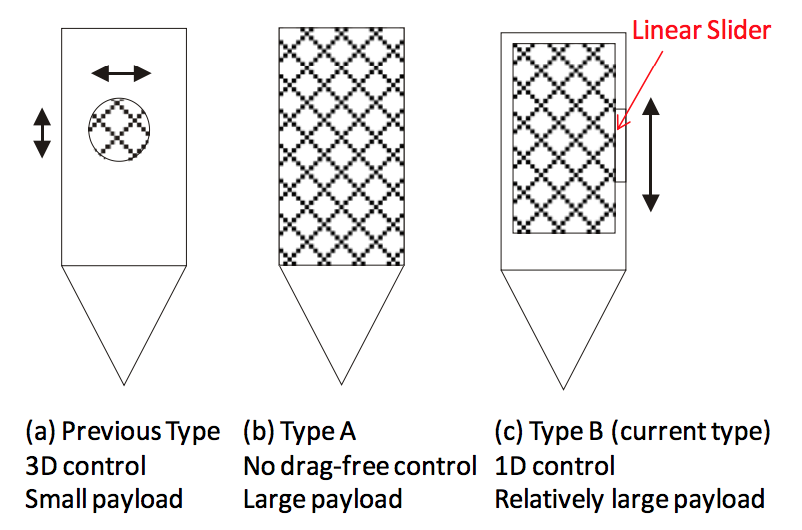
\includegraphics[width=.4\textwidth]{Figures/JAXABOV.png}
  \caption{\label{fig:JAXABOV.png}Drag-free external force isolation systems for payloads in JAXA's BOV vehicle.}
\end{figure}

A major advantage of the one-dimensional drag-free system is that it allowed for a much larger payload and provided almost four times the duration of quality microgravity conditions. The JAXA BOV system most closely approximates our design and provides a wealth of useful information that will influence our design and procedures. Most notably, the vibrational damping/disturbance rejection system, launch procedures, and control technology should all be carefully considered for integration into our design. 



% ---------------------------------------------------------

\subsection{Aeroshell}

\subsubsection{Geometry}

\indent\indent For the aeroshell, the main goal of the geometry is to decrease the amount of drag force and initial pressure while dropping through the stratosphere to achieve microgravity. A symmetrical airfoil is chosen because it will not produce a significant amount of lift and it decreases the drag coefficient during the drop. The specific symmetrical airfoil chosen is a hydrofoil, which has the main purpose of lifting a boat's hull above water. The hydrofoil decreases drag and also gains speed on its travel path. There are many other airfoils that are candidates, such as, aerobatic and NACA airfoils. The hydrofoil is not a conventional airfoil that can be seen on a general aircraft wing or tail. Hydrofoils tend to have a sharper trailing edges, which is similar to subsonic flight airfoils.

Optimization of airfoils to decrease drag is the current technology to produce better and more efficient airfoils for various uses. These airfoil uses range from turbines, turbofans, propellers, and airliners. The optimization process tends to yield results for high lift to drag ratio. The process can use a Matlab code and call another program within the code to retrieve different airfoils and "mutate" the airfoils through each iteration. The called program tends to be XFoil, which is a program for design and analysis of subsonic isolated airfoils. The different methods used within the optimization codes to parameterize the airfoils are PARSEC, CST, and a variant of Karman-Trefftz. For the purpose of this chosen symmetric airfoil, the desire is to have a low drag and to minimize any lift that would occur during flight. There are little to no codes created for symmetric airfoils with the main purpose of decreasing the drag coefficient. However, a code by Zheng Wang using Genetic Algorithm optimizes symmetrical airfoils \cite{optimize}. This optmization code also uses XFoil as a program to create "mutated" airfoils and to iterate the airfoils until the optimizer has converged.

% ---------------------------------------------------------

\subsubsection{Payload}

\indent\indent To ensure the system is versatile enough to accommodate a wide variety of microgravity payloads, the internal structure of the aeroshell will be designed to the specifications of a middeck locker. The three designs considered for housing the payload were a static attachment, an linear rail system, and a 3 dimentional isolation system. The static attachment would be the simplest to implement but the most likely to lower the quality of microgravity for the payload. The linear rail would improve the quality of microgravity considerably over a static attachment, but would also greatly increase complexity and modes of failure. A 3 dimentional isolation system, similar to that employed by JAXA \cite{JAXALabs} would allow for the greatest fidelity of microgravity but also the greatest complexity. 

The standard middeck locker was the payload size specification requested by the intended user of the microgravity platform. The aeroshell will use a standard middeck locker to contain the payloads, and mount any payload hardware to a standard adaptor plate. This simplifies the design requirements of the aeroshell internal hardware because whichever isolation technique is used, the payload will always be a standard size and shape.

The choice of mounting and isolation drives many subsequent design requirements. A simple attachment would minimize the greatest diameter of the aeroshell. The aeroshell would need only to fit the width of the middeck locker at the top and bottom panels. A linear rail would increase the aeroshell diameter because the aeroshell would need to accommidate the width of the middick locker at both the top and the bottom of the rail system. To maintain the chosen aeroshell shape, the length and diameter of the aeroshell would increase significantly. This holds true for the 3 dimentional isolation system as well. The simple attachment is the recommended method for the current iteration of the project.

The two more complicated options also introduce the need of a control system. To ensure the benefit of the linear rail is applied to every drop test, the aeroshell would need a method to raise the payload within the aeroshell, hold the payload at the top of the rail, but still allow the payload to slide along the rail unimpeded. The recommended method to achieve this is to raise the payload with a pushing linear actuator until the payload reaches the top, engage an electromagnet at the top of the rail to hold the payload in place while the linear actuator retracts, then simultaneously release the electormagnet and the aeroshell as a whole. This system is strongly recommended for future iterations of this project, but ultimately out of the scope of the current iteration of the aeroshell.

% ---------------------------------------------------------

\subsubsection{Latch}

\indent\indent Since the aeroshell is to be manufactured in halves it warrants a way to align and fix them together. Many candidates were considered such as case latches (used in heavy duty road cases), snap latches (used in many flexible case enclosures), and hook and eye latches. Ultimately, it was decided to incorporate roto-lock coffin latches into the design for their strength, holding capacity ($750 kg$ each), and ease of use. With one hex key, the coffin latch can be engaged or disengaged to join or release the two halves in seconds; however, since it is originally designed as a “latching biscuit joint” an additional aluminum part will need to be machined and bonded to the aeroshell to make use of it as an internal latch. Also, additional carbon fiber layers can be applied during fabrication to thicken and increase strength of the attachment points to avoid pull-through and shear-out failure conditions at the bolt interface. Finally, if necessary, a small scoop could be installed over the bolts to help alleviate the drag of the exposed metal. Although the aeroshell will be directly fastened to the internal structure in separate locations, having the coffin latch will speed up assembly and provide a redundant system to ensure the shell stays closed and aligned.

% ---------------------------------------------------------

\subsection{TUMBR}

\subsubsection{Tether}

\indent\indent The material of the tether must be lightweight, durable, and resistant to atmospheric conditions that may weaken the functionality. The best solution found for this material is Spectra, developed by Honeywell. The material is known to be one of the world’s strongest and lightest man-made fibers, and has been implemented by the Department of Defense (DOD) for military and police applications. Spectra is fifteen times stronger than steel, more durable than polyester, and resists corrosion, chemicals, and abrasion, making it an ideal choice for repeated impact and atmospheric conditions. The disadvantages found with this material are the high cost and lead time. The material chosen by the previous team for the scaled model, however, was Kevlar, due to its high strength, low creep, good temperature performance, and low stretch \cite{trt}. For this iteration of the project we will be moving forward with Spectra by Honeywell and proceeding with a 9 second drop. A major constraint of the tether will be the diameter and weight, which was allocated to a max of $5 mm$ and $100 Kg$ by the previous team. By scaling up the project to perform a 9 second drop, the length of tether needed will be approximately 600 km.

% ---------------------------------------------------------

\subsubsection{Unit}

\indent\indent The platform structure will house the tether/reel and tether guide, braking system, and dual motors. The previous iteration of the project constructed the platform frame from 80/20 Aluminum. This material is commonly used in engineering applications due to the low cost, high strength to weight ratio, availability, and ease of machining. 80/20 is 2x stronger than steel and approximately one third the weight, offering a unique opportunity for frame applications. This material is also much less corrosive than comparable metals, and keeps its shape when exposed to temperature changes- unlike steel. 80/20 also comes in a T-slot design, which makes adjusting attachment points and altering designs much more feasible since those attachments are not permanent. As a result, these pieces can be re-purposed at the conclusion of a project rather than discarded- reducing overall costs. 

% ---------------------------------------------------------

\subsubsection{Motor}

\indent\indent The motors used in the prototype for both applications were AmpFlow E30-150 24-volt DC motor, which could operate between 12-36 volts, have $5 Nm$ of torque, produce around $750 W$, and can produce maximum RPM of $8700 RPM$. Calculations showed that $8.4 Nm$ of torque would be required to lift the aeroshell, however the motor on the system for reeling the payload back onto the spool can only produce $5 Nm$ of torque. Through a gear reduction of 9/32, a max torque of $17.78 Nm$ would be produced by the motor and would meet the required torque to raise the payload.

Three types of electric motors were considered for the system: AC, brushed DC and brushless DC. AC motors are powered by an alternating current that runs through a stator, producing a magnetic field. The previous team opted not to use AC motors due to their significantly higher cost and slightly increased performance. DC motors are powered via a direct current and are much more feasible at higher altitudes. A set of magnets are positioned within the stator and the armature has wire wrapped around an iron core. Depending on whether the motor is brushed or brushless determines the operation; brushless motors use a controller to activate/deactivate each coil. Brushed motors transmit power through brushes to energize the wires at specific times. Brushed DC motors require more maintenance and have a shorter life than brushless DC motors, but offer reduced initial costs and better control.

% ---------------------------------------------------------

\subsubsection{Brake Systems}

\indent\indent Braking systems can be complex to manufacture, so the previous team decided it was best to design the brake system with items which could easily be obtained from off-shelf items and replaced easily if necessary. A simple friction-based caliper and rotor setup was designed to attach to the platform and the shaft of the system. Friction based braking is a very reliable and predictable way to slow down an object, with the only major downfall being the replacement of the friction material (brake pads or rotor). The caliper and rotor on the first generation prototype were both fashioned from a Honda Fit and calculations proved that a deceleration was more than enough to bring the aeroshell to a safe halt. A linear actuator was connected to the master cylinder of the braking system so the controls and instrumentation team could precisely apply pressure when coupled with a microcontroller.

The braking system on the prototype is currently non-functional due a tilt in the rotor and uneven caliper mounting when assembled. The slight tilt in the rotor coupled with an uneven caliper mount produces a non-uniform deceleration with heavily increased frictional forces. The increased friction caused by this manufacturing error prevented the previous team from full integration testing.

The previous team used an iron rotor fashioned from a Honda Fit for their frictional braking system. The rotor on the system will be rotating approximately upwards of 5,000 revolutions per meter (RPM) for a nine second drop which leads to a large heat flux and large shear force when braking is applied. Iron rotors are heavy and known to deform and warp at high temperatures and loads. These are very undesirable traits when weight, reliability, and repeatability are three important factors dealing with this project. Carbon-ceramic brakes are used in high end cars because of the great response in both wet and dry conditions, the high durability, the low weight, resistance to corrosion and are characterized by having an extremely low deformation under high temperatures.
% * <jkirschbaum1992@gmail.com> 2018-04-16T00:41:11.304Z:
% 
% " Because of these inherent traits of iron high performance cars turn their eyes to another material which will perform much better under stressful environments."    
% 
% Wat?
% 
% ^.

Future modifications made to the braking system will include the addition of an electromagnetic braking system. The two systems will function as a combined braking system- the electromagnetic initiating first to slow the shaft to an optimal angular velocity, at which point the frictional system will begin operating to slow the speed to zero. Electromagnetic braking systems are currently used in high velocity applications, such as trains and roller coasters. A major disadvantage is the proportional braking force and velocity, meaning the system loses efficiency as the velocity decreases. For this reason a frictional system will remain a part of the design. The decreased velocity when the frictional system begins will extend the life of both the brake pad and rotor.

% ---------------------------------------------------------

\subsubsection{Reel}

\indent\indent The reel has four main components: the shaft, tether walls, frame, and bearings. The shaft, tether walls and frame were constructed from steel, while the bearings were made from stainless steel. The frame was fabricated with 2” square 80/20 bars welded at the corners with an x-brace design at both ends to maximize strength and minimize weight.  In the center, a cylindrical shaft holds two 10” diameter discs which acts as a housing to hold the tether in place on the shaft. To help release the tether from the reel, two disks were fabricated to clamp the tether and pull it off the reel at $2107 RPM$.

A major consideration for the reel includes a tether guide to ensure no additional forces are acting on the tether and reduce overall vibration on the aeroshell. By adding this mechanism to the platform, the tether will cleanly unroll and respool each drop without tangling or knotting. Previous designs were constructed for a functioning tether guide, but their interface with the overall platform was not ideal. Current mechanisms exist and will be implemented in the design.

% ---------------------------------------------------------

\subsection{Controls \& Instrumentation}

\indent\indent The development of the controls and instrumentation module of the second generation prototype was distributed amongst the MA team and the CS team in order to allow the MA team to focus on developing the mechanical and structural components of the system. However, the MA team was given the task of choosing the appropriate sensors and developing the required code to interface them with the controls system that is to be provided by the CS team.
Certain requirements need to be met for the the successful trial runs and meaningful data collection.

\begin{enumerate}
\item Controls unit must be able to interface with all the sensors on board.
\item Sensors need to relay data back to the controls unit for logging and data storage.
\item Controls unit and sensors must both be able to operate under harsh environmental conditions.
\item A proper calibration routine must be performed to reduce the effects of ambient noise.
\item Sensors must be repeatable and of high fidelity.
\item Must be cost-effective in order to fulfill the imperative of this mission.
\item Must be feasible to integrate within the system
\end{enumerate}

The conceptualized controls and instrumentation module layout as envisioned by the CS team is presented in [Fig. 3].

\subsubsection{IMU}

\indent\indent The IMU must be able to record the acceleration of the system as it is being dropped. In order to gather high quality data, the signal must have a low noise density, this can be achieved by actively filtering the data software wise in conjunction with the addition of an appropriate capacitor near the signal line of the breakout board of the sensor. Furthermore, the IMU must be able to record accelerations of at least $10^{−3} m/s^{2}$ for the data to be meaningful. Being able to achieve such values heavily rely on the resolution and sensitivity of the sensor, and as such, the IMU must have a resolution and sensitivity that allows it to measure and record accelerations in the range of $10^{−3} m/s^{2}$.

\subsubsection{Temperature Sensors}
\indent\indent As with the IMU, the temperature sensor must be able to monitor and record the experimental environment conditions and possibly monitor the system’s condition. Such data is vital for the experimenter as will as for the operation of the system. For instance, a temperature sensor could be employed to monitor the motor’s temperature. In case the motor overheats for any reason, the temperature sensor could signal the control unit to halt the next drop until the motor cools down.

\subsubsection{RPM Measurement Device}

\indent\indent The monitoring of the RPM at which the tether is being ejected is one of the most important parts of the experiment as the ability to achieve microgravity is dependent on the team’s ability to reduce all the forces acting on the aeroshell. The role of the RPM measurement device is to signal the motor to run at a higher speed such that it unwinds tether from the spool at a slightly faster rate than that of which the tether is being ejected from the system. For the RPM measurement device to be effective, it must be able to read and register RPMs of +5,000 as per the preliminary calculations. To that end, two types of measurement devices can be used; a tachometer or a rotary encoder. However, it must be noted that for the purposes of prototype validation a rotary encoder is to be used while a tachometer is to be used for the full-scale system for reasons that are discussed in section ***5.5.3***.

\subsubsection{Controls Unit}

\indent\indent The controls unit can be thought of as the central hub of the system where everything has to go through and where all the commands are issued and executed. In order to fulfill this purpose, the controls unit must have ample GPIO pins to interface all the sensors and peripherals. Moreover, the controls unit must have adequate processing power to perform all the calculations and data storage operations in real-time.

\indent Previous teams opted for the use of the Arduino MCU in parallel to a RPi running the Raspbian Jessie OS. This added a layer of complexity to the controls and instrumentation module as data had to go through two hops before reaching its final destination. This can be mitigated by the use of a RPi running a minimal OS known as DietPi that is light on resources, leaving said resources available for the interaction between the RPi and the remainder of the system [24]. Additionally, the RPi can be overclocked allowing for a higher frequency effectively reducing lag between the moment at which data is received, processed, and an appropriate command is issued.

\subsubsection{Programming Language}

\indent\indent A programming language must be used to produce a set of instructions that can be used to produce various kinds of output and implement specific algorithms. The choice of an appropriate language is important as it determines whether the controls and instrumentation module will operate in real-time or not.

\indent Two classes of programming languages exist; interpreted and compiled languages. Interpreted languages, as the name implies, are interpreted at run-time and everything is processed as the interpreter reads a line of code. On the other hand, compiled languages assemble the code prior to execution and converts it to a lower-level form in which the program can be executed, reducing a level of abstraction found in interpreted languages.

\indent Previous teams had used a mix of both languages on the first generation prototype. As an example, all the MCU’s were programmed using C/C++, a compiled language, and all the RPi’s were programmed using Python, an interpreted language. For the sake of continuous improvement, the second generation will be using C/C++ for all programming purposes as it offers unparalleled execution speeds when compared to an interpreted language such as Python, allowing for near real-time operation.

\subsection{Power Supply Unit}

\indent\indent Lastly, no previous intensive work was aimed at the power supply and distribution units by the previous teams. Given that it is a vital part for the operation of the entire system, the second generation prototype would be giving much needed attention to the power supply and distribution unit.

\indent Various types of power supply solutions exist on the market. However, reducing the number of alternatives was relatively easy as batteries that contained toxic chemicals, such as NiCd batteries, were immediately dropped from consideration. Nonetheless, out of the remaining alternatives, the high current type Li-Ion/Li-Poly batteries were chosen due to the amount of power per unit weight that each cell in the battery can hold.

\indent As for power distribution, the team has not settled on any specific approach as the system design parameters were constantly changing throughout the semester and gauging the system’s requirements and potential power distribution scheme was deemed as future work.

% ---------------------------------------------------------
% ---------------------------------------------------------
% ---------------------------------------------------------

\section{Professional and Societal Considerations}

\indent\indent The ZAP-2 brings a novel and cost effective approach to the way researchers and scientists can get access to high quality microgravity conditions for various types of experimentation. Currently, the cost for this type of enabling technology ranges from tens of thousands to hundreds of thousands and even millions of dollars. If a disrupting new technology such as this one were to enter the marketplace it would surely allow for more scientists and researchers to have access to high quality microgravity conditions, thus creating the opportunity for scientific studies to flourish. With more affordable access to this type of research, scientists would have more money to spend on opening up opportunities for undergraduate and graduate students to join these projects. A saving in funding would also create the opportunities for more travel to conferences, new laboratory equipment, and so on. It stands to reason that if the ZAP-2 were brought to full development, the impact to the field of microgravity research would become available to more people to participate in than ever before.

% ---------------------------------------------------------
% ---------------------------------------------------------
% ---------------------------------------------------------

\section{\label{sys_reqs}System Requirements and Design Constraints}

\indent\indent The design of our group's system was largely based around the concept of the first iteration design carried out by The Green Team. This allowed key components and key functions that are necessary to achieve the project goals and requirements to be identified and characterized. While many of these components have been studied in further detail for optimization and upgrade the key functional requirements remain the same.

\indent\indent Our design features two macrostructures and are detailed further in the System Concept Development section (\ref{sys_concept_dev}) of the report. The TUMBR is the structure that is fixed to the stratospheric balloon and houses the tether brake and reel system, the motors, and a variety of onboard computers and sensors. The aeroshell is the structure that houses the payload, is attached to the TUMBR via the tether, and is dropped in order to experience microgravity conditions. Subsystems are first identified by the macrostructure that they belong to, either the aeroshell or TUMBR. System requirements identified for each of these assumed subsystems and then presented. Each system requirement is then traced to the project goals and requirements from which it was derived.

\subsection{Aeroshell}

\indent\indent The aeroshell is the part of the system that houses the payload. The payload will contain a mid-deck locker, which is where the actual microgravity experiment will be placed. The aeorshell willbe attached to the TUMBR system via tether and will also house all the corresponding electronics.

\subsubsection{Aeroshell Controls and Electronics}

\subsubsection*{Acceleration Log}
\indent\indent The aeroshell must record, transmit, and store the 3-axis reduced acceleration experienced by the module with precision of up to $10^{\minus3}$ g’s. Traced to: 2.1 Microgravity Conditions

\subsubsection*{Climate Control}
\indent\indent It must record climate data including temperature, pressure, and humidity as well as temperature of critical components and provide climate control solutions to keep components within operating conditions. Traced to: 2.2 Environmental Considerations

\subsubsection*{Filters}
\indent\indent If possible, filters or other noise-canceling devices must operate to ensure clean acceleration readings. Traced to: 2.1 Microgravity Conditions

\subsubsection*{Communication}
\indent\indent The system must be capable of communicating with a the TUMBR. Communication is defined as the transmission of relevant experimental data. Traced to: 2.8 Safety

\subsubsection*{Data Storage}
\indent\indent The system must be able to continue to store data when it loses wireless connection to the TUMBR. Traced to: 2.1 Microgavity Conditions

\subsubsection*{Autonomy}
\indent\indent The system must be capable of autonomous control but allow for user supervision. Traced to: 2.3 Reusability and Repeatability

\subsubsection*{Velocity Log}
\indent\indent The velocity of the aeroshell and the tether must be monitored and used as feedback for potential motor and brake control. Traced to: 2.1 Microgravity Conditions

\subsubsection*{Data Speed}
\indent\indent Control systems (computers, controllers, and sensors) must be capable of sensing, recording, and transmitting data fast enough to counteract disturbances and maintain microgravity conditions. Traced to: 2.1 Microgravity Conditions

\subsubsection*{Status Check}
\indent\indent The TUMBR must perform a status check and receive the status check from the aeroshell prior to each drop. Traced to: 2.8 Safety

\subsubsection*{Multiple Data Logs}
\indent\indent The system should have multiple redundant data logs. Traced to: 2.8 Safety

\subsubsection*{Redundancy}
\indent\indent It should allow for certain instruments to cross-talk, redundant sensors. Traced to: 2.8 Safety 

\subsubsection{Aeroshell Structure}

\subsubsection*{Geometry}
\indent\indent The aeroshell geometry must be able to snugly fit all the components of system. This includes ,but is not limited to, the payload, the controls and electronics, the power supply, and the internal structure. The aeroshell must meet the specific requirement of having a low drag coefficient. The team decided that the coefficient of drag must be less than 0.5 in order to have the most effective aeroshell. The geometry of the aeroshell is what will dictate the drag coefficient it will have; thus the geometry must be carefully selected to ensure the best one is chosen. The geometry must be able to be shaped easily without compromising machinability and strength. The geometry must be designed to experience a nominal 5 g’s, and a maximum of 10 g’s, of vertical acceleration. This vertical acceleration may be experienced during the deceleration phase of the drop. The geometry of the aeroshell must provide the team with easy access to the inside were the integration of the payload, internal structure, electronics, and other systems will be contained. The hardware that holds the aeroshell together must no increase the drag by more than 10 percent of the idealized case. This means that the latches chosen to close the aeroshell must maintain the aerodynamic integrity of the system. The aeroshell must consider accommodating future propulsion design integrations. Also, the aeroshell must connect to the tether in a secure way to ensure the survival of the maximum forces felt during experimentation. Traced to: 2.10 Strength and Durability


\subsubsection*{Manufacturability}
\indent\indent The design of the aeroshell must be manufacturable i.e. capable of being fabricated from student-accessible resources. The method of manufacturability must be one that can be reproduced by future iterations of the project. It must be manufactured in a way that does not compromise the aerodynamic effectiveness of the chosen airfoil. Another important requirement is that it must be firmly held together so that it does not come apart while it is performing a drop or reeling itself back up. All these factors must be taken into account when choosing the most feasible method of manufacturing the aeroshell. Traced to: 2.3 Reusable and Repeatability

\subsubsection*{Material Selection}
\indent\indent The aeroshell will be dropped from $100,000 ft$ above sea level, so it should be able to withstand the harsh environmental conditions from the stratosphere.  Some of the minimum conditions that it must endure are a temperature of $-46\degree C$ ($227 K$) and a pressure of $1.12 kPa$. The aeroshell should also have a vibrational damping system capable of resisting any vibration felt due to turbulence as well as vibrations from the reeling tether. The material selected must be sturdy enough to maintain the aeroshell as stable as possible during the drops, while not compromising the weight. The material must be light weight, in order to not exceed the mass budget of $400 Kg$. The structural material must be able to be easily shaped without compromising machinability and strength. Traced to: 2.2 Environmental Considerations

\subsubsection*{Aerodynamics and Stability}
\indent\indent The aeroshell must have a stable and efficient design to enable microgravity conditions for payloads. This includes but is not limited to: resistance to drag, resistance to torques and lateral forces, and induced vibrations leading to accelerations that take the payload out of microgravity conditions ($10^{\minus2}$ g). The coefficient of drag must be less than 0.5. Traced to: 2.1 Microgravity Conditions. 

\subsubsection*{Strength}
\indent\indent Must be strong enough to endure associated forced with multiple high-speed drops and decelerations of up to 10 g’s (5 g’s) without plastic deformation. Traced to: 2.10 Strength and Durability

\subsubsection*{Propulsion Integration}
\indent\indent The design must consider accommodating future propulsion system integrations. Traced to: 2.1 Microgravity Conditions

\subsubsection*{Tether Connection}
\indent\indent The aeroshell must connect to the tether in a safe and secure way as to ensure survival through maximum forces. Strength and Durability. The connection to the tether must also be strong enough to support any crosswinds the aeroshell may encounter on its way down. It must be able to latch on and lock itself so it will not have any possibility of opening and disconnecting itself from the tether during a drop. The tether connection must also not add much weight to the overall aeroshell system, as well as maintain its strength and durability during repeated drops.Traced to: 2.8 Safety

\subsubsection{Aeroshell Power Supply}

\subsubsection*{One Mission Supply}
\indent\indent A power supply capable of supplying power to maintain all systems for the duration of at least one mission shall be implemented. Traced to: 2.3 Reusability and Repeatability

\subsubsection*{Mass}
\indent\indent Must have an optimized mass and size. Traced to: 2.4 Mass Budget

\subsubsection*{Safety}
\indent\indent Must be safe, not explode, and must be ensured with a reasonable degree of confidence not to be a point of failure with potential to kill a mission. Traced to: 2.8 Safety

\subsubsection{Internal Structure}

\subsubsection*{Geometry}
\indent\indent The internal structure must provide a rigid framework or scaffolding that will host the various aeroshell systems while remaining fixed to the aeroshell structure. It must be made of a material that is strong and durable, but does not cause the aeroshell system to exceed the weight limit. It must integrate the tether connection system so that the tether has a secure attachment point to avoid failure during drops. The main objective of the internal structure is to have a housing for the payload, electronics, and power supply. This is essential for the experiment since it is important to have all the items inside the aeroshell securely fastened during drops. The internal structure must account for the size of the middeck locker, which is what the payload consist of. The internal structure must also be able to withstand any vibrations felt from the external forces, as well as the deceleration forces. The internal structure must maintain its stability in order for the microgravity experiment to run smoothly and error free. Traced to: 2.10 Strength and Durability


\subsubsection*{Strength}
\indent\indent Must be strong enough to endure associated forced with multiple high-speed drops and decelerations of up to 10 g’s (5 g’s) without plastic deformation. Traced to: 2.10 Strength and Durability

\subsubsection{Payload and Integration}

\subsubsection*{Payload Accommodation}
\indent\indent The aeroshell must be able to accommodate a payload with the dimensions of a middeck locker (scaled-down middeck locker) used on Space Shuttle. The middeck locker is the specific area were the experiment will be housed. This was chosen by the customers, so it is critical that the team successfully incorporates the middeck locker into the design. Traced to: 2.12 Payload


\subsection{TUMBR}

The TUMBR system (Tether, Unit, Motors, Brakes, and Reel) houses all the key components that enable the aeroshell to achieve microgravity conditions. As expressed in the acronym, the TUMBR consists of the tether, platform unit, motors, brakes, and reel system. Also onboard the TUMBR are the computers and electronics that command the individual components to work in tandem with each other to achieve the desired performance. 

\subsubsection{Braking}

\subsubsection*{Max Deceleration}
\indent\indent The braking system must slow the aeroshell in a way that it experiences no more than an acceleration of 5 g’s. Traced to: 2.10 Strength and Durability

\subsubsection*{Heat Loss}
\indent\indent The braking system must be designed in a way to minimize heat loss or provide a means for heat to be captured and moved. Traced to: 2.5 Maintenance

\subsubsection*{Fail-Safe}
\indent\indent There must be a fail-safe and/or back-up break integrated into the system. If this is impractical then operational safety procedures must be put in place. Traced to: 2.8 Safety

\subsubsection*{Feedback Control}
\indent\indent The braking system should use aeroshell and/or acceleration and/or velocity data as feedback for ramped and controlled braking. Traced to: 2.10 Strength and Durability

\subsubsection*{Jerk}
\indent\indent The braking system should operate as to minimize the jerk experienced by the aeroshell. Traced to: 2.10 Strength and Durability

\subsubsection*{Stationing}
\indent\indent The braking system must be capable of holding aeroshell between flights and during launch and descent. Traced to: Reusability and Repeatability

\subsubsection{Reel Motor}

\subsubsection*{Reeling Duration}
\indent\indent The reel motor must be able to reel in the aeroshell within one hour. Traced to: 2.3 Reusability and Repeatability

\subsubsection*{Repeatability}
\indent\indent The motor must be capable of performing this task for as many drops as are scheduled within the mission. Traced to: 2.3 Reusability and Repeatability 

\subsubsection{Release Motor}

\subsubsection*{Release Velocity}
\indent\indent The release motor must be able to unspool the tether at a rate equal to or slightly greater than the downward velocity of the aeroshell as it drops. This is to ensure that there is no tension in the tether. Traced to: 2.1 Microgravity Conditions

\subsubsection*{Feedback}
\indent\indent The release motor system should use aeroshell and/or acceleration and/or velocity data as feedback for controlled tether release. Traced to: 2.1 Microgravity Conditions

\subsubsection*{No-slip Condition}
\indent\indent Tether release needs to ensure a no-slip condition. Traced to: Microgravity Conditions

\subsubsection{Tether}

\subsubsection*{Connection Points}
\indent\indent Tether must securely connect to the aeroshell at one end and the reel on the TUMBR on the other, where it is reeled up for release and subsequent reeling. Traced to: 2.10 Strength and Durability

\subsubsection*{Tether Strength}
\indent\indent Tether must be strong enough to support the aeroshell for entire length of mission, which include the force experienced during aeroshell deceleration. Traced to: 2.10 Strength and Durability

\subsubsection*{Tether Diameter}
\indent\indent The tether diameter should be minimized to maximize length on spool. Traced to: 2.4 Mass Budget

\subsubsection*{Length}
\indent\indent Tether should be long enough to accommodate a maximum 25 second drop (2 – 9 second drop) followed by a 5 G deceleration period. Traced to: 2.1 Microgravity Conditions

\subsubsection{Tether Guide}

\subsubsection*{Clean Reel}
\indent\indent Spooling systems must, by design, be capable of cleanly reeling in the tether after every drop to ensure no tangling or knotting of the tether. Traced to: Reusability and Repeatability

\subsubsection{TUMBR Controls and Electronics}

\subsubsection*{Communication}
\indent\indent The system must be capable of communicating with the aeroshell and a ground station. Communication is defined as the transmission of relevant experimental data and controls sent from ground-station operators. Traced to: 2.8 Safety

\subsubsection*{Autonomy}
\indent\indent The system must be capable of autonomous control but allow for user supervision. Traced to: 2.8 Safety

\subsubsection*{Velocity/Acceleration Feedback}
\indent\indent The velocity and displacement of the aeroshell and the tether must be monitored and used as feedback for motor control. Traced to: 2.1 Microgravity Conditions

\subsubsection*{Disturbance Rejection}
\indent\indent Control systems (computers, controllers, and sensors) must be capable of sensing, recording, and transmitting data fast enough to counteract disturbances and maintain microgravity conditions. Traced to: 2.1 Microgravity Conditions

\subsubsection*{Status Check}
\indent\indent The TUMBR must perform a status check and receive the status check from the aeroshell prior to each drop. Traced to: 2.8 Safety

\subsubsection*{Redundancy}
\indent\indent The system should have multiple data logs and it should allow for certain instruments to cross-talk, redundant sensors. Traced to: 2.8

\subsubsection{TUBMR Power Supply}

\subsubsection*{Total Power}
\indent\indent The power supply system must provide enough power for all motor control (unspooling, reeling in), braking, and electronics. Traced to: 2.3 Reusability and Repeatability

\subsubsection*{Power Duration}
\indent\indent The power supply must provide adequate power for the entire mission. Traced to: 2.3 Reusability and Repeatability

\subsubsection{TUBMR Structure and Platform}
 
\subsubsection*{Mass and Strength}
\indent\indent The structure or TUMBR housing should provide a strong rigid platform to affix the listed systems to without risk of structural failure all while fitting into the overall mass budget i.e. mass should be optimized. Traced to: 2.10 Strength and Durability

\subsubsection*{No Flexing}
\indent\indent The reel should be strong enough as not to flex, deform, or fail at any point during a mission. Traced to: 2.10 Strength and Durability


\begin{comment}
\indent\indent Revise and update the corresponding section from your mid-term report. For any requirement or constraint derived from a stand or regulation, make sure to cite it. 
\indent\indent Present the key functions and/or features of the system (product, or process/services) you are designing.  Describe the theory of operation, benchmarking analysis and any industry and/or de facto standards that are relevant to your project. Present a summary of the key system requirements, critical parameters and specifications here.  Provide detailed requirements and specifications in an Appendix.
\end{comment}

% ---------------------------------------------------------
% ---------------------------------------------------------
% ---------------------------------------------------------

\section{\label{sys_concept_dev}System Concept Development}

\begin{comment}

To Do: Present the system concept that the team ultimately developed.  Where appropriate, refer to previous final report(s). Help the reader visualize the system concept by using appropriate drawings/diagrams, such as sketches, system schematics, circuit diagrams, and UML diagrams. Describe the significant criteria that lead to concept selection, alternate concepts that were considered, and design trade-offs.  For the remaining concepts considered, provide appropriate pointers, such as the section in your Mid Term Report. 

\end{comment}

\subsection{The ZAP-2 System}

\indent\indent The Zero-g Aero-Drop Project 2 (ZAP-2) system largely builds on the successes and best practices of lasts year's senior design groups. A majority of the conceptual design was retained from the first iteration. However, comprehensive and thorough analyses of subsystems and their components have allowed us to refine the architecture of the system and introduce design optimizations where it was possible. The system design has also been scaled up to allow for longer duration drops on the order of 2 to 9 seconds.

The ZAP-2 System consists of two macrostructures: the aeroshell and TUMBR. Interfacing between the two macrostructures is the tether, which firmly anchors the aeroshell to the TUMBR. Housed inside of the aeroshell is the internal structure or skeleton, which itself houses the mission payload and provides a mounting point for the tether connector and the electronics, and controls system. The TUMBR provides a rigid platform for the tether/reel, brakes, motors, and electronics and controls package to be fixed to. Each of these systems and subsystems will be detailed further in the succeeding subsections. A systems diagram created in the CAMEO System Modeler software package is shown in [Fig. \ref{fig:CAMEO}]. 

\begin{figure}[ht]
  \centering
  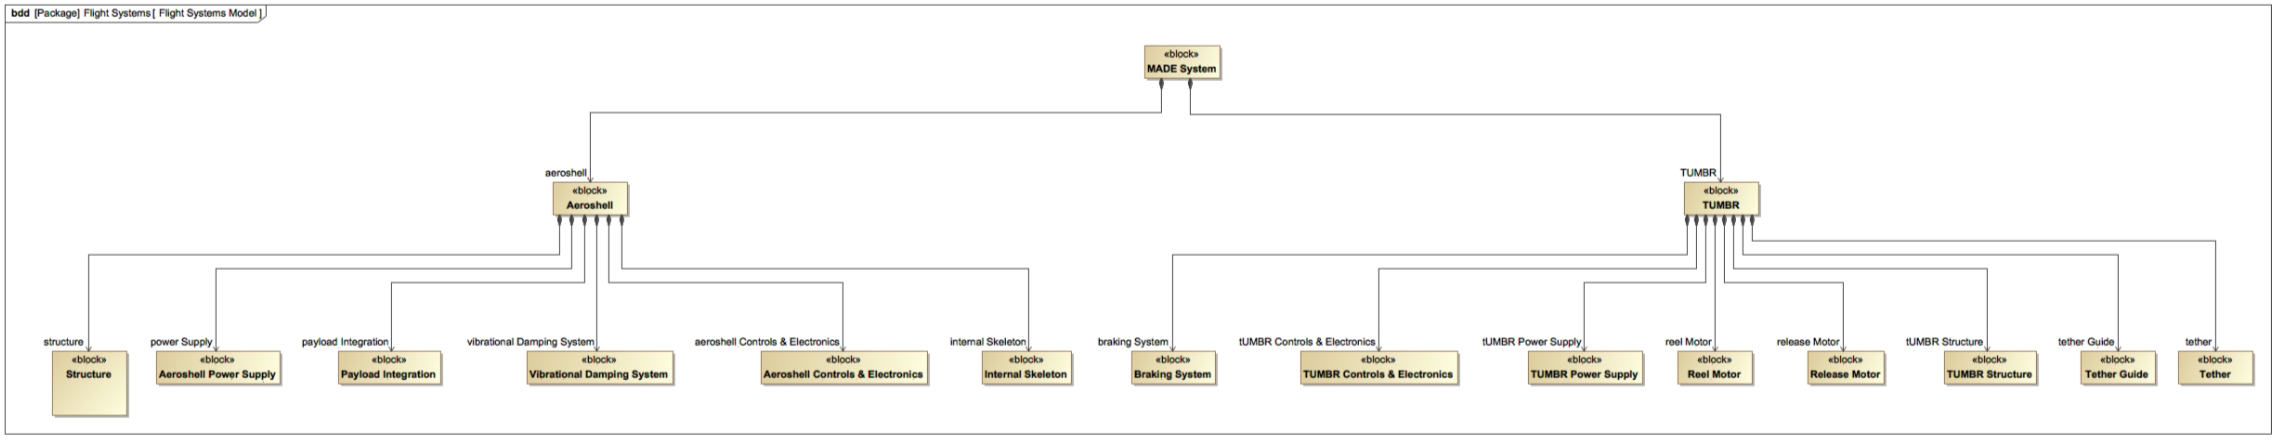
\includegraphics[width=.8\textwidth]{Figures/Stupid.png}
  \caption{\label{fig:CAMEO}CAMEO System Modeler of the ZAP-2 System}
\end{figure}

\subsection{Flight Procedure}

\indent\indent The missions begins when all systems are fully integrated and transported to the launch site, which at this point is TBD. Prior to launch, all systems are powered on and a communications check ensues to confirm that all systems are working and properly communicating to one another and with the ground station. The ZAP-2 system will then be mounted for launch. The tether will be completely reeled in with the brakes firmly compressing the rotor to make sure the tether and therefore aeroshell are held safely in place. With all status checks coming back nominal the ZAP-2 system will then be launched aboard World View's stratospheric balloon, the Stratollite. During the journey to the desired altitude of 30 kilometers, sensors onboard the aeroshell and TUMBR will track and record the temperature, pressure, humidity, and other key parameters. Climate control features such as heating pads will engage if necessary to keep all components within safe operating temperatures. Once at altitude the ZAP-2 will go through a pre-drop status check to ensure that all systems are still communicating, data is being logged, and the system is properly configured. At this point the ZAP-2 will commence its' first drop. 

To achieve this, the brakes which were engaged to hold the reel firmly in place will release the rotor allowing the entire reel to rotate. The release motor will engage just a fraction of a second later to being pulling the tether off of the reel. RPM sensors monitoring the angular velocity of the release motor and release disk will be recorded and sent to the Raspberry Pi units, which are controlling all motors and brakes. This sensory data will be used to create a closed-loop feedback system to precisely control the angular velocity of the release motor, ensuring that the tether will be ejected at the precise rate needed to prevent any tension from being present in the tether. 

During free fall and without any tension in the tether the aeroshell and its' payload will experience quality microgravity. Accelerometers and other sensors will record the forces experienced by the aeroshell and other parameters of the drop including time in free fall, temperature, pressure, and acceleration. Once the desired duration drop time has passed the braking system will engage and the aeroshell will gradually come to a full and complete stop. A status check will ensue to confirm that aeroshell is has come to a complete stop and that the reel is experience zero angular velocity. 

With confirmation that the system has fully stopped, the brakes will disengage, while in the same instant the reel motor will engage. The reel motor will rotate the reel causing the tether to reel in the aeroshell to begin its' ascent back to the TUMBR. Rotary sensors on the spool will monitor the progress while tether displacement sensors will monitor the length of tether that was not only release but is being reeled back in. A tether guide mounted to the TUMBR will ensure that the tether will be cleanly wrapped around the spool to prevent knotting and oversized coils. 

Once the control system senses that the appropriate amount of length of tether has been reeled back in, the motor will disengage while the brakes simultaneously engage to hold the reel, tether, and aeroshell in place. Another status check will take place to make sure the system is healthy and is ready for the next drop. Battery health will also be monitored to guarantee adequate power remains for subsequent drops. This information will all be then communicated back to the ground station where data will be reviewed and further commands to either continue or abort the mission will be sent back. Ideally, this process will take place at least six times to demonstrate the cost effective nature of this concept. After the multiple drops have taken place, the system will return back to the ground station where the payload will be retrieved and data recorded on the Raspberry Pi's will be retrieved and downloaded for posterity.

\subsection{Aeroshell}

\subsubsection{Aeroshell}

\indent\indent To determine which airfoils should be made into 3D CAD models, a 2D analysis in XFoil was done with 20+ different airfoils ranging in max thickness and the location of the max thickness along the chord length. This was done to save time instead of creating a CAD model for each airfoil to test within ANSYS. Each airfoil was scaled up to fit a middeck locker vertically within the aeroshell. The middeck locker was decided to be placed vertically due to the length of the aeroshell being substantially bigger if the middeck locker was placed horizontally. The Reynold's number and Mach number were calculated using the overall chord length as a reference length and the angle of attack was set to zero to determine the drag coefficient. This initial 2D analysis was compared to the previous iteration's airfoil and were tested at conditions of 30 Km with a speed of 247 m/s based on the previous iteration's calculations. Three airfoils were initially selected to create CAD models [Table~\ref{tab:xfoilanalysis}]. The code used to compute these values can be found in the Milestone III report in the Appendix section. Other key characteristics that were analyzed in XFoil were the pressure distribution curves and flow separation, transition, and reattachment to the airfoil. The flow separation can be seen on the $C_p$ distribution graph between the middle and trailing edge of the airfoil [Fig.~\ref{fig:flowseparation}]. The closer the flow separation difference means more skin friction drag, which would increase the drag.

\begin{figure}[ht]
  \centering
  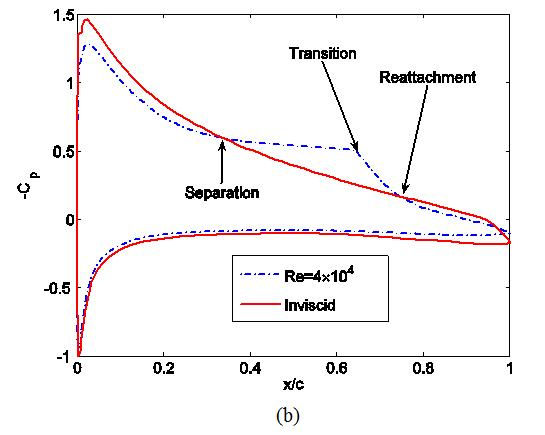
\includegraphics[width=.5\textwidth]{Aeroshell/flowseparation.png}
  \caption{\label{fig:flowseparation}Flow separation on $C_p$ distribution graph.}
\end{figure}

\begin{table}[H]
\caption{\label{tab:xfoilanalysis}XFoil 2D analysis.}
\centering
\resizebox{\textwidth}{!}{%
\begin{tabular}{|P{4cm}|P{5cm}|P{5cm}|P{4cm}|} 
\hline
Airfoil & Max thickness at Chord  & Est.Total Length & Drag Coefficient \\\hline

Green Team & 8.3\% at 20.2\% & 3.35 m or 11 ft. &0.03770 \\ \hline
ULTIMATE & 12.8\% at 34.2\% & 5.04 m or 16.5 ft. & 0.02925  \\ \hline
RAF 30  & 12.6\% at 30\% & 5.11 m or 16.8 ft. & 0.02954 \\ \hline
S8035 Aerobatic  & 14\% at 29.1\% & 4.46 m or 14.6 ft. & 0.02966  \\ \hline

\end{tabular}}
\end{table}

Optimization of the three airfoils was the next step to further decrease the drag and produce an efficient airfoil. The optimization code loads the desired airfoil within XFoil and calls XFoil into the Matlab code and starts "mutating" the airfoil until the optimizer has converged. This process took over 4,500 iterations to complete for these airfoils.  The optimized airfoil produced lead to the choosing of the Eppler E838 Hydrofoil. This airfoil had very similar characteristics to the optimized airfoil, but was slightly better in the key features of length, drag coefficient, pressure distribution and mass.

After choosing the airfoil that will be made into a CAD model to further test in ANSYS, it was found that the previous iteration's airfoil dimensions would not allow a full-size middeck locker to fit vertically within the aeroshell. So to accurately compare the two airfoils, the previous iteration's airfoil was scaled up by 1.15 times the original dimensions to fit a middeck locker vertically. An XFoil comparison was then completed between the Eppler E838 Hydrofoil and previous iteration's airfoil. The initial pressure at the leading edge and drag coefficient of the E838 Hydrofoil was significantly less than the previous iteration. The comparison of the two $C_p$ distribution graphs as well as $C_p$ vector distribution can be seen in [Fig.~\ref{fig:cp}] and [Fig.~\ref{fig:cpv}]. The conditions tested were at 30 Km and at 243.13 m/s, which was the calculated drop speed with a 15 m/s cross wind that could occur within the stratosphere.

\begin{figure}[H]
\centering
\begin{subfigure}[b]{.5\textwidth}
  \centering
  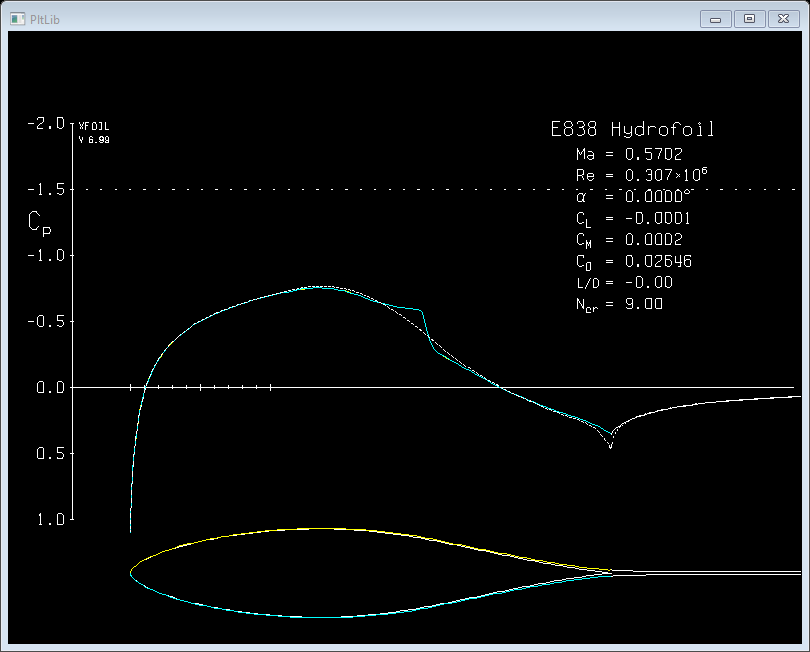
\includegraphics[width=0.9\linewidth]{Aeroshell/HydrofoilCp.png}
  \caption{\label{fig:hydrofoil_cp}E838 Hydrofoil $C_p$ distribution}
\end{subfigure}%
\begin{subfigure}[b]{.5\textwidth}
  \centering
  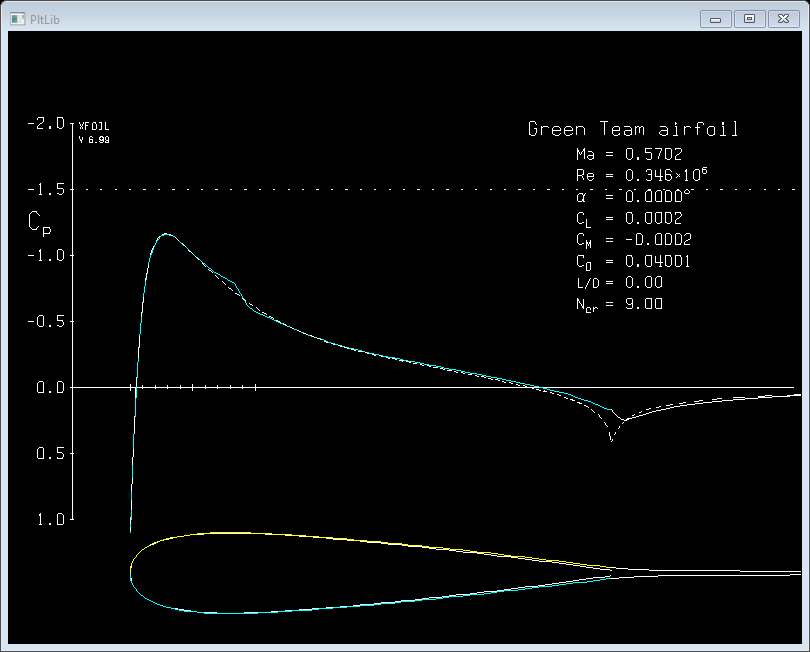
\includegraphics[width=0.9\linewidth]{Aeroshell/GreenTeamCp.png}
  \caption{\label{fig:greenteam_cp}Green Team airfoil $C_p$ distribution}
\end{subfigure}
\caption{\label{fig:cp}Airfoil $C_p$ distribution comparison.}
\end{figure}

\begin{figure}[H]
\centering
\begin{subfigure}[b]{.5\textwidth}
  \centering
  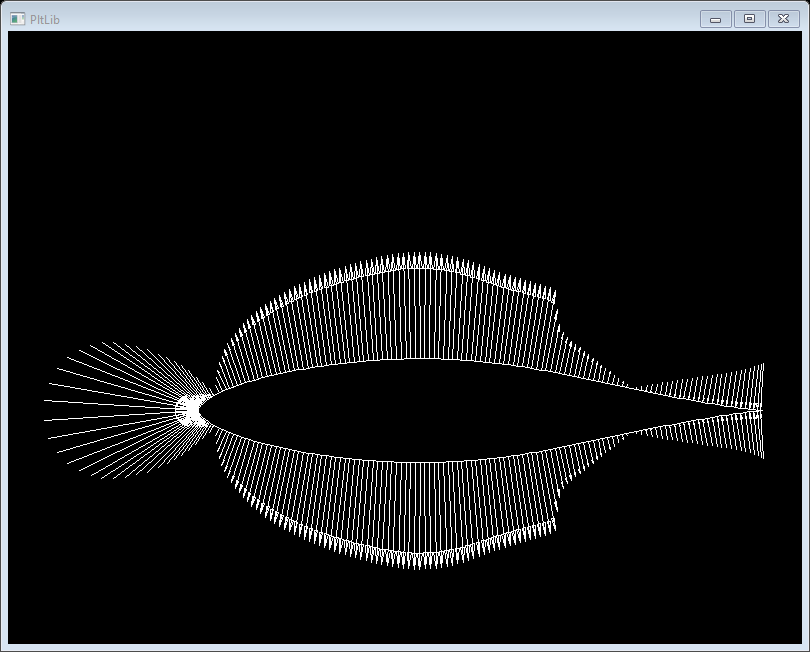
\includegraphics[width=0.9\linewidth]{Aeroshell/HydrofoilCpv.png}
  \caption{\label{fig:hydrofoil_cpv}E838 Hydrofoil $C_p$ vector distribution}
\end{subfigure}%
\begin{subfigure}[b]{.5\textwidth}
  \centering
  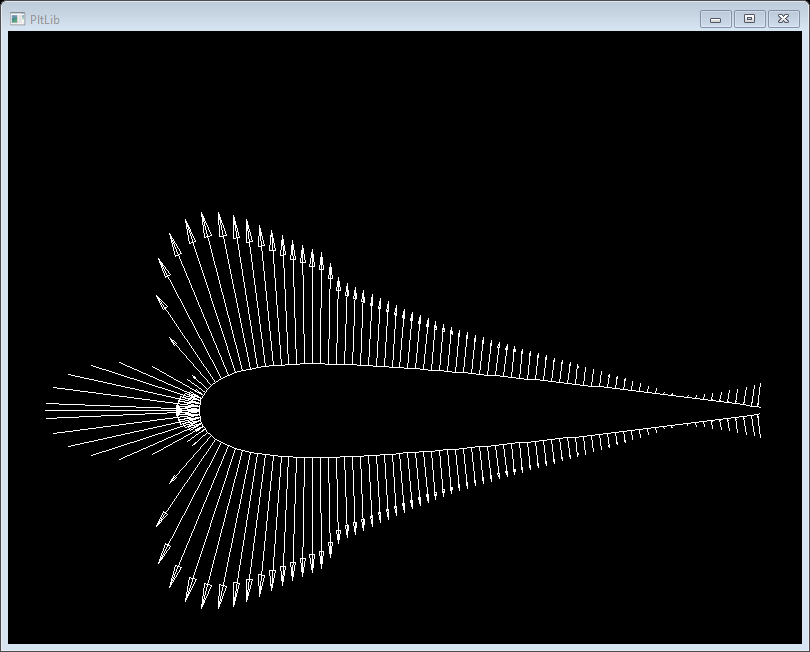
\includegraphics[width=0.9\linewidth]{Aeroshell/GreenTeamCpv.png}
  \caption{\label{fig:greenteam_cpv}Green Team airfoil $C_p$ vector distribution}
\end{subfigure}
\caption{\label{fig:cpv}Airfoil $C_p$ vector distribution comparison.}
\end{figure}

Based on the XFoil 2D analysis, the Eppler E838 Hydrofoil was chosen to be top priority for CFD testing. The other airfoils within the weighted ratings evaluation were also made into CAD models and the mass and length of these CAD models can be seen in [Table~\ref{tab:masslengthcompare}].

\begin{table}[H]
\caption{\label{tab:masslengthcompare}Airfoil mass and length comparison.}
\centering
\resizebox{\textwidth}{!}{%
\begin{tabular}{|P{4cm}|P{4cm}|P{6cm}|} 
\hline
Airfoil & Mass & Length   \\\hline

Green Team & 15.0 kg & 3.86 m or 12.7 ft. \\ \hline
Eppler E838 Hydrofoil & 12.74 kg &  3.42 m or 11.22 ft. \\ \hline
ULTIMATE & 24.0 kg & 4.86 m or 15.9 ft. \\ \hline
RAF 30  & 24.9 kg & 4.94 m or 16.2 ft. \\ \hline
S8035 Aerobatic & 21.5 kg & 4.39 m or 14.4 ft. \\ \hline

\end{tabular}}
\end{table}

\indent\indent To ensure the aeroshell can withstand the forces and enviornmental conditions it experiences, and to aid in the ease and repeatability of manufacturing the aeroshell, carbon fiber will be used as the main body material. Carbon fiber is a strong choice for this application because of the complicated geometry of the aeroshell. Where other materials would require expensive and complicated machining methods carbon fiber can be shaped as a fabric to a mold, then fixed into the desired shape with epoxy and hardener. Carbon fiber is also excellent in axial and sheer strain, which are the types of forces expected to appear near the internal structure hardpoints and the latch connection points on the aeroshell. Since the design has shifted away from the load of the payload acting through the carbon fiber as in the first iteration of this project and toward the load acting through the internal structure, the aeroshell must now only be strong enough to bear its own weight under rapid breaking. This allows the design to use fewer layers and reduce weight. Carbon fiber is also thermally stable, which will minimize complications due to a high altitude enviornment and high speed friction conditions.

The carbon fiber mold that will be used for this iteration of the project will be constructed from numerous 1/4 inch sheets of laser cut MDF board, forming a ribbed cast of the aeroshell. The gaps between the wood will be filled in with expanding foam and packing peanuts to ensure the fixture remains rigid. The main surface of the mold will be covered in Bondo and thoroughly sanded to form the intended shape. Once the correct shape is achieved, a finish will be applied to ensure the carbon fiber aeroshell has a smooth finish after debonding.

\subsubsection{Internal Structure}

\indent\indent The internal structure was not considered in the previous iterations design, so this system had to be designed from the ground up to fit within the aeroshell. With the goal of minimizing drag driving the external aeroshell design, the internal structure's primary constraints were the internal volume of the aeroshell and mass, to keep the total system under the 400 kg mass budget. To keep the aeroshell cross sectional area minimal, the internal structure was designed to use the volume between the rectangular middeck locker and circular aeroshell, such that the largest diameter fits the customers payload dimensions. The primary structure material was chosen to be extruded 8020 aluminum for weight, ease of assembly and manufacturing, with mounting plates made of CNC machined aluminum. The internal structure needs space to mount electronics for environmental sensors and communication with the platform, and also have room to potentially mount a propulsion system to counter drag force and attain microgravity in future iterations. The selection of 8020 as the main structure components allows for easy replacement of parts and also modularity for specific flight circumstances as needed, such as additional mounting points.

\begin{figure}[H]
\centering
\begin{subfigure}[b]{.3\textwidth}
  \centering
  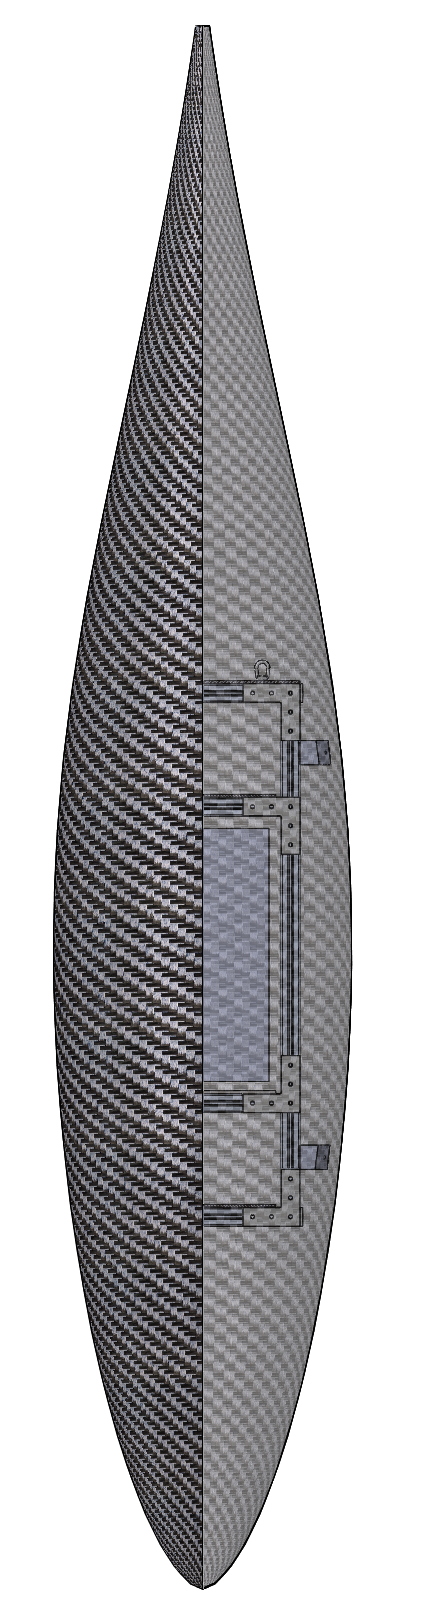
\includegraphics[width=0.5\linewidth]{Aeroshell/StructShell.png}
  \caption{\label{fig:structshell} Aeroshell}
\end{subfigure}%
\begin{subfigure}[b]{.3\textwidth}
  \centering
  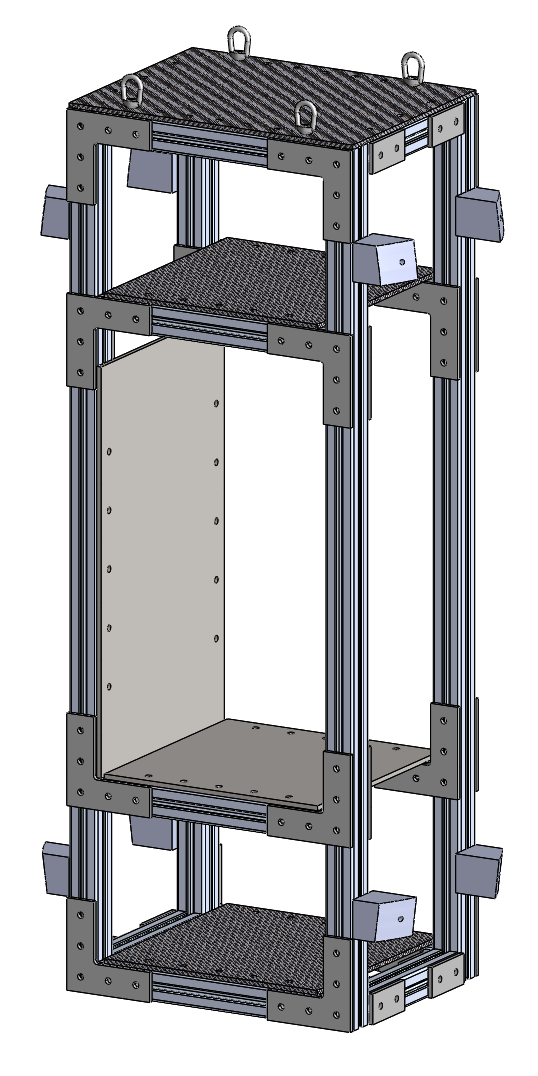
\includegraphics[width=0.8\linewidth]{Aeroshell/StructNoshell.png}
  \caption{\label{fig:structnoshell} Internal Structure}
\end{subfigure}
%\caption{\label{fig:internalstructure} Internal Structure}
\end{figure}

\indent\indent Two different tether attachment options were considered, a frustum shape component at the end of the aeroshell, and a means of attaching the tether directly to the internal structure. Initial design looked at the frustum design option. With this option, the aeroshell would bolt onto this conically shaped component and the tether would attach to the top via a significantly large bolt to hold the load. However this component would be heavy, complex, and expensive to manufacture and implement, as well as causing all load transfer to pass through a single point as well as the carbon fiber aeroshell itself which would complicate analysis and design, requiring significant reinforcement to guarantee low chance of failure under loads experienced during braking.

The second option, and the one chosen, was to attach the tether to the internal structure instead of the aeroshell. The structure, being made of aluminum, has isotropic properties so it is able to be more easily analyzed, requires less additional components to implement which saves mass, and eliminates a possible single point of failure by spreading the connection to 4 individual points. This tether attachment method was composed of 4 eye nuts connected to the top of the internal structure with 5/16" bolts passing through two parallel 8020 beams. This disperses the load across 4 different points, reducing the strength needed by each point. This method adds minimal additional weight for the hardware needed over a design that attaches to the aeroshell first. This connection will need heavy lifting hooks, capable of locking to prevent accidental disconnection and also swiveling to prevent twisting the tether during drops.

With the tether attaching internally, the aeroshell needs to mount to the internal structure. The structure will be the component experiencing the majority of the loads of braking, so the mounting points of the aeroshell will mostly experience forces due to the mass of the aeroshell. This reduces the strength required of the mounting points. Due to the irregular shape of the internal surface of the shell, any secure connection between the shell and structure will need to be custom mounting blocks machined to the shape of the desired contact point of the shell. These blocks bolt to the structure and the aeroshell will be placed against them in the appropriate position to be bolted to the structure. Current design has 8 mounting blocks total, with 8 external bolts on the outside of the shell which is significantly less than the previous iterations. This will help reduce anomalies with flow along the aeroshell.

\subsection{TUMBR}

\subsubsection{Tether}

\begin{table}[H]
\caption{\label{tab:tether_01}Tether materials and properties.}
\centering
% You need as many of these as you have columns i.e 3 columns ==> {l|c|c}
% To control width of a box you must be "hack-y" and treat the cell as containing a paragraph i.e use P{width}
\resizebox{\textwidth}{!}{%
% \rowcolors{2}{gray!25}{white} 	% This line adds alternating row colors, I'll leave it up to you to figure out the parameters to it
\begin{tabular}{|P{6cm}|P{6cm}|P{6cm}|} 
\hline\hline
Material & Tensile Strength (MPa) & Density (Kg/m3) \\\hline

Kevlar 29 & 2,920 & 1,440 \\ \hline
Kevlar 49 & 3,000 & 1,440  \\ \hline
Kevlar AP  & 2809 & 1,440 \\ \hline
Spectra-1000 (75)  & 3,680 & 970  \\ \hline
Spectra-1000 (180)& 3,250 & 970 \\ \hline
Spectra-1000 (375-189) & 3,000 & 970  \\ \hline


\end{tabular}}
\end{table}

The previous team decided Spectra by Honeywell would be the most suitable option for the tether material. Our team is continuing with this choice for several reasons. Spectra is resistant to chemicals, water, and ultraviolet light. It is also capable of withstanding high-load strain-rate velocities. Spectra is also lighter than kevlar. This will lessen the load put on the reel motor as well as help stay within the mass budget.

\subsubsection{Tether Guide}

\indent\indent The implementation of a tether guide is important for the platform to perform multiple drops. If the tether is not evenly wound across the reel then knotting can occur and completely stop the aeroshell from dropping. The previous team came up with a design for a tether guide, but were unable to integrate it. It used a traverse roll and clutch mechanism to guide the tether as it was reeled up. This concept was compared to another option for a tether guide called a rolling ring drive. The rolling ring drive was already assembled and simple to implement. It accomplished the same task with less risk of failure. For this reason it was decided to use the rolling ring drive. A motor from the last iteration of the project will be reused with this design. A v-belt and pulley system will act as the transmission.

\subsubsection{Brakes}

\indent\indent The braking component of the prototype is a mission critical component which, if it were to fail, will render the mission useless. The first generation incorporated one type of braking system, a rotor and caliper friction setup, which is commonly found in automobiles. For the second generation of prototype (ZAP-2), two different types of braking will be combined and incorporated into the whole system to ensure a repeatable and reliable deceleration experience. The two types of brakes which will be incorporated are an electromagnetic system and a frictional system. These two types of braking will work in tandem as each type has its strengths and weaknesses. In short, the electromagnetic braking will occur for the initial deceleration of the aeroshell since the braking force is proportional to the velocity of the aeroshell. Once the aeroshell is slowed to a reasonable speed, the friction braking system will then be used to slow the aeroshell to a halt.

\begin{figure}[!ht]
\centering
\begin{minipage}{.5\textwidth}
  \centering
  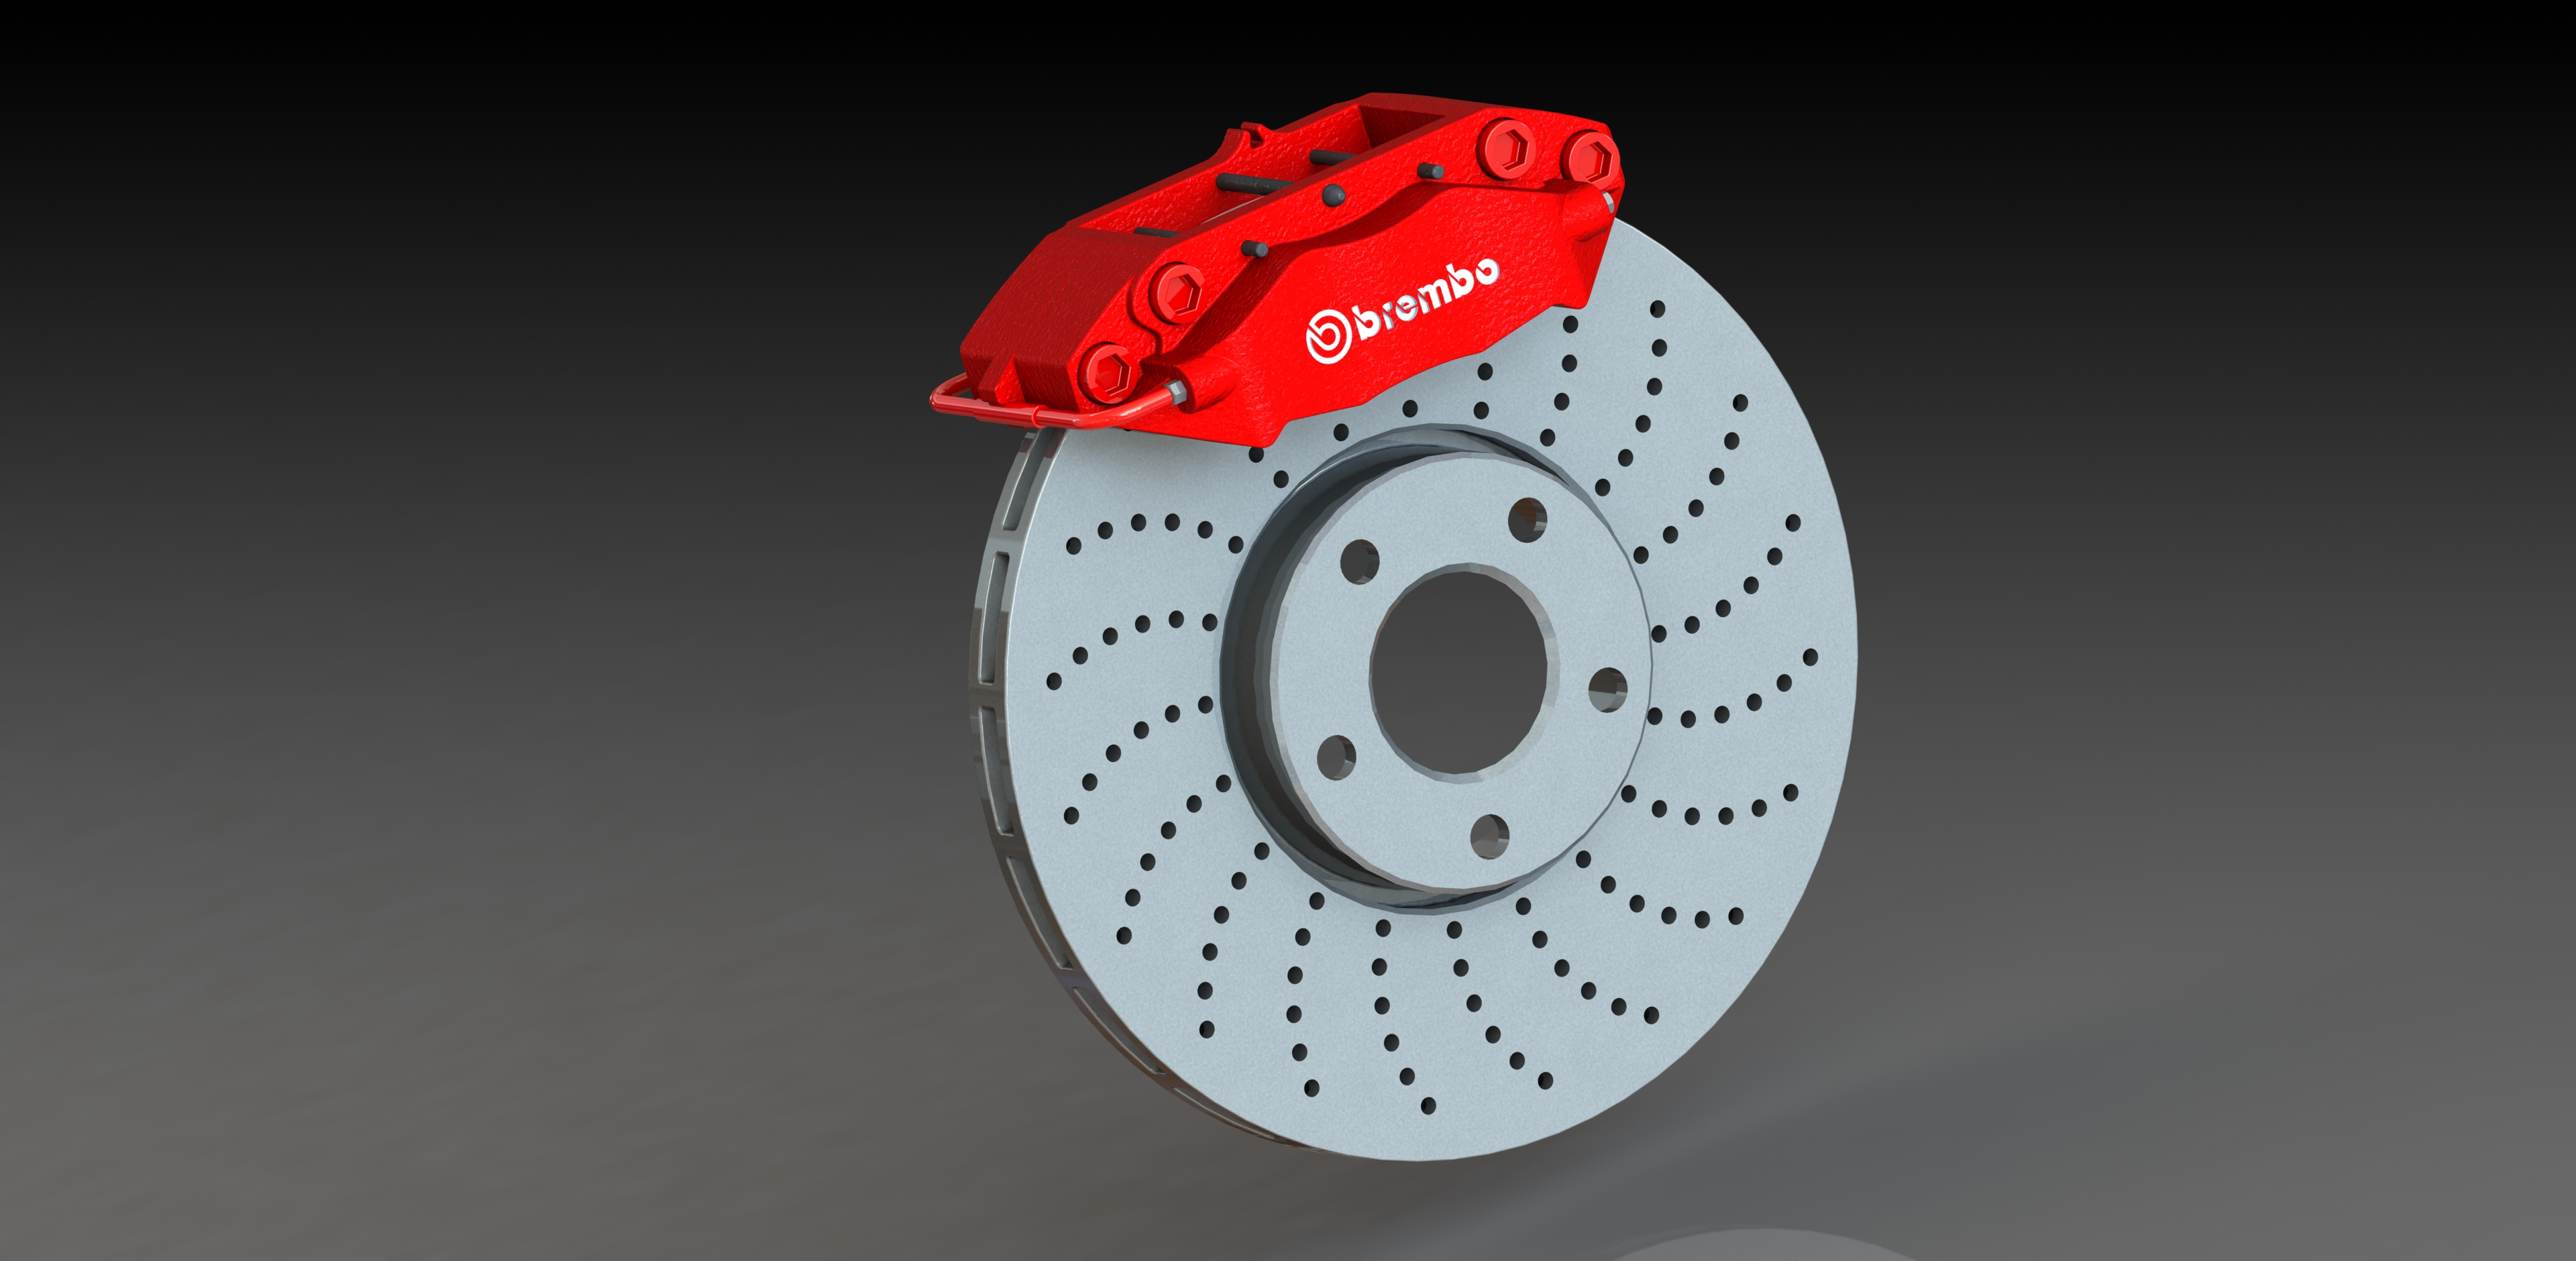
\includegraphics[width=0.9\linewidth]{TUMBR/CaliperRotor.png}
  \caption{\label{fig:DiscBrake}Rotor and caliper}
\end{minipage}%
\begin{minipage}{.5\textwidth}
  \centering
  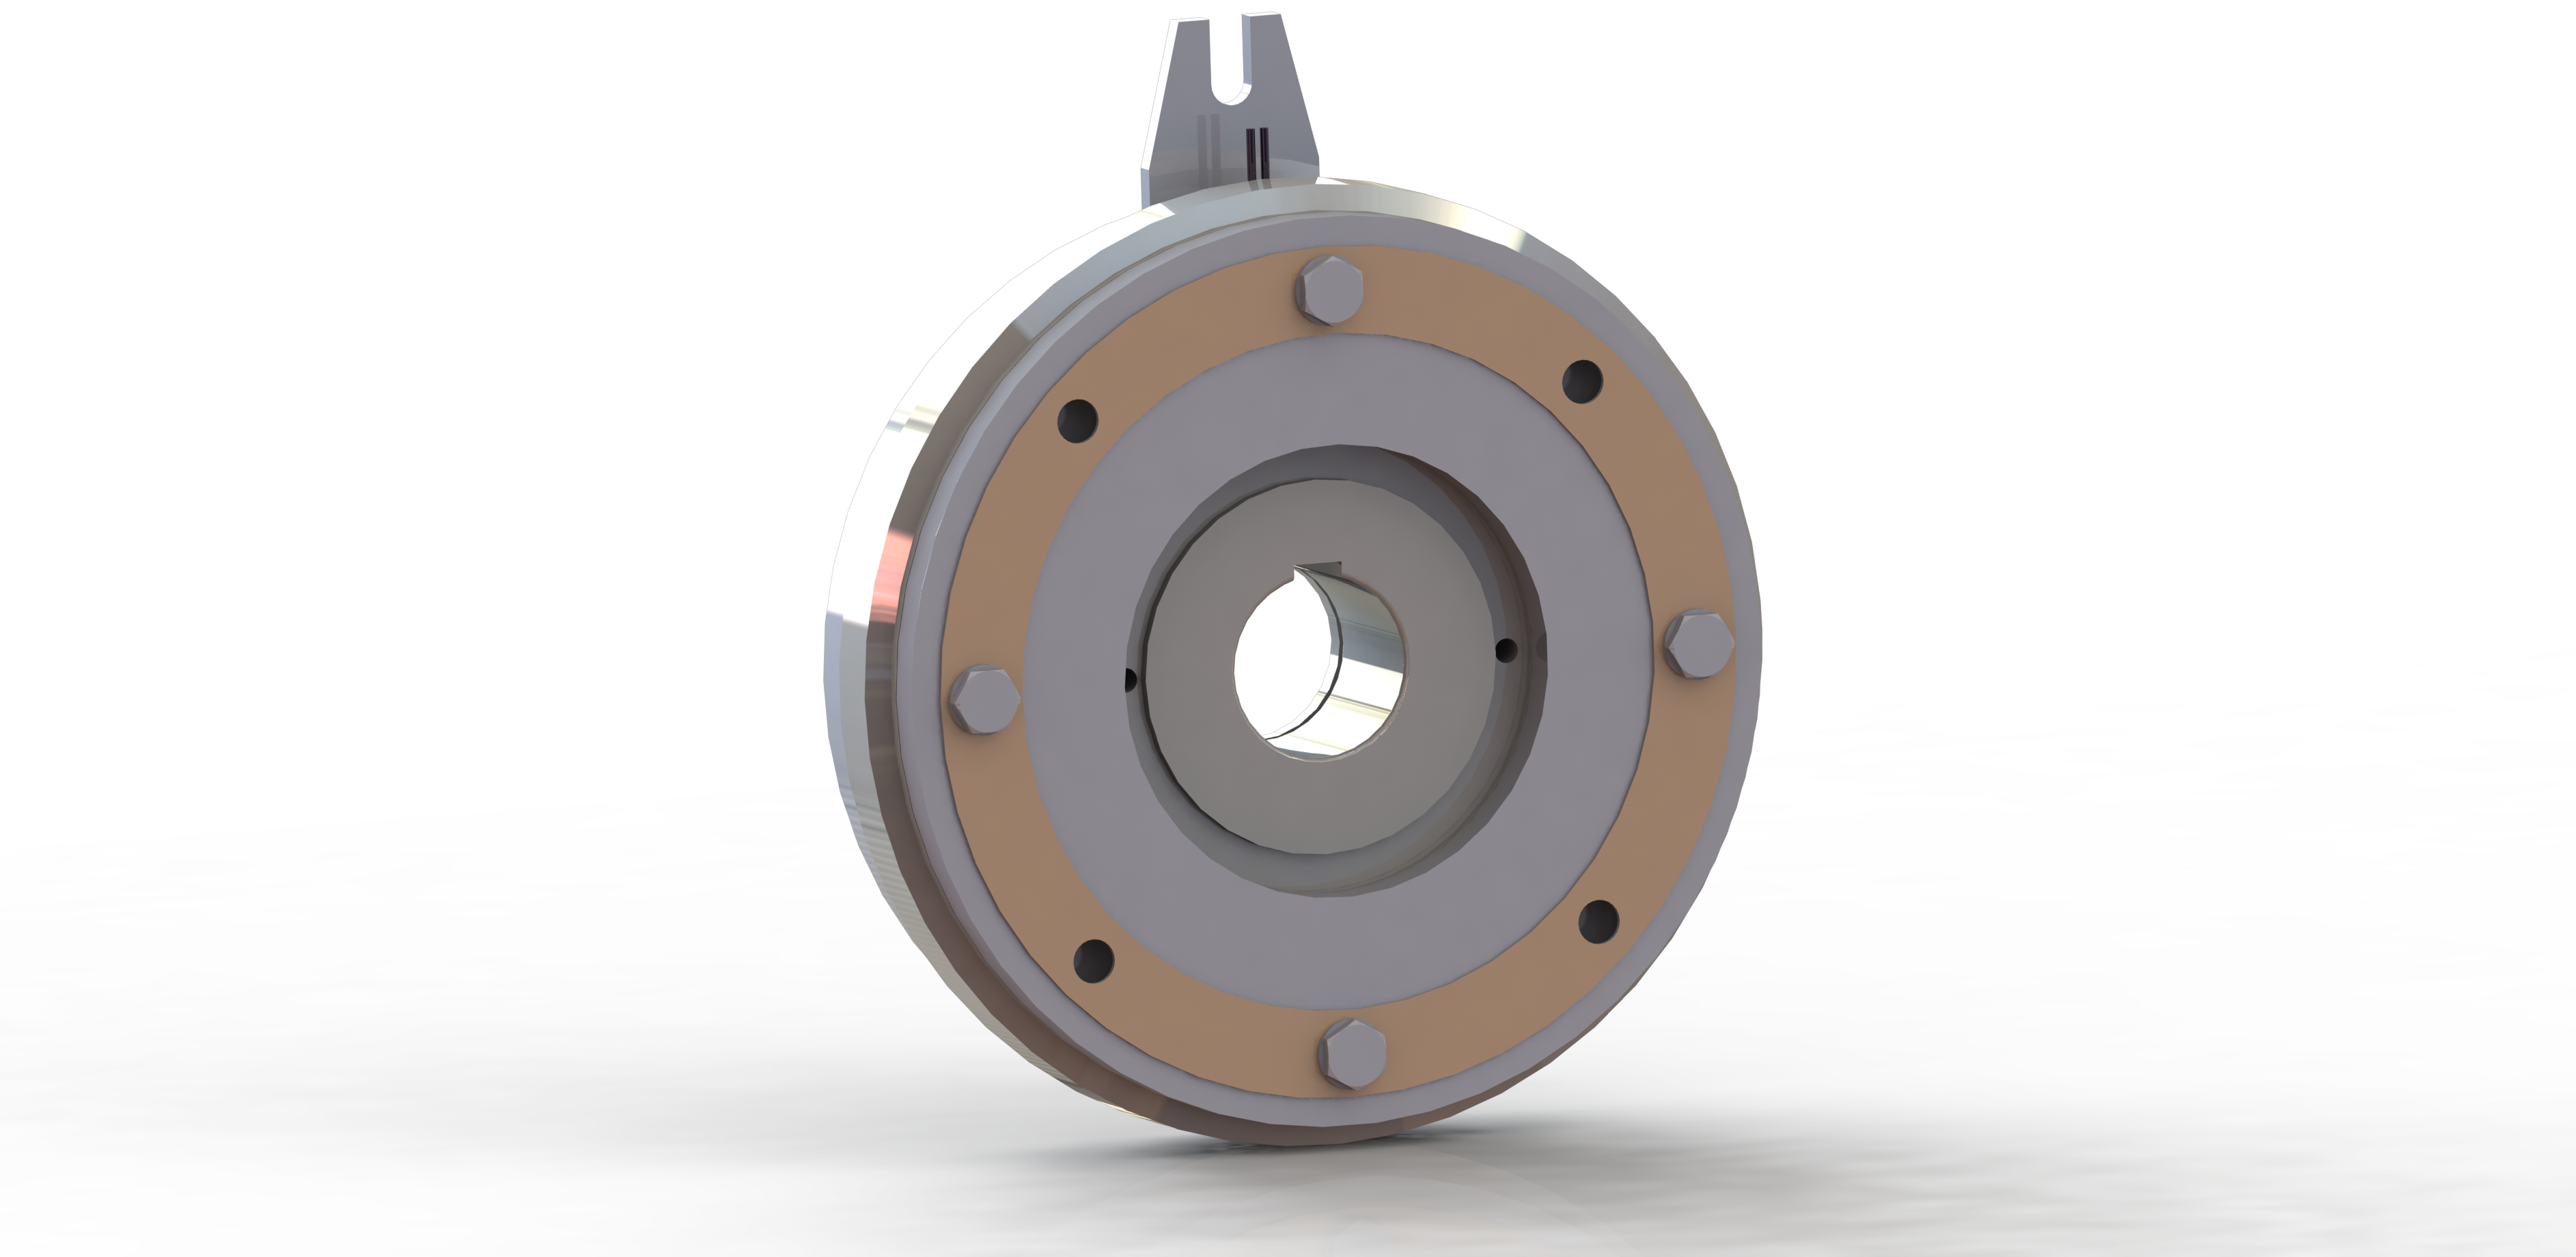
\includegraphics[width=0.9\linewidth]{TUMBR/EM.png}
  \caption{\label{fig:Electro}Electromagnetic}
\end{minipage}
\end{figure}

\indent\indent To assist the frictional system in braking an electromagnetic system will be used in tandem to lower the risk of failure when decelerating. Electromagnetic braking was chosen because the force generated is proportional to the angular velocity of the rotor with a higher upper limit of maximum RPM able to withstand. The system will be used for the beginning portion of the deceleration where the RPM is very high, and then be handed off to the frictional braking when the RPM reaches an optimal speed. While it sounds like the electromagnetic braking can perform all the same functions of the frictional braking without the problems associated, this can be a misleading assumption.  The reason for the need of frictional assistance is as stated above: the force applied for braking is proportional to the angular velocity of the shaft. This means that as the velocity of the shaft comes to zero, the force that the electromagnetic system can apply to the shaft is also zero. In short, the electromagnetic braking system can be very useful to slow down a system with high angular velocity, however when reaching a small to zero angular velocity the electromagnetic braking will not be able to bring the system to a halt. The proposed solution is to use both the electromagnetic braking (for high RPM) and frictional braking (for lower RPM) and bring the system to a halt.

\begin{figure}[H]
  \centering
  \includegraphics[width=.7\textwidth]{TUMBR/Brake_Setup2.JPG}
  \caption{\label{fig:com}Combined braking system.}
\end{figure}

\indent\indent The first design created [Fig. ~\ref{fig:single}]is using a single rotor and caliper attached to the shaft. This design is very similar, if not the same, to the design of the previous team's braking system. The simplicity of the design will ensure an easy integration into any system with minimal weight needed. Problems which can arise from this design include: an increased brake time due to the lack of maximum output force of one caliper and increased wear on the brake pad which can lead to possible failures in the later drops of the flight.

\begin{figure}[!ht]
  \centering
  \includegraphics[width=.7\textwidth]{TUMBR/SinglerotorSingleacaliper.png}
  \caption{\label{fig:single}Single rotor and caliper setup}
\end{figure}

\indent\indent The second design created [Fig. ~\ref{fig:Dualcaliper}] is using a single rotor and dual caliper attached to the shaft. this design is to maximize the stopping power available in a small, simple, light weight package. With four brake pads in contact with the rotor the stopping distance, brake pad wear, and time to reach zero velocity will be minimized. A problem which can arise in this system is a large increase in thermal energy in both the rotor and brake pads due to increased stopping power which can cause brake fade and/or rotor warpage.

\begin{figure}[H]
  \centering
  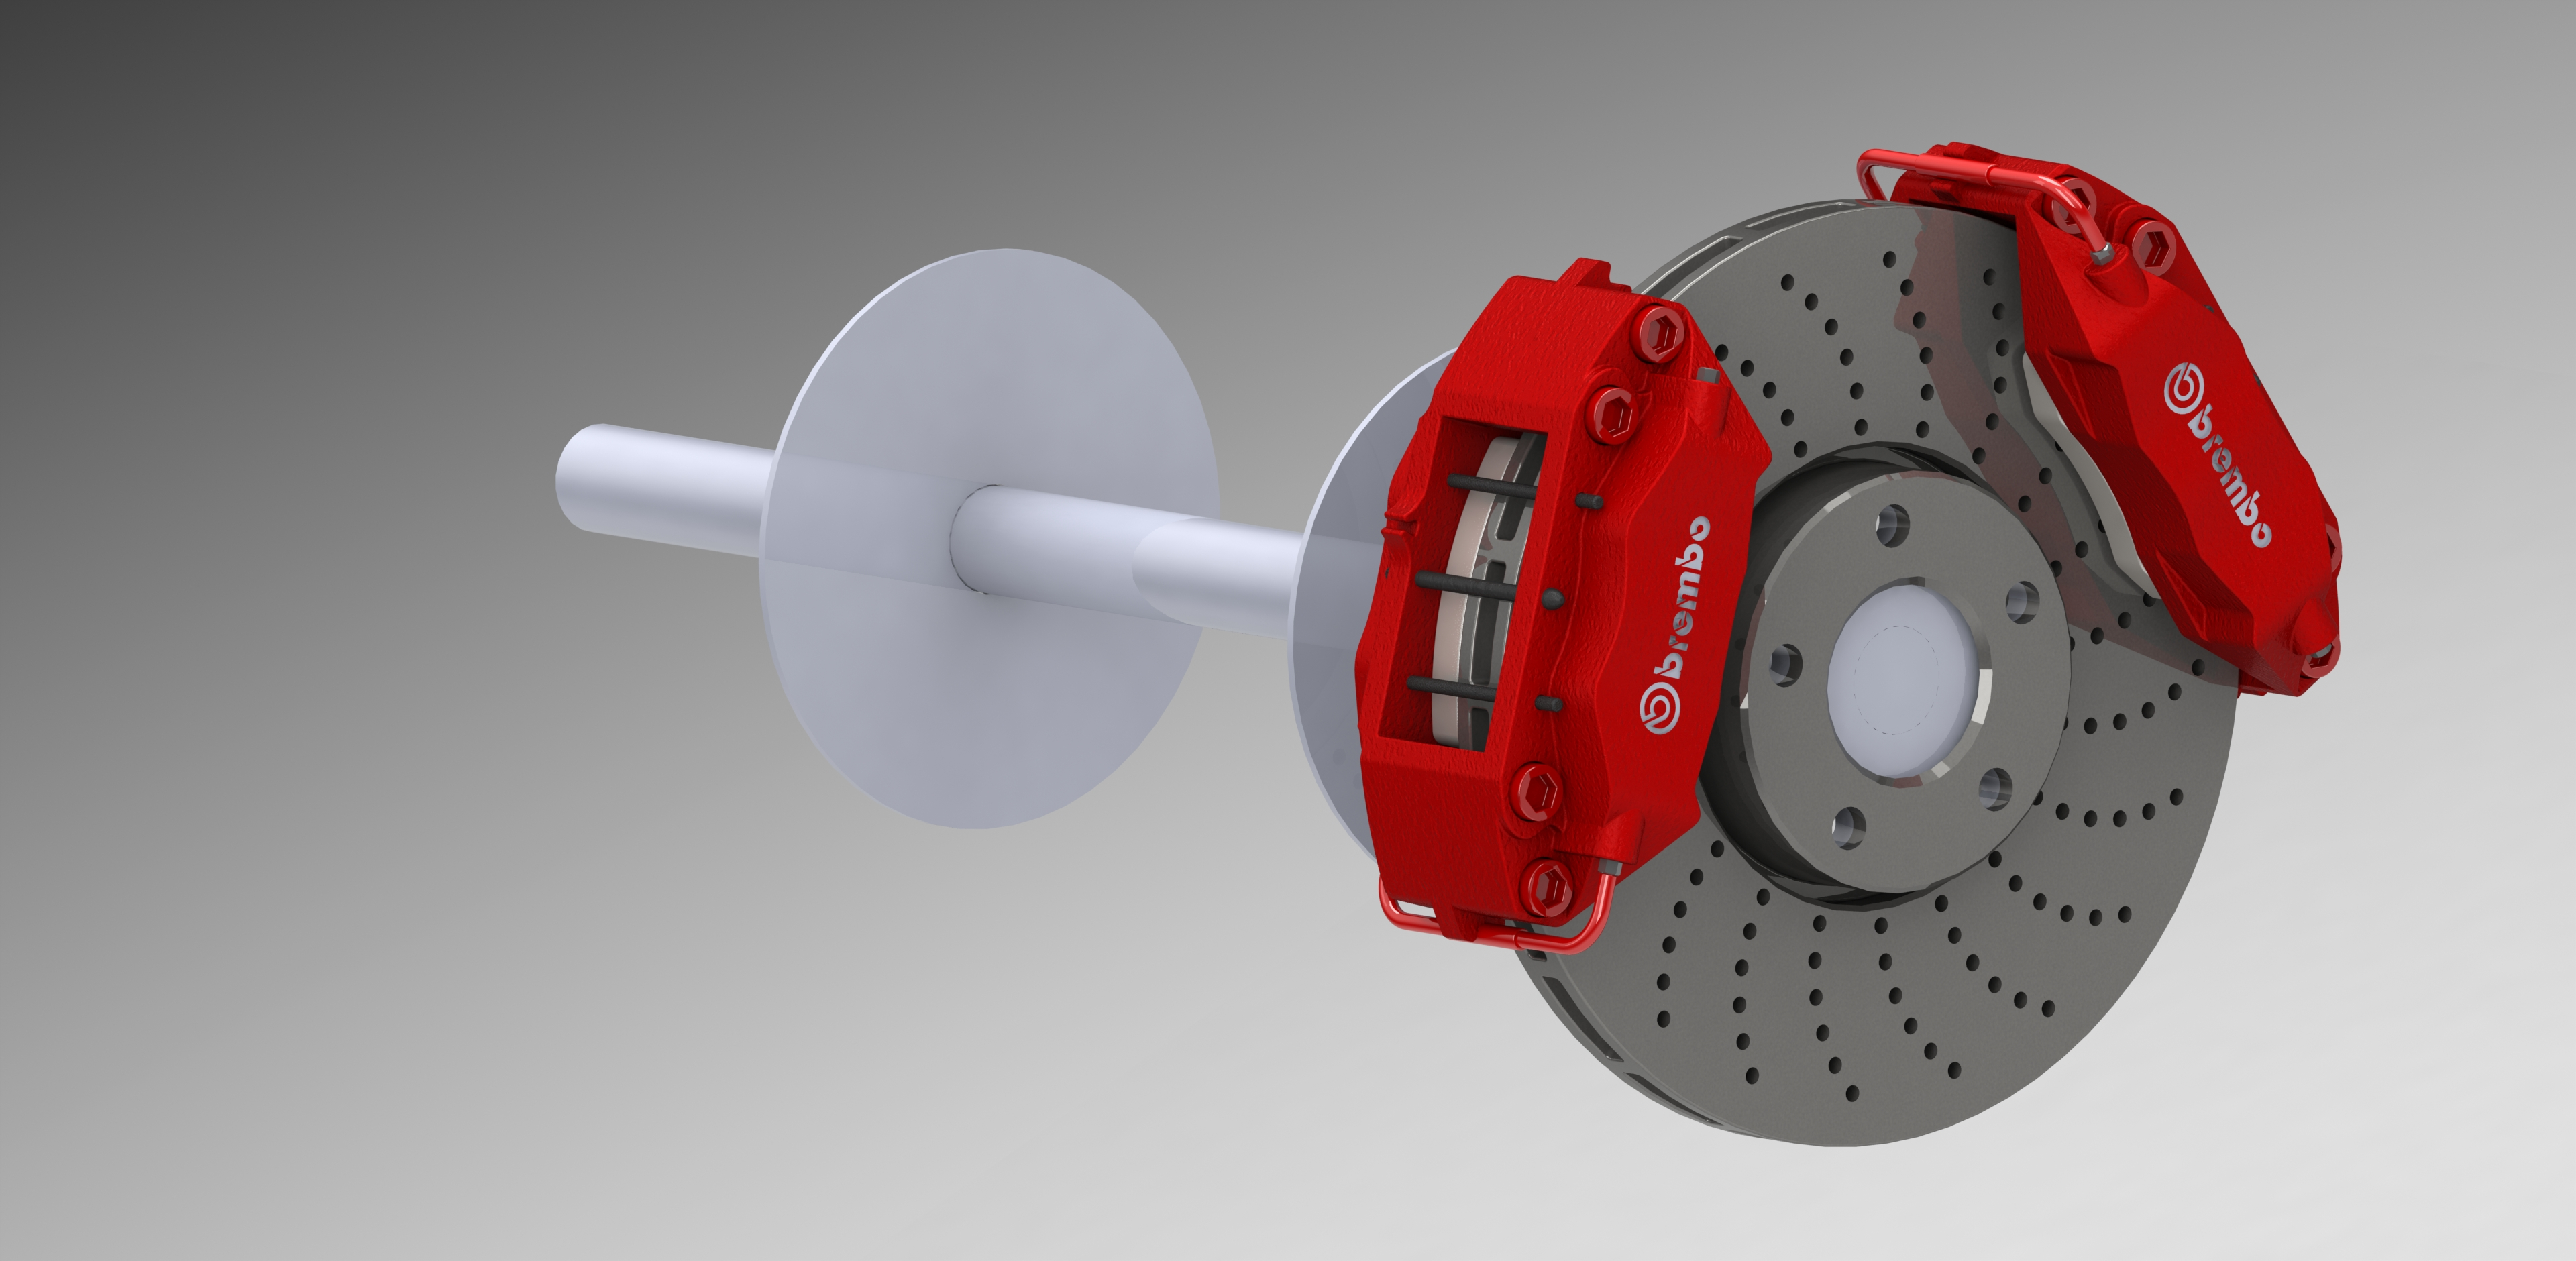
\includegraphics[width=.7\textwidth]{TUMBR/DualCaliper.png}
  \caption{\label{fig:Dualcaliper}Dual caliper on a single rotor}
\end{figure}

\indent\indent The last brake configuration [Fig. ~\ref{fig:dualrotor}] has in total two rotors and calipers. This configuration is much like the that of the single rotor, however with thermal energy and load distributed between two rotors. The downside of this configuration is the weight aspect. However, if using modern materials such as carbon-ceramic or carbon-carbon the total weight of both rotors and calipers can be lower than a single iron rotor without the caliper. This system ensures that the amount of force needed to brake will be available and the thermal energy will be distributed between two rotors which will minimize the probability of brake fade and thermal warpage. This setup is ideal for the prototype and would be preferred over the other two due to its ability to split the load and thermal energy between two points. 

\begin{figure}[H]
  \centering
  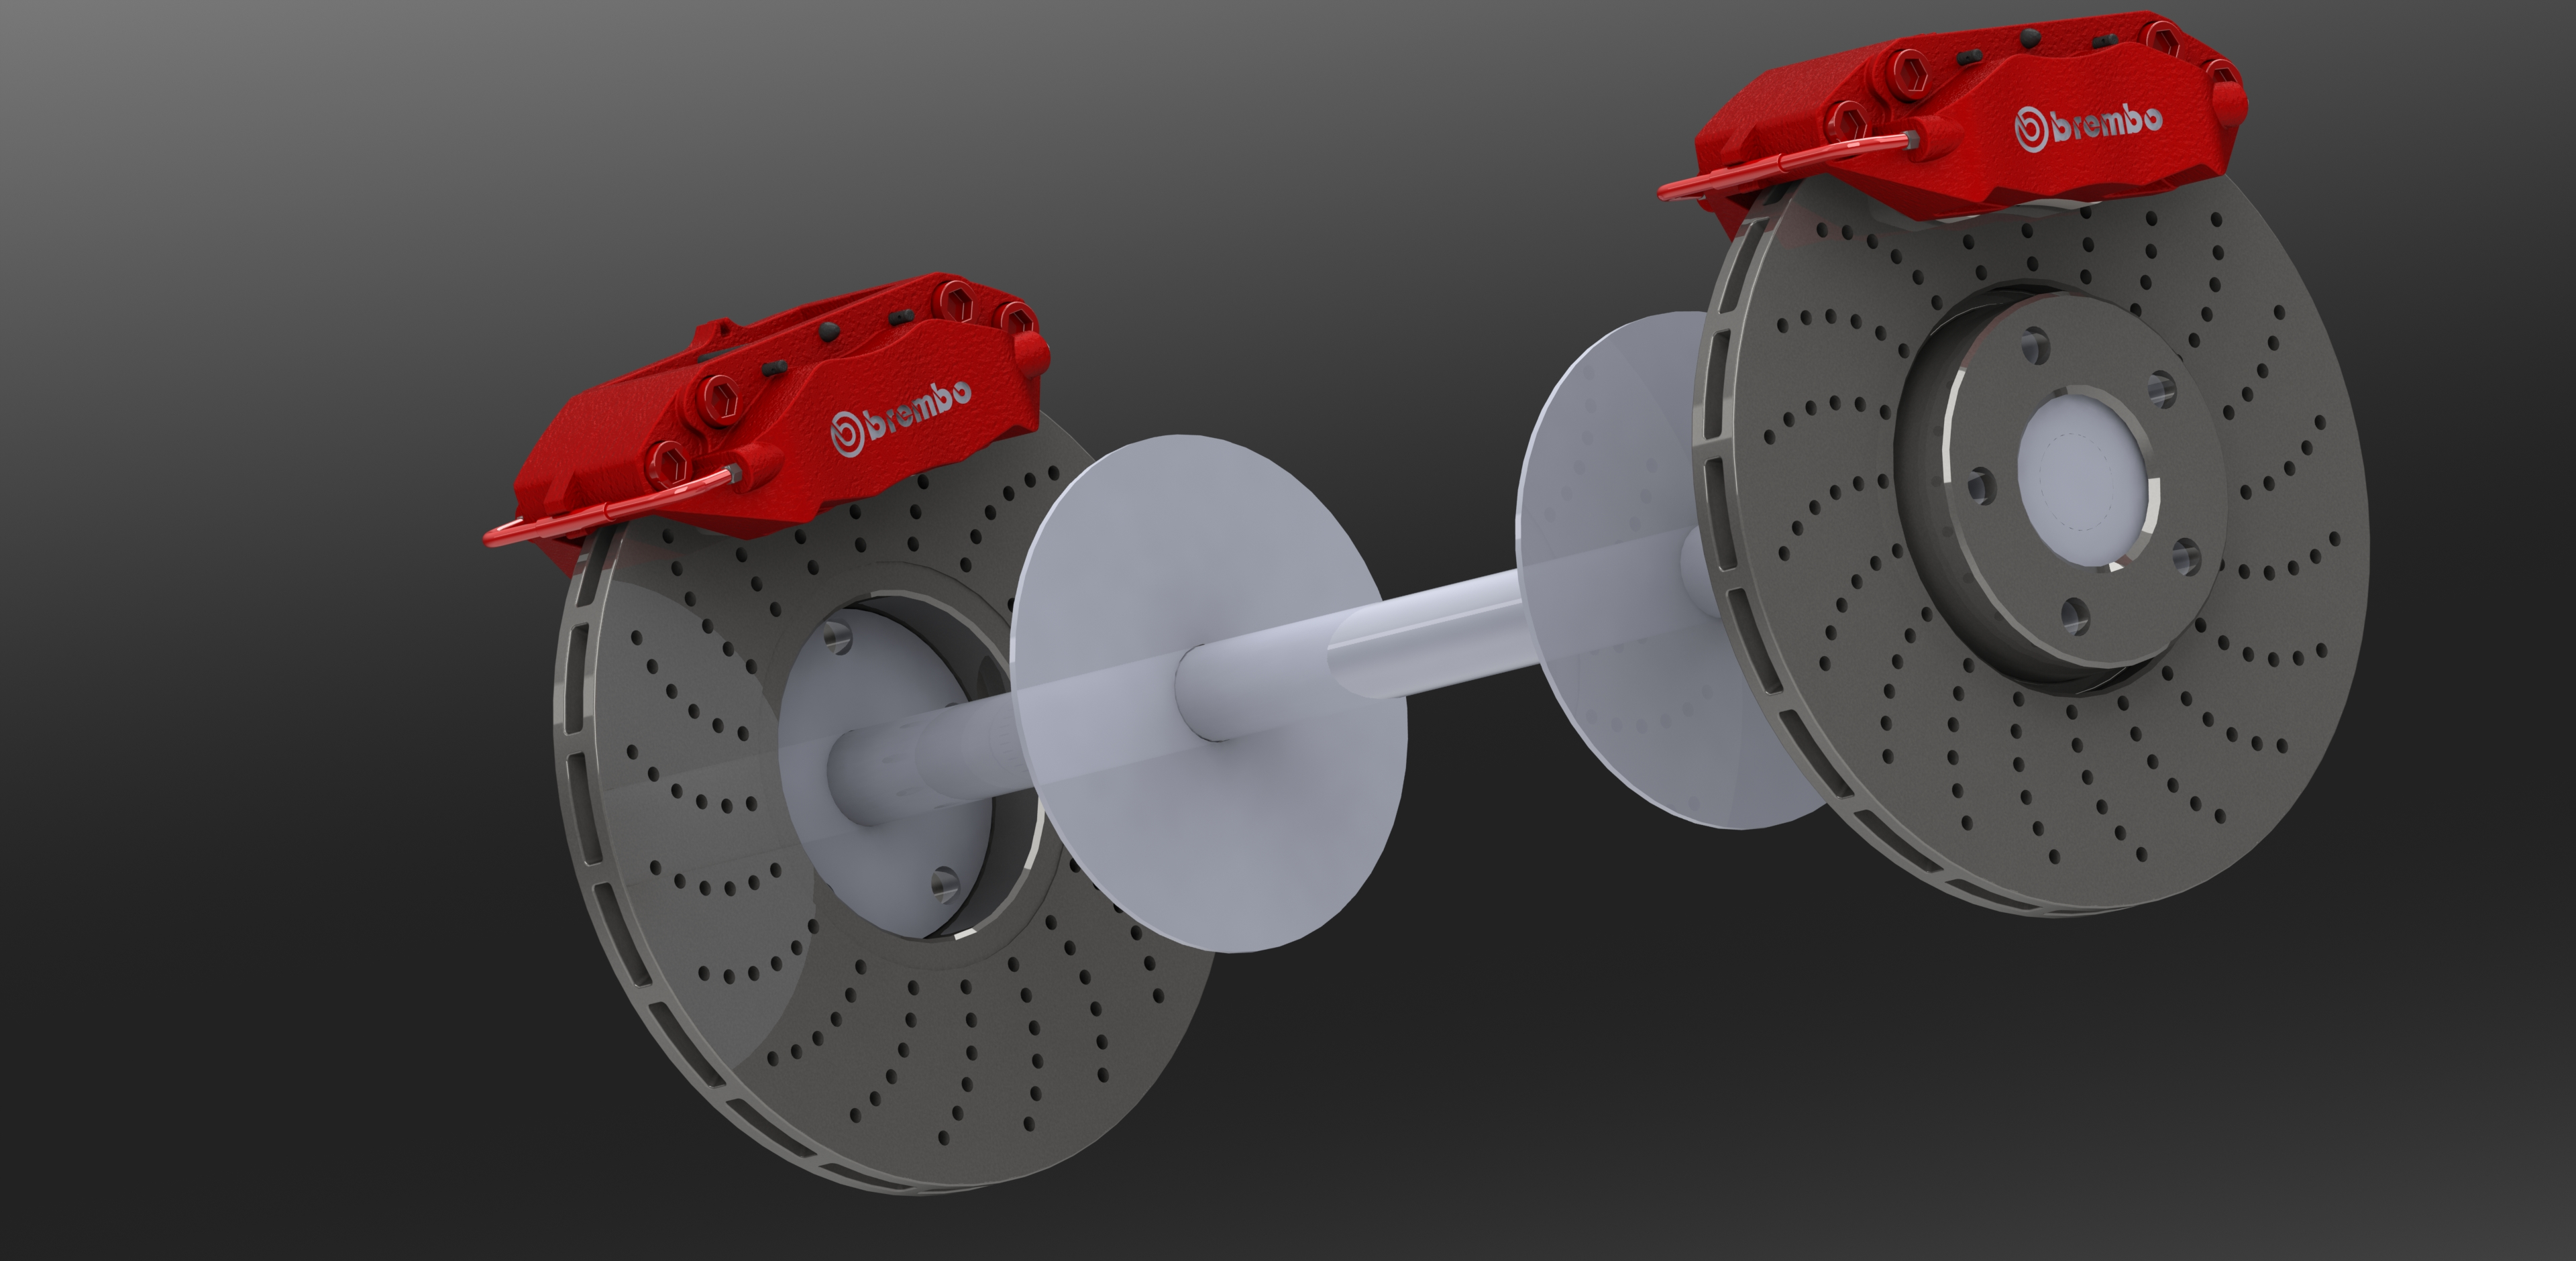
\includegraphics[width=.7\textwidth]{TUMBR/DualRotorRender.png}
  \caption{\label{fig:dualrotor}Dual rotor and caliper setup}
\end{figure}

\subsubsection{Frictional Braking}

\indent\indent Frictional braking has large limitations with respect to material strength, temperature and lifespan. The frictional material has a certain shear stress it can undertake before failure; the shear stress is caused from the angular velocity of the rotor and the force which is applied to the material when both are in contact. The maximum revolutions per meter (RPM) calculated from the top speed of a F1 is 1,450 RPM, while the rotor on the unit will be experiencing  approximately 5,500 RPM (at 9 seconds of drop time). The RPM experienced by the braking system will be an five times larger than that of the F1 car. This vast difference in RPM causes is very high probability that the brake pads will encounter too much shear stress and will seemingly disintegrate when a force is applied. The next problem encountered is the amount of thermal energy generated from the braking process itself. With large temperatures the coefficient of friction felt between the pad and the rotor diminishes causing a significant decrease in braking force. Since the most common type of rotor used is usually cast iron or an iron alloy, when a large temperature is applied the iron is prone to deformation. This deformation can completely lock the system in place and render all functions of moving the aeroshell to and from the unit as useless. When under heavy load and high temperatures, both the rotor and the pads experience immense wear and exponentially decreases the lifespan of the two objects. This can be an issue since the braking needs to perform reliably and accurately for a total of eight drops during a single flight. These three main issues prompt the consideration of an additional system of deceleration to assist the frictional braking in order to prevent these common failure points.

\indent\indent There are many different types of braking techniques that use friction in order to bring the subject of matter to a velocity of zero. These types of braking include drum brakes, band brakes, disc brakes, rotor and caliper brakes, and shoe brakes. The second generation prototype will use a refined and redesigned rotor and caliper brake setup that was incorporated in the first generation prototype. These brakes are very common and often used in automobiles in order to bring them to a halt. Rotor and caliper brakes are very reliable, easily sourced, modifiable, easily maintenanced and have a long life span. Drum brakes were previously very common in cars until replaced by the rotor and caliper setup. The drum brake system enclosed inside a metal shell which houses all the components and because of this enclosure, it can be difficult and time consuming to preform frequent maintenance on the system. Band brakes are typically made from a flexible material (normally a type of rubber) which in semi-warm climate will preform well. However, when in -46 \degree Celsius climate the flexible material will no longer be flexible. Almost all types of rubber, with the exception of a select few, will become hard and brittle in this temperature and will not preform the braking required.

\indent\indent Within the rotor and caliper setup, there are many different materials and geometries that can be used for the rotor and brake pads (which lay inside the caliper). The combination of these materials and geometries is very important based on the type of application necessary. For the standard car, an iron rotor is used for its high thermal conductivity, low manufacturing cost, large lifespan, and great reliability. Most of these iron rotors don’t undergo a very stressful environment which pushes the material to its limits. When iron rotors are subjected to a stressful environment common failures include a deformation of the rotor and the lowering of the coefficient of friction between the rotor and the brake pad (brake fade). For this reason, high performance cars use a composite material of silicon carbide ceramic which offer much better performance under a stressful environment. Ceramic rotors are very common in high performance cars for the large heat capacity ability property of the material. These rotors can undergo temperatures of around 1,350 \degree C before deforming or failing and are a much lighter alternative to cast iron. The final type of rotor are Carbon carbon, these rotors are used in Formula 1 cars and have the highest performance with the lowest weight. These rotors can also take temperatures greater than 1,350 \degree C while maintaining a very high coefficient of friction all in the package of a very lightweight rotor.

\indent\indent Brake pads are just as important of a selection as rotors are for the frictional braking system. Some of the key factors to look for in pad selection are  modulation, temperature capacity, low rotor wear, and low pad wear. Modulation refers to how much force is needed to be actuated in order for the brake pads to work at their optimal coefficient of friction. The temperature capacity of a brake pad is one of the most critical properties to be researched for this project. When a brake pad gets overheated a phenomenon called brake fade occurs, where the coefficient of friction between the rotor and brake pad diminishes greatly. If brake fade is present in the ZAP-2 prototype and the braking time exceeds what was calculated, then the system has the probability of using all of the tether and "bottoming out" before achieving a velocity of 0 m/s.

\subsubsection{Electromagnetic Braking}

\indent\indent Various brands of electromagnetic braking systems were investigated, including FEB COMBIPERM, MIKI PULLEY, and the OMEGA DC Fail Safe Disc. When ignoring cost as a factor, the MIKI PULLEY system outperforms the others, specifically for power consumption and torque rating. The level of anticipated maintenance is comparable, and the only significant disadvantage is a slightly increased weight. The dynamic friction and static friction torques for the MIKI PULLEY are 320 and 350 Nm, respectively. The operating voltage is 24 V DC with a 60 Watt power capacity. Information regarding operating temperatures was not readily available for these systems, but is being considered as a potential factor.

Finding mechanisms suitable for the required braking force proved to be too difficult for the team to find, so an additional team was formed to investigate various forms of high-speed braking for future iterations. Currently, they confirm electromagnetic/eddy braking will be the most suitable braking system for these requirements.

\subsubsection{Unit and Reel}

\indent\indent Our group chose to build off of the successes of the first generation team by preserving their concept for a winch-style shaft mounted on top of a plate where everything would be fixed too. While incorporating the same concept we were tasked with scaling up the design to accommodate a longer drop, which leads to faster speeds, higher forces, and a need to save on mass where possible. The new design was also optimized for ease of manufacturing and reproduction by the selection of modular components where possible and by choose manufacturing methods that required as little machining and secondary work as possible. This led to our team making generous use of 8020 brand metal and utilizing the laser cutting services provided by Alro Steel's Orlando branch. 

\subsubsection{Motors}

\indent\indent The first generation design of this system utilized electric motors to achieve two mission critical system requirements: the ability to execute multiple drops within a given flight and the ability for the aeroshell to achieve quality microgravity conditions. Through review and subsequent analysis our group has decided to maintain this system architecture for a variety of reasons. 

\indent\indent Three types of electric motors were considered for the system. AC motors, brushed DC motors, and brushless DC motors were compared. AC motors are powered by an alternating current. The alternating current is run through a stator to produce a rotating magnetic field. A rotor on the inside is attached to an output shaft to produce a second rotating magnetic field. Magnetic forces between the rotor and stator produce average torque. While AC motors are efficient and precise, it was already decided by the previous team to rule them out. Powering the motors through direct current is much more feasible than trying to implement alternating current at high altitudes. Therefore, we moved forward by evaluating two types of DC motors. A weight evaluation is shown below in [\ref{tab:MOTOR_WRE}]. DC motors have a set of magnets in the stator and an armature with windings of wire wrapped around an iron core. How these wires are energized is different depending on whether it is a brushed or a brushless motor. In a brushed motor the power is transmitted through brushes to energize the wires at specific times. A brushless motor uses a controller to turn each coil on or off. In both motors the resulting rotating magnet field created by the wires interacts with the magnets in the rotor and produces what is known as Lorentz force. Lorentz force is responsible for the torque in DC motors. Brushed DC motors have a very low initial cost and are easy to control, buy they require high maintenance and have a low lifetime under high stress. Brushless DC motors have a high initial cost, but require little to no maintenance. They are also highly efficient and have a long lifespan due to no contact being made to power the wires. For these reasons it was decided brushless DC motors are the most viable option for both the reel motor and the release motor.

\begin{table}[H]
\caption{\label{tab:MOTOR_WRE}Weighted Ratings Evaluation of DC Electric Motor.}
\centering
\resizebox{\textwidth}{!}{%
\begin{tabular}{cc|c|P{2cm}|c|P{2cm}|}
\cline{3-6} 
& & \multicolumn{4}{ c| }{ Concept Alternative } 	 			\\  \cline{3-6} 
& & \multicolumn{2}{ c| }{ \cellcolor{gray!25}   BLDC   }
& 	\multicolumn{2}{ c| }{ \cellcolor{gray!50} Brushed DC } \\ \cline{1-6}

\multicolumn{1}{ |c  }{Criteria} &
\multicolumn{1}{ |P{2cm}| }{Importance Weight(\%)} & Rating & Weighted Rating & Rating & Weighted Rating \\ \cline{1-6}

\multicolumn{1}{ |c  }{Torque and Speed Rating} &
\multicolumn{1}{ |c| }{30\%} & 4 & 1.20 & 3 & 0.90 \\ \cline{1-6}

\multicolumn{1}{ |c  }{Cost Effective} &
\multicolumn{1}{ |c| }{15\%} & 2 & 0.30 & 3 & 0.45 \\ \cline{1-6}

\multicolumn{1}{ |c  }{Reliability} &
\multicolumn{1}{ |c| }{25\%} & 4 & 1.00 & 3 & 0.75 \\ \cline{1-6}

\multicolumn{1}{ |c  }{Efficiency} &
\multicolumn{1}{ |c| }{10\%} & 4 & 0.40 & 2 & 0.20 \\ \cline{1-6}

\multicolumn{1}{ |c  }{Maintenance} &
\multicolumn{1}{ |c| }{20\%} & 4 & 0.80 & 2 & 0.40 \\ \cline{1-6}

\multicolumn{1}{ |r  }{Totals} &
\multicolumn{1}{ |c| }{100\%} & & \cellcolor{gray!25}3.70 & & \cellcolor{gray!50}2.70 \\ \cline{1-6}

\end{tabular}}
\end{table}

\indent\indent Previous system concepts incorporated a single electric motor rather than two to reduce the overall system complexity and the amount of devices that needed to be controlled. A more thorough critique of this design revealed that the dynamics required of the system could not be achieved with just a single motor unless an even more complex system of chains, pulleys, and gears were implemented. Simply put, the motor is required for two key functions: to release the tether at a precise rate ensuring that there is zero tension in the tether, thus allowing the aeroshell to achieve quality microgravity conditions and to then reel back in the tether and aeroshell. In order to release the tether at the high speeds necessary, the motor needs to be configured so that it pulls the tether off of the spool. If a single motor were rather affixed to the spool itself the tether would be unguided and run the risk of tangling and improperly unraveling. However, if a single motor was not affixed to the spool but in a position so it pulled the tether off of the spool for release, it would be impossible to subsequently reel it back in. Furthermore, the component requirements for these two functions are entirely different. To release the tether, a motor capable of high RPMs with low torques would be required. Contrast this to the functioning of reeling the tether in where high torque but low RPMs are sought. Due to these requirements, two motors are necessary for the proper operation of the system. 

\indent\indent The design of these two motors inherently pits them against one another; the reel motors is set to reel the tether in while the release motor works to unspool the tether. Because of this, very careful consideration must be placed into the control system of these two motors to ensure that they're not fighting against each other. Furthermore, if both motors were to be rigidly affixed to the tether then each motor would introduce an extra amount of torque while the opposite motor is functioning. For example, if the reel motor were to be rigidly affixed to the spool then this would introduce an added amount of torque the release motor would have to overcome as it pulled the tether off the spool, thus rotating the reel motor backwards. Beyond that, the reversal of any of the motors would indubitably send a back current throughout the circuits they were attached to. 

\begin{figure}[H]
  \centering
  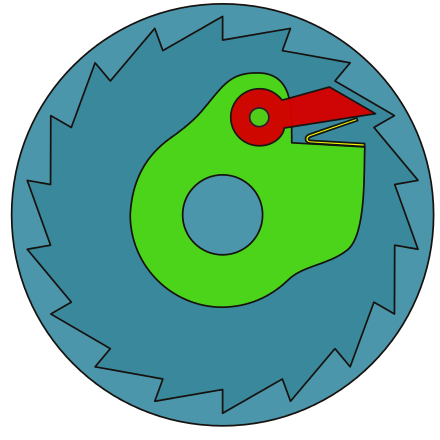
\includegraphics[width=.5\textwidth]{Figures/Freewheel.png}
  \caption{\label{fig:Freewheel}Diagram of a freewheel mechanism.}
\end{figure}

\indent\indent To overcome these operational challenges a set of mechanical freewheels and diodes will have to be placed into the mechanical rotational system and the circuits, respectively. The freewheel, like the one shown in [Fig. ~\ref{fig:Freewheel}], will allow powered rotation in one direction and free rotation in the other. The same design is implemented in bicycles and allows the move forward when pedaling forward but not brake or move backwards when pedaling in the opposite direction, also known as freewheeling. The diodes in the circuit allow for current to only travel in one direction. As a safety precaution they will be put in place into the circuit to prevent the back flow of any current should the motors rotate in the direction opposite of their intended use.

\subsubsection{Reel Motor}

\indent\indent The design of the reel motor is driven by the weight of the aeroshell. The aeroshell produces a high torque on the reel. To reel it up the motor must be able to meet this requirement. For previously discussed reasons a brushless DC motor was chosen. At peak efficiency these motors operate at a high rpm. Since this application requires torque over rpm gearing down is necessary. This is achieved through a worm drive gear reducer. The reducer chosen has a gear ratio of 20:1. The high rpm input of the motor is turned into a slower rpm, but higher torque output from the gear reducer. The gear reducer has a maximum torque output of $371.5 Nm$. A freewheel bearing will be used to prevent the shaft from transmitting power during release of the aeroshell.

\subsubsection{Release Motor}

\indent\indent The requirements of the release motor are determined by (1) the maximum angular velocity and acceleration needed to feed the tether out at a rate so that its linear velocity matches or exceeds the free fall velocities of the aeroshell and (2) the torque required to pull the tether off of the spool, which is dependent on the moment of inertia of the tether/reel system. During release, the tether is continually being pulled from the reel, thus making the moment of inertia of the system a dynamic value. These values have been calculated and are detailed in \ref{UnitReelDesignAnalysis}. From these calculations we determined the appropriate force necessary to remove the tether from the spool at a rate that would match the free fall of the aeroshell and thus ensure proper microgravity conditions. When paired with the geometries of the release disks are group was then able to determine the exact requirements of the release motor, which are detailed in \ref{ReleaseMotorDesignAnalysis}.

The design of the controls system for the release motor centered around making use of the pulse-width-modulation signal output from the Raspberry Pi computer on board. In combination with a dedicated motor controller we decided that this would be enough to precisely control the motors through whatever velocity profiles we designed. 

Original power systems concepts centered around the use of a single, robust power delivery system. Ultimately our group chose to split up the power delivery systems. Therefore, the release motor was design to have it's own power source of 12 volt DC batteries wired in series separate from the power sources driving the other electrically controlled subsystems. 

The physical mechanism that exists between the actual motor and tether is derived from the design of the previous iteration of this project. Two release disks, like the one shown in [Fig. ~\ref{fig:ReleaseDisk1}] will be fixed by their axis of rotation to the TUMBR unit. One of the release disks will be rigidly fixed to the rotation shaft of the release motor while the other release disk will be able to rotate freely. The two disks will be placed coplanar and sufficiently close enough to hug the tether as shown in the diagram. The edges of the release disks (i.e. the parts making contact with the tether), will be sufficiently rough enough to achieve a coefficient of friction necessary to grip the tether and pull it with the required forces. The friction force acting on the tether is the product of the compressive force, or normal force, resulting from the compression of the two disks on the tether and the coefficient of friction. The compressive force will be driven by the force requirements as outlined in \ref{ReleaseMotorDesignAnalysis}.

\begin{figure}[H]
  \centering
  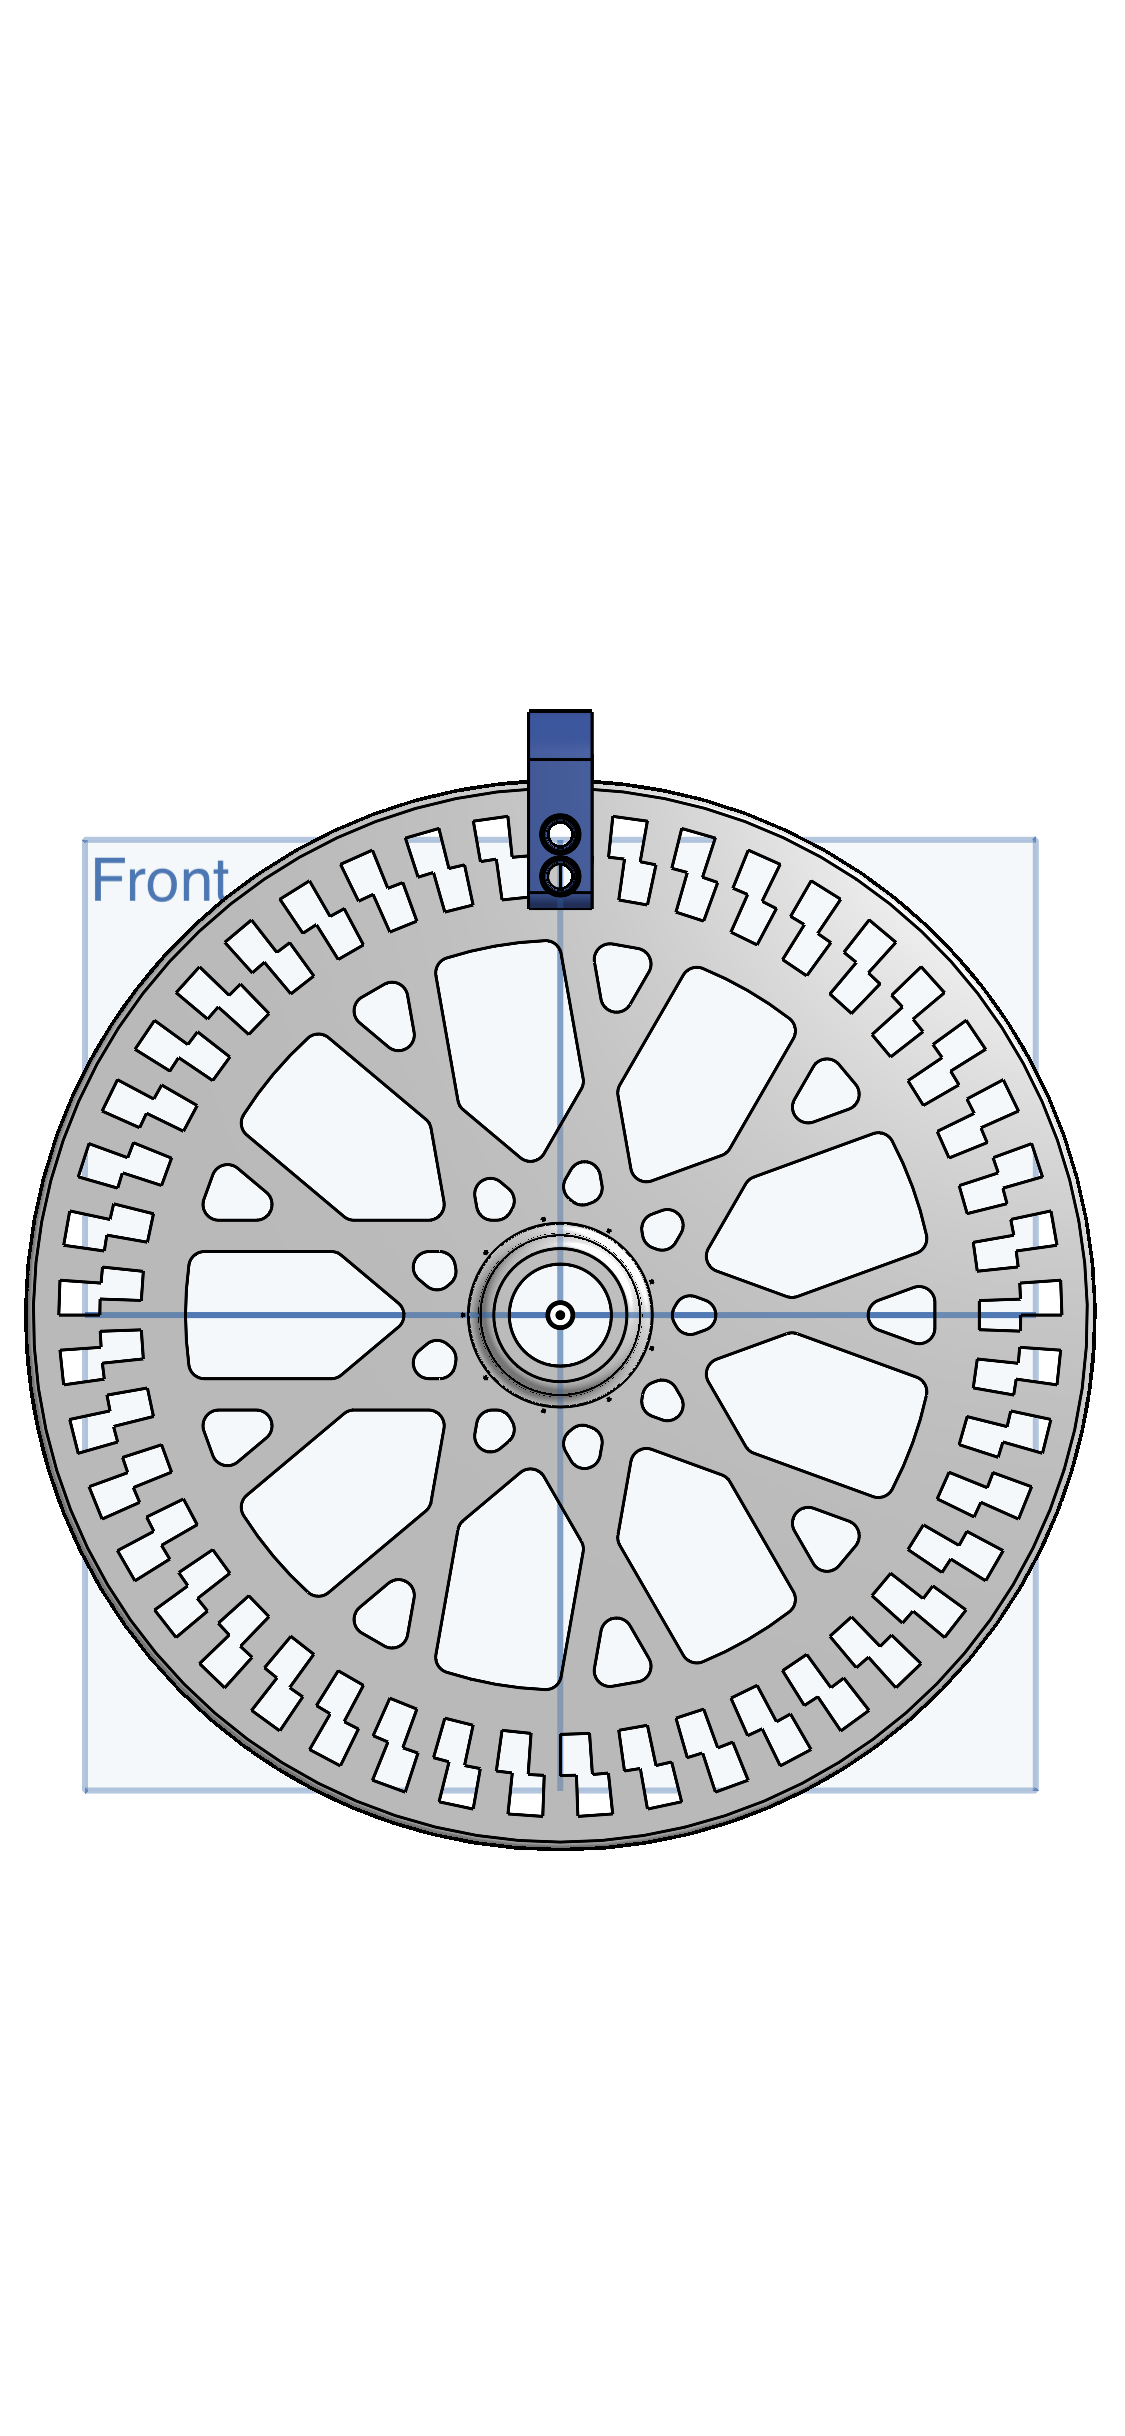
\includegraphics[width=.5\textwidth]{Figures/ReleaseDisk1.png}
  \caption{\label{fig:ReleaseDisk1}A CAD model of one of the release disks.}
\end{figure}

\subsubsection{Power}

\indent\indent To power the varies electrical components, our group decided to utilize over half a dozen lead-acid 12 volt DC batteries, wired in series to create the desired voltages need to power the various subsystems. Original concepts centered around the use of a single battery pack from which all power would be derived. However, to keep the design simple and to reduce the risk of total system failure the power system was split up between a 48 volt battery pack and a 24 volt battery pack. 

% ---------------------------------------------------------

\subsection{Controls \& Instrumentation}

%%\begingroup
%%\let\clearpage\relax
%%\include{Controls/controls_sys_concept_dev}
%%\endgroup
\input{Controls/controls_sys_concept_dev}

% ---------------------------------------------------------
% ---------------------------------------------------------
% ---------------------------------------------------------

\section{Design Analysis}

\begin{comment}

Introduce the methodology and analyses used in coming up with well-defined structure for the selected concept and major results. If the methodology is based on prior published work, cite the reference instead, with additional appropriate comments.

Examples of analysis techniques include:
•	Technical/mathematical modeling
•	Simulation
•	Quick prototype and experimentation

Present system and sub-system specifications used in your final design.

\end{comment}



\subsection{Aeroshell}

\subsubsection{Aeroshell}

\indent\indent The aeroshell is the part of the system that houses the payload. The payload will contain a middeck locker, which is where the actual microgravity experiment will be placed. The aeorshell will be attached to the TUMBR system via tether and will also house all the corresponding electronics. The aeroshell and internal structure both utilized the method of creating a model in SolidWorks and analyzing the model with ANSYS. Component-level testing was completed on the aeroshell and key connection areas for the internal structure. Proper materials have been chosen and applied for analysis with materials subject to change due to manufacturing stock, continuation of production, or change to an alternate material. With this in mind, the aeroshell system must be strong and rigid enough to endure the forces experienced from multiple high-speed drops, without experiencing any modes of failure such as corrosion, thermal shock, plastic deformation, and other modes of failure relating to the environment.

\indent\indent The aeroshell provides an aerodynamic and protective outershell for the middeck locker, electrical/data collecting components, and internal structure. Please refer to the Preliminary Design Review (PDR) report on the selection process for the airfoil used for the aeroshell. From this selection process, the aeroshell was modeled in SolidWorks by utilizing the revolve and shell features to create a 3D model. 

\subsubsection*{Computational Fluid Dynamics}
\indent\indent The analysis was completed using ANSYS Fluent, Static Structural, Thermal, and Vibration. Fluent was used for Computational Fluid Dynamics (CFD) to determine the drag force, pressure distribution, drag coefficient, and the reaction of fluid over the aeroshell (skin coefficient). This procedure was done by testing at sea-level and stratospheric conditions to see the effects of different conditions on the aeroshell. The model used for this analysis was SST k-omega and the changes to the default settings can be seen in [Table ~\ref{tab:cfdprojectschematic}].

\begin{table}[H]
\caption{\label{tab:cfdprojectschematic}CFD sea-level and stratosphere parameter differences.}
\centering
\resizebox{\textwidth}{!}{%
\begin{tabular}{|P{4cm}|P{8cm}|} 
\hline
 Setup Tree & Changes   \\\hline

Model & SST k-omega  \\ \hline
Materials: Air  & Strato: $\rho$ = 0.018 $kg/m^{3}$, $\nu$ = $1.485 \times 10^{-5}$ kg/m-s  \\ \hline
Boundary Conditions: inlet &  Sea-level: 19.42 m/s, Strato: [Table~\ref{tab:cfdvelocity}] \\ \hline
Methods: S.D. &  Second Order Upwind (all that apply) \\ \hline
Report Definitions & Drag force and $C_d$  \\ \hline
Initialization &  Standard Initialization  \\ \hline
Run Calculation &  1000 iterations  \\ \hline

\end{tabular}}
\end{table}

\indent\indent The table outlines any changes for sea-level and stratosphere conditions, but sea-level was mostly left to default. The boundary condition inlet velocity speed was set to $242.85 \sfrac{m}{s}$ with a $15 \sfrac{m}{s}$ cross wind speed. For the purpose of evaluating the max forces the aeroshell will experience, the velocity chosen was the terminal velocity of the aeroshell. The results pertain to the terminal velocity speed and below shows the relationship between the drag force over time [Fig. ~\ref{fig:dragforce}]. The velocity of the aeroshell was calculated at increments of 5 seconds and all with a crosswind of $15 \sfrac{m}{s}$ due to stratosphere conditions [Table ~\ref{tab:cfdvelocity}].

\begin{figure}[H]
  \centering
  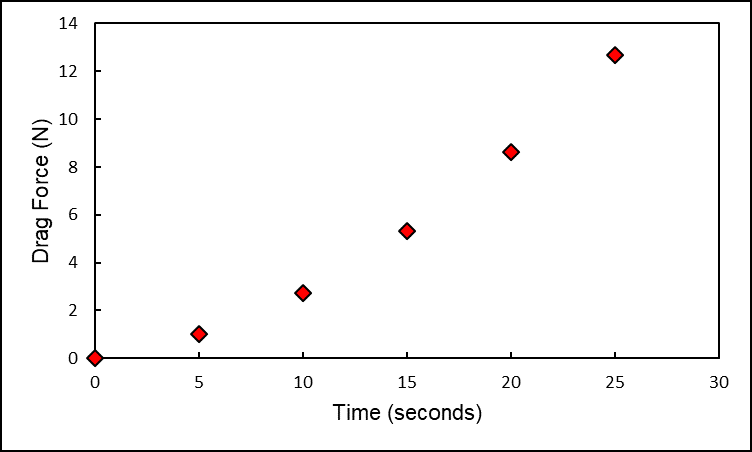
\includegraphics[width=0.7\textwidth]{Aeroshell/drag_relation.png}
  \caption{\label{fig:dragforce}Drag force over time.}
\end{figure}

\begin{table}[H]
\caption{\label{tab:cfdvelocity}Drag force and drag coefficient values from 0 – 25 seconds.}
\centering
\resizebox{\textwidth}{!}{%
\begin{tabular}{|P{2cm}|P{2cm}|P{3cm}|P{5cm}|P{4cm}|P{4cm}|} 
\hline
 Time (sec) & $C_d$ & Drag Force (N) & Aeroshell Velocity (m/s) & Wind Velocity (m/s) & Total Velocity (m/s)  \\\hline

0 & 0 & 0 & 0 & 0 & 0  \\ \hline
5 & 0.04407 & 1.0248 & 48.57 & 15 & 50.83  \\ \hline
10 & 0.03137 & 2.7279 & 97.14 & 15 & 98.29  \\ \hline
15 & 0.02749 & 5.3092 & 145.71 & 15 & 146.48  \\ \hline
20 & 0.02530 & 8.6450 & 194.28 & 15 & 194.86  \\ \hline
25 & 0.02377 & 12.6656 & 242.85 & 15 & 243.31  \\ \hline

\end{tabular}}
\end{table}

\indent\indent Another important aspect of the results from the E838 Hydrofoil CFD testing was the pressure contour around the aeroshell. For a symmetrical airfoil and successful flight, the center of pressure would need to be above the center gravity when falling. This can be seen in [Fig. ~\ref{fig:pressurecontour}] and [Fig. ~\ref{fig:cpcg}].

\begin{figure}[H]
  \centering
  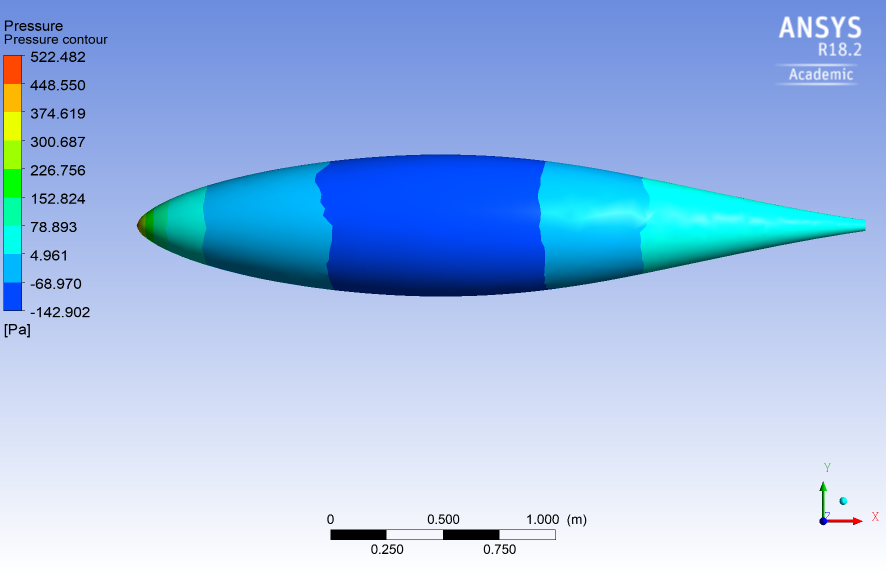
\includegraphics[width=0.8\textwidth]{Aeroshell/Pressure_contour.png}
  \caption{\label{fig:pressurecontour}Pressure contour over E838 Hydrofoil.}
\end{figure}

\begin{figure}[H]
	\centering
    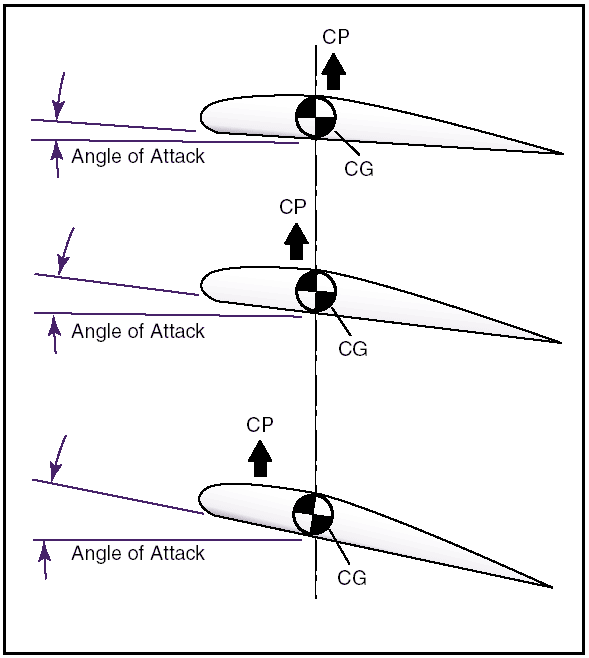
\includegraphics[width=0.55\textwidth]{Aeroshell/CP_angle_of_attack.png}
    \caption{\label{fig:cpcg}$C_p$ and $C_g$ relationship for symmetrical airfoil.}
\end{figure}

\subsubsection*{Static Structural}
\indent\indent To see if the carbon fiber outer shell can withstand the amount of force, finite element analysis (FEA) was performed to see the total deformation. Using the properties of carbon fiber and information from the CFD analysis, two evenly distributed forces that totaled $12.67 N$ was applied to the outer shell. The results show that the carbon fiber shell can withstand the force applied and it would move very little and these results correlate to the vibration analysis below [Fig. ~\ref{fig:deformation}].

\begin{figure}[H]
	\centering
    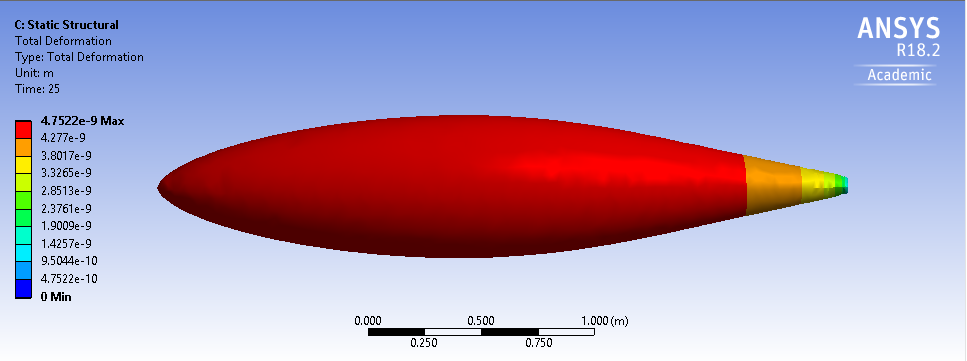
\includegraphics[width=0.8\textwidth]{Aeroshell/deform.PNG}
    \caption{\label{fig:deformation}Deformation of E838 Hydrofoil at terminal velocity.}
\end{figure}

\subsubsection*{Thermal}
\indent\indent The goal was to determine the temperature distribution that the aeroshell would experience during flight. The analysis was done at terminal velocity of $242.85 \sfrac{m}{s}$ with no cross wind. The analysis was run with an ideal gas constant and not the density of the stratospheric air due to error while running the program. The setup was very similar to the previous 3D CFD analysis, but the energy equation was turned on to add temperature parameters. The temperature around the airfoil was set to -46°C (226 K). The results show that towards the middle and trailing edge of the aeroshell it would receive a temperature increase higher than anywhere else on the aeroshell [Fig. ~\ref{fig:totaltemp}] [Table ~\ref{tab:temptable}]. This should be taken into consideration when placing items within and around the aeroshell.

\begin{figure}[H]
\centering
\begin{subfigure}[b]{.5\textwidth}
  \centering
  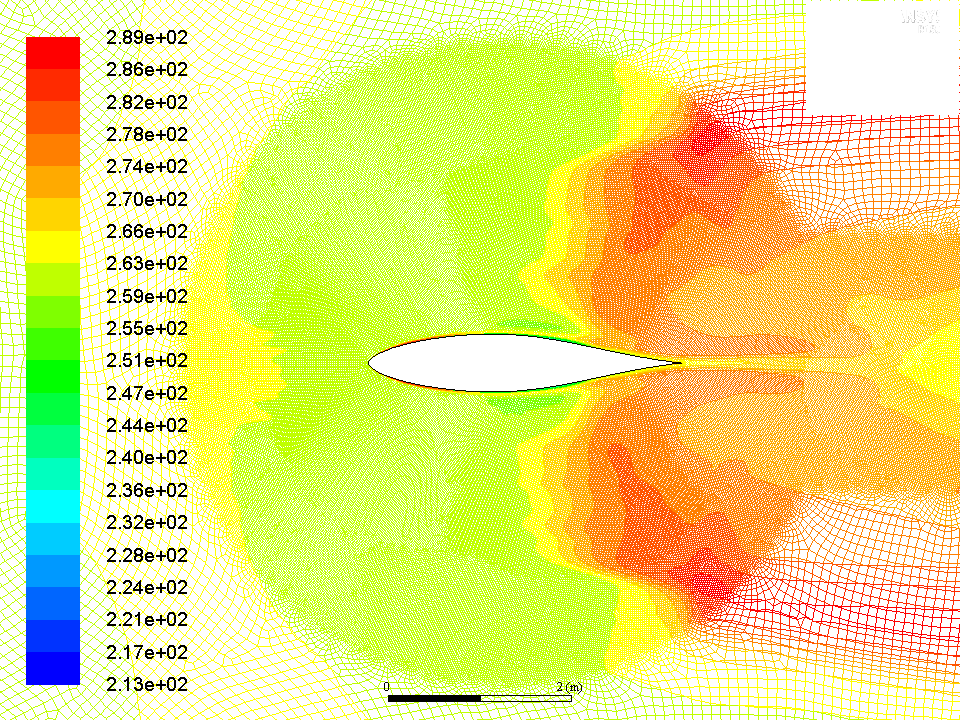
\includegraphics[width=0.9\textwidth]{Aeroshell/temp_contour.png}
  \caption{\label{fig:tempcontour}Temperature distribution at 25 seconds.}
\end{subfigure}%
\begin{subfigure}[b]{.5\textwidth}
	\centering
    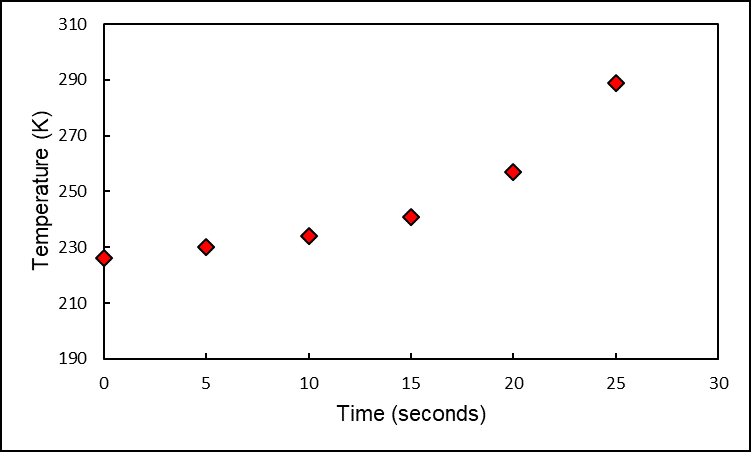
\includegraphics[width=0.9\linewidth]{Aeroshell/tempdistribution.png}
    \caption{\label{fig:tempdistribution}Temperature distribution throughout the flight.}
\end{subfigure}
\caption{\label{fig:totaltemp}Temperature distribution around E838 Hydrofoil}
\end{figure}

\begin{table}[H]
\caption{\label{tab:temptable}Maximum temperature values on aeroshell from 0 – 25 seconds.}
\centering
\resizebox{\textwidth}{!}{%
\begin{tabular}{|P{2cm}|P{5cm}|P{5cm}|} 
\hline
 Time (sec) & Aeroshell Velocity (m/s) & Max Temperature (K) \\\hline

 0 &   0.00 & 226  \\ \hline
 5 &  48.57 & 230  \\ \hline
10 &  97.14 & 234  \\ \hline
15 & 145.71 & 241  \\ \hline
20 & 194.28 & 257  \\ \hline
25 & 242.85 & 289  \\ \hline

\end{tabular}}
\end{table}

\subsubsection*{Vibration}
\indent\indent The vibration analysis was needed to understand the vibration environment during flight. Since the max drag force the aeroshell would experience was $12.67 N$, this was the testing point to see what the max vibration level would be at the terminal velocity. The goal was to see what impact would the vibration have on the payload and the quality of microgravity. This vibration analysis was also done with a solid body to try to simulate an internal structure within the outer shell. The random vibration analysis system would be the best choice for analyzing the aeroshell, but to produce a graph the project schematic had to change. Instead, using modal combined with a harmonic response analysis system produced a frequency vs. amplitude graph.

\indent\indent The two system analysis were linked by the engineering data, geometry, and model. A fixed support was created within the modal and harmonic response section in Mechanical. This was done to simulate the attachment of the tether to the aeroshell/internal structure combination. In the harmonic response section, a force of $12.67 N$ was applied at the nose of the aeroshell and the analysis setting’s max frequency was changed to $1.25 \times 10^6Hz$. This results of the vibration analysis showed that little vibration would occur, which would not severely disrupt the payload and quality of microgravity [Fig. ~\ref{fig:vibration}].

\begin{figure}[H]
  \centering
  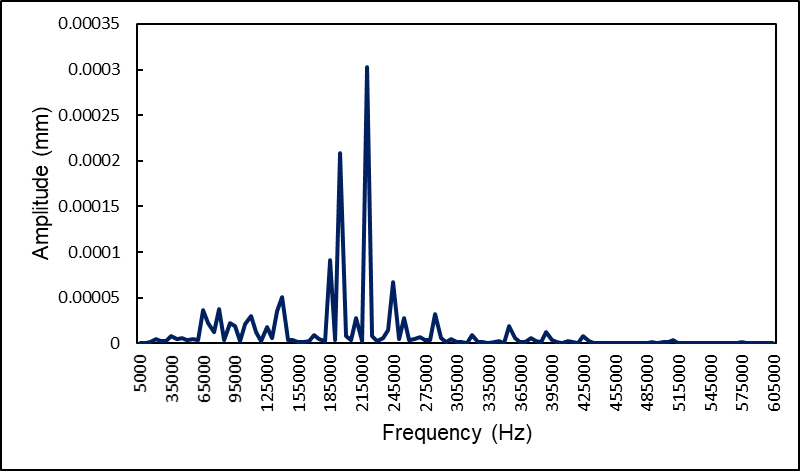
\includegraphics[width=0.8\textwidth]{Aeroshell/vibration.png}
  \caption{\label{fig:vibration}Vibration analysis of E838 Hydrofoil aeroshell.}
\end{figure}

\subsubsection*{Prototyping}

\begin{figure}[ht]
\centering
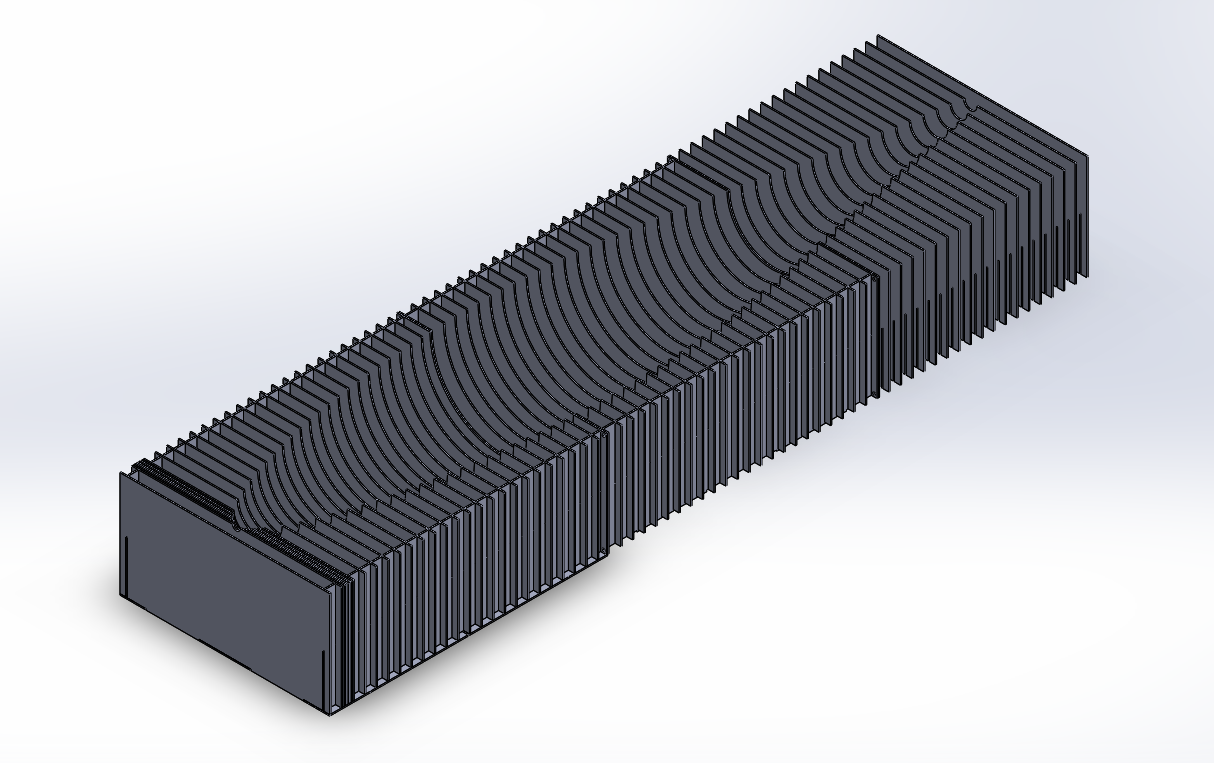
\includegraphics[width=0.8\textwidth]{Aeroshell/completedMold.PNG}
\caption{\label{fig:completedMold} Fully Assembled Mold.}
\end{figure}

\indent\indent Due to the complex geometry of the aeroshell and the material chosen, it was decided to produce the shell in halves (along the chord length) rather than other orientations. Prototyping the aeroshell halves will consist of making a twelve foot mold, built in a laser-cut lattice type structure, in three separate four foot sections [Fig. ~\ref{fig:completedMold}]. This segmented design is necessary for easy transportability and storage of the mold when and when not in use. The lattice will be entirely made of 0.25" medium density fiberboard (MDF) with the exception of the mold base which is 0.5" MDF. A total of seventy-eight boards will make up the cross sections of the airfoil geometry in two inch (centered) intervals, as any smaller gap would considerably increase the weight and cost of the mold. A slotted base and walls (all of identical material) will allow for easy assembly and alignment of the cross sections utilizing a finger joint type construction. As mentioned previously, a secondary 0.5" base will be used to ensure alignment of the four foot sections in addition to guiding dowel pins to provide added rigidity to the overall construction [Fig. ~\ref{fig:Section_Joint}].

\begin{figure}[H]
  \centering
  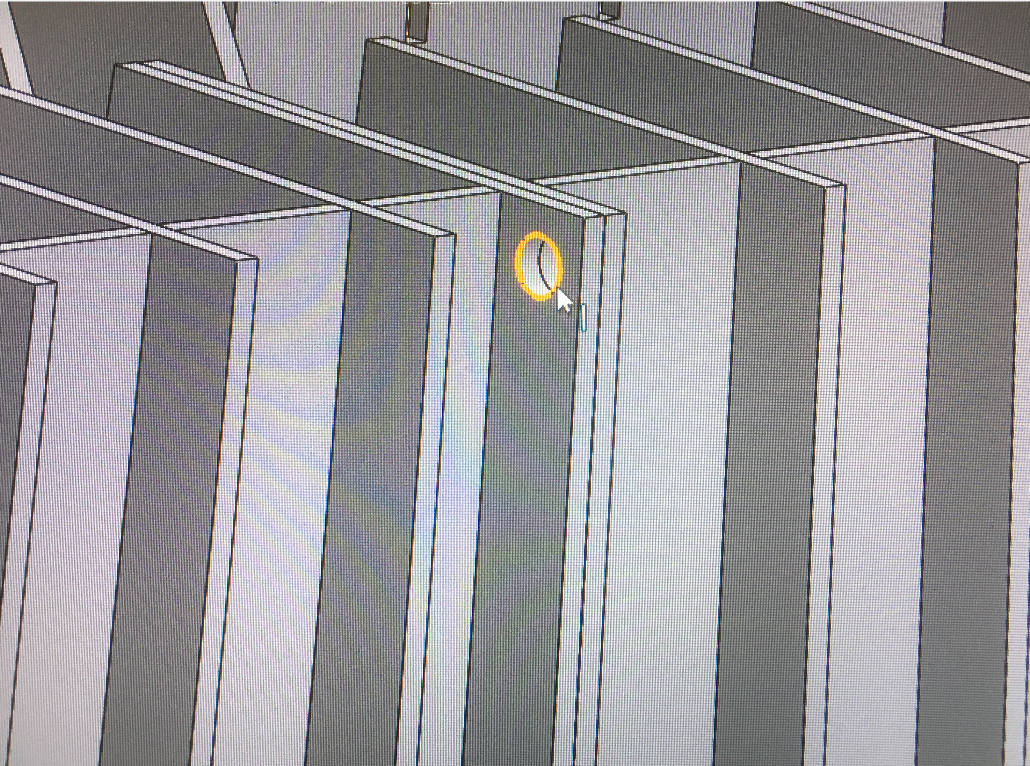
\includegraphics[width=.3\textwidth]{Figures/Section_Joint.PNG}
  \caption{\label{fig:Section_Joint} Mold Section Joints}
\end{figure}

\indent\indent Next, the gaps between the cross-section pieces will be filled with high density expanding foam that will serve as filler right to the top of the cross-section boards. The excess foam will then be sanded down to the very rough geometry of the desired shell before proceeding to the next step. Next, multi-purpose Bondo\texttrademark\ will be utilized as the secondary rough shaping of the shell, filling in the gaps between the boards and the foam to provide a roughly uniform surface. The bondo will then be sanded through the grits up through 220 before proceeding to spray Duratec\texttrademark\ sanding primer. This process further reduces surface roughness. Bondo will again be used to fill in low spots and build up material where needed before resanding and respraying the sanding primer. The previous step will be repeated until a smooth, uniform surface is achieved. Finally, the sanding primer will be mixed in a 1:1 ratio with a high gloss additive and sprayed onto the mold to produce a very fine, high gloss surface from which to mold from. A resin-infusion approach to carbon fiber manufacturing will then be taken to complete the molding process. The shell halves will be later joined via machined contour mounts to the internal structure before trimming off the excess mold material. This way the maximum material is removed while still preserving the closest interface possible between the two aeroshell halves. 

\indent\indent To test the functionality of the aeroshell faring, the assembly will be scale tested in a wind tunnel in order to extrapolate results as well as the full prototype being dropped from a substantial height to ensure proper aerodynamic stability in acordance to the aforementioned micro-gravity test requirements.

\subsubsection{Internal Structure}

\indent\indent The internal structure's primary constraints are the internal volume of the aeroshell and mass, to keep the total system under the 400 kg mass budget. To keep the aeroshell cross sectional area minimal, the internal structure was designed in SolidWorks to use the volume between the rectangular middeck locker and circular aeroshell, such that the largest diameter is the customers payload space. The primary structure material was chosen to be extruded 8020 aluminum for weight, ease of assembly and manufacturing, with mounting plates made of aluminum and carbon fiber to save weight. The internal structure has plenty of free space to mount electronics for environmental sensors and communication with the platform, and also has room to possibly mount a propulsion system to counter drag force and attain microgravity in future iterations of this project. The selection of 8020 as the main structure components allows for easy replacement of parts and also modularity for specific flight circumstances as needed, such as additional mounting points or additional electronics for the platform or to support an experiment.

\indent\indent The recovery tether attaches to the internal structure for strength and simplicity purposes. The structure, being made of aluminum, has isotropic properties so it is able to be more easily analyzed, requires less additional components to implement which saves mass, and eliminates a possible single point of failure by spreading the connection to 4 individual points. This tether attachment method is composed of 4 eye nuts connected to the top of the internal structure with 5/16” bolts passing through two parallel 8020 beams. This disperses the load across 4 different points, reducing the strength needed by each point. This method adds minimal additional weight for the hardware needed over a design that attaches to the aeroshell first. This method will need heavy lifting hooks, capable of locking to prevent accidental disconnection and also swiveling to prevent twisting the tether during drops.

\subsubsection*{Static Structural - Component Level Testing}
\indent\indent With the tether attached to the internal structure at the top, the greatest forces will be experienced at this point as the greatest mass is being decelerated during braking. Assuming a payload up to 27 kg, the internal structure and aeroshell fully loaded mass is currently approximated to be 85 kg (154 lbs.). If braking is ramped up to 5 g’s of deceleration, the tether would experience about 935 lbs. of force. With some limitations to a full internal structure analysis, a component level analysis was conducted to connection points throughout the internal structure. Parts repeat throughout the structure, so the part that would experience the most force and fatigue over time was tested for worst case scenario. Therefore, the other similar parts would pass under this testing process.

\paragraph{Oval Eye Nut Analysis} Analyzing the connection points, using 5/16-18 eye nuts connected to the frame with a matching thread bolt through the 8020 beam the force required to reach yield of the bolt is 4542.6 lbs. Which compared to the expected max force on the tether of 770 lbs. gives a factor of safety of 5.9 for a single bolt connection. Dividing the load across 4 connection points further increases it such that the eye nut and bolt connection should not be a point of failure. These bolts pass through series 40 8020 aluminum beams with washers on the opposing side to disperse the load to the entire beam face. Each remaining connection point in the frame is secured with two of the same bolts passing through 8020 beams, so no point farther down the structure should fail under expected braking loads.

\subsection{TUMBR}

\subsubsection{Tether}

\indent\indent The tether being used for this prototype is a specialized fiber which is sourced from one manufacturer, Honeywell. Honeywell supplies the raw fiber which can be sent to cordage companies which spin the fibers into the tether specified. Mazzella Companies provided the service of taking the raw material and making it into a usable product. The properties of the fiber was provided by the cordage manufacturer and can be found in the CDR Data Packet. The Spectra fiber was chosen due to the product keeping its shape integrity throughout the un-spooling process throughout the flight. It is important for the tether to keep its shape throughout the un-spooling process, so that the tether guide can have a constant and consistent shape passing through it. Below contains a list of features that Spectra 12 Strand tether provides toward the project.

\indent\indent Because of the heritage and regular use of this material in industry for high force applications our group felt confident that the tether would be able to comfortably tolerate the static and dynamic forces encountered throughout flight. It was calculated that a nominal tension of $3981 N$ will be applied throughout the tether during the braking process. According to the 12 Strand Spectra data sheet located in the CDR Data Packet, the tensile strength for $1/4 in$ Spectra tether is 2.4 metric tonnes, which corresponds to approximately $23,500 N$, well above the forces we expect to encounter. 

\textbf{Features \& Benefits:}

\begin{itemize}[noitemsep]
  \item Very low stretch
  \item Very high strength
  \item Soft hand
  \item Torque free
  \item Easy splicing
  \item Floats
\end{itemize}

\subsubsection*{Prototyping}

\indent\indent Prototyping the tether consists of no alteration to the size, but to the length of the tether to sea-level conditions. The length of the tether would be cut down to accommodate sea-level testing. This would only be the case with the approval from officials at a qualified testing site with proper supervision and approved test plan procedure.

\indent\indent The full-scale of the tether provides challenges when trying to test the product to ensure that it will perform properly during flight. Testing of the tether would consist of smaller sections with multiple testing coupons. Testing would consist of elongation/torque, abrasion, water resistance, and climate (i.e. temperature) testing. Each coupon would undergo each test to receive the full effect and worst case scenario. If the coupon testing pass the worst case scenario then no further testing would be required unless otherwise noted by the FAA and their requirements.

\subsubsection{Tether Guide}

\indent\indent When reeling up the aeroshell it is important for the tether to be wound evenly along the reel. Two methods to achieve this were researched including the use of a traverse roll mechanism and a rolling ring drive. It was ultimately decided to use the rolling ring drive depicted in [Fig. ~\ref{fig:RollingRingDrive}] as it would be simpler to implement and control. This mechanism utilizes roller bearings in order to change rotational shaft motion into constant traverse movement. The drive is attached to a rotating shaft and the bearings press against it to create friction and move the drive forward. The speed at which the box moves back and forth is mechanically set. The distance it traverses is also set prior to use and in this application is six inches. 

\begin{figure}[H]
  \centering
  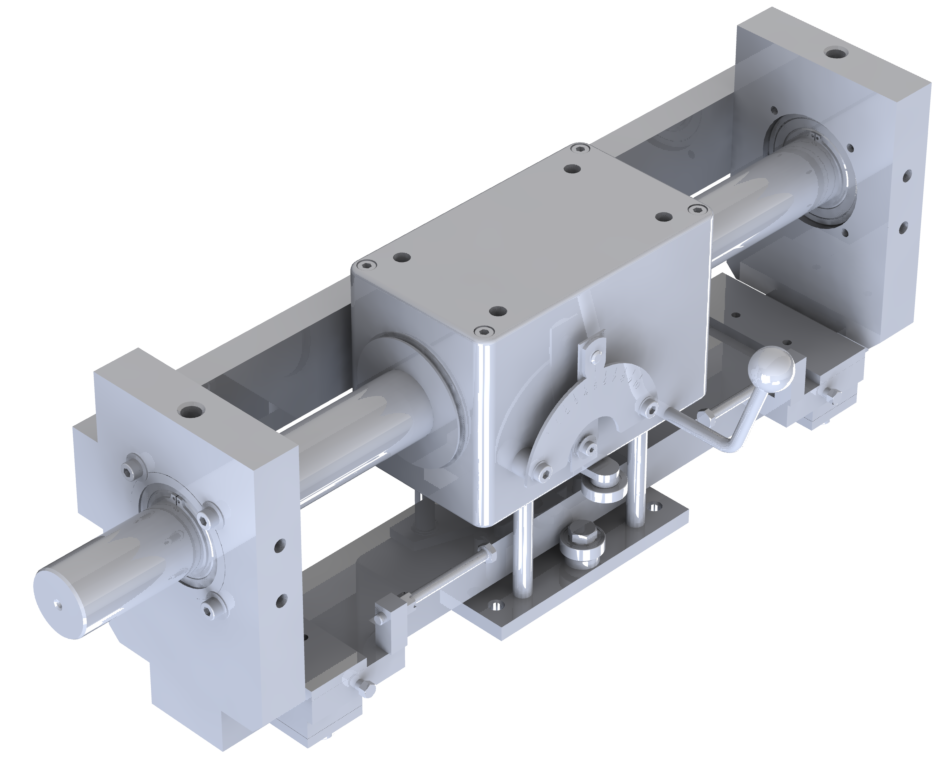
\includegraphics[width=.7\textwidth]{Figures/RollingRingDrive.png}
  \caption{\label{fig:RollingRingDrive}CAD render of the rolling ring drive.}
\end{figure}

\subsubsection{Brakes}

\indent\indent After researching into many different types of braking systems, such as drum or electromagnetic, our group agreed on the finale design of using dual disk brakes. The shaft will have a set of disk brakes which include brake pads, rotors, rotor mounts, calipers, a master cylinder, a linear actuator. The rotor mounts will be welded onto the shaft which also houses the spool and tether and will provide a mounting point for the brake rotors. The brake calipers will have a separate mount which will be bolted to the main surface of the entire unit allowing the calipers to have a sturdy connection point. The master cylinder will also be mounted on the main surface of the unit with brake lines leading to the two calipers. The linear actuator will be located close to the master cylinder in order to apply a pressure into the master cylinder. A CAD model of the subsystem will accurately represent the layout of the braking subsystem.

Physical characteristics that the braking subsystem would endure were modeled and simulated in Ansys.  Using the fundamental engineering principals of thermodynamics, heat transfer, machine design, and solid mechanics the boundary conditions for the simulation could be set. Boundary conditions including but not limited to thermal conductivity of the material, heat transfer coefficient of the fluid surrounding the brake, forces and torques applied on the brakes, and thermal/elastic properties of the materials. These are the boundary conditions and fundamental knowledge which are being used currently to run a simulation on the system dynamics. 

The brakes will engage when a successful nine seconds of microgravity has passed. The aeroshell will experience $3 g's$ of deceleration, which is approximately $30 m/s^2$. Using this deceleration and a conservative weight of $981 N$, the tension acting on the tether can be calculated. The tension acting upwards on the tether will be the same force which the shaft, which the braking system is connected to, will experience in a downwards direction. The moment of inertia of the shaft and all of the connected components was calculated to be $0.0772 kg*m^2$, and the rotational acceleration of the shaft was calculated to be $200 rad/s^2$ using the linear deceleration and radius of the tether at the nine second mark. The braking force was then calculated by equating the product of the moment of inertia and radial acceleration to the sum of the forces acting on the system. This yields that the braking force needed for a nine second drop would be 8,878 Newtons. The amount of heat produced by the braking system will be approximately equal to the amount of energy built up in the system, since the brakes will be the only force acting on the aeroshell and shaft to slow them down. The justification for this simulation has not been experimentally confirmed yet. It is in future plans to test the system and experimentally validate the model and simulation.

Inefficiencies in bearings and fluid dynamics, such as friction, has been neglected in the calculations and simulations run, however we are confident that the dynamics of the system have been accurately modeled and will be experimentally validated. The experiment all data will then be compared to the modeled data which will be compared to the expected performance of the system.

\subsubsection{Unit and Reel} \label{UnitReelDesignAnalysis}

\indent\indent After conducting trade studies for a variety of spool and reel dimensions throughout Senior Design 1, our group converged onto a final design. As shown in [Fig. ~\ref{fig:TUMBRSpoolFrame}], a shaft with a thickness of 1.5 inches will have a rotor mount as well as two disks making up the tether housing walls welded perpendicular to its' central axis. The shaft itself will be supported via two 80/20 aluminum structured fixed on either side and connected via a high-speed mounted bearing. The two tether housing walls will be spaced 6 inches apart and contain the tether. A rotor mount will be welded down the shaft and will provide a mounting point for the brake disks. The shaft will be mounted to two bearings, allowing the shaft to rotate as the tether is released and reeled back up. Our group has designed a CAD model of our system, which accurately captures the dimensions the system will be manufactured to. Physical characteristics of the system, such as the moment of inertia of the steel shaft, were calculated using SolidWorks and OnShape and used standard material properties of steel. To ensure that the tether housing walls and rotor mounts are welded perfectly perpendicular with respect to the central axis of the shaft, we modified our design so that the diameter of the piece was slightly decreased at the point of mounting. This will allow either piece to easily fit onto the shaft but will provide a surface to be fitted and welded to.

\begin{figure}[ht]
 \centering
 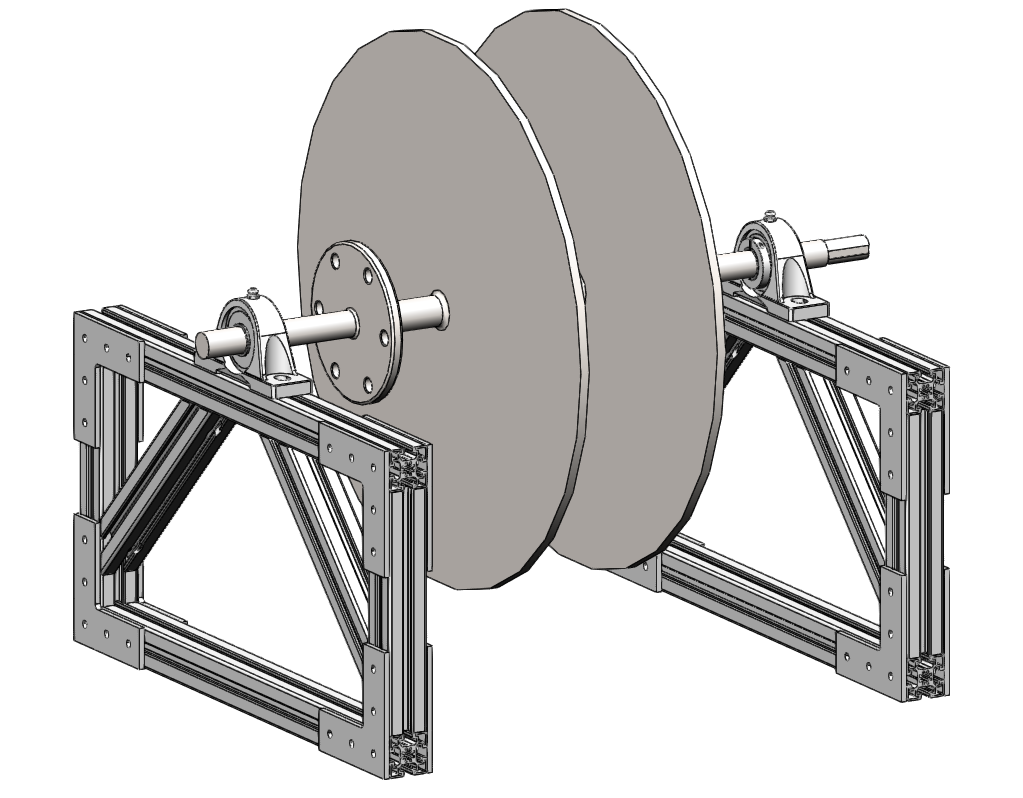
\includegraphics[width=0.8\textwidth]{TUMBR/SpoolFrame.PNG}
 \caption{\label{fig:TUMBRSpoolFrame} CAD diagram detailing the reel system, which includes the shaft, tether housing walls, brake rotor mount, high-speed bearings, and supporting walls.}
\end{figure}

\indent\indent Throughout the test the tether will be repeatedly un-spooled, decelerated, and then reeled back up. Enabling this motion are two electric motors and a braking system. To properly characterize the performance required from these components, a complete analysis of the dynamics of this system and how they are expected to change with time has been calculated. 

\indent\indent The dynamics of the reel system are dependent upon the dimensions of the entire subsystem, which change depending on how much tether is wrapped around the spool at any moment in time. To determine these parameters we first assumed a constant thickness of the tether of about 0.25 inches. This assumption is justified due to a key property of the tether we selected; it has very little elongation and changes in dimension when under a load. Assuming the tether can be cleanly wrapped every time, we calculated the thickness of the tether as it's wrapped around the spool as a function of the total length of the tether. Our group incorporated a tether guide into our design, which is a system capable of cleanly wrapping a line of tether or cord around a spool and is commonly used in industry on various types of winches. With the entire $670+ m$ of the tether wrapped around the shaft there will be approximately 35 layers of tether that result in a diameter of approximately $18.5 in$. The total mass of the tether will be approximately $16.09 kg$ and have a maximum moment of inertia of $0.447 kg\times m^2$. The combined moment of inertia considering the tether, shaft, rotor mounts, etc. will be approximately $0.523 kg\times m^2$. These parameters of the system throughout the drop and thus the torque required to alter the motion of the system change as well. At time $0.1 s$ a maximum torque of $21.83 Nm$ will be required to accelerate the shaft and tether so that the tether is accelerated at $9.81 m/s^2$. When considering the radius from the central axis that the tether is being pulled from, this results in a required force (or tension in tether) or approximately $46.46 N$. At time $9 s$ a torque of approximately $9.866 Nm$ will be required to continue accelerating the shaft. Likewise, a force of $32.370 N$ is required to produce this torque. These results are described in completion in the CDR Data Packet and are summarized in  [Table ~\ref{tab:TL6inSpool}] and [Table ~\ref{tab:SpoolDynamics}]. Note, that the missing data in [Table ~\ref{tab:SpoolDynamics}] is a result of erroneous values produced from the abrupt change of diameter of the remaining wrapped tether. This is an artifact of the discrete input of tether diameter used for mathematically modeling the system in Excel and therefore the erroneous data is omitted to convey the smooth transitions we expect. 

\begin{table}[H]
\caption{\label{tab:TL6inSpool}Relationship between coil number, coil diameter, and tether length for 1/4 in diameter tether and 6 in spool.}
\centering
% You need as many of these as you have columns i.e 3 columns ==> {l|c|c}
% To control width of a box you must be "hack-y" and treat the cell as containing a paragraph i.e use P{width}
\resizebox{\textwidth}{!}{%
\begin{tabular}{|P{2.5cm}|P{2.5cm}|P{2.5cm}|P{2.5cm}|P{2.5cm}|P{2.5cm}|} 
\hline\hline
Coil \# & Diameter of Coil (in) & Length of Tether/Coil (in) & Length of Tether/Wrap (in) & Total Length of Tether (in)	& Total Length of Tether (m) \\\hline

0 & 0 & 0 & 0 & 0 & 0\\\hline
1 & 1.5 & 4.712 & 113.097 & 113.097 & 2.873\\\hline
2 & 2 & 6.283 & 150.796 & 263.894 & 6.703\\\hline
3 & 2.5 & 7.854 & 188.496 & 452.389 & 11.491\\\hline
… & … & … & … & … & …\\\hline
33 & 17.5 & 54.978 & 1319.469 & 23637.343 & 600.389\\\hline
34 & 18 & 56.549 & 1357.168 & 24994.511 & 634.861\\\hline
35 & 18.5 & 58.119 & 1394.867 & 26389.378 & 670.290\\\hline

\end{tabular}}
\end{table}

\begin{table}[H]
\caption{\label{tab:SpoolDynamics} Condensed dynamics of spool at key points of drop.}
\centering
% You need as many of these as you have columns i.e 3 columns ==> {l|c|c}
% To control width of a box you must be "hack-y" and treat the cell as containing a paragraph i.e use P{width}
\resizebox{\textwidth}{!}{%
\begin{tabular}{|P{2.5cm}|P{2.5cm}|P{2.5cm}|P{2.5cm}|P{2.5cm}|} 
\hline\hline
Time Step (s) & Angular Velocity (rpm) & Avg. Ang. Acceleration (rpm/s) & Torque (Nm) & Force Required (N)\\\hline

0.1 & 39.8717 & 398.7171 & 21.8330 & 46.4632\\\hline
0.2 & 79.7434 & 398.7171 & 21.8289 & 46.4544\\\hline
0.3 & 119.6151 & 398.7171 & 21.8221 & 6.4399\\\hline
… & … & … & … & …\\\hline
8.7 & 5133.8823 & 590.1014 & 10.3655 & 32.6471\\\hline
8.8 & 5192.8924 & 590.1014 & 10.2027 & 32.1346\\\hline
8.9 & 5470.7318 &  &  & \\\hline
9 & 5532.2007 & 614.6889 & 9.8664 & 32.3701\\\hline

\end{tabular}}
\end{table}

\indent\indent Given the complete dynamical modeling of the system, our group has also carried out a structural analysis of the shaft when it experiences its' maximum applied force and torque. This occurs during the deceleration period when the shaft experiences an applied torque from the brakes about its' central axis of rotation as well as an applied torque about the same axis resulting from the tension in the tether from the decelerating aeroshell. A linear force acting in the negative z-direction is also considered as a result from the tether under tension. 

\indent\indent Given the complete dynamical modeling of the system, our group has carried out structural analyses using SolidWorks FEA simulations. Approximations of some designs and lower resolution mesh is a comprise our group has made to produce the simulations using the software under a limited student license. The 80/20 aluminum frame shown in [Fig. ~\ref{fig:TUMBRSpoolFrame}] supports the weight of the shaft throughout the duration of the test. The expected load fluctuates depending on where the system is in the mission profile. For example, at the home position with the tether fully retracted, the 80/20 has to support the static weight of the shaft, tether, and aeroshell, which results in a mass of approximately $200 kg$. During braking, which the aeroshell is decelerating at an expected rate of $3 g's$, which results in a tension within the tether of approximately $4000 N$. Our group utilized 80/20's provided deflection calculator to determine the deflection that the horizontal beam supporting the load would experience, provided that there are no diagonal beams offering reinforcement. The generated report is displayed below in [Fig. ~\ref{fig:8020Deflection1}] and [Fig. ~\ref{fig:8020Deflection2}]. It was found that the maximum deflection at the center of loading will be about $0.0222 in$. When accounting for the two separate walls that will be supporting this load we can expect the deflection to be halved. 

The frames that the shaft is fixed to are designed to be mounted to a metal platform, which will itself be fixed to the stratospheric balloon that will provided the flight service for our vehicle. Using the previously discussed maximum force calculations encountered during the braking process, our team calculated the deflection for metal plates of various thicknesses. Ultimately we determined an optimum thickness of $1/4 in$ that balanced mass with strength. The SolidWorks simulations are shown below in [Fig. ~\ref{fig:Platedeflect}] where we found a maximum delfection of 0.745 in. 

\begin{figure}[ht]
 \centering
 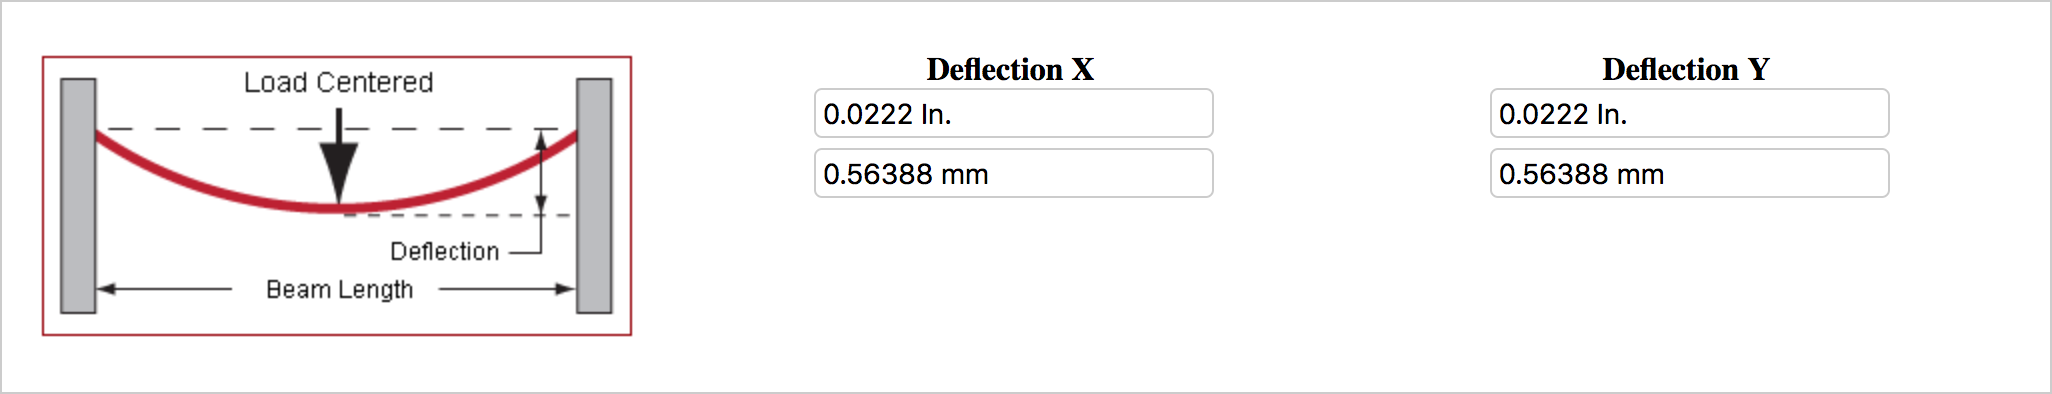
\includegraphics[width=1\textwidth]{TUMBR/8020Deflection1.png}
 \caption{\label{fig:8020Deflection1} The calculated deflection of a single beam of 8020 aluminum supported at both ends under maximum loading.}
\end{figure}

\begin{figure}[ht]
 \centering
 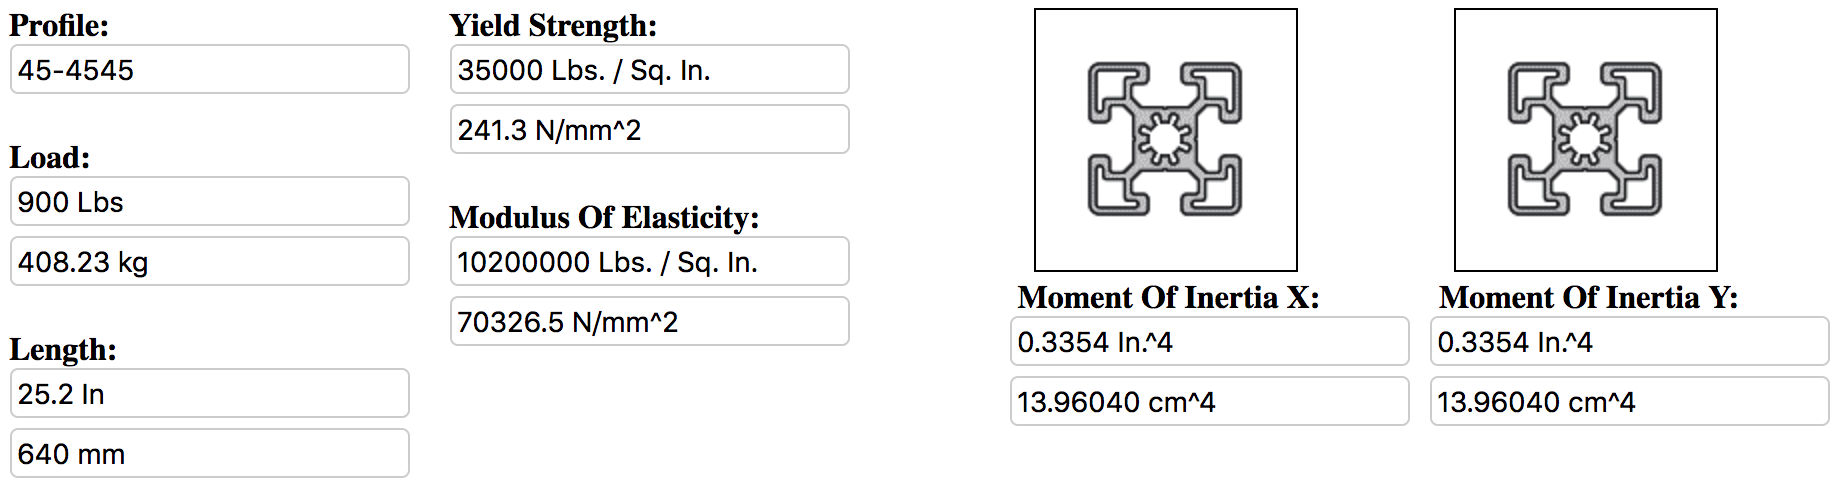
\includegraphics[width=1\textwidth]{TUMBR/8020Deflection2.png}
 \caption{\label{fig:8020Deflection2} Deflection parameters and 8020 aluminum beam material properties.}
\end{figure}

\begin{figure}[ht]
 \centering
 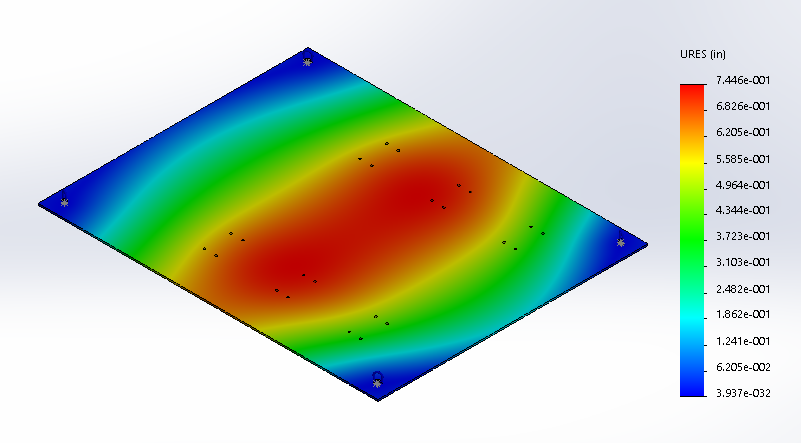
\includegraphics[width=1\textwidth]{TUMBR/Platedeflect.PNG}
 \caption{\label{fig:Platedeflect} Mounting plate deflection.}
\end{figure}

These calculations provides us with confidence that our design will be robust enough to endure the extreme loading this structure and frame will experience.

\indent\indent Our group is confident that we have accurately captured the dynamics of the system, save for a key uncertainty mentioned above that will be experimentally validated. Unaccounted for are the inefficiencies of these system that are assumed to be negligible. For example, we are not considering the friction due to the bearings or the minute dimensional changes of the tether. Key principles to this modeling effort revolved around dynamics and solid mechanics of complex systems. The design is simple enough where we have been able to reasonably account for the expected effects of all components. The performance will be tested, as described in a later, and compared with model expectations.  

\subsubsection{Reel Motor}

\indent\indent The reel motor is responsible for returning the aeroshell back to the platform within a reasonable amount of time. Driving the design of the reel motor is the high torque required to lift the aeroshell. A roller attached to the platform will feed the tether back to the reel and eliminate variable torque as the tether is spooled.

\indent\indent Motors generally operate at a high rpm at peak efficiency. For this high torque application the rpm of the motor will need to be decreased while the torque output increases proportionally. This is achieved with a worm gear reducer. This multiplies the torque output by a factor of twenty. Maximum output for the gear reducer is $371.5 Nm$. This is more than enough power to lift the aeroshell. If any future projects need more torque the gear reducer will still hold up. A freewheel bearing attached to the shaft will ensure power is transmitted only while reeling up. The bearing can rotate freely during release. While reeling up the bearing catches on a mechanism and transmits power.

\subsubsection{Release Motor} \label{ReleaseMotorDesignAnalysis}

\indent\indent The release motor will ultimately provide the force necessary to release the tether from the spool ensuring there will be zero tension in the tether, thus allowing the aeroshell to achieve quality microgravity conditions. The output shaft of the release motor is connected to a belt and pulley system that provides a 2.9:1 gear reduction, allowing the motor to operate at near peak efficiency. This arrangement is suited only for the 2 second drop whereas a proposed 9 second drop would require the motor to max out on its angular velocity capabilities leaving no room for gear reduction i.e. a reduction in speed through gearing. The output shaft from the belt and pulley system will be fixed to a release disk. There will be two release disk; one receiving the applied torque from the motor and the other being free to rotate. The two disks are co-planar and between the tether is compressed. When rotating, the normal force acting on the tether combined with the friction will provide a friction force, characterized in \ref{UnitReelDesignAnalysis} and displayed in [Table ~\ref{tab:SpoolDynamics}, that will un-spool the tether. This system has been designed in the CAD software SolidWorks and is [Fig. ~\ref{fig:release_transmission}]. 


\begin{figure}[ht]
\centering
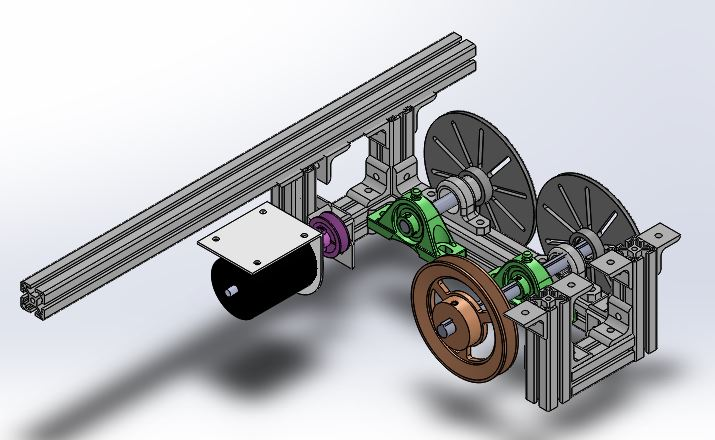
\includegraphics[width=0.8\textwidth]{Figures/release_transmission.PNG}
\caption{\label{fig:release_transmission} Isometric view of Release Motor Transmission System.}
\end{figure}


With the force required to achieve the desired velocity of the tether, the angular velocity of the release disks and the torque and power required from the motor has been calculated and is summarized in [Table ~\ref{tab:ReleaseDiskDynamics}]. Complete calculations may be found in the Milestone 6 Data Packet.  

\begin{table}[H]
\caption{\label{tab:ReleaseDiskDynamics} Condensed dynamics of release disk at key points of drop.}
\centering
% You need as many of these as you have columns i.e 3 columns ==> {l|c|c}
% To control width of a box you must be "hack-y" and treat the cell as containing a paragraph i.e use P{width}
\resizebox{\textwidth}{!}{%

\begin{tabular}{|P{2.5cm}|P{2.5cm}|P{2.5cm}|P{2.5cm}|P{2.5cm}|P{2.5cm}|P{2.5cm}|P{2.5cm}|P{2.5cm}|}
\hline\hline
Time Step & Linear Velocity (m/s) & Angular Velocity (rad/s) & Angular Velocity (rpm) & Avg. Ang. Acceleration (rad/s$^2$) & Avg. Ang. Acceleration (rpm/s) & Force Required (N) & Torque (Nm) & Power Required (W)\\\hline

0   & 0     & 0      & 0       & 0       & 0        & 0      & 0     & 0        \\\hline
0.1 & 0.981 & 11.036 & 105.387 & 110.361 & 1053.871 & 46.463 & 4.130 & 45.580   \\\hline
0.2	& 1.962 & 22.072 & 210.774 & 110.361 & 1053.871 & 46.454 & 4.129 & 91.143   \\\hline
0.3	& 2.943 & 33.108 & 316.161 & 110.361 & 1053.871 & 46.440 & 4.128 & 136.672  \\\hline
…   & …     & …      & …       & …       & …        & …      & …     & …        \\\hline
8.7 & 85.347 & 960.142 & 9168.678 & 110.361 & 1053.871 & 32.647 & 2.902 & 2786.333\\\hline
8.8 & 86.328 & 971.178 & 9274.065 & 110.361 & 1053.871 & 32.135 & 2.856 & 2774.115\\\hline
8.9 & 87.309 & 982.214 & 9379.453 & 110.361 & 1053.871 &        &       &         \\\hline
9.0 & 88.290 & 993.250 & 9484.840 & 110.361 & 1053.871 & 32.370 & 2.877 & 2857.955\\\hline
%It's fixed! Fuck yeah!

\end{tabular}}
\end{table}

It was found that at time $0.1 s$ a torque of $4.130 Nm$ would be required to produce an average angular acceleration of 110.361 $rad/s^2$. At the conclusion of the drop at time $9.0 s$ a torque of only $2.877 Nm$ will be required to produce an angular velocity of $9484.840 rpm$ in the release disks. 

Important assumptions our group made when modeling this system is that the release disks and tether will experience no slippage. This will be achieved with adequate compression between the two disks combined with a rubber coating to optimize friction. Our group has also not accounted for the minor inefficiencies of the system (e.g. friction of bearings) but expected these to be negligible. Inefficiencies of the belt and pulley system have considered and factored into the motor requirements. 

\subsubsection{Power}

\indent\indent The release motor will be powered via four Apex UB12220 12V 22AH batteries wired in series. This arrangement will provide approximately 48 VDC and will be capable of providing the 40 amps necessary to power the motor. Performance spec sheets have been thoroughly analyzed and extensive conversations with company engineers were had to ensure that the batteries would meet the performance requirements of our system. Because the release motor runs on such a short duty cycle and we expect to perform approximately half a dozen drops throughout any given flight, the batteries are modeled to have plenty of storage capacity for any given flight. Key aspects to understanding and modeling the power system revolve around electrical systems engineering.

% ---------------------------------------------------------
\subsection{Controls \& Instrumentation}

\input{Controls/controls_design_analysis}
% ---------------------------------------------------------

% ---------------------------------------------------------
% ---------------------------------------------------------
% ---------------------------------------------------------

\section{Final Design and Engineering Specifications}

\subsection{Aeroshell}

\subsubsection{Aeroshell}

\indent\indent The final design of the aeroshell consists of a revolved E838 Hydrofoil that is 11.22 ft. long and weighs approximately 12.74 kg. [Fig. ~\ref{fig:aeroshell}]. The aeroshell is being made out of carbon fiber to accommodate the internal structure, which will house the middeck locker. The aeroshell creates an aerodynamic and protective housing unit for the middeck locker to provide microgravity results through multiple drops. The aeroshell is manufactured in-house by a MDF board laser cut skeleton. The skeleton consists of 69 slats horizontally going from tip to tail and they are held together by 6 side and 6 floor slats. The spacing between the horizontal slats are filled with expanding foam and packing peanuts. The foam is then covered by BONDO that is sanded downed and buffed before placing the carbon fiber down to be manufactured by vacuum pressure. Each side of the aeroshell are manufactured out of 8 sheets of carbon fiber for structural strength. The two manufactured aeroshell sides will be held together by the internal structure through 8 mounting blocks that are attached to the internal structure and CNC machined out of aluminum.

\begin{figure}[H]
  \centering
  \includegraphics[width=0.8\textwidth]{Aeroshell/aeroshell.png}
  \caption{\label{fig:aeroshell}Manufactured aeroshell model rendering.}
\end{figure}

\subsubsection{Internal Structure}

The final design of the internal structure is made up of 16 8020 aluminum T-slot framing varying in 12, 16, and 20 inches in length, 8 CNC machined aluminum mounting blocks that are the connecting point between the aeroshell and internal structure, 4 oval eye nuts at the top of the structure that serve as the connection between the tether and internal structure/aeroshell, 4 plates that are distributed throughout the structure for structural integrity, and hardware to attach all the parts together. The hardware consists of bolts, nuts, l-brackets, and elbow brackets. The overall dimensions of the internal structure is 12.15 in. x 16.15 in. x 45.25 in. (l x w x h). The internal structure will house the middeck locker and will take majority of the braking force. This structure is a new addition from the previous iteration and can be seen in  below

\begin{figure}[H]
  \centering
  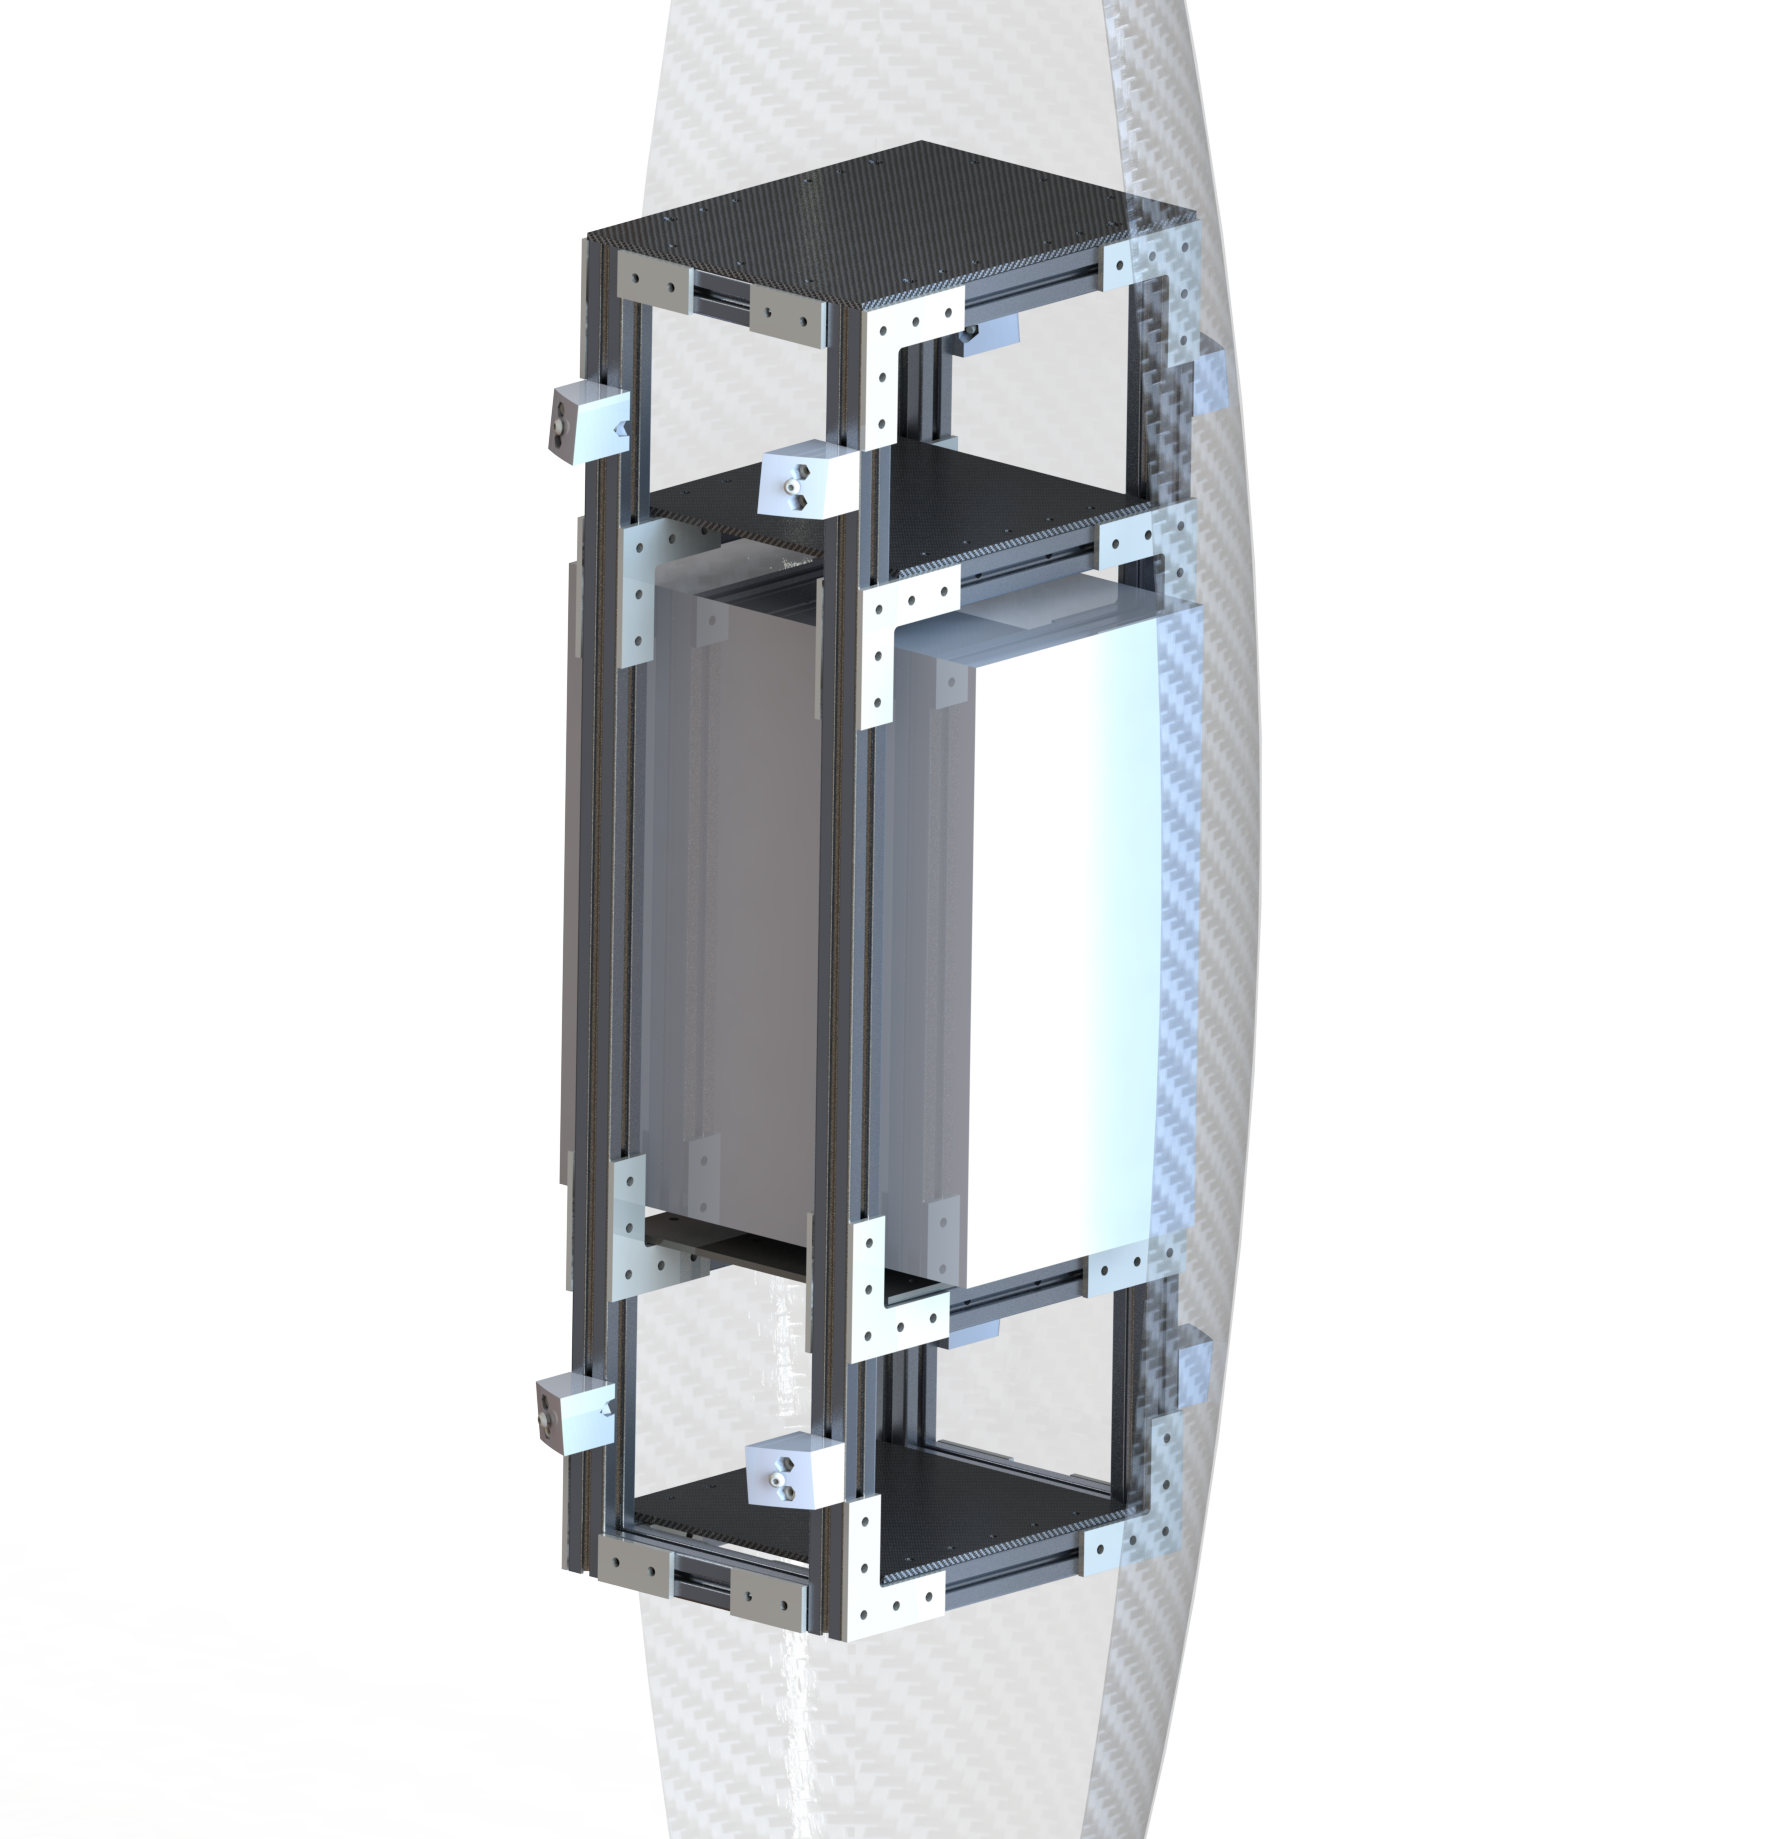
\includegraphics[width=0.8\textwidth]{Aeroshell/Aeroshell3.png}
  \caption{\label{fig:aeroshell3}Internal structure with middeck locker rendering.}
\end{figure}

\subsection{TUMBR}

\subsubsection{Tether}

\indent\indent For the tether, the final material selection is 1/4" diameter Spectra rope from Mazzella. The properties are an upgrade from the previous iterations material selection of kevlar. A factor of safety of 1.2 was added to make the total length of 670 m for a 9 second drop.

\subsubsection{Tether Guide}

\indent\indent The final design for the tether guide is the rolling ring drive. The subsystem consists of a drive motor, transmission belt, rolling shaft, and the drive itself. The rolling ring drive, shaft, and supports are mounted at the front of the platform between the roller and the reel. The drive motor is mounted at the back of the platform. The transmission between the motor and the rolling shaft consists of two pulleys and a v-belt. The motor is wired into the batteries underneath the platform. The pitch of the box is set prior to use. This will be how fast the box housing moves along the rotating shaft and is dependent on how fast the tether needs to be wrapped along the reel. When releasing the aeroshell the motor will be turned off, allowing the tether to unreel without the rolling ring drive being engaged. 

\subsubsection{Brakes}

\indent\indent The final design for the second generation system will be similar to the first generation except with hardware upgrades. The design will utilize a singular disk and rotor setup, which is normally used by trucks for towing boats,and will include hardware which is a direct upgrade compared to the Honda Fit hardware. This includes a larger brake rotor, a dual piston caliper, and high performance brake pads. The brake system was chosen because of the need to handle a large load for an intermediate amount of time. The large, veined, and vented rotor allows for massive convective forces to cool the rotor under large loads, preventing warping issues. The shaft which the brake rotor will be mounted on is designed to include a dual brake caliper setup, however for this iteration only a single set up will be used for the 2 second demonstration. The brake rotor is attached to a mount which is welded to the shaft, which makes maintenance or replacement very easy for the user [Fig. ~\ref{fig:Mount3}]. The caliper is mounted to the platform using a 7075 high grade aluminum adjustable mount which can raise and lower the caliper setup for ease of access to the brake pads and caliper pistons  [Fig. ~\ref{fig:Mount2}].The mount was custom designed to allow for ease of manufacturability via laser by having the components laser cut, instead of using an CNC. This design choice made the braking components less expensive and quicker to get, while still maintaining very good tolerances. 

\begin{figure}[H]
  \centering
  \includegraphics[width=0.9\textwidth]{TUMBR/Brake_Setup_1.png}
  \caption{\label{fig:Mount3}Brake Setup}
\end{figure}

\begin{figure}[H]
  \centering
  \includegraphics[width=0.9\textwidth]{TUMBR/Mounts.png}
  \caption{\label{fig:Mount2}Adjustable Mount - Side View}
\end{figure}

The master cylinder, which holds the brake fluid, is attached to the base plate via two L-brackets and is perfectly in-line with a linear actuator which meshes with the master cylinder. The master cylinder will produce a ratio of 1:5.22 to provide the force required by the system to slow the aeroshell, payload, and tether. The linear actuator will provide 400 lbs of force into the master cylinder and is also attached to the base plate using hardware provided via the manufacturer.The Linear actuator is integrated with and optical encoder to ensure the precise load is being applied to the braking system. The linear actuator shaft is fitted with a custom 3D printed nozzle to provide a perfect fitment between the linear actuator and master cylinder. The amount of force needed to stop the aeroshell, payload, and tether for a 9 second drop is 8,878 Newtons. With the 400 lb force of the linear actuator and a master cylinder ration of 1:5.22, the force output of the braking system is approximately 9,500 newtons of force, which is enough to halt the system.

The forces on the mounting hardware was also considered when designing the components. The bolts used have a 12.9 class shear strength which equates to around 732 MPa. When calculating the maximum force, it was found that at the maximum force of 8,898 N, the shear stress experienced per bolt would be 19.6 MPa. This gives a safety factor of 37 when considering the shear force on the bolts used. The material used for these mounts was 7075 aluminum which is rated for 500 MPa yield strength which exceeds some steels. With the rated yield strength, the 7075 aluminum mounts will have no problem handling the forces required.



% ---------------------------------------------------------

\subsection{Controls \& Instrumentation}
\input{Controls/controls_final_design_specs}

% ---------------------------------------------------------

\subsubsection{Unit and Reel}

\indent\indent Through the iterative design process encountered throughout the manufacturing process, our group solidified the design of the platform and reel system, which is presented below in [Fig. \ref{fig:TUMBRHiQual}]. 

\begin{figure}[ht]
  \centering
  \includegraphics[width=1.0\textwidth]{TUMBR/TUMBRHiQual.png}
  \caption{\label{fig:TUMBRHiQual}High-Quality render for integrated platform and reel system.}
\end{figure}

With the design of every subsystem being finalized and fit-checked through CAD, the ultimate design of the platform, or metal plate that everything mounts to, was chosen to be 40.5 x 50 inches. Using SolidWorks FEA simulations to analyze the platform deflections encountered during the braking process where the highest loads would be encountered, we selected a platform thickness of 0.25 inches. We arrived at this by using a conservative (higher than we expect) load of 6000 N applied through the base of the spool frame with theoretical U-bolts as balloon mounting points to keep the system static. Original considerations for materials revolved around the use of different types of steels. However, upon further analysis of other metals and their strength to weight ratios we instead chose 7075 aerospace grade aluminum, which has superior strength to weight properties compared to steels of similar dimensions. This allowed us to achieve the same strength characteristics while coming in at 1/3 the mass. 7075 aluminum also has the added benefit of being tested and proven in high-altitude situations. It is commonly used in the manufacturing of airplanes and other aerospace applications where the material is put through much more rigorous loading scenarios. The 7075 aluminum was sourced by Alro Metal Services in Orlando. A unique service this metal supplier provides is laser cutting. This allowed for all of the holes in the platform to be pre-cut prior to pickup, which made user-end manufacturing and assembly process much simpler. The drawback was that it cost our team time in the sense that we spent a greater deal of time finalizing the CAD design such that every hole was placed perfectly. 

The reel system was composed of five main parts: the spool frame, the high-speed, high-load bearings, the shaft, the rotor mount, and the tether housing walls. For a visual representation, the final design of the reel system is depicted below in [Fig. \ref{fig:UnitReelHiQual}]. 

\begin{figure}[ht]
  \centering
  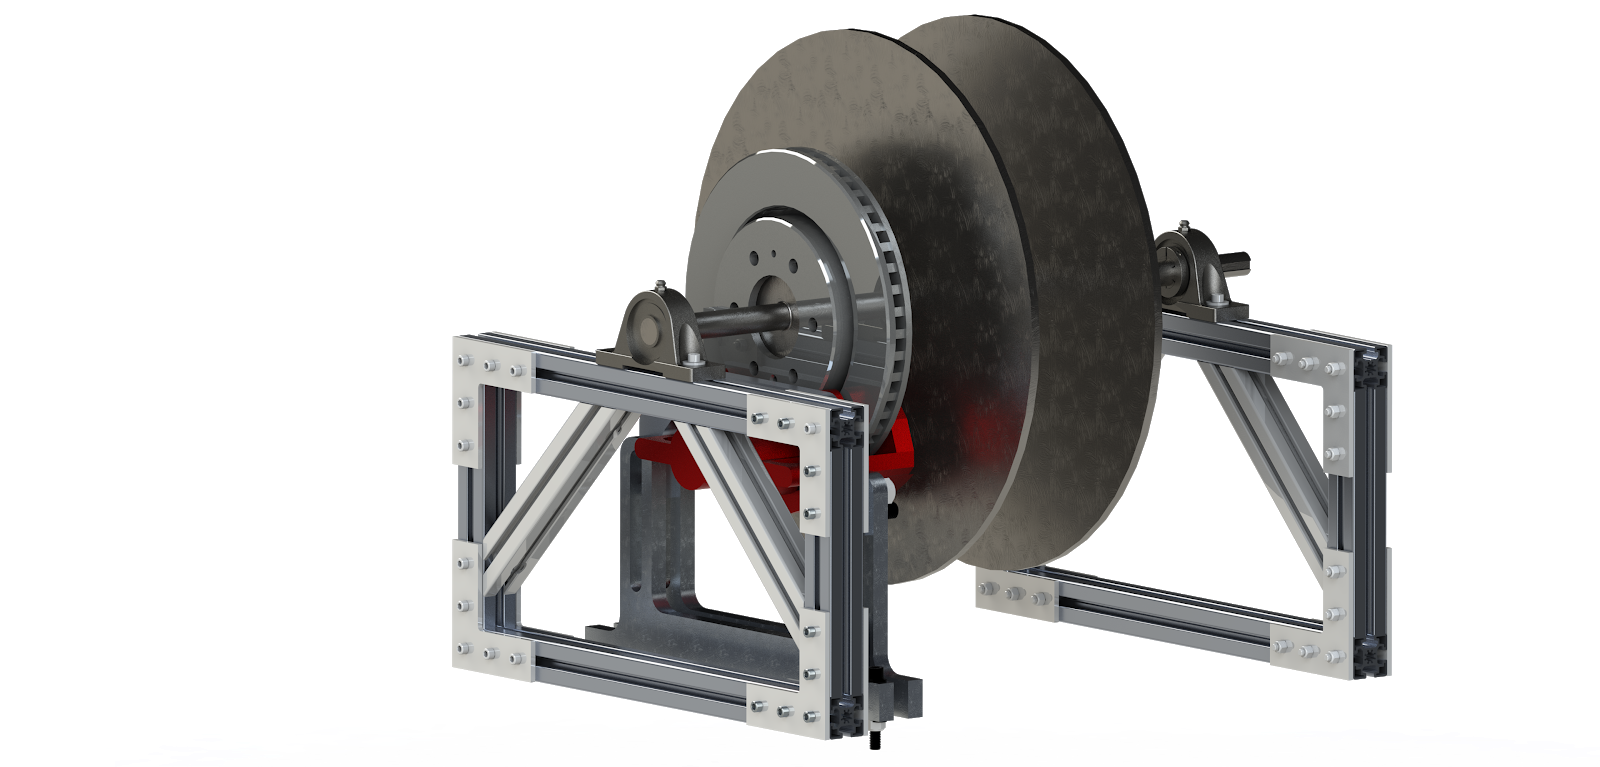
\includegraphics[width=0.9\textwidth]{TUMBR/UnitReelHiQual.png}
  \caption{\label{fig:UnitReelHiQual}A high-quality render of the reel system final design.}
\end{figure}

The design of the spool frame deviated from the original concept presented by the first-generation low-cost microgravity team. Rather than using an x-frame design made from welded steel with a central mounting point for the shaft, we chose to use 8020 aluminum with a half-x-frame design. This decreased the mass of the frame, the amount of material used, made the manufacturing process much more simplified, and greatly reduced cost, while still providing a safe, robust, and strong support for the highest-loading scenarios we would expect to encounter. Five to six double-hole corner gussets were then used to fix the base of the frames to the platform. 5/16 inch screws were used to secure these structures together.

The bearings we selected were chosen for their high-speed, high-loading, and low operating temperature characteristics. They allowed for easy mounting of the shaft and were fixed securely to the 8020 aluminum frame. 

The three remaining structures, the shaft, rotor mount, and tether housing walls, were all made from various alloys of carbon steel. Carbon steel was chosen over other types of steel for it's superior machinability and weldability. 

The previous first-generation low-cost microgravity team had a similar design but encountered several problems in the manufacturing and assembly of their shaft, rotor mount, and tether housing walls. In particular, the weld between the rotor mount and the shaft was off-center, which in other words meant that the rotor mount was not perfectly perpendicular to the central axis of the shaft. This was a catastrophic mistake that rendered the entire part useless. The off-plane rotor mount, which the brake rotor was then fixed to, created a wobble when the shaft was rotated, which prevent the rotor from aligning with the caliper, therefore disallowing the brakes to every properly engage. 

To circumvent this issue we introduced a design modification to our shaft. Rather than having the shaft itself be a single constant diameter throughout it's entire length, we instead stepped down the diameter at points where structures would be expected to mount to. To provide more detail, the shaft was thickest in the center, at 1.5 inches. At key points from the center of the shaft the diameter is decreased by only several millimeters. This design then allows for the rotor mount and tether housing walls to have a perfectly perpendicular surface to rest against during the welded process, which ensures that they too will be perfectly perpendicular to the central axis of the shaft. After machining and welding, we found this design characteristic to produce the results we desired. The final assembly, with all parts in place is shown below in [Fig. \ref{fig:RealUnitReel}]. One final characteristic to the shaft was a keyseat that was cutaway for the mounting of a freewheel bearing as detailed in the Reel Motor sections of this report. 

\begin{figure}[ht]
  \centering
  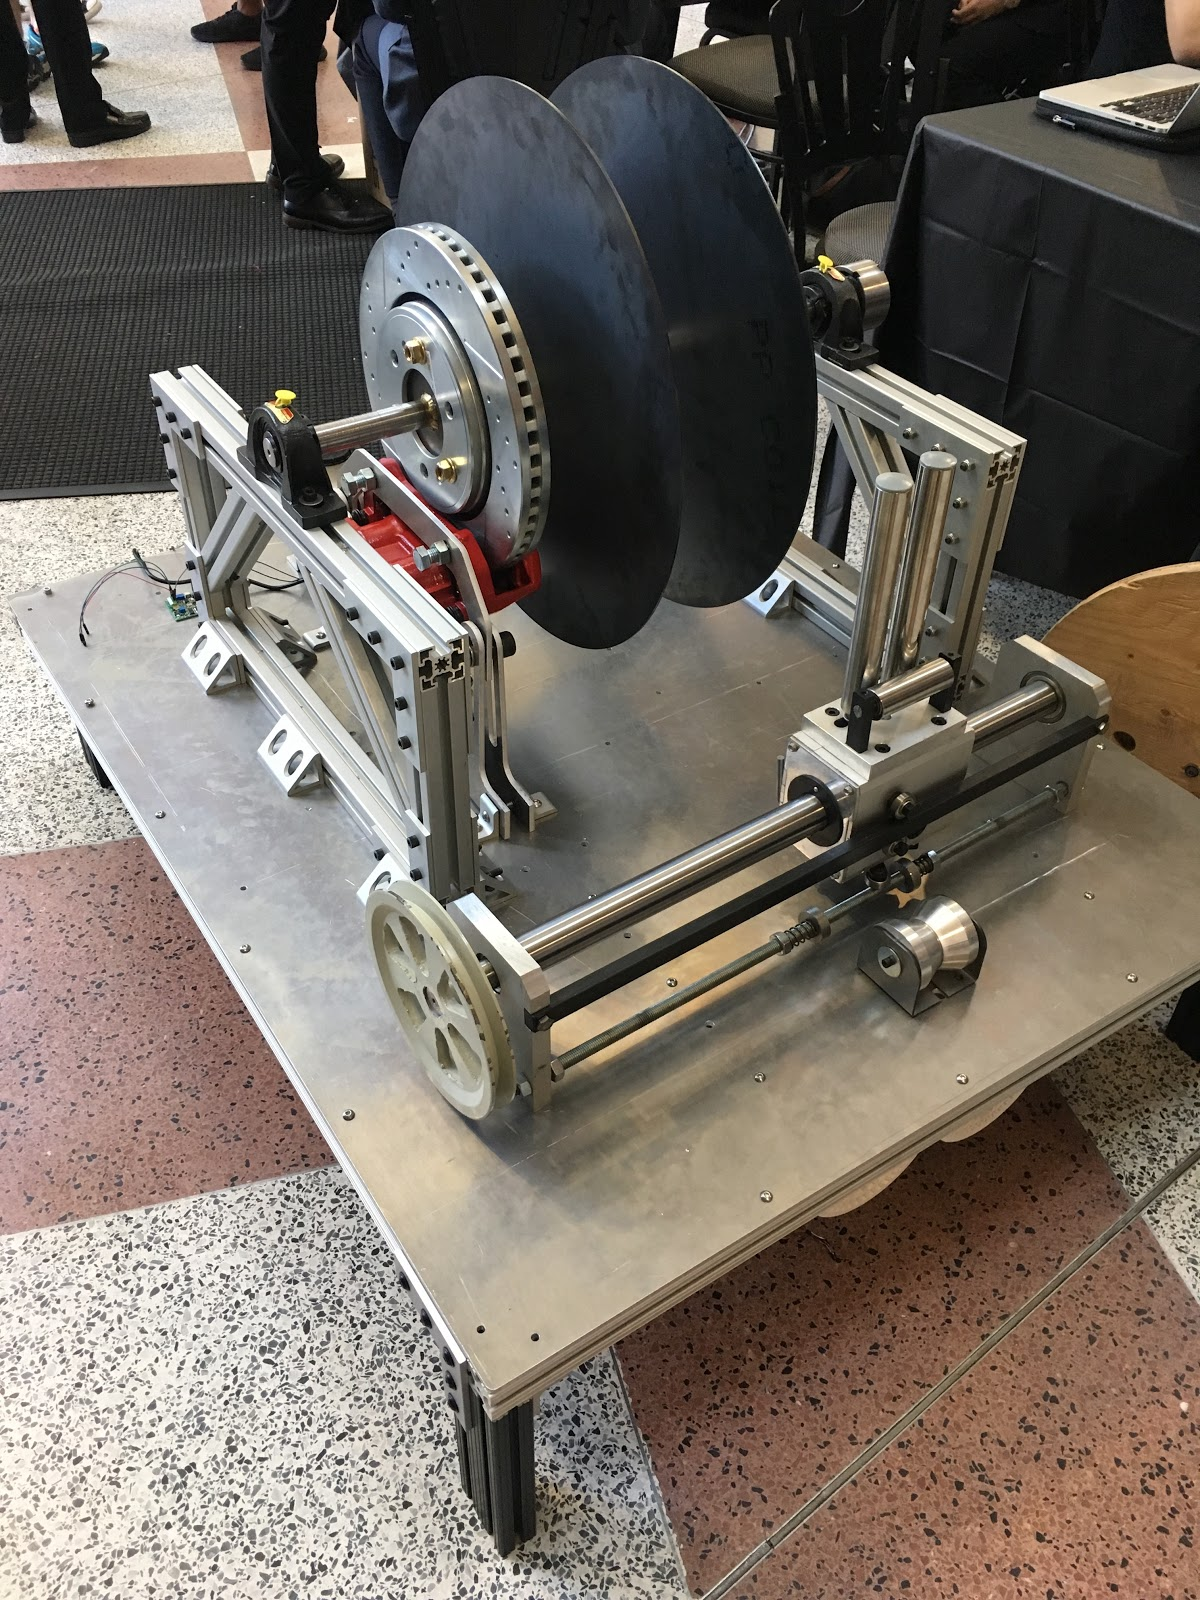
\includegraphics[width=.4\textwidth]{TUMBR/RealUnitReel.jpg}
  \caption{\label{fig:RealUnitReel}The platform and reel system as they were assembled in their finality.}
\end{figure}

The rotor mount and tether housing walls were both sourced from Alro Metal Services, where we again made use of their laser cutting services. This allowed for their simple geometries to be easily cut from a single plate for carbon fiber steel. 

All CAD drawings may be found in the Milestone 6 Final Report Data Packet found on OneDrive. 

\subsubsection{Reel Motor}

The final design of the reel motor subsystem consists of the motor, gear reducer, and transmission system. An Ampflow A28-400 BLDC motor was used in conjunction with a worm gear reducer to achieve the desired torque necessary to lift the aeroshell. The previous team used Ampflow motors with success for reeling up the aeroshell. The gear reducer was a new addition since the torque requirement is much higher in this iteration. The motor's 1/2" output shaft connects to a step up shaft adapter in order to fit into the 7/8" bore of the gear reducer. A sprocket is fitted to the output shaft of the gear reducer. Another sprocket is mounted over a freewheel bearing on the shaft. The bearing ensures power transmission only while the aeroshell is being reeled up. A size 80 heavy roller chain connects the gear reducer to the shaft.

\subsubsection{Release Motor}

The transmission system for the release motor was developed from a basic pulley system. The design incorporates an A-size V-belt, which are commonly used for medium to high speeds. The v-belt shape was chosen for its simplicity, acceptable operating conditions and low weight. Longer drop times will require higher RPMs and a more complex gear and timing belt system would be necessary, but since this system will only be applied to the 2-second drop time the materials chosen are sufficient. The release motor will drive a 2" diameter pulley directly mounted to the motor shaft. The pulley is then connected to a 6" diameter spoked cast iron pulley via a 29" long v-belt. 

The centers of the pulleys are positioned 8" apart to allow for sufficient room and expected slack in the belt. The larger pulley is mounted to a 5/8" diameter extruded key shaft to then drive the tether release disk. Both 5/8" shafts are mounted via two high-speed self-aligning ball bearings. These bearings are designed for speeds up to 7,300 rpm, which are within the requirements of a 2-second drop. 

Extensive research was conducted when selecting a brushless DC motor (BLDC) capable of meeting these performance requirements. Ultimately, the AmpFlow A28-400-F48 BLDC motor was selected. It was the only BLDC motor our group could find capable of meeting performance requirements. This motor in particular is a new flagship product of the company and because of it's novel it does not yet have any published performance spec sheets that can be used to accurately model the system. However, to remedy this lack of information our group held extensive conversations with engineers from the company to not only ensure that this motor will meet our performance expectations but to also characterize the power and electrical parameters the motor requires to meet those performance standards. From these conversations we expect to provide 48 VDC to the motor via four Apex UB12220 12V 22AH batteries wired in series. To produce the required torque throughout the duration of a drop, the motor will draw approximately 40 amps from these batteries. Interfacing between the battery, onboard computer, and electric motor is the motor controller, which will regulate the power applied to the electric motor to meet system requirements throughout the test. The motor controller we have selected is the VEX Robotics Victor BB motor controller, which is designed to accommodate up to 50 VDC and 300 A continuous, far exceeding our expectations of approximately 40 A. As mentioned in \ref{sss:PowerRisk}, it was critical to consider the proper gauge of wire for connecting all of these electrical components. It was determined that 8 gauge wire will be used in our system design, which has a maximum amperage rating of 73 amps, well above our expected load. A simple diagram of this integrated system is presented below in [Fig. ~\ref{fig:rpi_controller_motor_schem}].

\begin{figure}[ht]
  \centering
  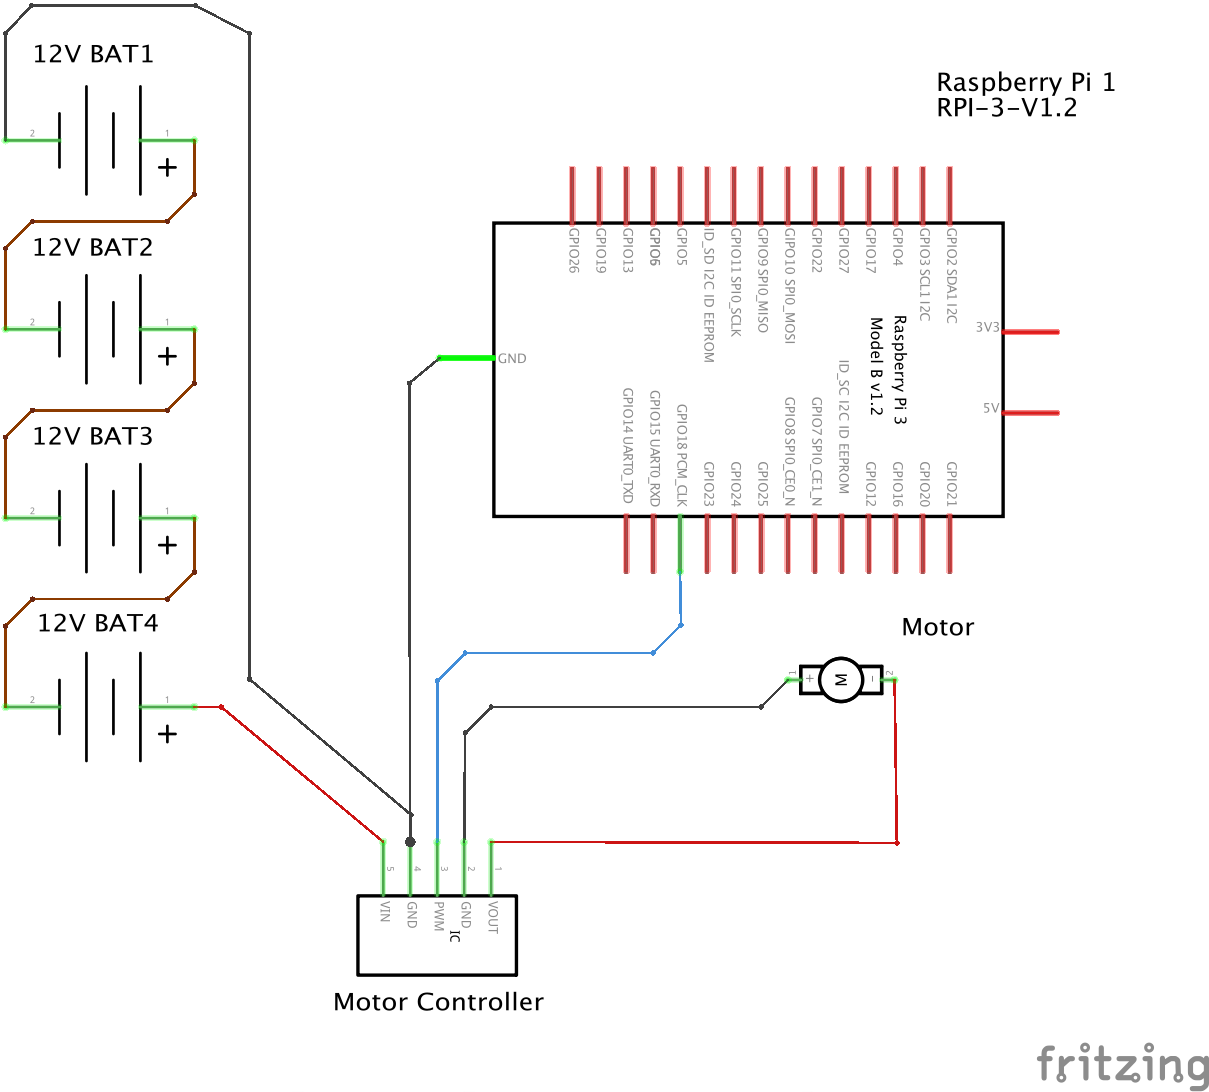
\includegraphics[width=0.8\textwidth]{Controls/rpi_controller_motor_schem.png}
  \caption{\label{fig:rpi_controller_motor_schem}Simple diagram showing the integration and connections of the batteries, Raspberry Pi, motor controller, and motor.}
\end{figure}

\indent\indent To control the electric motor the Raspberry Pi units will send PWM signals to the motor controller, which will then regulate the amount of power sent to the motor. Because there are no spec sheets on motor performance our group plans to do extensive testing to characterize this behavior and will use this data to update our model and the code used to control the motor.

\subsubsection{Power}

\indent\indent Onboard the TUMBR platform are multiple electronic systems, which include the release motor, reel motor, brake actuator, Raspberry Pi, and a later included tether guide motor. Rather than having a central battery pack with multiple voltage regulators to control the power supplied to the individual components, we decided to have multiple battery packs with only some components sharing power rather than all of them. 

The release motor requires a 48 VDC power supply capable of supplying a peak current of at least 120 amps. The reel motor as well as the tether guide motor both require a 24 VDC power supply and the Raspberry Pi requires a 5.5 VDC power supply. For the 24 VDC and 48 VDC we chose to wire two and four 12 VDC APEX lead-acid 22 AH capacity batteries in parallel to supply the required voltages. The batteries selected have a discharge rate capable of supplying the components at any given time, thus ensuring power requirements are met. For the lesser 5.5 VDC power supply we chose to connect a buck coverter across one of the aforementioned 12 VDC batteries to regulate the voltage to the required 5.5 volts. Details and spec sheets for these batteries are provided in the MS6 Final Report Data Packet. [Fig. \ref{fig:RealPower}] below shows the voltage reading across four of the 12 VDC batteries wired in series to provide power to the release motor. 

\begin{figure}[ht]
  \centering
  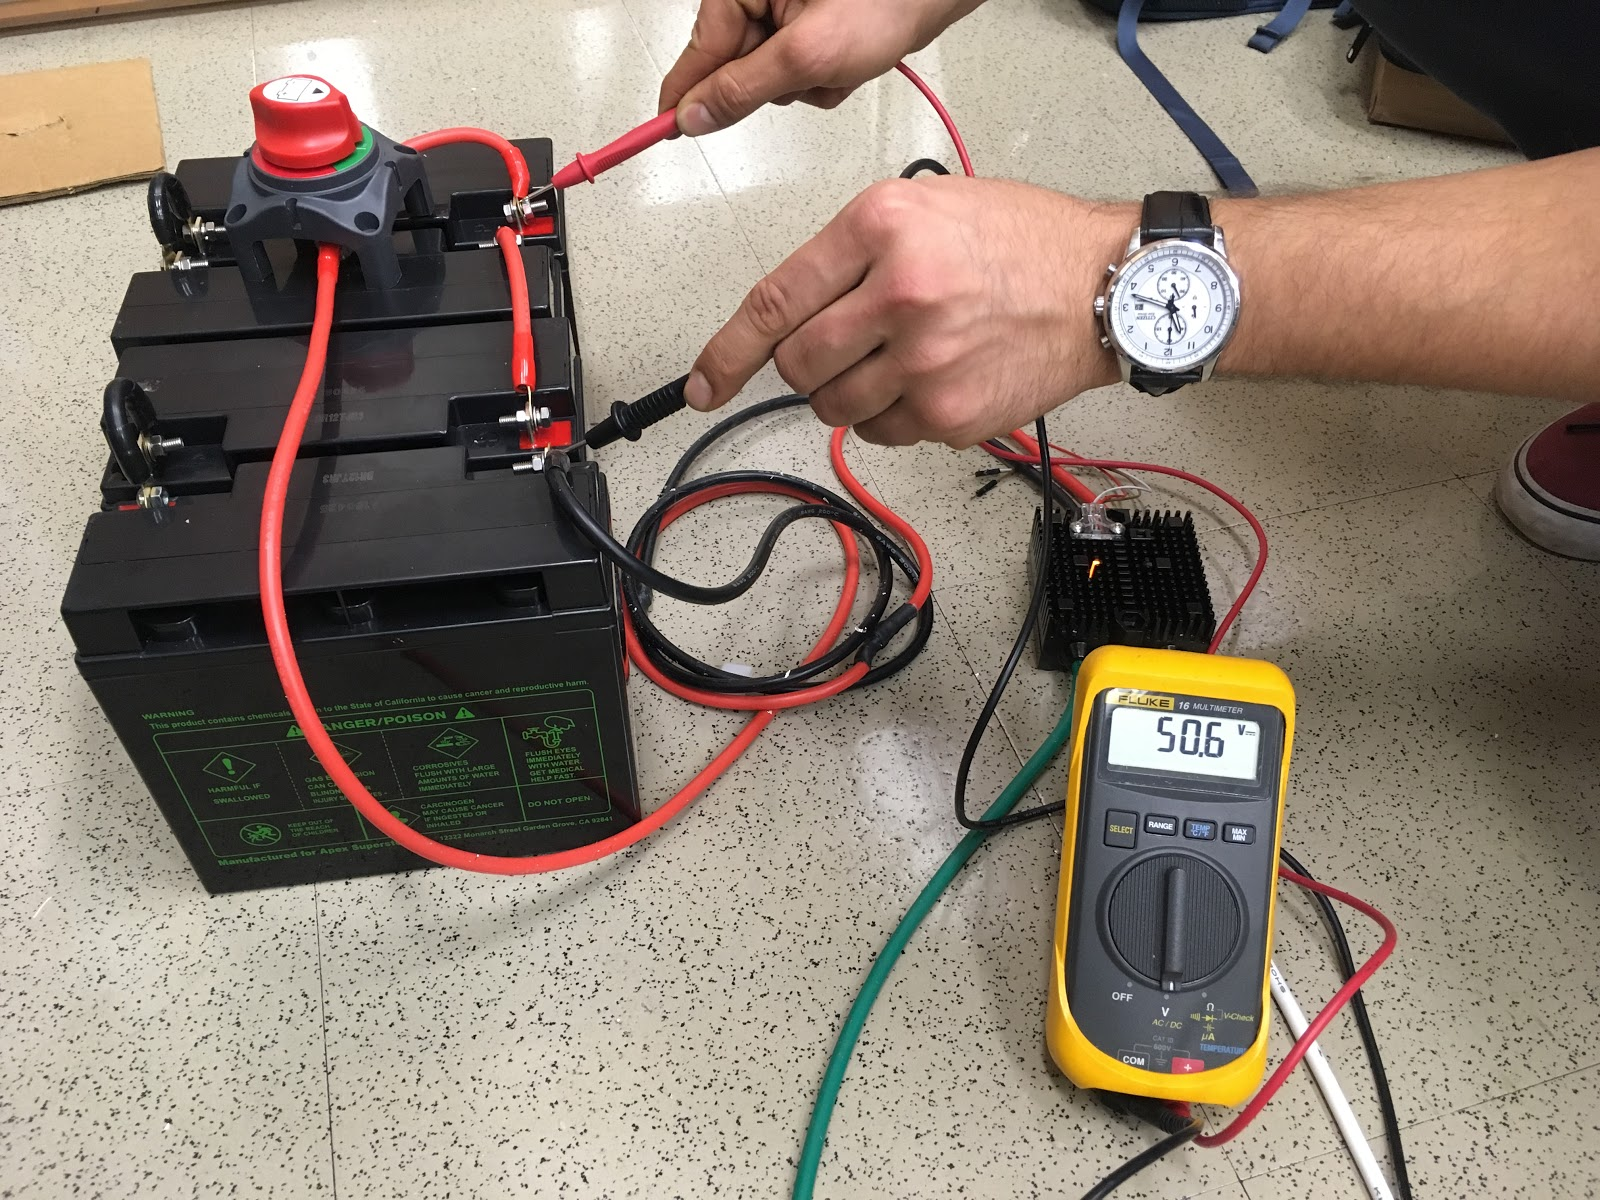
\includegraphics[width=.8\textwidth]{TUMBR/RealPower.JPG}
  \caption{\label{fig:RealPower} Four 12 VDC batteries wired in series to supply 48+ VDC to the release motors.}
\end{figure}

% ---------------------------------------------------------
% ---------------------------------------------------------
% ---------------------------------------------------------

\section{System Evaluation}

\subsection{Aeroshell}

\indent\indent The aeroshell is the part of the system that houses the payload. The payload will contain a middeck locker, which is where the actual microgravity experiment will be placed. The aeorshell will be attached to the TUMBR system via tether and will also house all the corresponding electronics. When the initial design of the aeroshell began to be developed, certain system requirements and design parameters were created to develop a realistic working model. These requirements were not only mandated by the customer, but also by the team to be able to produce a working model. The major customer requirement was for the aeroshell to be capable of achieving a state of quality microgravity for a duration of 9-25 seconds. The term “quality microgravity” means microgravity of 10-2 g’s or better. The final system must be reusable and capable of approximately six or more drops per mission. This means that the aeroshell system must be strong and rigid enough to endure the forces experienced from multiple high-speed drops, without experiencing any modes of failure such as corrosion, thermal shock, plastic deformation, and other modes of failure relating to the environment. A key requirement for the aeroshell system is that it must be reusable with minimum to zero maintenance on it during drops. Since the aeroshell will be up in the stratosphere, there will be very limited ways to fix components that break after each drop.

There have been improvements to the aeroshell from the previous iterations work. This includes a new airfoil design that makes the aeroshell shorter in length, less drag, and lighter to help the mass budget. Connecting the tether to the aeroshell subsystem has been changed due to the addition of an internal structure that will distribute majority of the braking force. The addition of the internal structure creates a housing unit for the middeck locker or payload to secure it within the aeroshell.

\indent\indent The aeroshell subsystem is comprised of two major structures. The first component is the aeroshell itself. The aeroshell structure is a modified airfoil geometry designed to be aerodynamically efficient and maintain a low drag coefficient. It will be made out of carbon fiber in order to withstand the environment, yet be light and portable. The second component is the internal structure which is found within the aeroshell. This component acts as a skeleton of the subsystem, designed to organize all the internal items including the middeck locker which will house the microgravity experiment. It is critical that these components do not fail during the mission, as they house the most important part of the project.

The risk assessment for the aeroshell subsystem is very important, because if the subsystem fails then the whole mission fails. The team has taken into account all the potential failure modes that the subsystem could encounter during its mission. The team has worked hard to ensure the success and safety of the project in designing the aeroshell subsystem. Selecting the adequate material, running accurate simulations, and refining the manufacturing method are all part of the team effort to mitigate all potential failure modes. In this section, the specific details of each failure mode will be addressed and resolutions will be proposed. 


\subsubsection{Aeroshell Structure}
\indent\indent The aeroshell structure will be manufactured using a mold that the team will create. This will ensure that the team is able to make the structure exactly as designed. The structure will be made out of carbon fiber and will be bolted together on one side. The key is to be able to open and close the aeroshell between missions. Its main purpose is to serve as a casing to the internal structure.  
\begin{table}[H]
\caption{\label{tab:aeroshell_strucure} Aeroshell Structure Failure Modes \& Probabilities}
\centering

\resizebox{\textwidth}{!}{%
\begin{tabular}{ll>{\columncolor{gray!10}}c>{\columncolor{gray!20}}c>{\columncolor{gray!30}}c>{\columncolor{gray!40}}c>{\columncolor{gray!50}}c}
\toprule
\textbf{Component} & \textbf{Mode of Failure} & \multicolumn{5}{c}{\textbf{Probability}} \\
\cmidrule{3-7}
    &   & Very unlikely & Slightly possible & Possible & Fairly possible & Highly possible \\
\midrule
Aeroshell Structure & Catastrophic Failure  &\xmark       &       &       &       &       \\
\cmidrule{3-7} %\addlinespace
                    & Unexpected Vibrations &       &\xmark &       &       &       \\

\cmidrule{3-7}
                    & Improper Assembly     &\xmark &       &       &       &       \\

\bottomrule
\end{tabular}}
\end{table}
\subsubsection*{Aeroshell Structure}
\indent\indent In the incident that the structure experiences catastrophic failure, it would put anyone involved with the experiment at risk. This means that the aeroshell would fail if the design of the structure could not withstand the forces of a high altitude drop. The failure mode is very unlikely due to the aerodynamic design of the structure. This will cause the aeroshell to drop smoothly and experience low drag. This has been verified by the accurate ANSYS CFD simulations that have been performed on the aeroshell. To mitigate this risk, the team will perform a drop test of the completed aeroshell to ensure it can travel smoothly. Another possibility of total destruction is if the material chosen is not strong enough to withstand the drop. A way to mitigate this risk is by choosing the right material for the mold. Carbon fiber was chosen as the material because of it's high resistance to destruction and deformation.

The structure could be subject to unexpected vibrations on its time traveling downward. These vibrations could be a result of crosswinds that interfere with the linear movement of the aeroshell. This could cause a failure in the aeroshell if the vibrations are too strong for the structure to handle. The possibility of this happening is slight. The team has chosen to mitigate this risk by choosing to create the aeroshell out of carbon fiber. Light, yet durable, carbon fiber is an excellent material to withstand this potential risk. In order to prove this, the team has run a vibrational analysis on ANSYS and have yielded positive results.

The last failure mode feasible for the aeroshell structure would be the improper assembly of the structure. The possibility of this happening is very unlikely. The team has spent the past few months familiarizing themselves with the best manufacturing techniques for carbon fiber molds. An error in the manufacturing is very unlikely, and if one occur ed the team would not move on with a faulty product. Once completed, the team will bolt down the open side and make sure it is sealed. A way to mitigate this failure mode is to have more than one team member inspect the structure before the mission. This is to ensure the aeroshell has been assembled properly.
% ---------------------------------------------------------

\subsubsection{Internal Structure}
\indent\indent The internal structure of the aeroshell will be made of 8020 Aluminum beams. It will have four eye-nut bolts on the top surface which will lead to a hook. The hook will be connected to the tether which leads to the TUMBR subsystem. The triumph of this connection point is critical for mission success. 
\begin{table}[H]
\caption{\label{tab:internal_structure} Internal Structure Failure Modes \& Probabilities}
\centering

\resizebox{\textwidth}{!}{%
\begin{tabular}{ll>{\columncolor{gray!10}}c>{\columncolor{gray!20}}c>{\columncolor{gray!30}}c>{\columncolor{gray!40}}c>{\columncolor{gray!50}}c}
\toprule
\textbf{Component} & \textbf{Mode of Failure} & \multicolumn{5}{c}{\textbf{Probability}} \\
\cmidrule{3-7}
    &   & Very unlikely & Slightly possible & Possible & Fairly possible & Highly possible \\
\midrule
Internal Structure  & Structural Failure     &      &       &\xmark       &       &       \\
\cmidrule{3-7} %\addlinespace
                    & Unexpected Vibrations     &\xmark       &      & &       &       \\
\cmidrule{3-7}
                    & Payload Failure           &\xmark       &       &       &       &       \\
\cmidrule{3-7}
                    & Improper Assembly         &\xmark &       &       &       &       \\

\midrule
Tether Connection   & Structural Failure        &       &       & &\xmark       &       \\
\cmidrule{3-7}
                    & Fatigue Failure         & &       & \xmark      &       &       \\

\bottomrule
\end{tabular}}
\end{table}
\subsubsection*{Internal Structure}
\indent\indent The structural failure of the internal structure would be a direct result of the loads it will experience during the braking and reeling process. The probability of this occurring over time is possible, but not fairly possible since the material chosen for the internal structure is durable. The team has chosen to mitigate this risk by performing FEA analysis on the main 8020 beams expected to handle the heavy loads. The team will also conduct tests to ensure the strength and durability of the internal structure once it is manufactured. The team will also have to routinely expect the internal structure to ensure it has not started to succumbed to any of the forces it has experienced. 

The same failure mode of unexpected vibrations that applies to the aeroshell also applies to the internal structure. The main difference is that the probability of failure decreases in the internal structure. If any unexpected vibrations where to occur, the outer structure would absorb most of the vibrations and the ones the internal structure would feel would be damped down. A way the team can mitigate, besides the vibrational analysis, is to physically test the internal structure to see how it reacts under these type of conditions.

Payload failure of the internal structure has a very unlikely risk. It would be very difficulty for a payload failure to occur since the internal structure has been designed to fit the middeck locker nice and snug. This means that it will not have room to move around and the possibility of it failing in that manner is nearly impossible. It will also be strapped in securely. A way the team could mitigate this risk would be by ensuring that the payload is secured before every trial. The other way a payload could fail would have to do with aeroshell controls which will be discussed in the next section. 

Lastly, the improper assembly of the aeroshell would cause failure. The event of this occurring is also very unlikely since the team will be mindful and careful when manufacturing this important component. The best way to mitigate this failure mode is to have several team members inspect the internal structure before the aeroshell is clasped around it. 

\subsubsection*{Tether Connection}
\indent\indent The biggest worry that the internal structure has is the tether connection. The highest possibility of failure in the entire aeroshell subsystem is found in the tether connection. Structural failure at this point is fairly possible. This is because of the heavy loads that this connection point is experiencing it. If the load is too much for the connection to handle, the aeroshell and internal structure would come flying down with no way to stop it. There are two ways to mitigate this. First, the team will run FEA simulations on ANSYS, specifically on the mounting points, to ensure that they can handle the expected loads. Secondly, the team will physically test the mounting points by attaching heavy loads to it and dropping them a certain distance. This will ensure the strength and reliance of the mounting point. 

Another important failure mode to account for is fatigue failure. This failure mode is a real possibility. After several drops, the bolts that make up the mounting point might begin to wear down or even come loose. A loose eye-bolts could create a fatigue failure and the result would be catastrophic. The best way to mitigate this risk is to have the eye-bolts checked regularly between drops, and tightened if required. If the bolt is showing signs of fatigue, a replacement must be ordered immediately. With regular inspection, the risk probability does not loom large. 

% ---------------------------------------------------------

\subsection{TUMBR}

\indent\indent The TUMBR unit was not completed and fully integrated in time for the conclusion of Senior Design 2. From the Milestone 5 documentation our group had plans for thorough and comprehensive testing to demonstrate system capabilities. Despite not having a system in it's fully integrated and functional state, we were still able to evaluate several concepts and subsystems.


One of the main concerns about the braking system was that the rotor would not be welded on perfectly on the vertical axis causing unwanted braking during certain parts of shaft rotation. This unwanted braking would have put a larger torque requirement onto the motors which would cause the system to fail. Notches were created in the shaft to prevent the rotor from being mounted off axis. This combined with a modular and adjustable mount, ensured that the braking system would not encounter this problem. The caliper and master cylinder were tested when first assembled and work as expected. When the master cylinder bore was pushed in, the brake caliper pistons would squeeze towards each other. Both the caliper and linear actuator were tested individually and proven to work, however the integration of the two was not tested. This was due to bad luck, as the SD card which had the code to control the brakes had snapped and the code was lost. However, both systems of the brakes were mounted to the platform and are ready to be tested together. 

As for the motor controller, the team was able to integrate the motor controller provided by VEX Robotics with a PID controller and an optical rotary encoder to adequately change the speed of the release motor. However, due to the lack of a testing facility, no testing was performed on the integrated system. Nonetheless, a proof-of-concept testing was done in the lab that consisted of rotating the release disks by hand to demonstrate that the code provided by the CS team for the motor control was fully functional and operational. In addition to the motor controller, testing was done on the linear actuator responsible for applying the brakes. The CS team was able to demonstrate their capability to fully extend and retract the actuator in accordance to the desired drop time. In other words, during a drop simulation, the actuator was fully extended while the system was waiting for the drop command, as soon as the drop command was sent the actuator retracted releasing the brakes, and as the desired drop time was reached the actuator was extended again.

\subsubsection{Tether}

\indent\indent The tether we selected for this project was deemed to require no testing where our group instead favored to rely on the accuracy of the manufacturers performance specifications and the fact that the loads we expect to encounter are much less than the ultimate strengths the tether is capable of of. A risk assessment was carrying out on this component though and is detailed below along with risk mitigation strategies. 

\begin{table}[H]
\caption{\label{tab:tether_failure} Tether Failure Modes \& Probabilities}
\centering

\resizebox{\textwidth}{!}{%
\begin{tabular}{ll>{\columncolor{gray!10}}c>{\columncolor{gray!20}}c>{\columncolor{gray!30}}c>{\columncolor{gray!40}}c>{\columncolor{gray!50}}c}
\toprule
\textbf{Component} & \textbf{Mode of Failure} & \multicolumn{5}{c}{\textbf{Probability}} \\
\cmidrule{3-7}
    &   & Very unlikely & Slightly possible & Possible & Fairly possible & Highly possible \\
\midrule
Tether      & Structural Failure    &       &       &\xmark       &       &       \\
\cmidrule{3-7} %\addlinespace
                & Over Elongation       &       &     &\xmark    &       &       \\
\cmidrule{3-7} %\addlinespace
                & Abrasion       &\xmark &       &       &       &       \\
\cmidrule{3-7} %\addlinespace
                & Torque       &\xmark &       &       &       &       \\
\cmidrule{3-7} %\addlinespace
                & Water Absorption       &\xmark &       &       &       &       \\
\cmidrule{3-7} %\addlinespace
                & UV Resistance       &      &       &\xmark &       &       \\

\bottomrule
\end{tabular}}
\end{table}

\indent\indent The tether adds more risk to the overall system. It provides the main connection between the aeroshell and main unit. A failure of the tether would result in the aeroshell becoming a projectile threatening the safety of anyone on the ground below it, which is a major violation of FAA regulation for people operated vehicles at these altitudes. With that said, the failure of the tether would certainly result in an FAA investigation of the situation. This would be terrible for the team and school's reputation, not to mention the safety to those below the falling aeroshell. The tether would be prone to large amount of forces with a lot of material swaying throughout stratospheric crosswinds. This could cause the tether material to elongate, stretch, and eventually brake. However, this has been taken into account with the material selection of the tether, but it would be a possible outcome due to unforeseen weather events in the stratosphere.

\indent\indent It is expected that the tether will unspool from the reel system at a maximum rate of 6,000 rpm. Due to the large amount of forces that the tether would be experiencing, the possibility of tether abrasion would be a risk toward the system. Also, the tether would be experiencing torque forces throughout the flight and could eventually create an unstable system. To mitigate this risk we recommend any operators of this system to fully understand the lower and upper level wind shear and weather the day of light to ensure reasonably stable conditions. To further diminish the risk of tether failure, proper inspection should take place after and before every mission. This includes but is not limited to looking for signs of fraying, splicing, knotting, or any other potential defect.
% --------------f-------------------------------------------

\subsubsection{Tether Guide}

\indent\indent The tether guide consists of three main components. The drive shaft, drive motor, and roller bearings are all important to the function of the tether guide. All the components must be working properly to ensure the tether is wound evenly along the reel.

The implementation of the tether guide came up short. It was realized too late into the project that a third motor to control the tether guide would be required. As such, testing was not able to be carried out on the tether guide. However, we did carry out a risk analysis assessment for the tether guide and highlighted risk mitigation strategies for the component. 

\begin{table}[H]
\caption{\label{tab:tether_guide} Tether Guide Failure Modes \& Probabilities}
\centering

\resizebox{\textwidth}{!}{%
\begin{tabular}{ll>{\columncolor{gray!10}}c>{\columncolor{gray!20}}c>{\columncolor{gray!30}}c>{\columncolor{gray!40}}c>{\columncolor{gray!50}}c}
\toprule
\textbf{Component} & \textbf{Mode of Failure} & \multicolumn{5}{c}{\textbf{Probability}} \\
\cmidrule{3-7}
    &   & Very unlikely & Slightly possible & Possible & Fairly possible & Highly possible \\
\midrule
Drive Shaft     & Catastrophic Failure      &\xmark &       &       &       &       \\

\midrule
Roller Bearings & Total Destruction         &       &       &       &       &\xmark \\
\cmidrule{3-7}
                & Overheating               &       &       &\xmark &       &       \\
\cmidrule{3-7}
                & Catastrophic Failure      &       &\xmark &       &       &       \\
\cmidrule{3-7}
                & Failure to Engage         &       &\xmark &       &       &       \\

\midrule
Drive Motor     & Overheating               &       &       &\xmark &       &       \\
\cmidrule{3-7}
                & Inoperable Temperature    &       &       &       &\xmark &       \\

\bottomrule
\end{tabular}}
\end{table}

Catastrophic failure for the drive shaft would result in complete loss of functionality for the tether guide. This failure mode is unlikely since most of the load in the tether will be distributed along a roller attached to the platform. However, it will experience some load as the guide traverses it. To mitigate this risk testing will be performed on the shaft and structure of the guide to ensure its integrity.

The roller bearings are located within the housing of the tether guide and make direct contact with the drive shaft. These bearing will eventually wear down over time and result in slipping along the drive shaft. Regular maintenance and repairs can completely mitigate this risk. There is a fair probability of the bearings overheating since they are driven through friction. This could lead to warping and a failure to engage. Inspection and maintenance can mitigate this risk. Catastrophic failure of the bearings could occur if they are put under a very heavy a load. The result would be failure to engage and loss of function of the tether guide. The tether guide was chosen with consideration to the load it would be put under which makes this mode unlikely. Further testing can prove the strength of the bearings and mitigate this risk.

One of the most likely modes of failure is the drive motor overheating. This could be due to heavy loads the motor wasn’t designed to take. An inefficient motor will also overheat due to power not being fully transmitted into torque. Overheating of the motor can lead to stalls or complete loss of functionality. Mitigation of this risk mostly comes down to selection of the motor itself. Selecting the correct motor and designing it to maximize heat transfer away from the motor will ensure overheating does not occur. 

% ---------------------------------------------------------

\subsubsection{Brakes}


\indent\indent Risk assessment of the braking subsystem can be decomposed into five main components.  The brake pads, calipers, rotors, master cylinder and actuator all have individual effects and modes of failure which can be seen in [Table ~\ref{tab:braking_system_failure}].

Our team was unable to carry out integrated testing with the brakes. While test plans were discussed early in the semester, the braking system could not be tested fully without the rest of the platform fully completed. Due to this constraint, the only testing done was with the brakes separate of the system with very low loads applied. Testing with the loads anticipated would have identified modes of possible failure which were not thought of preemptively however, the list below depicts many of the possible failure modes which can occur while under heavy load braking. 

\begin{table}[H]
\caption{\label{tab:braking_system_failure} Braking System Failure Modes \& Probabilities}
\centering

\resizebox{\textwidth}{!}{%
\begin{tabular}{ll>{\columncolor{gray!10}}c>{\columncolor{gray!20}}c>{\columncolor{gray!30}}c>{\columncolor{gray!40}}c>{\columncolor{gray!50}}c}
\toprule
\textbf{Component} & \textbf{Mode of Failure} & \multicolumn{5}{c}{\textbf{Probability}} \\
\cmidrule{3-7}
    &   & Very unlikely & Slightly possible & Possible & Fairly possible & Highly possible \\
\midrule
Brake Pads      & Total Destruction     &       &       &       &       &\xmark \\
\cmidrule{3-7}
                & Uneven Wear           &       &\xmark &       &       &       \\
\cmidrule{3-7}
                & Brake Fade            &       &       &       &\xmark &       \\
\cmidrule{3-7}
                & Improper Assembly     &\xmark &       &       &       &       \\

\midrule
Calipers        & Uneven Wear           &       &       &\xmark &       &       \\
\cmidrule{3-7}
                & Failure to Engage     &       &\xmark &       &       &       \\
\cmidrule{3-7}
                & Catastrophic Failure  &\xmark &       &       &       &       \\

\midrule
Rotor           & Uneven Wear           &       &       &\xmark &       &       \\
\cmidrule{3-7}
                & Weld Cracks           &       &\xmark &       &       &       \\
\cmidrule{3-7}
                & Warping               &       &       &       &\xmark &       \\

\midrule
Master Cylinder & Lack of Pressure      &       &\xmark &       &       &       \\

\midrule
Actuator        & Failure to Engage     &       &\xmark &       &       &       \\

\bottomrule
\end{tabular}}
\end{table}

The brake pad has a slight possibility of the brake pad itself coming loose out of the caliper which could be caused by poor assembly, unexpected forces, or poor maintenance. This risk of this failure can be mitigated through regular maintenance and checkups between flights to ensure the brake pads stay properly seated inside the calipers. The brake pads also have a fair probability of experiencing uneven wear due to poor assembly, which can be remedied by careful assembly and inspection after assembled. Due to the load experienced by the brakes, it is probable that brake fade will occur causing longer breaking time because of overheating. Overheating can be reduced by allowing the braking components to cooled fully in-between drops. There is a high probability which the brake pads will become destroyed due to overheating, high loads, and accelerated wear. Through visual inspection, all of the risks associated with brake pads can be detected. Although having many high-risk factors, brake pads are consumable items in which the risks can be mitigated by having regular inspections and maintenance. After a certain life expectancy or accelerated wear is found, the brake pads can be replaced at a relatively low cost.

The brake calipers have a slight possibility of catastrophic failure due to material fatigue and strength when large loads are being applied.  There is a fair probability that uneven wear will occur on the caliper, causing some o-rings and metal clamps to become more worn than others due to poor assembly. This risk can be mitigated by carefully constructing and mounting the caliper to the unit. Through regularly cleaning and visual inspections of the brake calipers the two previous risks can be mitigating by ensuring no cracks, rust or corrosive materials are on the caliper. There is also a fair probability that the calipers will not engage enough to put adequate pressure on the rotor to stop the aeroshell. This can be caused by failure in o-rings, brake fluid evaporation, or poor assembly. Visual inspections for brake fluid leakage or gases in the master cylinder on a regular basis will prevent a caliper pressure failure. The caliper failure modes and effects are easily detectable because regular visual inspections and cleanings will show any damage or problems. Like brake pads, calipers are a low cost replacement when damage is found through inspection. Although calipers are not supposed to be replaced frequently, if found necessary through testing the calipers can be considered a consumable item.

The rotor is subjected to a large force translated from the brake pads and calipers. This force can cause a fair probability that the weld which holds the mount connecting the rotor to the shaft will fail. Visual inspections will not suffice to detect this possible failure, instead an x-ray would be necessary to penetrate through the weld in order to detect any micro-cracks growing in the weld.  It is probable that the rotor will experience warping through the combination of a large heat flux and large translated forces from the brake pads. To mitigate this risk, post flight inspection is required to detect any warping in the rotor. This inspection will have to be with a precise tool which can detect whether the rotor is still aligned while spinning. If warping has been detected, the shaft will have to be taken off the unit to detach the rotor from the mount and attach a new rotor. The mount connecting the rotor to the shaft is a crucial and non-consumable component, that if damaged will have to be re-fabricated. Where if the rotor fails, a simple disassembling of the shaft will have to be done in order to re-mount a new rotor to the shaft. 

The master cylinder houses and transports the fluid to the calipers to apply the pressure which will slow the aeroshell. There is a fair probability that the master cylinder will not give enough pressure to engage the calipers. This loss in pressure can be caused by fluid/air leaks, a loose break line which decouples under a large pressure, material failure or poor assembly. All the risk modes associated with the failure of the master cylinder can be mitigated by post flight visual inspection and ground testing. Ground testing will ensure the calipers are clamping the rotor and no brake lines or air leaks are present, where a visual inspection will ensure no brake fluid is leaking at the connections of the lines. 

The actuator which applies the force which will be amplified by the master cylinder to apply the pressure which clamps the calipers onto the rotor. There is a fair probability that the actuator doesn't engage due to power loss, poor assembly, jamming, overheating or stalling. To mitigate these risk a pre-flight ground test will ensure that there is enough power in the system to operate the actuator and to make sure that it doesn't stall or overheat during the process. 

% ---------------------------------------------------------

\subsubsection{Unit and Reel}

\indent\indent The platform unit and reel system were successfully manufactured and assembled in time for the engineering Senior Design Showcase. Our team was able to demonstrate that the reel system, along with the platform that every subsystem is mounted to, is capable of being designed in a way that allows for easy manufacturing, assembly, and maintenance all while requiring very little end-user modifications. We were able to demonstrate that through design and careful machining the rotor mount could be attached precisely perpendicularly, which enables a fully functional braking system. 

Our group however was unable to carry out any sort of testing of the reel and platform system with applied loads. While it was discussed early in the semester that there may be a possibility for drop testing at an off site location, this unfortunately never came to fruition. Therefore, any extensive load testing of the platform and reel system was always out of the scope for this project. However, our team did carry out a risk assessment of the structures and included appropriate risk mitigation strategies, which are detailed below. A comprehensive listing of the identified modes of failure and their probabilities are displayed below in [Table ~\ref{tab:unit_reel_failure}]. 

\begin{table}[H]
\caption{\label{tab:unit_reel_failure} Unit \& Reel System Failure Modes \& Probabilities}
\centering

\resizebox{\textwidth}{!}{%
\begin{tabular}{ll>{\columncolor{gray!10}}c>{\columncolor{gray!20}}c>{\columncolor{gray!30}}c>{\columncolor{gray!40}}c>{\columncolor{gray!50}}c}
\toprule
\textbf{Component} & \textbf{Mode of Failure} & \multicolumn{5}{c}{\textbf{Probability}} \\
\cmidrule{3-7}
    &   & Very unlikely & Slightly possible & Possible & Fairly possible & Highly possible \\
\midrule
Reel/Shaft      & Structural Failure    &\xmark &       &       &       &       \\
\cmidrule{3-7} %\addlinespace
                & Bearing Failure       &       &\xmark &       &       &       \\

\midrule
Unit/Platform   & Structural Failure    &\xmark &       &       &       &       \\

\bottomrule
\end{tabular}}
\end{table}

Structural failure of the system was the most obvious risk hanging over the operation of this system. While the probability was deemed unlikely, due diligence was still practiced to ensure that this mode of failure would not be realized. The result of any sort of structural failure would as least lead to a mission and loss of data and at most resort in a total loss of vehicle. To mitigate this risk, the structural integrity of this system was or will be thoroughly analyzed via finite-element-analysis (FEA) simulations under relevant loading scenarios. Computer simulations of dynamic loading scenarios provide evermore accurate insights into the stresses and strains a system may experience. Successful simulations showing that our system will be well within endurance limits provides us with confidence that the probability of structural failure of this subsystem is truly a highly unlikely scenario and will pose very little risk to the successful operation of our system. 

To further ensure the reliability of our system throughout it's lifetime, we recommend that frequent and thorough checks of the the structure should be carried out before and after every flight, similar to how airplanes are subjected to thorough inspections at periodic intervals. It should be obvious that our system will indeed experience extreme conditions as it persists in stratospheric conditions that include increased radiation, potentially corrosive atmospheric gases, and thermal stresses. These sort of environmental conditions tend to wear a system after multiple operations. For these reasons, an inspection plan that includes a thorough qualitative inspection of all structures, welds, joints, screws, and other components is recommended to extend the systems lifetime of safe operation and decrease the likelihood of any sort of structural failure. 

The bearings of the system can be considered a sub-component of the overall unit and reel system but are a critical component nonetheless. The probability of failure has been modeled to have a fair probability. The bearings that our group have selected have been selected with the extreme conditions in mind that our system is expected to encounter. As such, the performance specification sheets given by the bearing distributor indicates that these bearings are capable of safely operated under the expected conditions. This alone gives us confidence that the likelihood of failure is quite low, however we consider a thorough testing procedure to ensure to supplement this. This includes numerous tests of the bearings under expected loading conditions. A qualitative analysis of the bearings will take place after ever test and any signs of premature wear will be noted. 

The consequence of failure of the bearings would at least result in degraded microgravity conditions and at most result in a mission abort without loss of system. An inspection protocol for the bearings before and after every flight is also recommended. It should be understood, though, that bearings, much like many other components that experience dynamic loading, have limited lifetimes. Our design permits the ability to easily replace these parts after excessive wear is indicated, thus allowing an extended lifetime of the entire system. 

% ---------------------------------------------------------

\subsubsection{Reel Motor}

\indent\indent One of the goals for the system is the capability for multiple drops and this repeatability directly relies on the reel motor. Its function is simple, but its importance is crucial. The motor must work along with the transmission to make sure the aeroshell can make it back to the balloon for consecutive drops.

\begin{table}[H]
\caption{\label{tab:reel_motor} Reel Motor Failure Modes \& Probabilities}
\centering

\resizebox{\textwidth}{!}{%
\begin{tabular}{ll>{\columncolor{gray!10}}c>{\columncolor{gray!20}}c>{\columncolor{gray!30}}c>{\columncolor{gray!40}}c>{\columncolor{gray!50}}c}
\toprule
\textbf{Component} & \textbf{Mode of Failure} & \multicolumn{5}{c}{\textbf{Probability}} \\
\cmidrule{3-7}
    &   & Very unlikely & Slightly possible & Possible & Fairly possible & Highly possible \\
\midrule
Electric Motor  & Overheating               &       &       &       &\xmark       &       \\
\cmidrule{3-7} %\addlinespace
                & Inoperable Temperatures   &       &       &\xmark &       &       \\
\cmidrule{3-7}
                & Power Failure             &       &\xmark &       &       &       \\

\midrule
Freewheel       & Bearing Failure           &       &       &       &       &\xmark \\
\cmidrule{3-7}
                & Improper Assembly         &\xmark &       &       &       &       \\
\cmidrule{3-7}
                & Catastrophic Failure      &\xmark &       &       &       &       \\

\midrule
Gear Reducer    & Overheating               &        &\xmark       &   &       &       \\
\cmidrule{3-7}
                & Improper Assembly         &\xmark       &        &       &       &       \\
\cmidrule{3-7}
                & Catastrophic Failure      &\xmark &       &       &       &       \\

\bottomrule
\end{tabular}}
\end{table}

\indent\indent  As with the previous motor, the reel motor also has a fairly probable chance of overheating. The reel motor is at risk of being overloaded which leads to stalls or complete failure. The selection of the reel motor was made based on the power output requirements for the system. Paired with the gear reducer, the motor will be able to handle the weight of the aeroshell. 

\indent\indent The freewheel ensures the reel motor will not be spun backwards during the drop period. All of the failure modes result in loss of transmission of power and inability to reel up the aeroshell. Bearings in the freewheel will wear over time and need to be replaced. Regular inspection and replacements will completely mitigate the risk of bearing failure. If the freewheel is not properly mounted to the reel shaft it could cause uneven wear and make bearing failure more likely. The design of the shaft accommodates this by having a flat indent to push up on that will ensure proper placement. If the bearings are put under a heavy load it can’t take  they will completely fail resulting in a loss of transmission of power. The selection of the freewheel and testing can mitigate this risk. 
	
\indent\indent The gear reducer converts high rpm input of the motor to a higher torque output with lower rpm. If the gear reducer fails, then the motor will not have enough power to reel up the aeroshell. There is a slight probability of the gear reducer overheating due to heavy strain or improper lubrication. The selection of the gear reducer was made with the heavy torque load in mind to mitigate this risk. Regular maintenance and inspections will ensure proper lubrication. There is a very unlikely chance of the assembly being the cause for failure. If the gear reducer isn’t properly secured to the platform then the heavy torque load will spin it right out of its mount and result in loss of power transmission. Strong mounting points will be made to ensure this doesn’t happen. Catastrophic failure has a very unlikely chance to occur if the gear reducer is put under a load it wasn’t designed for. Like the failure mode for overheating, the selection of the gear reducer was made to handle more than the torque required by the system.


% ---------------------------------------------------------

\subsubsection{Release Motor}

\indent\indent Testing on the release motor itself was never able to be carried out. We selected the component such that it would met our design specifications. Our group had extensive conversations with the engineers from AmpFlow, the manufacturer of the motor, to understand the operation of the device as well as it's limits and capabilities, to ensure that the component that we selected would be suitable for our purposes and capable of being used. However, we received the code package from our joint computer science team too late in the senior design course to properly integrate and test the motor using their code architecture. However, testing was carried out on the motor controller itself, which was detailed in the preceding sections. Therefore, our group is confident that so long as the motor functions as advertised, the control of the motor will be achieved. Validation of this of course will only come with future testing. However, our group has explored all avenues of motor failure modes and has made significant efforts to mitigate as much risk as possible. A chart displaying the failure modes, along with their probabilities is displayed below in [Table ~\ref{tab:release_motor}]. 

\begin{table}[H]
\caption{\label{tab:release_motor} Release Motor Failure Modes \& Probabilities}
\centering

\resizebox{\textwidth}{!}{%
\begin{tabular}{ll>{\columncolor{gray!10}}c>{\columncolor{gray!20}}c>{\columncolor{gray!30}}c>{\columncolor{gray!40}}c>{\columncolor{gray!50}}c}
\toprule
\textbf{Component} & \textbf{Mode of Failure} & \multicolumn{5}{c}{\textbf{Probability}} \\
\cmidrule{3-7}
    &   & Very unlikely & Slightly possible & Possible & Fairly possible & Highly possible \\
\midrule
Electric Motor  & Overheating               &       &       &       &\xmark &       \\
\cmidrule{3-7} %\addlinespace
                & Performance Failure       &\xmark &       &       &       &       \\
\cmidrule{3-7}
                & Inoperable Temperatures   &       &       &\xmark &       &       \\
\cmidrule{3-7}
                & Power Failure             &       &\xmark &       &       &       \\
\midrule
Transmission    & Belt Slip                 &       &       &\xmark &       &       \\
\cmidrule{3-7} %\addlinespace
                & Belt Elongation           &       &\xmark &       &       &       \\
\cmidrule{3-7}
                & Warping of Pulleys        &\xmark &       &       &       &       \\
\bottomrule
\end{tabular}}
\end{table}

The first, and perhaps most likely mode of failure is overheating. No motor is 100\% efficient, meaning that of all the power generated within a motor, a significant portion of that power will be converted to heat due to the these inefficiencies. The motor that our group selected has an efficiency of approximately 85\%, meaning that for every 100 kW the motor produces, approximately 15 kW of power will be converted to heat. When a motor overheats, several possibilities may be realized. The motor may, at very least, stall and become inoperable and at worst the motor will be completely destroyed. Common causes of overheating are overloading of the motor (pushing the motor to its' stall torque), poor power conditions, environmental conditions, and frequent starting and stopping. These causes also classify as failure modes and their probabilities and strategies of mitigation are also considered. 

To mitigate the risk of the motor overheating, it was key that our motor, motor controller, and batteries were properly selected to ensure adequate power will be supplied and the motor will be capable of safely providing the required torque and power. Due to the nature of our operation, the motor will have an incredibly short duty cycle of 2 - 9 s of operation and then tens of minutes of downtime. Even at 85\% efficiency, this alone will ensure that a significant quantity of thermal energy will not be able to be built up in the system. Heat will be radiated away mainly due to radiation and not convection as a consequence of the tenuous atmosphere encountered in the stratosphere. To ensure that our motor will be capable of radiating away this thermal energy, the motor will have no isolation and will be completely exposed to ensure virtually all of the surface area will be capable of radiating heat away. The particular motor our group has selected has a variety of cavities running through the interior of the system that is nominally used in conjunction with a fan to run air through the system, allowing it to stay cool. Because a fan will be useless at 30 km in altitude, we are recommending that future generations of this design incorporate a cooling system that makes use of this feature and passes either compressed air or some other type of fluid through the motor to keep it cool. Due to the complexity of this, our group has not pursued this design. Heat transfer analyses were also not carried out due to lack of time and resource. However, these actions are strongly encouraged for future groups pursuing optimized designs of the system. 

Again, our group plans on mitigating the risk of overheating and the other stated modes of failure through component selection, structural design, and mission design. That is, by selecting the proper components, allowing the motor to be exposed to increase radiative heat transfer and by keeping the duty cycle of the motor short, we do not expect to encounter motor overheating. However, we will perform extensive testing of the motor under many loading conditions and at many speeds to characterize this and will work accordingly to reduce the cause and the effect. 

% ---------------------------------------------------------

\subsubsection{Power\label{sss:PowerRisk}}

\indent\indent The power system, as one might imagine, is a critical component that enables the operation of many other crucial systems including controls, motors, sensors, and brakes. Our group evaluated the design of our power system by creating all the circuits we designed and measuring the voltages across them. For example, the release motor requires a voltage of 48 VDC to be delivered to the motor controller, which then controls the voltage that is actually applied to the motor itself. Displayed below in [Fig. \ref{fig:RealPower2}] is a simple measurement taking from a voltmeter show that with our circuitry we are able to capture the 48 VDC required to deliver power to the motor controller. 

\begin{figure}[ht]
  \centering
  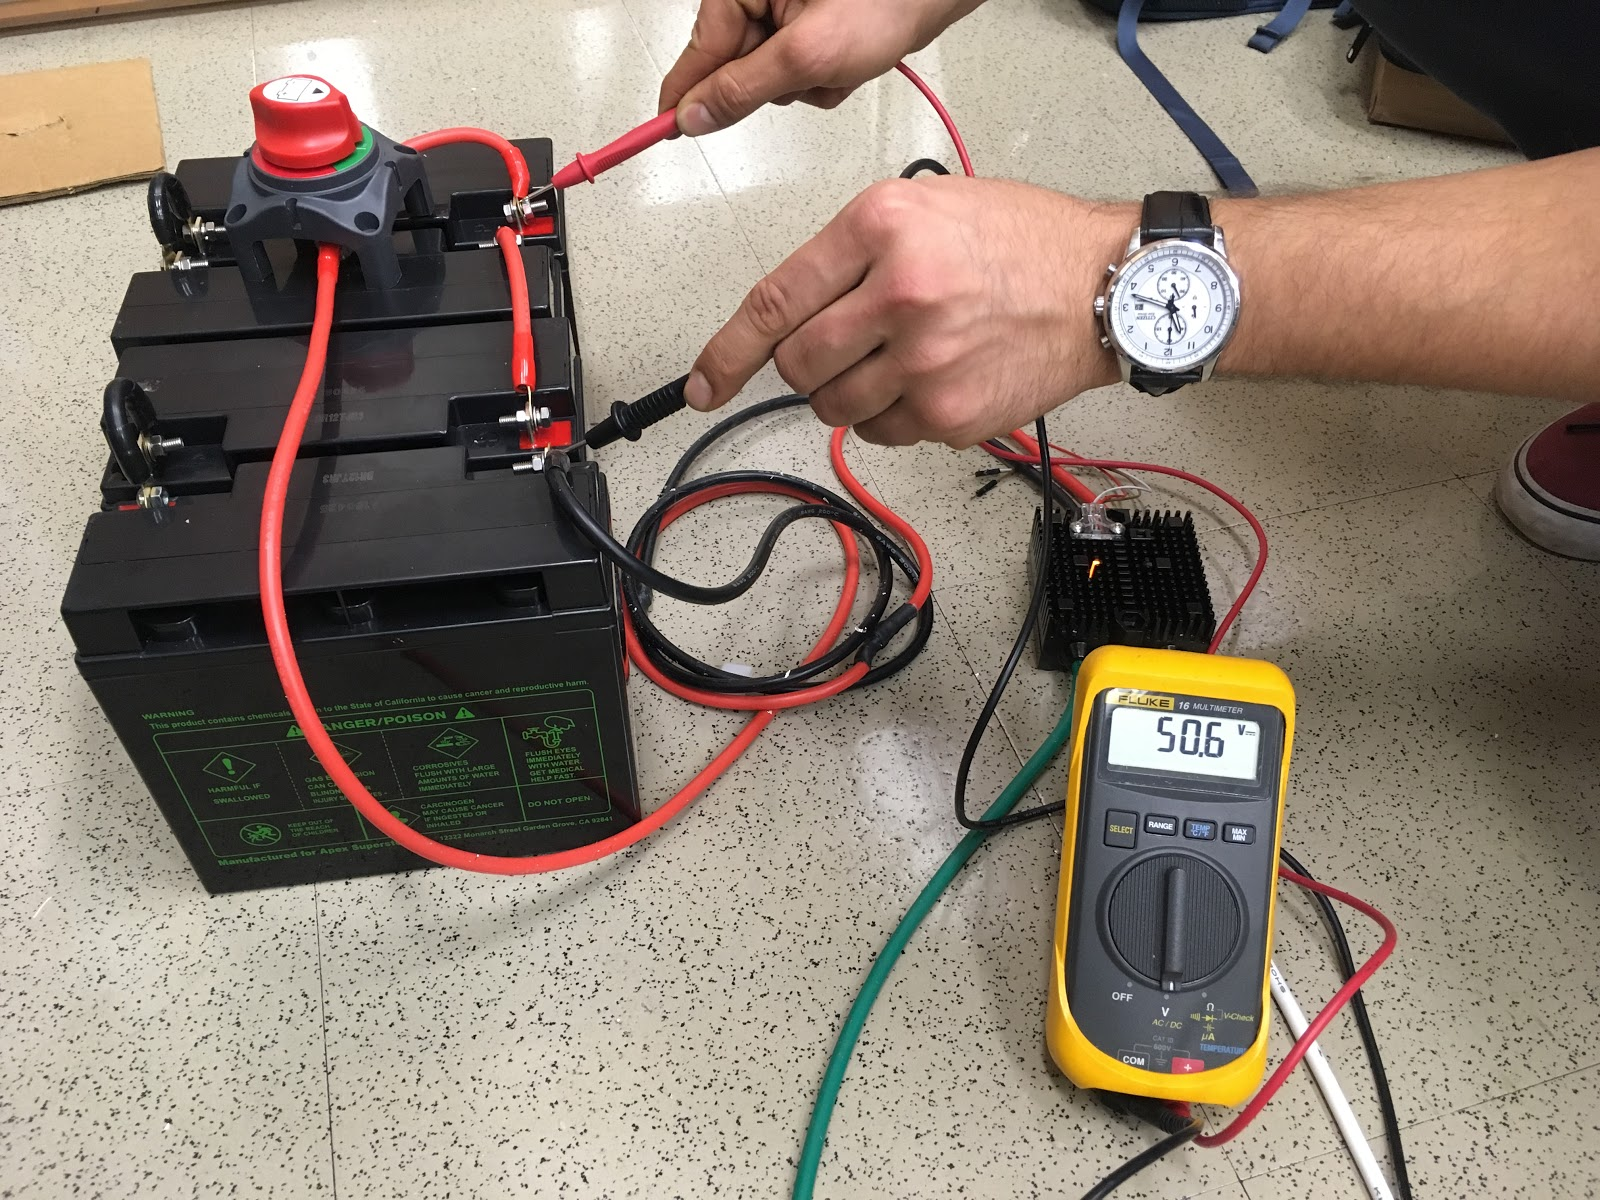
\includegraphics[width=.8\textwidth]{TUMBR/RealPower.JPG}
  \caption{\label{fig:RealPower2} 48+ VDC measured across the four APEX 12 VDC batteries wired in parallel.}
\end{figure}

In addition to the power system evaluation our group carried out, a thorough analysis of failure modes and risk mitigation strategies be explored. Three key mode failures have been identified and are documented along with their likelihoods in [Table ~\ref{tab:PowerRiskProb}].

\begin{table}[H]
\caption{\label{tab:PowerRiskProb} Power System Failure Modes \& Probabilities}
\centering

\resizebox{\textwidth}{!}{%
\begin{tabular}{ll>{\columncolor{gray!10}}c>{\columncolor{gray!20}}c>{\columncolor{gray!30}}c>{\columncolor{gray!40}}c>{\columncolor{gray!50}}c}
\toprule
\textbf{Component} & \textbf{Mode of Failure} & \multicolumn{5}{c}{\textbf{Probability}} \\
\cmidrule{3-7}
    &   & Very unlikely & Slightly possible & Possible & Fairly possible & Highly possible \\
\midrule
Release Motor Batteries & Overheating               &       &       &       &\xmark &   \\
\cmidrule{3-7}
                        & Short-circuiting          &\xmark &       &       &       &   \\
\cmidrule{3-7}
                        & Inoperable Temperatures   &       &       &\xmark &       &   \\

\bottomrule
\end{tabular}}
\end{table}

To power the electric BLDC motors our group selected lead-acid batteries for their high storage capacity, high discharge rates, availability, and relative safety and low-maintenance quality. Lead-acid batteries are widely used for a variety of industrial applications and everyday uses. When handled safely and according to manufacturer specifications they rarely pose a significant risk to the user. However, a variety of failure modes do exist. 

Overheating regularly occurs during the charging of lead-acid batteries but may only occur during operation if pushed to their peak capabilities. For this reason, we rate the probability of encountering overheating in our lead-acid batteries to be probable. If a lead-acid battery begins to overheat, the battery tends to dissipate heat relatively well through it's large surface area and connectors. It may also produce noxious gases too that, if produced in a poorly ventilated area, may pose a health risk. For this reason, during charging we plan to monitor the batteries for overheating and for any unusual smells. During operation, the battery will be well-ventilated and away from any operator or person and will pose no risk. The other key effect of overheating is a degradation in the battery itself. Overheated batteries tend to age prematurely and have much shorter lifetimes. For this reason, we plan to thoroughly read and understand all manufacturer recommendations and integrate them into our safety plan. Most importantly, our group has researched the relevant environmental conditions expected at such high altitudes and have used this information to select a battery that is expected, according to manufacturers specifications, to be capable of operating in this environment. This alone will do the most to reduce the risk of attempting to operate the battery in an inhospitable environment. 

In addition to the batteries overheating, the wires and connections also introduce a point of failure. If a user attempts to push too much current through a wire with a gauge, or diameter, that is too small the wire will overheat, which could lead to failure of the connection, arcing, and overheating of surrounding components. To mitigate the risk of this happening our group has developed a thorough understanding of the expected voltage, current, and power loads that will be placed on these wires. With that said, we are using AWG standard wire size charts to select the proper gauge of wire and corroborating these selections with battery and motor manufacturer recommendations. When properly designed, as this system will be, there will no risk of overheating in the wires. 

It was determined that the probability of the batteries short-circuiting is only a slight possibility. The result of short-circuiting may result in arcing or damage to the electronics their connected to. The only scenario in which we anticipate short-circuiting to happen is if the assembly of batteries, connectors, and wires is of poor quality. For this reason, to mitigate the risk of short-circuiting our group plans to assemble the subsystem as carefully as possible and if necessary organize and restrain wires in such a way to ensure they do not make physical connections at key points. 

\indent\indent The remaining mode of failure is the attempt to operate the battery in inoperable temperatures. For our purposes and due to the nature of the operation of the vehicle, we deemed this to be probable as a result of the expected temperatures of the upper-atmosphere we expect to encounter. The result of any attempt to operate a battery below it's minimum operated temperature would be an inability to draw the required power from the battery. This would almost likely result in a mission abort. For this reason it is incredibly important that during testing and operation in the relevant environment that the temperature of the system be monitored and a climate control system (heaters) be implemented. Our group does not expect to encounter these conditions during the testing and demonstration of our vehicle and has therefore not pursued the integration of these components into our design. Again, we strongly recommend these added components for operation in the relevant environment. 
With these failure modes accounted for and the mitigation strategies in place, our group feels confident in the safe and successful integration and operation of the power subsystem into the overall system.

% ---------------------------------------------------------

\subsection{Controls \& Instrumentation}

\input{Controls/controls_sys_eval}

% ---------------------------------------------------------
% ---------------------------------------------------------
% ---------------------------------------------------------

\section{Significant Accomplishments and Open Issues}

\subsection{Aeroshell}

\indent\indent The aeroshell has been designed better to acheive the ultimate goal of quality microgravity. It is able to be shorter to ease manufacturing, travel faster due to less drag, and weighs less than the previous iterations design. With the addition of a internal structure it has created a better way of attaching the tether to the aeroshell by not utilizing the aeroshell to bare all the braking force it will experience. By having the internal structure, it will create a better housing for the middeck locker or payload and distribute the braking throughout the whole subsystem. The team developed a way to manufacture the aeroshell in-house by using vacuum pressure.

Issues have presented themselves to be challenging throughout the manufacturing process of the aeroshell. There is an issue on the reliability and efficiency of the vacuum pressure method. The method is temperamental and leaks can be hard to find with a large object. 

There is the issue of the aeroshell reaction to environmental and braking force with the internal structure within. This is due to the processing capability of the computers provided. Simulations could not be completed due to this issue and it is a unknown.

Lastly, the issue of having a drop site for testing at sea-level conditions. This is a issue that occurred at the beginning of the project and still becomes an issue. Testing of the aeroshell needs to happen in order to show the system can function at sea-level conditions with the likely-hood of stratospheric conditions.

\subsection{TUMBR}

\indent\indent The TUMBR proved to be a much more difficult system to develop than our group initially anticipated. When scaling up the architecture to accommodate a nine second drop, the requirements for things like tether length, braking capabilities, motor power performance, etc. scales up exponentially. In particular, when a longer drop duration is being considered the amount of tether required to accommodate the drop and braking duration scales up exponentially. The more tether that is required for the drop then translates to a larger moment of inertia of the reel system as the mass and thickness (and therefore diameter) of the tether wrapped around increases. This then leads to an increased power and RPM requirement from the motor releasing the tether and the motor reeling everything back up. The increased speed of the reel system due to larger free fall velocities also creates larger braking requirements in terms of stopping torque and the RPMs the brakes can handle. 

Despite these challenges our group was able to design a system and select components to enable that virtually all subsystems would be able to accommodate the performance required for a nine-second drop duration. Detailed below are some of the key accomplishments from the individual subsystems. 

The release motor, which is responsible for ejecting the tether out at a rate equal to the free fall of the aeroshell, was required to produce torques of up to 5 Nm and angular velocities of up to 10,000 rpm. Our group was able to find only a single motor but one capable of delivering the performance required. Our group was also able to supply the transmission system and power system behind it to enable the success of the motor. However, we quickly encountered that this motor was maxing out the performance capabilities of all of the off-the-shelf (OTS) motors we were able to find. This means that in order to accommodate drop times of longer durations a custom brushless DC motor/transmission system solution would have to be worked out or future groups would have to switch to AC motors. 

The power system we designed proved to be a much simpler alternative solution to the original systems conceptualized in the first-generation of the project. Our group was able to show that we could provide the necessary power suppliers to deliver power to the various subsystems all while having enough amp-hour storage capacity for at least a several hour long mission. 

The reel system was successfully redesigned to allow for easy machining, welding, and assembly that helps ensure that the braking system in particular will be able to operate successfully. We also demonstrated that the reel system, along with the platform system, could be manufactured with relative ease and without the need for too much end-user modifications. The structure we designed is calculated to be able to accommodate the intense loading that we would expect to encounter throughout any given mission. 

The braking system was successfully mount to the unit without hindering any rotation of the shaft while disengaged. This was a large goal of the braking system since, due to poor planning and manufacturing, the previous generation's baking system was not able to rotate the shaft fully without the brake unintentionally paralyzing the rotation. The mounts created for mounting the caliper to the unit were a major success because the brake pads inside the caliper are considered to be consumable products. The mount was designed for easy repair and replacement of all the braking components, while still maintaining the structural integrate and placement of the caliper. The caliper was tested while connected to the master cylinder, and when the bore of the master cylinder was pressed in the caliper would clamp anything in between the brake pads. The optically encoded linear actuator was also tested with success, since it was able to move with great precision while applying the holding force of 400 lbs. In total, each part of the braking system successfully function as intended. However, the need to test all the functions together must still be tested.

Another key feature that our group delivered was the ability to produce a system that required very little maintenance. Unfortunately, this won't be fully proven until the system is rigorously tested and fully evaluated. However, many of the materials we've selected were designed to have long lifetimes and require very little individual maintenance. Corrosion resistant paints were purchased for the steel components to prevent possible rusting in the UV-intense radiation environment. The release wheels, which are expected to receive a significant amount of wear, are 3D printed with a high infill percentage (for strength) and are therefore easily replaced. The aluminum components were all theoretically calculated to experience very little deformations and therefore experience little fatigue over the system's lifetime. The release motors have short duty cycles, which prevents wear on the motor and overheating. The model of the lead-acid batteries were selected to requirement no maintenance whatsoever of the course of their lifetime. The tether was selected to have a high resistance to abrasion and radiation, thus extending its operation lifetime. 

Some parts, such as the brake pads and release wheels are designed to wear with time and eventually be replaced. Further instructions detailing the maintenance of these components is communicated later in the Appendix of the report in Other Manuals and Documentation. 

With all previous accomplishments considered, the entire design and product our group is producing has an estimated mass of about 300 kg, which is 100 kg less than ultimate mass budget of 400 kg outlined in our initial design requirements. While it may be difficult to source OTS components to build systems that are further scaled-up to accommodate longer drop times, there is plenty of mass budget left to allow for larger and more robust parts and components. 

% ---------------------------------------------------------

\subsection{Controls \& Instrumentation}

\input{Controls/controls_accomplishments}

% ---------------------------------------------------------

% ---------------------------------------------------------
% ---------------------------------------------------------
% ---------------------------------------------------------

\section{Conclusions and Recommendations}

\indent\indent Throughout the course of Senior Design the TUMBR team was able to deliver on some of our key goals and accomplishments. The previous first-generation senior design teams were tasked with determining the feasibility for system that would be able to enable affordable microgravity conditions by dropping a payload from the stratosphere. Ultimately, these teams produced a conceptual model showing that, to some extent, the system may be capable of production. The primary goal of our senior design team was to scale up their architecture to produce a system that is capable of delivering a nine-second drop duration that enables high-quality microgravity conditions. Here, we present the conclusions of our engineering efforts and our recommendations moving forward.

\subsection{Aeroshell}

\indent\indent The aeroshell is a critical system of the project. The team based the design of the aeroshell from the previous iteration by choosing a teardrop shape. The aeroshell subteam decided that the airfoil used previously could be improved, so 2D analysis on XFoil was done with 20+ different airfoils. This narrowed the airfoils down to three, which were selected to generate into CAD models. The airfoils were ran through a MATLAB code to optimize them. This was necessary to further decrease the drag coefficient, as well as to produce a more efficient airfoil. 4,500 iterations later, and the team finally found a final airfoil to use. The Eppler 3838 Hydrofoil was chosen. In order to accurately compare this airfoil with the previous teams airfoil, the previous airfoil was scaled up by 1.15 to fit a middeck locker vertically. After analyzing the $C_p$ distribution graphs, the $C_p$ vector distribution, and the weighted ratings evaluation, the Eppler E838 Hydrofoil was chosen to be the main airfoil for CFD testing. The purpose of CFD was to determine the drag force, pressure distribution, and drag coefficient. The CFD testing served to further strengthen the choice of airfoil, since the results yielded showed improvement of the previous iteration. Vibrational analysis and thermal analysis were also performed on the aeroshell. The vibrational analysis showed that little vibration would occur, thus the payload would not be severely disrupted during flight. The thermal analysis showed that the aeroshell would receive a temperature increase towards the middle and trailing edge. This is important to note and take into consideration when placing the components of the aeroshell. 

\indent\indent The internal structure was a concept not considered in the previous iteration. It’s main purpose is to create a shelving within the aeroshell, where the payload and electronics can be placed. This creates a designated area for the inner mechanisms of the aeroshell and provides ease when placing the components. The material selected for the main structure was 80/20. The internal structure also was designed to include the tether mount. The tether mount is pivotal to the project since it is what connects the two systems. The design created is simple, yet effective. It is composed of four eye nuts connected to the top of the internal structure with 5/16” bolts passing through two parallel 80/20 beams. This serves to disperse the load across 4 points. Heavy lifting hooks capable of locking in and swiveling will be attached to these eye nuts at one end, and attached to the tether at the other end. A simple force distribution was calculated on the internal structure to assure its effectiveness. It was calculated, after deceleration had occurred, for the tether to experience 770 pounds of force. The force that the beams could hold exceeded the 770 pounds, thus the team decided to move on with the design.

\subsection*{Aeroshell Recommendations}

\indent\indent It is recommended that further integrated simulations between the internal structure alone and the internal structure and aeroshell together. Further simulations that involved system-level testing could not be completed due to the school computer processing capabilities with ANSYS Research version and the student edition on the team's personal computers. With these simulations it would give a better idea for the reaction of the internal structure and aeroshell during the braking process. Further testing would include static structural and vibration analysis for the internal structure and explicit dynamics for the internal structure and aeroshell together.

Another recommendation is adding some type of thermal insulation to the aeroshell. As noted in the thermal analysis, the temperature peaks towards the trailing edge. Finding some low weight thermal insulation to integrate inside the aeroshell would solve this problem. It is worth exploring next semester during the manufacturing stage of the aeroshell. Another recommendation is to explore the idea of a railing system for the internal structure. The railing system would serve to facilitate the payload with reaching a microgravity state. The one major issue with the railing system is developing a braking system or padding system to avoid an major impact from happening from the deceleration. A large enough impact could destabilize the aeroshell on its way down and create a point of failure. Another issue with the railing system is the size of it is larger than the designed aeroshell.

A last recommendation is for the manufacturing process, which is a challenge in itself. With the current process that the aeroshell is manufactured, the BONDO sanding and buffing process can be improved to be more efficient, so that defects can be avoided. With the slat layout, the 69 horizontal slats can be made even wider to give a better working space when laying down the layers of carbon fiber. Taping an outline of the cutting pattern on each carbon fiber layer would be beneficial even though it is time consuming. In the long run, it is better to avoid fraying of the carbon fiber and fibers floating around the working area.

\subsection{TUMBR}

\indent\indent Our group was able to design a TUMBR system almost fully capable of accommodating a nine-second drop time while using up only 50\% of our mass budget (not considering the aeroshell structure). Furthermore, we were able to demonstrate the feasibility that a system of this nature could be produced in a way that allows for easy manufacturing, assembly, and maintenance. Save for the lack of full-scale and integrated testing, our group strongly believes that this system concept as well as the system we have been working to deliver, will be able to fulfill goals we set out to accomplish. Therefore, the big picture takeaway is that it is absolutely feasible to construct a system capable of enabling high-quality microgravity conditions for relatively long durations while being able to survive the intense environmental conditions found at high-altitudes. This system will also be capable of semi-autonomous control, as demonstrate by our joint computer science senior design team. 

While we feel that we've been able to demonstrate through design and fabrication that a nine-second drop duration is absolutely feasible, our group encountered many challenges that we feel limits the ability to scale the system up to a 25-second drop duration. The speeds, forces, and masses required to accommodate such a system well exceed the motor, braking, and material capabilities of virtually every subsystem in our system. Furthermore, imagining there was no mass budget limiting what a future team would be able to design, the scope of such a design would be well beyond what we believe an undergraduate engineering senior design team would be able to produce. The types of motors, actuators, and other systems would be more similar to those found in high-performance aerospace vehicles rather than the small-scale devices usually created within these sort of courses. 

Realistically speaking, when operating within a mass budget of 400 kg, we believe that the system would be able to accommodate for drop durations of up to only a few more seconds, perhaps 11 to 12 seconds. This however would require the implementation of electromagnetic braking, AC motors, and larger power storage and supply systems. Structurally, the materials we have produced should still be able to accommodate these longer drop durations. The true limit is simply the performance of the electrical systems. 

\subsection*{TUMBR Recommendations}

\indent\indent There are several key takeaways we would like to suggest for future teams that will be working on this project. The first is less technical but rather relates to project management. A key mistake our group made was that we became the victims of our own perfectionism. We sacrificed low-fidelity but incredibly useful experimentation using lower-quality but easily accessible materials in favor of a seemingly endless pursuit of the perfect design. As an example, the platform on the TUMBR unit our team produced is a beautiful and remarkable material we are very proud of. Because we were sourcing expensive, high-quality metal with the mounting holes laser cut into the surface, it was critical that we get the final placement of every subsystem correct so that we could predict where those mounting holes would be. The design and placement of many of these subsystems though was iterative, meaning that when one minor change was added, it would have a cascading effect on the placement of several other subsystems. This mean that the final CAD was not produced until only weeks before the engineering Senior Design Showcase. Even with a lead time of less than two weeks for the supplier to deliver the platform to us, this allowed us almost no time for subsystem integration and any kind of integrative testing. As future teams will encounter, most engineering occurs in that testing phase where problems arise, fixes are found, and a workable system is converged upon. 

The proper alternative to this would've been to purchase a lower-quality material that would not be incorporated into the final product but would have sufficed for testing purposes. A possible alternative would have been a simple sheet of plywood mounted on 2x4's that would have allowed us to simply attach the reel system with the tether and the transmission system where we could have carried out extensive testing on the tether ejection aspect of the system. All the while we could have continued to work on the actual final system and have tested the design concept to ensure that it would actually work. We missed out on these key opportunities and sold our educational experience short in favor of the pursuit for perfection. It was an oversight on our part but a learning moment nonetheless. We hope to pass this bit of wisdom on to future teams that work on this project or similar ones to prevent making the same mistake. 

Technically speaking, the braking system our team developed was intentionally meant to not accommodate for anything more than a two-second drop. This was communicated early on in the project and thus, the advanced braking system was born. Knowledge has been transferred to this team but to summarize, our team found that frictional brakes were totally unfeasible for the dynamics of the system and forces we expected to encounter. In particular, the shaft that the rotor would be mounted to is expected to spin at a maximum of approximately 6,000 rpm. The highest quality ceramic brakes used on formula-one race cars are only able to accommodate speeds of up to 2,500 rpm. Therefore, a more technologically advanced braking system- such as electromagnetic braking or air braking- needed to be developed. The development for this subsystem is constrained by the geometry, dynamics, and forces of our system but otherwise allows for open-sky designing. 

% ---------------------------------------------------------

\subsection{Controls \& Instrumentation}

\input{Controls/controls_recommendations}

% ---------------------------------------------------------

% ---------------------------------------------------------
% ---------------------------------------------------------
% ---------------------------------------------------------
% ---------------------------------------------------------


% ---------------------------------------------------------
% ---------------------------------------------------------
% ---------------------------------------------------------
% ---------------------------------------------------------



% ---------------------------------------------------------
% ---------------------------------------------------------
% ---------------------------------------------------------

\appendix

\section{\label{customer_reqs}Customer Requirements}

\indent\indent For our system to achieve mission success a payload must achieve repeatable quality microgravity conditions for a specified duration of time, while surviving extreme stratospheric environmental conditions. User needs and requirements were derived from conversations with the end custom, Dr. Adrienne Dove, and subsequent analysis implied from the users specifications. Below is an itemized list of the project goals and requirements our group determined was necessary to achieve mission success for our system. 

\subsection{Quality Microgravity Conditions}

\indent\indent The experiment must achieve 9 – 25 seconds (at least 2 seconds) of microgravity ($10^{\minus 2}$ g’s or better).

% ---------------------------------------------------------

\subsection{Environmental Considerations}

\indent\indent Both systems must be able to survive stratospheric (lower atmospheric) conditions (minimum -46\degree C and 1.12 KPa or 1\% pressure at sea level) and multiple temperature gradients as the systems ascend.

% ---------------------------------------------------------

\subsection{Reusability and Repeatability}

\indent\indent The system must be reusable and capable of approximately six or more (minimum two) drops per mission.

% ---------------------------------------------------------

\subsection{Mass Budget}

\indent\indent The entire system must operate with a mass budget of 400 Kg, therefore everything must be as light as possible.

% ---------------------------------------------------------

\subsection{Maintenance}

\indent\indent The system must be reliable and not require any maintenance between drops so that full repeatability can be achieved. 

% ---------------------------------------------------------

\subsection{Technology-Readiness-Level (TRL)}

\indent\indent Achieve a TRL of 4 as set by NASA guidelines.

% ---------------------------------------------------------

\subsection{Cost}

\indent\indent The design must be cost effective and capable of being manufactured and delivered within the Senior Design budget cap. 

% ---------------------------------------------------------

\subsection{Safety}

\indent\indent The system must have redundancies and safety factors where possible. Furthermore, the system must not pose a safety or health risk to the users, manufacturers, and general public. 

% ---------------------------------------------------------

\subsection{Portability}

\indent\indent The entire system must be portable and capable of being transported to and from testing and launch sites.

% ---------------------------------------------------------

\subsection{Strength and Durabilty}

\indent\indent Both systems (Aeroshell and TUMBR) must be strong and tough enough to endure the forces experienced from multiple high-speed drops without experiencing any detrimental plastic deformation or other potential modes of failure. 

% ---------------------------------------------------------

\subsection{State and FAA Flight Requirements}

\indent\indent The system must meet all FAA flight payload regulations for high-altitude flight. 

% ---------------------------------------------------------

\subsection{Payload}

\indent\indent The system must be able to easily and safely accommodate a middeck locker sized payload.

% ---------------------------------------------------------
% ---------------------------------------------------------
% ---------------------------------------------------------

\section{System Evaluation Plan}

\indent\indent For many systems, a prototype is needed to further comprehend the performance and efficiency. With today's technology just about anything can be designed, modeled, tested and evaluated within a computer, but there are many things that go unnoticed until they can be seen up close and in person. The objective of prototyping this system is to visually test and show the performance capabilities that were designed to, backing up the computer analysis done. A full scale prototype of our modified system will be developed to confirm the manufacturability of the system, as well as highlight efforts/talents from the team. A partial prototype was sufficient in the previous generation since it was able to meet the initial requirement milestones, but the second generation must display the capability of the system in real time. The full scale testing will take place in subsystems, while the entire system will only be tested on a previously defined partial scale. The reasoning for reducing the testing requirements on the system as a whole is a lack of space and facilities to perform the tests needed. Instead, subsystems will be able to maximize their performance in isolated tests and provide valuable results that can be complied in comparison with the partial test of the full prototype. 

% ---------------------------------------------------------

\subsection{Aeroshell}

\indent\indent The aeroshell assembly embodies the heart of the entire project as it assumes the role of courier to the sensitive contracted micro-gravity experiments. With this in mind, extensive research and testing is required in the design of the individual subsystems, namely, the aeroshell faring, the internal structure, and the controls of the system as a whole. The simulated assembly will be dynamically tested in an on-campus wind tunnel, as a 1:16.38 scale model, at ever increasing speeds as well as dropped from a substantial height to establish overall aerodynamic stability and proper weight distribution. Lastly, the internal controls of the aeroshell will be validated on the values of bandwidth, throughput, and data rate as well as the IMU, environmental sensors, and RF transmitter. 



% ---------------------------------------------------------

\subsubsection{\label{sss:aeroshell_controls_validation}Aeroshell Controls}

\indent\indent As is previously mentioned in ~\ref{sss:aeroshell_controls}, the aeroshell's controls system consists of a RPi model 3B, various sensors, and a Radio Frequency (RF) antenna, all of which are very well documented and with a huge community support. Therefore, no further prototyping is required. In spite of that, a validation process must be put in place to ensure that the controls systems is operating at the expected efficiency and project requirements.

First, the RPi will be tested for its ability to interface with all the peripherals attached to it as well as its bandwidth, throughput, and data rate. To further elaborate, one must define the difference between the terms %~\cite{%https://www.avalan.com/blog/bandwidth.-data-rate.-throughput.-whats-the-difference}.

\begin{enumerate}
    \item Bandwidth : a measurement of the ability of an electronic communications device or system to send and receive information.
    \item Throughput: the amount of data that enters and goes through a system.
    \item Data Rate : speed at which data is transferred between two devices, measured in mega bits per second (Mbps or mbps).
\end{enumerate}

To validate that the RPi has enough bandwidth to interface the all the peripherals, the RPi is going to connected to all the anticipated sensors and then some more until it reaches saturation. If the RPi's bandwidth doesn't get saturated after an extra 10 peripherals are attached to it, then it is safe to assume that the RPi is capable of communicating with all the peripherals at once.
To validate that the RPi is capable of handling the required throughput, the RPi is again going to be connected to all the anticipated sensors and then some more until it's throughput reaches a point of saturation.
Lastly, the data rate is of vital of importance as it is one of the links that govern the controls system's response rate (assuming the sensors are not the bottleneck). The data rate can be profiled by performing multiple writes and reads with one of the sensors, preferably all, to determine if the response time is adequate.

Moving on to the IMU, temperature, humidity, and pressure sensors, the sensors will be validated for accuracy and precision by collecting data in a known environmental conditions and comparing the collected data to the actual values. For instance, to validate the IMU used to measure acceleration, the IMU will be placed on a static table and data acquisition will begin. It is anticipated that the acceleration in the $x-$ and $y-$ directions is zero and the acceleration in the $z-$ direction is $-1$ since $1g$ of acceleration is applied towards the center of the earth, or downwards. Refer to [Fig. ~\ref{fig:coordinate_system}] for the co-ordinate system definition.

\begin{figure}[H]
  \centering
  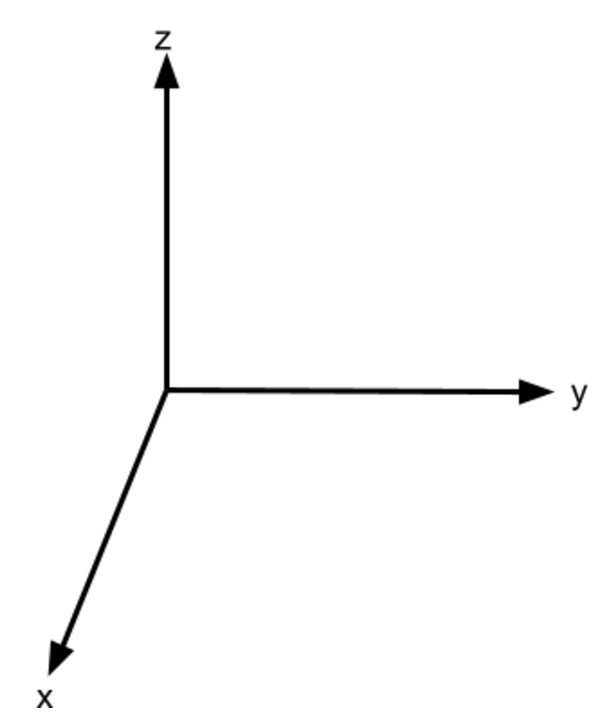
\includegraphics[width=.3\textwidth]{Controls/coordinate_system.png}
  \caption{\label{fig:coordinate_system} Co-ordinate System.}
\end{figure}

To that effect, the team is capable of validating and verifying the fidelity at which the IMU is operating. Furthermore, if random fluctuations in the readings are detected, the data can be smoothed using an exponential moving average coupled with capacitors to clean up the voltage line.

The same validation procedure could be applied to the remaining set of sensors. The non-intrusive temperature sensor could be placed in a clear line-of-sight with boiling water given that the boiling water is known to have a temperature of $100\degree C$, if the temperature readings deviate by a great deal from the anticipated value of $100\degree C$ then the sensor has failed the validation process. The same procedure is again repeated but this time while pointing the temperature sensor at frozen water knowing that the data read must be equal to $0\degree C$, again if the readings deviate from that value then the sensor has failed the validation process.

Lastly, the RF transmitter can be tested and validated by having the sending and receiving ends away from each other at a minimum distance of $30km$, approximately $18mi$. A predetermined and known string of data is then transmitted. If the received data is not the same as the sent data, or if the receiving end fails to establish communication, then the RF transmitters have failed the validation process.

% ----------------------------------------------------------

\subsection{TUMBR}

\indent\indent The components making up the TUMBR system will be tested past their expected performance ability independently and within subsystems. The tether will be tested for stretch and strength when braking force is applied, the tether guide will verify it can withstand the weight of the aeroshell, the controls will be tested for response time, brakes tested for premature wear and efficiency, the unit/reel tested for capability to withstand the torque generated from rotation, and the motors tested for operating efficiency and power consumed. By testing and verifying each subsystem independently, the tests can be catered toward a specific type of mechanism and allow a better understanding of its ability. Once these tests have been completed, the entire unit will be assembled and tested on a limited scale, further verifying all components work together as expected.

% ---------------------------------------------------------

\subsubsection{Tether}

\indent\indent Prototyping the tether consists of no alteration to the size, but to the length of the tether to sea-level conditions. The length of the tether would be cut down to accommodate sea-level testing. This would only be the case with the approval from officials at a qualified testing site with proper supervision and approved test plan procedure.

\indent\indent The full-scale of the tether provides challenges when trying to test the product to ensure that it will perform properly during flight. Testing of the tether would consist of smaller sections with multiple testing coupons. Testing would consist of elongation/torque, abrasion, water resistance, and climate (i.e. temperature) testing. Each coupon would undergo each test to receive the full effect and worst case scenario. If the coupon testing pass the worst case scenario then no further testing would be required unless otherwise noted by the FAA and their requirements.

% ---------------------------------------------------------

\subsubsection{Tether Guide}

\indent\indent A rolling ring drive was selected as the tether guide. These drives are often used in industry for similar winding applications. This subsystem has already been proven to be feasible and what remains is testing it for the project’s specific application. The tether guide also comes from the manufacturer mostly assembled except for the motor attachment.

\indent\indent Tests for the tether guide should confirm it can handle the weight of the aeroshell. To do this the guide will be mounted on a stable surface with a cable running through it. The cable will be fixed at one end with a known mass attached to the other. Spinning the shaft will drive the guide along it. Observations will be noted during testing for any signs of slippage. In order to confirm the guide is moving at the correct speed the motor will be attached to it and the pitch changed to a predetermined value. The speed and length of traversal should be proved to be accurate given a set input. For final assembly the input of the drive motor will correspond to the speed the reel is rotating at to ensure the tether is wound evenly


% ---------------------------------------------------------

\subsubsection{TUMBR Controls}

\indent\indent  As is previously mentioned in ~\ref{sss:tumbr_controls} and ~\ref{sss:aeroshell_controls_validation}, the aeroshell and TUMBR's control systems are identical except for minor additions in the TUMBR's control system that consist of a motor and brake controllers.

Both systems are sold by reputable and well established vendors. Nonetheless, both systems need to be validated to make the treatment comprehensive and for sake of completeness. The motor controller could be validated by gradually pulsing the controller using the RPi's dedicated PWM GPIO pin and noting the response time. If the controller fails to adjust the motor's speed in an acceptable time span that is to be determined during the testing phase then the controller has failed the validation process. The same procedure is again applied for the brakes controller.

% ---------------------------------------------------------

\subsubsection{Brakes}

\indent\indent The previous senior design team made the first generation prototype of this system and were unsuccessful in proving the braking system would suffice under the intense loads required. This was mainly due to poor manufacturing and assembly, not necessarily a failure in the braking system. Since we are purchasing automotive hardware with decades worth of validation, in which caliper brake system will bring a heavy chunk of moving metal to a halt, it is fair to assume that this system is completely feasible. This allows the group to skip the prototyping stage of the brake system and move straight towards manufacturing and assembling of the subsystem.

Once the brake subsystem is fully assembled, the TUMBR group will carry out a series of tests to verify and validate the braking subsystem will perform as required. The first test will to be checking the alignment and fitment of all the components and mounts to ensure the whole system is to specification with the CAD, and no unnecessary or unforeseen interference will happen. A pulley system will be rigged to translate the vertical motion of tether into a horizontal movement of tether. This will allow us to pull the tether (using a car or something similar) with a similar force to what the actual system would be experiencing, and then apply the braking to validate the brakes will bring the system to a halt. Low speed and low force tests will be preformed first, with a steady increase in speed and force until the system has achieved that similar to a 9 second drop. Once verified the braking system can perform the necessary requirements, further testing can commence to see the limits at which this braking system can achieve. This further testing can help further generations of this design to know the limits of what a brake caliper system can do for the system. 

% ---------------------------------------------------------

\subsubsection{Unit and Reel}

\indent\indent The design of the unit and reel system is largely based off of existing architecture from the first generation design. The design of the reel was optimized for the welding of the tether-housing walls, brake rotors, bearing mounts, and the reel motor adapter. The bearings and reel mount were optimized to reduce the mass and manufacturing complexity.
Despite these minor design changes our group feels confident that the operation and demonstration of the previous generation design proves the feasibility of this subsystem and allows us to go straight to the manufacturing of the improved reel system. 

Upon completion of the manufacturing our reel system, our group will carry out a series of tests to validate the integrity of the structure. A fit check of the system will first be carried out to verify the expected spacing of components from our CAD design to ensure the proper operation of the system. This includes the integration of the shaft (with welded tether-housing walls, rotor mounts, and reel motor mounts), bearings, and reel mount. The tether will then be loaded into the reel. Simply testing of the system will commence by a user simply un-spooling the tether by hand at increasing speeds. With the simple operation of the reel system verified, proper testing will begin after the release, reel, and braking systems have been integrated into the system. This will include a series of small-scale and sustained low-speed tests. Upon verification we will begin low-scale ramp-up testing, which involves the rapid acceleration via release motor and rapid deceleration via the braking system. Nominal operation speeds will be approached, met, and then surpassed by approximately 10\%. This will conclude the testing of the unit and reel and allow us to move to nominal operation. 

% ---------------------------------------------------------

\subsubsection{Reel Motor}

\indent\indent During the previous iteration of the project the team proved the feasibility of the reel motor. The current requirements for the reel motor are more stringent, but the same concept applies. In order to achieve the higher torque required a worm drive gear reducer will be in place between the motor and the reel. A freewheel one-way bearing is going to be attached to the shaft to ensure transmission of power only during the reel up phase. These components all are all part of this subsystem and all need to be tested for the load they will be under.

\indent\indent In order to test the reel motor it will need to be attached to the transmission system and integrated onto the platform. No load conditions will be tested first to make sure the motor controller is functioning properly. After verifying that the motor is getting the appropriate amount of power, loaded conditions will be applied. Weights of increasing mass will be attached to the tether in order to test how much weight the motor can take. This will include the speed the motor can wind the reel. Testing will end when the weight applied matches the aeroshell. 

% ---------------------------------------------------------

\subsubsection{Release Motor\label{sss: ReleaseMotorTesting}}

\indent\indent The preceding senior design team that owned the first generation design of this system tested their motors with marginal success. Basic operation was demonstrated, although a full-scale integrated test was never carried out. Alas, the team was able to validate the basic operational capacity of the release motor. Due to these previous tests and the relatively low-cost of the release motor system, it was decided to move straight to the purchasing and manufacturing of the full-scale components. 

Testing will first begin by simply wiring the circuit which consists of the release motor, motor controller, battery pack, and Raspberry Pi computer. With the system properly connected we will begin testing of the release motor and associated system by attempting to operate the motor via pulse-width-modulation (PWM) signals outputted from the Raspberry Pi, to the motor controller, which will pulse power from the battery pack to the motor. Our group will calibrate the motor and motor controller by exposing the system to the full-range of PWM signals, therefore setting the inputs that will go on to generate a minimum speed and a maximum speed from the motor. Basic operation of the motor under no-load conditions will then take place to ensure that the proper control of the motor can be achieved.

Following this, the belt and pulley, and release disk system will all be integrated together and into the TUMBR unit to ensure a proper fit as expected from our CAD diagrams. The tether will then be fed through the release disks. Under these loaded conditions, we will then begin low-scale and sustained low-speed testing of the motor. After verifying that the motor can sustain these low-speed loads, the tether encoder will be integrated to the system, thus providing closed-loop feedback to the Raspberry Pi and motor controller. Small-scale and sustained low-speed testing will again commence to demonstrate the precision control of the motor with the feedback incorporated into the controls. This will lead to ramp-up testing simulating nominal operating conditions and tether acceleration profiles. Short operational cycles on the order of 0.5 s - 1 s will first take place and eventually lead to 2 s - 3 s duration tests. Upon validation that proper tether accelerations have been achieved under nominal conditions, release motor testing will conclude and allow us to move on to practicing nominal operations in preparation for a system demonstration. 

% ---------------------------------------------------------

\subsubsection{Power}

\indent\indent The assembly of multiple battery packs is well-practiced by industry experts and hobbyist alike with applications ranging from automotives to amateur robotics. Because this process is so well understood and easily practiced, our group feels confident that we can move straight to the procurement and assembly of the various full-scale power systems. 

Testing of the various systems will be conducted by first validating the expected voltages across the power and ground terminals for the various battery packs. After ensuring proper voltages are produced the battery packs will then be connected to their associated systems (reel motor, release, motor, Raspberry Pi, etc.). The proper performance of the batteries with take place simultaneously with the testing of their associated systems. For example, the portion of the release motor test that demonstrates a no-load, sustained-low velocity operation will simultaneously be a test of the batteries capability to meet the performance requirements of that operation. The capabilities of the batteries will be demonstrated and validated alongside the testing of these systems and upon completion will allow us to move to nominal operations of the system. 


% ---------------------------------------------------------
% ---------------------------------------------------------
% ---------------------------------------------------------

\section{User Manual}

\indent\indent In it's fully integrated configuration the ZAP-2 system is designed to be a flight-ready vehicle capable of providing long duration and high-quality microgravity conditions for researchers and scientists to perform experimentation in. Operation of the system is a straight forward process that will be covered in two parts. Due to the interdisciplinary nature of this project, the control and logistics expertise is split across two teams. As such, the operation manual detailed below will be abridged in some aspects. For this reason we encourage readers to read through the companion report produced from our joint computer science senior design team, which details more of the ground station controls for flight operations. 

\subsection*{Pre-Flight}

\indent\indent Prior to flight, the system should be thoroughly evaluated and prepped for the mission ahead. This begins first and foremost with the charging of all battery packs and power systems. Included in the ZAP-2 infrastructural assets is a battery charging system capable of recharging all 6+ APEX 12 VDC lead-acid battery packs. The batteries should be charged to manufacturers specifications and then validated by measuring the voltage across the battery packs using any voltmeter capable of reading at least 48 VDC. 

With the batteries fully charged the user should then inspect the mechanical structures of the system. This begins by taking the appropriate size allen keys and tightening all hex screws to verify that they are in place and properly torqued. These mounting points include all gussets on the 8020 internal structure, 8020 platform support, the 8020 spool frame, the L-brackets for the spool frame assembly, the L-brackets for the caliper mount assembly, as well as the motor mounts. Using the appropriate size of wrench, the user should then properly torque all bolts on the system including those on the calipers, rotor, the caliper mount, and tether guide. All bolts or screws missing should be replaced and properly torqued. 

Following this the user should then visually inspect all structural support elements for signs of fatigue, wear, or structural compromises. The user should be looking for any cracking, deformation, corrosion, or wear. If a structure is deemed to be structurally compromised the component should be replaced prior to flight. Light corrosion can be cleaned with an abrasive or appropriate cleaner and then covered with an anti-corrosion coating such as a paint or enamel. All welds on the reel system should also be checked too for signs of cracking or wear. If the shaft system is structurally compromised it should be repaired by a welder prior to flight. Other key components to visually inspect for wear or failure include the aeroshell, all bearings, shafts, the tether, and release disks. Any material showing signs of failure should either be adequately repaired or replaced.

The release disks in particular may encounter a greater rate of wear than other metal components. This is a feature of the design. The release wheels can be replaced easily by 3D printing a new set with PLA or ABS plastic with an infill of at least 85\%. A rubber spray to increase the friction of the edge of the wheels should also be applied to increase traction of the tether to prevent slippage. 

All electrical connections should then be inspected and if necessary the continuity of the circuitry should also be checked. Any solders or wires that appear to be compromised should be replace or re-soldered. 

The braking system should also be inspected to make sure that there are no leaks and that the brake fluid is at an appropriate level. 

A simple systems check should then take place by turning on the system and then running through a yet-to-be-developed testing procedure that demonstrates that all motor and actuators that control the braking system and motors are working and capable of being controlled. We recommend a program to be developed that runs the release motor at a variety of speeds verifiable with the rotary encoder and without the tether being fed. The reel motor and tether guide motor should be run similarly. The braking actuator should show that it is capable of compression and release. 

\subsection*{Staging}

\indent\indent At the point of staging the experiment should be loaded into the internal structure and properly secured. The tether should then be fed through the TUMBR release system and fixed to the aeroshell tether mounting structure. The aeroshell then should encapsulate the internal structure and be bolted securely to it's mounting blocks. 

With the experiment intergrated and the aeroshell assembled, the reel motor should then reel the aeroshell to it's home position prior to flight. The TUMBR unit should then be attached to the launch providers balloon where it will be securely fixed to yet-to-be added mounting points. 

With all mechanical structures fully attached and set for flight the user should then power up all electronic and computer systems. For a detailed analysis for the operation and setup of the computer, radios, and ground control stationing, please read the companion report produced by the computer science senior design team. All electronics should be powered on via their switches. With communications established and all sensors reading nominally, the structure is then ready for flight. 

\subsection*{Ascent}

\indent\indent During ascent the caliper brake will be compressed about the rotor keeping the shaft thoroughly in place and preventing it from rotating. This is the "home" position of the system. All sensors should be reading values throughout the ascent process to measure the temperature, pressure, and humidity profile as a function of altitude. 

\subsection*{At altitude (30 km)}

\indent\indent Once at altitude (30 km) the system should still be in its home position. With all sensors reading values showing that the vehicle is within operational parameter, the user should prepare for the drop process. Operational temperatures should be approximately -40ºC or greater. Pressure should also be measured too to contextualize the air-resistance and drag the aeroshell is expected to encounter. 

\subsection*{Drop}

\indent\indent If the sensors show a healthy system, the user should input their desired drop time and begin the drop process by clicking the "drop" button the ground station computer. 

The drop process begins by the linear actuator releasing the calipers and thus freeing the shaft to freely rotate. Simultaneously the release motor should be activated and execute the associated drop profile depending on the user-inputed drop duration. The release motor will eject the tether at precisely or slightly faster than the free fall velocity of aeroshell to ensure that there is no tension in the tether and therefore no external forces acting on the aeroshell. The rotary encoder will measure the angular velocity of the release wheels and therefore the linear displace of the tether (assuming a no-slip condition). The rotary encoder values will then be used to provide closed-loop feedback to continuously adjust the speed of the motor to match it's desired angular velocity profile as closely as possible. All the while the accelerometer on board the aeroshell will be measuring the acceleration of the vehicle to contextualize the quality of microgravity the aeroshell was in during the drop. Temperature sensors will meanwhile be measuring the temperatures of key components such as the motors to ensure that there is no overheating. 

At the end of the drop duration the release motor will power off and the linear actuator will engage the brakes to decelerate the aeroshell at a desired rate of 3 g's. The rotary encoder will continuously measure the displacement of the tether to ensure that the aeroshell has come to a complete stop. At this point the braking system will fully compress to hold the aeroshell in a fixed position. 

With all sensors reading healthy temperature values for the electronic components the reel motor will begin to reel the aeroshell back up. The brake will simultaneously disengage to allow the reel motor to freely reel the aeroshell back in. The rotary encoder will again be measuring tether displacement throughout this process. The reel motor will only reel in the same amount of tether that was release as measured by the rotary encoder. While this is taking place the tether guide motor will also engage to precisely control the tether guide to ensure that the tether is cleanly wrapped around the spool as it is reeled back up. 

As soon as the same amount of tether that was released is reeled back up, the brakes will engage, the reel motor and tether guide motor will turn off, and the system will again be back at its home state waiting for further command. 

Throughout the entire drop process the user will have the ability to abort a drop by simply clicking the "abort" button on the ground station computer. This will premature begin the deceleration process and reeling process. The temperature of key components will be measured throughout the drop to ensure that no motors are overheating. If this occurs an abort procedure will be automatically triggered.

\subsection*{Repeat}

\indent\indent The ZAP-2 system is capable of repeated drops within a given flight. At the end of every drop the user will have the opportunity to evaluate the health of the system via on board sensors and repeat the drop process by entering a new drop time and clicking "drop". Our system does not have the ability to measure the charge of the batteries on board the flight systems but this is something that we recommend future users integrate. This will allow users to make safer decisions for how many drops they are able to execute, with the limiting factor of a flight being the charge capacity of the batteries. Until then, theoretical calculations will have to be carried out to determine how many drops the system will be capable of. 

\subsection*{Descent and Recovery}

\indent\indent Throughout the descent process the system will be remain locked in the home position. When the balloon is close to the ground the aeroshell and TUMBR system should be captured in a yet-to-be-determined process. With both structures back on the ground the TUMBR should be detached from the balloon and all electronic switches turned off to power off the system. With the vehicle safe it should be disassembled in the reverse order it was assembled. This will complete the flight operations of the ZAP-2 system.

% ---ludes------------------This inc------------------------------------
% ---------------------------------------------------------
% ---------------------------------------------------------

\section{Cost Analysis and Manufacturability Analysis}

\indent\indent This iteration of the ZAP-2 system was an exercise in the feasibility of manufacturing such a system. Many of the components and processes we've selected were meant to optimize the manufacturing and assembly process of a future system, thus delivering this novel technology as a cost effective solution for research hoping to get access to microgravity conditions for research. 

The aeroshell was perhaps the most expensive single structure to build. However, there was significant overhead that went into simply creating the mold that the aeroshell would be formed from. With this key infrastructure in place, we assume that future users will not have to provide that same overhead to create the molds for producing that part. All told, a new aeroshell should be able to be manufactured for less than \$2,000. 

The TUMBR unit need not be reproduced simply because the unit our team developed and assembled is suitable for flight. However, if one were to recreate the system we estimate it would cost approximately \%12,000 or less to do so. The most expensive items include the 7075 aluminum mounting plate (\$1,000+), the motors and motor controllers (\$1,000 for each pair), the tether (\%2,000), and the braking system (\$1,000+). The forces and performance this system is required to deliver justifies the use of high-quality and high-endurance materials, which may end up costing more than lower-quality alternatives. 

The entire expense report is listed in the succeeding section where the reader may corroborate these pricing estimates with the actual cost per item that went into producing our teams systems. 

% ---------------------------------------------------------
% ---------------------------------------------------------
% ---------------------------------------------------------

%\section{Expense Report}
\include{Expenses/aeroshell_expense_report}
\include{Expenses/platform_expense_report}
\include{Expenses/controls_expense_report}
% ---------------------------------------------------------
% ---------------------------------------------------------
% ---------------------------------------------------------

\section{List of Manuals and Other Documents}

% ---------------------------------------------------------
% ---------------------------------------------------------
% ---------------------------------------------------------

\section{Design Competencies}

\begin{figure}[ht]
  \centering
  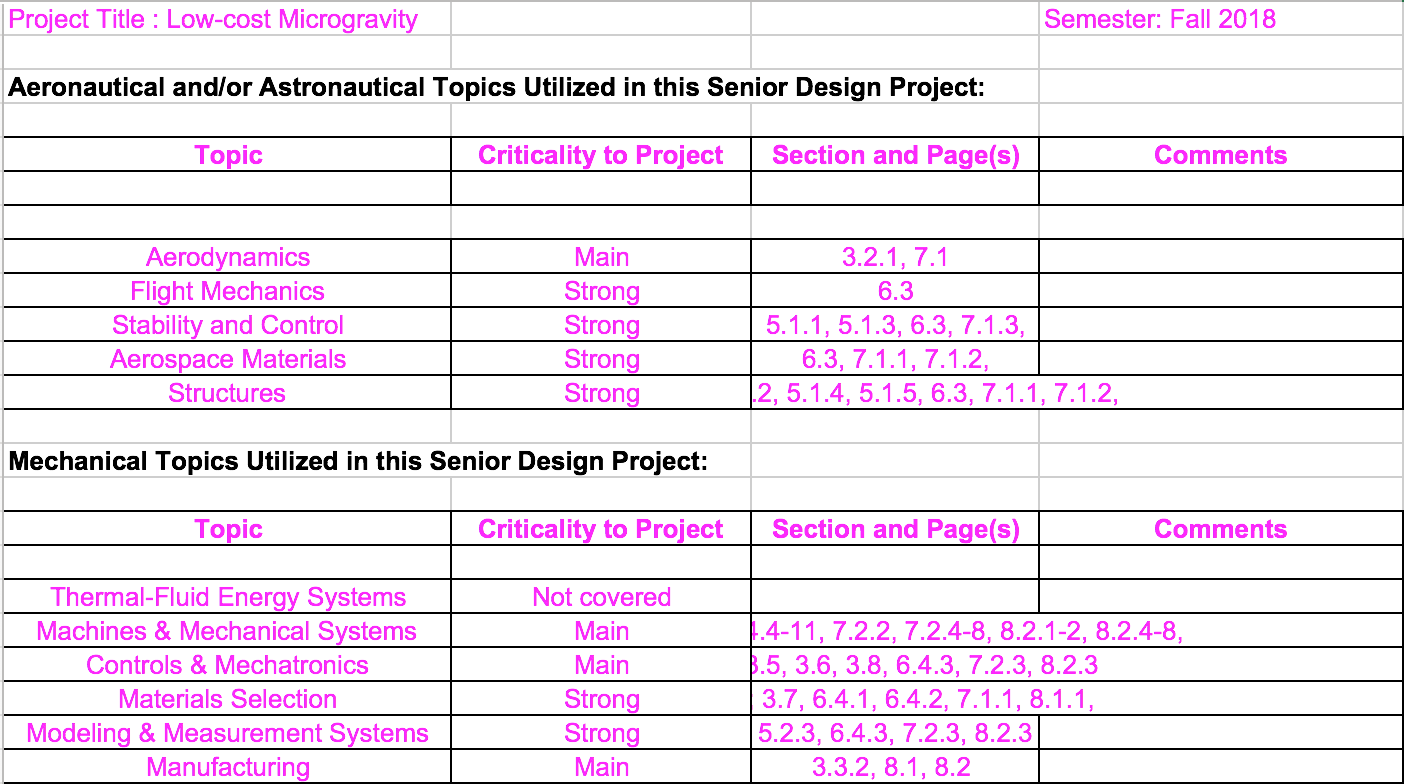
\includegraphics[width=1.0\textwidth]{Figures/DesignCompetence.png}
  \caption{\label{fig:DesignComp}MAE design competencies for ZAP-2}
\end{figure}

\newpage
\begin{figure}[ht]
  \centering
  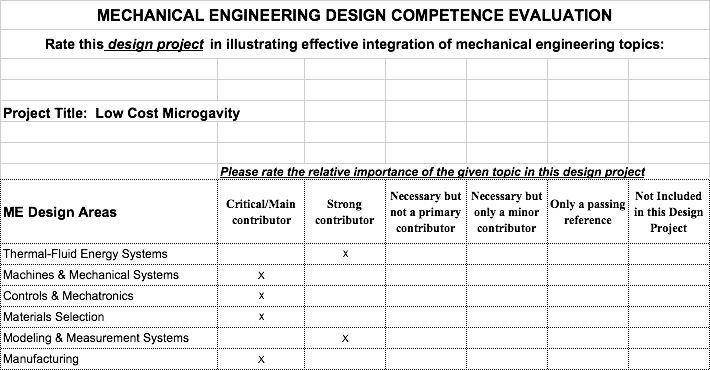
\includegraphics[width=1.0\textwidth]{Figures/Stupid2.png}
  \caption{\label{fig:Stupid2}ME Topic Competence Criticality Matrix}
\end{figure}

\newpage
\begin{figure}[ht]
  \centering
  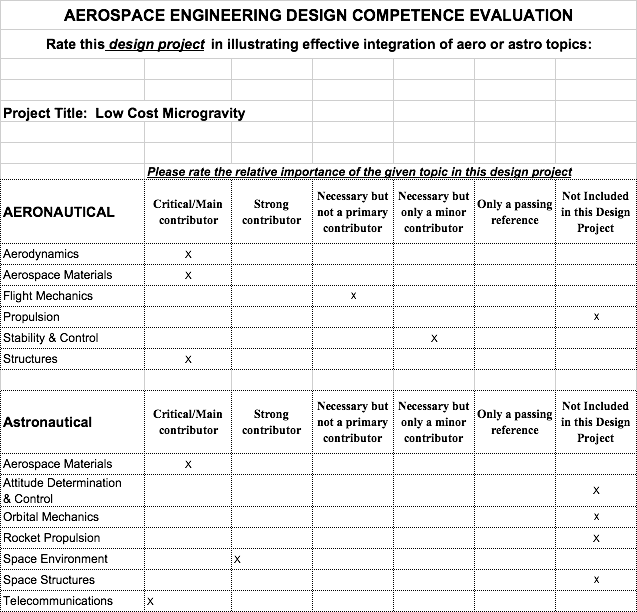
\includegraphics[width=1.0\textwidth]{Figures/Stupid1.png}
  \caption{\label{fig:Stupid1}AE Topic Competence Criticality Matrix}
\end{figure}


% ---------------------------------------------------------
% ---------------------------------------------------------
% ---------------------------------------------------------

\newpage
\bibliography{References}

% ---------------------------------------------------------
% ---------------------------------------------------------
% ---------------------------------------------------------

\end{document}

% To reference a table
[Table ~\ref{tab:NAME_OF_TABLE}]

%
% Include figures
%
\begin{figure}[ht]
  \centering
  \includegraphics[width=.4\textwidth]{Figures/Harambe.JPG}
  \caption{\label{fig:Harambe}Rest In Peace}
\end{figure}

% To reference figure
[Fig. ~\ref{fig:Harambe}]

%
% Place two figures side-by-side
%
\begin{figure}[ht]
\centering
\begin{minipage}{.5\textwidth}
  \centering
  \includegraphics[width=0.6\linewidth]{Figures/Hot-Wire_1.png}
  \caption{\label{fig:Hot_Wire_1}Hot-Wire Anemometer}
\end{minipage}%
\begin{minipage}{.5\textwidth}
  \centering
  \includegraphics[width=0.65\linewidth]{Figures/Hot-Wire_2.jpg}
  \caption{\label{fig:Hot_Wire_2}Schematic}
\end{minipage}
\end{figure}

%
% Insert Equation ( No numbering/label )
%
\begin{equation*}
	\lambda = \frac{AFR}{AFR_{stoichiometric}}
\end{equation*}

OR

%
% Insert Equation ( WITH numbering/label )
% 
\begin{equation}
	\dot{Q}=\dot{m}c_p(\Delta T)
    \label{eq:Q_heat}
\end{equation}

% To reference equation
[Eq. ~\ref{eq:Q_heat}]

%
% To add lists (with numbers)
%
\begin{enumerate}
\item ...
\item ...
\item ...
\end{enumerate}

%
% To add lists (with bullets)
%
\begin{itemize}
\item ...
\item ...
\item ...
\end{itemize} to your LaTeX file where you want your
% title page.
%
%%%%%%%%%%%%%%%%%%%%%%%%%%%%%%%%%%%%%%%%%
%\title{Milestone V}
%----------------------------------------------------------------------------------------
%	PACKAGES AND OTHER DOCUMENT CONFIGURATIONS
%----------------------------------------------------------------------------------------

\documentclass[12pt]{article}
\usepackage[english]{babel}
\usepackage[utf8x]{inputenc}
\usepackage{amsmath}
\usepackage{graphicx}
\usepackage{changepage}
\usepackage{multirow}							% Multi-rowed tables
\usepackage{booktabs}
\usepackage{xfrac}								% Slanted fractions
\usepackage{verbatim} 							% Use comment blocks
\newcommand{\minus}{\scalebox{0.75}[1.0]{$-$}} 	% Nice looking (-) signs
\usepackage{gensymb}							% Degree (^o) symbol
\usepackage[margin=1.0in]{geometry}				% Set margins at 1inch on each side
\usepackage{enumitem}							% Enumerate with whatever label
\usepackage{array}								% Define new stuff
\usepackage{subcaption}
\usepackage{wrapfig}
\newcolumntype{P}[1]{>{\centering\arraybackslash}p{#1}} 	% Vertically Centered width controlled tables
\newcolumntype{L}[1]{>{\raggedright\arraybackslash}p{#1}}
\usepackage[table]{xcolor}						% Colored cells
\usepackage{float} 								% Force float placement
\bibliographystyle{asmems4} 					% ASME Citation format
\usepackage{url} 								% Bibtex URL citations
\RequirePackage{times}      					% Loads the Times-Roman Fonts
\usepackage{longtable,tabularx}					% Load Terms & Abbreviations section
\setlength\LTleft{0pt}  						% ...
\usepackage{setspace} 							% Control line spacing

\renewcommand{\baselinestretch}{1.5} 			% Set line spacing to 1.5

\usepackage{pifont}                             % Used for creating ...
\newcommand{\xmark}{\ding{55}}                  % ... good looking 'x' signs

\usepackage{colortbl}                           % Colored columns

\begin{document}

\begin{titlepage}
{\setstretch{1.0}
\newcommand{\HRule}{\rule{\linewidth}{0.5mm}} % Defines a new command for the horizontal lines, change thickness here

\center % Center everything on the page
 
%----------------------------------------------------------------------------------------
%	HEADING SECTIONS
%----------------------------------------------------------------------------------------

\textsc{\LARGE University of Central Florida}\\[1.0cm] % Name of your university/college
\textsc{\Large Critical Design Review}\\[0.5cm] % Major heading such as course name
\textsc{\large Sponsor: Florida Space Institute, Dr. Adrienne Dove}\\[0.5cm] % Minor heading such as course title

%----------------------------------------------------------------------------------------
%	TITLE SECTION
%----------------------------------------------------------------------------------------

\HRule \\[0.4cm]
{ \huge \bfseries  Zero-g Aerodrop Project-2 }\\[0.4cm] % Title of your document
\HRule \\[1.5cm]
 
%----------------------------------------------------------------------------------------
%	AUTHOR SECTION
%----------------------------------------------------------------------------------------

\begin{minipage}{0.3\textwidth}
\begin{flushleft} \large
\emph{Authored by:} \\ 
Alvarenga, Mario \\
Boehmer, Ryan \\
Heise, Alexander \\
Kirschbaum, Justin  \\
Manley, Cole \\
Odeh, Mohammad \\
Orosco, Alec \\
Parker, Max \\
Schultz, Cody \\
Yates, Alexandra \\
\end{flushleft}
\end{minipage}
~ 
\begin{minipage}{0.4\textwidth}
\begin{flushright} \large
\hfill
Aerospace \\
Aerospace \\
Aerospace \\
Mechanical \\
Mechanical \\
Mechanical \\
Aerospace \\
Mechanical \\
Mechanical \\
Mechanical \\
\end{flushright}
\end{minipage}\\[0.75cm]

\textsc{\large Advisor: Josh Kaplan}\\[0.5cm]
%----------------------------------------------------------------------------------------
%	DATE SECTION
%----------------------------------------------------------------------------------------

{\large December 3, 2018}\\[1cm] % Date, change the \today to a set date if you want to be precise

%----------------------------------------------------------------------------------------
%	LOGO SECTION
%----------------------------------------------------------------------------------------
\includegraphics[width=0.45\textwidth]{UCF_logo.png} % Include a department/university logo - this will require the graphicx package
 
%----------------------------------------------------------------------------------------

\vfill % Fill the rest of the page with whitespace
}

\end{titlepage}

% ---------------------------------------------------------
% ---------------------------------------------------------
% ---------------------------------------------------------

% ---------------------------------------------------------
% ---------------------------------------------------------
% ---------------------------------------------------------

\section*{Executive Summary}

\indent\indent Gravity can be a disrupting factor when studying certain phenomena as it may mask the underlying physical processes that govern it. To mitigate the gravitational effects, engineers and scientists have devised controlled microgravity conditions to perform experiments that might otherwise be difficult to perform due to the distortion introduced by gravity. However, due to the high costs of performing microgravity experiments, a large population of scientists are unable to study the effects of weightlessness on certain aspects, whether it be fluid interaction, microbial growth, or material properties.

This report outlines the associated risks, methods/procedures for modeling and analysis, prototyping and testing, and development planning for each major area for the second generation prototype of the low-cost microgravity platform. Each component of the system has been broken down and evaluated for its relation, necessity and benefit to the prototype. All major findings, including changes to the original design, are described.

The first generation prototype as it currently stands consists of a platform and an aeroshell. The platform houses a motor, a reel, brakes, a set of data acquisition instruments, and a systems control unit. On the other hand, the aeroshell houses the payload containing the experiment and an additional set of data acquisition instruments. The aeroshell is attached to the platform via a tether while the platform is in turn attached to a high-altitude balloon that will deliver the system to 30 $km$ in the stratosphere. Consequent to reaching the desired altitude, the aeroshell is released and allowed to drop for a duration of +30 seconds to effectively produce approximately 25 seconds of microgravity. Upon completion of drop, the aeroshell is reeled back and the system readies itself for additional drops.

% ---------------------------------------------------------
% ---------------------------------------------------------
% ---------------------------------------------------------
\newpage

\tableofcontents

% ---------------------------------------------------------
% ---------------------------------------------------------
% ---------------------------------------------------------
\newpage

\listoffigures

% ---------------------------------------------------------
% ---------------------------------------------------------
% ---------------------------------------------------------
\newpage

\listoftables

% ---------------------------------------------------------
% ---------------------------------------------------------
% ---------------------------------------------------------

%%
%% Revision History
%%

\begin{table}[H]
\caption{\label{tab:history}Revision History}
\centering
\begin{tabular}{|c|P{3cm}|P{4cm}|P{6cm}|} 
\hline
\textbf{Version}    & \textbf{Date} & \textbf{Name} & \textbf{Reason for Changes}   \\\hline

1.0                 & 11/22/2018    & Cody Schultz  & Initial draft                 \\ \hline
1.1                 & 11/28/2018    & Cody Schultz  & Added missing figures         \\ \hline
1.2                 & 12/01/2018    & MAE Team      & Completed remaining sections  \\ \hline
1.2.1               & 12/02/2018    & Mohammad Odeh & Formatting check              \\ \hline
1.3                 & 12/03/2018    & Cody Schultz  & Final draft                   \\ \hline
1.3                 & 12/03/2018    & Mohammad Odeh & Add missing ABET Matrix       \\ \hline

\end{tabular}
\end{table}

% ---------------------------------------------------------
% ---------------------------------------------------------
% ---------------------------------------------------------

\newpage
\section*{Terms and Abbreviations}

\begin{table}[H]
\raggedright
\rowcolors{1}{gray!15}{white}
\begin{tabular}{>{\bfseries}L{2cm}L{13.65cm}}
CS  	& Computer Sciences		  							\\
EMA     & Exponential Moving Average                        \\
EOT     & End of Transmission                               \\
FSI  	& Florida Space Institute		  					\\
GPIO    & General Purpose Input/Output                      \\
I$^2$C  & Inter-Integrated Circuit (pronounced I-squared-C) \\
IMU     & Inertial Measurement Unit                         \\
IR      & Infra-red                                         \\
LED     & Light Emitting Diode                              \\
Mbps    & Mega Bits per Second                              \\
ORE     & Optical Rotary Encoder                            \\
PCB     & Printed Circuit Board                             \\
PPR     & Pulses Per Revolution                             \\
PSU     & Power Supply Unit                                 \\
PWM     & Pulse Width Modulation                            \\
RF      & Radio Frequency                                   \\
RPI     & Raspberry Pi                                      \\
SD      & Secured Digital                                   \\
SMA     & Simple Moving Average                             \\
SoC     & System on Chip                                    \\
SOH     & Start of Heading                                  \\
%... 	& ...  												\\
\end{tabular}
\end{table}

\begin{table}[H]
\raggedright
\rowcolors{1}{gray!15}{white}
\begin{tabular}{>{\bfseries}L{2cm}L{13.65cm}}
$\mathbf{a}$		& Acceleration 							\\
$\mathbf{A}$		& Area      							\\
$\mathbf{C_D}$		& Drag Coefficient						\\
$\mathbf{C_g}$		& Center of Gravity						\\
$\mathbf{C_p}$		& Pressure Coefficient					\\
$\mathbf{g}$		& Acceleration Due to Gravity (9.8 m/s)	\\
$\mathbf{\Phi(t)}$	& Heaviside Step Function				\\
$\mathbf{I}$		& Moment of Inertia						\\
%... 	& ...  												\\
\end{tabular}
\end{table}
% ---------------------------------------------------------
% ---------------------------------------------------------
% ---------------------------------------------------------
\newpage
\section{Introduction}

\begin{comment}
Review and update material from the Mid Term Report. This section should concisely address the following issues and point to an appropriate document or Appendix containing detailed information as needed:
•	History behind the project
•	Major end users’ needs and/or problem to be addressed (Present detailed customer requirements in an Appendix.)
•	Justification (benefits) for pursuing the project (worth for solving or improving)
This section also contains a summary of report sections.
\end{comment}

\indent\indent Microgravity is most simply defined defined as a very low acceleration typically compared as a minute relative percentage of Earth's gravity of approximately $9.81 m/s^@$. The prevailing approaches used to achieve microgravity conditions consist of parabolic flights, drop towers, and suborbital flights. Notwithstanding, they all suffer from severe limitations in one form or another, not to mention the exorbitant price tags that are often associated with the operation. For instance, although parabolic flights produce a decent duration of microgravity conditions – up to 25 seconds – they are usually limited to low quality microgravity conditions \cite{Novespace}. Furthermore, the duration of microgravity conditions for experiments performed in drop towers is usually limited by the height of the shaft where the tower is erected. In addition, the time required to evacuate air from the tower to reduce viscous forces is rather long and is a time-consuming process. Lastly, suborbital flights, such as the sounding rocket, can produce 12-13 minutes of microgravity \cite{GAC}. However, it is fairly expensive and campaigns that offer to deliver a payload to a suborbital path are not readily available. Costs to researchers are further inflated when the system requires end-users or research surrogates to manually operate their experimental payloads in person, such as on the International Space Station.

The previously stated limitations are what motivated the design of our system as it aims to reduce, if not eliminate, them. Starting with cost, system components are chosen from mostly off-the-shelf parts, reducing costs required to manufacture highly specialized parts and equipment. In addition, duration limits are also countered by dropping the system from a very high altitude of 30 km. Furthermore, the microgravity quality is theorized to be within the magnitude of $10^{\minus 3}g$. Lastly, the system is designed to be semi-autonomous and capable of carrying out mission critical operations independent of human interaction, allowing for multiple drops within a single flight. No other previously mentioned approach has the combined benefits of the system to be developed.

As noted, our system aims to produce a viable, low cost alternative microgravity solution that can be readily used by scientists aiming to perform experiments in microgravity conditions. Prior to our teams work, a first-generation of previous senior design group at the University of Central Florida produced several innovative concepts that were meant to test the feasibility of such a system. The work of these first-generation teams ranged from addressing subsystem designs to producing a small-scale working prototype. Our second-generation work is largely on the concepts and overall design architecture provided by these earlier teams. Our contributions have been to optimize the design for longer duration flights and produce a working prototype capable of demonstrating those performance requirements. 

This project was created and funded by the Florida Space Institute (FSI) with the guidance of Dr. Adrienne Dove from the University of Central Florida to increase accessibility of testing their microgravity research experiments. However, this project is capable of serving a much larger customer base of research organizations conducting microgravity research experiments such as the National Aeronautics and Space Adminstration (NASA), the European Space Agency (ESA), etc. It could also hold value to commercial entities, such as MadeInSpace or TransAstra, interested in the impacts of microgravity on future technology, including deep space exploration, asteroid mining and the colonization of other planets.

% ---------------------------------------------------------
% ---------------------------------------------------------
% ---------------------------------------------------------

\section{Project Objectives \& Scope}

\begin{comment}
This section contains both long term objectives and the planned semester objectives. Provide a bullet list of the objectives for this semester.  Focus on final outcomes, not intermediate steps. Do not include task assignments in this section. The objectives should be understandable by themselves.  However, you can follow the objectives with a statement of scope to clarify what you planned to do (in scope), and that you planned to not do (out of scope). 
\end{comment}

\indent\indent The ZAP-2 team primary directive to provide a system capable of meeting the customer requirements defined in Appendix \ref{customer_reqs}. To summarize the requirements, we are to produce a dynamic, mechanical system capable of repeatedly providing high-quality ($< 10^{-3}$ g\'s) microgravity conditions for an integrated experimental payload the size of a middeck locker. The system must be able to operate autonomously in stratospheric conditions. To meet these customer requirements we have developed our own series of system level requirements defined in section ~\ref{sys_reqs}. To produce this system and meet these requirements we have developed a list of long-term and semester-long objectives that we've used to guide our efforts. Long-term objectives describe the absolute end goals of this project well beyond the conclusion of our contributions through the senior design course. Semester long goals on the other hand outline the goals that we've worked to achieve throughout and up to the conclusion of this course. They're the goals that our team has worked to meet and deliver. 

\subsection*{Long-term Objectives}

\begin{itemize}
    \item Produce a flight-ready system capable of providing super-high-quality microgravity conditions (on the order of $< 10^{-6}$ g's) for drop durations of up to 25 seconds.
    \item Create a system capable of repeated drops ($> 10$ drops) in a single flight.
    \item Produce a system capable of operating semi-autonomously that allows for user supervision and intervention. 
    \item Fabricate a system capable of operating in stratospheric conditions for hours on end while also being robust enough to endure the dynamic forces throughout a mission while requiring as little maintenance as possible.
\end{itemize}

\subsection*{Semester objectives}

\begin{itemize}
    \item Design and manufacture a potentially flight-ready system capable of providing high-quality microgravity conditions (on the order of $< 10^{-3}$ g's) for drop durations of up to 9 seconds.
    \item Perform critical design analysis on the system concepts to mathematically demonstrate system capabilities.
    \item Identify and utilize affordable, practical manufacturing techniques to create said system and future systems. 
    \item Demonstrate system capabilities by either demonstrating integrated system functionality for up to a 2 second drop or demonstrate individual subsystem capabilities proving their capability to meet their defined performance standards. 
\end{itemize}



% ---------------------------------------------------------
% ---------------------------------------------------------
% ---------------------------------------------------------

\section{Assessment of Relevant Existing Technologies and Standards}

\indent\indent Prior to the conception of our system design our team was tasked with researching existing technologies, systems, hardware, and software that currently provides analogous capabilities or could potentially contribute to our future design. This research is captured in the succeeding documentation. 

Please note, as previously stated, the work of our team is largely based on the architecture provided by the first-generation senior design groups. Therefore, the following details are provided with specific context to the subsystem in which the researched technologies are associated with. 

\subsection{Microgravity Research Platforms}

\indent\indent Today there exists three main methods for achieving microgravity conditions for experimentation, which include drop towers, parabolic flights, and orbital platforms. Drop towers, as their name implies, consist of a chute or tower through which a payload is dropped. The length of microgravity and quality is dependent on the height of the tower and the air resistance the payload experiences. To achieve quality microgravity conditions, drop towers range from a few meters to over one hundred meters and the tower may or may not have air evacuated to create vacuum conditions. Parabolic flights allow experimenters to place their payload into an airplane that then flies through a series of parabolic arcs that create microgravity conditions lasting on the order of tens of seconds. Lastly, orbital platforms such as cubesats or the International Space Station, allow for long term and high-quality microgravity conditions but may be prohibitively costly. Beyond these three main methods also existences unique experimental system, which are often less utilized and include the Japanese Aerospace eXploration Agency's (JAXA) Balloon-based Operation Vehicle (BOV) and quadcopter based paylods. Of all these techniques, our experiment will most closely resemble the JAXA's BOV system.

% ---------------------------------------------------------

\subsubsection{Drop Towers}

\indent\indent A drop tower is, as the name implies, a vertical column inside of which a payload is dropped. During free-fall the payload is expected to experience some level of microgravity conditions. The enhance the quality of microgravity, the vertical column may be evacuated of air to decrease or completely eliminate the drag force the falling payload experiences as it plummets that would otherwise tarnish the quality of microgravity. Drop towers can range from simple open air design being only several meters high to highly complex systems over 100 meters in height.

NASA has two drop towers both located at the Glenn Zero Gravity Research Facility located in Brookpark, Ohio. The largest of the two is a 132 meter tall vacuum chamber tower capable of achieving gravitational accelerations of less than $10^{\minus 5}$ G's for durations of 5.18 second \cite{NASA0G}. It is NASA's premier microgravity drop tower used for studying the effects of microgravity on physical phenomena such as combustion and fluid physics, to develop and demonstrate new technology for future space missions, and to develop and test experiment hardware designed for flight aboard the International Space Station or future spacecraft. The vacuum chamber itself is 142 meters tall and is capable of achieving pressures on the order of $0.05 torr$. Operational procedure begins with a crane lifting the payload to the top of the tower. Air is then evacuated from the chamber. Once the chamber is evacuated the release sequence is initiated by remotely fracturing a specially designed bolt allows the experiment to begin free fall. During the drop the experiment operates autonomously with all experiment power, data acquisition, and control functions located on the vehicle. After falling for approximately 5 seconds the experiment vehicle is stopped in the decelerator cart, located at the bottom of the chamber. The decelerator cart is filled with $3 mm$ diameter expanded polystyrene beads that dissipate the kinetic energy of the $2500 lb$. experiment vehicle. Maximum velocity at the point of deceleration approach $50.5 \sfrac{m}{s}$. The vehicle decelerates from its peak velocity to a standstill in $4.6 m$ of of expanded polystyrene and experiences a peak deceleration rate approaching 65 g's \cite{NASA0G}.

The second drop tower at NASA Glenn Research Center is an open-air 24 meter chute capable of achieving 2.2 seconds of microgravity conditions on the order of $10^{\minus 3}$ G's \cite{JAXALabs}. Because the experimental payload is open to the air, it is also subject to the drag forces due to atmosphere. To minimize these effects researchers employ a drag shield which increase the aerodynamic performance of the payload allowing for diminished drag forces. The payload itself is isolated from the drag shield and falls 19 cm relative to the structure, allowing for optimized microgravity conditions. The payload and shield are then stopped by an airbag deployed at the bottom of the tower \cite{NASADropTower}. 

The Bremen Drop Tower located at The Center of Applied Space Technology and Microgravity (ZARM) in Bremen, Germany, has the world's longest duration microgravity drop tower. The facility features a 120 meter vacuum chamber that can be configured to either drop payloads from the top of the tower or launch them on a catapult system from the bottom of the tower, effectively doubling the duration of microgravity. In the traditional configuration the payload capsule is pulled up to a height of 120 meters to the top of the drop tube and then released. After 4.74 seconds the capsule is decelerated in a unit filled with polystyrene pellets, much like the setup at NASA's Glenn Research Center. Vacuum pumps evacuate the chamber of air to pressure of one ten thousandth of the normal air pressure \cite{ZARM}. In catapult mode a pneumatically driven launch system location at the base of the tower accelerates the capsule to speeds of approximately 168 kilometers per hour in just 0.25 seconds. The velocity and launching force is uniquely calculated for each experiment in order to provide microgravity conditions for up to 9.3 seconds. The same deceleration unit quickly replaces the launch system at the base of the tower ensuring a safe landing for the capsule \cite{ZARM}. 

% ---------------------------------------------------------

\subsubsection{Parabolic Flights}

\indent\indent Parabolic flights, which offer approximately 20-25 seconds of microgravity for 25-30 consecutive parabolas, are currently priced at \$38,500 for a single research team [5]. They offer researchers the ability to test their experiment payloads repeatedly while being present to operate them. Payloads can be either rigidly attached to the plane or be disconnected from their storage unit during flight and free float about the cabin during the periods of microgravity- something unique to parabolic flights. Microgravity is achieved by angling the plane upward, experiencing approximately 1.8 g's,  then smoothly arcing and angling downward, creating the weightless sensation. The actual gravity experienced on parabolic flights is not exactly 0 g, but more accurately $0 \pm 0.01$.

An advantage of parabolic flights is the large number of parabolas flown. Having a large number of parabolas and, consequently, multiple intervals of microgravity, allows researchers to operate there experiments 20-30 times, ensuring more accurate and usable data. During flight, if the experiment becomes non-operational, researchers have the ability to make adjustments to hopefully restore all function and run it during the next parabola. This ties into another advantage of being able to fly onboard with your payload. During other methods of simulating microgravity researchers aren't able to operate their experiment themselves, but rather it needs to be fully automated. A third advantage of parabolic flights is the severity of g-forces experienced by the payloads is a maximum of 2 g's [16]. This is much lower than that of drop towers and suborbital rockets, reducing damage on experiments and offering more design flexibility.

A major disadvantage of parabolic flights is the frequency of which they occur. Currently, ZeroG offers research flights twice per year. These dates are set by the company far in advance, and are subject to change without warning due to weather disturbances or occupied airspace. Another disadvantage is the environment itself- parabolic flights require human interaction with the payloads, increasing the probability for human error. An additional disadvantage is the quality of microgravity. Microgravity is defined as $10^{\minus 9}$ g, but parabolic flights produce approximately 0.01 g's. Additionally, the gravity during those 30 seconds can fluctuate, invalidating the testing done.

% ---------------------------------------------------------

\subsubsection{Orbital/Suborbital Platforms}

\indent\indent For longer durations of microgravity, researchers may look to suborbital and orbital platforms. By definition, a suborbital space flight operates at an altitude higher than $100 Km$ (328,000 ft) above sea level. This altitude is classified as the Kármán line, chosen by the Fédération Aéronautique Internationale; the USAF and the FAA consider a lower altitude of $80.47 Km$ (264,000 ft) as the altitude to qualify as space flight. These options offer cleaner microgravity for longer periods of time, but come with their own unique disadvantages. 

Blue Origin's New Shepard rocket provides approximately 3 minutes worth of clean microgravity and can accommodate payloads up to 50 lbs. They provide vehicle telemetry data, electrical power, cameras, data storage and robust control systems. Blue Origin has flown multiple payloads, including four from UCF's Physics Department (COLLIDE). Virgin Galactic's SpaceshipTwo is still undergoing testing, but has begun reserving spots for research payloads upon completion. SpaceshipTwo will have a 0 g coast phase lasting approximately 4 minutes.

Disadvantages associated with suborbital flights include the severe vibration experienced by experiment payloads, autonomous operation, and varying interface requirements between companies. Vibrational effects are substantial on suborbital flights. SpaceshipTwo expects to experience a maximum of 3.8 g during the boost phase, and a maximum of 6 g during deceleration \cite{L2}. Because of this, research team members must thoroughly prove way in advance via simulations and testing that their payloads are capable of undergoing those forces while maintaining their overall safety levels. Autonomous operation and varying interface requirements are also a disadvantage since payloads need to be manipulated depending on the company they are flying with. Blue Origin offers signal triggering for payloads, as well as a detailed flight profile, while Virgin Galactic requires all triggering to be handled by the researcher teams.

Another major disadvantage of suborbital flights is the infrequency of flight. Because these flights are so costly, they are booked more than a year in advance, require constant communication between the research team and flight company, and a series of paperwork milestones to ensure adequate payload operation and safety. Because of this, flights are often delayed anywhere from 3 months to over a year, depending on the circumstance. Additionally, this may not be a long term solution for researchers since the end goal of these companies is space tourism- experiment payload lockers will be replaced by paying human passengers wanting to become astronauts.

The most well-known orbital platform is the International Space Station (ISS). The ISS was developed by a multitude of nations with the purpose of serving as a shared research platform. The research aboard the ISS is categorized into 3 sections: NASA research, ISS International Laboratories/CASIS, and International Partners. There are 6 phases associated with operating a research payload aboard the station, resulting in a lengthly approval process for all payloads. Today, the only American company to visit the ISS and deliver science payloads is SpaceX via its CRS-8.

While the ISS offers the longest duration of microgravity for research experiments, there are many disadvantages associated with this particular method. First, and most obvious, the selection process is the most selective. While the station houses an extensive number of experiments, the approval process is highly competitive. The cost of sending a research payload to the ISS is also the highest of all methods of testing, requiring funding from NASA grants -or the like- to fund this method of testing. Testing aboard the ISS is the ideal method for a majority of experiments due to the exponentially longer duration of clean microgravity, but is unrealistic for most.

% ---------------------------------------------------------

\subsubsection{JAXA's BOV}

\indent\indent The Japanese Aerospace Exploration Agency’s (JAXA) Institute of Space and Astronautical Science has developed a Balloon-based Operation Vehicle (BOV) that is a link between terrestrial drop towers and the innovative concept our group is working on. The system consists of a high-altitude balloon that lifts a $700 Kg$ payload to approximately $40 Km$ where the BOV is then disconnected and plummets for $20$ to $30 Km$ before deploying parachutes to slow the descent into the ocean \cite{JAXALabs}. The BOV achieves approximately 30 seconds of microgravity as low as 10-4 \cite{JAXALabs}. The BOV itself was designed to be extremely aerodynamic, which resulted in a structure approximating that of a missile or rocket. The experimental payload was then housed inside of this structure where it remained for the entire duration of the flight.

JAXA's BOV was a multi-generational project with each subsequent iteration building on the successes and failures of the previous iteration. The original design incorporated their experimental payload into the BOV by rigidly securing it to the structure. This allowed the payload to remain safely fixed with the caveat that it experienced any vibrational forces or turbulence that the BOV experienced during free-fall. Later generations incorporated one-dimensional and three-dimensional drag-free systems that helped to isolate the payload from the aeroshell and thus insulating it from the forces that would bring the payload out of quality microgravity. The one-dimensional system illustrated in [Fig. ~\ref{fig:JAXABOV.png}] consisted of a simple rail system that allowed the payload to move independently from the BOV in the vertical direction. Cold gas thrusters were also incorporated into the BOV to accelerate the capsule when drag forces began to disturb the BOV/payload displacement. Microgravity conditions lower than $10^{\minus 3}$ g's were achieved for a duration of approximately 30 seconds \cite{JAXAResults}.  The three-dimensional drag-free system, also illustrated in [Fig. ~\ref{fig:JAXABOV.png}] consisted of a spherical payload fixed to the BOV via tethers. The BOV then used 60 cold gas thrusters to keep the outer structure clear of the free-falling payload contained within it. Laser displacement sensors between the two track clearances due to external drag forces. Microgravity conditions up to $10^{\minus 3}$ G's were experienced for durations of only 8 to 10 seconds \cite{JAXAResults}. A tri-axial accelerometer (Silicon Design Inc. Model 2440) was used to track multi-dimensional acceleration to verify and track microgravity conditions. A RHOM-Riken R2-Micro datalogger with a $900 Hz$ sampling rate was used to capture sensor data \cite{JAXALabs}. Temperature and humidity were also captured for climate control to keep the payload within operating conditions.

\begin{figure}[H]
  \centering
  \includegraphics[width=.4\textwidth]{Figures/JAXABOV.png}
  \caption{\label{fig:JAXABOV.png}Drag-free external force isolation systems for payloads in JAXA's BOV vehicle.}
\end{figure}

A major advantage of the one-dimensional drag-free system is that it allowed for a much larger payload and provided almost four times the duration of quality microgravity conditions. The JAXA BOV system most closely approximates our design and provides a wealth of useful information that will influence our design and procedures. Most notably, the vibrational damping/disturbance rejection system, launch procedures, and control technology should all be carefully considered for integration into our design. 



% ---------------------------------------------------------

\subsection{Aeroshell}

\subsubsection{Geometry}

\indent\indent For the aeroshell, the main goal of the geometry is to decrease the amount of drag force and initial pressure while dropping through the stratosphere to achieve microgravity. A symmetrical airfoil is chosen because it will not produce a significant amount of lift and it decreases the drag coefficient during the drop. The specific symmetrical airfoil chosen is a hydrofoil, which has the main purpose of lifting a boat's hull above water. The hydrofoil decreases drag and also gains speed on its travel path. There are many other airfoils that are candidates, such as, aerobatic and NACA airfoils. The hydrofoil is not a conventional airfoil that can be seen on a general aircraft wing or tail. Hydrofoils tend to have a sharper trailing edges, which is similar to subsonic flight airfoils.

Optimization of airfoils to decrease drag is the current technology to produce better and more efficient airfoils for various uses. These airfoil uses range from turbines, turbofans, propellers, and airliners. The optimization process tends to yield results for high lift to drag ratio. The process can use a Matlab code and call another program within the code to retrieve different airfoils and "mutate" the airfoils through each iteration. The called program tends to be XFoil, which is a program for design and analysis of subsonic isolated airfoils. The different methods used within the optimization codes to parameterize the airfoils are PARSEC, CST, and a variant of Karman-Trefftz. For the purpose of this chosen symmetric airfoil, the desire is to have a low drag and to minimize any lift that would occur during flight. There are little to no codes created for symmetric airfoils with the main purpose of decreasing the drag coefficient. However, a code by Zheng Wang using Genetic Algorithm optimizes symmetrical airfoils \cite{optimize}. This optmization code also uses XFoil as a program to create "mutated" airfoils and to iterate the airfoils until the optimizer has converged.

% ---------------------------------------------------------

\subsubsection{Payload}

\indent\indent To ensure the system is versatile enough to accommodate a wide variety of microgravity payloads, the internal structure of the aeroshell will be designed to the specifications of a middeck locker. The three designs considered for housing the payload were a static attachment, an linear rail system, and a 3 dimentional isolation system. The static attachment would be the simplest to implement but the most likely to lower the quality of microgravity for the payload. The linear rail would improve the quality of microgravity considerably over a static attachment, but would also greatly increase complexity and modes of failure. A 3 dimentional isolation system, similar to that employed by JAXA \cite{JAXALabs} would allow for the greatest fidelity of microgravity but also the greatest complexity. 

The standard middeck locker was the payload size specification requested by the intended user of the microgravity platform. The aeroshell will use a standard middeck locker to contain the payloads, and mount any payload hardware to a standard adaptor plate. This simplifies the design requirements of the aeroshell internal hardware because whichever isolation technique is used, the payload will always be a standard size and shape.

The choice of mounting and isolation drives many subsequent design requirements. A simple attachment would minimize the greatest diameter of the aeroshell. The aeroshell would need only to fit the width of the middeck locker at the top and bottom panels. A linear rail would increase the aeroshell diameter because the aeroshell would need to accommidate the width of the middick locker at both the top and the bottom of the rail system. To maintain the chosen aeroshell shape, the length and diameter of the aeroshell would increase significantly. This holds true for the 3 dimentional isolation system as well. The simple attachment is the recommended method for the current iteration of the project.

The two more complicated options also introduce the need of a control system. To ensure the benefit of the linear rail is applied to every drop test, the aeroshell would need a method to raise the payload within the aeroshell, hold the payload at the top of the rail, but still allow the payload to slide along the rail unimpeded. The recommended method to achieve this is to raise the payload with a pushing linear actuator until the payload reaches the top, engage an electromagnet at the top of the rail to hold the payload in place while the linear actuator retracts, then simultaneously release the electormagnet and the aeroshell as a whole. This system is strongly recommended for future iterations of this project, but ultimately out of the scope of the current iteration of the aeroshell.

% ---------------------------------------------------------

\subsubsection{Latch}

\indent\indent Since the aeroshell is to be manufactured in halves it warrants a way to align and fix them together. Many candidates were considered such as case latches (used in heavy duty road cases), snap latches (used in many flexible case enclosures), and hook and eye latches. Ultimately, it was decided to incorporate roto-lock coffin latches into the design for their strength, holding capacity ($750 kg$ each), and ease of use. With one hex key, the coffin latch can be engaged or disengaged to join or release the two halves in seconds; however, since it is originally designed as a “latching biscuit joint” an additional aluminum part will need to be machined and bonded to the aeroshell to make use of it as an internal latch. Also, additional carbon fiber layers can be applied during fabrication to thicken and increase strength of the attachment points to avoid pull-through and shear-out failure conditions at the bolt interface. Finally, if necessary, a small scoop could be installed over the bolts to help alleviate the drag of the exposed metal. Although the aeroshell will be directly fastened to the internal structure in separate locations, having the coffin latch will speed up assembly and provide a redundant system to ensure the shell stays closed and aligned.

% ---------------------------------------------------------

\subsection{TUMBR}

\subsubsection{Tether}

\indent\indent The material of the tether must be lightweight, durable, and resistant to atmospheric conditions that may weaken the functionality. The best solution found for this material is Spectra, developed by Honeywell. The material is known to be one of the world’s strongest and lightest man-made fibers, and has been implemented by the Department of Defense (DOD) for military and police applications. Spectra is fifteen times stronger than steel, more durable than polyester, and resists corrosion, chemicals, and abrasion, making it an ideal choice for repeated impact and atmospheric conditions. The disadvantages found with this material are the high cost and lead time. The material chosen by the previous team for the scaled model, however, was Kevlar, due to its high strength, low creep, good temperature performance, and low stretch \cite{trt}. For this iteration of the project we will be moving forward with Spectra by Honeywell and proceeding with a 9 second drop. A major constraint of the tether will be the diameter and weight, which was allocated to a max of $5 mm$ and $100 Kg$ by the previous team. By scaling up the project to perform a 9 second drop, the length of tether needed will be approximately 600 km.

% ---------------------------------------------------------

\subsubsection{Unit}

\indent\indent The platform structure will house the tether/reel and tether guide, braking system, and dual motors. The previous iteration of the project constructed the platform frame from 80/20 Aluminum. This material is commonly used in engineering applications due to the low cost, high strength to weight ratio, availability, and ease of machining. 80/20 is 2x stronger than steel and approximately one third the weight, offering a unique opportunity for frame applications. This material is also much less corrosive than comparable metals, and keeps its shape when exposed to temperature changes- unlike steel. 80/20 also comes in a T-slot design, which makes adjusting attachment points and altering designs much more feasible since those attachments are not permanent. As a result, these pieces can be re-purposed at the conclusion of a project rather than discarded- reducing overall costs. 

% ---------------------------------------------------------

\subsubsection{Motor}

\indent\indent The motors used in the prototype for both applications were AmpFlow E30-150 24-volt DC motor, which could operate between 12-36 volts, have $5 Nm$ of torque, produce around $750 W$, and can produce maximum RPM of $8700 RPM$. Calculations showed that $8.4 Nm$ of torque would be required to lift the aeroshell, however the motor on the system for reeling the payload back onto the spool can only produce $5 Nm$ of torque. Through a gear reduction of 9/32, a max torque of $17.78 Nm$ would be produced by the motor and would meet the required torque to raise the payload.

Three types of electric motors were considered for the system: AC, brushed DC and brushless DC. AC motors are powered by an alternating current that runs through a stator, producing a magnetic field. The previous team opted not to use AC motors due to their significantly higher cost and slightly increased performance. DC motors are powered via a direct current and are much more feasible at higher altitudes. A set of magnets are positioned within the stator and the armature has wire wrapped around an iron core. Depending on whether the motor is brushed or brushless determines the operation; brushless motors use a controller to activate/deactivate each coil. Brushed motors transmit power through brushes to energize the wires at specific times. Brushed DC motors require more maintenance and have a shorter life than brushless DC motors, but offer reduced initial costs and better control.

% ---------------------------------------------------------

\subsubsection{Brake Systems}

\indent\indent Braking systems can be complex to manufacture, so the previous team decided it was best to design the brake system with items which could easily be obtained from off-shelf items and replaced easily if necessary. A simple friction-based caliper and rotor setup was designed to attach to the platform and the shaft of the system. Friction based braking is a very reliable and predictable way to slow down an object, with the only major downfall being the replacement of the friction material (brake pads or rotor). The caliper and rotor on the first generation prototype were both fashioned from a Honda Fit and calculations proved that a deceleration was more than enough to bring the aeroshell to a safe halt. A linear actuator was connected to the master cylinder of the braking system so the controls and instrumentation team could precisely apply pressure when coupled with a microcontroller.

The braking system on the prototype is currently non-functional due a tilt in the rotor and uneven caliper mounting when assembled. The slight tilt in the rotor coupled with an uneven caliper mount produces a non-uniform deceleration with heavily increased frictional forces. The increased friction caused by this manufacturing error prevented the previous team from full integration testing.

The previous team used an iron rotor fashioned from a Honda Fit for their frictional braking system. The rotor on the system will be rotating approximately upwards of 5,000 revolutions per meter (RPM) for a nine second drop which leads to a large heat flux and large shear force when braking is applied. Iron rotors are heavy and known to deform and warp at high temperatures and loads. These are very undesirable traits when weight, reliability, and repeatability are three important factors dealing with this project. Carbon-ceramic brakes are used in high end cars because of the great response in both wet and dry conditions, the high durability, the low weight, resistance to corrosion and are characterized by having an extremely low deformation under high temperatures.
% * <jkirschbaum1992@gmail.com> 2018-04-16T00:41:11.304Z:
% 
% " Because of these inherent traits of iron high performance cars turn their eyes to another material which will perform much better under stressful environments."    
% 
% Wat?
% 
% ^.

Future modifications made to the braking system will include the addition of an electromagnetic braking system. The two systems will function as a combined braking system- the electromagnetic initiating first to slow the shaft to an optimal angular velocity, at which point the frictional system will begin operating to slow the speed to zero. Electromagnetic braking systems are currently used in high velocity applications, such as trains and roller coasters. A major disadvantage is the proportional braking force and velocity, meaning the system loses efficiency as the velocity decreases. For this reason a frictional system will remain a part of the design. The decreased velocity when the frictional system begins will extend the life of both the brake pad and rotor.

% ---------------------------------------------------------

\subsubsection{Reel}

\indent\indent The reel has four main components: the shaft, tether walls, frame, and bearings. The shaft, tether walls and frame were constructed from steel, while the bearings were made from stainless steel. The frame was fabricated with 2” square 80/20 bars welded at the corners with an x-brace design at both ends to maximize strength and minimize weight.  In the center, a cylindrical shaft holds two 10” diameter discs which acts as a housing to hold the tether in place on the shaft. To help release the tether from the reel, two disks were fabricated to clamp the tether and pull it off the reel at $2107 RPM$.

A major consideration for the reel includes a tether guide to ensure no additional forces are acting on the tether and reduce overall vibration on the aeroshell. By adding this mechanism to the platform, the tether will cleanly unroll and respool each drop without tangling or knotting. Previous designs were constructed for a functioning tether guide, but their interface with the overall platform was not ideal. Current mechanisms exist and will be implemented in the design.

% ---------------------------------------------------------

\subsection{Controls \& Instrumentation}

\indent\indent The development of the controls and instrumentation module of the second generation prototype was distributed amongst the MA team and the CS team in order to allow the MA team to focus on developing the mechanical and structural components of the system. However, the MA team was given the task of choosing the appropriate sensors and developing the required code to interface them with the controls system that is to be provided by the CS team.
Certain requirements need to be met for the the successful trial runs and meaningful data collection.

\begin{enumerate}
\item Controls unit must be able to interface with all the sensors on board.
\item Sensors need to relay data back to the controls unit for logging and data storage.
\item Controls unit and sensors must both be able to operate under harsh environmental conditions.
\item A proper calibration routine must be performed to reduce the effects of ambient noise.
\item Sensors must be repeatable and of high fidelity.
\item Must be cost-effective in order to fulfill the imperative of this mission.
\item Must be feasible to integrate within the system
\end{enumerate}

The conceptualized controls and instrumentation module layout as envisioned by the CS team is presented in [Fig. 3].

\subsubsection{IMU}

\indent\indent The IMU must be able to record the acceleration of the system as it is being dropped. In order to gather high quality data, the signal must have a low noise density, this can be achieved by actively filtering the data software wise in conjunction with the addition of an appropriate capacitor near the signal line of the breakout board of the sensor. Furthermore, the IMU must be able to record accelerations of at least $10^{−3} m/s^{2}$ for the data to be meaningful. Being able to achieve such values heavily rely on the resolution and sensitivity of the sensor, and as such, the IMU must have a resolution and sensitivity that allows it to measure and record accelerations in the range of $10^{−3} m/s^{2}$.

\subsubsection{Temperature Sensors}
\indent\indent As with the IMU, the temperature sensor must be able to monitor and record the experimental environment conditions and possibly monitor the system’s condition. Such data is vital for the experimenter as will as for the operation of the system. For instance, a temperature sensor could be employed to monitor the motor’s temperature. In case the motor overheats for any reason, the temperature sensor could signal the control unit to halt the next drop until the motor cools down.

\subsubsection{RPM Measurement Device}

\indent\indent The monitoring of the RPM at which the tether is being ejected is one of the most important parts of the experiment as the ability to achieve microgravity is dependent on the team’s ability to reduce all the forces acting on the aeroshell. The role of the RPM measurement device is to signal the motor to run at a higher speed such that it unwinds tether from the spool at a slightly faster rate than that of which the tether is being ejected from the system. For the RPM measurement device to be effective, it must be able to read and register RPMs of +5,000 as per the preliminary calculations. To that end, two types of measurement devices can be used; a tachometer or a rotary encoder. However, it must be noted that for the purposes of prototype validation a rotary encoder is to be used while a tachometer is to be used for the full-scale system for reasons that are discussed in section ***5.5.3***.

\subsubsection{Controls Unit}

\indent\indent The controls unit can be thought of as the central hub of the system where everything has to go through and where all the commands are issued and executed. In order to fulfill this purpose, the controls unit must have ample GPIO pins to interface all the sensors and peripherals. Moreover, the controls unit must have adequate processing power to perform all the calculations and data storage operations in real-time.

\indent Previous teams opted for the use of the Arduino MCU in parallel to a RPi running the Raspbian Jessie OS. This added a layer of complexity to the controls and instrumentation module as data had to go through two hops before reaching its final destination. This can be mitigated by the use of a RPi running a minimal OS known as DietPi that is light on resources, leaving said resources available for the interaction between the RPi and the remainder of the system [24]. Additionally, the RPi can be overclocked allowing for a higher frequency effectively reducing lag between the moment at which data is received, processed, and an appropriate command is issued.

\subsubsection{Programming Language}

\indent\indent A programming language must be used to produce a set of instructions that can be used to produce various kinds of output and implement specific algorithms. The choice of an appropriate language is important as it determines whether the controls and instrumentation module will operate in real-time or not.

\indent Two classes of programming languages exist; interpreted and compiled languages. Interpreted languages, as the name implies, are interpreted at run-time and everything is processed as the interpreter reads a line of code. On the other hand, compiled languages assemble the code prior to execution and converts it to a lower-level form in which the program can be executed, reducing a level of abstraction found in interpreted languages.

\indent Previous teams had used a mix of both languages on the first generation prototype. As an example, all the MCU’s were programmed using C/C++, a compiled language, and all the RPi’s were programmed using Python, an interpreted language. For the sake of continuous improvement, the second generation will be using C/C++ for all programming purposes as it offers unparalleled execution speeds when compared to an interpreted language such as Python, allowing for near real-time operation.

\subsection{Power Supply Unit}

\indent\indent Lastly, no previous intensive work was aimed at the power supply and distribution units by the previous teams. Given that it is a vital part for the operation of the entire system, the second generation prototype would be giving much needed attention to the power supply and distribution unit.

\indent Various types of power supply solutions exist on the market. However, reducing the number of alternatives was relatively easy as batteries that contained toxic chemicals, such as NiCd batteries, were immediately dropped from consideration. Nonetheless, out of the remaining alternatives, the high current type Li-Ion/Li-Poly batteries were chosen due to the amount of power per unit weight that each cell in the battery can hold.

\indent As for power distribution, the team has not settled on any specific approach as the system design parameters were constantly changing throughout the semester and gauging the system’s requirements and potential power distribution scheme was deemed as future work.

% ---------------------------------------------------------
% ---------------------------------------------------------
% ---------------------------------------------------------

\section{Professional and Societal Considerations}

\indent\indent The ZAP-2 brings a novel and cost effective approach to the way researchers and scientists can get access to high quality microgravity conditions for various types of experimentation. Currently, the cost for this type of enabling technology ranges from tens of thousands to hundreds of thousands and even millions of dollars. If a disrupting new technology such as this one were to enter the marketplace it would surely allow for more scientists and researchers to have access to high quality microgravity conditions, thus creating the opportunity for scientific studies to flourish. With more affordable access to this type of research, scientists would have more money to spend on opening up opportunities for undergraduate and graduate students to join these projects. A saving in funding would also create the opportunities for more travel to conferences, new laboratory equipment, and so on. It stands to reason that if the ZAP-2 were brought to full development, the impact to the field of microgravity research would become available to more people to participate in than ever before.

% ---------------------------------------------------------
% ---------------------------------------------------------
% ---------------------------------------------------------

\section{\label{sys_reqs}System Requirements and Design Constraints}

\indent\indent The design of our group's system was largely based around the concept of the first iteration design carried out by The Green Team. This allowed key components and key functions that are necessary to achieve the project goals and requirements to be identified and characterized. While many of these components have been studied in further detail for optimization and upgrade the key functional requirements remain the same.

\indent\indent Our design features two macrostructures and are detailed further in the System Concept Development section (\ref{sys_concept_dev}) of the report. The TUMBR is the structure that is fixed to the stratospheric balloon and houses the tether brake and reel system, the motors, and a variety of onboard computers and sensors. The aeroshell is the structure that houses the payload, is attached to the TUMBR via the tether, and is dropped in order to experience microgravity conditions. Subsystems are first identified by the macrostructure that they belong to, either the aeroshell or TUMBR. System requirements identified for each of these assumed subsystems and then presented. Each system requirement is then traced to the project goals and requirements from which it was derived.

\subsection{Aeroshell}

\indent\indent The aeroshell is the part of the system that houses the payload. The payload will contain a mid-deck locker, which is where the actual microgravity experiment will be placed. The aeorshell willbe attached to the TUMBR system via tether and will also house all the corresponding electronics.

\subsubsection{Aeroshell Controls and Electronics}

\subsubsection*{Acceleration Log}
\indent\indent The aeroshell must record, transmit, and store the 3-axis reduced acceleration experienced by the module with precision of up to $10^{\minus3}$ g’s. Traced to: 2.1 Microgravity Conditions

\subsubsection*{Climate Control}
\indent\indent It must record climate data including temperature, pressure, and humidity as well as temperature of critical components and provide climate control solutions to keep components within operating conditions. Traced to: 2.2 Environmental Considerations

\subsubsection*{Filters}
\indent\indent If possible, filters or other noise-canceling devices must operate to ensure clean acceleration readings. Traced to: 2.1 Microgravity Conditions

\subsubsection*{Communication}
\indent\indent The system must be capable of communicating with a the TUMBR. Communication is defined as the transmission of relevant experimental data. Traced to: 2.8 Safety

\subsubsection*{Data Storage}
\indent\indent The system must be able to continue to store data when it loses wireless connection to the TUMBR. Traced to: 2.1 Microgavity Conditions

\subsubsection*{Autonomy}
\indent\indent The system must be capable of autonomous control but allow for user supervision. Traced to: 2.3 Reusability and Repeatability

\subsubsection*{Velocity Log}
\indent\indent The velocity of the aeroshell and the tether must be monitored and used as feedback for potential motor and brake control. Traced to: 2.1 Microgravity Conditions

\subsubsection*{Data Speed}
\indent\indent Control systems (computers, controllers, and sensors) must be capable of sensing, recording, and transmitting data fast enough to counteract disturbances and maintain microgravity conditions. Traced to: 2.1 Microgravity Conditions

\subsubsection*{Status Check}
\indent\indent The TUMBR must perform a status check and receive the status check from the aeroshell prior to each drop. Traced to: 2.8 Safety

\subsubsection*{Multiple Data Logs}
\indent\indent The system should have multiple redundant data logs. Traced to: 2.8 Safety

\subsubsection*{Redundancy}
\indent\indent It should allow for certain instruments to cross-talk, redundant sensors. Traced to: 2.8 Safety 

\subsubsection{Aeroshell Structure}

\subsubsection*{Geometry}
\indent\indent The aeroshell geometry must be able to snugly fit all the components of system. This includes ,but is not limited to, the payload, the controls and electronics, the power supply, and the internal structure. The aeroshell must meet the specific requirement of having a low drag coefficient. The team decided that the coefficient of drag must be less than 0.5 in order to have the most effective aeroshell. The geometry of the aeroshell is what will dictate the drag coefficient it will have; thus the geometry must be carefully selected to ensure the best one is chosen. The geometry must be able to be shaped easily without compromising machinability and strength. The geometry must be designed to experience a nominal 5 g’s, and a maximum of 10 g’s, of vertical acceleration. This vertical acceleration may be experienced during the deceleration phase of the drop. The geometry of the aeroshell must provide the team with easy access to the inside were the integration of the payload, internal structure, electronics, and other systems will be contained. The hardware that holds the aeroshell together must no increase the drag by more than 10 percent of the idealized case. This means that the latches chosen to close the aeroshell must maintain the aerodynamic integrity of the system. The aeroshell must consider accommodating future propulsion design integrations. Also, the aeroshell must connect to the tether in a secure way to ensure the survival of the maximum forces felt during experimentation. Traced to: 2.10 Strength and Durability


\subsubsection*{Manufacturability}
\indent\indent The design of the aeroshell must be manufacturable i.e. capable of being fabricated from student-accessible resources. The method of manufacturability must be one that can be reproduced by future iterations of the project. It must be manufactured in a way that does not compromise the aerodynamic effectiveness of the chosen airfoil. Another important requirement is that it must be firmly held together so that it does not come apart while it is performing a drop or reeling itself back up. All these factors must be taken into account when choosing the most feasible method of manufacturing the aeroshell. Traced to: 2.3 Reusable and Repeatability

\subsubsection*{Material Selection}
\indent\indent The aeroshell will be dropped from $100,000 ft$ above sea level, so it should be able to withstand the harsh environmental conditions from the stratosphere.  Some of the minimum conditions that it must endure are a temperature of $-46\degree C$ ($227 K$) and a pressure of $1.12 kPa$. The aeroshell should also have a vibrational damping system capable of resisting any vibration felt due to turbulence as well as vibrations from the reeling tether. The material selected must be sturdy enough to maintain the aeroshell as stable as possible during the drops, while not compromising the weight. The material must be light weight, in order to not exceed the mass budget of $400 Kg$. The structural material must be able to be easily shaped without compromising machinability and strength. Traced to: 2.2 Environmental Considerations

\subsubsection*{Aerodynamics and Stability}
\indent\indent The aeroshell must have a stable and efficient design to enable microgravity conditions for payloads. This includes but is not limited to: resistance to drag, resistance to torques and lateral forces, and induced vibrations leading to accelerations that take the payload out of microgravity conditions ($10^{\minus2}$ g). The coefficient of drag must be less than 0.5. Traced to: 2.1 Microgravity Conditions. 

\subsubsection*{Strength}
\indent\indent Must be strong enough to endure associated forced with multiple high-speed drops and decelerations of up to 10 g’s (5 g’s) without plastic deformation. Traced to: 2.10 Strength and Durability

\subsubsection*{Propulsion Integration}
\indent\indent The design must consider accommodating future propulsion system integrations. Traced to: 2.1 Microgravity Conditions

\subsubsection*{Tether Connection}
\indent\indent The aeroshell must connect to the tether in a safe and secure way as to ensure survival through maximum forces. Strength and Durability. The connection to the tether must also be strong enough to support any crosswinds the aeroshell may encounter on its way down. It must be able to latch on and lock itself so it will not have any possibility of opening and disconnecting itself from the tether during a drop. The tether connection must also not add much weight to the overall aeroshell system, as well as maintain its strength and durability during repeated drops.Traced to: 2.8 Safety

\subsubsection{Aeroshell Power Supply}

\subsubsection*{One Mission Supply}
\indent\indent A power supply capable of supplying power to maintain all systems for the duration of at least one mission shall be implemented. Traced to: 2.3 Reusability and Repeatability

\subsubsection*{Mass}
\indent\indent Must have an optimized mass and size. Traced to: 2.4 Mass Budget

\subsubsection*{Safety}
\indent\indent Must be safe, not explode, and must be ensured with a reasonable degree of confidence not to be a point of failure with potential to kill a mission. Traced to: 2.8 Safety

\subsubsection{Internal Structure}

\subsubsection*{Geometry}
\indent\indent The internal structure must provide a rigid framework or scaffolding that will host the various aeroshell systems while remaining fixed to the aeroshell structure. It must be made of a material that is strong and durable, but does not cause the aeroshell system to exceed the weight limit. It must integrate the tether connection system so that the tether has a secure attachment point to avoid failure during drops. The main objective of the internal structure is to have a housing for the payload, electronics, and power supply. This is essential for the experiment since it is important to have all the items inside the aeroshell securely fastened during drops. The internal structure must account for the size of the middeck locker, which is what the payload consist of. The internal structure must also be able to withstand any vibrations felt from the external forces, as well as the deceleration forces. The internal structure must maintain its stability in order for the microgravity experiment to run smoothly and error free. Traced to: 2.10 Strength and Durability


\subsubsection*{Strength}
\indent\indent Must be strong enough to endure associated forced with multiple high-speed drops and decelerations of up to 10 g’s (5 g’s) without plastic deformation. Traced to: 2.10 Strength and Durability

\subsubsection{Payload and Integration}

\subsubsection*{Payload Accommodation}
\indent\indent The aeroshell must be able to accommodate a payload with the dimensions of a middeck locker (scaled-down middeck locker) used on Space Shuttle. The middeck locker is the specific area were the experiment will be housed. This was chosen by the customers, so it is critical that the team successfully incorporates the middeck locker into the design. Traced to: 2.12 Payload


\subsection{TUMBR}

The TUMBR system (Tether, Unit, Motors, Brakes, and Reel) houses all the key components that enable the aeroshell to achieve microgravity conditions. As expressed in the acronym, the TUMBR consists of the tether, platform unit, motors, brakes, and reel system. Also onboard the TUMBR are the computers and electronics that command the individual components to work in tandem with each other to achieve the desired performance. 

\subsubsection{Braking}

\subsubsection*{Max Deceleration}
\indent\indent The braking system must slow the aeroshell in a way that it experiences no more than an acceleration of 5 g’s. Traced to: 2.10 Strength and Durability

\subsubsection*{Heat Loss}
\indent\indent The braking system must be designed in a way to minimize heat loss or provide a means for heat to be captured and moved. Traced to: 2.5 Maintenance

\subsubsection*{Fail-Safe}
\indent\indent There must be a fail-safe and/or back-up break integrated into the system. If this is impractical then operational safety procedures must be put in place. Traced to: 2.8 Safety

\subsubsection*{Feedback Control}
\indent\indent The braking system should use aeroshell and/or acceleration and/or velocity data as feedback for ramped and controlled braking. Traced to: 2.10 Strength and Durability

\subsubsection*{Jerk}
\indent\indent The braking system should operate as to minimize the jerk experienced by the aeroshell. Traced to: 2.10 Strength and Durability

\subsubsection*{Stationing}
\indent\indent The braking system must be capable of holding aeroshell between flights and during launch and descent. Traced to: Reusability and Repeatability

\subsubsection{Reel Motor}

\subsubsection*{Reeling Duration}
\indent\indent The reel motor must be able to reel in the aeroshell within one hour. Traced to: 2.3 Reusability and Repeatability

\subsubsection*{Repeatability}
\indent\indent The motor must be capable of performing this task for as many drops as are scheduled within the mission. Traced to: 2.3 Reusability and Repeatability 

\subsubsection{Release Motor}

\subsubsection*{Release Velocity}
\indent\indent The release motor must be able to unspool the tether at a rate equal to or slightly greater than the downward velocity of the aeroshell as it drops. This is to ensure that there is no tension in the tether. Traced to: 2.1 Microgravity Conditions

\subsubsection*{Feedback}
\indent\indent The release motor system should use aeroshell and/or acceleration and/or velocity data as feedback for controlled tether release. Traced to: 2.1 Microgravity Conditions

\subsubsection*{No-slip Condition}
\indent\indent Tether release needs to ensure a no-slip condition. Traced to: Microgravity Conditions

\subsubsection{Tether}

\subsubsection*{Connection Points}
\indent\indent Tether must securely connect to the aeroshell at one end and the reel on the TUMBR on the other, where it is reeled up for release and subsequent reeling. Traced to: 2.10 Strength and Durability

\subsubsection*{Tether Strength}
\indent\indent Tether must be strong enough to support the aeroshell for entire length of mission, which include the force experienced during aeroshell deceleration. Traced to: 2.10 Strength and Durability

\subsubsection*{Tether Diameter}
\indent\indent The tether diameter should be minimized to maximize length on spool. Traced to: 2.4 Mass Budget

\subsubsection*{Length}
\indent\indent Tether should be long enough to accommodate a maximum 25 second drop (2 – 9 second drop) followed by a 5 G deceleration period. Traced to: 2.1 Microgravity Conditions

\subsubsection{Tether Guide}

\subsubsection*{Clean Reel}
\indent\indent Spooling systems must, by design, be capable of cleanly reeling in the tether after every drop to ensure no tangling or knotting of the tether. Traced to: Reusability and Repeatability

\subsubsection{TUMBR Controls and Electronics}

\subsubsection*{Communication}
\indent\indent The system must be capable of communicating with the aeroshell and a ground station. Communication is defined as the transmission of relevant experimental data and controls sent from ground-station operators. Traced to: 2.8 Safety

\subsubsection*{Autonomy}
\indent\indent The system must be capable of autonomous control but allow for user supervision. Traced to: 2.8 Safety

\subsubsection*{Velocity/Acceleration Feedback}
\indent\indent The velocity and displacement of the aeroshell and the tether must be monitored and used as feedback for motor control. Traced to: 2.1 Microgravity Conditions

\subsubsection*{Disturbance Rejection}
\indent\indent Control systems (computers, controllers, and sensors) must be capable of sensing, recording, and transmitting data fast enough to counteract disturbances and maintain microgravity conditions. Traced to: 2.1 Microgravity Conditions

\subsubsection*{Status Check}
\indent\indent The TUMBR must perform a status check and receive the status check from the aeroshell prior to each drop. Traced to: 2.8 Safety

\subsubsection*{Redundancy}
\indent\indent The system should have multiple data logs and it should allow for certain instruments to cross-talk, redundant sensors. Traced to: 2.8

\subsubsection{TUBMR Power Supply}

\subsubsection*{Total Power}
\indent\indent The power supply system must provide enough power for all motor control (unspooling, reeling in), braking, and electronics. Traced to: 2.3 Reusability and Repeatability

\subsubsection*{Power Duration}
\indent\indent The power supply must provide adequate power for the entire mission. Traced to: 2.3 Reusability and Repeatability

\subsubsection{TUBMR Structure and Platform}
 
\subsubsection*{Mass and Strength}
\indent\indent The structure or TUMBR housing should provide a strong rigid platform to affix the listed systems to without risk of structural failure all while fitting into the overall mass budget i.e. mass should be optimized. Traced to: 2.10 Strength and Durability

\subsubsection*{No Flexing}
\indent\indent The reel should be strong enough as not to flex, deform, or fail at any point during a mission. Traced to: 2.10 Strength and Durability


\begin{comment}
\indent\indent Revise and update the corresponding section from your mid-term report. For any requirement or constraint derived from a stand or regulation, make sure to cite it. 
\indent\indent Present the key functions and/or features of the system (product, or process/services) you are designing.  Describe the theory of operation, benchmarking analysis and any industry and/or de facto standards that are relevant to your project. Present a summary of the key system requirements, critical parameters and specifications here.  Provide detailed requirements and specifications in an Appendix.
\end{comment}

% ---------------------------------------------------------
% ---------------------------------------------------------
% ---------------------------------------------------------

\section{\label{sys_concept_dev}System Concept Development}

\begin{comment}

To Do: Present the system concept that the team ultimately developed.  Where appropriate, refer to previous final report(s). Help the reader visualize the system concept by using appropriate drawings/diagrams, such as sketches, system schematics, circuit diagrams, and UML diagrams. Describe the significant criteria that lead to concept selection, alternate concepts that were considered, and design trade-offs.  For the remaining concepts considered, provide appropriate pointers, such as the section in your Mid Term Report. 

\end{comment}

\subsection{The ZAP-2 System}

\indent\indent The Zero-g Aero-Drop Project 2 (ZAP-2) system largely builds on the successes and best practices of lasts year's senior design groups. A majority of the conceptual design was retained from the first iteration. However, comprehensive and thorough analyses of subsystems and their components have allowed us to refine the architecture of the system and introduce design optimizations where it was possible. The system design has also been scaled up to allow for longer duration drops on the order of 2 to 9 seconds.

The ZAP-2 System consists of two macrostructures: the aeroshell and TUMBR. Interfacing between the two macrostructures is the tether, which firmly anchors the aeroshell to the TUMBR. Housed inside of the aeroshell is the internal structure or skeleton, which itself houses the mission payload and provides a mounting point for the tether connector and the electronics, and controls system. The TUMBR provides a rigid platform for the tether/reel, brakes, motors, and electronics and controls package to be fixed to. Each of these systems and subsystems will be detailed further in the succeeding subsections. A systems diagram created in the CAMEO System Modeler software package is shown in [Fig. \ref{fig:CAMEO}]. 

\begin{figure}[ht]
  \centering
  \includegraphics[width=.8\textwidth]{Figures/Stupid.png}
  \caption{\label{fig:CAMEO}CAMEO System Modeler of the ZAP-2 System}
\end{figure}

\subsection{Flight Procedure}

\indent\indent The missions begins when all systems are fully integrated and transported to the launch site, which at this point is TBD. Prior to launch, all systems are powered on and a communications check ensues to confirm that all systems are working and properly communicating to one another and with the ground station. The ZAP-2 system will then be mounted for launch. The tether will be completely reeled in with the brakes firmly compressing the rotor to make sure the tether and therefore aeroshell are held safely in place. With all status checks coming back nominal the ZAP-2 system will then be launched aboard World View's stratospheric balloon, the Stratollite. During the journey to the desired altitude of 30 kilometers, sensors onboard the aeroshell and TUMBR will track and record the temperature, pressure, humidity, and other key parameters. Climate control features such as heating pads will engage if necessary to keep all components within safe operating temperatures. Once at altitude the ZAP-2 will go through a pre-drop status check to ensure that all systems are still communicating, data is being logged, and the system is properly configured. At this point the ZAP-2 will commence its' first drop. 

To achieve this, the brakes which were engaged to hold the reel firmly in place will release the rotor allowing the entire reel to rotate. The release motor will engage just a fraction of a second later to being pulling the tether off of the reel. RPM sensors monitoring the angular velocity of the release motor and release disk will be recorded and sent to the Raspberry Pi units, which are controlling all motors and brakes. This sensory data will be used to create a closed-loop feedback system to precisely control the angular velocity of the release motor, ensuring that the tether will be ejected at the precise rate needed to prevent any tension from being present in the tether. 

During free fall and without any tension in the tether the aeroshell and its' payload will experience quality microgravity. Accelerometers and other sensors will record the forces experienced by the aeroshell and other parameters of the drop including time in free fall, temperature, pressure, and acceleration. Once the desired duration drop time has passed the braking system will engage and the aeroshell will gradually come to a full and complete stop. A status check will ensue to confirm that aeroshell is has come to a complete stop and that the reel is experience zero angular velocity. 

With confirmation that the system has fully stopped, the brakes will disengage, while in the same instant the reel motor will engage. The reel motor will rotate the reel causing the tether to reel in the aeroshell to begin its' ascent back to the TUMBR. Rotary sensors on the spool will monitor the progress while tether displacement sensors will monitor the length of tether that was not only release but is being reeled back in. A tether guide mounted to the TUMBR will ensure that the tether will be cleanly wrapped around the spool to prevent knotting and oversized coils. 

Once the control system senses that the appropriate amount of length of tether has been reeled back in, the motor will disengage while the brakes simultaneously engage to hold the reel, tether, and aeroshell in place. Another status check will take place to make sure the system is healthy and is ready for the next drop. Battery health will also be monitored to guarantee adequate power remains for subsequent drops. This information will all be then communicated back to the ground station where data will be reviewed and further commands to either continue or abort the mission will be sent back. Ideally, this process will take place at least six times to demonstrate the cost effective nature of this concept. After the multiple drops have taken place, the system will return back to the ground station where the payload will be retrieved and data recorded on the Raspberry Pi's will be retrieved and downloaded for posterity.

\subsection{Aeroshell}

\subsubsection{Aeroshell}

\indent\indent To determine which airfoils should be made into 3D CAD models, a 2D analysis in XFoil was done with 20+ different airfoils ranging in max thickness and the location of the max thickness along the chord length. This was done to save time instead of creating a CAD model for each airfoil to test within ANSYS. Each airfoil was scaled up to fit a middeck locker vertically within the aeroshell. The middeck locker was decided to be placed vertically due to the length of the aeroshell being substantially bigger if the middeck locker was placed horizontally. The Reynold's number and Mach number were calculated using the overall chord length as a reference length and the angle of attack was set to zero to determine the drag coefficient. This initial 2D analysis was compared to the previous iteration's airfoil and were tested at conditions of 30 Km with a speed of 247 m/s based on the previous iteration's calculations. Three airfoils were initially selected to create CAD models [Table~\ref{tab:xfoilanalysis}]. The code used to compute these values can be found in the Milestone III report in the Appendix section. Other key characteristics that were analyzed in XFoil were the pressure distribution curves and flow separation, transition, and reattachment to the airfoil. The flow separation can be seen on the $C_p$ distribution graph between the middle and trailing edge of the airfoil [Fig.~\ref{fig:flowseparation}]. The closer the flow separation difference means more skin friction drag, which would increase the drag.

\begin{figure}[ht]
  \centering
  \includegraphics[width=.5\textwidth]{Aeroshell/flowseparation.png}
  \caption{\label{fig:flowseparation}Flow separation on $C_p$ distribution graph.}
\end{figure}

\begin{table}[H]
\caption{\label{tab:xfoilanalysis}XFoil 2D analysis.}
\centering
\resizebox{\textwidth}{!}{%
\begin{tabular}{|P{4cm}|P{5cm}|P{5cm}|P{4cm}|} 
\hline
Airfoil & Max thickness at Chord  & Est.Total Length & Drag Coefficient \\\hline

Green Team & 8.3\% at 20.2\% & 3.35 m or 11 ft. &0.03770 \\ \hline
ULTIMATE & 12.8\% at 34.2\% & 5.04 m or 16.5 ft. & 0.02925  \\ \hline
RAF 30  & 12.6\% at 30\% & 5.11 m or 16.8 ft. & 0.02954 \\ \hline
S8035 Aerobatic  & 14\% at 29.1\% & 4.46 m or 14.6 ft. & 0.02966  \\ \hline

\end{tabular}}
\end{table}

Optimization of the three airfoils was the next step to further decrease the drag and produce an efficient airfoil. The optimization code loads the desired airfoil within XFoil and calls XFoil into the Matlab code and starts "mutating" the airfoil until the optimizer has converged. This process took over 4,500 iterations to complete for these airfoils.  The optimized airfoil produced lead to the choosing of the Eppler E838 Hydrofoil. This airfoil had very similar characteristics to the optimized airfoil, but was slightly better in the key features of length, drag coefficient, pressure distribution and mass.

After choosing the airfoil that will be made into a CAD model to further test in ANSYS, it was found that the previous iteration's airfoil dimensions would not allow a full-size middeck locker to fit vertically within the aeroshell. So to accurately compare the two airfoils, the previous iteration's airfoil was scaled up by 1.15 times the original dimensions to fit a middeck locker vertically. An XFoil comparison was then completed between the Eppler E838 Hydrofoil and previous iteration's airfoil. The initial pressure at the leading edge and drag coefficient of the E838 Hydrofoil was significantly less than the previous iteration. The comparison of the two $C_p$ distribution graphs as well as $C_p$ vector distribution can be seen in [Fig.~\ref{fig:cp}] and [Fig.~\ref{fig:cpv}]. The conditions tested were at 30 Km and at 243.13 m/s, which was the calculated drop speed with a 15 m/s cross wind that could occur within the stratosphere.

\begin{figure}[H]
\centering
\begin{subfigure}[b]{.5\textwidth}
  \centering
  \includegraphics[width=0.9\linewidth]{Aeroshell/HydrofoilCp.png}
  \caption{\label{fig:hydrofoil_cp}E838 Hydrofoil $C_p$ distribution}
\end{subfigure}%
\begin{subfigure}[b]{.5\textwidth}
  \centering
  \includegraphics[width=0.9\linewidth]{Aeroshell/GreenTeamCp.png}
  \caption{\label{fig:greenteam_cp}Green Team airfoil $C_p$ distribution}
\end{subfigure}
\caption{\label{fig:cp}Airfoil $C_p$ distribution comparison.}
\end{figure}

\begin{figure}[H]
\centering
\begin{subfigure}[b]{.5\textwidth}
  \centering
  \includegraphics[width=0.9\linewidth]{Aeroshell/HydrofoilCpv.png}
  \caption{\label{fig:hydrofoil_cpv}E838 Hydrofoil $C_p$ vector distribution}
\end{subfigure}%
\begin{subfigure}[b]{.5\textwidth}
  \centering
  \includegraphics[width=0.9\linewidth]{Aeroshell/GreenTeamCpv.png}
  \caption{\label{fig:greenteam_cpv}Green Team airfoil $C_p$ vector distribution}
\end{subfigure}
\caption{\label{fig:cpv}Airfoil $C_p$ vector distribution comparison.}
\end{figure}

Based on the XFoil 2D analysis, the Eppler E838 Hydrofoil was chosen to be top priority for CFD testing. The other airfoils within the weighted ratings evaluation were also made into CAD models and the mass and length of these CAD models can be seen in [Table~\ref{tab:masslengthcompare}].

\begin{table}[H]
\caption{\label{tab:masslengthcompare}Airfoil mass and length comparison.}
\centering
\resizebox{\textwidth}{!}{%
\begin{tabular}{|P{4cm}|P{4cm}|P{6cm}|} 
\hline
Airfoil & Mass & Length   \\\hline

Green Team & 15.0 kg & 3.86 m or 12.7 ft. \\ \hline
Eppler E838 Hydrofoil & 12.74 kg &  3.42 m or 11.22 ft. \\ \hline
ULTIMATE & 24.0 kg & 4.86 m or 15.9 ft. \\ \hline
RAF 30  & 24.9 kg & 4.94 m or 16.2 ft. \\ \hline
S8035 Aerobatic & 21.5 kg & 4.39 m or 14.4 ft. \\ \hline

\end{tabular}}
\end{table}

\indent\indent To ensure the aeroshell can withstand the forces and enviornmental conditions it experiences, and to aid in the ease and repeatability of manufacturing the aeroshell, carbon fiber will be used as the main body material. Carbon fiber is a strong choice for this application because of the complicated geometry of the aeroshell. Where other materials would require expensive and complicated machining methods carbon fiber can be shaped as a fabric to a mold, then fixed into the desired shape with epoxy and hardener. Carbon fiber is also excellent in axial and sheer strain, which are the types of forces expected to appear near the internal structure hardpoints and the latch connection points on the aeroshell. Since the design has shifted away from the load of the payload acting through the carbon fiber as in the first iteration of this project and toward the load acting through the internal structure, the aeroshell must now only be strong enough to bear its own weight under rapid breaking. This allows the design to use fewer layers and reduce weight. Carbon fiber is also thermally stable, which will minimize complications due to a high altitude enviornment and high speed friction conditions.

The carbon fiber mold that will be used for this iteration of the project will be constructed from numerous 1/4 inch sheets of laser cut MDF board, forming a ribbed cast of the aeroshell. The gaps between the wood will be filled in with expanding foam and packing peanuts to ensure the fixture remains rigid. The main surface of the mold will be covered in Bondo and thoroughly sanded to form the intended shape. Once the correct shape is achieved, a finish will be applied to ensure the carbon fiber aeroshell has a smooth finish after debonding.

\subsubsection{Internal Structure}

\indent\indent The internal structure was not considered in the previous iterations design, so this system had to be designed from the ground up to fit within the aeroshell. With the goal of minimizing drag driving the external aeroshell design, the internal structure's primary constraints were the internal volume of the aeroshell and mass, to keep the total system under the 400 kg mass budget. To keep the aeroshell cross sectional area minimal, the internal structure was designed to use the volume between the rectangular middeck locker and circular aeroshell, such that the largest diameter fits the customers payload dimensions. The primary structure material was chosen to be extruded 8020 aluminum for weight, ease of assembly and manufacturing, with mounting plates made of CNC machined aluminum. The internal structure needs space to mount electronics for environmental sensors and communication with the platform, and also have room to potentially mount a propulsion system to counter drag force and attain microgravity in future iterations. The selection of 8020 as the main structure components allows for easy replacement of parts and also modularity for specific flight circumstances as needed, such as additional mounting points.

\begin{figure}[H]
\centering
\begin{subfigure}[b]{.3\textwidth}
  \centering
  \includegraphics[width=0.5\linewidth]{Aeroshell/StructShell.png}
  \caption{\label{fig:structshell} Aeroshell}
\end{subfigure}%
\begin{subfigure}[b]{.3\textwidth}
  \centering
  \includegraphics[width=0.8\linewidth]{Aeroshell/StructNoshell.png}
  \caption{\label{fig:structnoshell} Internal Structure}
\end{subfigure}
%\caption{\label{fig:internalstructure} Internal Structure}
\end{figure}

\indent\indent Two different tether attachment options were considered, a frustum shape component at the end of the aeroshell, and a means of attaching the tether directly to the internal structure. Initial design looked at the frustum design option. With this option, the aeroshell would bolt onto this conically shaped component and the tether would attach to the top via a significantly large bolt to hold the load. However this component would be heavy, complex, and expensive to manufacture and implement, as well as causing all load transfer to pass through a single point as well as the carbon fiber aeroshell itself which would complicate analysis and design, requiring significant reinforcement to guarantee low chance of failure under loads experienced during braking.

The second option, and the one chosen, was to attach the tether to the internal structure instead of the aeroshell. The structure, being made of aluminum, has isotropic properties so it is able to be more easily analyzed, requires less additional components to implement which saves mass, and eliminates a possible single point of failure by spreading the connection to 4 individual points. This tether attachment method was composed of 4 eye nuts connected to the top of the internal structure with 5/16" bolts passing through two parallel 8020 beams. This disperses the load across 4 different points, reducing the strength needed by each point. This method adds minimal additional weight for the hardware needed over a design that attaches to the aeroshell first. This connection will need heavy lifting hooks, capable of locking to prevent accidental disconnection and also swiveling to prevent twisting the tether during drops.

With the tether attaching internally, the aeroshell needs to mount to the internal structure. The structure will be the component experiencing the majority of the loads of braking, so the mounting points of the aeroshell will mostly experience forces due to the mass of the aeroshell. This reduces the strength required of the mounting points. Due to the irregular shape of the internal surface of the shell, any secure connection between the shell and structure will need to be custom mounting blocks machined to the shape of the desired contact point of the shell. These blocks bolt to the structure and the aeroshell will be placed against them in the appropriate position to be bolted to the structure. Current design has 8 mounting blocks total, with 8 external bolts on the outside of the shell which is significantly less than the previous iterations. This will help reduce anomalies with flow along the aeroshell.

\subsection{TUMBR}

\subsubsection{Tether}

\begin{table}[H]
\caption{\label{tab:tether_01}Tether materials and properties.}
\centering
% You need as many of these as you have columns i.e 3 columns ==> {l|c|c}
% To control width of a box you must be "hack-y" and treat the cell as containing a paragraph i.e use P{width}
\resizebox{\textwidth}{!}{%
% \rowcolors{2}{gray!25}{white} 	% This line adds alternating row colors, I'll leave it up to you to figure out the parameters to it
\begin{tabular}{|P{6cm}|P{6cm}|P{6cm}|} 
\hline\hline
Material & Tensile Strength (MPa) & Density (Kg/m3) \\\hline

Kevlar 29 & 2,920 & 1,440 \\ \hline
Kevlar 49 & 3,000 & 1,440  \\ \hline
Kevlar AP  & 2809 & 1,440 \\ \hline
Spectra-1000 (75)  & 3,680 & 970  \\ \hline
Spectra-1000 (180)& 3,250 & 970 \\ \hline
Spectra-1000 (375-189) & 3,000 & 970  \\ \hline


\end{tabular}}
\end{table}

The previous team decided Spectra by Honeywell would be the most suitable option for the tether material. Our team is continuing with this choice for several reasons. Spectra is resistant to chemicals, water, and ultraviolet light. It is also capable of withstanding high-load strain-rate velocities. Spectra is also lighter than kevlar. This will lessen the load put on the reel motor as well as help stay within the mass budget.

\subsubsection{Tether Guide}

\indent\indent The implementation of a tether guide is important for the platform to perform multiple drops. If the tether is not evenly wound across the reel then knotting can occur and completely stop the aeroshell from dropping. The previous team came up with a design for a tether guide, but were unable to integrate it. It used a traverse roll and clutch mechanism to guide the tether as it was reeled up. This concept was compared to another option for a tether guide called a rolling ring drive. The rolling ring drive was already assembled and simple to implement. It accomplished the same task with less risk of failure. For this reason it was decided to use the rolling ring drive. A motor from the last iteration of the project will be reused with this design. A v-belt and pulley system will act as the transmission.

\subsubsection{Brakes}

\indent\indent The braking component of the prototype is a mission critical component which, if it were to fail, will render the mission useless. The first generation incorporated one type of braking system, a rotor and caliper friction setup, which is commonly found in automobiles. For the second generation of prototype (ZAP-2), two different types of braking will be combined and incorporated into the whole system to ensure a repeatable and reliable deceleration experience. The two types of brakes which will be incorporated are an electromagnetic system and a frictional system. These two types of braking will work in tandem as each type has its strengths and weaknesses. In short, the electromagnetic braking will occur for the initial deceleration of the aeroshell since the braking force is proportional to the velocity of the aeroshell. Once the aeroshell is slowed to a reasonable speed, the friction braking system will then be used to slow the aeroshell to a halt.

\begin{figure}[!ht]
\centering
\begin{minipage}{.5\textwidth}
  \centering
  \includegraphics[width=0.9\linewidth]{TUMBR/CaliperRotor.png}
  \caption{\label{fig:DiscBrake}Rotor and caliper}
\end{minipage}%
\begin{minipage}{.5\textwidth}
  \centering
  \includegraphics[width=0.9\linewidth]{TUMBR/EM.png}
  \caption{\label{fig:Electro}Electromagnetic}
\end{minipage}
\end{figure}

\indent\indent To assist the frictional system in braking an electromagnetic system will be used in tandem to lower the risk of failure when decelerating. Electromagnetic braking was chosen because the force generated is proportional to the angular velocity of the rotor with a higher upper limit of maximum RPM able to withstand. The system will be used for the beginning portion of the deceleration where the RPM is very high, and then be handed off to the frictional braking when the RPM reaches an optimal speed. While it sounds like the electromagnetic braking can perform all the same functions of the frictional braking without the problems associated, this can be a misleading assumption.  The reason for the need of frictional assistance is as stated above: the force applied for braking is proportional to the angular velocity of the shaft. This means that as the velocity of the shaft comes to zero, the force that the electromagnetic system can apply to the shaft is also zero. In short, the electromagnetic braking system can be very useful to slow down a system with high angular velocity, however when reaching a small to zero angular velocity the electromagnetic braking will not be able to bring the system to a halt. The proposed solution is to use both the electromagnetic braking (for high RPM) and frictional braking (for lower RPM) and bring the system to a halt.

\begin{figure}[H]
  \centering
  \includegraphics[width=.7\textwidth]{TUMBR/Brake_Setup2.JPG}
  \caption{\label{fig:com}Combined braking system.}
\end{figure}

\indent\indent The first design created [Fig. ~\ref{fig:single}]is using a single rotor and caliper attached to the shaft. This design is very similar, if not the same, to the design of the previous team's braking system. The simplicity of the design will ensure an easy integration into any system with minimal weight needed. Problems which can arise from this design include: an increased brake time due to the lack of maximum output force of one caliper and increased wear on the brake pad which can lead to possible failures in the later drops of the flight.

\begin{figure}[!ht]
  \centering
  \includegraphics[width=.7\textwidth]{TUMBR/SinglerotorSingleacaliper.png}
  \caption{\label{fig:single}Single rotor and caliper setup}
\end{figure}

\indent\indent The second design created [Fig. ~\ref{fig:Dualcaliper}] is using a single rotor and dual caliper attached to the shaft. this design is to maximize the stopping power available in a small, simple, light weight package. With four brake pads in contact with the rotor the stopping distance, brake pad wear, and time to reach zero velocity will be minimized. A problem which can arise in this system is a large increase in thermal energy in both the rotor and brake pads due to increased stopping power which can cause brake fade and/or rotor warpage.

\begin{figure}[H]
  \centering
  \includegraphics[width=.7\textwidth]{TUMBR/DualCaliper.png}
  \caption{\label{fig:Dualcaliper}Dual caliper on a single rotor}
\end{figure}

\indent\indent The last brake configuration [Fig. ~\ref{fig:dualrotor}] has in total two rotors and calipers. This configuration is much like the that of the single rotor, however with thermal energy and load distributed between two rotors. The downside of this configuration is the weight aspect. However, if using modern materials such as carbon-ceramic or carbon-carbon the total weight of both rotors and calipers can be lower than a single iron rotor without the caliper. This system ensures that the amount of force needed to brake will be available and the thermal energy will be distributed between two rotors which will minimize the probability of brake fade and thermal warpage. This setup is ideal for the prototype and would be preferred over the other two due to its ability to split the load and thermal energy between two points. 

\begin{figure}[H]
  \centering
  \includegraphics[width=.7\textwidth]{TUMBR/DualRotorRender.png}
  \caption{\label{fig:dualrotor}Dual rotor and caliper setup}
\end{figure}

\subsubsection{Frictional Braking}

\indent\indent Frictional braking has large limitations with respect to material strength, temperature and lifespan. The frictional material has a certain shear stress it can undertake before failure; the shear stress is caused from the angular velocity of the rotor and the force which is applied to the material when both are in contact. The maximum revolutions per meter (RPM) calculated from the top speed of a F1 is 1,450 RPM, while the rotor on the unit will be experiencing  approximately 5,500 RPM (at 9 seconds of drop time). The RPM experienced by the braking system will be an five times larger than that of the F1 car. This vast difference in RPM causes is very high probability that the brake pads will encounter too much shear stress and will seemingly disintegrate when a force is applied. The next problem encountered is the amount of thermal energy generated from the braking process itself. With large temperatures the coefficient of friction felt between the pad and the rotor diminishes causing a significant decrease in braking force. Since the most common type of rotor used is usually cast iron or an iron alloy, when a large temperature is applied the iron is prone to deformation. This deformation can completely lock the system in place and render all functions of moving the aeroshell to and from the unit as useless. When under heavy load and high temperatures, both the rotor and the pads experience immense wear and exponentially decreases the lifespan of the two objects. This can be an issue since the braking needs to perform reliably and accurately for a total of eight drops during a single flight. These three main issues prompt the consideration of an additional system of deceleration to assist the frictional braking in order to prevent these common failure points.

\indent\indent There are many different types of braking techniques that use friction in order to bring the subject of matter to a velocity of zero. These types of braking include drum brakes, band brakes, disc brakes, rotor and caliper brakes, and shoe brakes. The second generation prototype will use a refined and redesigned rotor and caliper brake setup that was incorporated in the first generation prototype. These brakes are very common and often used in automobiles in order to bring them to a halt. Rotor and caliper brakes are very reliable, easily sourced, modifiable, easily maintenanced and have a long life span. Drum brakes were previously very common in cars until replaced by the rotor and caliper setup. The drum brake system enclosed inside a metal shell which houses all the components and because of this enclosure, it can be difficult and time consuming to preform frequent maintenance on the system. Band brakes are typically made from a flexible material (normally a type of rubber) which in semi-warm climate will preform well. However, when in -46 \degree Celsius climate the flexible material will no longer be flexible. Almost all types of rubber, with the exception of a select few, will become hard and brittle in this temperature and will not preform the braking required.

\indent\indent Within the rotor and caliper setup, there are many different materials and geometries that can be used for the rotor and brake pads (which lay inside the caliper). The combination of these materials and geometries is very important based on the type of application necessary. For the standard car, an iron rotor is used for its high thermal conductivity, low manufacturing cost, large lifespan, and great reliability. Most of these iron rotors don’t undergo a very stressful environment which pushes the material to its limits. When iron rotors are subjected to a stressful environment common failures include a deformation of the rotor and the lowering of the coefficient of friction between the rotor and the brake pad (brake fade). For this reason, high performance cars use a composite material of silicon carbide ceramic which offer much better performance under a stressful environment. Ceramic rotors are very common in high performance cars for the large heat capacity ability property of the material. These rotors can undergo temperatures of around 1,350 \degree C before deforming or failing and are a much lighter alternative to cast iron. The final type of rotor are Carbon carbon, these rotors are used in Formula 1 cars and have the highest performance with the lowest weight. These rotors can also take temperatures greater than 1,350 \degree C while maintaining a very high coefficient of friction all in the package of a very lightweight rotor.

\indent\indent Brake pads are just as important of a selection as rotors are for the frictional braking system. Some of the key factors to look for in pad selection are  modulation, temperature capacity, low rotor wear, and low pad wear. Modulation refers to how much force is needed to be actuated in order for the brake pads to work at their optimal coefficient of friction. The temperature capacity of a brake pad is one of the most critical properties to be researched for this project. When a brake pad gets overheated a phenomenon called brake fade occurs, where the coefficient of friction between the rotor and brake pad diminishes greatly. If brake fade is present in the ZAP-2 prototype and the braking time exceeds what was calculated, then the system has the probability of using all of the tether and "bottoming out" before achieving a velocity of 0 m/s.

\subsubsection{Electromagnetic Braking}

\indent\indent Various brands of electromagnetic braking systems were investigated, including FEB COMBIPERM, MIKI PULLEY, and the OMEGA DC Fail Safe Disc. When ignoring cost as a factor, the MIKI PULLEY system outperforms the others, specifically for power consumption and torque rating. The level of anticipated maintenance is comparable, and the only significant disadvantage is a slightly increased weight. The dynamic friction and static friction torques for the MIKI PULLEY are 320 and 350 Nm, respectively. The operating voltage is 24 V DC with a 60 Watt power capacity. Information regarding operating temperatures was not readily available for these systems, but is being considered as a potential factor.

Finding mechanisms suitable for the required braking force proved to be too difficult for the team to find, so an additional team was formed to investigate various forms of high-speed braking for future iterations. Currently, they confirm electromagnetic/eddy braking will be the most suitable braking system for these requirements.

\subsubsection{Unit and Reel}

\indent\indent Our group chose to build off of the successes of the first generation team by preserving their concept for a winch-style shaft mounted on top of a plate where everything would be fixed too. While incorporating the same concept we were tasked with scaling up the design to accommodate a longer drop, which leads to faster speeds, higher forces, and a need to save on mass where possible. The new design was also optimized for ease of manufacturing and reproduction by the selection of modular components where possible and by choose manufacturing methods that required as little machining and secondary work as possible. This led to our team making generous use of 8020 brand metal and utilizing the laser cutting services provided by Alro Steel's Orlando branch. 

\subsubsection{Motors}

\indent\indent The first generation design of this system utilized electric motors to achieve two mission critical system requirements: the ability to execute multiple drops within a given flight and the ability for the aeroshell to achieve quality microgravity conditions. Through review and subsequent analysis our group has decided to maintain this system architecture for a variety of reasons. 

\indent\indent Three types of electric motors were considered for the system. AC motors, brushed DC motors, and brushless DC motors were compared. AC motors are powered by an alternating current. The alternating current is run through a stator to produce a rotating magnetic field. A rotor on the inside is attached to an output shaft to produce a second rotating magnetic field. Magnetic forces between the rotor and stator produce average torque. While AC motors are efficient and precise, it was already decided by the previous team to rule them out. Powering the motors through direct current is much more feasible than trying to implement alternating current at high altitudes. Therefore, we moved forward by evaluating two types of DC motors. A weight evaluation is shown below in [\ref{tab:MOTOR_WRE}]. DC motors have a set of magnets in the stator and an armature with windings of wire wrapped around an iron core. How these wires are energized is different depending on whether it is a brushed or a brushless motor. In a brushed motor the power is transmitted through brushes to energize the wires at specific times. A brushless motor uses a controller to turn each coil on or off. In both motors the resulting rotating magnet field created by the wires interacts with the magnets in the rotor and produces what is known as Lorentz force. Lorentz force is responsible for the torque in DC motors. Brushed DC motors have a very low initial cost and are easy to control, buy they require high maintenance and have a low lifetime under high stress. Brushless DC motors have a high initial cost, but require little to no maintenance. They are also highly efficient and have a long lifespan due to no contact being made to power the wires. For these reasons it was decided brushless DC motors are the most viable option for both the reel motor and the release motor.

\begin{table}[H]
\caption{\label{tab:MOTOR_WRE}Weighted Ratings Evaluation of DC Electric Motor.}
\centering
\resizebox{\textwidth}{!}{%
\begin{tabular}{cc|c|P{2cm}|c|P{2cm}|}
\cline{3-6} 
& & \multicolumn{4}{ c| }{ Concept Alternative } 	 			\\  \cline{3-6} 
& & \multicolumn{2}{ c| }{ \cellcolor{gray!25}   BLDC   }
& 	\multicolumn{2}{ c| }{ \cellcolor{gray!50} Brushed DC } \\ \cline{1-6}

\multicolumn{1}{ |c  }{Criteria} &
\multicolumn{1}{ |P{2cm}| }{Importance Weight(\%)} & Rating & Weighted Rating & Rating & Weighted Rating \\ \cline{1-6}

\multicolumn{1}{ |c  }{Torque and Speed Rating} &
\multicolumn{1}{ |c| }{30\%} & 4 & 1.20 & 3 & 0.90 \\ \cline{1-6}

\multicolumn{1}{ |c  }{Cost Effective} &
\multicolumn{1}{ |c| }{15\%} & 2 & 0.30 & 3 & 0.45 \\ \cline{1-6}

\multicolumn{1}{ |c  }{Reliability} &
\multicolumn{1}{ |c| }{25\%} & 4 & 1.00 & 3 & 0.75 \\ \cline{1-6}

\multicolumn{1}{ |c  }{Efficiency} &
\multicolumn{1}{ |c| }{10\%} & 4 & 0.40 & 2 & 0.20 \\ \cline{1-6}

\multicolumn{1}{ |c  }{Maintenance} &
\multicolumn{1}{ |c| }{20\%} & 4 & 0.80 & 2 & 0.40 \\ \cline{1-6}

\multicolumn{1}{ |r  }{Totals} &
\multicolumn{1}{ |c| }{100\%} & & \cellcolor{gray!25}3.70 & & \cellcolor{gray!50}2.70 \\ \cline{1-6}

\end{tabular}}
\end{table}

\indent\indent Previous system concepts incorporated a single electric motor rather than two to reduce the overall system complexity and the amount of devices that needed to be controlled. A more thorough critique of this design revealed that the dynamics required of the system could not be achieved with just a single motor unless an even more complex system of chains, pulleys, and gears were implemented. Simply put, the motor is required for two key functions: to release the tether at a precise rate ensuring that there is zero tension in the tether, thus allowing the aeroshell to achieve quality microgravity conditions and to then reel back in the tether and aeroshell. In order to release the tether at the high speeds necessary, the motor needs to be configured so that it pulls the tether off of the spool. If a single motor were rather affixed to the spool itself the tether would be unguided and run the risk of tangling and improperly unraveling. However, if a single motor was not affixed to the spool but in a position so it pulled the tether off of the spool for release, it would be impossible to subsequently reel it back in. Furthermore, the component requirements for these two functions are entirely different. To release the tether, a motor capable of high RPMs with low torques would be required. Contrast this to the functioning of reeling the tether in where high torque but low RPMs are sought. Due to these requirements, two motors are necessary for the proper operation of the system. 

\indent\indent The design of these two motors inherently pits them against one another; the reel motors is set to reel the tether in while the release motor works to unspool the tether. Because of this, very careful consideration must be placed into the control system of these two motors to ensure that they're not fighting against each other. Furthermore, if both motors were to be rigidly affixed to the tether then each motor would introduce an extra amount of torque while the opposite motor is functioning. For example, if the reel motor were to be rigidly affixed to the spool then this would introduce an added amount of torque the release motor would have to overcome as it pulled the tether off the spool, thus rotating the reel motor backwards. Beyond that, the reversal of any of the motors would indubitably send a back current throughout the circuits they were attached to. 

\begin{figure}[H]
  \centering
  \includegraphics[width=.5\textwidth]{Figures/Freewheel.png}
  \caption{\label{fig:Freewheel}Diagram of a freewheel mechanism.}
\end{figure}

\indent\indent To overcome these operational challenges a set of mechanical freewheels and diodes will have to be placed into the mechanical rotational system and the circuits, respectively. The freewheel, like the one shown in [Fig. ~\ref{fig:Freewheel}], will allow powered rotation in one direction and free rotation in the other. The same design is implemented in bicycles and allows the move forward when pedaling forward but not brake or move backwards when pedaling in the opposite direction, also known as freewheeling. The diodes in the circuit allow for current to only travel in one direction. As a safety precaution they will be put in place into the circuit to prevent the back flow of any current should the motors rotate in the direction opposite of their intended use.

\subsubsection{Reel Motor}

\indent\indent The design of the reel motor is driven by the weight of the aeroshell. The aeroshell produces a high torque on the reel. To reel it up the motor must be able to meet this requirement. For previously discussed reasons a brushless DC motor was chosen. At peak efficiency these motors operate at a high rpm. Since this application requires torque over rpm gearing down is necessary. This is achieved through a worm drive gear reducer. The reducer chosen has a gear ratio of 20:1. The high rpm input of the motor is turned into a slower rpm, but higher torque output from the gear reducer. The gear reducer has a maximum torque output of $371.5 Nm$. A freewheel bearing will be used to prevent the shaft from transmitting power during release of the aeroshell.

\subsubsection{Release Motor}

\indent\indent The requirements of the release motor are determined by (1) the maximum angular velocity and acceleration needed to feed the tether out at a rate so that its linear velocity matches or exceeds the free fall velocities of the aeroshell and (2) the torque required to pull the tether off of the spool, which is dependent on the moment of inertia of the tether/reel system. During release, the tether is continually being pulled from the reel, thus making the moment of inertia of the system a dynamic value. These values have been calculated and are detailed in \ref{UnitReelDesignAnalysis}. From these calculations we determined the appropriate force necessary to remove the tether from the spool at a rate that would match the free fall of the aeroshell and thus ensure proper microgravity conditions. When paired with the geometries of the release disks are group was then able to determine the exact requirements of the release motor, which are detailed in \ref{ReleaseMotorDesignAnalysis}.

The design of the controls system for the release motor centered around making use of the pulse-width-modulation signal output from the Raspberry Pi computer on board. In combination with a dedicated motor controller we decided that this would be enough to precisely control the motors through whatever velocity profiles we designed. 

Original power systems concepts centered around the use of a single, robust power delivery system. Ultimately our group chose to split up the power delivery systems. Therefore, the release motor was design to have it's own power source of 12 volt DC batteries wired in series separate from the power sources driving the other electrically controlled subsystems. 

The physical mechanism that exists between the actual motor and tether is derived from the design of the previous iteration of this project. Two release disks, like the one shown in [Fig. ~\ref{fig:ReleaseDisk1}] will be fixed by their axis of rotation to the TUMBR unit. One of the release disks will be rigidly fixed to the rotation shaft of the release motor while the other release disk will be able to rotate freely. The two disks will be placed coplanar and sufficiently close enough to hug the tether as shown in the diagram. The edges of the release disks (i.e. the parts making contact with the tether), will be sufficiently rough enough to achieve a coefficient of friction necessary to grip the tether and pull it with the required forces. The friction force acting on the tether is the product of the compressive force, or normal force, resulting from the compression of the two disks on the tether and the coefficient of friction. The compressive force will be driven by the force requirements as outlined in \ref{ReleaseMotorDesignAnalysis}.

\begin{figure}[H]
  \centering
  \includegraphics[width=.5\textwidth]{Figures/ReleaseDisk1.png}
  \caption{\label{fig:ReleaseDisk1}A CAD model of one of the release disks.}
\end{figure}

\subsubsection{Power}

\indent\indent To power the varies electrical components, our group decided to utilize over half a dozen lead-acid 12 volt DC batteries, wired in series to create the desired voltages need to power the various subsystems. Original concepts centered around the use of a single battery pack from which all power would be derived. However, to keep the design simple and to reduce the risk of total system failure the power system was split up between a 48 volt battery pack and a 24 volt battery pack. 

% ---------------------------------------------------------

\subsection{Controls \& Instrumentation}

%%\begingroup
%%\let\clearpage\relax
%%%%
%% System Concept Development
%%

\indent\indent The controls \& instrumentations subsystem was developed in conjunction with the CS team. The subsystem was designed to interface with the mechanical components of the system such as the motors, the brakes, and the release disks. Furthermore, the subsystem was required to be able to monitor environmental and experimental conditions. To that the effect a set of sensors were selected, namely an IMU to monitor microgravity conditions, a temperature sensor to monitor ambient and instruments temperatures, a rotary encoder to monitor the rate at which the tether is being ejected and control the release motor accordingly, a radio communications system for monitoring and sending commands, and last but not least a control unit to interface all the peripherals.
In addition, it was determined that the subsystem needs to run autonomously with little human interaction, to that effect, a generalized operational routine was developed and is presented below. \newline

\noindent\textbf{\textit{PRIOR TO TAKE-OFF}}
\begin{enumerate}[noitemsep, nolistsep]
    \item Establish communications.
    \item Perform a systems’ check.
    \begin{enumerate}[noitemsep, nolistsep, label*=\arabic*.]
        \item Brakes/actuator.
        \item Motors.
        \item Sensors (all).
    \end{enumerate}
    \item Home device (brakes engaged, system idle, sensors collecting data).
\end{enumerate}

\vspace{5mm}

\noindent\textbf{\textit{DURING ASCEND}}
\begin{enumerate}[noitemsep, nolistsep]
    \item Idle in home position and collect data.
    \begin{enumerate}[noitemsep, nolistsep, label*=\arabic*.]
        \item Temperature (ambient).
        \item Pressure.
        \item Altitude (interpolate from pressure and temperature).
        \begin{enumerate}[noitemsep, nolistsep, label*=\arabic*.]
            \item Can use Barometric Formula.
            \item Can use hydrostatic equilibrium for simplicity ($dP/dh = -\rho g$).
        \end{enumerate}
    \end{enumerate}
    \item Home device (brakes engaged, system idle, sensors collecting data).
\end{enumerate}
\noindent\textbf{\textit{\underline{NOTE:}}} system must still be able to receive commands while ascending.

\vspace{5mm}

\noindent\textbf{\textit{AT ALTITUDE}}
\begin{enumerate}[noitemsep, nolistsep]
    \item Wait for drop command with desired drop duration inputted by user.
    \item Monitor and report back system status.
    
    \begin{description}
        \item[DROP MODE] \hfill
        \begin{enumerate}[noitemsep, nolistsep, label*=\arabic*.]
            \item Disengage brakes by retracting actuator and engage release motor \textit{\underline{simultaneously}}.
        \end{enumerate}
    \end{description}
    
    \begin{description}
        \item[DURING DROP] \hfill
        \begin{enumerate}[noitemsep, nolistsep, label*=\arabic*.]
            \item Measure tether displacement and feedback to motor.
            \item Monitor release motor’s temperature.
            \item Collect data (aeroshell AND platform).
            \begin{enumerate}[noitemsep, nolistsep, label*=\arabic*.]
                \item Ambient temperature.
                \item Pressure.
                \item Humidity.
                \item Acceleration (aeroshell ONLY).
            \end{enumerate}
        \end{enumerate}
        
        \begin{description}
            \item[IF CRITICAL FAILURE OCCURS, ABORT] \hfill
            \begin{enumerate}[noitemsep, nolistsep, label*=\arabic*.]
                \item[a.] Motor is overheating.
                \item[b.] Tether readings do \textbf{\textit{NOT}} conform to physical model.
                \item[c.] Vital sensor failure (i.e. IMU)
            \end{enumerate}
        \end{description}
    \end{description}
\end{enumerate}

\vspace{5mm}

\noindent\textbf{\textit{DROP COMPLETION}}
\begin{enumerate}[noitemsep, nolistsep]
    \item Engage brakes (ramp up to 3g’s depending on inputted drop duration).
    \item Wait until aeroshell reaches to a halt.
    \begin{enumerate}[noitemsep, nolistsep, label*=\arabic*.]
        \item Acceleration, $a\sim1$.
        \item Rate of change of tether displacement, $\dot{\boldsymbol{\theta}}\sim0$.
    \end{enumerate}
    
    \item Engage reel motor and disengage brakes \textit{\underline{simultaneously}}.
    \begin{enumerate}[noitemsep, nolistsep, label*=\arabic*.]
        \item Monitor reel motor’s temperature.
        \item Monitor tether displacement.
    \end{enumerate}
    
    \item If current tether displacement is equal to tether displacement at home, engage brakes.
    \item Enter home mode.
\end{enumerate}
\indent\indent\textbf{GOTO: AT ALTITUDE.}

\vspace{5mm}

Moving forward, the set of sensors that are to be used had to be chosen. However, certain criteria had to be met to justify replacing the sensors used in the first generation prototype. For instance, for a sensor to be considered a better alternative to a sensor currently in use it must offer better results in terms of accuracy, performance, and repeatability. For this purpose, the team opted to utilize the "Weighted Rating Evaluation” approach in which certain aspects were assigned an importance value, consequently each alternative would be compared against the stipulated aspects and a score for each alternative would be generated.

% ---------------------------------------------------------

\subsubsection{IMU}

\begin{table}[H]
\caption{\label{tab:IMU_WRE}Weighted Ratings Evaluation of IMUs.}
\centering
\resizebox{\textwidth}{!}{%
\begin{tabular}{cc|c|P{2cm}|c|P{2cm}|c|P{2cm}|c|P{2cm}|}
\cline{3-10}
& & \multicolumn{8}{ c| }{ Concept Alternative } 			\\ \cline{3-10}
& & \multicolumn{2}{ c| }{ \cellcolor{gray!25}  MMA8451  }
& 	\multicolumn{2}{ c| }{ \cellcolor{gray!50}  LSM9DS1  }
& 	\multicolumn{2}{ c| }{ \cellcolor{gray!75}  LSM6DS3  }
& 	\multicolumn{2}{ c| }{ \cellcolor{gray!100} SDI 2476 } 	\\ \cline{1-10}

\multicolumn{1}{ |c  }{Criteria} &
\multicolumn{1}{ |P{2cm}| }{Importance Weight(\%)} & Rating & Weighted Rating & Rating & Weighted Rating & Rating & Weighted Rating & Rating & Weighted Rating \\ \cline{1-10}

\multicolumn{1}{ |m{2cm}  }{Resolution} &
\multicolumn{1}{ |c| }{30\%} & 3 & 0.90 & 4 & 1.20 & 4 & 1.20 & 4 & 1.20 \\ \cline{1-10}

\multicolumn{1}{ |m{2cm}  }{Low Noise Density} &
\multicolumn{1}{ |c| }{30\%} & 2 & 0.60 & 0 & 0.00 & 3 & 0.90 & 4 & 1.20 \\ \cline{1-10}

\multicolumn{1}{ |P{2cm}  }{Sensitivity} &
\multicolumn{1}{ |c| }{25\%} & 2 & 0.50 & 3 & 0.75 & 3 & 0.75 & 4 & 1.00 \\ \cline{1-10}

\multicolumn{1}{ |m{2cm}  }{Available Libraries} &
\multicolumn{1}{ |c| }{15\%} & 4 & 0.60 & 4 & 0.60 & 4 & 0.60 & 3 & 0.45 \\ \cline{1-10}

\multicolumn{1}{ |r  }{Totals} &
\multicolumn{1}{ |c| }{100\%} & & \cellcolor{gray!25}2.60 & & \cellcolor{gray!50}2.55 & & \cellcolor{gray!75}3.45 & & \cellcolor{gray!100}3.85 \\ \cline{1-10}

\end{tabular}}
\end{table}

\indent\indent The IMU is the sensor responsible for monitoring and recording the microgravity levels the system is experiencing. Naturally, an IMU that is capable of providing a higher data resolution with a lower noise density than the current IMU is a better alternative as it can better detect and record microgravity levels being experienced by the system. As can be observed from [Table ~\ref{tab:IMU_WRE}], the SDI 2476 by far outweighs all the other contenders with a rating of 3.85, however, due to the exorbitant price tag associated with it, it was dropped and the search for other alternatives was in effect. By doing further research, the IMU module LSM6DS3 seemed to have the best trade-off between all the other alternatives. Comparing this module to the original module currently on-board of the first generation prototype, it is clearly evident that replacing the MMA8451 module with the LSM6DS3 is justifiable. This is due to the lower noise density and higher sensitivity \& resolution offered by the LSM6DS3 module over the original MMA8451 module currently on-board. However, due to issues getting the library provided by the manufacturer to work on the Raspberry Pi (RPi) the team had opted to use the LSM9DS1 given that it was the only sensor that had libraries that were easily ported into the C/C++ programming language that can be run on the RPi.

% ---------------------------------------------------------

\subsubsection{Temperature Sensor}

\begin{table}[H]
\caption{\label{tab:tempSens_WRE}Weighted Ratings Evaluation of Temperature Sensors.}
\centering
\resizebox{\textwidth}{!}{%
\begin{tabular}{cc|c|P{2cm}|c|P{2cm}|c|P{2cm}|c|P{2cm}|}
\cline{3-10}
& & \multicolumn{8}{ c| }{ Concept Alternative } 			\\ \cline{3-10}
& & \multicolumn{2}{ c| }{ \cellcolor{gray!25}  TMP006  }
& 	\multicolumn{2}{ c| }{ \cellcolor{gray!50}  SHT15   }
& 	\multicolumn{2}{ c| }{ \cellcolor{gray!75}  HDC1008 }
& 	\multicolumn{2}{ c| }{ \cellcolor{gray!100} TMP36   } 	\\ \cline{1-10}

\multicolumn{1}{ |c  }{Criteria} &
\multicolumn{1}{ |P{2cm}| }{Importance Weight(\%)} & Rating & Weighted Rating & Rating & Weighted Rating & Rating & Weighted Rating & Rating & Weighted Rating \\ \cline{1-10}

\multicolumn{1}{ |c  }{Resolution} &
\multicolumn{1}{ |c| }{30\%} & 4 & 1.20 & 3 & 0.90 & 3 & 0.90 & 0 & 0.00 \\ \cline{1-10}

\multicolumn{1}{ |c  }{Operational Range} &
\multicolumn{1}{ |c| }{30\%} & 2 & 0.60 & 2 & 0.60 & 2 & 0.60 & 2 & 0.60 \\ \cline{1-10}

\multicolumn{1}{ |c  }{Accuracy} &
\multicolumn{1}{ |c| }{25\%} & 3 & 0.75 & 3 & 0.75 & 3 & 1.00 & 4 & 1.00 \\ \cline{1-10}

\multicolumn{1}{ |c  }{Readily Available Library} &
\multicolumn{1}{ |c| }{15\%} & 4 & 0.60 & 4 & 0.60 & 4 & 0.60 & 4 & 0.80 \\ \cline{1-10}

\multicolumn{1}{ |r  }{Totals} &
\multicolumn{1}{ |c| }{100\%} & & \cellcolor{gray!25}3.15 & & \cellcolor{gray!50}2.85 & & \cellcolor{gray!75}3.10 & & \cellcolor{gray!100}2.20 \\ \cline{1-10}

\end{tabular}}
\end{table}

\indent\indent By researching various instruments (i.e thermocouples, thermistors, etc…) and techniques (invasive vs non-invasive) to measure temperature, the number of possible sensors was reduced to four. Previous teams had opted to use the TMP006 sensor and had obtained meaningful data that was both repeatable and accurate. By performing the weighted ratings evaluation seen in [Table ~\ref{tab:tempSens_WRE}], it was rather obvious that replacing the sensor was not necessary as it had the best trade-off between the stipulated criteria, not to mention that the previous team's integration of the TMP006 sensor was a success.

% ---------------------------------------------------------

\subsubsection{RPM Measurements}

\begin{table}[H]
\caption{\label{tab:RPM_WRE}Weighted Ratings Evaluation of RPM Measurement Device.}
\centering
\resizebox{\textwidth}{!}{%
\begin{tabular}{cc|c|P{2cm}|c|P{2cm}|}
\cline{3-6}
& & \multicolumn{4}{ c| }{ Concept Alternative } 				\\ \cline{3-6}
& & \multicolumn{2}{ c| }{ \cellcolor{gray!25}   Tachometer   }
& 	\multicolumn{2}{ c| }{ \cellcolor{gray!50} Rotary Encoder } \\ \cline{1-6}

\multicolumn{1}{ |c  }{Criteria} &
\multicolumn{1}{ |P{2cm}| }{Importance Weight(\%)} & Rating & Weighted Rating & Rating & Weighted Rating \\ \cline{1-6}

\multicolumn{1}{ |c  }{Upper Bound RPM} &
\multicolumn{1}{ |c| }{30\%} & 4 & 1.20 & 2 & 0.60 \\ \cline{1-6}

\multicolumn{1}{ |c  }{Accuracy} &
\multicolumn{1}{ |c| }{25\%} & 3 & 0.75 & 4 & 1.00 \\ \cline{1-6}

\multicolumn{1}{ |c  }{Ease of Implementation} &
\multicolumn{1}{ |c| }{20\%} & 4 & 0.80 & 4 & 0.80 \\ \cline{1-6}

\multicolumn{1}{ |c  }{Reading Frequency} &
\multicolumn{1}{ |c| }{15\%} & 2 & 0.30 & 4 & 0.60 \\ \cline{1-6}

\multicolumn{1}{ |c  }{Resolution} &
\multicolumn{1}{ |c| }{10\%} & 3 & 0.30 & 4 & 0.40 \\ \cline{1-6}

\multicolumn{1}{ |r  }{Totals} &
\multicolumn{1}{ |c| }{100\%} & & \cellcolor{gray!25}3.35 & & \cellcolor{gray!50}3.40 \\ \cline{1-6}

\end{tabular}}
\end{table}

\indent\indent Previous teams had used a rotary encoder to read and register the RPM at which the teether was being ejected from the spool. This choice was partly due to the rotary encoder's ability to report position, or angle, of the motor/spool configuration. However, RPM measurements using a rotary encoder is not a direct application but rather an inferred one which results from performing manual calculations on the resulting change in angle and the time duration it took to change the angle. Due to the fine resolution found on a rotary encoder as can be seen in [Fig. ~\ref{fig:encoders}], position and RPM calculations can be performed at virtually any time during the system's operation when compared to a tachometer, in which a full revolution must first occur to report back the registered RPM.

\begin{figure}[H]
  \centering
  \includegraphics[width=.5\textwidth]{Controls/encoders.jpg}
  \caption{\label{fig:encoders}Tachometer vs. Rotary Encoder}
\end{figure}

However, rotary encoders have a low upper bound of approximately 10,000 for the RPM readings that they can register which might present problems at very high speeds that are to be expected during the full-scale operation of the system. On the other hand, tachometers are better suited for high speed applications as they do not suffer from the same limitation found in rotary encoders despite the reduced functionality (not being able to read position).

For design validation purposes, the team will be performing a 9 seconds drop at which the maximum calculated RPM is in the range of $5,000 RPM$. Given that this number falls within the readable range of rotary encoders, an RPM measurement device [Fig. ~\ref{fig:RPM_00}, ~\ref{fig:RPM_01}] was prototyped using a rotary encoder.

\begin{figure}[H]
 \centering
\begin{minipage}{.5\textwidth}
  \centering
  \includegraphics[width=0.8\linewidth]{Controls/RPM_00.png}
  \caption{\label{fig:RPM_00}CAD Front View} 
\end{minipage}%
\begin{minipage}{.5\textwidth}
  \centering
  \includegraphics[width=0.8\linewidth]{Controls/RPM_01.png}
  \caption{\label{fig:RPM_01}CAD Side View}
\end{minipage}
\end{figure}

The device has two free-rotating bearings mounted side-by-side with an idler wheel mounted on top of both bearings. The tether is to be passed through the orifice that leads to the passage between the two idler wheels. A rotary encoder is installed on top of one of the idler wheels and is programmed to read the direction at which the tether is being displaced (whether it is being ejected or being pulled back) and calculations to determine the rate at which the tether is being displaced take place in the background. All this information is then relayed back to the controls unit for further processing and issuing of appropriate instructions to the motor.

As the platform design grew in complexity, the physical design of the rotary encoder had to change to accommodate. In addition, the team had opted to use an optical rotary encoder (ORE) in place of a mechanical rotary encoder since that will allow for a higher upper bound of RPM readings. The ORE that was designed uses a pair of infrared (IR) emitter/receiver LEDs that are placed co-axially across the redesigned release disks as seen in [Fig. ~\ref{fig:ORE_releaseDisks_1}] and [Fig. ~\ref{fig:ORE_releaseDisks_2}].

\begin{figure}[H]
\centering
\begin{minipage}{.5\textwidth}
  \centering
  \includegraphics[width=0.9\linewidth]{Controls/ORE_releaseDisks_1.PNG}
  \caption{\label{fig:ORE_releaseDisks_1}ORE + Release Disks Front View} 
\end{minipage}%
\begin{minipage}{.5\textwidth}
  \centering
  \includegraphics[width=1.0\linewidth]{Controls/ORE_releaseDisks_2.PNG}
  \caption{\label{fig:ORE_releaseDisks_2}ORE + Release Disks Top View}
\end{minipage}
\end{figure}

The ORE operates under a simple principle. Slits have an offsets such that each signal lags the other by 90\degree. This allows the MCU unit to determine the direction of rotation by comparing the current signal with the previous signal. A visual representation of the signal as seen by the MCU is shown in [Fig. ~\ref{fig:ORE_signal}]. Lastly, the schematic design used to assemble the ORE circuit is seen in [Fig. ~\ref{fig:ORE_circuit_schem}].

\begin{figure}[H]
  \centering
  \includegraphics[width=.8\textwidth]{Controls/ORE_signal.jpg}
  \caption{\label{fig:ORE_signal}ORE Circuit Schematic}
\end{figure}

\begin{figure}[H]
  \centering
  \includegraphics[width=.8\textwidth]{Controls/ORE_circuit_schem.png}
  \caption{\label{fig:ORE_circuit_schem}ORE Circuit Schematic}
\end{figure}


% ---------------------------------------------------------

\subsubsection{Controls Unit}

\begin{table}[H]
\caption{\label{tab:MCU_WRE}Weighted Ratings Evaluation of Controllers.}
\centering
\resizebox{\textwidth}{!}{%
\begin{tabular}{cc|c|P{2cm}|c|P{2cm}|c|P{2cm}|c|P{2cm}|}
\cline{3-10}
& & \multicolumn{8}{ c| }{ Concept Alternative } 				\\ \cline{3-10}
& & \multicolumn{2}{ c| }{ \cellcolor{gray!25}      RPi 3  }
& 	\multicolumn{2}{ c| }{ \cellcolor{gray!50}    Arduino  }
& 	\multicolumn{2}{ c| }{ \cellcolor{gray!75}  Teensy 3.x }
& 	\multicolumn{2}{ c| }{ \cellcolor{gray!100}  ESP32P36  } 	\\ \cline{1-10}

\multicolumn{1}{ |c  }{Criteria} &
\multicolumn{1}{ |P{2cm}| }{Importance Weight(\%)} & Rating & Weighted Rating & Rating & Weighted Rating & Rating & Weighted Rating & Rating & Weighted Rating \\ \cline{1-10}

\multicolumn{1}{ |c  }{High Clock Frequency} &
\multicolumn{1}{ |c| }{30\%} & 4 & 1.20 & 1 & 0.30 & 2 & 0.60 & 3 & 0.90 \\ \cline{1-10}

\multicolumn{1}{ |c  }{Operational Conditions Range} &
\multicolumn{1}{ |c| }{25\%} & 4 & 1.00 & 1 & 0.25 & 3 & 0.75 & 3 & 0.75 \\ \cline{1-10}

\multicolumn{1}{ |c  }{Ample GPIO Pins} &
\multicolumn{1}{ |c| }{20\%} & 4 & 0.80 & 3 & 0.60 & 2 & 0.40 & 2 & 0.40 \\ \cline{1-10}

\multicolumn{1}{ |c  }{Low Overhead} &
\multicolumn{1}{ |c| }{15\%} & 2 & 0.30 & 4 & 0.60 & 4 & 0.60 & 4 & 0.60 \\ \cline{1-10}

\multicolumn{1}{ |c  }{Ease of Programming} &
\multicolumn{1}{ |c| }{10\%} & 2 & 0.20 & 4 & 0.40 & 4 & 0.40 & 4 & 0.40 \\ \cline{1-10}

\multicolumn{1}{ |r  }{Totals} &
\multicolumn{1}{ |c| }{100\%} & & \cellcolor{gray!25}3.50 & & \cellcolor{gray!50}2.15 & & \cellcolor{gray!75}2.75 & & \cellcolor{gray!100}3.05 \\ \cline{1-10}

\end{tabular}}
\end{table}

\indent\indent The current onboard controllers consists of a mix between Arduinos and RPi’s. However, observing [Table ~\ref{tab:MCU_WRE}], it becomes clear that Arduinos are inferior and subpar to every other alternative and replacing them with a better suited product is more than justifiable. In addition, all the Arduinos currently onboard can be replaced by a single RPi 3 which is capable of interfacing all the required peripherals and sensors as it has more than ample GPIO pins and a much higher frequency than 75 Arduino Megas combined. This is owing to the fact that a RPi has a base clock frequency of 0.8GHz and can be overclocked to 1.2GHz while maintaining operational stability, whereas an Arduino Mega has a base clock frequency of 16MHz with no ability to overclock \cite{Arduino_Specs}. Moreover, the Arduino is a single core board whereas the RPi is a 4 core computer. In terms of operation, this means that an Arduino can only run one process at a time. On the other hand, the RPi can run 4 simultaneous threads, or operations, at a time.

In order to quantify such differences in operation, a benchmark was devised and used to stress test both the RPi and the Arduino. The benchmark test consisted of calculating the first 10,000 prime numbers and reporting back the execution time of the test. The benchmark was ran on the following boards using the the following configurations:

\begin{enumerate}
    \item Arduino Mega 2560 running at 16MHz
    \item RPi running at 0.8GHz (base)
    \item RPi running at 1.2GHz (OC)
\end{enumerate}

As can be observed from [Fig. ~\ref{fig:Arduino_bench}], the Arduino Mega 2560 took about 490 seconds to compute the first 10,000 prime numbers. Taking that long to compute the prime numbers can be attributed to the Arduino's low CPU frequency and its inability to multithread the operation.

\begin{figure}[H]
  \centering
  \includegraphics[width=0.85\textwidth]{Controls/Arduino_bench.png}
  \caption{\label{fig:Arduino_bench}Arduino Mega 2560 running at 16MHz}
\end{figure}

On the other end of the spectrum, the RPi was benchmarked by noting the time is took to calculate the first 10,000 prime numbers. The main difference between the RPi's benchmark and the Arduino's benchmark is that the RPi's operation was multithreaded, or in other words, the instructions to compute the prime numbers was distributed among the 4 cores of the RPi.

\begin{figure}[H]
 \centering
 \includegraphics[width=0.85\linewidth]{Controls/RPi_Base.png}
 \caption{\label{fig:RPi_Base}RPi running at 0.8GHz (base)} 
\end{figure}

As can be observed in [Fig. ~\ref{fig:RPi_Base}], the RPi running at stock configuration was able to compute the prime numbers in about 55 seconds, almost 9 times faster than the Arduino Mega.

\begin{figure}[H]
 \centering
 \includegraphics[width=0.85\linewidth]{Controls/RPi_OC.png}
 \caption{\label{fig:RPi_OC}RPi running at 1.2GHz (OC)}
\end{figure}

For the last benchmark, the RPi was overclocked and the benchmark was once again ran. The results are seen in [Fig. ~\ref{fig:RPi_OC}]. It took the RPi about 30 seconds, which is 16 times faster than the Arduino, and almost 2 times faster than a RPi running stock configurations.

Lastly, the overhead incurred by running an OS on the Raspberry Pi can be drastically improved upon by replacing Raspbian OS, the official distribution offered by the Raspberry Pi Foundation, with a highly optimized version of the Raspbian OS named DietPi, which is a community offered distribution.

\begin{table}[H]
\caption{\label{tab:Diet_vs_Lite}DietPi vs. Raspbian Lite.}
\centering
\begin{tabular}{l|c|c|c}
\hline\hline
General Stats  & Description	& DietPi	& Lite 	\\
\hline
Total Image Size  	& OS size. Lower is better.  			& 589MB & 1424MB 	\\\hline
Total Processes 	& Programs and services. Lower is better. 	& 11 	& 18 	\\\hline
Installed Packages  & Lower is better. 							& 265   & 406 	\\\hline
Root Filesystem    	& Lower is better. 						& 533MB & 931MB		\\\hline
System Response    	& Latency before increasing CPU. Lower is better. 	& 25 ms & 100ms \\\hline
\end{tabular}
\end{table}

The DietPi OS was compared against the Raspbian Lite OS, a stripped down version of the Raspbian Jessie OS used by the previous team, and the results were tabulated in [Table ~\ref{tab:Diet_vs_Lite}]. As it is clearly evident from the table, DietPi offers better performance in all aspects. First of all, it has a lower footprint size wise, meaning that the RPi will require less time to access critical OS components for operation. Furthermore, the system response time is 4 times faster for the DietPi OS than that of Raspbian Lite OS, this is important for real-time operation \cite{DietPi_Site}.

% ---------------------------------------------------------

\subsubsection{Programming language}

\indent\indent The previous teams had opted to use both, interpreted and compiled, types of language in their endeavor of building the first generation prototype. Python was used primarily on the control unit (the RPi) whereas C/C++ was deployed on the MCU's responsible for data acquisition. The "Weighted Rating Evaluation" process proves to be difficult to use for the purpose of aiding in determining which language should be used. As such, a different approach was devised. A program was written in both Python and C that approximates the value of $\pi$ using the Gregory-Leibniz series approximation,

\begin{equation}
	\pi=4\sum\limits_{n=0}^\infty \frac{(-1)^n}{2n+1}
    \label{eq:pi}
\end{equation}

The program was allowed to run for 100 million iterations before it was issued a command to timeout and return execution time. Both programs ran on the same RPi that is overclocked to 1.4GHz. Python 2.7+ was used whereas the C program was compiled using GCC 6.3.0. The results are found in [Fig. ~\ref{fig:py_pi}] and [Fig. ~\ref{fig:C_pi}], respectively.

\begin{figure}[H]
  \centering
  \includegraphics[width=.85\textwidth]{Controls/py_pi.png}
  \caption{\label{fig:py_pi}Execution time in Python}
\end{figure}

\begin{figure}[H]
  \centering
  \includegraphics[width=.85\textwidth]{Controls/C_pi.png}
  \caption{\label{fig:C_pi}Execution time in C}
\end{figure}

As can be observed from the results, the Python program took approximately 320 seconds to approximate $\pi$, whereas the C program was able to approximate $\pi$ in about 1 second, 320 times faster than Python! These results are indicative that C is the obvious choice for the programming language as it is capable of delivering performance that will allow the system to operate in real-time.


%%\endgroup
%%
%% System Concept Development
%%

\indent\indent The controls \& instrumentations subsystem was developed in conjunction with the CS team. The subsystem was designed to interface with the mechanical components of the system such as the motors, the brakes, and the release disks. Furthermore, the subsystem was required to be able to monitor environmental and experimental conditions. To that the effect a set of sensors were selected, namely an IMU to monitor microgravity conditions, a temperature sensor to monitor ambient and instruments temperatures, a rotary encoder to monitor the rate at which the tether is being ejected and control the release motor accordingly, a radio communications system for monitoring and sending commands, and last but not least a control unit to interface all the peripherals.
In addition, it was determined that the subsystem needs to run autonomously with little human interaction, to that effect, a generalized operational routine was developed and is presented below. \newline

\noindent\textbf{\textit{PRIOR TO TAKE-OFF}}
\begin{enumerate}[noitemsep, nolistsep]
    \item Establish communications.
    \item Perform a systems’ check.
    \begin{enumerate}[noitemsep, nolistsep, label*=\arabic*.]
        \item Brakes/actuator.
        \item Motors.
        \item Sensors (all).
    \end{enumerate}
    \item Home device (brakes engaged, system idle, sensors collecting data).
\end{enumerate}

\vspace{5mm}

\noindent\textbf{\textit{DURING ASCEND}}
\begin{enumerate}[noitemsep, nolistsep]
    \item Idle in home position and collect data.
    \begin{enumerate}[noitemsep, nolistsep, label*=\arabic*.]
        \item Temperature (ambient).
        \item Pressure.
        \item Altitude (interpolate from pressure and temperature).
        \begin{enumerate}[noitemsep, nolistsep, label*=\arabic*.]
            \item Can use Barometric Formula.
            \item Can use hydrostatic equilibrium for simplicity ($dP/dh = -\rho g$).
        \end{enumerate}
    \end{enumerate}
    \item Home device (brakes engaged, system idle, sensors collecting data).
\end{enumerate}
\noindent\textbf{\textit{\underline{NOTE:}}} system must still be able to receive commands while ascending.

\vspace{5mm}

\noindent\textbf{\textit{AT ALTITUDE}}
\begin{enumerate}[noitemsep, nolistsep]
    \item Wait for drop command with desired drop duration inputted by user.
    \item Monitor and report back system status.
    
    \begin{description}
        \item[DROP MODE] \hfill
        \begin{enumerate}[noitemsep, nolistsep, label*=\arabic*.]
            \item Disengage brakes by retracting actuator and engage release motor \textit{\underline{simultaneously}}.
        \end{enumerate}
    \end{description}
    
    \begin{description}
        \item[DURING DROP] \hfill
        \begin{enumerate}[noitemsep, nolistsep, label*=\arabic*.]
            \item Measure tether displacement and feedback to motor.
            \item Monitor release motor’s temperature.
            \item Collect data (aeroshell AND platform).
            \begin{enumerate}[noitemsep, nolistsep, label*=\arabic*.]
                \item Ambient temperature.
                \item Pressure.
                \item Humidity.
                \item Acceleration (aeroshell ONLY).
            \end{enumerate}
        \end{enumerate}
        
        \begin{description}
            \item[IF CRITICAL FAILURE OCCURS, ABORT] \hfill
            \begin{enumerate}[noitemsep, nolistsep, label*=\arabic*.]
                \item[a.] Motor is overheating.
                \item[b.] Tether readings do \textbf{\textit{NOT}} conform to physical model.
                \item[c.] Vital sensor failure (i.e. IMU)
            \end{enumerate}
        \end{description}
    \end{description}
\end{enumerate}

\vspace{5mm}

\noindent\textbf{\textit{DROP COMPLETION}}
\begin{enumerate}[noitemsep, nolistsep]
    \item Engage brakes (ramp up to 3g’s depending on inputted drop duration).
    \item Wait until aeroshell reaches to a halt.
    \begin{enumerate}[noitemsep, nolistsep, label*=\arabic*.]
        \item Acceleration, $a\sim1$.
        \item Rate of change of tether displacement, $\dot{\boldsymbol{\theta}}\sim0$.
    \end{enumerate}
    
    \item Engage reel motor and disengage brakes \textit{\underline{simultaneously}}.
    \begin{enumerate}[noitemsep, nolistsep, label*=\arabic*.]
        \item Monitor reel motor’s temperature.
        \item Monitor tether displacement.
    \end{enumerate}
    
    \item If current tether displacement is equal to tether displacement at home, engage brakes.
    \item Enter home mode.
\end{enumerate}
\indent\indent\textbf{GOTO: AT ALTITUDE.}

\vspace{5mm}

Moving forward, the set of sensors that are to be used had to be chosen. However, certain criteria had to be met to justify replacing the sensors used in the first generation prototype. For instance, for a sensor to be considered a better alternative to a sensor currently in use it must offer better results in terms of accuracy, performance, and repeatability. For this purpose, the team opted to utilize the "Weighted Rating Evaluation” approach in which certain aspects were assigned an importance value, consequently each alternative would be compared against the stipulated aspects and a score for each alternative would be generated.

% ---------------------------------------------------------

\subsubsection{IMU}

\begin{table}[H]
\caption{\label{tab:IMU_WRE}Weighted Ratings Evaluation of IMUs.}
\centering
\resizebox{\textwidth}{!}{%
\begin{tabular}{cc|c|P{2cm}|c|P{2cm}|c|P{2cm}|c|P{2cm}|}
\cline{3-10}
& & \multicolumn{8}{ c| }{ Concept Alternative } 			\\ \cline{3-10}
& & \multicolumn{2}{ c| }{ \cellcolor{gray!25}  MMA8451  }
& 	\multicolumn{2}{ c| }{ \cellcolor{gray!50}  LSM9DS1  }
& 	\multicolumn{2}{ c| }{ \cellcolor{gray!75}  LSM6DS3  }
& 	\multicolumn{2}{ c| }{ \cellcolor{gray!100} SDI 2476 } 	\\ \cline{1-10}

\multicolumn{1}{ |c  }{Criteria} &
\multicolumn{1}{ |P{2cm}| }{Importance Weight(\%)} & Rating & Weighted Rating & Rating & Weighted Rating & Rating & Weighted Rating & Rating & Weighted Rating \\ \cline{1-10}

\multicolumn{1}{ |m{2cm}  }{Resolution} &
\multicolumn{1}{ |c| }{30\%} & 3 & 0.90 & 4 & 1.20 & 4 & 1.20 & 4 & 1.20 \\ \cline{1-10}

\multicolumn{1}{ |m{2cm}  }{Low Noise Density} &
\multicolumn{1}{ |c| }{30\%} & 2 & 0.60 & 0 & 0.00 & 3 & 0.90 & 4 & 1.20 \\ \cline{1-10}

\multicolumn{1}{ |P{2cm}  }{Sensitivity} &
\multicolumn{1}{ |c| }{25\%} & 2 & 0.50 & 3 & 0.75 & 3 & 0.75 & 4 & 1.00 \\ \cline{1-10}

\multicolumn{1}{ |m{2cm}  }{Available Libraries} &
\multicolumn{1}{ |c| }{15\%} & 4 & 0.60 & 4 & 0.60 & 4 & 0.60 & 3 & 0.45 \\ \cline{1-10}

\multicolumn{1}{ |r  }{Totals} &
\multicolumn{1}{ |c| }{100\%} & & \cellcolor{gray!25}2.60 & & \cellcolor{gray!50}2.55 & & \cellcolor{gray!75}3.45 & & \cellcolor{gray!100}3.85 \\ \cline{1-10}

\end{tabular}}
\end{table}

\indent\indent The IMU is the sensor responsible for monitoring and recording the microgravity levels the system is experiencing. Naturally, an IMU that is capable of providing a higher data resolution with a lower noise density than the current IMU is a better alternative as it can better detect and record microgravity levels being experienced by the system. As can be observed from [Table ~\ref{tab:IMU_WRE}], the SDI 2476 by far outweighs all the other contenders with a rating of 3.85, however, due to the exorbitant price tag associated with it, it was dropped and the search for other alternatives was in effect. By doing further research, the IMU module LSM6DS3 seemed to have the best trade-off between all the other alternatives. Comparing this module to the original module currently on-board of the first generation prototype, it is clearly evident that replacing the MMA8451 module with the LSM6DS3 is justifiable. This is due to the lower noise density and higher sensitivity \& resolution offered by the LSM6DS3 module over the original MMA8451 module currently on-board. However, due to issues getting the library provided by the manufacturer to work on the Raspberry Pi (RPi) the team had opted to use the LSM9DS1 given that it was the only sensor that had libraries that were easily ported into the C/C++ programming language that can be run on the RPi.

% ---------------------------------------------------------

\subsubsection{Temperature Sensor}

\begin{table}[H]
\caption{\label{tab:tempSens_WRE}Weighted Ratings Evaluation of Temperature Sensors.}
\centering
\resizebox{\textwidth}{!}{%
\begin{tabular}{cc|c|P{2cm}|c|P{2cm}|c|P{2cm}|c|P{2cm}|}
\cline{3-10}
& & \multicolumn{8}{ c| }{ Concept Alternative } 			\\ \cline{3-10}
& & \multicolumn{2}{ c| }{ \cellcolor{gray!25}  TMP006  }
& 	\multicolumn{2}{ c| }{ \cellcolor{gray!50}  SHT15   }
& 	\multicolumn{2}{ c| }{ \cellcolor{gray!75}  HDC1008 }
& 	\multicolumn{2}{ c| }{ \cellcolor{gray!100} TMP36   } 	\\ \cline{1-10}

\multicolumn{1}{ |c  }{Criteria} &
\multicolumn{1}{ |P{2cm}| }{Importance Weight(\%)} & Rating & Weighted Rating & Rating & Weighted Rating & Rating & Weighted Rating & Rating & Weighted Rating \\ \cline{1-10}

\multicolumn{1}{ |c  }{Resolution} &
\multicolumn{1}{ |c| }{30\%} & 4 & 1.20 & 3 & 0.90 & 3 & 0.90 & 0 & 0.00 \\ \cline{1-10}

\multicolumn{1}{ |c  }{Operational Range} &
\multicolumn{1}{ |c| }{30\%} & 2 & 0.60 & 2 & 0.60 & 2 & 0.60 & 2 & 0.60 \\ \cline{1-10}

\multicolumn{1}{ |c  }{Accuracy} &
\multicolumn{1}{ |c| }{25\%} & 3 & 0.75 & 3 & 0.75 & 3 & 1.00 & 4 & 1.00 \\ \cline{1-10}

\multicolumn{1}{ |c  }{Readily Available Library} &
\multicolumn{1}{ |c| }{15\%} & 4 & 0.60 & 4 & 0.60 & 4 & 0.60 & 4 & 0.80 \\ \cline{1-10}

\multicolumn{1}{ |r  }{Totals} &
\multicolumn{1}{ |c| }{100\%} & & \cellcolor{gray!25}3.15 & & \cellcolor{gray!50}2.85 & & \cellcolor{gray!75}3.10 & & \cellcolor{gray!100}2.20 \\ \cline{1-10}

\end{tabular}}
\end{table}

\indent\indent By researching various instruments (i.e thermocouples, thermistors, etc…) and techniques (invasive vs non-invasive) to measure temperature, the number of possible sensors was reduced to four. Previous teams had opted to use the TMP006 sensor and had obtained meaningful data that was both repeatable and accurate. By performing the weighted ratings evaluation seen in [Table ~\ref{tab:tempSens_WRE}], it was rather obvious that replacing the sensor was not necessary as it had the best trade-off between the stipulated criteria, not to mention that the previous team's integration of the TMP006 sensor was a success.

% ---------------------------------------------------------

\subsubsection{RPM Measurements}

\begin{table}[H]
\caption{\label{tab:RPM_WRE}Weighted Ratings Evaluation of RPM Measurement Device.}
\centering
\resizebox{\textwidth}{!}{%
\begin{tabular}{cc|c|P{2cm}|c|P{2cm}|}
\cline{3-6}
& & \multicolumn{4}{ c| }{ Concept Alternative } 				\\ \cline{3-6}
& & \multicolumn{2}{ c| }{ \cellcolor{gray!25}   Tachometer   }
& 	\multicolumn{2}{ c| }{ \cellcolor{gray!50} Rotary Encoder } \\ \cline{1-6}

\multicolumn{1}{ |c  }{Criteria} &
\multicolumn{1}{ |P{2cm}| }{Importance Weight(\%)} & Rating & Weighted Rating & Rating & Weighted Rating \\ \cline{1-6}

\multicolumn{1}{ |c  }{Upper Bound RPM} &
\multicolumn{1}{ |c| }{30\%} & 4 & 1.20 & 2 & 0.60 \\ \cline{1-6}

\multicolumn{1}{ |c  }{Accuracy} &
\multicolumn{1}{ |c| }{25\%} & 3 & 0.75 & 4 & 1.00 \\ \cline{1-6}

\multicolumn{1}{ |c  }{Ease of Implementation} &
\multicolumn{1}{ |c| }{20\%} & 4 & 0.80 & 4 & 0.80 \\ \cline{1-6}

\multicolumn{1}{ |c  }{Reading Frequency} &
\multicolumn{1}{ |c| }{15\%} & 2 & 0.30 & 4 & 0.60 \\ \cline{1-6}

\multicolumn{1}{ |c  }{Resolution} &
\multicolumn{1}{ |c| }{10\%} & 3 & 0.30 & 4 & 0.40 \\ \cline{1-6}

\multicolumn{1}{ |r  }{Totals} &
\multicolumn{1}{ |c| }{100\%} & & \cellcolor{gray!25}3.35 & & \cellcolor{gray!50}3.40 \\ \cline{1-6}

\end{tabular}}
\end{table}

\indent\indent Previous teams had used a rotary encoder to read and register the RPM at which the teether was being ejected from the spool. This choice was partly due to the rotary encoder's ability to report position, or angle, of the motor/spool configuration. However, RPM measurements using a rotary encoder is not a direct application but rather an inferred one which results from performing manual calculations on the resulting change in angle and the time duration it took to change the angle. Due to the fine resolution found on a rotary encoder as can be seen in [Fig. ~\ref{fig:encoders}], position and RPM calculations can be performed at virtually any time during the system's operation when compared to a tachometer, in which a full revolution must first occur to report back the registered RPM.

\begin{figure}[H]
  \centering
  \includegraphics[width=.5\textwidth]{Controls/encoders.jpg}
  \caption{\label{fig:encoders}Tachometer vs. Rotary Encoder}
\end{figure}

However, rotary encoders have a low upper bound of approximately 10,000 for the RPM readings that they can register which might present problems at very high speeds that are to be expected during the full-scale operation of the system. On the other hand, tachometers are better suited for high speed applications as they do not suffer from the same limitation found in rotary encoders despite the reduced functionality (not being able to read position).

For design validation purposes, the team will be performing a 9 seconds drop at which the maximum calculated RPM is in the range of $5,000 RPM$. Given that this number falls within the readable range of rotary encoders, an RPM measurement device [Fig. ~\ref{fig:RPM_00}, ~\ref{fig:RPM_01}] was prototyped using a rotary encoder.

\begin{figure}[H]
 \centering
\begin{minipage}{.5\textwidth}
  \centering
  \includegraphics[width=0.8\linewidth]{Controls/RPM_00.png}
  \caption{\label{fig:RPM_00}CAD Front View} 
\end{minipage}%
\begin{minipage}{.5\textwidth}
  \centering
  \includegraphics[width=0.8\linewidth]{Controls/RPM_01.png}
  \caption{\label{fig:RPM_01}CAD Side View}
\end{minipage}
\end{figure}

The device has two free-rotating bearings mounted side-by-side with an idler wheel mounted on top of both bearings. The tether is to be passed through the orifice that leads to the passage between the two idler wheels. A rotary encoder is installed on top of one of the idler wheels and is programmed to read the direction at which the tether is being displaced (whether it is being ejected or being pulled back) and calculations to determine the rate at which the tether is being displaced take place in the background. All this information is then relayed back to the controls unit for further processing and issuing of appropriate instructions to the motor.

As the platform design grew in complexity, the physical design of the rotary encoder had to change to accommodate. In addition, the team had opted to use an optical rotary encoder (ORE) in place of a mechanical rotary encoder since that will allow for a higher upper bound of RPM readings. The ORE that was designed uses a pair of infrared (IR) emitter/receiver LEDs that are placed co-axially across the redesigned release disks as seen in [Fig. ~\ref{fig:ORE_releaseDisks_1}] and [Fig. ~\ref{fig:ORE_releaseDisks_2}].

\begin{figure}[H]
\centering
\begin{minipage}{.5\textwidth}
  \centering
  \includegraphics[width=0.9\linewidth]{Controls/ORE_releaseDisks_1.PNG}
  \caption{\label{fig:ORE_releaseDisks_1}ORE + Release Disks Front View} 
\end{minipage}%
\begin{minipage}{.5\textwidth}
  \centering
  \includegraphics[width=1.0\linewidth]{Controls/ORE_releaseDisks_2.PNG}
  \caption{\label{fig:ORE_releaseDisks_2}ORE + Release Disks Top View}
\end{minipage}
\end{figure}

The ORE operates under a simple principle. Slits have an offsets such that each signal lags the other by 90\degree. This allows the MCU unit to determine the direction of rotation by comparing the current signal with the previous signal. A visual representation of the signal as seen by the MCU is shown in [Fig. ~\ref{fig:ORE_signal}]. Lastly, the schematic design used to assemble the ORE circuit is seen in [Fig. ~\ref{fig:ORE_circuit_schem}].

\begin{figure}[H]
  \centering
  \includegraphics[width=.8\textwidth]{Controls/ORE_signal.jpg}
  \caption{\label{fig:ORE_signal}ORE Circuit Schematic}
\end{figure}

\begin{figure}[H]
  \centering
  \includegraphics[width=.8\textwidth]{Controls/ORE_circuit_schem.png}
  \caption{\label{fig:ORE_circuit_schem}ORE Circuit Schematic}
\end{figure}


% ---------------------------------------------------------

\subsubsection{Controls Unit}

\begin{table}[H]
\caption{\label{tab:MCU_WRE}Weighted Ratings Evaluation of Controllers.}
\centering
\resizebox{\textwidth}{!}{%
\begin{tabular}{cc|c|P{2cm}|c|P{2cm}|c|P{2cm}|c|P{2cm}|}
\cline{3-10}
& & \multicolumn{8}{ c| }{ Concept Alternative } 				\\ \cline{3-10}
& & \multicolumn{2}{ c| }{ \cellcolor{gray!25}      RPi 3  }
& 	\multicolumn{2}{ c| }{ \cellcolor{gray!50}    Arduino  }
& 	\multicolumn{2}{ c| }{ \cellcolor{gray!75}  Teensy 3.x }
& 	\multicolumn{2}{ c| }{ \cellcolor{gray!100}  ESP32P36  } 	\\ \cline{1-10}

\multicolumn{1}{ |c  }{Criteria} &
\multicolumn{1}{ |P{2cm}| }{Importance Weight(\%)} & Rating & Weighted Rating & Rating & Weighted Rating & Rating & Weighted Rating & Rating & Weighted Rating \\ \cline{1-10}

\multicolumn{1}{ |c  }{High Clock Frequency} &
\multicolumn{1}{ |c| }{30\%} & 4 & 1.20 & 1 & 0.30 & 2 & 0.60 & 3 & 0.90 \\ \cline{1-10}

\multicolumn{1}{ |c  }{Operational Conditions Range} &
\multicolumn{1}{ |c| }{25\%} & 4 & 1.00 & 1 & 0.25 & 3 & 0.75 & 3 & 0.75 \\ \cline{1-10}

\multicolumn{1}{ |c  }{Ample GPIO Pins} &
\multicolumn{1}{ |c| }{20\%} & 4 & 0.80 & 3 & 0.60 & 2 & 0.40 & 2 & 0.40 \\ \cline{1-10}

\multicolumn{1}{ |c  }{Low Overhead} &
\multicolumn{1}{ |c| }{15\%} & 2 & 0.30 & 4 & 0.60 & 4 & 0.60 & 4 & 0.60 \\ \cline{1-10}

\multicolumn{1}{ |c  }{Ease of Programming} &
\multicolumn{1}{ |c| }{10\%} & 2 & 0.20 & 4 & 0.40 & 4 & 0.40 & 4 & 0.40 \\ \cline{1-10}

\multicolumn{1}{ |r  }{Totals} &
\multicolumn{1}{ |c| }{100\%} & & \cellcolor{gray!25}3.50 & & \cellcolor{gray!50}2.15 & & \cellcolor{gray!75}2.75 & & \cellcolor{gray!100}3.05 \\ \cline{1-10}

\end{tabular}}
\end{table}

\indent\indent The current onboard controllers consists of a mix between Arduinos and RPi’s. However, observing [Table ~\ref{tab:MCU_WRE}], it becomes clear that Arduinos are inferior and subpar to every other alternative and replacing them with a better suited product is more than justifiable. In addition, all the Arduinos currently onboard can be replaced by a single RPi 3 which is capable of interfacing all the required peripherals and sensors as it has more than ample GPIO pins and a much higher frequency than 75 Arduino Megas combined. This is owing to the fact that a RPi has a base clock frequency of 0.8GHz and can be overclocked to 1.2GHz while maintaining operational stability, whereas an Arduino Mega has a base clock frequency of 16MHz with no ability to overclock \cite{Arduino_Specs}. Moreover, the Arduino is a single core board whereas the RPi is a 4 core computer. In terms of operation, this means that an Arduino can only run one process at a time. On the other hand, the RPi can run 4 simultaneous threads, or operations, at a time.

In order to quantify such differences in operation, a benchmark was devised and used to stress test both the RPi and the Arduino. The benchmark test consisted of calculating the first 10,000 prime numbers and reporting back the execution time of the test. The benchmark was ran on the following boards using the the following configurations:

\begin{enumerate}
    \item Arduino Mega 2560 running at 16MHz
    \item RPi running at 0.8GHz (base)
    \item RPi running at 1.2GHz (OC)
\end{enumerate}

As can be observed from [Fig. ~\ref{fig:Arduino_bench}], the Arduino Mega 2560 took about 490 seconds to compute the first 10,000 prime numbers. Taking that long to compute the prime numbers can be attributed to the Arduino's low CPU frequency and its inability to multithread the operation.

\begin{figure}[H]
  \centering
  \includegraphics[width=0.85\textwidth]{Controls/Arduino_bench.png}
  \caption{\label{fig:Arduino_bench}Arduino Mega 2560 running at 16MHz}
\end{figure}

On the other end of the spectrum, the RPi was benchmarked by noting the time is took to calculate the first 10,000 prime numbers. The main difference between the RPi's benchmark and the Arduino's benchmark is that the RPi's operation was multithreaded, or in other words, the instructions to compute the prime numbers was distributed among the 4 cores of the RPi.

\begin{figure}[H]
 \centering
 \includegraphics[width=0.85\linewidth]{Controls/RPi_Base.png}
 \caption{\label{fig:RPi_Base}RPi running at 0.8GHz (base)} 
\end{figure}

As can be observed in [Fig. ~\ref{fig:RPi_Base}], the RPi running at stock configuration was able to compute the prime numbers in about 55 seconds, almost 9 times faster than the Arduino Mega.

\begin{figure}[H]
 \centering
 \includegraphics[width=0.85\linewidth]{Controls/RPi_OC.png}
 \caption{\label{fig:RPi_OC}RPi running at 1.2GHz (OC)}
\end{figure}

For the last benchmark, the RPi was overclocked and the benchmark was once again ran. The results are seen in [Fig. ~\ref{fig:RPi_OC}]. It took the RPi about 30 seconds, which is 16 times faster than the Arduino, and almost 2 times faster than a RPi running stock configurations.

Lastly, the overhead incurred by running an OS on the Raspberry Pi can be drastically improved upon by replacing Raspbian OS, the official distribution offered by the Raspberry Pi Foundation, with a highly optimized version of the Raspbian OS named DietPi, which is a community offered distribution.

\begin{table}[H]
\caption{\label{tab:Diet_vs_Lite}DietPi vs. Raspbian Lite.}
\centering
\begin{tabular}{l|c|c|c}
\hline\hline
General Stats  & Description	& DietPi	& Lite 	\\
\hline
Total Image Size  	& OS size. Lower is better.  			& 589MB & 1424MB 	\\\hline
Total Processes 	& Programs and services. Lower is better. 	& 11 	& 18 	\\\hline
Installed Packages  & Lower is better. 							& 265   & 406 	\\\hline
Root Filesystem    	& Lower is better. 						& 533MB & 931MB		\\\hline
System Response    	& Latency before increasing CPU. Lower is better. 	& 25 ms & 100ms \\\hline
\end{tabular}
\end{table}

The DietPi OS was compared against the Raspbian Lite OS, a stripped down version of the Raspbian Jessie OS used by the previous team, and the results were tabulated in [Table ~\ref{tab:Diet_vs_Lite}]. As it is clearly evident from the table, DietPi offers better performance in all aspects. First of all, it has a lower footprint size wise, meaning that the RPi will require less time to access critical OS components for operation. Furthermore, the system response time is 4 times faster for the DietPi OS than that of Raspbian Lite OS, this is important for real-time operation \cite{DietPi_Site}.

% ---------------------------------------------------------

\subsubsection{Programming language}

\indent\indent The previous teams had opted to use both, interpreted and compiled, types of language in their endeavor of building the first generation prototype. Python was used primarily on the control unit (the RPi) whereas C/C++ was deployed on the MCU's responsible for data acquisition. The "Weighted Rating Evaluation" process proves to be difficult to use for the purpose of aiding in determining which language should be used. As such, a different approach was devised. A program was written in both Python and C that approximates the value of $\pi$ using the Gregory-Leibniz series approximation,

\begin{equation}
	\pi=4\sum\limits_{n=0}^\infty \frac{(-1)^n}{2n+1}
    \label{eq:pi}
\end{equation}

The program was allowed to run for 100 million iterations before it was issued a command to timeout and return execution time. Both programs ran on the same RPi that is overclocked to 1.4GHz. Python 2.7+ was used whereas the C program was compiled using GCC 6.3.0. The results are found in [Fig. ~\ref{fig:py_pi}] and [Fig. ~\ref{fig:C_pi}], respectively.

\begin{figure}[H]
  \centering
  \includegraphics[width=.85\textwidth]{Controls/py_pi.png}
  \caption{\label{fig:py_pi}Execution time in Python}
\end{figure}

\begin{figure}[H]
  \centering
  \includegraphics[width=.85\textwidth]{Controls/C_pi.png}
  \caption{\label{fig:C_pi}Execution time in C}
\end{figure}

As can be observed from the results, the Python program took approximately 320 seconds to approximate $\pi$, whereas the C program was able to approximate $\pi$ in about 1 second, 320 times faster than Python! These results are indicative that C is the obvious choice for the programming language as it is capable of delivering performance that will allow the system to operate in real-time.



% ---------------------------------------------------------
% ---------------------------------------------------------
% ---------------------------------------------------------

\section{Design Analysis}

\begin{comment}

Introduce the methodology and analyses used in coming up with well-defined structure for the selected concept and major results. If the methodology is based on prior published work, cite the reference instead, with additional appropriate comments.

Examples of analysis techniques include:
•	Technical/mathematical modeling
•	Simulation
•	Quick prototype and experimentation

Present system and sub-system specifications used in your final design.

\end{comment}



\subsection{Aeroshell}

\subsubsection{Aeroshell}

\indent\indent The aeroshell is the part of the system that houses the payload. The payload will contain a middeck locker, which is where the actual microgravity experiment will be placed. The aeorshell will be attached to the TUMBR system via tether and will also house all the corresponding electronics. The aeroshell and internal structure both utilized the method of creating a model in SolidWorks and analyzing the model with ANSYS. Component-level testing was completed on the aeroshell and key connection areas for the internal structure. Proper materials have been chosen and applied for analysis with materials subject to change due to manufacturing stock, continuation of production, or change to an alternate material. With this in mind, the aeroshell system must be strong and rigid enough to endure the forces experienced from multiple high-speed drops, without experiencing any modes of failure such as corrosion, thermal shock, plastic deformation, and other modes of failure relating to the environment.

\indent\indent The aeroshell provides an aerodynamic and protective outershell for the middeck locker, electrical/data collecting components, and internal structure. Please refer to the Preliminary Design Review (PDR) report on the selection process for the airfoil used for the aeroshell. From this selection process, the aeroshell was modeled in SolidWorks by utilizing the revolve and shell features to create a 3D model. 

\subsubsection*{Computational Fluid Dynamics}
\indent\indent The analysis was completed using ANSYS Fluent, Static Structural, Thermal, and Vibration. Fluent was used for Computational Fluid Dynamics (CFD) to determine the drag force, pressure distribution, drag coefficient, and the reaction of fluid over the aeroshell (skin coefficient). This procedure was done by testing at sea-level and stratospheric conditions to see the effects of different conditions on the aeroshell. The model used for this analysis was SST k-omega and the changes to the default settings can be seen in [Table ~\ref{tab:cfdprojectschematic}].

\begin{table}[H]
\caption{\label{tab:cfdprojectschematic}CFD sea-level and stratosphere parameter differences.}
\centering
\resizebox{\textwidth}{!}{%
\begin{tabular}{|P{4cm}|P{8cm}|} 
\hline
 Setup Tree & Changes   \\\hline

Model & SST k-omega  \\ \hline
Materials: Air  & Strato: $\rho$ = 0.018 $kg/m^{3}$, $\nu$ = $1.485 \times 10^{-5}$ kg/m-s  \\ \hline
Boundary Conditions: inlet &  Sea-level: 19.42 m/s, Strato: [Table~\ref{tab:cfdvelocity}] \\ \hline
Methods: S.D. &  Second Order Upwind (all that apply) \\ \hline
Report Definitions & Drag force and $C_d$  \\ \hline
Initialization &  Standard Initialization  \\ \hline
Run Calculation &  1000 iterations  \\ \hline

\end{tabular}}
\end{table}

\indent\indent The table outlines any changes for sea-level and stratosphere conditions, but sea-level was mostly left to default. The boundary condition inlet velocity speed was set to $242.85 \sfrac{m}{s}$ with a $15 \sfrac{m}{s}$ cross wind speed. For the purpose of evaluating the max forces the aeroshell will experience, the velocity chosen was the terminal velocity of the aeroshell. The results pertain to the terminal velocity speed and below shows the relationship between the drag force over time [Fig. ~\ref{fig:dragforce}]. The velocity of the aeroshell was calculated at increments of 5 seconds and all with a crosswind of $15 \sfrac{m}{s}$ due to stratosphere conditions [Table ~\ref{tab:cfdvelocity}].

\begin{figure}[H]
  \centering
  \includegraphics[width=0.7\textwidth]{Aeroshell/drag_relation.png}
  \caption{\label{fig:dragforce}Drag force over time.}
\end{figure}

\begin{table}[H]
\caption{\label{tab:cfdvelocity}Drag force and drag coefficient values from 0 – 25 seconds.}
\centering
\resizebox{\textwidth}{!}{%
\begin{tabular}{|P{2cm}|P{2cm}|P{3cm}|P{5cm}|P{4cm}|P{4cm}|} 
\hline
 Time (sec) & $C_d$ & Drag Force (N) & Aeroshell Velocity (m/s) & Wind Velocity (m/s) & Total Velocity (m/s)  \\\hline

0 & 0 & 0 & 0 & 0 & 0  \\ \hline
5 & 0.04407 & 1.0248 & 48.57 & 15 & 50.83  \\ \hline
10 & 0.03137 & 2.7279 & 97.14 & 15 & 98.29  \\ \hline
15 & 0.02749 & 5.3092 & 145.71 & 15 & 146.48  \\ \hline
20 & 0.02530 & 8.6450 & 194.28 & 15 & 194.86  \\ \hline
25 & 0.02377 & 12.6656 & 242.85 & 15 & 243.31  \\ \hline

\end{tabular}}
\end{table}

\indent\indent Another important aspect of the results from the E838 Hydrofoil CFD testing was the pressure contour around the aeroshell. For a symmetrical airfoil and successful flight, the center of pressure would need to be above the center gravity when falling. This can be seen in [Fig. ~\ref{fig:pressurecontour}] and [Fig. ~\ref{fig:cpcg}].

\begin{figure}[H]
  \centering
  \includegraphics[width=0.8\textwidth]{Aeroshell/Pressure_contour.png}
  \caption{\label{fig:pressurecontour}Pressure contour over E838 Hydrofoil.}
\end{figure}

\begin{figure}[H]
	\centering
    \includegraphics[width=0.55\textwidth]{Aeroshell/CP_angle_of_attack.png}
    \caption{\label{fig:cpcg}$C_p$ and $C_g$ relationship for symmetrical airfoil.}
\end{figure}

\subsubsection*{Static Structural}
\indent\indent To see if the carbon fiber outer shell can withstand the amount of force, finite element analysis (FEA) was performed to see the total deformation. Using the properties of carbon fiber and information from the CFD analysis, two evenly distributed forces that totaled $12.67 N$ was applied to the outer shell. The results show that the carbon fiber shell can withstand the force applied and it would move very little and these results correlate to the vibration analysis below [Fig. ~\ref{fig:deformation}].

\begin{figure}[H]
	\centering
    \includegraphics[width=0.8\textwidth]{Aeroshell/deform.PNG}
    \caption{\label{fig:deformation}Deformation of E838 Hydrofoil at terminal velocity.}
\end{figure}

\subsubsection*{Thermal}
\indent\indent The goal was to determine the temperature distribution that the aeroshell would experience during flight. The analysis was done at terminal velocity of $242.85 \sfrac{m}{s}$ with no cross wind. The analysis was run with an ideal gas constant and not the density of the stratospheric air due to error while running the program. The setup was very similar to the previous 3D CFD analysis, but the energy equation was turned on to add temperature parameters. The temperature around the airfoil was set to -46°C (226 K). The results show that towards the middle and trailing edge of the aeroshell it would receive a temperature increase higher than anywhere else on the aeroshell [Fig. ~\ref{fig:totaltemp}] [Table ~\ref{tab:temptable}]. This should be taken into consideration when placing items within and around the aeroshell.

\begin{figure}[H]
\centering
\begin{subfigure}[b]{.5\textwidth}
  \centering
  \includegraphics[width=0.9\textwidth]{Aeroshell/temp_contour.png}
  \caption{\label{fig:tempcontour}Temperature distribution at 25 seconds.}
\end{subfigure}%
\begin{subfigure}[b]{.5\textwidth}
	\centering
    \includegraphics[width=0.9\linewidth]{Aeroshell/tempdistribution.png}
    \caption{\label{fig:tempdistribution}Temperature distribution throughout the flight.}
\end{subfigure}
\caption{\label{fig:totaltemp}Temperature distribution around E838 Hydrofoil}
\end{figure}

\begin{table}[H]
\caption{\label{tab:temptable}Maximum temperature values on aeroshell from 0 – 25 seconds.}
\centering
\resizebox{\textwidth}{!}{%
\begin{tabular}{|P{2cm}|P{5cm}|P{5cm}|} 
\hline
 Time (sec) & Aeroshell Velocity (m/s) & Max Temperature (K) \\\hline

 0 &   0.00 & 226  \\ \hline
 5 &  48.57 & 230  \\ \hline
10 &  97.14 & 234  \\ \hline
15 & 145.71 & 241  \\ \hline
20 & 194.28 & 257  \\ \hline
25 & 242.85 & 289  \\ \hline

\end{tabular}}
\end{table}

\subsubsection*{Vibration}
\indent\indent The vibration analysis was needed to understand the vibration environment during flight. Since the max drag force the aeroshell would experience was $12.67 N$, this was the testing point to see what the max vibration level would be at the terminal velocity. The goal was to see what impact would the vibration have on the payload and the quality of microgravity. This vibration analysis was also done with a solid body to try to simulate an internal structure within the outer shell. The random vibration analysis system would be the best choice for analyzing the aeroshell, but to produce a graph the project schematic had to change. Instead, using modal combined with a harmonic response analysis system produced a frequency vs. amplitude graph.

\indent\indent The two system analysis were linked by the engineering data, geometry, and model. A fixed support was created within the modal and harmonic response section in Mechanical. This was done to simulate the attachment of the tether to the aeroshell/internal structure combination. In the harmonic response section, a force of $12.67 N$ was applied at the nose of the aeroshell and the analysis setting’s max frequency was changed to $1.25 \times 10^6Hz$. This results of the vibration analysis showed that little vibration would occur, which would not severely disrupt the payload and quality of microgravity [Fig. ~\ref{fig:vibration}].

\begin{figure}[H]
  \centering
  \includegraphics[width=0.8\textwidth]{Aeroshell/vibration.png}
  \caption{\label{fig:vibration}Vibration analysis of E838 Hydrofoil aeroshell.}
\end{figure}

\subsubsection*{Prototyping}

\begin{figure}[ht]
\centering
\includegraphics[width=0.8\textwidth]{Aeroshell/completedMold.PNG}
\caption{\label{fig:completedMold} Fully Assembled Mold.}
\end{figure}

\indent\indent Due to the complex geometry of the aeroshell and the material chosen, it was decided to produce the shell in halves (along the chord length) rather than other orientations. Prototyping the aeroshell halves will consist of making a twelve foot mold, built in a laser-cut lattice type structure, in three separate four foot sections [Fig. ~\ref{fig:completedMold}]. This segmented design is necessary for easy transportability and storage of the mold when and when not in use. The lattice will be entirely made of 0.25" medium density fiberboard (MDF) with the exception of the mold base which is 0.5" MDF. A total of seventy-eight boards will make up the cross sections of the airfoil geometry in two inch (centered) intervals, as any smaller gap would considerably increase the weight and cost of the mold. A slotted base and walls (all of identical material) will allow for easy assembly and alignment of the cross sections utilizing a finger joint type construction. As mentioned previously, a secondary 0.5" base will be used to ensure alignment of the four foot sections in addition to guiding dowel pins to provide added rigidity to the overall construction [Fig. ~\ref{fig:Section_Joint}].

\begin{figure}[H]
  \centering
  \includegraphics[width=.3\textwidth]{Figures/Section_Joint.PNG}
  \caption{\label{fig:Section_Joint} Mold Section Joints}
\end{figure}

\indent\indent Next, the gaps between the cross-section pieces will be filled with high density expanding foam that will serve as filler right to the top of the cross-section boards. The excess foam will then be sanded down to the very rough geometry of the desired shell before proceeding to the next step. Next, multi-purpose Bondo\texttrademark\ will be utilized as the secondary rough shaping of the shell, filling in the gaps between the boards and the foam to provide a roughly uniform surface. The bondo will then be sanded through the grits up through 220 before proceeding to spray Duratec\texttrademark\ sanding primer. This process further reduces surface roughness. Bondo will again be used to fill in low spots and build up material where needed before resanding and respraying the sanding primer. The previous step will be repeated until a smooth, uniform surface is achieved. Finally, the sanding primer will be mixed in a 1:1 ratio with a high gloss additive and sprayed onto the mold to produce a very fine, high gloss surface from which to mold from. A resin-infusion approach to carbon fiber manufacturing will then be taken to complete the molding process. The shell halves will be later joined via machined contour mounts to the internal structure before trimming off the excess mold material. This way the maximum material is removed while still preserving the closest interface possible between the two aeroshell halves. 

\indent\indent To test the functionality of the aeroshell faring, the assembly will be scale tested in a wind tunnel in order to extrapolate results as well as the full prototype being dropped from a substantial height to ensure proper aerodynamic stability in acordance to the aforementioned micro-gravity test requirements.

\subsubsection{Internal Structure}

\indent\indent The internal structure's primary constraints are the internal volume of the aeroshell and mass, to keep the total system under the 400 kg mass budget. To keep the aeroshell cross sectional area minimal, the internal structure was designed in SolidWorks to use the volume between the rectangular middeck locker and circular aeroshell, such that the largest diameter is the customers payload space. The primary structure material was chosen to be extruded 8020 aluminum for weight, ease of assembly and manufacturing, with mounting plates made of aluminum and carbon fiber to save weight. The internal structure has plenty of free space to mount electronics for environmental sensors and communication with the platform, and also has room to possibly mount a propulsion system to counter drag force and attain microgravity in future iterations of this project. The selection of 8020 as the main structure components allows for easy replacement of parts and also modularity for specific flight circumstances as needed, such as additional mounting points or additional electronics for the platform or to support an experiment.

\indent\indent The recovery tether attaches to the internal structure for strength and simplicity purposes. The structure, being made of aluminum, has isotropic properties so it is able to be more easily analyzed, requires less additional components to implement which saves mass, and eliminates a possible single point of failure by spreading the connection to 4 individual points. This tether attachment method is composed of 4 eye nuts connected to the top of the internal structure with 5/16” bolts passing through two parallel 8020 beams. This disperses the load across 4 different points, reducing the strength needed by each point. This method adds minimal additional weight for the hardware needed over a design that attaches to the aeroshell first. This method will need heavy lifting hooks, capable of locking to prevent accidental disconnection and also swiveling to prevent twisting the tether during drops.

\subsubsection*{Static Structural - Component Level Testing}
\indent\indent With the tether attached to the internal structure at the top, the greatest forces will be experienced at this point as the greatest mass is being decelerated during braking. Assuming a payload up to 27 kg, the internal structure and aeroshell fully loaded mass is currently approximated to be 85 kg (154 lbs.). If braking is ramped up to 5 g’s of deceleration, the tether would experience about 935 lbs. of force. With some limitations to a full internal structure analysis, a component level analysis was conducted to connection points throughout the internal structure. Parts repeat throughout the structure, so the part that would experience the most force and fatigue over time was tested for worst case scenario. Therefore, the other similar parts would pass under this testing process.

\paragraph{Oval Eye Nut Analysis} Analyzing the connection points, using 5/16-18 eye nuts connected to the frame with a matching thread bolt through the 8020 beam the force required to reach yield of the bolt is 4542.6 lbs. Which compared to the expected max force on the tether of 770 lbs. gives a factor of safety of 5.9 for a single bolt connection. Dividing the load across 4 connection points further increases it such that the eye nut and bolt connection should not be a point of failure. These bolts pass through series 40 8020 aluminum beams with washers on the opposing side to disperse the load to the entire beam face. Each remaining connection point in the frame is secured with two of the same bolts passing through 8020 beams, so no point farther down the structure should fail under expected braking loads.

\subsection{TUMBR}

\subsubsection{Tether}

\indent\indent The tether being used for this prototype is a specialized fiber which is sourced from one manufacturer, Honeywell. Honeywell supplies the raw fiber which can be sent to cordage companies which spin the fibers into the tether specified. Mazzella Companies provided the service of taking the raw material and making it into a usable product. The properties of the fiber was provided by the cordage manufacturer and can be found in the CDR Data Packet. The Spectra fiber was chosen due to the product keeping its shape integrity throughout the un-spooling process throughout the flight. It is important for the tether to keep its shape throughout the un-spooling process, so that the tether guide can have a constant and consistent shape passing through it. Below contains a list of features that Spectra 12 Strand tether provides toward the project.

\indent\indent Because of the heritage and regular use of this material in industry for high force applications our group felt confident that the tether would be able to comfortably tolerate the static and dynamic forces encountered throughout flight. It was calculated that a nominal tension of $3981 N$ will be applied throughout the tether during the braking process. According to the 12 Strand Spectra data sheet located in the CDR Data Packet, the tensile strength for $1/4 in$ Spectra tether is 2.4 metric tonnes, which corresponds to approximately $23,500 N$, well above the forces we expect to encounter. 

\textbf{Features \& Benefits:}

\begin{itemize}[noitemsep]
  \item Very low stretch
  \item Very high strength
  \item Soft hand
  \item Torque free
  \item Easy splicing
  \item Floats
\end{itemize}

\subsubsection*{Prototyping}

\indent\indent Prototyping the tether consists of no alteration to the size, but to the length of the tether to sea-level conditions. The length of the tether would be cut down to accommodate sea-level testing. This would only be the case with the approval from officials at a qualified testing site with proper supervision and approved test plan procedure.

\indent\indent The full-scale of the tether provides challenges when trying to test the product to ensure that it will perform properly during flight. Testing of the tether would consist of smaller sections with multiple testing coupons. Testing would consist of elongation/torque, abrasion, water resistance, and climate (i.e. temperature) testing. Each coupon would undergo each test to receive the full effect and worst case scenario. If the coupon testing pass the worst case scenario then no further testing would be required unless otherwise noted by the FAA and their requirements.

\subsubsection{Tether Guide}

\indent\indent When reeling up the aeroshell it is important for the tether to be wound evenly along the reel. Two methods to achieve this were researched including the use of a traverse roll mechanism and a rolling ring drive. It was ultimately decided to use the rolling ring drive depicted in [Fig. ~\ref{fig:RollingRingDrive}] as it would be simpler to implement and control. This mechanism utilizes roller bearings in order to change rotational shaft motion into constant traverse movement. The drive is attached to a rotating shaft and the bearings press against it to create friction and move the drive forward. The speed at which the box moves back and forth is mechanically set. The distance it traverses is also set prior to use and in this application is six inches. 

\begin{figure}[H]
  \centering
  \includegraphics[width=.7\textwidth]{Figures/RollingRingDrive.png}
  \caption{\label{fig:RollingRingDrive}CAD render of the rolling ring drive.}
\end{figure}

\subsubsection{Brakes}

\indent\indent After researching into many different types of braking systems, such as drum or electromagnetic, our group agreed on the finale design of using dual disk brakes. The shaft will have a set of disk brakes which include brake pads, rotors, rotor mounts, calipers, a master cylinder, a linear actuator. The rotor mounts will be welded onto the shaft which also houses the spool and tether and will provide a mounting point for the brake rotors. The brake calipers will have a separate mount which will be bolted to the main surface of the entire unit allowing the calipers to have a sturdy connection point. The master cylinder will also be mounted on the main surface of the unit with brake lines leading to the two calipers. The linear actuator will be located close to the master cylinder in order to apply a pressure into the master cylinder. A CAD model of the subsystem will accurately represent the layout of the braking subsystem.

Physical characteristics that the braking subsystem would endure were modeled and simulated in Ansys.  Using the fundamental engineering principals of thermodynamics, heat transfer, machine design, and solid mechanics the boundary conditions for the simulation could be set. Boundary conditions including but not limited to thermal conductivity of the material, heat transfer coefficient of the fluid surrounding the brake, forces and torques applied on the brakes, and thermal/elastic properties of the materials. These are the boundary conditions and fundamental knowledge which are being used currently to run a simulation on the system dynamics. 

The brakes will engage when a successful nine seconds of microgravity has passed. The aeroshell will experience $3 g's$ of deceleration, which is approximately $30 m/s^2$. Using this deceleration and a conservative weight of $981 N$, the tension acting on the tether can be calculated. The tension acting upwards on the tether will be the same force which the shaft, which the braking system is connected to, will experience in a downwards direction. The moment of inertia of the shaft and all of the connected components was calculated to be $0.0772 kg*m^2$, and the rotational acceleration of the shaft was calculated to be $200 rad/s^2$ using the linear deceleration and radius of the tether at the nine second mark. The braking force was then calculated by equating the product of the moment of inertia and radial acceleration to the sum of the forces acting on the system. This yields that the braking force needed for a nine second drop would be 8,878 Newtons. The amount of heat produced by the braking system will be approximately equal to the amount of energy built up in the system, since the brakes will be the only force acting on the aeroshell and shaft to slow them down. The justification for this simulation has not been experimentally confirmed yet. It is in future plans to test the system and experimentally validate the model and simulation.

Inefficiencies in bearings and fluid dynamics, such as friction, has been neglected in the calculations and simulations run, however we are confident that the dynamics of the system have been accurately modeled and will be experimentally validated. The experiment all data will then be compared to the modeled data which will be compared to the expected performance of the system.

\subsubsection{Unit and Reel} \label{UnitReelDesignAnalysis}

\indent\indent After conducting trade studies for a variety of spool and reel dimensions throughout Senior Design 1, our group converged onto a final design. As shown in [Fig. ~\ref{fig:TUMBRSpoolFrame}], a shaft with a thickness of 1.5 inches will have a rotor mount as well as two disks making up the tether housing walls welded perpendicular to its' central axis. The shaft itself will be supported via two 80/20 aluminum structured fixed on either side and connected via a high-speed mounted bearing. The two tether housing walls will be spaced 6 inches apart and contain the tether. A rotor mount will be welded down the shaft and will provide a mounting point for the brake disks. The shaft will be mounted to two bearings, allowing the shaft to rotate as the tether is released and reeled back up. Our group has designed a CAD model of our system, which accurately captures the dimensions the system will be manufactured to. Physical characteristics of the system, such as the moment of inertia of the steel shaft, were calculated using SolidWorks and OnShape and used standard material properties of steel. To ensure that the tether housing walls and rotor mounts are welded perfectly perpendicular with respect to the central axis of the shaft, we modified our design so that the diameter of the piece was slightly decreased at the point of mounting. This will allow either piece to easily fit onto the shaft but will provide a surface to be fitted and welded to.

\begin{figure}[ht]
 \centering
 \includegraphics[width=0.8\textwidth]{TUMBR/SpoolFrame.PNG}
 \caption{\label{fig:TUMBRSpoolFrame} CAD diagram detailing the reel system, which includes the shaft, tether housing walls, brake rotor mount, high-speed bearings, and supporting walls.}
\end{figure}

\indent\indent Throughout the test the tether will be repeatedly un-spooled, decelerated, and then reeled back up. Enabling this motion are two electric motors and a braking system. To properly characterize the performance required from these components, a complete analysis of the dynamics of this system and how they are expected to change with time has been calculated. 

\indent\indent The dynamics of the reel system are dependent upon the dimensions of the entire subsystem, which change depending on how much tether is wrapped around the spool at any moment in time. To determine these parameters we first assumed a constant thickness of the tether of about 0.25 inches. This assumption is justified due to a key property of the tether we selected; it has very little elongation and changes in dimension when under a load. Assuming the tether can be cleanly wrapped every time, we calculated the thickness of the tether as it's wrapped around the spool as a function of the total length of the tether. Our group incorporated a tether guide into our design, which is a system capable of cleanly wrapping a line of tether or cord around a spool and is commonly used in industry on various types of winches. With the entire $670+ m$ of the tether wrapped around the shaft there will be approximately 35 layers of tether that result in a diameter of approximately $18.5 in$. The total mass of the tether will be approximately $16.09 kg$ and have a maximum moment of inertia of $0.447 kg\times m^2$. The combined moment of inertia considering the tether, shaft, rotor mounts, etc. will be approximately $0.523 kg\times m^2$. These parameters of the system throughout the drop and thus the torque required to alter the motion of the system change as well. At time $0.1 s$ a maximum torque of $21.83 Nm$ will be required to accelerate the shaft and tether so that the tether is accelerated at $9.81 m/s^2$. When considering the radius from the central axis that the tether is being pulled from, this results in a required force (or tension in tether) or approximately $46.46 N$. At time $9 s$ a torque of approximately $9.866 Nm$ will be required to continue accelerating the shaft. Likewise, a force of $32.370 N$ is required to produce this torque. These results are described in completion in the CDR Data Packet and are summarized in  [Table ~\ref{tab:TL6inSpool}] and [Table ~\ref{tab:SpoolDynamics}]. Note, that the missing data in [Table ~\ref{tab:SpoolDynamics}] is a result of erroneous values produced from the abrupt change of diameter of the remaining wrapped tether. This is an artifact of the discrete input of tether diameter used for mathematically modeling the system in Excel and therefore the erroneous data is omitted to convey the smooth transitions we expect. 

\begin{table}[H]
\caption{\label{tab:TL6inSpool}Relationship between coil number, coil diameter, and tether length for 1/4 in diameter tether and 6 in spool.}
\centering
% You need as many of these as you have columns i.e 3 columns ==> {l|c|c}
% To control width of a box you must be "hack-y" and treat the cell as containing a paragraph i.e use P{width}
\resizebox{\textwidth}{!}{%
\begin{tabular}{|P{2.5cm}|P{2.5cm}|P{2.5cm}|P{2.5cm}|P{2.5cm}|P{2.5cm}|} 
\hline\hline
Coil \# & Diameter of Coil (in) & Length of Tether/Coil (in) & Length of Tether/Wrap (in) & Total Length of Tether (in)	& Total Length of Tether (m) \\\hline

0 & 0 & 0 & 0 & 0 & 0\\\hline
1 & 1.5 & 4.712 & 113.097 & 113.097 & 2.873\\\hline
2 & 2 & 6.283 & 150.796 & 263.894 & 6.703\\\hline
3 & 2.5 & 7.854 & 188.496 & 452.389 & 11.491\\\hline
… & … & … & … & … & …\\\hline
33 & 17.5 & 54.978 & 1319.469 & 23637.343 & 600.389\\\hline
34 & 18 & 56.549 & 1357.168 & 24994.511 & 634.861\\\hline
35 & 18.5 & 58.119 & 1394.867 & 26389.378 & 670.290\\\hline

\end{tabular}}
\end{table}

\begin{table}[H]
\caption{\label{tab:SpoolDynamics} Condensed dynamics of spool at key points of drop.}
\centering
% You need as many of these as you have columns i.e 3 columns ==> {l|c|c}
% To control width of a box you must be "hack-y" and treat the cell as containing a paragraph i.e use P{width}
\resizebox{\textwidth}{!}{%
\begin{tabular}{|P{2.5cm}|P{2.5cm}|P{2.5cm}|P{2.5cm}|P{2.5cm}|} 
\hline\hline
Time Step (s) & Angular Velocity (rpm) & Avg. Ang. Acceleration (rpm/s) & Torque (Nm) & Force Required (N)\\\hline

0.1 & 39.8717 & 398.7171 & 21.8330 & 46.4632\\\hline
0.2 & 79.7434 & 398.7171 & 21.8289 & 46.4544\\\hline
0.3 & 119.6151 & 398.7171 & 21.8221 & 6.4399\\\hline
… & … & … & … & …\\\hline
8.7 & 5133.8823 & 590.1014 & 10.3655 & 32.6471\\\hline
8.8 & 5192.8924 & 590.1014 & 10.2027 & 32.1346\\\hline
8.9 & 5470.7318 &  &  & \\\hline
9 & 5532.2007 & 614.6889 & 9.8664 & 32.3701\\\hline

\end{tabular}}
\end{table}

\indent\indent Given the complete dynamical modeling of the system, our group has also carried out a structural analysis of the shaft when it experiences its' maximum applied force and torque. This occurs during the deceleration period when the shaft experiences an applied torque from the brakes about its' central axis of rotation as well as an applied torque about the same axis resulting from the tension in the tether from the decelerating aeroshell. A linear force acting in the negative z-direction is also considered as a result from the tether under tension. 

\indent\indent Given the complete dynamical modeling of the system, our group has carried out structural analyses using SolidWorks FEA simulations. Approximations of some designs and lower resolution mesh is a comprise our group has made to produce the simulations using the software under a limited student license. The 80/20 aluminum frame shown in [Fig. ~\ref{fig:TUMBRSpoolFrame}] supports the weight of the shaft throughout the duration of the test. The expected load fluctuates depending on where the system is in the mission profile. For example, at the home position with the tether fully retracted, the 80/20 has to support the static weight of the shaft, tether, and aeroshell, which results in a mass of approximately $200 kg$. During braking, which the aeroshell is decelerating at an expected rate of $3 g's$, which results in a tension within the tether of approximately $4000 N$. Our group utilized 80/20's provided deflection calculator to determine the deflection that the horizontal beam supporting the load would experience, provided that there are no diagonal beams offering reinforcement. The generated report is displayed below in [Fig. ~\ref{fig:8020Deflection1}] and [Fig. ~\ref{fig:8020Deflection2}]. It was found that the maximum deflection at the center of loading will be about $0.0222 in$. When accounting for the two separate walls that will be supporting this load we can expect the deflection to be halved. 

The frames that the shaft is fixed to are designed to be mounted to a metal platform, which will itself be fixed to the stratospheric balloon that will provided the flight service for our vehicle. Using the previously discussed maximum force calculations encountered during the braking process, our team calculated the deflection for metal plates of various thicknesses. Ultimately we determined an optimum thickness of $1/4 in$ that balanced mass with strength. The SolidWorks simulations are shown below in [Fig. ~\ref{fig:Platedeflect}] where we found a maximum delfection of 0.745 in. 

\begin{figure}[ht]
 \centering
 \includegraphics[width=1\textwidth]{TUMBR/8020Deflection1.png}
 \caption{\label{fig:8020Deflection1} The calculated deflection of a single beam of 8020 aluminum supported at both ends under maximum loading.}
\end{figure}

\begin{figure}[ht]
 \centering
 \includegraphics[width=1\textwidth]{TUMBR/8020Deflection2.png}
 \caption{\label{fig:8020Deflection2} Deflection parameters and 8020 aluminum beam material properties.}
\end{figure}

\begin{figure}[ht]
 \centering
 \includegraphics[width=1\textwidth]{TUMBR/Platedeflect.PNG}
 \caption{\label{fig:Platedeflect} Mounting plate deflection.}
\end{figure}

These calculations provides us with confidence that our design will be robust enough to endure the extreme loading this structure and frame will experience.

\indent\indent Our group is confident that we have accurately captured the dynamics of the system, save for a key uncertainty mentioned above that will be experimentally validated. Unaccounted for are the inefficiencies of these system that are assumed to be negligible. For example, we are not considering the friction due to the bearings or the minute dimensional changes of the tether. Key principles to this modeling effort revolved around dynamics and solid mechanics of complex systems. The design is simple enough where we have been able to reasonably account for the expected effects of all components. The performance will be tested, as described in a later, and compared with model expectations.  

\subsubsection{Reel Motor}

\indent\indent The reel motor is responsible for returning the aeroshell back to the platform within a reasonable amount of time. Driving the design of the reel motor is the high torque required to lift the aeroshell. A roller attached to the platform will feed the tether back to the reel and eliminate variable torque as the tether is spooled.

\indent\indent Motors generally operate at a high rpm at peak efficiency. For this high torque application the rpm of the motor will need to be decreased while the torque output increases proportionally. This is achieved with a worm gear reducer. This multiplies the torque output by a factor of twenty. Maximum output for the gear reducer is $371.5 Nm$. This is more than enough power to lift the aeroshell. If any future projects need more torque the gear reducer will still hold up. A freewheel bearing attached to the shaft will ensure power is transmitted only while reeling up. The bearing can rotate freely during release. While reeling up the bearing catches on a mechanism and transmits power.

\subsubsection{Release Motor} \label{ReleaseMotorDesignAnalysis}

\indent\indent The release motor will ultimately provide the force necessary to release the tether from the spool ensuring there will be zero tension in the tether, thus allowing the aeroshell to achieve quality microgravity conditions. The output shaft of the release motor is connected to a belt and pulley system that provides a 2.9:1 gear reduction, allowing the motor to operate at near peak efficiency. This arrangement is suited only for the 2 second drop whereas a proposed 9 second drop would require the motor to max out on its angular velocity capabilities leaving no room for gear reduction i.e. a reduction in speed through gearing. The output shaft from the belt and pulley system will be fixed to a release disk. There will be two release disk; one receiving the applied torque from the motor and the other being free to rotate. The two disks are co-planar and between the tether is compressed. When rotating, the normal force acting on the tether combined with the friction will provide a friction force, characterized in \ref{UnitReelDesignAnalysis} and displayed in [Table ~\ref{tab:SpoolDynamics}, that will un-spool the tether. This system has been designed in the CAD software SolidWorks and is [Fig. ~\ref{fig:release_transmission}]. 


\begin{figure}[ht]
\centering
\includegraphics[width=0.8\textwidth]{Figures/release_transmission.PNG}
\caption{\label{fig:release_transmission} Isometric view of Release Motor Transmission System.}
\end{figure}


With the force required to achieve the desired velocity of the tether, the angular velocity of the release disks and the torque and power required from the motor has been calculated and is summarized in [Table ~\ref{tab:ReleaseDiskDynamics}]. Complete calculations may be found in the Milestone 6 Data Packet.  

\begin{table}[H]
\caption{\label{tab:ReleaseDiskDynamics} Condensed dynamics of release disk at key points of drop.}
\centering
% You need as many of these as you have columns i.e 3 columns ==> {l|c|c}
% To control width of a box you must be "hack-y" and treat the cell as containing a paragraph i.e use P{width}
\resizebox{\textwidth}{!}{%

\begin{tabular}{|P{2.5cm}|P{2.5cm}|P{2.5cm}|P{2.5cm}|P{2.5cm}|P{2.5cm}|P{2.5cm}|P{2.5cm}|P{2.5cm}|}
\hline\hline
Time Step & Linear Velocity (m/s) & Angular Velocity (rad/s) & Angular Velocity (rpm) & Avg. Ang. Acceleration (rad/s$^2$) & Avg. Ang. Acceleration (rpm/s) & Force Required (N) & Torque (Nm) & Power Required (W)\\\hline

0   & 0     & 0      & 0       & 0       & 0        & 0      & 0     & 0        \\\hline
0.1 & 0.981 & 11.036 & 105.387 & 110.361 & 1053.871 & 46.463 & 4.130 & 45.580   \\\hline
0.2	& 1.962 & 22.072 & 210.774 & 110.361 & 1053.871 & 46.454 & 4.129 & 91.143   \\\hline
0.3	& 2.943 & 33.108 & 316.161 & 110.361 & 1053.871 & 46.440 & 4.128 & 136.672  \\\hline
…   & …     & …      & …       & …       & …        & …      & …     & …        \\\hline
8.7 & 85.347 & 960.142 & 9168.678 & 110.361 & 1053.871 & 32.647 & 2.902 & 2786.333\\\hline
8.8 & 86.328 & 971.178 & 9274.065 & 110.361 & 1053.871 & 32.135 & 2.856 & 2774.115\\\hline
8.9 & 87.309 & 982.214 & 9379.453 & 110.361 & 1053.871 &        &       &         \\\hline
9.0 & 88.290 & 993.250 & 9484.840 & 110.361 & 1053.871 & 32.370 & 2.877 & 2857.955\\\hline
%It's fixed! Fuck yeah!

\end{tabular}}
\end{table}

It was found that at time $0.1 s$ a torque of $4.130 Nm$ would be required to produce an average angular acceleration of 110.361 $rad/s^2$. At the conclusion of the drop at time $9.0 s$ a torque of only $2.877 Nm$ will be required to produce an angular velocity of $9484.840 rpm$ in the release disks. 

Important assumptions our group made when modeling this system is that the release disks and tether will experience no slippage. This will be achieved with adequate compression between the two disks combined with a rubber coating to optimize friction. Our group has also not accounted for the minor inefficiencies of the system (e.g. friction of bearings) but expected these to be negligible. Inefficiencies of the belt and pulley system have considered and factored into the motor requirements. 

\subsubsection{Power}

\indent\indent The release motor will be powered via four Apex UB12220 12V 22AH batteries wired in series. This arrangement will provide approximately 48 VDC and will be capable of providing the 40 amps necessary to power the motor. Performance spec sheets have been thoroughly analyzed and extensive conversations with company engineers were had to ensure that the batteries would meet the performance requirements of our system. Because the release motor runs on such a short duty cycle and we expect to perform approximately half a dozen drops throughout any given flight, the batteries are modeled to have plenty of storage capacity for any given flight. Key aspects to understanding and modeling the power system revolve around electrical systems engineering.

% ---------------------------------------------------------
\subsection{Controls \& Instrumentation}

%%
%% System Design Analysis
%%

\subsubsection{Rotary Encoder}

\indent\indent For the rotary encoder to be operational and useful, it must be able to determine the angular displacement of the release disks at all times in order to report real-time displacement readings to the RPi for adjusting motor speed via the PID controller in conjunction with the VEX motor speed controller. For this to happen, the MCU in charge of sampling the readings of the IR receiver/emitter pair must have a sampling frequency that it at least 2 times higher than that of the signal generation as per the Nyquist Theorem \cite{Nyq_thm}. Mathematically, the Nyquist Theorem [Eq. ~\ref{eq:Nyq_thm}] is represented as,

\begin{equation}
	f_s \geq 2f_c
    \label{eq:Nyq_thm}
\end{equation}

Where $f_s$ is the sampling frequency in hertz, or how often a signal is sampled per unit time, and $f_c$ is the highest frequency in hertz contained in the signal. The MCU used for the rotary encoder is an ESP32 that runs at 240MHz \cite{espressif}. The ORE pattern found on the release disk was designed to have 54 equally-spaced slits, each pair of slits produces 4 pulses for a total of 216 pulses per revolution (PPR). Taking the highest achievable speed the release disks will experience ($10,000 RPM$ or $166.667 Hz$) and multiplying that by the amount of PPR a frequency of $36kHz$ is achieved.

\begin{equation}
	f_s = 260MHz \geq 2(166.667Hz)(216PPR) = 72kHz = 2f_c
    \label{eq:sampling_rate}
\end{equation}

As seen be seen from [Eq. ~\ref{eq:sampling_rate}], the MCU provides more than enough sampling rate to reliably read and process the signal for use by the RPi.

On the RPi level, the pulse value transmitted by the MCU is then used to compute the displacement and velocity of the tether as follows,

\begin{equation}
	x_{tether} = r_{disk}\times\alpha\times(Pulse)
    \label{eq:tether_dsiplacement}
\end{equation}

\begin{equation}
	\alpha = \sfrac{2\pi}{(54\times4)} = 1.66\degree
    \label{eq:alpha}
\end{equation}

Where $r = 0.1778m$ is the radius of the release disk, $alpha = 1.66$ is the angle resolution as computed in [Eq. ~\ref{eq:alpha}], and $Pulse$ is the pulse value sent by the MCU. From [Eq. ~\ref{eq:tether_dsiplacement}], the displacement value of the tether can be inferred from the ORE readings. In addition to tether displacement, the speed at which the tether is being ejected can also be computed using [Eq. ~\ref{eq:tether_speed}] below,

\begin{equation}
	v_{tether} = \Dot{x}_{tether} = \dfrac{dx_{tether}}{dt}
    \label{eq:tether_speed}
\end{equation}

Where $dx_{tether}$ is the change in the displacement of the tether as computed on the RPi level, and $dt$ is the time span it took for two consecutive pulses to be registered by the MCU as computed on the MCU level. It must be worth noting that floating point operations were kept to a minimum to reduce the computational time needed as to keep the readings as close to real-time as possible.

% ---------------------------------------------------------

\subsubsection{Control Unit}

\indent\indent A RPi was chosen as the controls system's main computing platform. This choice was made due to the RPi's rather small footprint compared to other system on chip (SoC) microcomputers and due to the exceptional community support behind it. In addition to that, the RPi has 40 GPIO readily available for usage by developers alongside 4 USB ports, providing more than adequate connection points for the developers to interface as many peripherals as needed. Furthermore, the RPi has a base clock speed of 1.4GHz, making the RPi a suitable choice for this project.

% ---------------------------------------------------------

\subsubsection{IMU}

\indent\indent Moving on to the sensors, the initial analysis was performed by obtaining the specification sheets for each candidate sensor and the performance parameters were compared, eliminating potential sensors one-by-one until the optimum sensor was picked. Once a sample of the sensors were ordered and received, the sensors were placed under the oscilloscope to monitor the signal being received by the sensors and noise was observed from the power line of the RPi to the sensors at a frequency of $3kH$. To shunt down the noise, the sensors were tested with a combination of capacitors placed as close to the power line as possible and data was collected and recorded for analysis. A sample of the analysis that was done for one of the sensors is found in [Table ~\ref{tab:no_cap} - ~\ref{tab:99nF}] below,

\begin{table}[H]
\caption{\label{tab:no_cap} LSM9DS1 Z-Axis Acceleration Statistics ($C=0F$)}
\centering
\begin{tabular}{l|c}
\hline\hline
\textbf{Statistic}      & \textbf{Value}            \\\hline
Mean                    & $0.99850$                 \\\hline
Median                  & $0.99975$                 \\\hline
Mode  	                & $1.00341$                 \\\hline
Sample Variance         & $2.91\times10^{\minus5}$  \\\hline
Standard Deviation      & $5.39\times10^{\minus3}$  \\\hline
Standard Error  	    & $2.43\times10^{\minus4}$  \\\hline
Minimum                 & $0.98799$                 \\\hline
Maximum                 & $1.00676$                 \\\hline
\end{tabular}
\end{table}

\begin{figure}[ht]
  \centering
  \includegraphics[width=1.0\textwidth]{Controls/no_cap.png}
  \caption{\label{fig:no_cap} LSM9DS1 accelerometer with no capacitor}
\end{figure}

\begin{table}[H]
\caption{\label{tab:10uF} LSM9DS1 Z-Axis Acceleration Statistics ($C=10\mu F$)}
\centering
\begin{tabular}{l|c}
\hline\hline
\textbf{Statistic}      & \textbf{Value}            \\\hline
Mean                    & $1.00095$                 \\\hline
Median                  & $1.00126$                 \\\hline
Mode  	                & $1.00193$                 \\\hline
Sample Variance         & $4.94\times10^{\minus6}$  \\\hline
Standard Deviation      & $2.22\times10^{\minus3}$  \\\hline
Standard Error  	    & $9.97\times10^{\minus5}$  \\\hline
Minimum                 & $0.99373$                 \\\hline
Maximum                 & $1.00502$                 \\\hline
\end{tabular}
\end{table}

\begin{figure}[ht]
  \centering
  \includegraphics[width=1.0\textwidth]{Controls/10uF.png}
  \caption{\label{fig:10uF} LSM9DS1 accelerometer with $10\mu F$}
\end{figure}

\begin{table}[H]
\caption{\label{tab:99nF} LSM9DS1 Z-Axis Acceleration Statistics ($C=99nF$)}
\centering
\begin{tabular}{l|c}
\hline\hline
\textbf{Statistic}      & \textbf{Value}            \\\hline
Mean                    & $0.99862$                 \\\hline
Median                  & $0.99799$                 \\\hline
Mode  	                & $0.99814$                 \\\hline
Sample Variance         & $7.87\times10^{\minus6}$  \\\hline
Standard Deviation      & $2.81\times10^{\minus3}$  \\\hline
Standard Error  	    & $1.26\times10^{\minus4}$  \\\hline
Minimum                 & $0.99137$                 \\\hline
Maximum                 & $1.00466$                 \\\hline
\end{tabular}
\end{table}

\begin{figure}[ht]
  \centering
  \includegraphics[width=1.0\textwidth]{Controls/99nF.png}
  \caption{\label{fig:99nF} LSM6DS3 accelerometer with $99nF$}
\end{figure}


As can be observed by the data collected and the statistics performed, the sensor's output displayed noise that was propagated down from the power line. When the sensor had no capacitor placed to clean up and smooth the signal, the output had the highest amount of fluctuation [Fig. ~\ref{fig:no_cap}] and a sample variance of $2.91\times10^{\minus5}$.

When a $10\mu F$ capacitor was put in place, the fluctuations diminished significantly as can be seen in [Fig. ~\ref{fig:10uF}], however a cyclic disturbance was observed at the $3kHz$ frequency once the sensor was placed under the oscilloscope, further investigation is required to better determine how to eliminate the noise from this frequency. Nonetheless, the mean, median, and mode are all very close to the true value of 1g corresponding to the acceleration experienced by the IMU while resting on the table. In addition, the sample variance dropped to $4.94\times10^{\minus6}$, an order of magnitude less compared to the case where to capacitor was placed.

Lastly, a $99nF$ capacitor was placed and data was collected and analyzed. Fluctuations in the readings were present, however such fluctuations were less than the case with no capacitor and had sudden sharp changes in readings. These results had led the design to incorporate a $10\mu F$ across the sensors' array [Fig. ~\ref{fig:rpi_imu_setup}] to shunt noise and get more reliable data readings.

\begin{figure}[ht]
  \centering
  \includegraphics[width=0.8\textwidth]{Controls/rpi_imu_setup_schem.png}
  \caption{\label{fig:rpi_imu_setup} Sample setup }
\end{figure}

% ---------------------------------------------------------

\subsubsection{Temperature Sensor}

\indent\indent To validate the temperature sensor choice, a test comparing the readings of the TMP006 sensor against the temperature readings of a mercury thermometer readings in boiling water was carried on. Given that the TMP006 is a non-invasisve thermometer, the sensor was placed approximately a foot away from a pot of boiling water and data acquisition ran for 400 seconds, or approximately 7 minutes. The output of the sensor consisted of 4 averaged readings at a 16bit resolution at a frequency of $f_s=0.25$, or 1 reading per 4 seconds. The TMP006 readings tracked the mercury thermometer readings closely as was judged by eye measurements, however sudden spikes would occur at infrequent times.
After the data was acquired and analyzed, it was determined that a signal smoothing function needs to be implemented. The choice was to implement an exponential moving average (EMA) technique to smooth the data acquired, this is because the exponential moving average gives a higher weighting to recent prices compared to a simple moving average (SMA), which assigns equal weighting to all values. The EMA is defined mathematically in [Eq. ~\ref{eq:EMA}] below,

\begin{equation}
    S_t=
    \left\{ \begin{array}{ll}
        Y_0                             &   t = 0   \\
        \alpha T_t + (1-\alpha)S_{t-1}  &   t > 0   
    \end{array} \right.
    \label{eq:EMA}
\end{equation}

Where $0 < \alpha < 1$ is the smoothing factor, $Y_t$ is the sampled data at time $t$, and $S_t$ is the smoothed data at time $t$. One must take care of choosing an appropriate smoothing factor, if $\alpha$ is set to a high value, then the smoothed data is very responsive to recent changes and smoothing effects are minimal, whereas if $\alpha$ is set to an adequately low number then the smoothed data is not very responsive to recent changes. However, if $\alpha$ is set to a very low number, then the data is not responsive to recent changes and the smoothed data is not representative of the data collected. The one variable statistical analysis that was performed on both the raw and smoothed data is presented in [Table ~\ref{tab:raw_signal}] and [Table ~\ref{tab:ema_signal}], respectively,

\begin{table}[H]
\caption{\label{tab:raw_signal} TMP006 Raw Temperature Readings Statistics}
\centering
\begin{tabular}{l|c}
\hline\hline
\textbf{Statistic}      & \textbf{Value}            \\\hline
Mean                    & $106.098$                 \\\hline
Median                  & $106.425$                 \\\hline
Mode  	                & $102.200$                 \\\hline
Sample Variance         & $28.8907$                 \\\hline
Standard Deviation      & $5.37500$                 \\\hline
Standard Error  	    & $0.53750$                 \\\hline
Minimum                 & $96.0100$                 \\\hline
Maximum                 & $119.730$                 \\\hline
\end{tabular}
\end{table}

\begin{table}[H]
\caption{\label{tab:ema_signal} TMP006 Smoothed Temperature Readings Statistics}
\centering
\begin{tabular}{l|c}
\hline\hline
\textbf{Statistic}      & \textbf{Value}            \\\hline
Mean                    & $104.835$                 \\\hline
Median                  & $107.119$                 \\\hline
Mode  	                &   \#N/A                   \\\hline
Sample Variance         & $21.3482$                 \\\hline
Standard Deviation      & $4.62041$                 \\\hline
Standard Error  	    & $0.46437$                 \\\hline
Minimum                 & $97.3200$                 \\\hline
Maximum                 & $110.690$                 \\\hline
\end{tabular}
\end{table}

\begin{figure}[ht]
  \centering
  \includegraphics[width=1.0\textwidth]{Controls/tmp006_signal.PNG}
  \caption{\label{fig:raw_vs_ema} Raw vs. EMA Smoothed TMP006 Readings}
\end{figure}

As can be observed from the graphs and data, the EMA filter help reduce and attenuate the sudden sharp spikes in readings and in turn return a more reliable data readings that better mimicked the data readings of the mercury thermometer. However, after multiple tests, it was observed that the TMP006 non-invasive temperature readings were greatly affected by the color and gloss of the surface it was pointed it. For instance, if the surface was very bright in color and/or had a glossy finish, the readings would fluctuate and spike. Whereas if the surface had a dark color and/or a matte finish, the readings were very accurate and had very minimal spikes.

It must be noted that reading accuracy can be sacrificed for a faster sampling rate, for instance, an 8bit resolution reading would have a sampling frequency of $f_s=1.00$, or 1 sample per second. Nonetheless, 16bit resolution readings was chosen since temperature readings are not critical for the system's operation in real-time.

% ---------------------------------------------------------

\subsubsection{Motor Controller}

\indent\indent The VEX Victor BB High-Voltage Controller was chosen as the motor controller of choice since it was recommended by the manufacturer. Initial attempts to use the motor controller resulted in failure to establish communication with the controller. After multiple failed attempts, the team reached out to VEX Robotics support engineers, who in turn directed the team to get in contact with CTR Electronics sales engineers given that the firmware running the motor controller is developed by them. After being instructed that the PWM signal had to have a duty cycle length of $1.5ms - 2.0ms$ and the code adjusted accordingly, the the motor controller was fully functional and operational.

% ---------------------------------------------------------

\subsubsection{Brakes Actuator}

\indent\indent The choice of actuator was governed by the amount of force it needed to apply to the master cylinder to engage the brakes. After diligent research, the an optical feedback linear actuator with a 6 inch stroke length and $400lbs$ of force from Firgelli was picked due to having ample stroke length, force, internal limit switches, and an optical feedback of extension value. The team members attempted to control the actuator using an H-Bridge, however due to the availability of a more sophisticated linear actuator controller board provided by Firgelli, the team opted to use the linear actuator controller board which is controlled via PWM. In accordance to the documentation, the PWM signal had to be at a frequency of $1kHz$, where the percent duty cycle load corresponded to the percent extension value of the actuator. In other words, if the PWM had a duty cycle load of 0\% then the actuator is fully retracted, 50\% is equivalent to the actuator being extended halfway its full length, and 100\% is equivalent to the actuator being fully extended. After incorporating the code written by the MAE team into the CS team's codebase, the actuator was tested and proved to work as intended.

% ---------------------------------------------------------

\subsubsection{Radio Trasnmitter/Receiver}

\indent\indent The radio transmitter/receiver modules were chosen by the CS team. Their choice fell on Digi International XBee® SX RF Modems. The decision to choose said radio module was due to it's relatively affordable price compared to other radios in the same features range. In addition, the module has a high transmission range of 65 miles, and is capable of sending/receiving messages at a frequency of $f=10Hz$, or 1 message per 0.1 seconds. After setting up the radios, the CS team was able to demonstrate their abilities by sending and receiving data while being situated in two different buildings.
% ---------------------------------------------------------

% ---------------------------------------------------------
% ---------------------------------------------------------
% ---------------------------------------------------------

\section{Final Design and Engineering Specifications}

\subsection{Aeroshell}

\subsubsection{Aeroshell}

\indent\indent The final design of the aeroshell consists of a revolved E838 Hydrofoil that is 11.22 ft. long and weighs approximately 12.74 kg. [Fig. ~\ref{fig:aeroshell}]. The aeroshell is being made out of carbon fiber to accommodate the internal structure, which will house the middeck locker. The aeroshell creates an aerodynamic and protective housing unit for the middeck locker to provide microgravity results through multiple drops. The aeroshell is manufactured in-house by a MDF board laser cut skeleton. The skeleton consists of 69 slats horizontally going from tip to tail and they are held together by 6 side and 6 floor slats. The spacing between the horizontal slats are filled with expanding foam and packing peanuts. The foam is then covered by BONDO that is sanded downed and buffed before placing the carbon fiber down to be manufactured by vacuum pressure. Each side of the aeroshell are manufactured out of 8 sheets of carbon fiber for structural strength. The two manufactured aeroshell sides will be held together by the internal structure through 8 mounting blocks that are attached to the internal structure and CNC machined out of aluminum.

\begin{figure}[H]
  \centering
  \includegraphics[width=0.8\textwidth]{Aeroshell/aeroshell.png}
  \caption{\label{fig:aeroshell}Manufactured aeroshell model rendering.}
\end{figure}

\subsubsection{Internal Structure}

The final design of the internal structure is made up of 16 8020 aluminum T-slot framing varying in 12, 16, and 20 inches in length, 8 CNC machined aluminum mounting blocks that are the connecting point between the aeroshell and internal structure, 4 oval eye nuts at the top of the structure that serve as the connection between the tether and internal structure/aeroshell, 4 plates that are distributed throughout the structure for structural integrity, and hardware to attach all the parts together. The hardware consists of bolts, nuts, l-brackets, and elbow brackets. The overall dimensions of the internal structure is 12.15 in. x 16.15 in. x 45.25 in. (l x w x h). The internal structure will house the middeck locker and will take majority of the braking force. This structure is a new addition from the previous iteration and can be seen in  below

\begin{figure}[H]
  \centering
  \includegraphics[width=0.8\textwidth]{Aeroshell/Aeroshell3.png}
  \caption{\label{fig:aeroshell3}Internal structure with middeck locker rendering.}
\end{figure}

\subsection{TUMBR}

\subsubsection{Tether}

\indent\indent For the tether, the final material selection is 1/4" diameter Spectra rope from Mazzella. The properties are an upgrade from the previous iterations material selection of kevlar. A factor of safety of 1.2 was added to make the total length of 670 m for a 9 second drop.

\subsubsection{Tether Guide}

\indent\indent The final design for the tether guide is the rolling ring drive. The subsystem consists of a drive motor, transmission belt, rolling shaft, and the drive itself. The rolling ring drive, shaft, and supports are mounted at the front of the platform between the roller and the reel. The drive motor is mounted at the back of the platform. The transmission between the motor and the rolling shaft consists of two pulleys and a v-belt. The motor is wired into the batteries underneath the platform. The pitch of the box is set prior to use. This will be how fast the box housing moves along the rotating shaft and is dependent on how fast the tether needs to be wrapped along the reel. When releasing the aeroshell the motor will be turned off, allowing the tether to unreel without the rolling ring drive being engaged. 

\subsubsection{Brakes}

\indent\indent The final design for the second generation system will be similar to the first generation except with hardware upgrades. The design will utilize a singular disk and rotor setup, which is normally used by trucks for towing boats,and will include hardware which is a direct upgrade compared to the Honda Fit hardware. This includes a larger brake rotor, a dual piston caliper, and high performance brake pads. The brake system was chosen because of the need to handle a large load for an intermediate amount of time. The large, veined, and vented rotor allows for massive convective forces to cool the rotor under large loads, preventing warping issues. The shaft which the brake rotor will be mounted on is designed to include a dual brake caliper setup, however for this iteration only a single set up will be used for the 2 second demonstration. The brake rotor is attached to a mount which is welded to the shaft, which makes maintenance or replacement very easy for the user [Fig. ~\ref{fig:Mount3}]. The caliper is mounted to the platform using a 7075 high grade aluminum adjustable mount which can raise and lower the caliper setup for ease of access to the brake pads and caliper pistons  [Fig. ~\ref{fig:Mount2}].The mount was custom designed to allow for ease of manufacturability via laser by having the components laser cut, instead of using an CNC. This design choice made the braking components less expensive and quicker to get, while still maintaining very good tolerances. 

\begin{figure}[H]
  \centering
  \includegraphics[width=0.9\textwidth]{TUMBR/Brake_Setup_1.png}
  \caption{\label{fig:Mount3}Brake Setup}
\end{figure}

\begin{figure}[H]
  \centering
  \includegraphics[width=0.9\textwidth]{TUMBR/Mounts.png}
  \caption{\label{fig:Mount2}Adjustable Mount - Side View}
\end{figure}

The master cylinder, which holds the brake fluid, is attached to the base plate via two L-brackets and is perfectly in-line with a linear actuator which meshes with the master cylinder. The master cylinder will produce a ratio of 1:5.22 to provide the force required by the system to slow the aeroshell, payload, and tether. The linear actuator will provide 400 lbs of force into the master cylinder and is also attached to the base plate using hardware provided via the manufacturer.The Linear actuator is integrated with and optical encoder to ensure the precise load is being applied to the braking system. The linear actuator shaft is fitted with a custom 3D printed nozzle to provide a perfect fitment between the linear actuator and master cylinder. The amount of force needed to stop the aeroshell, payload, and tether for a 9 second drop is 8,878 Newtons. With the 400 lb force of the linear actuator and a master cylinder ration of 1:5.22, the force output of the braking system is approximately 9,500 newtons of force, which is enough to halt the system.

The forces on the mounting hardware was also considered when designing the components. The bolts used have a 12.9 class shear strength which equates to around 732 MPa. When calculating the maximum force, it was found that at the maximum force of 8,898 N, the shear stress experienced per bolt would be 19.6 MPa. This gives a safety factor of 37 when considering the shear force on the bolts used. The material used for these mounts was 7075 aluminum which is rated for 500 MPa yield strength which exceeds some steels. With the rated yield strength, the 7075 aluminum mounts will have no problem handling the forces required.



% ---------------------------------------------------------

\subsection{Controls \& Instrumentation}
%%
%%  Final Design and Engineering Specifications
%%

\subsection{Consolidated Sensors Interface}



% ---------------------------------------------------------

\subsubsection{Unit and Reel}

\indent\indent Through the iterative design process encountered throughout the manufacturing process, our group solidified the design of the platform and reel system, which is presented below in [Fig. \ref{fig:TUMBRHiQual}]. 

\begin{figure}[ht]
  \centering
  \includegraphics[width=1.0\textwidth]{TUMBR/TUMBRHiQual.png}
  \caption{\label{fig:TUMBRHiQual}High-Quality render for integrated platform and reel system.}
\end{figure}

With the design of every subsystem being finalized and fit-checked through CAD, the ultimate design of the platform, or metal plate that everything mounts to, was chosen to be 40.5 x 50 inches. Using SolidWorks FEA simulations to analyze the platform deflections encountered during the braking process where the highest loads would be encountered, we selected a platform thickness of 0.25 inches. We arrived at this by using a conservative (higher than we expect) load of 6000 N applied through the base of the spool frame with theoretical U-bolts as balloon mounting points to keep the system static. Original considerations for materials revolved around the use of different types of steels. However, upon further analysis of other metals and their strength to weight ratios we instead chose 7075 aerospace grade aluminum, which has superior strength to weight properties compared to steels of similar dimensions. This allowed us to achieve the same strength characteristics while coming in at 1/3 the mass. 7075 aluminum also has the added benefit of being tested and proven in high-altitude situations. It is commonly used in the manufacturing of airplanes and other aerospace applications where the material is put through much more rigorous loading scenarios. The 7075 aluminum was sourced by Alro Metal Services in Orlando. A unique service this metal supplier provides is laser cutting. This allowed for all of the holes in the platform to be pre-cut prior to pickup, which made user-end manufacturing and assembly process much simpler. The drawback was that it cost our team time in the sense that we spent a greater deal of time finalizing the CAD design such that every hole was placed perfectly. 

The reel system was composed of five main parts: the spool frame, the high-speed, high-load bearings, the shaft, the rotor mount, and the tether housing walls. For a visual representation, the final design of the reel system is depicted below in [Fig. \ref{fig:UnitReelHiQual}]. 

\begin{figure}[ht]
  \centering
  \includegraphics[width=0.9\textwidth]{TUMBR/UnitReelHiQual.png}
  \caption{\label{fig:UnitReelHiQual}A high-quality render of the reel system final design.}
\end{figure}

The design of the spool frame deviated from the original concept presented by the first-generation low-cost microgravity team. Rather than using an x-frame design made from welded steel with a central mounting point for the shaft, we chose to use 8020 aluminum with a half-x-frame design. This decreased the mass of the frame, the amount of material used, made the manufacturing process much more simplified, and greatly reduced cost, while still providing a safe, robust, and strong support for the highest-loading scenarios we would expect to encounter. Five to six double-hole corner gussets were then used to fix the base of the frames to the platform. 5/16 inch screws were used to secure these structures together.

The bearings we selected were chosen for their high-speed, high-loading, and low operating temperature characteristics. They allowed for easy mounting of the shaft and were fixed securely to the 8020 aluminum frame. 

The three remaining structures, the shaft, rotor mount, and tether housing walls, were all made from various alloys of carbon steel. Carbon steel was chosen over other types of steel for it's superior machinability and weldability. 

The previous first-generation low-cost microgravity team had a similar design but encountered several problems in the manufacturing and assembly of their shaft, rotor mount, and tether housing walls. In particular, the weld between the rotor mount and the shaft was off-center, which in other words meant that the rotor mount was not perfectly perpendicular to the central axis of the shaft. This was a catastrophic mistake that rendered the entire part useless. The off-plane rotor mount, which the brake rotor was then fixed to, created a wobble when the shaft was rotated, which prevent the rotor from aligning with the caliper, therefore disallowing the brakes to every properly engage. 

To circumvent this issue we introduced a design modification to our shaft. Rather than having the shaft itself be a single constant diameter throughout it's entire length, we instead stepped down the diameter at points where structures would be expected to mount to. To provide more detail, the shaft was thickest in the center, at 1.5 inches. At key points from the center of the shaft the diameter is decreased by only several millimeters. This design then allows for the rotor mount and tether housing walls to have a perfectly perpendicular surface to rest against during the welded process, which ensures that they too will be perfectly perpendicular to the central axis of the shaft. After machining and welding, we found this design characteristic to produce the results we desired. The final assembly, with all parts in place is shown below in [Fig. \ref{fig:RealUnitReel}]. One final characteristic to the shaft was a keyseat that was cutaway for the mounting of a freewheel bearing as detailed in the Reel Motor sections of this report. 

\begin{figure}[ht]
  \centering
  \includegraphics[width=.4\textwidth]{TUMBR/RealUnitReel.jpg}
  \caption{\label{fig:RealUnitReel}The platform and reel system as they were assembled in their finality.}
\end{figure}

The rotor mount and tether housing walls were both sourced from Alro Metal Services, where we again made use of their laser cutting services. This allowed for their simple geometries to be easily cut from a single plate for carbon fiber steel. 

All CAD drawings may be found in the Milestone 6 Final Report Data Packet found on OneDrive. 

\subsubsection{Reel Motor}

The final design of the reel motor subsystem consists of the motor, gear reducer, and transmission system. An Ampflow A28-400 BLDC motor was used in conjunction with a worm gear reducer to achieve the desired torque necessary to lift the aeroshell. The previous team used Ampflow motors with success for reeling up the aeroshell. The gear reducer was a new addition since the torque requirement is much higher in this iteration. The motor's 1/2" output shaft connects to a step up shaft adapter in order to fit into the 7/8" bore of the gear reducer. A sprocket is fitted to the output shaft of the gear reducer. Another sprocket is mounted over a freewheel bearing on the shaft. The bearing ensures power transmission only while the aeroshell is being reeled up. A size 80 heavy roller chain connects the gear reducer to the shaft.

\subsubsection{Release Motor}

The transmission system for the release motor was developed from a basic pulley system. The design incorporates an A-size V-belt, which are commonly used for medium to high speeds. The v-belt shape was chosen for its simplicity, acceptable operating conditions and low weight. Longer drop times will require higher RPMs and a more complex gear and timing belt system would be necessary, but since this system will only be applied to the 2-second drop time the materials chosen are sufficient. The release motor will drive a 2" diameter pulley directly mounted to the motor shaft. The pulley is then connected to a 6" diameter spoked cast iron pulley via a 29" long v-belt. 

The centers of the pulleys are positioned 8" apart to allow for sufficient room and expected slack in the belt. The larger pulley is mounted to a 5/8" diameter extruded key shaft to then drive the tether release disk. Both 5/8" shafts are mounted via two high-speed self-aligning ball bearings. These bearings are designed for speeds up to 7,300 rpm, which are within the requirements of a 2-second drop. 

Extensive research was conducted when selecting a brushless DC motor (BLDC) capable of meeting these performance requirements. Ultimately, the AmpFlow A28-400-F48 BLDC motor was selected. It was the only BLDC motor our group could find capable of meeting performance requirements. This motor in particular is a new flagship product of the company and because of it's novel it does not yet have any published performance spec sheets that can be used to accurately model the system. However, to remedy this lack of information our group held extensive conversations with engineers from the company to not only ensure that this motor will meet our performance expectations but to also characterize the power and electrical parameters the motor requires to meet those performance standards. From these conversations we expect to provide 48 VDC to the motor via four Apex UB12220 12V 22AH batteries wired in series. To produce the required torque throughout the duration of a drop, the motor will draw approximately 40 amps from these batteries. Interfacing between the battery, onboard computer, and electric motor is the motor controller, which will regulate the power applied to the electric motor to meet system requirements throughout the test. The motor controller we have selected is the VEX Robotics Victor BB motor controller, which is designed to accommodate up to 50 VDC and 300 A continuous, far exceeding our expectations of approximately 40 A. As mentioned in \ref{sss:PowerRisk}, it was critical to consider the proper gauge of wire for connecting all of these electrical components. It was determined that 8 gauge wire will be used in our system design, which has a maximum amperage rating of 73 amps, well above our expected load. A simple diagram of this integrated system is presented below in [Fig. ~\ref{fig:rpi_controller_motor_schem}].

\begin{figure}[ht]
  \centering
  \includegraphics[width=0.8\textwidth]{Controls/rpi_controller_motor_schem.png}
  \caption{\label{fig:rpi_controller_motor_schem}Simple diagram showing the integration and connections of the batteries, Raspberry Pi, motor controller, and motor.}
\end{figure}

\indent\indent To control the electric motor the Raspberry Pi units will send PWM signals to the motor controller, which will then regulate the amount of power sent to the motor. Because there are no spec sheets on motor performance our group plans to do extensive testing to characterize this behavior and will use this data to update our model and the code used to control the motor.

\subsubsection{Power}

\indent\indent Onboard the TUMBR platform are multiple electronic systems, which include the release motor, reel motor, brake actuator, Raspberry Pi, and a later included tether guide motor. Rather than having a central battery pack with multiple voltage regulators to control the power supplied to the individual components, we decided to have multiple battery packs with only some components sharing power rather than all of them. 

The release motor requires a 48 VDC power supply capable of supplying a peak current of at least 120 amps. The reel motor as well as the tether guide motor both require a 24 VDC power supply and the Raspberry Pi requires a 5.5 VDC power supply. For the 24 VDC and 48 VDC we chose to wire two and four 12 VDC APEX lead-acid 22 AH capacity batteries in parallel to supply the required voltages. The batteries selected have a discharge rate capable of supplying the components at any given time, thus ensuring power requirements are met. For the lesser 5.5 VDC power supply we chose to connect a buck coverter across one of the aforementioned 12 VDC batteries to regulate the voltage to the required 5.5 volts. Details and spec sheets for these batteries are provided in the MS6 Final Report Data Packet. [Fig. \ref{fig:RealPower}] below shows the voltage reading across four of the 12 VDC batteries wired in series to provide power to the release motor. 

\begin{figure}[ht]
  \centering
  \includegraphics[width=.8\textwidth]{TUMBR/RealPower.JPG}
  \caption{\label{fig:RealPower} Four 12 VDC batteries wired in series to supply 48+ VDC to the release motors.}
\end{figure}

% ---------------------------------------------------------
% ---------------------------------------------------------
% ---------------------------------------------------------

\section{System Evaluation}

\subsection{Aeroshell}

\indent\indent The aeroshell is the part of the system that houses the payload. The payload will contain a middeck locker, which is where the actual microgravity experiment will be placed. The aeorshell will be attached to the TUMBR system via tether and will also house all the corresponding electronics. When the initial design of the aeroshell began to be developed, certain system requirements and design parameters were created to develop a realistic working model. These requirements were not only mandated by the customer, but also by the team to be able to produce a working model. The major customer requirement was for the aeroshell to be capable of achieving a state of quality microgravity for a duration of 9-25 seconds. The term “quality microgravity” means microgravity of 10-2 g’s or better. The final system must be reusable and capable of approximately six or more drops per mission. This means that the aeroshell system must be strong and rigid enough to endure the forces experienced from multiple high-speed drops, without experiencing any modes of failure such as corrosion, thermal shock, plastic deformation, and other modes of failure relating to the environment. A key requirement for the aeroshell system is that it must be reusable with minimum to zero maintenance on it during drops. Since the aeroshell will be up in the stratosphere, there will be very limited ways to fix components that break after each drop.

There have been improvements to the aeroshell from the previous iterations work. This includes a new airfoil design that makes the aeroshell shorter in length, less drag, and lighter to help the mass budget. Connecting the tether to the aeroshell subsystem has been changed due to the addition of an internal structure that will distribute majority of the braking force. The addition of the internal structure creates a housing unit for the middeck locker or payload to secure it within the aeroshell.

\indent\indent The aeroshell subsystem is comprised of two major structures. The first component is the aeroshell itself. The aeroshell structure is a modified airfoil geometry designed to be aerodynamically efficient and maintain a low drag coefficient. It will be made out of carbon fiber in order to withstand the environment, yet be light and portable. The second component is the internal structure which is found within the aeroshell. This component acts as a skeleton of the subsystem, designed to organize all the internal items including the middeck locker which will house the microgravity experiment. It is critical that these components do not fail during the mission, as they house the most important part of the project.

The risk assessment for the aeroshell subsystem is very important, because if the subsystem fails then the whole mission fails. The team has taken into account all the potential failure modes that the subsystem could encounter during its mission. The team has worked hard to ensure the success and safety of the project in designing the aeroshell subsystem. Selecting the adequate material, running accurate simulations, and refining the manufacturing method are all part of the team effort to mitigate all potential failure modes. In this section, the specific details of each failure mode will be addressed and resolutions will be proposed. 


\subsubsection{Aeroshell Structure}
\indent\indent The aeroshell structure will be manufactured using a mold that the team will create. This will ensure that the team is able to make the structure exactly as designed. The structure will be made out of carbon fiber and will be bolted together on one side. The key is to be able to open and close the aeroshell between missions. Its main purpose is to serve as a casing to the internal structure.  
\begin{table}[H]
\caption{\label{tab:aeroshell_strucure} Aeroshell Structure Failure Modes \& Probabilities}
\centering

\resizebox{\textwidth}{!}{%
\begin{tabular}{ll>{\columncolor{gray!10}}c>{\columncolor{gray!20}}c>{\columncolor{gray!30}}c>{\columncolor{gray!40}}c>{\columncolor{gray!50}}c}
\toprule
\textbf{Component} & \textbf{Mode of Failure} & \multicolumn{5}{c}{\textbf{Probability}} \\
\cmidrule{3-7}
    &   & Very unlikely & Slightly possible & Possible & Fairly possible & Highly possible \\
\midrule
Aeroshell Structure & Catastrophic Failure  &\xmark       &       &       &       &       \\
\cmidrule{3-7} %\addlinespace
                    & Unexpected Vibrations &       &\xmark &       &       &       \\

\cmidrule{3-7}
                    & Improper Assembly     &\xmark &       &       &       &       \\

\bottomrule
\end{tabular}}
\end{table}
\subsubsection*{Aeroshell Structure}
\indent\indent In the incident that the structure experiences catastrophic failure, it would put anyone involved with the experiment at risk. This means that the aeroshell would fail if the design of the structure could not withstand the forces of a high altitude drop. The failure mode is very unlikely due to the aerodynamic design of the structure. This will cause the aeroshell to drop smoothly and experience low drag. This has been verified by the accurate ANSYS CFD simulations that have been performed on the aeroshell. To mitigate this risk, the team will perform a drop test of the completed aeroshell to ensure it can travel smoothly. Another possibility of total destruction is if the material chosen is not strong enough to withstand the drop. A way to mitigate this risk is by choosing the right material for the mold. Carbon fiber was chosen as the material because of it's high resistance to destruction and deformation.

The structure could be subject to unexpected vibrations on its time traveling downward. These vibrations could be a result of crosswinds that interfere with the linear movement of the aeroshell. This could cause a failure in the aeroshell if the vibrations are too strong for the structure to handle. The possibility of this happening is slight. The team has chosen to mitigate this risk by choosing to create the aeroshell out of carbon fiber. Light, yet durable, carbon fiber is an excellent material to withstand this potential risk. In order to prove this, the team has run a vibrational analysis on ANSYS and have yielded positive results.

The last failure mode feasible for the aeroshell structure would be the improper assembly of the structure. The possibility of this happening is very unlikely. The team has spent the past few months familiarizing themselves with the best manufacturing techniques for carbon fiber molds. An error in the manufacturing is very unlikely, and if one occur ed the team would not move on with a faulty product. Once completed, the team will bolt down the open side and make sure it is sealed. A way to mitigate this failure mode is to have more than one team member inspect the structure before the mission. This is to ensure the aeroshell has been assembled properly.
% ---------------------------------------------------------

\subsubsection{Internal Structure}
\indent\indent The internal structure of the aeroshell will be made of 8020 Aluminum beams. It will have four eye-nut bolts on the top surface which will lead to a hook. The hook will be connected to the tether which leads to the TUMBR subsystem. The triumph of this connection point is critical for mission success. 
\begin{table}[H]
\caption{\label{tab:internal_structure} Internal Structure Failure Modes \& Probabilities}
\centering

\resizebox{\textwidth}{!}{%
\begin{tabular}{ll>{\columncolor{gray!10}}c>{\columncolor{gray!20}}c>{\columncolor{gray!30}}c>{\columncolor{gray!40}}c>{\columncolor{gray!50}}c}
\toprule
\textbf{Component} & \textbf{Mode of Failure} & \multicolumn{5}{c}{\textbf{Probability}} \\
\cmidrule{3-7}
    &   & Very unlikely & Slightly possible & Possible & Fairly possible & Highly possible \\
\midrule
Internal Structure  & Structural Failure     &      &       &\xmark       &       &       \\
\cmidrule{3-7} %\addlinespace
                    & Unexpected Vibrations     &\xmark       &      & &       &       \\
\cmidrule{3-7}
                    & Payload Failure           &\xmark       &       &       &       &       \\
\cmidrule{3-7}
                    & Improper Assembly         &\xmark &       &       &       &       \\

\midrule
Tether Connection   & Structural Failure        &       &       & &\xmark       &       \\
\cmidrule{3-7}
                    & Fatigue Failure         & &       & \xmark      &       &       \\

\bottomrule
\end{tabular}}
\end{table}
\subsubsection*{Internal Structure}
\indent\indent The structural failure of the internal structure would be a direct result of the loads it will experience during the braking and reeling process. The probability of this occurring over time is possible, but not fairly possible since the material chosen for the internal structure is durable. The team has chosen to mitigate this risk by performing FEA analysis on the main 8020 beams expected to handle the heavy loads. The team will also conduct tests to ensure the strength and durability of the internal structure once it is manufactured. The team will also have to routinely expect the internal structure to ensure it has not started to succumbed to any of the forces it has experienced. 

The same failure mode of unexpected vibrations that applies to the aeroshell also applies to the internal structure. The main difference is that the probability of failure decreases in the internal structure. If any unexpected vibrations where to occur, the outer structure would absorb most of the vibrations and the ones the internal structure would feel would be damped down. A way the team can mitigate, besides the vibrational analysis, is to physically test the internal structure to see how it reacts under these type of conditions.

Payload failure of the internal structure has a very unlikely risk. It would be very difficulty for a payload failure to occur since the internal structure has been designed to fit the middeck locker nice and snug. This means that it will not have room to move around and the possibility of it failing in that manner is nearly impossible. It will also be strapped in securely. A way the team could mitigate this risk would be by ensuring that the payload is secured before every trial. The other way a payload could fail would have to do with aeroshell controls which will be discussed in the next section. 

Lastly, the improper assembly of the aeroshell would cause failure. The event of this occurring is also very unlikely since the team will be mindful and careful when manufacturing this important component. The best way to mitigate this failure mode is to have several team members inspect the internal structure before the aeroshell is clasped around it. 

\subsubsection*{Tether Connection}
\indent\indent The biggest worry that the internal structure has is the tether connection. The highest possibility of failure in the entire aeroshell subsystem is found in the tether connection. Structural failure at this point is fairly possible. This is because of the heavy loads that this connection point is experiencing it. If the load is too much for the connection to handle, the aeroshell and internal structure would come flying down with no way to stop it. There are two ways to mitigate this. First, the team will run FEA simulations on ANSYS, specifically on the mounting points, to ensure that they can handle the expected loads. Secondly, the team will physically test the mounting points by attaching heavy loads to it and dropping them a certain distance. This will ensure the strength and reliance of the mounting point. 

Another important failure mode to account for is fatigue failure. This failure mode is a real possibility. After several drops, the bolts that make up the mounting point might begin to wear down or even come loose. A loose eye-bolts could create a fatigue failure and the result would be catastrophic. The best way to mitigate this risk is to have the eye-bolts checked regularly between drops, and tightened if required. If the bolt is showing signs of fatigue, a replacement must be ordered immediately. With regular inspection, the risk probability does not loom large. 

% ---------------------------------------------------------

\subsection{TUMBR}

\indent\indent The TUMBR unit was not completed and fully integrated in time for the conclusion of Senior Design 2. From the Milestone 5 documentation our group had plans for thorough and comprehensive testing to demonstrate system capabilities. Despite not having a system in it's fully integrated and functional state, we were still able to evaluate several concepts and subsystems.


One of the main concerns about the braking system was that the rotor would not be welded on perfectly on the vertical axis causing unwanted braking during certain parts of shaft rotation. This unwanted braking would have put a larger torque requirement onto the motors which would cause the system to fail. Notches were created in the shaft to prevent the rotor from being mounted off axis. This combined with a modular and adjustable mount, ensured that the braking system would not encounter this problem. The caliper and master cylinder were tested when first assembled and work as expected. When the master cylinder bore was pushed in, the brake caliper pistons would squeeze towards each other. Both the caliper and linear actuator were tested individually and proven to work, however the integration of the two was not tested. This was due to bad luck, as the SD card which had the code to control the brakes had snapped and the code was lost. However, both systems of the brakes were mounted to the platform and are ready to be tested together. 

As for the motor controller, the team was able to integrate the motor controller provided by VEX Robotics with a PID controller and an optical rotary encoder to adequately change the speed of the release motor. However, due to the lack of a testing facility, no testing was performed on the integrated system. Nonetheless, a proof-of-concept testing was done in the lab that consisted of rotating the release disks by hand to demonstrate that the code provided by the CS team for the motor control was fully functional and operational. In addition to the motor controller, testing was done on the linear actuator responsible for applying the brakes. The CS team was able to demonstrate their capability to fully extend and retract the actuator in accordance to the desired drop time. In other words, during a drop simulation, the actuator was fully extended while the system was waiting for the drop command, as soon as the drop command was sent the actuator retracted releasing the brakes, and as the desired drop time was reached the actuator was extended again.

\subsubsection{Tether}

\indent\indent The tether we selected for this project was deemed to require no testing where our group instead favored to rely on the accuracy of the manufacturers performance specifications and the fact that the loads we expect to encounter are much less than the ultimate strengths the tether is capable of of. A risk assessment was carrying out on this component though and is detailed below along with risk mitigation strategies. 

\begin{table}[H]
\caption{\label{tab:tether_failure} Tether Failure Modes \& Probabilities}
\centering

\resizebox{\textwidth}{!}{%
\begin{tabular}{ll>{\columncolor{gray!10}}c>{\columncolor{gray!20}}c>{\columncolor{gray!30}}c>{\columncolor{gray!40}}c>{\columncolor{gray!50}}c}
\toprule
\textbf{Component} & \textbf{Mode of Failure} & \multicolumn{5}{c}{\textbf{Probability}} \\
\cmidrule{3-7}
    &   & Very unlikely & Slightly possible & Possible & Fairly possible & Highly possible \\
\midrule
Tether      & Structural Failure    &       &       &\xmark       &       &       \\
\cmidrule{3-7} %\addlinespace
                & Over Elongation       &       &     &\xmark    &       &       \\
\cmidrule{3-7} %\addlinespace
                & Abrasion       &\xmark &       &       &       &       \\
\cmidrule{3-7} %\addlinespace
                & Torque       &\xmark &       &       &       &       \\
\cmidrule{3-7} %\addlinespace
                & Water Absorption       &\xmark &       &       &       &       \\
\cmidrule{3-7} %\addlinespace
                & UV Resistance       &      &       &\xmark &       &       \\

\bottomrule
\end{tabular}}
\end{table}

\indent\indent The tether adds more risk to the overall system. It provides the main connection between the aeroshell and main unit. A failure of the tether would result in the aeroshell becoming a projectile threatening the safety of anyone on the ground below it, which is a major violation of FAA regulation for people operated vehicles at these altitudes. With that said, the failure of the tether would certainly result in an FAA investigation of the situation. This would be terrible for the team and school's reputation, not to mention the safety to those below the falling aeroshell. The tether would be prone to large amount of forces with a lot of material swaying throughout stratospheric crosswinds. This could cause the tether material to elongate, stretch, and eventually brake. However, this has been taken into account with the material selection of the tether, but it would be a possible outcome due to unforeseen weather events in the stratosphere.

\indent\indent It is expected that the tether will unspool from the reel system at a maximum rate of 6,000 rpm. Due to the large amount of forces that the tether would be experiencing, the possibility of tether abrasion would be a risk toward the system. Also, the tether would be experiencing torque forces throughout the flight and could eventually create an unstable system. To mitigate this risk we recommend any operators of this system to fully understand the lower and upper level wind shear and weather the day of light to ensure reasonably stable conditions. To further diminish the risk of tether failure, proper inspection should take place after and before every mission. This includes but is not limited to looking for signs of fraying, splicing, knotting, or any other potential defect.
% --------------f-------------------------------------------

\subsubsection{Tether Guide}

\indent\indent The tether guide consists of three main components. The drive shaft, drive motor, and roller bearings are all important to the function of the tether guide. All the components must be working properly to ensure the tether is wound evenly along the reel.

The implementation of the tether guide came up short. It was realized too late into the project that a third motor to control the tether guide would be required. As such, testing was not able to be carried out on the tether guide. However, we did carry out a risk analysis assessment for the tether guide and highlighted risk mitigation strategies for the component. 

\begin{table}[H]
\caption{\label{tab:tether_guide} Tether Guide Failure Modes \& Probabilities}
\centering

\resizebox{\textwidth}{!}{%
\begin{tabular}{ll>{\columncolor{gray!10}}c>{\columncolor{gray!20}}c>{\columncolor{gray!30}}c>{\columncolor{gray!40}}c>{\columncolor{gray!50}}c}
\toprule
\textbf{Component} & \textbf{Mode of Failure} & \multicolumn{5}{c}{\textbf{Probability}} \\
\cmidrule{3-7}
    &   & Very unlikely & Slightly possible & Possible & Fairly possible & Highly possible \\
\midrule
Drive Shaft     & Catastrophic Failure      &\xmark &       &       &       &       \\

\midrule
Roller Bearings & Total Destruction         &       &       &       &       &\xmark \\
\cmidrule{3-7}
                & Overheating               &       &       &\xmark &       &       \\
\cmidrule{3-7}
                & Catastrophic Failure      &       &\xmark &       &       &       \\
\cmidrule{3-7}
                & Failure to Engage         &       &\xmark &       &       &       \\

\midrule
Drive Motor     & Overheating               &       &       &\xmark &       &       \\
\cmidrule{3-7}
                & Inoperable Temperature    &       &       &       &\xmark &       \\

\bottomrule
\end{tabular}}
\end{table}

Catastrophic failure for the drive shaft would result in complete loss of functionality for the tether guide. This failure mode is unlikely since most of the load in the tether will be distributed along a roller attached to the platform. However, it will experience some load as the guide traverses it. To mitigate this risk testing will be performed on the shaft and structure of the guide to ensure its integrity.

The roller bearings are located within the housing of the tether guide and make direct contact with the drive shaft. These bearing will eventually wear down over time and result in slipping along the drive shaft. Regular maintenance and repairs can completely mitigate this risk. There is a fair probability of the bearings overheating since they are driven through friction. This could lead to warping and a failure to engage. Inspection and maintenance can mitigate this risk. Catastrophic failure of the bearings could occur if they are put under a very heavy a load. The result would be failure to engage and loss of function of the tether guide. The tether guide was chosen with consideration to the load it would be put under which makes this mode unlikely. Further testing can prove the strength of the bearings and mitigate this risk.

One of the most likely modes of failure is the drive motor overheating. This could be due to heavy loads the motor wasn’t designed to take. An inefficient motor will also overheat due to power not being fully transmitted into torque. Overheating of the motor can lead to stalls or complete loss of functionality. Mitigation of this risk mostly comes down to selection of the motor itself. Selecting the correct motor and designing it to maximize heat transfer away from the motor will ensure overheating does not occur. 

% ---------------------------------------------------------

\subsubsection{Brakes}


\indent\indent Risk assessment of the braking subsystem can be decomposed into five main components.  The brake pads, calipers, rotors, master cylinder and actuator all have individual effects and modes of failure which can be seen in [Table ~\ref{tab:braking_system_failure}].

Our team was unable to carry out integrated testing with the brakes. While test plans were discussed early in the semester, the braking system could not be tested fully without the rest of the platform fully completed. Due to this constraint, the only testing done was with the brakes separate of the system with very low loads applied. Testing with the loads anticipated would have identified modes of possible failure which were not thought of preemptively however, the list below depicts many of the possible failure modes which can occur while under heavy load braking. 

\begin{table}[H]
\caption{\label{tab:braking_system_failure} Braking System Failure Modes \& Probabilities}
\centering

\resizebox{\textwidth}{!}{%
\begin{tabular}{ll>{\columncolor{gray!10}}c>{\columncolor{gray!20}}c>{\columncolor{gray!30}}c>{\columncolor{gray!40}}c>{\columncolor{gray!50}}c}
\toprule
\textbf{Component} & \textbf{Mode of Failure} & \multicolumn{5}{c}{\textbf{Probability}} \\
\cmidrule{3-7}
    &   & Very unlikely & Slightly possible & Possible & Fairly possible & Highly possible \\
\midrule
Brake Pads      & Total Destruction     &       &       &       &       &\xmark \\
\cmidrule{3-7}
                & Uneven Wear           &       &\xmark &       &       &       \\
\cmidrule{3-7}
                & Brake Fade            &       &       &       &\xmark &       \\
\cmidrule{3-7}
                & Improper Assembly     &\xmark &       &       &       &       \\

\midrule
Calipers        & Uneven Wear           &       &       &\xmark &       &       \\
\cmidrule{3-7}
                & Failure to Engage     &       &\xmark &       &       &       \\
\cmidrule{3-7}
                & Catastrophic Failure  &\xmark &       &       &       &       \\

\midrule
Rotor           & Uneven Wear           &       &       &\xmark &       &       \\
\cmidrule{3-7}
                & Weld Cracks           &       &\xmark &       &       &       \\
\cmidrule{3-7}
                & Warping               &       &       &       &\xmark &       \\

\midrule
Master Cylinder & Lack of Pressure      &       &\xmark &       &       &       \\

\midrule
Actuator        & Failure to Engage     &       &\xmark &       &       &       \\

\bottomrule
\end{tabular}}
\end{table}

The brake pad has a slight possibility of the brake pad itself coming loose out of the caliper which could be caused by poor assembly, unexpected forces, or poor maintenance. This risk of this failure can be mitigated through regular maintenance and checkups between flights to ensure the brake pads stay properly seated inside the calipers. The brake pads also have a fair probability of experiencing uneven wear due to poor assembly, which can be remedied by careful assembly and inspection after assembled. Due to the load experienced by the brakes, it is probable that brake fade will occur causing longer breaking time because of overheating. Overheating can be reduced by allowing the braking components to cooled fully in-between drops. There is a high probability which the brake pads will become destroyed due to overheating, high loads, and accelerated wear. Through visual inspection, all of the risks associated with brake pads can be detected. Although having many high-risk factors, brake pads are consumable items in which the risks can be mitigated by having regular inspections and maintenance. After a certain life expectancy or accelerated wear is found, the brake pads can be replaced at a relatively low cost.

The brake calipers have a slight possibility of catastrophic failure due to material fatigue and strength when large loads are being applied.  There is a fair probability that uneven wear will occur on the caliper, causing some o-rings and metal clamps to become more worn than others due to poor assembly. This risk can be mitigated by carefully constructing and mounting the caliper to the unit. Through regularly cleaning and visual inspections of the brake calipers the two previous risks can be mitigating by ensuring no cracks, rust or corrosive materials are on the caliper. There is also a fair probability that the calipers will not engage enough to put adequate pressure on the rotor to stop the aeroshell. This can be caused by failure in o-rings, brake fluid evaporation, or poor assembly. Visual inspections for brake fluid leakage or gases in the master cylinder on a regular basis will prevent a caliper pressure failure. The caliper failure modes and effects are easily detectable because regular visual inspections and cleanings will show any damage or problems. Like brake pads, calipers are a low cost replacement when damage is found through inspection. Although calipers are not supposed to be replaced frequently, if found necessary through testing the calipers can be considered a consumable item.

The rotor is subjected to a large force translated from the brake pads and calipers. This force can cause a fair probability that the weld which holds the mount connecting the rotor to the shaft will fail. Visual inspections will not suffice to detect this possible failure, instead an x-ray would be necessary to penetrate through the weld in order to detect any micro-cracks growing in the weld.  It is probable that the rotor will experience warping through the combination of a large heat flux and large translated forces from the brake pads. To mitigate this risk, post flight inspection is required to detect any warping in the rotor. This inspection will have to be with a precise tool which can detect whether the rotor is still aligned while spinning. If warping has been detected, the shaft will have to be taken off the unit to detach the rotor from the mount and attach a new rotor. The mount connecting the rotor to the shaft is a crucial and non-consumable component, that if damaged will have to be re-fabricated. Where if the rotor fails, a simple disassembling of the shaft will have to be done in order to re-mount a new rotor to the shaft. 

The master cylinder houses and transports the fluid to the calipers to apply the pressure which will slow the aeroshell. There is a fair probability that the master cylinder will not give enough pressure to engage the calipers. This loss in pressure can be caused by fluid/air leaks, a loose break line which decouples under a large pressure, material failure or poor assembly. All the risk modes associated with the failure of the master cylinder can be mitigated by post flight visual inspection and ground testing. Ground testing will ensure the calipers are clamping the rotor and no brake lines or air leaks are present, where a visual inspection will ensure no brake fluid is leaking at the connections of the lines. 

The actuator which applies the force which will be amplified by the master cylinder to apply the pressure which clamps the calipers onto the rotor. There is a fair probability that the actuator doesn't engage due to power loss, poor assembly, jamming, overheating or stalling. To mitigate these risk a pre-flight ground test will ensure that there is enough power in the system to operate the actuator and to make sure that it doesn't stall or overheat during the process. 

% ---------------------------------------------------------

\subsubsection{Unit and Reel}

\indent\indent The platform unit and reel system were successfully manufactured and assembled in time for the engineering Senior Design Showcase. Our team was able to demonstrate that the reel system, along with the platform that every subsystem is mounted to, is capable of being designed in a way that allows for easy manufacturing, assembly, and maintenance all while requiring very little end-user modifications. We were able to demonstrate that through design and careful machining the rotor mount could be attached precisely perpendicularly, which enables a fully functional braking system. 

Our group however was unable to carry out any sort of testing of the reel and platform system with applied loads. While it was discussed early in the semester that there may be a possibility for drop testing at an off site location, this unfortunately never came to fruition. Therefore, any extensive load testing of the platform and reel system was always out of the scope for this project. However, our team did carry out a risk assessment of the structures and included appropriate risk mitigation strategies, which are detailed below. A comprehensive listing of the identified modes of failure and their probabilities are displayed below in [Table ~\ref{tab:unit_reel_failure}]. 

\begin{table}[H]
\caption{\label{tab:unit_reel_failure} Unit \& Reel System Failure Modes \& Probabilities}
\centering

\resizebox{\textwidth}{!}{%
\begin{tabular}{ll>{\columncolor{gray!10}}c>{\columncolor{gray!20}}c>{\columncolor{gray!30}}c>{\columncolor{gray!40}}c>{\columncolor{gray!50}}c}
\toprule
\textbf{Component} & \textbf{Mode of Failure} & \multicolumn{5}{c}{\textbf{Probability}} \\
\cmidrule{3-7}
    &   & Very unlikely & Slightly possible & Possible & Fairly possible & Highly possible \\
\midrule
Reel/Shaft      & Structural Failure    &\xmark &       &       &       &       \\
\cmidrule{3-7} %\addlinespace
                & Bearing Failure       &       &\xmark &       &       &       \\

\midrule
Unit/Platform   & Structural Failure    &\xmark &       &       &       &       \\

\bottomrule
\end{tabular}}
\end{table}

Structural failure of the system was the most obvious risk hanging over the operation of this system. While the probability was deemed unlikely, due diligence was still practiced to ensure that this mode of failure would not be realized. The result of any sort of structural failure would as least lead to a mission and loss of data and at most resort in a total loss of vehicle. To mitigate this risk, the structural integrity of this system was or will be thoroughly analyzed via finite-element-analysis (FEA) simulations under relevant loading scenarios. Computer simulations of dynamic loading scenarios provide evermore accurate insights into the stresses and strains a system may experience. Successful simulations showing that our system will be well within endurance limits provides us with confidence that the probability of structural failure of this subsystem is truly a highly unlikely scenario and will pose very little risk to the successful operation of our system. 

To further ensure the reliability of our system throughout it's lifetime, we recommend that frequent and thorough checks of the the structure should be carried out before and after every flight, similar to how airplanes are subjected to thorough inspections at periodic intervals. It should be obvious that our system will indeed experience extreme conditions as it persists in stratospheric conditions that include increased radiation, potentially corrosive atmospheric gases, and thermal stresses. These sort of environmental conditions tend to wear a system after multiple operations. For these reasons, an inspection plan that includes a thorough qualitative inspection of all structures, welds, joints, screws, and other components is recommended to extend the systems lifetime of safe operation and decrease the likelihood of any sort of structural failure. 

The bearings of the system can be considered a sub-component of the overall unit and reel system but are a critical component nonetheless. The probability of failure has been modeled to have a fair probability. The bearings that our group have selected have been selected with the extreme conditions in mind that our system is expected to encounter. As such, the performance specification sheets given by the bearing distributor indicates that these bearings are capable of safely operated under the expected conditions. This alone gives us confidence that the likelihood of failure is quite low, however we consider a thorough testing procedure to ensure to supplement this. This includes numerous tests of the bearings under expected loading conditions. A qualitative analysis of the bearings will take place after ever test and any signs of premature wear will be noted. 

The consequence of failure of the bearings would at least result in degraded microgravity conditions and at most result in a mission abort without loss of system. An inspection protocol for the bearings before and after every flight is also recommended. It should be understood, though, that bearings, much like many other components that experience dynamic loading, have limited lifetimes. Our design permits the ability to easily replace these parts after excessive wear is indicated, thus allowing an extended lifetime of the entire system. 

% ---------------------------------------------------------

\subsubsection{Reel Motor}

\indent\indent One of the goals for the system is the capability for multiple drops and this repeatability directly relies on the reel motor. Its function is simple, but its importance is crucial. The motor must work along with the transmission to make sure the aeroshell can make it back to the balloon for consecutive drops.

\begin{table}[H]
\caption{\label{tab:reel_motor} Reel Motor Failure Modes \& Probabilities}
\centering

\resizebox{\textwidth}{!}{%
\begin{tabular}{ll>{\columncolor{gray!10}}c>{\columncolor{gray!20}}c>{\columncolor{gray!30}}c>{\columncolor{gray!40}}c>{\columncolor{gray!50}}c}
\toprule
\textbf{Component} & \textbf{Mode of Failure} & \multicolumn{5}{c}{\textbf{Probability}} \\
\cmidrule{3-7}
    &   & Very unlikely & Slightly possible & Possible & Fairly possible & Highly possible \\
\midrule
Electric Motor  & Overheating               &       &       &       &\xmark       &       \\
\cmidrule{3-7} %\addlinespace
                & Inoperable Temperatures   &       &       &\xmark &       &       \\
\cmidrule{3-7}
                & Power Failure             &       &\xmark &       &       &       \\

\midrule
Freewheel       & Bearing Failure           &       &       &       &       &\xmark \\
\cmidrule{3-7}
                & Improper Assembly         &\xmark &       &       &       &       \\
\cmidrule{3-7}
                & Catastrophic Failure      &\xmark &       &       &       &       \\

\midrule
Gear Reducer    & Overheating               &        &\xmark       &   &       &       \\
\cmidrule{3-7}
                & Improper Assembly         &\xmark       &        &       &       &       \\
\cmidrule{3-7}
                & Catastrophic Failure      &\xmark &       &       &       &       \\

\bottomrule
\end{tabular}}
\end{table}

\indent\indent  As with the previous motor, the reel motor also has a fairly probable chance of overheating. The reel motor is at risk of being overloaded which leads to stalls or complete failure. The selection of the reel motor was made based on the power output requirements for the system. Paired with the gear reducer, the motor will be able to handle the weight of the aeroshell. 

\indent\indent The freewheel ensures the reel motor will not be spun backwards during the drop period. All of the failure modes result in loss of transmission of power and inability to reel up the aeroshell. Bearings in the freewheel will wear over time and need to be replaced. Regular inspection and replacements will completely mitigate the risk of bearing failure. If the freewheel is not properly mounted to the reel shaft it could cause uneven wear and make bearing failure more likely. The design of the shaft accommodates this by having a flat indent to push up on that will ensure proper placement. If the bearings are put under a heavy load it can’t take  they will completely fail resulting in a loss of transmission of power. The selection of the freewheel and testing can mitigate this risk. 
	
\indent\indent The gear reducer converts high rpm input of the motor to a higher torque output with lower rpm. If the gear reducer fails, then the motor will not have enough power to reel up the aeroshell. There is a slight probability of the gear reducer overheating due to heavy strain or improper lubrication. The selection of the gear reducer was made with the heavy torque load in mind to mitigate this risk. Regular maintenance and inspections will ensure proper lubrication. There is a very unlikely chance of the assembly being the cause for failure. If the gear reducer isn’t properly secured to the platform then the heavy torque load will spin it right out of its mount and result in loss of power transmission. Strong mounting points will be made to ensure this doesn’t happen. Catastrophic failure has a very unlikely chance to occur if the gear reducer is put under a load it wasn’t designed for. Like the failure mode for overheating, the selection of the gear reducer was made to handle more than the torque required by the system.


% ---------------------------------------------------------

\subsubsection{Release Motor}

\indent\indent Testing on the release motor itself was never able to be carried out. We selected the component such that it would met our design specifications. Our group had extensive conversations with the engineers from AmpFlow, the manufacturer of the motor, to understand the operation of the device as well as it's limits and capabilities, to ensure that the component that we selected would be suitable for our purposes and capable of being used. However, we received the code package from our joint computer science team too late in the senior design course to properly integrate and test the motor using their code architecture. However, testing was carried out on the motor controller itself, which was detailed in the preceding sections. Therefore, our group is confident that so long as the motor functions as advertised, the control of the motor will be achieved. Validation of this of course will only come with future testing. However, our group has explored all avenues of motor failure modes and has made significant efforts to mitigate as much risk as possible. A chart displaying the failure modes, along with their probabilities is displayed below in [Table ~\ref{tab:release_motor}]. 

\begin{table}[H]
\caption{\label{tab:release_motor} Release Motor Failure Modes \& Probabilities}
\centering

\resizebox{\textwidth}{!}{%
\begin{tabular}{ll>{\columncolor{gray!10}}c>{\columncolor{gray!20}}c>{\columncolor{gray!30}}c>{\columncolor{gray!40}}c>{\columncolor{gray!50}}c}
\toprule
\textbf{Component} & \textbf{Mode of Failure} & \multicolumn{5}{c}{\textbf{Probability}} \\
\cmidrule{3-7}
    &   & Very unlikely & Slightly possible & Possible & Fairly possible & Highly possible \\
\midrule
Electric Motor  & Overheating               &       &       &       &\xmark &       \\
\cmidrule{3-7} %\addlinespace
                & Performance Failure       &\xmark &       &       &       &       \\
\cmidrule{3-7}
                & Inoperable Temperatures   &       &       &\xmark &       &       \\
\cmidrule{3-7}
                & Power Failure             &       &\xmark &       &       &       \\
\midrule
Transmission    & Belt Slip                 &       &       &\xmark &       &       \\
\cmidrule{3-7} %\addlinespace
                & Belt Elongation           &       &\xmark &       &       &       \\
\cmidrule{3-7}
                & Warping of Pulleys        &\xmark &       &       &       &       \\
\bottomrule
\end{tabular}}
\end{table}

The first, and perhaps most likely mode of failure is overheating. No motor is 100\% efficient, meaning that of all the power generated within a motor, a significant portion of that power will be converted to heat due to the these inefficiencies. The motor that our group selected has an efficiency of approximately 85\%, meaning that for every 100 kW the motor produces, approximately 15 kW of power will be converted to heat. When a motor overheats, several possibilities may be realized. The motor may, at very least, stall and become inoperable and at worst the motor will be completely destroyed. Common causes of overheating are overloading of the motor (pushing the motor to its' stall torque), poor power conditions, environmental conditions, and frequent starting and stopping. These causes also classify as failure modes and their probabilities and strategies of mitigation are also considered. 

To mitigate the risk of the motor overheating, it was key that our motor, motor controller, and batteries were properly selected to ensure adequate power will be supplied and the motor will be capable of safely providing the required torque and power. Due to the nature of our operation, the motor will have an incredibly short duty cycle of 2 - 9 s of operation and then tens of minutes of downtime. Even at 85\% efficiency, this alone will ensure that a significant quantity of thermal energy will not be able to be built up in the system. Heat will be radiated away mainly due to radiation and not convection as a consequence of the tenuous atmosphere encountered in the stratosphere. To ensure that our motor will be capable of radiating away this thermal energy, the motor will have no isolation and will be completely exposed to ensure virtually all of the surface area will be capable of radiating heat away. The particular motor our group has selected has a variety of cavities running through the interior of the system that is nominally used in conjunction with a fan to run air through the system, allowing it to stay cool. Because a fan will be useless at 30 km in altitude, we are recommending that future generations of this design incorporate a cooling system that makes use of this feature and passes either compressed air or some other type of fluid through the motor to keep it cool. Due to the complexity of this, our group has not pursued this design. Heat transfer analyses were also not carried out due to lack of time and resource. However, these actions are strongly encouraged for future groups pursuing optimized designs of the system. 

Again, our group plans on mitigating the risk of overheating and the other stated modes of failure through component selection, structural design, and mission design. That is, by selecting the proper components, allowing the motor to be exposed to increase radiative heat transfer and by keeping the duty cycle of the motor short, we do not expect to encounter motor overheating. However, we will perform extensive testing of the motor under many loading conditions and at many speeds to characterize this and will work accordingly to reduce the cause and the effect. 

% ---------------------------------------------------------

\subsubsection{Power\label{sss:PowerRisk}}

\indent\indent The power system, as one might imagine, is a critical component that enables the operation of many other crucial systems including controls, motors, sensors, and brakes. Our group evaluated the design of our power system by creating all the circuits we designed and measuring the voltages across them. For example, the release motor requires a voltage of 48 VDC to be delivered to the motor controller, which then controls the voltage that is actually applied to the motor itself. Displayed below in [Fig. \ref{fig:RealPower2}] is a simple measurement taking from a voltmeter show that with our circuitry we are able to capture the 48 VDC required to deliver power to the motor controller. 

\begin{figure}[ht]
  \centering
  \includegraphics[width=.8\textwidth]{TUMBR/RealPower.JPG}
  \caption{\label{fig:RealPower2} 48+ VDC measured across the four APEX 12 VDC batteries wired in parallel.}
\end{figure}

In addition to the power system evaluation our group carried out, a thorough analysis of failure modes and risk mitigation strategies be explored. Three key mode failures have been identified and are documented along with their likelihoods in [Table ~\ref{tab:PowerRiskProb}].

\begin{table}[H]
\caption{\label{tab:PowerRiskProb} Power System Failure Modes \& Probabilities}
\centering

\resizebox{\textwidth}{!}{%
\begin{tabular}{ll>{\columncolor{gray!10}}c>{\columncolor{gray!20}}c>{\columncolor{gray!30}}c>{\columncolor{gray!40}}c>{\columncolor{gray!50}}c}
\toprule
\textbf{Component} & \textbf{Mode of Failure} & \multicolumn{5}{c}{\textbf{Probability}} \\
\cmidrule{3-7}
    &   & Very unlikely & Slightly possible & Possible & Fairly possible & Highly possible \\
\midrule
Release Motor Batteries & Overheating               &       &       &       &\xmark &   \\
\cmidrule{3-7}
                        & Short-circuiting          &\xmark &       &       &       &   \\
\cmidrule{3-7}
                        & Inoperable Temperatures   &       &       &\xmark &       &   \\

\bottomrule
\end{tabular}}
\end{table}

To power the electric BLDC motors our group selected lead-acid batteries for their high storage capacity, high discharge rates, availability, and relative safety and low-maintenance quality. Lead-acid batteries are widely used for a variety of industrial applications and everyday uses. When handled safely and according to manufacturer specifications they rarely pose a significant risk to the user. However, a variety of failure modes do exist. 

Overheating regularly occurs during the charging of lead-acid batteries but may only occur during operation if pushed to their peak capabilities. For this reason, we rate the probability of encountering overheating in our lead-acid batteries to be probable. If a lead-acid battery begins to overheat, the battery tends to dissipate heat relatively well through it's large surface area and connectors. It may also produce noxious gases too that, if produced in a poorly ventilated area, may pose a health risk. For this reason, during charging we plan to monitor the batteries for overheating and for any unusual smells. During operation, the battery will be well-ventilated and away from any operator or person and will pose no risk. The other key effect of overheating is a degradation in the battery itself. Overheated batteries tend to age prematurely and have much shorter lifetimes. For this reason, we plan to thoroughly read and understand all manufacturer recommendations and integrate them into our safety plan. Most importantly, our group has researched the relevant environmental conditions expected at such high altitudes and have used this information to select a battery that is expected, according to manufacturers specifications, to be capable of operating in this environment. This alone will do the most to reduce the risk of attempting to operate the battery in an inhospitable environment. 

In addition to the batteries overheating, the wires and connections also introduce a point of failure. If a user attempts to push too much current through a wire with a gauge, or diameter, that is too small the wire will overheat, which could lead to failure of the connection, arcing, and overheating of surrounding components. To mitigate the risk of this happening our group has developed a thorough understanding of the expected voltage, current, and power loads that will be placed on these wires. With that said, we are using AWG standard wire size charts to select the proper gauge of wire and corroborating these selections with battery and motor manufacturer recommendations. When properly designed, as this system will be, there will no risk of overheating in the wires. 

It was determined that the probability of the batteries short-circuiting is only a slight possibility. The result of short-circuiting may result in arcing or damage to the electronics their connected to. The only scenario in which we anticipate short-circuiting to happen is if the assembly of batteries, connectors, and wires is of poor quality. For this reason, to mitigate the risk of short-circuiting our group plans to assemble the subsystem as carefully as possible and if necessary organize and restrain wires in such a way to ensure they do not make physical connections at key points. 

\indent\indent The remaining mode of failure is the attempt to operate the battery in inoperable temperatures. For our purposes and due to the nature of the operation of the vehicle, we deemed this to be probable as a result of the expected temperatures of the upper-atmosphere we expect to encounter. The result of any attempt to operate a battery below it's minimum operated temperature would be an inability to draw the required power from the battery. This would almost likely result in a mission abort. For this reason it is incredibly important that during testing and operation in the relevant environment that the temperature of the system be monitored and a climate control system (heaters) be implemented. Our group does not expect to encounter these conditions during the testing and demonstration of our vehicle and has therefore not pursued the integration of these components into our design. Again, we strongly recommend these added components for operation in the relevant environment. 
With these failure modes accounted for and the mitigation strategies in place, our group feels confident in the safe and successful integration and operation of the power subsystem into the overall system.

% ---------------------------------------------------------

\subsection{Controls \& Instrumentation}

%%
%% System Evaluation
%%

\subsubsection{\label{sss:aeroshell_controls} Aeroshell Controls}

\indent\indent The aeroshell controls consist of a dedicated embedded system, namely a Raspberry Pi (RPi) model 3B, that will be used to communicate with the sensors and log their data in addition to performing any logic control that might be required. The sensors consist of an inertial measurement unit (IMU), a temperature sensor, a pressure transducer, and a humidity sensor. The sensors will be used to record environmental conditions at which the experiment is being conducted. Lastly, a radio modem will be used to communicate, and transmit collected data, with the RPi installed on the platform. [Table ~\ref{tab:aeroshell_controls}] lists the possible failure modes of each component along with its probability. The probabilities were assumed based on prior experience and educated guesses.

\begin{table}[H]
\caption{\label{tab:aeroshell_controls} Aeroshell Controls Failure Modes \& Probabilities}
\centering

\resizebox{\textwidth}{!}{%
\begin{tabular}{ll>{\columncolor{gray!10}}c>{\columncolor{gray!20}}c>{\columncolor{gray!30}}c>{\columncolor{gray!40}}c>{\columncolor{gray!50}}c}
\toprule
\textbf{Component} & \textbf{Mode of Failure} & \multicolumn{5}{c}{\textbf{Probability}} \\
\cmidrule{3-7}
    &   & Very unlikely & Slightly possible & Possible & Fairly possible & Highly possible \\
\midrule
Power Supply Unit   & Failure to Deliver Power  &\xmark &       &       &       &       \\
\cmidrule{3-7}
                    & Improper Connections      &\xmark &       &       &       &       \\
\cmidrule{3-7}
                    & Overheating               &\xmark &       &       &       &       \\

\midrule
RPi                 & Overheating               &       &\xmark &       &       &       \\
\cmidrule{3-7}
                    & Inoperable Temperatures   &       &       &       &\xmark &       \\
\cmidrule{3-7}
                    & Failure to Record Data    &       &\xmark &       &       &       \\

\midrule
Sensors             & Buggy Software            &\xmark &       &       &       &       \\
\cmidrule{3-7}
                    & Poor Calibration          &\xmark &       &       &       &       \\

\midrule
Radio Transmission  & Loss of Signal            &       &       &\xmark &       &       \\
\cmidrule{3-7}
                    & Improper Assembly         &\xmark &       &       &       &       \\
\cmidrule{3-7}
                    & Corrupt Data Transmission &       &\xmark &       &       &       \\

\bottomrule
\end{tabular}}
\end{table}

\subsubsection*{Power Supply Unit}

\indent\indent The power supply unit (PSU) is one of the most vital components since without it nothing is capable of functioning. It is important to chose an adequate PSU that is capable of delivering the required wattage for the RPi and the peripherals to work. The effects of the PSU's failure to deliver are twofold.

\begin{enumerate}
    \item Not enough power is delivered to power the system, this would render the experiment unmonitored and as such no data is recorded.
    \item Just enough power is delivered to power the system. However, as the system is placed under load and starts drawing more power, the PSU would fail and the system would crash and data would be lost. If the system underwent frequent cycles of power loss, irreversible damage to the hardware might occur.
\end{enumerate}

Mitigating this risk is rather simple. First and foremost, a suitable PSU with ample amperage and voltage must be picked. Second, a check on the PSU capacity is to be performed after every flight to determine if swapping out the PSU is required.

Furthermore, creating connections between the PSU and the remainder of the aeroshell's controls system can be problematic if not done properly. For instance, if the wires were not properly insulated and they made contact, the circuit could be shorted, it could even cause fire. Improper connections could be circumvented by soldering the connections where applicable, installing heat shrinks, and properly grounding the circuit.

Lastly, having the PSU overheat is very unlikely to happen given that the aeroshell's controls system draws very little current and won't put the PSU under load. However, if it did happen the PSU might explode.

\subsubsection*{Raspberry Pi}

\indent\indent The lack of air at such high altitudes hinders the ability of the RPi to convect heat which would lead to the RPi overheating, which in turn would cause it to malfunction and stop responding. This problem could be attenuated by placing heatsinks on the RPi. However, this is not a problem of huge implications given that at the projected operating altitude, the system is going to be at fairly cold temperatures, which leads to the next topic of discussion.

The controls system is most likely to experience cold temperatures that are not within the range of operation specified by the manufacturer. This would cause the RPi to freeze and seize operating or it simply might ruin the crystal oscillator producing incorrect timings, which would cause problems on the I$^2$C bus effectively losing communication with the sensors.
One proposed approach was to overclock the RPi and run it on high-performance mode, this would cause the RPi to generate heat to offset the surrounding cold temperature. Another approach was to use the temperature sensors to monitor the ambient temperature at which the RPi is operating and using that information to appropriately scale the overclock value depending on the current temperature readings.

Lastly, the RPi might not be able to record data for various reasons such as, but not limited to, not enough storage space or misconfigured logging procedure. This is very unlikely to happen as the logs are in the kilobyte size range since the data is stored in plain text. One way to mitigate this risk is to choose a large enough SD card and to perform regular health checks on its integrity to determine if it needs to be swapped given that SD cards have limited, albeit long, write cycles.

\subsubsection*{Sensors}

\indent\indent The sensors used on the control system do not have any libraries that are written and implemented for use with embedded systems such as the RPi, as such, existing libraries in other programming languages had to be ported into C and modified to run on the RPi. Improper porting could lead to erroneous registry configuration and write/read operations. Luckily, the CS team is experienced enough and up to the task. Buggy software could be mitigated by debugging the libraries and comparing the output produced by the ported libraries to the original libraries.

In addition, the sensors require proper calibration. Failure to do so would generate noisy and erroneous data. This could be resolved by placing hardware filters on the power lines such as a capacitor to smooth out sudden spikes in power and reduce noise. Likewise, software calibration and data smoothing could be easily implemented. Note that most libraries do provide a built-in calibration routine.

\subsubsection*{Radio Transmission}

\indent\indent Telemetry is a very important aspect in the project as it allows the aeroshell, the platform, and the ground control all to communicate with one another. A loss in signal is possible to occur given the altitude the platform is going to operate at. If signal is lost, the platform and aeroshell are blind to one another and to the ground control, this will cause the system not receive any commands issued from the ground control, thus only relying on the set of commands and algorithms found on the on-board RPi. One way to overcome this problem is to choose an appropriate radio modem with enough coverage over a broad range and to have a clear line-of-sight between sending and receiving ends.

One other problem that is to be anticipated is data corruption through transmission. This could be resolved by establishing a thorough communication protocol with a Start of Heading (SOH) byte, a delimiter if needed, and an End of Transmission (EOT) byte. If the data is not within this predetermined and expected format, then the data got corrupt during transmission and can be disregarded. Additionally, redundancy measures are implemented such as creating and keeping local copies of all the collected data and logs produced.

% ---------------------------------------------------------

\subsubsection{\label{sss:tumbr_controls} TUMBR Controls}

\indent\indent The TUMBR controls system is identical to the Aeroshell controls system with the minor addition of three extra components, a motor controller, and actuator, and a rotary encoder to measure the speed at which the tether is being ejected. Therefore, this section will elaborate only on the motor controller, actuator, and rotary encoder failure modes [Table ~\ref{tab:tumbr_controls}]. Please refer to [Table ~\ref{tab:aeroshell_controls}] for the failure modes of the remaining components.

\begin{table}[H]
\caption{\label{tab:tumbr_controls} TUMBR Controls Failure Modes \& Probabilities}
\centering

\resizebox{\textwidth}{!}{%
\begin{tabular}{ll>{\columncolor{gray!10}}c>{\columncolor{gray!20}}c>{\columncolor{gray!30}}c>{\columncolor{gray!40}}c>{\columncolor{gray!50}}c}
\toprule
\textbf{Component} & \textbf{Mode of Failure} & \multicolumn{5}{c}{\textbf{Probability}} \\
\cmidrule{3-7}
    &   & Very unlikely & Slightly possible & Possible & Fairly possible & Highly possible \\
\midrule
Motor Controller    & Failure to Power      &\xmark &       &       &       &       \\
\cmidrule{3-7}
                    & Not Enough PWM Pins   &\xmark &       &       &       &       \\
\cmidrule{3-7}
                    & Overheating           &       &\xmark &       &       &       \\

\midrule
Actuator            & Failure to Engage     &       &\xmark &       &       &       \\

\midrule
Rotary Encoder      & Loss of Signal        &\xmark &       &       &       &       \\
\cmidrule{3-7}
                    & Low Sampling Rate     &\xmark &       &       &       &       \\

\bottomrule
\end{tabular}}
\end{table}

\subsubsection*{Motor Controller}

\indent\indent The motor controller is going to control a motor with a voltage requirement of 48V, as such, the controller needs to be able to handle a minimum of 48V. Failure to provide that amount of voltage will hinder the motor's ability to operate at the required RPM and torque. This problem is overcome by powering the system with 4$\times$12V batteries connected in series for a total voltage of 48V.

Furthermore, the motor controller interfaces with the on-board RPi for Pulse Width Modulation (PWM) input to control the amount of voltage and current available to the motor. The problem lies in the fact that the RPi has only one dedicated hardware PWM pin. This might possibly be an issue if the team opts to use the PWM pin for any other purpose. Nevertheless, some workarounds are made available by the RPi community for software implemented PWM and any other General Purpose Input/Output (GPIO) pin could be used.

Lastly, there is the slight concern that the motor controller might overheat, this might lead the motor controller to malfunction or maybe even fry the circuit components. Yet, that is not a standing issue given that the motor controller is fully sealed inside an aluminum heatsink. Moreover, the motor controller won't be placed under load for extended periods of time, thus it won't be generating a great deal of excess heat.

\subsubsection*{Actuator}

\indent\indent The actuator is interface to the on-board RPi using a linear actuator board controller which applies a voltage difference on the power and ground rails. Failure to engage the brakes will cause the aeroshell to drop out of control. Therefore, this is a possible risk that needs to be considered. One way to ensure that the actuators engage the brakes is to install actuators that are capable of applying more than adequate pressure on the brakes to halt the system. In addition, the actuator rate of extension/retraction must be high enough as to respond to commands as quick as possible.

\subsubsection*{Rotary Encoder}

\indent\indent The rotary encoder consists of a pair of IR receiver/emitter LEDs that are connected to an ESP32 MCU, which in turn is connected to the RPi via USB (serial communication). Losing signal from the rotary encoder means that the motor controller has no feedback as to what speed it should run the motors at. This is very unlikely to happen as the MCU is connected to the RPi via a physical connection.

In addition, if the rotary encoder has a low sampling rate the feedback signal would be aliased or out-of-date, this creates issues such as the motor not operating at the right speed to ensure that the tether is being ejected properly. However, this is not an issue since careful selection of the MCU was made to ensure that the MCU has more than twice the highest every signal transmission frequency.

% ---------------------------------------------------------
% ---------------------------------------------------------
% ---------------------------------------------------------

\section{Significant Accomplishments and Open Issues}

\subsection{Aeroshell}

\indent\indent The aeroshell has been designed better to acheive the ultimate goal of quality microgravity. It is able to be shorter to ease manufacturing, travel faster due to less drag, and weighs less than the previous iterations design. With the addition of a internal structure it has created a better way of attaching the tether to the aeroshell by not utilizing the aeroshell to bare all the braking force it will experience. By having the internal structure, it will create a better housing for the middeck locker or payload and distribute the braking throughout the whole subsystem. The team developed a way to manufacture the aeroshell in-house by using vacuum pressure.

Issues have presented themselves to be challenging throughout the manufacturing process of the aeroshell. There is an issue on the reliability and efficiency of the vacuum pressure method. The method is temperamental and leaks can be hard to find with a large object. 

There is the issue of the aeroshell reaction to environmental and braking force with the internal structure within. This is due to the processing capability of the computers provided. Simulations could not be completed due to this issue and it is a unknown.

Lastly, the issue of having a drop site for testing at sea-level conditions. This is a issue that occurred at the beginning of the project and still becomes an issue. Testing of the aeroshell needs to happen in order to show the system can function at sea-level conditions with the likely-hood of stratospheric conditions.

\subsection{TUMBR}

\indent\indent The TUMBR proved to be a much more difficult system to develop than our group initially anticipated. When scaling up the architecture to accommodate a nine second drop, the requirements for things like tether length, braking capabilities, motor power performance, etc. scales up exponentially. In particular, when a longer drop duration is being considered the amount of tether required to accommodate the drop and braking duration scales up exponentially. The more tether that is required for the drop then translates to a larger moment of inertia of the reel system as the mass and thickness (and therefore diameter) of the tether wrapped around increases. This then leads to an increased power and RPM requirement from the motor releasing the tether and the motor reeling everything back up. The increased speed of the reel system due to larger free fall velocities also creates larger braking requirements in terms of stopping torque and the RPMs the brakes can handle. 

Despite these challenges our group was able to design a system and select components to enable that virtually all subsystems would be able to accommodate the performance required for a nine-second drop duration. Detailed below are some of the key accomplishments from the individual subsystems. 

The release motor, which is responsible for ejecting the tether out at a rate equal to the free fall of the aeroshell, was required to produce torques of up to 5 Nm and angular velocities of up to 10,000 rpm. Our group was able to find only a single motor but one capable of delivering the performance required. Our group was also able to supply the transmission system and power system behind it to enable the success of the motor. However, we quickly encountered that this motor was maxing out the performance capabilities of all of the off-the-shelf (OTS) motors we were able to find. This means that in order to accommodate drop times of longer durations a custom brushless DC motor/transmission system solution would have to be worked out or future groups would have to switch to AC motors. 

The power system we designed proved to be a much simpler alternative solution to the original systems conceptualized in the first-generation of the project. Our group was able to show that we could provide the necessary power suppliers to deliver power to the various subsystems all while having enough amp-hour storage capacity for at least a several hour long mission. 

The reel system was successfully redesigned to allow for easy machining, welding, and assembly that helps ensure that the braking system in particular will be able to operate successfully. We also demonstrated that the reel system, along with the platform system, could be manufactured with relative ease and without the need for too much end-user modifications. The structure we designed is calculated to be able to accommodate the intense loading that we would expect to encounter throughout any given mission. 

The braking system was successfully mount to the unit without hindering any rotation of the shaft while disengaged. This was a large goal of the braking system since, due to poor planning and manufacturing, the previous generation's baking system was not able to rotate the shaft fully without the brake unintentionally paralyzing the rotation. The mounts created for mounting the caliper to the unit were a major success because the brake pads inside the caliper are considered to be consumable products. The mount was designed for easy repair and replacement of all the braking components, while still maintaining the structural integrate and placement of the caliper. The caliper was tested while connected to the master cylinder, and when the bore of the master cylinder was pressed in the caliper would clamp anything in between the brake pads. The optically encoded linear actuator was also tested with success, since it was able to move with great precision while applying the holding force of 400 lbs. In total, each part of the braking system successfully function as intended. However, the need to test all the functions together must still be tested.

Another key feature that our group delivered was the ability to produce a system that required very little maintenance. Unfortunately, this won't be fully proven until the system is rigorously tested and fully evaluated. However, many of the materials we've selected were designed to have long lifetimes and require very little individual maintenance. Corrosion resistant paints were purchased for the steel components to prevent possible rusting in the UV-intense radiation environment. The release wheels, which are expected to receive a significant amount of wear, are 3D printed with a high infill percentage (for strength) and are therefore easily replaced. The aluminum components were all theoretically calculated to experience very little deformations and therefore experience little fatigue over the system's lifetime. The release motors have short duty cycles, which prevents wear on the motor and overheating. The model of the lead-acid batteries were selected to requirement no maintenance whatsoever of the course of their lifetime. The tether was selected to have a high resistance to abrasion and radiation, thus extending its operation lifetime. 

Some parts, such as the brake pads and release wheels are designed to wear with time and eventually be replaced. Further instructions detailing the maintenance of these components is communicated later in the Appendix of the report in Other Manuals and Documentation. 

With all previous accomplishments considered, the entire design and product our group is producing has an estimated mass of about 300 kg, which is 100 kg less than ultimate mass budget of 400 kg outlined in our initial design requirements. While it may be difficult to source OTS components to build systems that are further scaled-up to accommodate longer drop times, there is plenty of mass budget left to allow for larger and more robust parts and components. 

% ---------------------------------------------------------

\subsection{Controls \& Instrumentation}

%%
%%  Significant Accomplishments and Open Issues
%%

\indent\indent The controls \& instrumentations subsystem was a success for this iteration of the project as it introduced major improvements and new features that were lacking in the previous iteration. Sensors used by the previous iteration were replaced with higher fidelity ones whenever it was needed. All the MCU used by the previous teams were consolidated into a pair of RPi's that interface with all the on-board sensors and peripherals. In addition, a PCB was designed to reduce circuit complexity and ensure proper connections and clean signal. Moreover, hardware and software filters were implemented for signal smoothing. Furthermore, the ORE that was developed provides feedback control to the motor to guarantee proper operation. Last but not least, the development of a ground control system for data communications was a huge success, providing the user with real-time data monitoring and the ability to issue commands remotely.
All in all, the subsystem meets the system requirements and design constraints stipulated in ~\ref{sys_reqs}

A couple of open issues still stand. For instance, even though the rotary encoder was tested to be fully functional, the team never had the chance to integrate it alongside the PID controller that was developed in conjunction with the VEX motor controller. This is an important component and is vital to the system's success and proper integration \& testing must take place. Lastly, the actuator was tested in a simulated drop and had a great response time, however it was not tested in conjunction with the master cylinder in charge of applying the brakes.

% ---------------------------------------------------------

% ---------------------------------------------------------
% ---------------------------------------------------------
% ---------------------------------------------------------

\section{Conclusions and Recommendations}

\indent\indent Throughout the course of Senior Design the TUMBR team was able to deliver on some of our key goals and accomplishments. The previous first-generation senior design teams were tasked with determining the feasibility for system that would be able to enable affordable microgravity conditions by dropping a payload from the stratosphere. Ultimately, these teams produced a conceptual model showing that, to some extent, the system may be capable of production. The primary goal of our senior design team was to scale up their architecture to produce a system that is capable of delivering a nine-second drop duration that enables high-quality microgravity conditions. Here, we present the conclusions of our engineering efforts and our recommendations moving forward.

\subsection{Aeroshell}

\indent\indent The aeroshell is a critical system of the project. The team based the design of the aeroshell from the previous iteration by choosing a teardrop shape. The aeroshell subteam decided that the airfoil used previously could be improved, so 2D analysis on XFoil was done with 20+ different airfoils. This narrowed the airfoils down to three, which were selected to generate into CAD models. The airfoils were ran through a MATLAB code to optimize them. This was necessary to further decrease the drag coefficient, as well as to produce a more efficient airfoil. 4,500 iterations later, and the team finally found a final airfoil to use. The Eppler 3838 Hydrofoil was chosen. In order to accurately compare this airfoil with the previous teams airfoil, the previous airfoil was scaled up by 1.15 to fit a middeck locker vertically. After analyzing the $C_p$ distribution graphs, the $C_p$ vector distribution, and the weighted ratings evaluation, the Eppler E838 Hydrofoil was chosen to be the main airfoil for CFD testing. The purpose of CFD was to determine the drag force, pressure distribution, and drag coefficient. The CFD testing served to further strengthen the choice of airfoil, since the results yielded showed improvement of the previous iteration. Vibrational analysis and thermal analysis were also performed on the aeroshell. The vibrational analysis showed that little vibration would occur, thus the payload would not be severely disrupted during flight. The thermal analysis showed that the aeroshell would receive a temperature increase towards the middle and trailing edge. This is important to note and take into consideration when placing the components of the aeroshell. 

\indent\indent The internal structure was a concept not considered in the previous iteration. It’s main purpose is to create a shelving within the aeroshell, where the payload and electronics can be placed. This creates a designated area for the inner mechanisms of the aeroshell and provides ease when placing the components. The material selected for the main structure was 80/20. The internal structure also was designed to include the tether mount. The tether mount is pivotal to the project since it is what connects the two systems. The design created is simple, yet effective. It is composed of four eye nuts connected to the top of the internal structure with 5/16” bolts passing through two parallel 80/20 beams. This serves to disperse the load across 4 points. Heavy lifting hooks capable of locking in and swiveling will be attached to these eye nuts at one end, and attached to the tether at the other end. A simple force distribution was calculated on the internal structure to assure its effectiveness. It was calculated, after deceleration had occurred, for the tether to experience 770 pounds of force. The force that the beams could hold exceeded the 770 pounds, thus the team decided to move on with the design.

\subsection*{Aeroshell Recommendations}

\indent\indent It is recommended that further integrated simulations between the internal structure alone and the internal structure and aeroshell together. Further simulations that involved system-level testing could not be completed due to the school computer processing capabilities with ANSYS Research version and the student edition on the team's personal computers. With these simulations it would give a better idea for the reaction of the internal structure and aeroshell during the braking process. Further testing would include static structural and vibration analysis for the internal structure and explicit dynamics for the internal structure and aeroshell together.

Another recommendation is adding some type of thermal insulation to the aeroshell. As noted in the thermal analysis, the temperature peaks towards the trailing edge. Finding some low weight thermal insulation to integrate inside the aeroshell would solve this problem. It is worth exploring next semester during the manufacturing stage of the aeroshell. Another recommendation is to explore the idea of a railing system for the internal structure. The railing system would serve to facilitate the payload with reaching a microgravity state. The one major issue with the railing system is developing a braking system or padding system to avoid an major impact from happening from the deceleration. A large enough impact could destabilize the aeroshell on its way down and create a point of failure. Another issue with the railing system is the size of it is larger than the designed aeroshell.

A last recommendation is for the manufacturing process, which is a challenge in itself. With the current process that the aeroshell is manufactured, the BONDO sanding and buffing process can be improved to be more efficient, so that defects can be avoided. With the slat layout, the 69 horizontal slats can be made even wider to give a better working space when laying down the layers of carbon fiber. Taping an outline of the cutting pattern on each carbon fiber layer would be beneficial even though it is time consuming. In the long run, it is better to avoid fraying of the carbon fiber and fibers floating around the working area.

\subsection{TUMBR}

\indent\indent Our group was able to design a TUMBR system almost fully capable of accommodating a nine-second drop time while using up only 50\% of our mass budget (not considering the aeroshell structure). Furthermore, we were able to demonstrate the feasibility that a system of this nature could be produced in a way that allows for easy manufacturing, assembly, and maintenance. Save for the lack of full-scale and integrated testing, our group strongly believes that this system concept as well as the system we have been working to deliver, will be able to fulfill goals we set out to accomplish. Therefore, the big picture takeaway is that it is absolutely feasible to construct a system capable of enabling high-quality microgravity conditions for relatively long durations while being able to survive the intense environmental conditions found at high-altitudes. This system will also be capable of semi-autonomous control, as demonstrate by our joint computer science senior design team. 

While we feel that we've been able to demonstrate through design and fabrication that a nine-second drop duration is absolutely feasible, our group encountered many challenges that we feel limits the ability to scale the system up to a 25-second drop duration. The speeds, forces, and masses required to accommodate such a system well exceed the motor, braking, and material capabilities of virtually every subsystem in our system. Furthermore, imagining there was no mass budget limiting what a future team would be able to design, the scope of such a design would be well beyond what we believe an undergraduate engineering senior design team would be able to produce. The types of motors, actuators, and other systems would be more similar to those found in high-performance aerospace vehicles rather than the small-scale devices usually created within these sort of courses. 

Realistically speaking, when operating within a mass budget of 400 kg, we believe that the system would be able to accommodate for drop durations of up to only a few more seconds, perhaps 11 to 12 seconds. This however would require the implementation of electromagnetic braking, AC motors, and larger power storage and supply systems. Structurally, the materials we have produced should still be able to accommodate these longer drop durations. The true limit is simply the performance of the electrical systems. 

\subsection*{TUMBR Recommendations}

\indent\indent There are several key takeaways we would like to suggest for future teams that will be working on this project. The first is less technical but rather relates to project management. A key mistake our group made was that we became the victims of our own perfectionism. We sacrificed low-fidelity but incredibly useful experimentation using lower-quality but easily accessible materials in favor of a seemingly endless pursuit of the perfect design. As an example, the platform on the TUMBR unit our team produced is a beautiful and remarkable material we are very proud of. Because we were sourcing expensive, high-quality metal with the mounting holes laser cut into the surface, it was critical that we get the final placement of every subsystem correct so that we could predict where those mounting holes would be. The design and placement of many of these subsystems though was iterative, meaning that when one minor change was added, it would have a cascading effect on the placement of several other subsystems. This mean that the final CAD was not produced until only weeks before the engineering Senior Design Showcase. Even with a lead time of less than two weeks for the supplier to deliver the platform to us, this allowed us almost no time for subsystem integration and any kind of integrative testing. As future teams will encounter, most engineering occurs in that testing phase where problems arise, fixes are found, and a workable system is converged upon. 

The proper alternative to this would've been to purchase a lower-quality material that would not be incorporated into the final product but would have sufficed for testing purposes. A possible alternative would have been a simple sheet of plywood mounted on 2x4's that would have allowed us to simply attach the reel system with the tether and the transmission system where we could have carried out extensive testing on the tether ejection aspect of the system. All the while we could have continued to work on the actual final system and have tested the design concept to ensure that it would actually work. We missed out on these key opportunities and sold our educational experience short in favor of the pursuit for perfection. It was an oversight on our part but a learning moment nonetheless. We hope to pass this bit of wisdom on to future teams that work on this project or similar ones to prevent making the same mistake. 

Technically speaking, the braking system our team developed was intentionally meant to not accommodate for anything more than a two-second drop. This was communicated early on in the project and thus, the advanced braking system was born. Knowledge has been transferred to this team but to summarize, our team found that frictional brakes were totally unfeasible for the dynamics of the system and forces we expected to encounter. In particular, the shaft that the rotor would be mounted to is expected to spin at a maximum of approximately 6,000 rpm. The highest quality ceramic brakes used on formula-one race cars are only able to accommodate speeds of up to 2,500 rpm. Therefore, a more technologically advanced braking system- such as electromagnetic braking or air braking- needed to be developed. The development for this subsystem is constrained by the geometry, dynamics, and forces of our system but otherwise allows for open-sky designing. 

% ---------------------------------------------------------

\subsection{Controls \& Instrumentation}

%%
%%  Conclusions and Recommendations
%%

\indent\indent In conclusion, this year's iteration of the controls \& instrumentations subsystem introduced major upgrades and capabilities that were lacking in the previous generation. One of the most noticeable upgrades is the introduction of a ground control module that permits real-time monitoring and control of the system. The codebase was rewritten from scratch using a compiler language, particularly C/C++, which gave the subsystem a huge boost in performance when compared to the previous iteration's codebase, which was written in Python, an interpreted language. The codebase is maintained and version tracked using a git repository to ensure future teams have access to the most up-to-date code that was developed by the CS and MAE teams.

The choice of an embedded system to act as the brains of the subsystem proved to be a success as well. The RPi's small footprint, low power requirements, ample GPIO pins, and great community support was more than suitable for the job and future teams are encouraged not to replace them with MCU's due to their ease of use. Lastly, future teams are encouraged to replace the current PCB with a more professional one that uses surface mounted elements instead of through-hole mounting, this will greatly reduce the footprint of the PCB in exchange for maintenance. Nonetheless, the components used and PCB manufacturing are rather inexpensive. However, this is a trade-off that eventually boils down to personal preference.

\subsection*{Controls \& Instrumentations Recommendations}

\indent\indent Nothing is perfect, and this project is no exception. The introduction of a CS team in this year's iteration was a great idea given their educational background and skill set as demonstrated by the ground control module they provided. As with any project, constant communication between both teams had to take place. However, due to the lack of regular weekly face-time between both teams, miscommunication over expectations and deliverables manifested themselves. This has caused delays and on various occasions were the source of awkward, if not unpleasant, interactions. In addition, given that main routines and algorithms for the entire system controls was maintained by the CS team, the MAE team had to wait for the CS team to integrate whatever code was produced into their codebase for integrated testing, and more often than not those requests were looked over, and whenever they were not, it took multiple weeks, and sometimes even months, for the CS team to respond and complete the MAE requests for integration. This effectively hindered  the MAE team's ability to properly integrate and test the controls \& instrumentations subsystems with the mechanical hardware that was available and ready for testing.

Future teams are recommended to stay on top of their out-of-department colleagues in case the next iteration of the project is going to be interdisciplinary as was the case for this year's iteration to avoid any miscommunication and to ensure deliverables are met in a timely manner. 

% ---------------------------------------------------------

% ---------------------------------------------------------
% ---------------------------------------------------------
% ---------------------------------------------------------
% ---------------------------------------------------------


% ---------------------------------------------------------
% ---------------------------------------------------------
% ---------------------------------------------------------
% ---------------------------------------------------------



% ---------------------------------------------------------
% ---------------------------------------------------------
% ---------------------------------------------------------

\appendix

\section{\label{customer_reqs}Customer Requirements}

\indent\indent For our system to achieve mission success a payload must achieve repeatable quality microgravity conditions for a specified duration of time, while surviving extreme stratospheric environmental conditions. User needs and requirements were derived from conversations with the end custom, Dr. Adrienne Dove, and subsequent analysis implied from the users specifications. Below is an itemized list of the project goals and requirements our group determined was necessary to achieve mission success for our system. 

\subsection{Quality Microgravity Conditions}

\indent\indent The experiment must achieve 9 – 25 seconds (at least 2 seconds) of microgravity ($10^{\minus 2}$ g’s or better).

% ---------------------------------------------------------

\subsection{Environmental Considerations}

\indent\indent Both systems must be able to survive stratospheric (lower atmospheric) conditions (minimum -46\degree C and 1.12 KPa or 1\% pressure at sea level) and multiple temperature gradients as the systems ascend.

% ---------------------------------------------------------

\subsection{Reusability and Repeatability}

\indent\indent The system must be reusable and capable of approximately six or more (minimum two) drops per mission.

% ---------------------------------------------------------

\subsection{Mass Budget}

\indent\indent The entire system must operate with a mass budget of 400 Kg, therefore everything must be as light as possible.

% ---------------------------------------------------------

\subsection{Maintenance}

\indent\indent The system must be reliable and not require any maintenance between drops so that full repeatability can be achieved. 

% ---------------------------------------------------------

\subsection{Technology-Readiness-Level (TRL)}

\indent\indent Achieve a TRL of 4 as set by NASA guidelines.

% ---------------------------------------------------------

\subsection{Cost}

\indent\indent The design must be cost effective and capable of being manufactured and delivered within the Senior Design budget cap. 

% ---------------------------------------------------------

\subsection{Safety}

\indent\indent The system must have redundancies and safety factors where possible. Furthermore, the system must not pose a safety or health risk to the users, manufacturers, and general public. 

% ---------------------------------------------------------

\subsection{Portability}

\indent\indent The entire system must be portable and capable of being transported to and from testing and launch sites.

% ---------------------------------------------------------

\subsection{Strength and Durabilty}

\indent\indent Both systems (Aeroshell and TUMBR) must be strong and tough enough to endure the forces experienced from multiple high-speed drops without experiencing any detrimental plastic deformation or other potential modes of failure. 

% ---------------------------------------------------------

\subsection{State and FAA Flight Requirements}

\indent\indent The system must meet all FAA flight payload regulations for high-altitude flight. 

% ---------------------------------------------------------

\subsection{Payload}

\indent\indent The system must be able to easily and safely accommodate a middeck locker sized payload.

% ---------------------------------------------------------
% ---------------------------------------------------------
% ---------------------------------------------------------

\section{System Evaluation Plan}

\indent\indent For many systems, a prototype is needed to further comprehend the performance and efficiency. With today's technology just about anything can be designed, modeled, tested and evaluated within a computer, but there are many things that go unnoticed until they can be seen up close and in person. The objective of prototyping this system is to visually test and show the performance capabilities that were designed to, backing up the computer analysis done. A full scale prototype of our modified system will be developed to confirm the manufacturability of the system, as well as highlight efforts/talents from the team. A partial prototype was sufficient in the previous generation since it was able to meet the initial requirement milestones, but the second generation must display the capability of the system in real time. The full scale testing will take place in subsystems, while the entire system will only be tested on a previously defined partial scale. The reasoning for reducing the testing requirements on the system as a whole is a lack of space and facilities to perform the tests needed. Instead, subsystems will be able to maximize their performance in isolated tests and provide valuable results that can be complied in comparison with the partial test of the full prototype. 

% ---------------------------------------------------------

\subsection{Aeroshell}

\indent\indent The aeroshell assembly embodies the heart of the entire project as it assumes the role of courier to the sensitive contracted micro-gravity experiments. With this in mind, extensive research and testing is required in the design of the individual subsystems, namely, the aeroshell faring, the internal structure, and the controls of the system as a whole. The simulated assembly will be dynamically tested in an on-campus wind tunnel, as a 1:16.38 scale model, at ever increasing speeds as well as dropped from a substantial height to establish overall aerodynamic stability and proper weight distribution. Lastly, the internal controls of the aeroshell will be validated on the values of bandwidth, throughput, and data rate as well as the IMU, environmental sensors, and RF transmitter. 



% ---------------------------------------------------------

\subsubsection{\label{sss:aeroshell_controls_validation}Aeroshell Controls}

\indent\indent As is previously mentioned in ~\ref{sss:aeroshell_controls}, the aeroshell's controls system consists of a RPi model 3B, various sensors, and a Radio Frequency (RF) antenna, all of which are very well documented and with a huge community support. Therefore, no further prototyping is required. In spite of that, a validation process must be put in place to ensure that the controls systems is operating at the expected efficiency and project requirements.

First, the RPi will be tested for its ability to interface with all the peripherals attached to it as well as its bandwidth, throughput, and data rate. To further elaborate, one must define the difference between the terms %~\cite{%https://www.avalan.com/blog/bandwidth.-data-rate.-throughput.-whats-the-difference}.

\begin{enumerate}
    \item Bandwidth : a measurement of the ability of an electronic communications device or system to send and receive information.
    \item Throughput: the amount of data that enters and goes through a system.
    \item Data Rate : speed at which data is transferred between two devices, measured in mega bits per second (Mbps or mbps).
\end{enumerate}

To validate that the RPi has enough bandwidth to interface the all the peripherals, the RPi is going to connected to all the anticipated sensors and then some more until it reaches saturation. If the RPi's bandwidth doesn't get saturated after an extra 10 peripherals are attached to it, then it is safe to assume that the RPi is capable of communicating with all the peripherals at once.
To validate that the RPi is capable of handling the required throughput, the RPi is again going to be connected to all the anticipated sensors and then some more until it's throughput reaches a point of saturation.
Lastly, the data rate is of vital of importance as it is one of the links that govern the controls system's response rate (assuming the sensors are not the bottleneck). The data rate can be profiled by performing multiple writes and reads with one of the sensors, preferably all, to determine if the response time is adequate.

Moving on to the IMU, temperature, humidity, and pressure sensors, the sensors will be validated for accuracy and precision by collecting data in a known environmental conditions and comparing the collected data to the actual values. For instance, to validate the IMU used to measure acceleration, the IMU will be placed on a static table and data acquisition will begin. It is anticipated that the acceleration in the $x-$ and $y-$ directions is zero and the acceleration in the $z-$ direction is $-1$ since $1g$ of acceleration is applied towards the center of the earth, or downwards. Refer to [Fig. ~\ref{fig:coordinate_system}] for the co-ordinate system definition.

\begin{figure}[H]
  \centering
  \includegraphics[width=.3\textwidth]{Controls/coordinate_system.png}
  \caption{\label{fig:coordinate_system} Co-ordinate System.}
\end{figure}

To that effect, the team is capable of validating and verifying the fidelity at which the IMU is operating. Furthermore, if random fluctuations in the readings are detected, the data can be smoothed using an exponential moving average coupled with capacitors to clean up the voltage line.

The same validation procedure could be applied to the remaining set of sensors. The non-intrusive temperature sensor could be placed in a clear line-of-sight with boiling water given that the boiling water is known to have a temperature of $100\degree C$, if the temperature readings deviate by a great deal from the anticipated value of $100\degree C$ then the sensor has failed the validation process. The same procedure is again repeated but this time while pointing the temperature sensor at frozen water knowing that the data read must be equal to $0\degree C$, again if the readings deviate from that value then the sensor has failed the validation process.

Lastly, the RF transmitter can be tested and validated by having the sending and receiving ends away from each other at a minimum distance of $30km$, approximately $18mi$. A predetermined and known string of data is then transmitted. If the received data is not the same as the sent data, or if the receiving end fails to establish communication, then the RF transmitters have failed the validation process.

% ----------------------------------------------------------

\subsection{TUMBR}

\indent\indent The components making up the TUMBR system will be tested past their expected performance ability independently and within subsystems. The tether will be tested for stretch and strength when braking force is applied, the tether guide will verify it can withstand the weight of the aeroshell, the controls will be tested for response time, brakes tested for premature wear and efficiency, the unit/reel tested for capability to withstand the torque generated from rotation, and the motors tested for operating efficiency and power consumed. By testing and verifying each subsystem independently, the tests can be catered toward a specific type of mechanism and allow a better understanding of its ability. Once these tests have been completed, the entire unit will be assembled and tested on a limited scale, further verifying all components work together as expected.

% ---------------------------------------------------------

\subsubsection{Tether}

\indent\indent Prototyping the tether consists of no alteration to the size, but to the length of the tether to sea-level conditions. The length of the tether would be cut down to accommodate sea-level testing. This would only be the case with the approval from officials at a qualified testing site with proper supervision and approved test plan procedure.

\indent\indent The full-scale of the tether provides challenges when trying to test the product to ensure that it will perform properly during flight. Testing of the tether would consist of smaller sections with multiple testing coupons. Testing would consist of elongation/torque, abrasion, water resistance, and climate (i.e. temperature) testing. Each coupon would undergo each test to receive the full effect and worst case scenario. If the coupon testing pass the worst case scenario then no further testing would be required unless otherwise noted by the FAA and their requirements.

% ---------------------------------------------------------

\subsubsection{Tether Guide}

\indent\indent A rolling ring drive was selected as the tether guide. These drives are often used in industry for similar winding applications. This subsystem has already been proven to be feasible and what remains is testing it for the project’s specific application. The tether guide also comes from the manufacturer mostly assembled except for the motor attachment.

\indent\indent Tests for the tether guide should confirm it can handle the weight of the aeroshell. To do this the guide will be mounted on a stable surface with a cable running through it. The cable will be fixed at one end with a known mass attached to the other. Spinning the shaft will drive the guide along it. Observations will be noted during testing for any signs of slippage. In order to confirm the guide is moving at the correct speed the motor will be attached to it and the pitch changed to a predetermined value. The speed and length of traversal should be proved to be accurate given a set input. For final assembly the input of the drive motor will correspond to the speed the reel is rotating at to ensure the tether is wound evenly


% ---------------------------------------------------------

\subsubsection{TUMBR Controls}

\indent\indent  As is previously mentioned in ~\ref{sss:tumbr_controls} and ~\ref{sss:aeroshell_controls_validation}, the aeroshell and TUMBR's control systems are identical except for minor additions in the TUMBR's control system that consist of a motor and brake controllers.

Both systems are sold by reputable and well established vendors. Nonetheless, both systems need to be validated to make the treatment comprehensive and for sake of completeness. The motor controller could be validated by gradually pulsing the controller using the RPi's dedicated PWM GPIO pin and noting the response time. If the controller fails to adjust the motor's speed in an acceptable time span that is to be determined during the testing phase then the controller has failed the validation process. The same procedure is again applied for the brakes controller.

% ---------------------------------------------------------

\subsubsection{Brakes}

\indent\indent The previous senior design team made the first generation prototype of this system and were unsuccessful in proving the braking system would suffice under the intense loads required. This was mainly due to poor manufacturing and assembly, not necessarily a failure in the braking system. Since we are purchasing automotive hardware with decades worth of validation, in which caliper brake system will bring a heavy chunk of moving metal to a halt, it is fair to assume that this system is completely feasible. This allows the group to skip the prototyping stage of the brake system and move straight towards manufacturing and assembling of the subsystem.

Once the brake subsystem is fully assembled, the TUMBR group will carry out a series of tests to verify and validate the braking subsystem will perform as required. The first test will to be checking the alignment and fitment of all the components and mounts to ensure the whole system is to specification with the CAD, and no unnecessary or unforeseen interference will happen. A pulley system will be rigged to translate the vertical motion of tether into a horizontal movement of tether. This will allow us to pull the tether (using a car or something similar) with a similar force to what the actual system would be experiencing, and then apply the braking to validate the brakes will bring the system to a halt. Low speed and low force tests will be preformed first, with a steady increase in speed and force until the system has achieved that similar to a 9 second drop. Once verified the braking system can perform the necessary requirements, further testing can commence to see the limits at which this braking system can achieve. This further testing can help further generations of this design to know the limits of what a brake caliper system can do for the system. 

% ---------------------------------------------------------

\subsubsection{Unit and Reel}

\indent\indent The design of the unit and reel system is largely based off of existing architecture from the first generation design. The design of the reel was optimized for the welding of the tether-housing walls, brake rotors, bearing mounts, and the reel motor adapter. The bearings and reel mount were optimized to reduce the mass and manufacturing complexity.
Despite these minor design changes our group feels confident that the operation and demonstration of the previous generation design proves the feasibility of this subsystem and allows us to go straight to the manufacturing of the improved reel system. 

Upon completion of the manufacturing our reel system, our group will carry out a series of tests to validate the integrity of the structure. A fit check of the system will first be carried out to verify the expected spacing of components from our CAD design to ensure the proper operation of the system. This includes the integration of the shaft (with welded tether-housing walls, rotor mounts, and reel motor mounts), bearings, and reel mount. The tether will then be loaded into the reel. Simply testing of the system will commence by a user simply un-spooling the tether by hand at increasing speeds. With the simple operation of the reel system verified, proper testing will begin after the release, reel, and braking systems have been integrated into the system. This will include a series of small-scale and sustained low-speed tests. Upon verification we will begin low-scale ramp-up testing, which involves the rapid acceleration via release motor and rapid deceleration via the braking system. Nominal operation speeds will be approached, met, and then surpassed by approximately 10\%. This will conclude the testing of the unit and reel and allow us to move to nominal operation. 

% ---------------------------------------------------------

\subsubsection{Reel Motor}

\indent\indent During the previous iteration of the project the team proved the feasibility of the reel motor. The current requirements for the reel motor are more stringent, but the same concept applies. In order to achieve the higher torque required a worm drive gear reducer will be in place between the motor and the reel. A freewheel one-way bearing is going to be attached to the shaft to ensure transmission of power only during the reel up phase. These components all are all part of this subsystem and all need to be tested for the load they will be under.

\indent\indent In order to test the reel motor it will need to be attached to the transmission system and integrated onto the platform. No load conditions will be tested first to make sure the motor controller is functioning properly. After verifying that the motor is getting the appropriate amount of power, loaded conditions will be applied. Weights of increasing mass will be attached to the tether in order to test how much weight the motor can take. This will include the speed the motor can wind the reel. Testing will end when the weight applied matches the aeroshell. 

% ---------------------------------------------------------

\subsubsection{Release Motor\label{sss: ReleaseMotorTesting}}

\indent\indent The preceding senior design team that owned the first generation design of this system tested their motors with marginal success. Basic operation was demonstrated, although a full-scale integrated test was never carried out. Alas, the team was able to validate the basic operational capacity of the release motor. Due to these previous tests and the relatively low-cost of the release motor system, it was decided to move straight to the purchasing and manufacturing of the full-scale components. 

Testing will first begin by simply wiring the circuit which consists of the release motor, motor controller, battery pack, and Raspberry Pi computer. With the system properly connected we will begin testing of the release motor and associated system by attempting to operate the motor via pulse-width-modulation (PWM) signals outputted from the Raspberry Pi, to the motor controller, which will pulse power from the battery pack to the motor. Our group will calibrate the motor and motor controller by exposing the system to the full-range of PWM signals, therefore setting the inputs that will go on to generate a minimum speed and a maximum speed from the motor. Basic operation of the motor under no-load conditions will then take place to ensure that the proper control of the motor can be achieved.

Following this, the belt and pulley, and release disk system will all be integrated together and into the TUMBR unit to ensure a proper fit as expected from our CAD diagrams. The tether will then be fed through the release disks. Under these loaded conditions, we will then begin low-scale and sustained low-speed testing of the motor. After verifying that the motor can sustain these low-speed loads, the tether encoder will be integrated to the system, thus providing closed-loop feedback to the Raspberry Pi and motor controller. Small-scale and sustained low-speed testing will again commence to demonstrate the precision control of the motor with the feedback incorporated into the controls. This will lead to ramp-up testing simulating nominal operating conditions and tether acceleration profiles. Short operational cycles on the order of 0.5 s - 1 s will first take place and eventually lead to 2 s - 3 s duration tests. Upon validation that proper tether accelerations have been achieved under nominal conditions, release motor testing will conclude and allow us to move on to practicing nominal operations in preparation for a system demonstration. 

% ---------------------------------------------------------

\subsubsection{Power}

\indent\indent The assembly of multiple battery packs is well-practiced by industry experts and hobbyist alike with applications ranging from automotives to amateur robotics. Because this process is so well understood and easily practiced, our group feels confident that we can move straight to the procurement and assembly of the various full-scale power systems. 

Testing of the various systems will be conducted by first validating the expected voltages across the power and ground terminals for the various battery packs. After ensuring proper voltages are produced the battery packs will then be connected to their associated systems (reel motor, release, motor, Raspberry Pi, etc.). The proper performance of the batteries with take place simultaneously with the testing of their associated systems. For example, the portion of the release motor test that demonstrates a no-load, sustained-low velocity operation will simultaneously be a test of the batteries capability to meet the performance requirements of that operation. The capabilities of the batteries will be demonstrated and validated alongside the testing of these systems and upon completion will allow us to move to nominal operations of the system. 


% ---------------------------------------------------------
% ---------------------------------------------------------
% ---------------------------------------------------------

\section{User Manual}

\indent\indent In it's fully integrated configuration the ZAP-2 system is designed to be a flight-ready vehicle capable of providing long duration and high-quality microgravity conditions for researchers and scientists to perform experimentation in. Operation of the system is a straight forward process that will be covered in two parts. Due to the interdisciplinary nature of this project, the control and logistics expertise is split across two teams. As such, the operation manual detailed below will be abridged in some aspects. For this reason we encourage readers to read through the companion report produced from our joint computer science senior design team, which details more of the ground station controls for flight operations. 

\subsection*{Pre-Flight}

\indent\indent Prior to flight, the system should be thoroughly evaluated and prepped for the mission ahead. This begins first and foremost with the charging of all battery packs and power systems. Included in the ZAP-2 infrastructural assets is a battery charging system capable of recharging all 6+ APEX 12 VDC lead-acid battery packs. The batteries should be charged to manufacturers specifications and then validated by measuring the voltage across the battery packs using any voltmeter capable of reading at least 48 VDC. 

With the batteries fully charged the user should then inspect the mechanical structures of the system. This begins by taking the appropriate size allen keys and tightening all hex screws to verify that they are in place and properly torqued. These mounting points include all gussets on the 8020 internal structure, 8020 platform support, the 8020 spool frame, the L-brackets for the spool frame assembly, the L-brackets for the caliper mount assembly, as well as the motor mounts. Using the appropriate size of wrench, the user should then properly torque all bolts on the system including those on the calipers, rotor, the caliper mount, and tether guide. All bolts or screws missing should be replaced and properly torqued. 

Following this the user should then visually inspect all structural support elements for signs of fatigue, wear, or structural compromises. The user should be looking for any cracking, deformation, corrosion, or wear. If a structure is deemed to be structurally compromised the component should be replaced prior to flight. Light corrosion can be cleaned with an abrasive or appropriate cleaner and then covered with an anti-corrosion coating such as a paint or enamel. All welds on the reel system should also be checked too for signs of cracking or wear. If the shaft system is structurally compromised it should be repaired by a welder prior to flight. Other key components to visually inspect for wear or failure include the aeroshell, all bearings, shafts, the tether, and release disks. Any material showing signs of failure should either be adequately repaired or replaced.

The release disks in particular may encounter a greater rate of wear than other metal components. This is a feature of the design. The release wheels can be replaced easily by 3D printing a new set with PLA or ABS plastic with an infill of at least 85\%. A rubber spray to increase the friction of the edge of the wheels should also be applied to increase traction of the tether to prevent slippage. 

All electrical connections should then be inspected and if necessary the continuity of the circuitry should also be checked. Any solders or wires that appear to be compromised should be replace or re-soldered. 

The braking system should also be inspected to make sure that there are no leaks and that the brake fluid is at an appropriate level. 

A simple systems check should then take place by turning on the system and then running through a yet-to-be-developed testing procedure that demonstrates that all motor and actuators that control the braking system and motors are working and capable of being controlled. We recommend a program to be developed that runs the release motor at a variety of speeds verifiable with the rotary encoder and without the tether being fed. The reel motor and tether guide motor should be run similarly. The braking actuator should show that it is capable of compression and release. 

\subsection*{Staging}

\indent\indent At the point of staging the experiment should be loaded into the internal structure and properly secured. The tether should then be fed through the TUMBR release system and fixed to the aeroshell tether mounting structure. The aeroshell then should encapsulate the internal structure and be bolted securely to it's mounting blocks. 

With the experiment intergrated and the aeroshell assembled, the reel motor should then reel the aeroshell to it's home position prior to flight. The TUMBR unit should then be attached to the launch providers balloon where it will be securely fixed to yet-to-be added mounting points. 

With all mechanical structures fully attached and set for flight the user should then power up all electronic and computer systems. For a detailed analysis for the operation and setup of the computer, radios, and ground control stationing, please read the companion report produced by the computer science senior design team. All electronics should be powered on via their switches. With communications established and all sensors reading nominally, the structure is then ready for flight. 

\subsection*{Ascent}

\indent\indent During ascent the caliper brake will be compressed about the rotor keeping the shaft thoroughly in place and preventing it from rotating. This is the "home" position of the system. All sensors should be reading values throughout the ascent process to measure the temperature, pressure, and humidity profile as a function of altitude. 

\subsection*{At altitude (30 km)}

\indent\indent Once at altitude (30 km) the system should still be in its home position. With all sensors reading values showing that the vehicle is within operational parameter, the user should prepare for the drop process. Operational temperatures should be approximately -40ºC or greater. Pressure should also be measured too to contextualize the air-resistance and drag the aeroshell is expected to encounter. 

\subsection*{Drop}

\indent\indent If the sensors show a healthy system, the user should input their desired drop time and begin the drop process by clicking the "drop" button the ground station computer. 

The drop process begins by the linear actuator releasing the calipers and thus freeing the shaft to freely rotate. Simultaneously the release motor should be activated and execute the associated drop profile depending on the user-inputed drop duration. The release motor will eject the tether at precisely or slightly faster than the free fall velocity of aeroshell to ensure that there is no tension in the tether and therefore no external forces acting on the aeroshell. The rotary encoder will measure the angular velocity of the release wheels and therefore the linear displace of the tether (assuming a no-slip condition). The rotary encoder values will then be used to provide closed-loop feedback to continuously adjust the speed of the motor to match it's desired angular velocity profile as closely as possible. All the while the accelerometer on board the aeroshell will be measuring the acceleration of the vehicle to contextualize the quality of microgravity the aeroshell was in during the drop. Temperature sensors will meanwhile be measuring the temperatures of key components such as the motors to ensure that there is no overheating. 

At the end of the drop duration the release motor will power off and the linear actuator will engage the brakes to decelerate the aeroshell at a desired rate of 3 g's. The rotary encoder will continuously measure the displacement of the tether to ensure that the aeroshell has come to a complete stop. At this point the braking system will fully compress to hold the aeroshell in a fixed position. 

With all sensors reading healthy temperature values for the electronic components the reel motor will begin to reel the aeroshell back up. The brake will simultaneously disengage to allow the reel motor to freely reel the aeroshell back in. The rotary encoder will again be measuring tether displacement throughout this process. The reel motor will only reel in the same amount of tether that was release as measured by the rotary encoder. While this is taking place the tether guide motor will also engage to precisely control the tether guide to ensure that the tether is cleanly wrapped around the spool as it is reeled back up. 

As soon as the same amount of tether that was released is reeled back up, the brakes will engage, the reel motor and tether guide motor will turn off, and the system will again be back at its home state waiting for further command. 

Throughout the entire drop process the user will have the ability to abort a drop by simply clicking the "abort" button on the ground station computer. This will premature begin the deceleration process and reeling process. The temperature of key components will be measured throughout the drop to ensure that no motors are overheating. If this occurs an abort procedure will be automatically triggered.

\subsection*{Repeat}

\indent\indent The ZAP-2 system is capable of repeated drops within a given flight. At the end of every drop the user will have the opportunity to evaluate the health of the system via on board sensors and repeat the drop process by entering a new drop time and clicking "drop". Our system does not have the ability to measure the charge of the batteries on board the flight systems but this is something that we recommend future users integrate. This will allow users to make safer decisions for how many drops they are able to execute, with the limiting factor of a flight being the charge capacity of the batteries. Until then, theoretical calculations will have to be carried out to determine how many drops the system will be capable of. 

\subsection*{Descent and Recovery}

\indent\indent Throughout the descent process the system will be remain locked in the home position. When the balloon is close to the ground the aeroshell and TUMBR system should be captured in a yet-to-be-determined process. With both structures back on the ground the TUMBR should be detached from the balloon and all electronic switches turned off to power off the system. With the vehicle safe it should be disassembled in the reverse order it was assembled. This will complete the flight operations of the ZAP-2 system.

% ---ludes------------------This inc------------------------------------
% ---------------------------------------------------------
% ---------------------------------------------------------

\section{Cost Analysis and Manufacturability Analysis}

\indent\indent This iteration of the ZAP-2 system was an exercise in the feasibility of manufacturing such a system. Many of the components and processes we've selected were meant to optimize the manufacturing and assembly process of a future system, thus delivering this novel technology as a cost effective solution for research hoping to get access to microgravity conditions for research. 

The aeroshell was perhaps the most expensive single structure to build. However, there was significant overhead that went into simply creating the mold that the aeroshell would be formed from. With this key infrastructure in place, we assume that future users will not have to provide that same overhead to create the molds for producing that part. All told, a new aeroshell should be able to be manufactured for less than \$2,000. 

The TUMBR unit need not be reproduced simply because the unit our team developed and assembled is suitable for flight. However, if one were to recreate the system we estimate it would cost approximately \%12,000 or less to do so. The most expensive items include the 7075 aluminum mounting plate (\$1,000+), the motors and motor controllers (\$1,000 for each pair), the tether (\%2,000), and the braking system (\$1,000+). The forces and performance this system is required to deliver justifies the use of high-quality and high-endurance materials, which may end up costing more than lower-quality alternatives. 

The entire expense report is listed in the succeeding section where the reader may corroborate these pricing estimates with the actual cost per item that went into producing our teams systems. 

% ---------------------------------------------------------
% ---------------------------------------------------------
% ---------------------------------------------------------

%\section{Expense Report}
%% Expense Report for Aeroshell
\section{Expense Report}

\begin{longtable}[H]{| L{8.0cm} | P{1.25cm} | P{2.0cm} | P{2.0cm} |}
\caption{\label{tab:aeroshell_expense_report} Aeroshell Expense Report}

\\ \hline
\textbf{Item}       & \textbf{Count}    & \textbf{Price Each}   & \textbf{Item Total}
\\ \hline
Paint mixing cups                       & 1     & \$8.95    &   \$8.95      \\\hline
Plastic Drop Cloth		                & 1	    & \$17.50   &	\$17.50     \\\hline
Brushes (set of 5)			            & 1	    & \$7.42	&   \$7.42      \\\hline
Industrial grade scissors               & 1	    & \$20.00   &   \$20.00     \\\hline
Stretchlon Bagging Film (5 yard roll)   &	2   & \$19.95	&   \$39.90     \\\hline
Yellow Sealant			                & 3	    & \$7.95	&   \$23.85     \\\hline
Perfect Line Tape			            & 1	    & \$14.95	&   \$14.95     \\\hline
3K, 2 x 2 Twill Weave CF Fabric         & 2	    & \$249.95	&   \$499.90    \\\hline
105A Epoxy Resin			            & 2	    & \$49.99	&   \$99.98     \\\hline
209-SA Extra Slow Hardner		        & 2	    & \$39.99	&   \$79.98     \\\hline
Lisle 22850 Hose Pincher                & 1	    & \$7.52	&   \$7.52      \\\hline
Resin Infusion Silicone Connector       & 4	    & \$4.01	&   \$16.04     \\\hline
50-ft Spool Spiral Tubing               & 1	    & \$89.95	&   \$89.95     \\\hline
Green HDPE Infusion Flow Media (5 yd Roll)& 1   & \$39.95   &   \$39.95     \\\hline
2 Quart Resin Trap with 1/2 Inch Fitting  & 1   & \$129.95  &   \$129.95    \\\hline
Soft Flexible Hand Sanding Block        & 5	    & \$8.50	&   \$42.50     \\\hline
80 Grit Adhesive Sandpaper Roll		    & 1	    & \$17.99	&   \$17.99     \\\hline
120 Grit Adhesive Sandpaper Roll	    & 1	    & \$17.99	&   \$17.99     \\\hline
220 Grit Adhesive Sandpaper Roll	    & 1	    & \$22.24	&   \$22.24     \\\hline
Wood Glue 			                    & 3	    & \$7.47	&   \$22.41     \\\hline
Expanding Foam			                & 8	    & \$5.98	&   \$47.84     \\\hline
All Purpose Bondo (1 gal)			    & 4	    & \$24.97	&   \$99.88     \\\hline
LVLP Spray Gun Kit			            & 1	    & \$93.75	&   \$93.75       \\\hline
1/4 in. x 2 ft. x 4 ft. MDF		    	& 70	& \$7.49	&   \$524.30    \\\hline
1/2" x 4ft x 8 ft MDF (Base)		    & 1	    & \$23.97	&   \$23.97     \\\hline
40mm X 40mm T-Slotted Profile, 45in	    & 4	    & \$27.45	&   \$109.80    \\\hline
40mm X 40mm T-Slotted Profile, 13in	    & 8	    & \$7.93	&   \$63.44     \\\hline
40mm X 40mm T-Slotted Profile, 9in	    & 4	    & \$5.49	&   \$21.96     \\\hline
40-4481 Corner Bracket			        & 24    & \$7.30	&   \$175.20    \\\hline
40-4307 Straight Bracket			    & 8	    & \$3.45	&   \$27.60     \\\hline
40-4301 Angle Bracket			        & 8	    & \$4.30	&   \$34.40     \\\hline
3M Dual Cartridge Respirator Assembly   & 2	    & \$17.72	&   \$35.44     \\\hline
Molding Clay, 2lb block			        & 2	    & \$10.95	&   \$21.90     \\\hline
8 oz Air Tool Oil			            & 1	    & \$3.98	&   \$3.98      \\\hline
1/4 in. NPT IM Brass Female Plug	    & 2	    & \$2.48	&   \$4.96      \\\hline
Pipe Thread Sealant			            & 1	    & \$7.58	&   \$7.58      \\\hline
3" Putty Knife			                & 3	    & \$5.53	&   \$16.59     \\\hline
Vinyl Heavy Duty Gloves (10 ct)		    & 2	    & \$3.98	&   \$7.96      \\\hline
Plastic Heavy Duty Gloves (50 ct)	    & 1	    & \$11.03	&   \$11.03     \\\hline
5/16"-18 bolt, 10 pack			        & 6	    & \$3.92	&   \$23.52     \\\hline
5/16"-18 lock nut, 50 pack			    & 2	    & \$6.99	&   \$13.98     \\\hline
Aluminum, 2"x2", 3 feet			        & 1	    & \$78.72	&   \$78.72     \\\hline
0.5" Hose Fitting for Infusion Process  & 6	    & \$6.88	&   \$41.28     \\\hline
0.5" Spiral Tubing, 50ft			    & 1	    & \$47.00	&   \$47.00     \\\hline
Bunny Suits	Bunny Suits	Bunny Suits	    & 4	    & \$8.39	&   \$33.56     \\\hline
Epoxy De-Gassing Chamber (3 Gallon)	    & 1	    & \$109.97	&   \$109.97    \\\hline
Vacuum Pump Oil (Quart)                 & 1	    & \$13.99	&   \$13.99     \\\hline
0.5" Flexible Hose (25 ft)              & 1	    & \$27.99	&   \$27.99     \\\hline
1/2" Barb x 1/2" Female Fitting         & 1	    & \$6.13	&   \$6.13      \\\hline
Scale                                   & 1	    & \$10.99	&   \$10.99     \\\hline
Duratec Gray Surfacing Primer (Quart)   & 1	    & \$56.95	&   \$56.95     \\\hline
Duratec Clear Hi-Gloss Additive (Air Cure)&1	& \$61.95	&   \$61.95     \\\hline
CF Resin Infusion EpoxyKit (5 Gal, 70 Min Pot Life)&1&\$819.95 &\$819.95    \\\hline
3k 2x2 Twill Weave Carbon Fiber (50" Wide)&70	& \$40.95	&   \$2,866.50  \\\hline
Flow Media (5 yrd Rolls)			    & 2	    & \$40.95	&   \$81.90     \\\hline
Peel Ply (by yrd)			            & 10	& \$3.95	&   \$39.50     \\\hline
Vacuum Bag (5 yrd Rolls)			    & 2	    & \$19.95	&   \$39.90     \\\hline
Sealant Tape		                    & 3	    & \$7.95    &   \$23.85     \\\hline
Mixing Paddles (12" Box of 100)			& 1	    & \$21.55	&   \$21.55     \\\hline
Mixing Buckets			                & 6	    & \$4.25	&   \$25.50     \\\hline
1/2 in. Male x 1/4 in. Female NPT Coupler&1     & \$4.28	&   \$4.28      \\\hline
5/8" Drill Bit                          & 1	    & \$17.47	&   \$17.47     \\\hline
HVLP Spray Gun Kit                      & 1	    & \$79.98	&   \$79.98     \\\hline
Drop Cloth (6 Pack)                     & 2	    & \$7.98	&   \$15.96     \\\hline
Tight Contour Buffing Kit (For Drill)   & 1	    & \$19.97	&   \$19.97     \\\hline
Large Contour Orbital Buffer            & 1	    & \$29.97	&   \$29.97     \\\hline
Buffer Pad                              & 2	    & \$6.97	&   \$13.94     \\\hline
Rubbing/Buffing Compound                & 3	    & \$6.48	&   \$19.44     \\\hline
Heavy Duty Stapler                      & 1	    & \$14.97	&   \$14.97     \\\hline
Heavy Duty Staples (T50 Type)           & 1	    & \$2.98	&   \$2.98      \\\hline
Corded Drill                            & 1	    & \$79.00	&   \$79.00     \\\hline
1/4 in. x 2 ft. x 4 ft. MDF             & 28	& \$7.49	&   \$209.72    \\\hline
Dowel Rod                               & 3	    & \$2.54	&   \$7.62      \\\hline
P100 Respirator Filters                 & 2	    & \$18.97	&   \$37.94     \\\hline
Drill Bit Set                           & 1	    & \$40.87	&   \$40.87     \\\hline
0.5" Spiral Tubing                      & 25	& \$1.11	&   \$27.75     \\\hline
1/4 in. x 2 ft. x 4 ft. MDF 	        & 10	& \$7.49	&   \$74.90     \\\hline
Vacuum Pump Oil (Quart)	 	            & 1	    & \$13.90	&   \$13.90     \\\hline
Duratec Thinner	 	                    & 1	    & \$84.95	&   \$84.95     \\\hline
Duratec Gray Surfacing Primer (Gallon)	& 1	    & \$145.95	&   \$145.95    \\\hline
Carbon Cutting Scissors			        & 1	    & \$29.95	&   \$29.95     \\\hline
Line Tape			                    & 3	    & \$14.95	&   \$44.85     \\\hline
Release Film			                & 2	    & \$26.95	&   \$53.90     \\\hline
All Purpose Bondo (1 gal) 	            & 3	    & \$24.97	&   \$74.91     \\\hline
1/4 in. x 2 ft. x 4 ft. MDF             & 4	    & \$7.49	&   \$29.96     \\\hline
6" Putty Knife			                & 2	    & \$10.10	&   \$20.20     \\\hline

%It's fixed! Fuck yeah!

\end{longtable}

\begin{comment}
TOTAL = \$7,765.06
\end{comment}
%% Expense Report for Platform

\begin{longtable}[H]{| L{8.0cm} | P{1.25cm} | P{2.0cm} | P{2.0cm} |}
\caption{\label{tab:platform_expense_report} Platform Expense Report}

\\ \hline
\textbf{Item}       & \textbf{Count}    & \textbf{Price Each}   & \textbf{Item Total}
\\ \hline

I've come to                            & talk  &  to you   &   again       \\\hline
Duralast Gold Brake Pads                & 1	    & \$33.99	&   \$33.99     \\\hline
Duralast Brake Disc Hardware Kit	    & 1	    & \$20.99	&   \$20.99     \\\hline
High-Strength 1045 Carbon Steel Rods \& Disks & 1 & \$25.69 &   \$25.69     \\\hline
Linear Drive OKC40		                & 1	    & \$440.15	&   \$440.15    \\\hline
Power Stop Z36 Truck \& Tow Brake Kits  & 1	    & \$573.00	&   \$573.00    \\\hline
HATCHBOX ABS 3D Printer Filament	    & 1	    & \$19.99	&   \$19.99     \\\hline
VEX Victor BB High-Voltage Controller   &1	    & \$499.00	&   \$499.00    \\\hline
A28-400-F48 Motor			            & 1	    & \$384.00	&   \$384.00    \\\hline
UB12220 12v 22ah Battery	            & 4	    & \$29.99	&   \$119.96    \\\hline
1/4" X 2400' Spectra 12	                & 2400	& \$0.81	&   \$1,954.32  \\\hline
VEX Victor BB High-Voltage Controller   & 1	    & \$499.00	&   \$499.00    \\\hline
A28-400 Motor			                & 1	    & \$409.00	&   \$409.00    \\\hline
UB12220 12v 22ah Battery			    & 2	    & \$29.99	&   \$59.98     \\\hline
G750 Noco Genius Smart Charger		    & 1	    & \$29.90	&   \$29.90     \\\hline
Aluminum Right Angle Worm Gear Reducer  & 1	    & \$372.95	&   \$372.95    \\\hline
Single Output Shaft For Aluminum Reducer& 1     & \$34.95	&   \$34.95     \\\hline
Pulley for V-belt, 2" OD, 1/2" shaft diameter&1 & \$5.77	&   \$5.77      \\\hline
V-Belt A27, 29" Outer Circumference	    & 1	    & \$8.62	&   \$8.62      \\\hline
Heavy Duty V-Belt Pulley                & 1	    & \$37.26	&   \$37.26     \\\hline
Ball Bearing for 1-1/8" shaft		    & 2	    & \$133.76	&   \$267.52    \\\hline
Ball Bearing for 5/8" shaft             & 2     & \$70.33	&   \$140.66    \\\hline
Laser Cut Steel Plate (1/2)		        & 2	    & \$154.13	&   \$308.26    \\\hline
Laser Cut Steel Plate (1/2)		        & 1	    & \$91.96	&   \$91.96     \\\hline
High-Strength 1045 carbon steel rod     & 1	    & \$93.50	&   \$93.50     \\\hline
Optical Sensor Linear Actuator		    & 1	    & \$149.99	&   \$149.99    \\\hline
MB1-P Premium Mounting Bracket		    & 1	    & \$8.00	&   \$8.00      \\\hline
45x45mm T-slotted aluminum extrusion (640mm length)&4 &\$15.30 &\$61.20     \\\hline
45x45mm T-slotted aluminum extrusion (260mm length)&4 &\$7.38  &\$29.52     \\\hline
45 Degree Support aluminum Extrusion (320mm length)&4 &\$20.25 &\$81.00     \\\hline
Corner bracket 45 series 5 hole         & 16	& \$7.35	&   \$117.60    \\\hline
M8 Self-aligning slide-in T-nut			& 4	    & \$1.70	&   \$6.80      \\\hline
Ball Bearing for 1-1/8" shaft           & 2	    & \$133.76	&   \$267.52    \\\hline
18-8 Oversized Washer for M8 Screw      & 1	    & \$6.20	&   \$6.20      \\\hline
Socket Head Screw for M8x1.25mm thread, 60 mm Long&1 &\$7.99&   \$7.99      \\\hline
18-8 Locknut 5/16"-18 thread size       & 1	    & \$6.99	&   \$6.99      \\\hline
Socket Head Screw 5/16" - 18 Thread size, 2-3/4" long&6	&\$6.01&\$36.06     \\\hline
Inside Corner Bracket			        & 20	& \$2.95	&   \$59.00     \\\hline
4" 15 series 8020 Extrusion			    & 4	    & \$0.53	&   \$2.12      \\\hline
7" 15 series 8020 Extrusion			    & 4	    & \$0.53	&   \$2.12      \\\hline
7.85" 15 series 8020 Extrusion			& 2	    & \$0.53	&   \$1.06      \\\hline
16" 15 series 8020 Extrusion	 		& 3	    & \$0.53	&   \$1.59      \\\hline
1/4-20 slide in T-nut			        & 25	& \$0.21	&   \$5.25      \\\hline
1/4-20 5/8" socket cap (Pack of 50)		& 1	    & \$8.57	&   \$8.57      \\\hline
Keyed Rotary Shaft, 12"			        & 1	    & \$19.67	&   \$19.67     \\\hline
Rotary Shaft, 12"			            & 1	    & \$9.89	&   \$9.89      \\\hline
Eye Hooks                               & 1	    & \$203.27	&   \$203.27    \\\hline
1.50” X 3.00” T-Slotted Profile (10.25in)& 4	& \$13.42	&   \$53.68     \\\hline
1.50” X 1.50” T-Slotted Profile (48in)	& 2	    & \$27.39	&   \$54.78     \\\hline
1.50” X 1.50” T-Slotted Profile (40.5in)& 2	    & \$23.41	&   \$46.82     \\\hline
1.50” X 1.50” T-Slotted Profile (24in)	& 2	    & \$14.67	&   \$29.34     \\\hline
1.50” X 3.00” T-Slotted Profile (7in)   & 2	    & \$9.94	&   \$19.88     \\\hline
1.50” X 3.00” T-Slotted Profile (16in)  & 1	    & \$19.57	&   \$19.57     \\\hline
1.50” X 1.50” T-Slotted Profile (8.1in)	& 4	    & \$6.24	&   \$24.96     \\\hline
Inside Corner Bracket                   & 20	& \$2.95	&   \$59.00     \\\hline
“L” Flat Plate                          & 12	& \$7.30	&   \$87.60     \\\hline
3 Bolt Assembly	                        & 12	& \$2.25	&   \$27.00     \\\hline
2 Bolt Assembly                         & 12	& \$1.50	&   \$18.00     \\\hline
1/4-20 Slide-in Economy T-Nut           & 40	& \$0.21    &   \$8.40      \\\hline
1/4-20 x .500" Flanged Button Head Socket &	40	& \$0.30	&   \$12.00     \\\hline
Wide Gusseted Inside Corner Bracket	    & 11	& \$6.30	&   \$69.30     \\\hline
M8 Slide-in Economy T-Nut Block	        & 22	& \$0.32	&   \$7.04      \\\hline
Socket Head Screw M18 x 2.5 mm Thread, 90 mm Long                      & 2     &\$2.37 &\$4.74         \\\hline
18-8 Split Lock Washer for M18 Screw Size, 19 mm ID, 29.4 mm OD                    &1      &\$6.76  &\$6.76         \\\hline
Nylon-Insert Locknut M18 x 2.5 mm       &1      &\$11.15  &\$11.15        \\\hline
Socket Head Screw M12 x 1.75 mm Thread, 75 mm Long                                                 &1      &\$9.06  &\$9.06         \\\hline
Nylon-Insert Locknut, M12 x 1.75 mm     &1      &\$8.67  &\$8.67         \\\hline
18-8 Split Lock Washer for M12 Screw Size, 12.7 mm ID, 21.1 mm OD                                   &1      &\$9.74  &\$9.74         \\\hline
M8 Bolt, 12mm Long	                    &1	    &\$12.13	&\$12.13        \\\hline
Hex Screw, 1-1/4" Long	                &1	    &\$5.48	&\$5.48         \\\hline
Locknut, 1/4"-20 Thread	                &1	    &\$4.39	&\$4.39         \\\hline
5/8" Shaft Diameter Bearing			    &2	    &\$70.33	&\$140.66       \\\hline
Button Hex Screw, 2-3/4" Long			&1	    &\$6.02	&\$6.02         \\\hline
One Way Clutch 25x80x40                 &1	    &\$160.37	&\$160.37       \\\hline
1.50” X 1.50” T-Slotted Profile (4.24in)&4	    &\$4.20	&\$16.80        \\\hline
1.50” X 1.50” T-Slotted Profile (37.5in)&1	    &\$21.82	&\$21.82        \\\hline
Straight Flat Plate			            &8	    &\$3.45	&\$27.60        \\\hline
Bolt Assembly			                &20	    &\$0.60	&\$12.00        \\\hline
Inside Corner Bracket			        &4	    &\$2.95	&\$11.80        \\\hline
Amazon Motul Brake Fluid	            &1	    &\$17.54	&\$17.54        \\\hline
Plated Steel End-Feed Fastener 5/16-18" Thread for T-Slotted Framing                       &6	    &\$2.71	&\$16.26        \\\hline
18-8 Stainless Steel Nylon-Insert Locknut 8-32 Thread Size                                         &1	    &\$5.55	&\$5.55         \\\hline
T-Slotted Framing Silver Gusset Bracket, 1-1/2" Long for 1-1/2" High Rail                        &5	    &\$7.58	&\$37.90        \\\hline
18-8 Socket Head Screw 8-32 Thread Size, 1-1/4" Long, Partially Threaded                      &5	    &\$6.61	&\$6.61         \\\hline
PLATE-UCF PLATE LASER CUT 			    &1	    &\$1,158.06	&\$1,158.06     \\\hline
UPPER-BRACKET-UCF PLATELASERCUT 		&1	    &\$90.03	&\$90.03        \\\hline
LOWER-BRACKER-UCF PLATELASERCUT 		&2	    &\$139.58	&\$279.16       \\\hline
V-Belt Trade Number A84, 86" Outer Circumference 
                                        &1      &\$18.65 
&\$18.65        \\\hline
Pulley for 4L, A V-Belts, 2" OD, for 1/2" Shaft Diameter 
                                        &1	    &\$5.77
&\$5.77         \\\hline
External Retaining Ring for 1-3/8" OD   &1	    &\$7.56	&\$7.56         \\\hline
Strut Channel Connector 90 Degree, Zinc-Plated Steel, 2-1/4" Length, 1-5/8" Width             &2	    &\$1.65	&\$3.30         \\\hline
Welding	                                &1	    &\$200.00	&\$200.00       \\\hline
Socket Head Screw M16 x 1.5 mm Thread, 60 mm Long                                                  &1	    &\$10.60	&\$10.60        \\\hline
40-4351 5 hole flat plate 	            &8	    &\$7.10	&\$56.80        \\\hline
5/16"-18, 2-1/2" bolt 10 pack           &8	    &\$3.96	&\$31.68        \\\hline
5/16" washer, 100 pack                  &1	    &\$6.53	&\$6.53         \\\hline
1/2"-13, 3" eye bolt                    &4	    &\$14.73	&\$58.92        \\\hline
1/2"-13 lock nut, 10 pack               &1	    &\$6.95	&\$6.95         \\\hline
1/2" washer, 25 pack                    &1	    &\$9.48	&\$9.48         \\\hline
7/16" thick steel shackle 	            &4	    &\$17.72	&\$70.88        \\\hline
3/8" wire rope sling, 3 feet 	        &4	    &\$27.78	&\$111.12       \\\hline
5/16"-18, 1" button screw, 25 pack  	&1	    &\$7.39	&\$7.39         \\\hline
Plain Bore Roller Chain Sprocket        &1	    &\$132.00
&\$132.00       \\\hline
Heavy Duty Roller Chain ANSI Number 80H &1	    &\$141.12	&\$141.12   \\\hline
Roller Chain Sprocket for ANSI 80 Chain &1	    &\$41.67
&\$41.67        \\\hline
Step-Up Shaft Adapter for 1/2" Shaft Diameter &1	    &\$55.93	&\$55.93        \\\hline
Step-Up Shaft Adapter for 3/4" Shaft Diameter &1	    &\$60.47	&\$60.47        \\\hline

%It's fixed! Fuck yeah!

\end{longtable}

\begin{comment}

TOTAL = \$11,175.72

\end{comment}
%% Expense Report for Controls

\begin{longtable}[H]{| L{8.0cm} | P{1.25cm} | P{2.0cm} | P{2.0cm} |}
\caption{\label{tab:controls_expense_report} Controls Expense Report}

\\ \hline
\textbf{Item}       & \textbf{Count}    & \textbf{Price Each}   & \textbf{Item Total}
\\ \hline

Because a                           & vision& softly    &   creeping    \\\hline
Non-intrusive temperature sensor    & 3	    & \$9.95	&   \$29.85     \\\hline
Raspberry Pi (RPi) 3 Kit		    & 2	    & \$49.99	&   \$99.98     \\\hline
64Gb MicroSD Card			        & 2	    & \$52.99	&   \$105.98    \\\hline
Breakout + Breadboard for RPi	    & 4	    & \$8.99	&   \$35.96     \\\hline
Power Strip (2 Pack)			    & 1	    & \$11.49	&   \$11.49     \\\hline
6DoF Sensor (accelerometer + gyro)  & 3	    & \$9.95	&   \$29.85     \\\hline
ESP32 + OLED MCU			        & 3	    & \$16.49	&   \$49.47     \\\hline
Barometric Pressure+Altitude Sensor & 3	    & \$9.95	&   \$29.85     \\\hline
6DoF Sensor (accelerometer + gyro)  & 3	    & \$9.95	&   \$29.85     \\\hline
USB to RJ45 (6 feet)			    & 4	    & \$11.99   &   \$47.96     \\\hline
XBEE SX MODEM			            & 4	    & \$199.00	&   \$796.00    \\\hline
XBEE SX MODEM 12V POWER SUPPLY		& 4	    & \$50.00	&   \$200.00    \\\hline
Crimping Tool / Wire Stripper		& 1	    & \$20.65	&   \$20.65     \\\hline
8 gauge wires (for battery)			& 4	    & \$8.98	&   \$35.92     \\\hline
Raspberry Pi 3 B+ w\ PSU			& 1	    & \$48.99	&   \$48.99     \\\hline
32GB SD Card			            & 1	    & \$8.99	&   \$8.99      \\\hline
Spade Wire (crimp terminals)		& 100	& \$0.16	&   \$16.20     \\\hline
9DoF IMU - LSM9DS1			        & 4	    & \$14.95	&   \$59.80     \\\hline
IR Emitter / Receiver		        & 1	    & \$5.28	&   \$5.28      \\\hline
Contact-less Temp Sensor TMP006	    & 3	    & \$9.95	&   \$29.85     \\\hline
Temperature \& Humidity Sensor 	    & 3	    & \$14.95	&   \$44.85     \\\hline
Barometric Pressure Sensor		    & 3	    & \$9.95	&   \$29.85     \\\hline
PCB, batch of 3                     & 1	    & \$80.90	&   \$80.90     \\\hline
2x20 pin stacking headers			& 2	    & \$7.45	&   \$14.90     \\\hline
8AWG Crimp Ring Terminals			& 5	    & \$10.64	&   \$53.20     \\\hline
Master Battery Switch			    & 4	    & \$17.97	&   \$71.88     \\\hline
Male/female connection headers		& 1	    & \$8.99	&   \$8.99      \\\hline

%It's fixed! Fuck yeah!

\end{longtable}

\begin{comment}

TOTAL = \$1.966.64

\end{comment}
% ---------------------------------------------------------
% ---------------------------------------------------------
% ---------------------------------------------------------

\section{List of Manuals and Other Documents}

% ---------------------------------------------------------
% ---------------------------------------------------------
% ---------------------------------------------------------

\section{Design Competencies}

\begin{figure}[ht]
  \centering
  \includegraphics[width=1.0\textwidth]{Figures/DesignCompetence.png}
  \caption{\label{fig:DesignComp}MAE design competencies for ZAP-2}
\end{figure}

\newpage
\begin{figure}[ht]
  \centering
  \includegraphics[width=1.0\textwidth]{Figures/Stupid2.png}
  \caption{\label{fig:Stupid2}ME Topic Competence Criticality Matrix}
\end{figure}

\newpage
\begin{figure}[ht]
  \centering
  \includegraphics[width=1.0\textwidth]{Figures/Stupid1.png}
  \caption{\label{fig:Stupid1}AE Topic Competence Criticality Matrix}
\end{figure}


% ---------------------------------------------------------
% ---------------------------------------------------------
% ---------------------------------------------------------

\newpage
\bibliography{References}

% ---------------------------------------------------------
% ---------------------------------------------------------
% ---------------------------------------------------------

\end{document}

% To reference a table
[Table ~\ref{tab:NAME_OF_TABLE}]

%
% Include figures
%
\begin{figure}[ht]
  \centering
  \includegraphics[width=.4\textwidth]{Figures/Harambe.JPG}
  \caption{\label{fig:Harambe}Rest In Peace}
\end{figure}

% To reference figure
[Fig. ~\ref{fig:Harambe}]

%
% Place two figures side-by-side
%
\begin{figure}[ht]
\centering
\begin{minipage}{.5\textwidth}
  \centering
  \includegraphics[width=0.6\linewidth]{Figures/Hot-Wire_1.png}
  \caption{\label{fig:Hot_Wire_1}Hot-Wire Anemometer}
\end{minipage}%
\begin{minipage}{.5\textwidth}
  \centering
  \includegraphics[width=0.65\linewidth]{Figures/Hot-Wire_2.jpg}
  \caption{\label{fig:Hot_Wire_2}Schematic}
\end{minipage}
\end{figure}

%
% Insert Equation ( No numbering/label )
%
\begin{equation*}
	\lambda = \frac{AFR}{AFR_{stoichiometric}}
\end{equation*}

OR

%
% Insert Equation ( WITH numbering/label )
% 
\begin{equation}
	\dot{Q}=\dot{m}c_p(\Delta T)
    \label{eq:Q_heat}
\end{equation}

% To reference equation
[Eq. ~\ref{eq:Q_heat}]

%
% To add lists (with numbers)
%
\begin{enumerate}
\item ...
\item ...
\item ...
\end{enumerate}

%
% To add lists (with bullets)
%
\begin{itemize}
\item ...
\item ...
\item ...
\end{itemize} to your LaTeX file where you want your
% title page.
%
%%%%%%%%%%%%%%%%%%%%%%%%%%%%%%%%%%%%%%%%%
%\title{Milestone V}
%----------------------------------------------------------------------------------------
%	PACKAGES AND OTHER DOCUMENT CONFIGURATIONS
%----------------------------------------------------------------------------------------

\documentclass[12pt]{article}
\usepackage[english]{babel}
\usepackage[utf8x]{inputenc}
\usepackage{amsmath}
\usepackage{graphicx}
\usepackage{changepage}
\usepackage{multirow}							% Multi-rowed tables
\usepackage{booktabs}
\usepackage{xfrac}								% Slanted fractions
\usepackage{verbatim} 							% Use comment blocks
\newcommand{\minus}{\scalebox{0.75}[1.0]{$-$}} 	% Nice looking (-) signs
\usepackage{gensymb}							% Degree (^o) symbol
\usepackage[margin=1.0in]{geometry}				% Set margins at 1inch on each side
\usepackage{enumitem}							% Enumerate with whatever label
\usepackage{array}								% Define new stuff
\usepackage{subcaption}
\usepackage{wrapfig}
\newcolumntype{P}[1]{>{\centering\arraybackslash}p{#1}} 	% Vertically Centered width controlled tables
\newcolumntype{L}[1]{>{\raggedright\arraybackslash}p{#1}}
\usepackage[table]{xcolor}						% Colored cells
\usepackage{float} 								% Force float placement
\bibliographystyle{asmems4} 					% ASME Citation format
\usepackage{url} 								% Bibtex URL citations
\RequirePackage{times}      					% Loads the Times-Roman Fonts
\usepackage{longtable,tabularx}					% Load Terms & Abbreviations section
\setlength\LTleft{0pt}  						% ...
\usepackage{setspace} 							% Control line spacing

\renewcommand{\baselinestretch}{1.5} 			% Set line spacing to 1.5

\usepackage{pifont}                             % Used for creating ...
\newcommand{\xmark}{\ding{55}}                  % ... good looking 'x' signs

\usepackage{colortbl}                           % Colored columns

\begin{document}

\begin{titlepage}
{\setstretch{1.0}
\newcommand{\HRule}{\rule{\linewidth}{0.5mm}} % Defines a new command for the horizontal lines, change thickness here

\center % Center everything on the page
 
%----------------------------------------------------------------------------------------
%	HEADING SECTIONS
%----------------------------------------------------------------------------------------

\textsc{\LARGE University of Central Florida}\\[1.0cm] % Name of your university/college
\textsc{\Large Critical Design Review}\\[0.5cm] % Major heading such as course name
\textsc{\large Sponsor: Florida Space Institute, Dr. Adrienne Dove}\\[0.5cm] % Minor heading such as course title

%----------------------------------------------------------------------------------------
%	TITLE SECTION
%----------------------------------------------------------------------------------------

\HRule \\[0.4cm]
{ \huge \bfseries  Zero-g Aerodrop Project-2 }\\[0.4cm] % Title of your document
\HRule \\[1.5cm]
 
%----------------------------------------------------------------------------------------
%	AUTHOR SECTION
%----------------------------------------------------------------------------------------

\begin{minipage}{0.3\textwidth}
\begin{flushleft} \large
\emph{Authored by:} \\ 
Alvarenga, Mario \\
Boehmer, Ryan \\
Heise, Alexander \\
Kirschbaum, Justin  \\
Manley, Cole \\
Odeh, Mohammad \\
Orosco, Alec \\
Parker, Max \\
Schultz, Cody \\
Yates, Alexandra \\
\end{flushleft}
\end{minipage}
~ 
\begin{minipage}{0.4\textwidth}
\begin{flushright} \large
\hfill
Aerospace \\
Aerospace \\
Aerospace \\
Mechanical \\
Mechanical \\
Mechanical \\
Aerospace \\
Mechanical \\
Mechanical \\
Mechanical \\
\end{flushright}
\end{minipage}\\[0.75cm]

\textsc{\large Advisor: Josh Kaplan}\\[0.5cm]
%----------------------------------------------------------------------------------------
%	DATE SECTION
%----------------------------------------------------------------------------------------

{\large December 3, 2018}\\[1cm] % Date, change the \today to a set date if you want to be precise

%----------------------------------------------------------------------------------------
%	LOGO SECTION
%----------------------------------------------------------------------------------------
\includegraphics[width=0.45\textwidth]{UCF_logo.png} % Include a department/university logo - this will require the graphicx package
 
%----------------------------------------------------------------------------------------

\vfill % Fill the rest of the page with whitespace
}

\end{titlepage}

% ---------------------------------------------------------
% ---------------------------------------------------------
% ---------------------------------------------------------

% ---------------------------------------------------------
% ---------------------------------------------------------
% ---------------------------------------------------------

\section*{Executive Summary}

\indent\indent Gravity can be a disrupting factor when studying certain phenomena as it may mask the underlying physical processes that govern it. To mitigate the gravitational effects, engineers and scientists have devised controlled microgravity conditions to perform experiments that might otherwise be difficult to perform due to the distortion introduced by gravity. However, due to the high costs of performing microgravity experiments, a large population of scientists are unable to study the effects of weightlessness on certain aspects, whether it be fluid interaction, microbial growth, or material properties.

This report outlines the associated risks, methods/procedures for modeling and analysis, prototyping and testing, and development planning for each major area for the second generation prototype of the low-cost microgravity platform. Each component of the system has been broken down and evaluated for its relation, necessity and benefit to the prototype. All major findings, including changes to the original design, are described.

The first generation prototype as it currently stands consists of a platform and an aeroshell. The platform houses a motor, a reel, brakes, a set of data acquisition instruments, and a systems control unit. On the other hand, the aeroshell houses the payload containing the experiment and an additional set of data acquisition instruments. The aeroshell is attached to the platform via a tether while the platform is in turn attached to a high-altitude balloon that will deliver the system to 30 $km$ in the stratosphere. Consequent to reaching the desired altitude, the aeroshell is released and allowed to drop for a duration of +30 seconds to effectively produce approximately 25 seconds of microgravity. Upon completion of drop, the aeroshell is reeled back and the system readies itself for additional drops.

% ---------------------------------------------------------
% ---------------------------------------------------------
% ---------------------------------------------------------
\newpage

\tableofcontents

% ---------------------------------------------------------
% ---------------------------------------------------------
% ---------------------------------------------------------
\newpage

\listoffigures

% ---------------------------------------------------------
% ---------------------------------------------------------
% ---------------------------------------------------------
\newpage

\listoftables

% ---------------------------------------------------------
% ---------------------------------------------------------
% ---------------------------------------------------------

%%
%% Revision History
%%

\begin{table}[H]
\caption{\label{tab:history}Revision History}
\centering
\begin{tabular}{|c|P{3cm}|P{4cm}|P{6cm}|} 
\hline
\textbf{Version}    & \textbf{Date} & \textbf{Name} & \textbf{Reason for Changes}   \\\hline

1.0                 & 11/22/2018    & Cody Schultz  & Initial draft                 \\ \hline
1.1                 & 11/28/2018    & Cody Schultz  & Added missing figures         \\ \hline
1.2                 & 12/01/2018    & MAE Team      & Completed remaining sections  \\ \hline
1.2.1               & 12/02/2018    & Mohammad Odeh & Formatting check              \\ \hline
1.3                 & 12/03/2018    & Cody Schultz  & Final draft                   \\ \hline
1.3                 & 12/03/2018    & Mohammad Odeh & Add missing ABET Matrix       \\ \hline

\end{tabular}
\end{table}

% ---------------------------------------------------------
% ---------------------------------------------------------
% ---------------------------------------------------------

\newpage
\section*{Terms and Abbreviations}

\begin{table}[H]
\raggedright
\rowcolors{1}{gray!15}{white}
\begin{tabular}{>{\bfseries}L{2cm}L{13.65cm}}
CS  	& Computer Sciences		  							\\
EMA     & Exponential Moving Average                        \\
EOT     & End of Transmission                               \\
FSI  	& Florida Space Institute		  					\\
GPIO    & General Purpose Input/Output                      \\
I$^2$C  & Inter-Integrated Circuit (pronounced I-squared-C) \\
IMU     & Inertial Measurement Unit                         \\
IR      & Infra-red                                         \\
LED     & Light Emitting Diode                              \\
Mbps    & Mega Bits per Second                              \\
ORE     & Optical Rotary Encoder                            \\
PCB     & Printed Circuit Board                             \\
PPR     & Pulses Per Revolution                             \\
PSU     & Power Supply Unit                                 \\
PWM     & Pulse Width Modulation                            \\
RF      & Radio Frequency                                   \\
RPI     & Raspberry Pi                                      \\
SD      & Secured Digital                                   \\
SMA     & Simple Moving Average                             \\
SoC     & System on Chip                                    \\
SOH     & Start of Heading                                  \\
%... 	& ...  												\\
\end{tabular}
\end{table}

\begin{table}[H]
\raggedright
\rowcolors{1}{gray!15}{white}
\begin{tabular}{>{\bfseries}L{2cm}L{13.65cm}}
$\mathbf{a}$		& Acceleration 							\\
$\mathbf{A}$		& Area      							\\
$\mathbf{C_D}$		& Drag Coefficient						\\
$\mathbf{C_g}$		& Center of Gravity						\\
$\mathbf{C_p}$		& Pressure Coefficient					\\
$\mathbf{g}$		& Acceleration Due to Gravity (9.8 m/s)	\\
$\mathbf{\Phi(t)}$	& Heaviside Step Function				\\
$\mathbf{I}$		& Moment of Inertia						\\
%... 	& ...  												\\
\end{tabular}
\end{table}
% ---------------------------------------------------------
% ---------------------------------------------------------
% ---------------------------------------------------------
\newpage
\section{Introduction}

\begin{comment}
Review and update material from the Mid Term Report. This section should concisely address the following issues and point to an appropriate document or Appendix containing detailed information as needed:
•	History behind the project
•	Major end users’ needs and/or problem to be addressed (Present detailed customer requirements in an Appendix.)
•	Justification (benefits) for pursuing the project (worth for solving or improving)
This section also contains a summary of report sections.
\end{comment}

\indent\indent Microgravity is most simply defined defined as a very low acceleration typically compared as a minute relative percentage of Earth's gravity of approximately $9.81 m/s^@$. The prevailing approaches used to achieve microgravity conditions consist of parabolic flights, drop towers, and suborbital flights. Notwithstanding, they all suffer from severe limitations in one form or another, not to mention the exorbitant price tags that are often associated with the operation. For instance, although parabolic flights produce a decent duration of microgravity conditions – up to 25 seconds – they are usually limited to low quality microgravity conditions \cite{Novespace}. Furthermore, the duration of microgravity conditions for experiments performed in drop towers is usually limited by the height of the shaft where the tower is erected. In addition, the time required to evacuate air from the tower to reduce viscous forces is rather long and is a time-consuming process. Lastly, suborbital flights, such as the sounding rocket, can produce 12-13 minutes of microgravity \cite{GAC}. However, it is fairly expensive and campaigns that offer to deliver a payload to a suborbital path are not readily available. Costs to researchers are further inflated when the system requires end-users or research surrogates to manually operate their experimental payloads in person, such as on the International Space Station.

The previously stated limitations are what motivated the design of our system as it aims to reduce, if not eliminate, them. Starting with cost, system components are chosen from mostly off-the-shelf parts, reducing costs required to manufacture highly specialized parts and equipment. In addition, duration limits are also countered by dropping the system from a very high altitude of 30 km. Furthermore, the microgravity quality is theorized to be within the magnitude of $10^{\minus 3}g$. Lastly, the system is designed to be semi-autonomous and capable of carrying out mission critical operations independent of human interaction, allowing for multiple drops within a single flight. No other previously mentioned approach has the combined benefits of the system to be developed.

As noted, our system aims to produce a viable, low cost alternative microgravity solution that can be readily used by scientists aiming to perform experiments in microgravity conditions. Prior to our teams work, a first-generation of previous senior design group at the University of Central Florida produced several innovative concepts that were meant to test the feasibility of such a system. The work of these first-generation teams ranged from addressing subsystem designs to producing a small-scale working prototype. Our second-generation work is largely on the concepts and overall design architecture provided by these earlier teams. Our contributions have been to optimize the design for longer duration flights and produce a working prototype capable of demonstrating those performance requirements. 

This project was created and funded by the Florida Space Institute (FSI) with the guidance of Dr. Adrienne Dove from the University of Central Florida to increase accessibility of testing their microgravity research experiments. However, this project is capable of serving a much larger customer base of research organizations conducting microgravity research experiments such as the National Aeronautics and Space Adminstration (NASA), the European Space Agency (ESA), etc. It could also hold value to commercial entities, such as MadeInSpace or TransAstra, interested in the impacts of microgravity on future technology, including deep space exploration, asteroid mining and the colonization of other planets.

% ---------------------------------------------------------
% ---------------------------------------------------------
% ---------------------------------------------------------

\section{Project Objectives \& Scope}

\begin{comment}
This section contains both long term objectives and the planned semester objectives. Provide a bullet list of the objectives for this semester.  Focus on final outcomes, not intermediate steps. Do not include task assignments in this section. The objectives should be understandable by themselves.  However, you can follow the objectives with a statement of scope to clarify what you planned to do (in scope), and that you planned to not do (out of scope). 
\end{comment}

\indent\indent The ZAP-2 team primary directive to provide a system capable of meeting the customer requirements defined in Appendix \ref{customer_reqs}. To summarize the requirements, we are to produce a dynamic, mechanical system capable of repeatedly providing high-quality ($< 10^{-3}$ g\'s) microgravity conditions for an integrated experimental payload the size of a middeck locker. The system must be able to operate autonomously in stratospheric conditions. To meet these customer requirements we have developed our own series of system level requirements defined in section ~\ref{sys_reqs}. To produce this system and meet these requirements we have developed a list of long-term and semester-long objectives that we've used to guide our efforts. Long-term objectives describe the absolute end goals of this project well beyond the conclusion of our contributions through the senior design course. Semester long goals on the other hand outline the goals that we've worked to achieve throughout and up to the conclusion of this course. They're the goals that our team has worked to meet and deliver. 

\subsection*{Long-term Objectives}

\begin{itemize}
    \item Produce a flight-ready system capable of providing super-high-quality microgravity conditions (on the order of $< 10^{-6}$ g's) for drop durations of up to 25 seconds.
    \item Create a system capable of repeated drops ($> 10$ drops) in a single flight.
    \item Produce a system capable of operating semi-autonomously that allows for user supervision and intervention. 
    \item Fabricate a system capable of operating in stratospheric conditions for hours on end while also being robust enough to endure the dynamic forces throughout a mission while requiring as little maintenance as possible.
\end{itemize}

\subsection*{Semester objectives}

\begin{itemize}
    \item Design and manufacture a potentially flight-ready system capable of providing high-quality microgravity conditions (on the order of $< 10^{-3}$ g's) for drop durations of up to 9 seconds.
    \item Perform critical design analysis on the system concepts to mathematically demonstrate system capabilities.
    \item Identify and utilize affordable, practical manufacturing techniques to create said system and future systems. 
    \item Demonstrate system capabilities by either demonstrating integrated system functionality for up to a 2 second drop or demonstrate individual subsystem capabilities proving their capability to meet their defined performance standards. 
\end{itemize}



% ---------------------------------------------------------
% ---------------------------------------------------------
% ---------------------------------------------------------

\section{Assessment of Relevant Existing Technologies and Standards}

\indent\indent Prior to the conception of our system design our team was tasked with researching existing technologies, systems, hardware, and software that currently provides analogous capabilities or could potentially contribute to our future design. This research is captured in the succeeding documentation. 

Please note, as previously stated, the work of our team is largely based on the architecture provided by the first-generation senior design groups. Therefore, the following details are provided with specific context to the subsystem in which the researched technologies are associated with. 

\subsection{Microgravity Research Platforms}

\indent\indent Today there exists three main methods for achieving microgravity conditions for experimentation, which include drop towers, parabolic flights, and orbital platforms. Drop towers, as their name implies, consist of a chute or tower through which a payload is dropped. The length of microgravity and quality is dependent on the height of the tower and the air resistance the payload experiences. To achieve quality microgravity conditions, drop towers range from a few meters to over one hundred meters and the tower may or may not have air evacuated to create vacuum conditions. Parabolic flights allow experimenters to place their payload into an airplane that then flies through a series of parabolic arcs that create microgravity conditions lasting on the order of tens of seconds. Lastly, orbital platforms such as cubesats or the International Space Station, allow for long term and high-quality microgravity conditions but may be prohibitively costly. Beyond these three main methods also existences unique experimental system, which are often less utilized and include the Japanese Aerospace eXploration Agency's (JAXA) Balloon-based Operation Vehicle (BOV) and quadcopter based paylods. Of all these techniques, our experiment will most closely resemble the JAXA's BOV system.

% ---------------------------------------------------------

\subsubsection{Drop Towers}

\indent\indent A drop tower is, as the name implies, a vertical column inside of which a payload is dropped. During free-fall the payload is expected to experience some level of microgravity conditions. The enhance the quality of microgravity, the vertical column may be evacuated of air to decrease or completely eliminate the drag force the falling payload experiences as it plummets that would otherwise tarnish the quality of microgravity. Drop towers can range from simple open air design being only several meters high to highly complex systems over 100 meters in height.

NASA has two drop towers both located at the Glenn Zero Gravity Research Facility located in Brookpark, Ohio. The largest of the two is a 132 meter tall vacuum chamber tower capable of achieving gravitational accelerations of less than $10^{\minus 5}$ G's for durations of 5.18 second \cite{NASA0G}. It is NASA's premier microgravity drop tower used for studying the effects of microgravity on physical phenomena such as combustion and fluid physics, to develop and demonstrate new technology for future space missions, and to develop and test experiment hardware designed for flight aboard the International Space Station or future spacecraft. The vacuum chamber itself is 142 meters tall and is capable of achieving pressures on the order of $0.05 torr$. Operational procedure begins with a crane lifting the payload to the top of the tower. Air is then evacuated from the chamber. Once the chamber is evacuated the release sequence is initiated by remotely fracturing a specially designed bolt allows the experiment to begin free fall. During the drop the experiment operates autonomously with all experiment power, data acquisition, and control functions located on the vehicle. After falling for approximately 5 seconds the experiment vehicle is stopped in the decelerator cart, located at the bottom of the chamber. The decelerator cart is filled with $3 mm$ diameter expanded polystyrene beads that dissipate the kinetic energy of the $2500 lb$. experiment vehicle. Maximum velocity at the point of deceleration approach $50.5 \sfrac{m}{s}$. The vehicle decelerates from its peak velocity to a standstill in $4.6 m$ of of expanded polystyrene and experiences a peak deceleration rate approaching 65 g's \cite{NASA0G}.

The second drop tower at NASA Glenn Research Center is an open-air 24 meter chute capable of achieving 2.2 seconds of microgravity conditions on the order of $10^{\minus 3}$ G's \cite{JAXALabs}. Because the experimental payload is open to the air, it is also subject to the drag forces due to atmosphere. To minimize these effects researchers employ a drag shield which increase the aerodynamic performance of the payload allowing for diminished drag forces. The payload itself is isolated from the drag shield and falls 19 cm relative to the structure, allowing for optimized microgravity conditions. The payload and shield are then stopped by an airbag deployed at the bottom of the tower \cite{NASADropTower}. 

The Bremen Drop Tower located at The Center of Applied Space Technology and Microgravity (ZARM) in Bremen, Germany, has the world's longest duration microgravity drop tower. The facility features a 120 meter vacuum chamber that can be configured to either drop payloads from the top of the tower or launch them on a catapult system from the bottom of the tower, effectively doubling the duration of microgravity. In the traditional configuration the payload capsule is pulled up to a height of 120 meters to the top of the drop tube and then released. After 4.74 seconds the capsule is decelerated in a unit filled with polystyrene pellets, much like the setup at NASA's Glenn Research Center. Vacuum pumps evacuate the chamber of air to pressure of one ten thousandth of the normal air pressure \cite{ZARM}. In catapult mode a pneumatically driven launch system location at the base of the tower accelerates the capsule to speeds of approximately 168 kilometers per hour in just 0.25 seconds. The velocity and launching force is uniquely calculated for each experiment in order to provide microgravity conditions for up to 9.3 seconds. The same deceleration unit quickly replaces the launch system at the base of the tower ensuring a safe landing for the capsule \cite{ZARM}. 

% ---------------------------------------------------------

\subsubsection{Parabolic Flights}

\indent\indent Parabolic flights, which offer approximately 20-25 seconds of microgravity for 25-30 consecutive parabolas, are currently priced at \$38,500 for a single research team [5]. They offer researchers the ability to test their experiment payloads repeatedly while being present to operate them. Payloads can be either rigidly attached to the plane or be disconnected from their storage unit during flight and free float about the cabin during the periods of microgravity- something unique to parabolic flights. Microgravity is achieved by angling the plane upward, experiencing approximately 1.8 g's,  then smoothly arcing and angling downward, creating the weightless sensation. The actual gravity experienced on parabolic flights is not exactly 0 g, but more accurately $0 \pm 0.01$.

An advantage of parabolic flights is the large number of parabolas flown. Having a large number of parabolas and, consequently, multiple intervals of microgravity, allows researchers to operate there experiments 20-30 times, ensuring more accurate and usable data. During flight, if the experiment becomes non-operational, researchers have the ability to make adjustments to hopefully restore all function and run it during the next parabola. This ties into another advantage of being able to fly onboard with your payload. During other methods of simulating microgravity researchers aren't able to operate their experiment themselves, but rather it needs to be fully automated. A third advantage of parabolic flights is the severity of g-forces experienced by the payloads is a maximum of 2 g's [16]. This is much lower than that of drop towers and suborbital rockets, reducing damage on experiments and offering more design flexibility.

A major disadvantage of parabolic flights is the frequency of which they occur. Currently, ZeroG offers research flights twice per year. These dates are set by the company far in advance, and are subject to change without warning due to weather disturbances or occupied airspace. Another disadvantage is the environment itself- parabolic flights require human interaction with the payloads, increasing the probability for human error. An additional disadvantage is the quality of microgravity. Microgravity is defined as $10^{\minus 9}$ g, but parabolic flights produce approximately 0.01 g's. Additionally, the gravity during those 30 seconds can fluctuate, invalidating the testing done.

% ---------------------------------------------------------

\subsubsection{Orbital/Suborbital Platforms}

\indent\indent For longer durations of microgravity, researchers may look to suborbital and orbital platforms. By definition, a suborbital space flight operates at an altitude higher than $100 Km$ (328,000 ft) above sea level. This altitude is classified as the Kármán line, chosen by the Fédération Aéronautique Internationale; the USAF and the FAA consider a lower altitude of $80.47 Km$ (264,000 ft) as the altitude to qualify as space flight. These options offer cleaner microgravity for longer periods of time, but come with their own unique disadvantages. 

Blue Origin's New Shepard rocket provides approximately 3 minutes worth of clean microgravity and can accommodate payloads up to 50 lbs. They provide vehicle telemetry data, electrical power, cameras, data storage and robust control systems. Blue Origin has flown multiple payloads, including four from UCF's Physics Department (COLLIDE). Virgin Galactic's SpaceshipTwo is still undergoing testing, but has begun reserving spots for research payloads upon completion. SpaceshipTwo will have a 0 g coast phase lasting approximately 4 minutes.

Disadvantages associated with suborbital flights include the severe vibration experienced by experiment payloads, autonomous operation, and varying interface requirements between companies. Vibrational effects are substantial on suborbital flights. SpaceshipTwo expects to experience a maximum of 3.8 g during the boost phase, and a maximum of 6 g during deceleration \cite{L2}. Because of this, research team members must thoroughly prove way in advance via simulations and testing that their payloads are capable of undergoing those forces while maintaining their overall safety levels. Autonomous operation and varying interface requirements are also a disadvantage since payloads need to be manipulated depending on the company they are flying with. Blue Origin offers signal triggering for payloads, as well as a detailed flight profile, while Virgin Galactic requires all triggering to be handled by the researcher teams.

Another major disadvantage of suborbital flights is the infrequency of flight. Because these flights are so costly, they are booked more than a year in advance, require constant communication between the research team and flight company, and a series of paperwork milestones to ensure adequate payload operation and safety. Because of this, flights are often delayed anywhere from 3 months to over a year, depending on the circumstance. Additionally, this may not be a long term solution for researchers since the end goal of these companies is space tourism- experiment payload lockers will be replaced by paying human passengers wanting to become astronauts.

The most well-known orbital platform is the International Space Station (ISS). The ISS was developed by a multitude of nations with the purpose of serving as a shared research platform. The research aboard the ISS is categorized into 3 sections: NASA research, ISS International Laboratories/CASIS, and International Partners. There are 6 phases associated with operating a research payload aboard the station, resulting in a lengthly approval process for all payloads. Today, the only American company to visit the ISS and deliver science payloads is SpaceX via its CRS-8.

While the ISS offers the longest duration of microgravity for research experiments, there are many disadvantages associated with this particular method. First, and most obvious, the selection process is the most selective. While the station houses an extensive number of experiments, the approval process is highly competitive. The cost of sending a research payload to the ISS is also the highest of all methods of testing, requiring funding from NASA grants -or the like- to fund this method of testing. Testing aboard the ISS is the ideal method for a majority of experiments due to the exponentially longer duration of clean microgravity, but is unrealistic for most.

% ---------------------------------------------------------

\subsubsection{JAXA's BOV}

\indent\indent The Japanese Aerospace Exploration Agency’s (JAXA) Institute of Space and Astronautical Science has developed a Balloon-based Operation Vehicle (BOV) that is a link between terrestrial drop towers and the innovative concept our group is working on. The system consists of a high-altitude balloon that lifts a $700 Kg$ payload to approximately $40 Km$ where the BOV is then disconnected and plummets for $20$ to $30 Km$ before deploying parachutes to slow the descent into the ocean \cite{JAXALabs}. The BOV achieves approximately 30 seconds of microgravity as low as 10-4 \cite{JAXALabs}. The BOV itself was designed to be extremely aerodynamic, which resulted in a structure approximating that of a missile or rocket. The experimental payload was then housed inside of this structure where it remained for the entire duration of the flight.

JAXA's BOV was a multi-generational project with each subsequent iteration building on the successes and failures of the previous iteration. The original design incorporated their experimental payload into the BOV by rigidly securing it to the structure. This allowed the payload to remain safely fixed with the caveat that it experienced any vibrational forces or turbulence that the BOV experienced during free-fall. Later generations incorporated one-dimensional and three-dimensional drag-free systems that helped to isolate the payload from the aeroshell and thus insulating it from the forces that would bring the payload out of quality microgravity. The one-dimensional system illustrated in [Fig. ~\ref{fig:JAXABOV.png}] consisted of a simple rail system that allowed the payload to move independently from the BOV in the vertical direction. Cold gas thrusters were also incorporated into the BOV to accelerate the capsule when drag forces began to disturb the BOV/payload displacement. Microgravity conditions lower than $10^{\minus 3}$ g's were achieved for a duration of approximately 30 seconds \cite{JAXAResults}.  The three-dimensional drag-free system, also illustrated in [Fig. ~\ref{fig:JAXABOV.png}] consisted of a spherical payload fixed to the BOV via tethers. The BOV then used 60 cold gas thrusters to keep the outer structure clear of the free-falling payload contained within it. Laser displacement sensors between the two track clearances due to external drag forces. Microgravity conditions up to $10^{\minus 3}$ G's were experienced for durations of only 8 to 10 seconds \cite{JAXAResults}. A tri-axial accelerometer (Silicon Design Inc. Model 2440) was used to track multi-dimensional acceleration to verify and track microgravity conditions. A RHOM-Riken R2-Micro datalogger with a $900 Hz$ sampling rate was used to capture sensor data \cite{JAXALabs}. Temperature and humidity were also captured for climate control to keep the payload within operating conditions.

\begin{figure}[H]
  \centering
  \includegraphics[width=.4\textwidth]{Figures/JAXABOV.png}
  \caption{\label{fig:JAXABOV.png}Drag-free external force isolation systems for payloads in JAXA's BOV vehicle.}
\end{figure}

A major advantage of the one-dimensional drag-free system is that it allowed for a much larger payload and provided almost four times the duration of quality microgravity conditions. The JAXA BOV system most closely approximates our design and provides a wealth of useful information that will influence our design and procedures. Most notably, the vibrational damping/disturbance rejection system, launch procedures, and control technology should all be carefully considered for integration into our design. 



% ---------------------------------------------------------

\subsection{Aeroshell}

\subsubsection{Geometry}

\indent\indent For the aeroshell, the main goal of the geometry is to decrease the amount of drag force and initial pressure while dropping through the stratosphere to achieve microgravity. A symmetrical airfoil is chosen because it will not produce a significant amount of lift and it decreases the drag coefficient during the drop. The specific symmetrical airfoil chosen is a hydrofoil, which has the main purpose of lifting a boat's hull above water. The hydrofoil decreases drag and also gains speed on its travel path. There are many other airfoils that are candidates, such as, aerobatic and NACA airfoils. The hydrofoil is not a conventional airfoil that can be seen on a general aircraft wing or tail. Hydrofoils tend to have a sharper trailing edges, which is similar to subsonic flight airfoils.

Optimization of airfoils to decrease drag is the current technology to produce better and more efficient airfoils for various uses. These airfoil uses range from turbines, turbofans, propellers, and airliners. The optimization process tends to yield results for high lift to drag ratio. The process can use a Matlab code and call another program within the code to retrieve different airfoils and "mutate" the airfoils through each iteration. The called program tends to be XFoil, which is a program for design and analysis of subsonic isolated airfoils. The different methods used within the optimization codes to parameterize the airfoils are PARSEC, CST, and a variant of Karman-Trefftz. For the purpose of this chosen symmetric airfoil, the desire is to have a low drag and to minimize any lift that would occur during flight. There are little to no codes created for symmetric airfoils with the main purpose of decreasing the drag coefficient. However, a code by Zheng Wang using Genetic Algorithm optimizes symmetrical airfoils \cite{optimize}. This optmization code also uses XFoil as a program to create "mutated" airfoils and to iterate the airfoils until the optimizer has converged.

% ---------------------------------------------------------

\subsubsection{Payload}

\indent\indent To ensure the system is versatile enough to accommodate a wide variety of microgravity payloads, the internal structure of the aeroshell will be designed to the specifications of a middeck locker. The three designs considered for housing the payload were a static attachment, an linear rail system, and a 3 dimentional isolation system. The static attachment would be the simplest to implement but the most likely to lower the quality of microgravity for the payload. The linear rail would improve the quality of microgravity considerably over a static attachment, but would also greatly increase complexity and modes of failure. A 3 dimentional isolation system, similar to that employed by JAXA \cite{JAXALabs} would allow for the greatest fidelity of microgravity but also the greatest complexity. 

The standard middeck locker was the payload size specification requested by the intended user of the microgravity platform. The aeroshell will use a standard middeck locker to contain the payloads, and mount any payload hardware to a standard adaptor plate. This simplifies the design requirements of the aeroshell internal hardware because whichever isolation technique is used, the payload will always be a standard size and shape.

The choice of mounting and isolation drives many subsequent design requirements. A simple attachment would minimize the greatest diameter of the aeroshell. The aeroshell would need only to fit the width of the middeck locker at the top and bottom panels. A linear rail would increase the aeroshell diameter because the aeroshell would need to accommidate the width of the middick locker at both the top and the bottom of the rail system. To maintain the chosen aeroshell shape, the length and diameter of the aeroshell would increase significantly. This holds true for the 3 dimentional isolation system as well. The simple attachment is the recommended method for the current iteration of the project.

The two more complicated options also introduce the need of a control system. To ensure the benefit of the linear rail is applied to every drop test, the aeroshell would need a method to raise the payload within the aeroshell, hold the payload at the top of the rail, but still allow the payload to slide along the rail unimpeded. The recommended method to achieve this is to raise the payload with a pushing linear actuator until the payload reaches the top, engage an electromagnet at the top of the rail to hold the payload in place while the linear actuator retracts, then simultaneously release the electormagnet and the aeroshell as a whole. This system is strongly recommended for future iterations of this project, but ultimately out of the scope of the current iteration of the aeroshell.

% ---------------------------------------------------------

\subsubsection{Latch}

\indent\indent Since the aeroshell is to be manufactured in halves it warrants a way to align and fix them together. Many candidates were considered such as case latches (used in heavy duty road cases), snap latches (used in many flexible case enclosures), and hook and eye latches. Ultimately, it was decided to incorporate roto-lock coffin latches into the design for their strength, holding capacity ($750 kg$ each), and ease of use. With one hex key, the coffin latch can be engaged or disengaged to join or release the two halves in seconds; however, since it is originally designed as a “latching biscuit joint” an additional aluminum part will need to be machined and bonded to the aeroshell to make use of it as an internal latch. Also, additional carbon fiber layers can be applied during fabrication to thicken and increase strength of the attachment points to avoid pull-through and shear-out failure conditions at the bolt interface. Finally, if necessary, a small scoop could be installed over the bolts to help alleviate the drag of the exposed metal. Although the aeroshell will be directly fastened to the internal structure in separate locations, having the coffin latch will speed up assembly and provide a redundant system to ensure the shell stays closed and aligned.

% ---------------------------------------------------------

\subsection{TUMBR}

\subsubsection{Tether}

\indent\indent The material of the tether must be lightweight, durable, and resistant to atmospheric conditions that may weaken the functionality. The best solution found for this material is Spectra, developed by Honeywell. The material is known to be one of the world’s strongest and lightest man-made fibers, and has been implemented by the Department of Defense (DOD) for military and police applications. Spectra is fifteen times stronger than steel, more durable than polyester, and resists corrosion, chemicals, and abrasion, making it an ideal choice for repeated impact and atmospheric conditions. The disadvantages found with this material are the high cost and lead time. The material chosen by the previous team for the scaled model, however, was Kevlar, due to its high strength, low creep, good temperature performance, and low stretch \cite{trt}. For this iteration of the project we will be moving forward with Spectra by Honeywell and proceeding with a 9 second drop. A major constraint of the tether will be the diameter and weight, which was allocated to a max of $5 mm$ and $100 Kg$ by the previous team. By scaling up the project to perform a 9 second drop, the length of tether needed will be approximately 600 km.

% ---------------------------------------------------------

\subsubsection{Unit}

\indent\indent The platform structure will house the tether/reel and tether guide, braking system, and dual motors. The previous iteration of the project constructed the platform frame from 80/20 Aluminum. This material is commonly used in engineering applications due to the low cost, high strength to weight ratio, availability, and ease of machining. 80/20 is 2x stronger than steel and approximately one third the weight, offering a unique opportunity for frame applications. This material is also much less corrosive than comparable metals, and keeps its shape when exposed to temperature changes- unlike steel. 80/20 also comes in a T-slot design, which makes adjusting attachment points and altering designs much more feasible since those attachments are not permanent. As a result, these pieces can be re-purposed at the conclusion of a project rather than discarded- reducing overall costs. 

% ---------------------------------------------------------

\subsubsection{Motor}

\indent\indent The motors used in the prototype for both applications were AmpFlow E30-150 24-volt DC motor, which could operate between 12-36 volts, have $5 Nm$ of torque, produce around $750 W$, and can produce maximum RPM of $8700 RPM$. Calculations showed that $8.4 Nm$ of torque would be required to lift the aeroshell, however the motor on the system for reeling the payload back onto the spool can only produce $5 Nm$ of torque. Through a gear reduction of 9/32, a max torque of $17.78 Nm$ would be produced by the motor and would meet the required torque to raise the payload.

Three types of electric motors were considered for the system: AC, brushed DC and brushless DC. AC motors are powered by an alternating current that runs through a stator, producing a magnetic field. The previous team opted not to use AC motors due to their significantly higher cost and slightly increased performance. DC motors are powered via a direct current and are much more feasible at higher altitudes. A set of magnets are positioned within the stator and the armature has wire wrapped around an iron core. Depending on whether the motor is brushed or brushless determines the operation; brushless motors use a controller to activate/deactivate each coil. Brushed motors transmit power through brushes to energize the wires at specific times. Brushed DC motors require more maintenance and have a shorter life than brushless DC motors, but offer reduced initial costs and better control.

% ---------------------------------------------------------

\subsubsection{Brake Systems}

\indent\indent Braking systems can be complex to manufacture, so the previous team decided it was best to design the brake system with items which could easily be obtained from off-shelf items and replaced easily if necessary. A simple friction-based caliper and rotor setup was designed to attach to the platform and the shaft of the system. Friction based braking is a very reliable and predictable way to slow down an object, with the only major downfall being the replacement of the friction material (brake pads or rotor). The caliper and rotor on the first generation prototype were both fashioned from a Honda Fit and calculations proved that a deceleration was more than enough to bring the aeroshell to a safe halt. A linear actuator was connected to the master cylinder of the braking system so the controls and instrumentation team could precisely apply pressure when coupled with a microcontroller.

The braking system on the prototype is currently non-functional due a tilt in the rotor and uneven caliper mounting when assembled. The slight tilt in the rotor coupled with an uneven caliper mount produces a non-uniform deceleration with heavily increased frictional forces. The increased friction caused by this manufacturing error prevented the previous team from full integration testing.

The previous team used an iron rotor fashioned from a Honda Fit for their frictional braking system. The rotor on the system will be rotating approximately upwards of 5,000 revolutions per meter (RPM) for a nine second drop which leads to a large heat flux and large shear force when braking is applied. Iron rotors are heavy and known to deform and warp at high temperatures and loads. These are very undesirable traits when weight, reliability, and repeatability are three important factors dealing with this project. Carbon-ceramic brakes are used in high end cars because of the great response in both wet and dry conditions, the high durability, the low weight, resistance to corrosion and are characterized by having an extremely low deformation under high temperatures.
% * <jkirschbaum1992@gmail.com> 2018-04-16T00:41:11.304Z:
% 
% " Because of these inherent traits of iron high performance cars turn their eyes to another material which will perform much better under stressful environments."    
% 
% Wat?
% 
% ^.

Future modifications made to the braking system will include the addition of an electromagnetic braking system. The two systems will function as a combined braking system- the electromagnetic initiating first to slow the shaft to an optimal angular velocity, at which point the frictional system will begin operating to slow the speed to zero. Electromagnetic braking systems are currently used in high velocity applications, such as trains and roller coasters. A major disadvantage is the proportional braking force and velocity, meaning the system loses efficiency as the velocity decreases. For this reason a frictional system will remain a part of the design. The decreased velocity when the frictional system begins will extend the life of both the brake pad and rotor.

% ---------------------------------------------------------

\subsubsection{Reel}

\indent\indent The reel has four main components: the shaft, tether walls, frame, and bearings. The shaft, tether walls and frame were constructed from steel, while the bearings were made from stainless steel. The frame was fabricated with 2” square 80/20 bars welded at the corners with an x-brace design at both ends to maximize strength and minimize weight.  In the center, a cylindrical shaft holds two 10” diameter discs which acts as a housing to hold the tether in place on the shaft. To help release the tether from the reel, two disks were fabricated to clamp the tether and pull it off the reel at $2107 RPM$.

A major consideration for the reel includes a tether guide to ensure no additional forces are acting on the tether and reduce overall vibration on the aeroshell. By adding this mechanism to the platform, the tether will cleanly unroll and respool each drop without tangling or knotting. Previous designs were constructed for a functioning tether guide, but their interface with the overall platform was not ideal. Current mechanisms exist and will be implemented in the design.

% ---------------------------------------------------------

\subsection{Controls \& Instrumentation}

\indent\indent The development of the controls and instrumentation module of the second generation prototype was distributed amongst the MA team and the CS team in order to allow the MA team to focus on developing the mechanical and structural components of the system. However, the MA team was given the task of choosing the appropriate sensors and developing the required code to interface them with the controls system that is to be provided by the CS team.
Certain requirements need to be met for the the successful trial runs and meaningful data collection.

\begin{enumerate}
\item Controls unit must be able to interface with all the sensors on board.
\item Sensors need to relay data back to the controls unit for logging and data storage.
\item Controls unit and sensors must both be able to operate under harsh environmental conditions.
\item A proper calibration routine must be performed to reduce the effects of ambient noise.
\item Sensors must be repeatable and of high fidelity.
\item Must be cost-effective in order to fulfill the imperative of this mission.
\item Must be feasible to integrate within the system
\end{enumerate}

The conceptualized controls and instrumentation module layout as envisioned by the CS team is presented in [Fig. 3].

\subsubsection{IMU}

\indent\indent The IMU must be able to record the acceleration of the system as it is being dropped. In order to gather high quality data, the signal must have a low noise density, this can be achieved by actively filtering the data software wise in conjunction with the addition of an appropriate capacitor near the signal line of the breakout board of the sensor. Furthermore, the IMU must be able to record accelerations of at least $10^{−3} m/s^{2}$ for the data to be meaningful. Being able to achieve such values heavily rely on the resolution and sensitivity of the sensor, and as such, the IMU must have a resolution and sensitivity that allows it to measure and record accelerations in the range of $10^{−3} m/s^{2}$.

\subsubsection{Temperature Sensors}
\indent\indent As with the IMU, the temperature sensor must be able to monitor and record the experimental environment conditions and possibly monitor the system’s condition. Such data is vital for the experimenter as will as for the operation of the system. For instance, a temperature sensor could be employed to monitor the motor’s temperature. In case the motor overheats for any reason, the temperature sensor could signal the control unit to halt the next drop until the motor cools down.

\subsubsection{RPM Measurement Device}

\indent\indent The monitoring of the RPM at which the tether is being ejected is one of the most important parts of the experiment as the ability to achieve microgravity is dependent on the team’s ability to reduce all the forces acting on the aeroshell. The role of the RPM measurement device is to signal the motor to run at a higher speed such that it unwinds tether from the spool at a slightly faster rate than that of which the tether is being ejected from the system. For the RPM measurement device to be effective, it must be able to read and register RPMs of +5,000 as per the preliminary calculations. To that end, two types of measurement devices can be used; a tachometer or a rotary encoder. However, it must be noted that for the purposes of prototype validation a rotary encoder is to be used while a tachometer is to be used for the full-scale system for reasons that are discussed in section ***5.5.3***.

\subsubsection{Controls Unit}

\indent\indent The controls unit can be thought of as the central hub of the system where everything has to go through and where all the commands are issued and executed. In order to fulfill this purpose, the controls unit must have ample GPIO pins to interface all the sensors and peripherals. Moreover, the controls unit must have adequate processing power to perform all the calculations and data storage operations in real-time.

\indent Previous teams opted for the use of the Arduino MCU in parallel to a RPi running the Raspbian Jessie OS. This added a layer of complexity to the controls and instrumentation module as data had to go through two hops before reaching its final destination. This can be mitigated by the use of a RPi running a minimal OS known as DietPi that is light on resources, leaving said resources available for the interaction between the RPi and the remainder of the system [24]. Additionally, the RPi can be overclocked allowing for a higher frequency effectively reducing lag between the moment at which data is received, processed, and an appropriate command is issued.

\subsubsection{Programming Language}

\indent\indent A programming language must be used to produce a set of instructions that can be used to produce various kinds of output and implement specific algorithms. The choice of an appropriate language is important as it determines whether the controls and instrumentation module will operate in real-time or not.

\indent Two classes of programming languages exist; interpreted and compiled languages. Interpreted languages, as the name implies, are interpreted at run-time and everything is processed as the interpreter reads a line of code. On the other hand, compiled languages assemble the code prior to execution and converts it to a lower-level form in which the program can be executed, reducing a level of abstraction found in interpreted languages.

\indent Previous teams had used a mix of both languages on the first generation prototype. As an example, all the MCU’s were programmed using C/C++, a compiled language, and all the RPi’s were programmed using Python, an interpreted language. For the sake of continuous improvement, the second generation will be using C/C++ for all programming purposes as it offers unparalleled execution speeds when compared to an interpreted language such as Python, allowing for near real-time operation.

\subsection{Power Supply Unit}

\indent\indent Lastly, no previous intensive work was aimed at the power supply and distribution units by the previous teams. Given that it is a vital part for the operation of the entire system, the second generation prototype would be giving much needed attention to the power supply and distribution unit.

\indent Various types of power supply solutions exist on the market. However, reducing the number of alternatives was relatively easy as batteries that contained toxic chemicals, such as NiCd batteries, were immediately dropped from consideration. Nonetheless, out of the remaining alternatives, the high current type Li-Ion/Li-Poly batteries were chosen due to the amount of power per unit weight that each cell in the battery can hold.

\indent As for power distribution, the team has not settled on any specific approach as the system design parameters were constantly changing throughout the semester and gauging the system’s requirements and potential power distribution scheme was deemed as future work.

% ---------------------------------------------------------
% ---------------------------------------------------------
% ---------------------------------------------------------

\section{Professional and Societal Considerations}

\indent\indent The ZAP-2 brings a novel and cost effective approach to the way researchers and scientists can get access to high quality microgravity conditions for various types of experimentation. Currently, the cost for this type of enabling technology ranges from tens of thousands to hundreds of thousands and even millions of dollars. If a disrupting new technology such as this one were to enter the marketplace it would surely allow for more scientists and researchers to have access to high quality microgravity conditions, thus creating the opportunity for scientific studies to flourish. With more affordable access to this type of research, scientists would have more money to spend on opening up opportunities for undergraduate and graduate students to join these projects. A saving in funding would also create the opportunities for more travel to conferences, new laboratory equipment, and so on. It stands to reason that if the ZAP-2 were brought to full development, the impact to the field of microgravity research would become available to more people to participate in than ever before.

% ---------------------------------------------------------
% ---------------------------------------------------------
% ---------------------------------------------------------

\section{\label{sys_reqs}System Requirements and Design Constraints}

\indent\indent The design of our group's system was largely based around the concept of the first iteration design carried out by The Green Team. This allowed key components and key functions that are necessary to achieve the project goals and requirements to be identified and characterized. While many of these components have been studied in further detail for optimization and upgrade the key functional requirements remain the same.

\indent\indent Our design features two macrostructures and are detailed further in the System Concept Development section (\ref{sys_concept_dev}) of the report. The TUMBR is the structure that is fixed to the stratospheric balloon and houses the tether brake and reel system, the motors, and a variety of onboard computers and sensors. The aeroshell is the structure that houses the payload, is attached to the TUMBR via the tether, and is dropped in order to experience microgravity conditions. Subsystems are first identified by the macrostructure that they belong to, either the aeroshell or TUMBR. System requirements identified for each of these assumed subsystems and then presented. Each system requirement is then traced to the project goals and requirements from which it was derived.

\subsection{Aeroshell}

\indent\indent The aeroshell is the part of the system that houses the payload. The payload will contain a mid-deck locker, which is where the actual microgravity experiment will be placed. The aeorshell willbe attached to the TUMBR system via tether and will also house all the corresponding electronics.

\subsubsection{Aeroshell Controls and Electronics}

\subsubsection*{Acceleration Log}
\indent\indent The aeroshell must record, transmit, and store the 3-axis reduced acceleration experienced by the module with precision of up to $10^{\minus3}$ g’s. Traced to: 2.1 Microgravity Conditions

\subsubsection*{Climate Control}
\indent\indent It must record climate data including temperature, pressure, and humidity as well as temperature of critical components and provide climate control solutions to keep components within operating conditions. Traced to: 2.2 Environmental Considerations

\subsubsection*{Filters}
\indent\indent If possible, filters or other noise-canceling devices must operate to ensure clean acceleration readings. Traced to: 2.1 Microgravity Conditions

\subsubsection*{Communication}
\indent\indent The system must be capable of communicating with a the TUMBR. Communication is defined as the transmission of relevant experimental data. Traced to: 2.8 Safety

\subsubsection*{Data Storage}
\indent\indent The system must be able to continue to store data when it loses wireless connection to the TUMBR. Traced to: 2.1 Microgavity Conditions

\subsubsection*{Autonomy}
\indent\indent The system must be capable of autonomous control but allow for user supervision. Traced to: 2.3 Reusability and Repeatability

\subsubsection*{Velocity Log}
\indent\indent The velocity of the aeroshell and the tether must be monitored and used as feedback for potential motor and brake control. Traced to: 2.1 Microgravity Conditions

\subsubsection*{Data Speed}
\indent\indent Control systems (computers, controllers, and sensors) must be capable of sensing, recording, and transmitting data fast enough to counteract disturbances and maintain microgravity conditions. Traced to: 2.1 Microgravity Conditions

\subsubsection*{Status Check}
\indent\indent The TUMBR must perform a status check and receive the status check from the aeroshell prior to each drop. Traced to: 2.8 Safety

\subsubsection*{Multiple Data Logs}
\indent\indent The system should have multiple redundant data logs. Traced to: 2.8 Safety

\subsubsection*{Redundancy}
\indent\indent It should allow for certain instruments to cross-talk, redundant sensors. Traced to: 2.8 Safety 

\subsubsection{Aeroshell Structure}

\subsubsection*{Geometry}
\indent\indent The aeroshell geometry must be able to snugly fit all the components of system. This includes ,but is not limited to, the payload, the controls and electronics, the power supply, and the internal structure. The aeroshell must meet the specific requirement of having a low drag coefficient. The team decided that the coefficient of drag must be less than 0.5 in order to have the most effective aeroshell. The geometry of the aeroshell is what will dictate the drag coefficient it will have; thus the geometry must be carefully selected to ensure the best one is chosen. The geometry must be able to be shaped easily without compromising machinability and strength. The geometry must be designed to experience a nominal 5 g’s, and a maximum of 10 g’s, of vertical acceleration. This vertical acceleration may be experienced during the deceleration phase of the drop. The geometry of the aeroshell must provide the team with easy access to the inside were the integration of the payload, internal structure, electronics, and other systems will be contained. The hardware that holds the aeroshell together must no increase the drag by more than 10 percent of the idealized case. This means that the latches chosen to close the aeroshell must maintain the aerodynamic integrity of the system. The aeroshell must consider accommodating future propulsion design integrations. Also, the aeroshell must connect to the tether in a secure way to ensure the survival of the maximum forces felt during experimentation. Traced to: 2.10 Strength and Durability


\subsubsection*{Manufacturability}
\indent\indent The design of the aeroshell must be manufacturable i.e. capable of being fabricated from student-accessible resources. The method of manufacturability must be one that can be reproduced by future iterations of the project. It must be manufactured in a way that does not compromise the aerodynamic effectiveness of the chosen airfoil. Another important requirement is that it must be firmly held together so that it does not come apart while it is performing a drop or reeling itself back up. All these factors must be taken into account when choosing the most feasible method of manufacturing the aeroshell. Traced to: 2.3 Reusable and Repeatability

\subsubsection*{Material Selection}
\indent\indent The aeroshell will be dropped from $100,000 ft$ above sea level, so it should be able to withstand the harsh environmental conditions from the stratosphere.  Some of the minimum conditions that it must endure are a temperature of $-46\degree C$ ($227 K$) and a pressure of $1.12 kPa$. The aeroshell should also have a vibrational damping system capable of resisting any vibration felt due to turbulence as well as vibrations from the reeling tether. The material selected must be sturdy enough to maintain the aeroshell as stable as possible during the drops, while not compromising the weight. The material must be light weight, in order to not exceed the mass budget of $400 Kg$. The structural material must be able to be easily shaped without compromising machinability and strength. Traced to: 2.2 Environmental Considerations

\subsubsection*{Aerodynamics and Stability}
\indent\indent The aeroshell must have a stable and efficient design to enable microgravity conditions for payloads. This includes but is not limited to: resistance to drag, resistance to torques and lateral forces, and induced vibrations leading to accelerations that take the payload out of microgravity conditions ($10^{\minus2}$ g). The coefficient of drag must be less than 0.5. Traced to: 2.1 Microgravity Conditions. 

\subsubsection*{Strength}
\indent\indent Must be strong enough to endure associated forced with multiple high-speed drops and decelerations of up to 10 g’s (5 g’s) without plastic deformation. Traced to: 2.10 Strength and Durability

\subsubsection*{Propulsion Integration}
\indent\indent The design must consider accommodating future propulsion system integrations. Traced to: 2.1 Microgravity Conditions

\subsubsection*{Tether Connection}
\indent\indent The aeroshell must connect to the tether in a safe and secure way as to ensure survival through maximum forces. Strength and Durability. The connection to the tether must also be strong enough to support any crosswinds the aeroshell may encounter on its way down. It must be able to latch on and lock itself so it will not have any possibility of opening and disconnecting itself from the tether during a drop. The tether connection must also not add much weight to the overall aeroshell system, as well as maintain its strength and durability during repeated drops.Traced to: 2.8 Safety

\subsubsection{Aeroshell Power Supply}

\subsubsection*{One Mission Supply}
\indent\indent A power supply capable of supplying power to maintain all systems for the duration of at least one mission shall be implemented. Traced to: 2.3 Reusability and Repeatability

\subsubsection*{Mass}
\indent\indent Must have an optimized mass and size. Traced to: 2.4 Mass Budget

\subsubsection*{Safety}
\indent\indent Must be safe, not explode, and must be ensured with a reasonable degree of confidence not to be a point of failure with potential to kill a mission. Traced to: 2.8 Safety

\subsubsection{Internal Structure}

\subsubsection*{Geometry}
\indent\indent The internal structure must provide a rigid framework or scaffolding that will host the various aeroshell systems while remaining fixed to the aeroshell structure. It must be made of a material that is strong and durable, but does not cause the aeroshell system to exceed the weight limit. It must integrate the tether connection system so that the tether has a secure attachment point to avoid failure during drops. The main objective of the internal structure is to have a housing for the payload, electronics, and power supply. This is essential for the experiment since it is important to have all the items inside the aeroshell securely fastened during drops. The internal structure must account for the size of the middeck locker, which is what the payload consist of. The internal structure must also be able to withstand any vibrations felt from the external forces, as well as the deceleration forces. The internal structure must maintain its stability in order for the microgravity experiment to run smoothly and error free. Traced to: 2.10 Strength and Durability


\subsubsection*{Strength}
\indent\indent Must be strong enough to endure associated forced with multiple high-speed drops and decelerations of up to 10 g’s (5 g’s) without plastic deformation. Traced to: 2.10 Strength and Durability

\subsubsection{Payload and Integration}

\subsubsection*{Payload Accommodation}
\indent\indent The aeroshell must be able to accommodate a payload with the dimensions of a middeck locker (scaled-down middeck locker) used on Space Shuttle. The middeck locker is the specific area were the experiment will be housed. This was chosen by the customers, so it is critical that the team successfully incorporates the middeck locker into the design. Traced to: 2.12 Payload


\subsection{TUMBR}

The TUMBR system (Tether, Unit, Motors, Brakes, and Reel) houses all the key components that enable the aeroshell to achieve microgravity conditions. As expressed in the acronym, the TUMBR consists of the tether, platform unit, motors, brakes, and reel system. Also onboard the TUMBR are the computers and electronics that command the individual components to work in tandem with each other to achieve the desired performance. 

\subsubsection{Braking}

\subsubsection*{Max Deceleration}
\indent\indent The braking system must slow the aeroshell in a way that it experiences no more than an acceleration of 5 g’s. Traced to: 2.10 Strength and Durability

\subsubsection*{Heat Loss}
\indent\indent The braking system must be designed in a way to minimize heat loss or provide a means for heat to be captured and moved. Traced to: 2.5 Maintenance

\subsubsection*{Fail-Safe}
\indent\indent There must be a fail-safe and/or back-up break integrated into the system. If this is impractical then operational safety procedures must be put in place. Traced to: 2.8 Safety

\subsubsection*{Feedback Control}
\indent\indent The braking system should use aeroshell and/or acceleration and/or velocity data as feedback for ramped and controlled braking. Traced to: 2.10 Strength and Durability

\subsubsection*{Jerk}
\indent\indent The braking system should operate as to minimize the jerk experienced by the aeroshell. Traced to: 2.10 Strength and Durability

\subsubsection*{Stationing}
\indent\indent The braking system must be capable of holding aeroshell between flights and during launch and descent. Traced to: Reusability and Repeatability

\subsubsection{Reel Motor}

\subsubsection*{Reeling Duration}
\indent\indent The reel motor must be able to reel in the aeroshell within one hour. Traced to: 2.3 Reusability and Repeatability

\subsubsection*{Repeatability}
\indent\indent The motor must be capable of performing this task for as many drops as are scheduled within the mission. Traced to: 2.3 Reusability and Repeatability 

\subsubsection{Release Motor}

\subsubsection*{Release Velocity}
\indent\indent The release motor must be able to unspool the tether at a rate equal to or slightly greater than the downward velocity of the aeroshell as it drops. This is to ensure that there is no tension in the tether. Traced to: 2.1 Microgravity Conditions

\subsubsection*{Feedback}
\indent\indent The release motor system should use aeroshell and/or acceleration and/or velocity data as feedback for controlled tether release. Traced to: 2.1 Microgravity Conditions

\subsubsection*{No-slip Condition}
\indent\indent Tether release needs to ensure a no-slip condition. Traced to: Microgravity Conditions

\subsubsection{Tether}

\subsubsection*{Connection Points}
\indent\indent Tether must securely connect to the aeroshell at one end and the reel on the TUMBR on the other, where it is reeled up for release and subsequent reeling. Traced to: 2.10 Strength and Durability

\subsubsection*{Tether Strength}
\indent\indent Tether must be strong enough to support the aeroshell for entire length of mission, which include the force experienced during aeroshell deceleration. Traced to: 2.10 Strength and Durability

\subsubsection*{Tether Diameter}
\indent\indent The tether diameter should be minimized to maximize length on spool. Traced to: 2.4 Mass Budget

\subsubsection*{Length}
\indent\indent Tether should be long enough to accommodate a maximum 25 second drop (2 – 9 second drop) followed by a 5 G deceleration period. Traced to: 2.1 Microgravity Conditions

\subsubsection{Tether Guide}

\subsubsection*{Clean Reel}
\indent\indent Spooling systems must, by design, be capable of cleanly reeling in the tether after every drop to ensure no tangling or knotting of the tether. Traced to: Reusability and Repeatability

\subsubsection{TUMBR Controls and Electronics}

\subsubsection*{Communication}
\indent\indent The system must be capable of communicating with the aeroshell and a ground station. Communication is defined as the transmission of relevant experimental data and controls sent from ground-station operators. Traced to: 2.8 Safety

\subsubsection*{Autonomy}
\indent\indent The system must be capable of autonomous control but allow for user supervision. Traced to: 2.8 Safety

\subsubsection*{Velocity/Acceleration Feedback}
\indent\indent The velocity and displacement of the aeroshell and the tether must be monitored and used as feedback for motor control. Traced to: 2.1 Microgravity Conditions

\subsubsection*{Disturbance Rejection}
\indent\indent Control systems (computers, controllers, and sensors) must be capable of sensing, recording, and transmitting data fast enough to counteract disturbances and maintain microgravity conditions. Traced to: 2.1 Microgravity Conditions

\subsubsection*{Status Check}
\indent\indent The TUMBR must perform a status check and receive the status check from the aeroshell prior to each drop. Traced to: 2.8 Safety

\subsubsection*{Redundancy}
\indent\indent The system should have multiple data logs and it should allow for certain instruments to cross-talk, redundant sensors. Traced to: 2.8

\subsubsection{TUBMR Power Supply}

\subsubsection*{Total Power}
\indent\indent The power supply system must provide enough power for all motor control (unspooling, reeling in), braking, and electronics. Traced to: 2.3 Reusability and Repeatability

\subsubsection*{Power Duration}
\indent\indent The power supply must provide adequate power for the entire mission. Traced to: 2.3 Reusability and Repeatability

\subsubsection{TUBMR Structure and Platform}
 
\subsubsection*{Mass and Strength}
\indent\indent The structure or TUMBR housing should provide a strong rigid platform to affix the listed systems to without risk of structural failure all while fitting into the overall mass budget i.e. mass should be optimized. Traced to: 2.10 Strength and Durability

\subsubsection*{No Flexing}
\indent\indent The reel should be strong enough as not to flex, deform, or fail at any point during a mission. Traced to: 2.10 Strength and Durability


\begin{comment}
\indent\indent Revise and update the corresponding section from your mid-term report. For any requirement or constraint derived from a stand or regulation, make sure to cite it. 
\indent\indent Present the key functions and/or features of the system (product, or process/services) you are designing.  Describe the theory of operation, benchmarking analysis and any industry and/or de facto standards that are relevant to your project. Present a summary of the key system requirements, critical parameters and specifications here.  Provide detailed requirements and specifications in an Appendix.
\end{comment}

% ---------------------------------------------------------
% ---------------------------------------------------------
% ---------------------------------------------------------

\section{\label{sys_concept_dev}System Concept Development}

\begin{comment}

To Do: Present the system concept that the team ultimately developed.  Where appropriate, refer to previous final report(s). Help the reader visualize the system concept by using appropriate drawings/diagrams, such as sketches, system schematics, circuit diagrams, and UML diagrams. Describe the significant criteria that lead to concept selection, alternate concepts that were considered, and design trade-offs.  For the remaining concepts considered, provide appropriate pointers, such as the section in your Mid Term Report. 

\end{comment}

\subsection{The ZAP-2 System}

\indent\indent The Zero-g Aero-Drop Project 2 (ZAP-2) system largely builds on the successes and best practices of lasts year's senior design groups. A majority of the conceptual design was retained from the first iteration. However, comprehensive and thorough analyses of subsystems and their components have allowed us to refine the architecture of the system and introduce design optimizations where it was possible. The system design has also been scaled up to allow for longer duration drops on the order of 2 to 9 seconds.

The ZAP-2 System consists of two macrostructures: the aeroshell and TUMBR. Interfacing between the two macrostructures is the tether, which firmly anchors the aeroshell to the TUMBR. Housed inside of the aeroshell is the internal structure or skeleton, which itself houses the mission payload and provides a mounting point for the tether connector and the electronics, and controls system. The TUMBR provides a rigid platform for the tether/reel, brakes, motors, and electronics and controls package to be fixed to. Each of these systems and subsystems will be detailed further in the succeeding subsections. A systems diagram created in the CAMEO System Modeler software package is shown in [Fig. \ref{fig:CAMEO}]. 

\begin{figure}[ht]
  \centering
  \includegraphics[width=.8\textwidth]{Figures/Stupid.png}
  \caption{\label{fig:CAMEO}CAMEO System Modeler of the ZAP-2 System}
\end{figure}

\subsection{Flight Procedure}

\indent\indent The missions begins when all systems are fully integrated and transported to the launch site, which at this point is TBD. Prior to launch, all systems are powered on and a communications check ensues to confirm that all systems are working and properly communicating to one another and with the ground station. The ZAP-2 system will then be mounted for launch. The tether will be completely reeled in with the brakes firmly compressing the rotor to make sure the tether and therefore aeroshell are held safely in place. With all status checks coming back nominal the ZAP-2 system will then be launched aboard World View's stratospheric balloon, the Stratollite. During the journey to the desired altitude of 30 kilometers, sensors onboard the aeroshell and TUMBR will track and record the temperature, pressure, humidity, and other key parameters. Climate control features such as heating pads will engage if necessary to keep all components within safe operating temperatures. Once at altitude the ZAP-2 will go through a pre-drop status check to ensure that all systems are still communicating, data is being logged, and the system is properly configured. At this point the ZAP-2 will commence its' first drop. 

To achieve this, the brakes which were engaged to hold the reel firmly in place will release the rotor allowing the entire reel to rotate. The release motor will engage just a fraction of a second later to being pulling the tether off of the reel. RPM sensors monitoring the angular velocity of the release motor and release disk will be recorded and sent to the Raspberry Pi units, which are controlling all motors and brakes. This sensory data will be used to create a closed-loop feedback system to precisely control the angular velocity of the release motor, ensuring that the tether will be ejected at the precise rate needed to prevent any tension from being present in the tether. 

During free fall and without any tension in the tether the aeroshell and its' payload will experience quality microgravity. Accelerometers and other sensors will record the forces experienced by the aeroshell and other parameters of the drop including time in free fall, temperature, pressure, and acceleration. Once the desired duration drop time has passed the braking system will engage and the aeroshell will gradually come to a full and complete stop. A status check will ensue to confirm that aeroshell is has come to a complete stop and that the reel is experience zero angular velocity. 

With confirmation that the system has fully stopped, the brakes will disengage, while in the same instant the reel motor will engage. The reel motor will rotate the reel causing the tether to reel in the aeroshell to begin its' ascent back to the TUMBR. Rotary sensors on the spool will monitor the progress while tether displacement sensors will monitor the length of tether that was not only release but is being reeled back in. A tether guide mounted to the TUMBR will ensure that the tether will be cleanly wrapped around the spool to prevent knotting and oversized coils. 

Once the control system senses that the appropriate amount of length of tether has been reeled back in, the motor will disengage while the brakes simultaneously engage to hold the reel, tether, and aeroshell in place. Another status check will take place to make sure the system is healthy and is ready for the next drop. Battery health will also be monitored to guarantee adequate power remains for subsequent drops. This information will all be then communicated back to the ground station where data will be reviewed and further commands to either continue or abort the mission will be sent back. Ideally, this process will take place at least six times to demonstrate the cost effective nature of this concept. After the multiple drops have taken place, the system will return back to the ground station where the payload will be retrieved and data recorded on the Raspberry Pi's will be retrieved and downloaded for posterity.

\subsection{Aeroshell}

\subsubsection{Aeroshell}

\indent\indent To determine which airfoils should be made into 3D CAD models, a 2D analysis in XFoil was done with 20+ different airfoils ranging in max thickness and the location of the max thickness along the chord length. This was done to save time instead of creating a CAD model for each airfoil to test within ANSYS. Each airfoil was scaled up to fit a middeck locker vertically within the aeroshell. The middeck locker was decided to be placed vertically due to the length of the aeroshell being substantially bigger if the middeck locker was placed horizontally. The Reynold's number and Mach number were calculated using the overall chord length as a reference length and the angle of attack was set to zero to determine the drag coefficient. This initial 2D analysis was compared to the previous iteration's airfoil and were tested at conditions of 30 Km with a speed of 247 m/s based on the previous iteration's calculations. Three airfoils were initially selected to create CAD models [Table~\ref{tab:xfoilanalysis}]. The code used to compute these values can be found in the Milestone III report in the Appendix section. Other key characteristics that were analyzed in XFoil were the pressure distribution curves and flow separation, transition, and reattachment to the airfoil. The flow separation can be seen on the $C_p$ distribution graph between the middle and trailing edge of the airfoil [Fig.~\ref{fig:flowseparation}]. The closer the flow separation difference means more skin friction drag, which would increase the drag.

\begin{figure}[ht]
  \centering
  \includegraphics[width=.5\textwidth]{Aeroshell/flowseparation.png}
  \caption{\label{fig:flowseparation}Flow separation on $C_p$ distribution graph.}
\end{figure}

\begin{table}[H]
\caption{\label{tab:xfoilanalysis}XFoil 2D analysis.}
\centering
\resizebox{\textwidth}{!}{%
\begin{tabular}{|P{4cm}|P{5cm}|P{5cm}|P{4cm}|} 
\hline
Airfoil & Max thickness at Chord  & Est.Total Length & Drag Coefficient \\\hline

Green Team & 8.3\% at 20.2\% & 3.35 m or 11 ft. &0.03770 \\ \hline
ULTIMATE & 12.8\% at 34.2\% & 5.04 m or 16.5 ft. & 0.02925  \\ \hline
RAF 30  & 12.6\% at 30\% & 5.11 m or 16.8 ft. & 0.02954 \\ \hline
S8035 Aerobatic  & 14\% at 29.1\% & 4.46 m or 14.6 ft. & 0.02966  \\ \hline

\end{tabular}}
\end{table}

Optimization of the three airfoils was the next step to further decrease the drag and produce an efficient airfoil. The optimization code loads the desired airfoil within XFoil and calls XFoil into the Matlab code and starts "mutating" the airfoil until the optimizer has converged. This process took over 4,500 iterations to complete for these airfoils.  The optimized airfoil produced lead to the choosing of the Eppler E838 Hydrofoil. This airfoil had very similar characteristics to the optimized airfoil, but was slightly better in the key features of length, drag coefficient, pressure distribution and mass.

After choosing the airfoil that will be made into a CAD model to further test in ANSYS, it was found that the previous iteration's airfoil dimensions would not allow a full-size middeck locker to fit vertically within the aeroshell. So to accurately compare the two airfoils, the previous iteration's airfoil was scaled up by 1.15 times the original dimensions to fit a middeck locker vertically. An XFoil comparison was then completed between the Eppler E838 Hydrofoil and previous iteration's airfoil. The initial pressure at the leading edge and drag coefficient of the E838 Hydrofoil was significantly less than the previous iteration. The comparison of the two $C_p$ distribution graphs as well as $C_p$ vector distribution can be seen in [Fig.~\ref{fig:cp}] and [Fig.~\ref{fig:cpv}]. The conditions tested were at 30 Km and at 243.13 m/s, which was the calculated drop speed with a 15 m/s cross wind that could occur within the stratosphere.

\begin{figure}[H]
\centering
\begin{subfigure}[b]{.5\textwidth}
  \centering
  \includegraphics[width=0.9\linewidth]{Aeroshell/HydrofoilCp.png}
  \caption{\label{fig:hydrofoil_cp}E838 Hydrofoil $C_p$ distribution}
\end{subfigure}%
\begin{subfigure}[b]{.5\textwidth}
  \centering
  \includegraphics[width=0.9\linewidth]{Aeroshell/GreenTeamCp.png}
  \caption{\label{fig:greenteam_cp}Green Team airfoil $C_p$ distribution}
\end{subfigure}
\caption{\label{fig:cp}Airfoil $C_p$ distribution comparison.}
\end{figure}

\begin{figure}[H]
\centering
\begin{subfigure}[b]{.5\textwidth}
  \centering
  \includegraphics[width=0.9\linewidth]{Aeroshell/HydrofoilCpv.png}
  \caption{\label{fig:hydrofoil_cpv}E838 Hydrofoil $C_p$ vector distribution}
\end{subfigure}%
\begin{subfigure}[b]{.5\textwidth}
  \centering
  \includegraphics[width=0.9\linewidth]{Aeroshell/GreenTeamCpv.png}
  \caption{\label{fig:greenteam_cpv}Green Team airfoil $C_p$ vector distribution}
\end{subfigure}
\caption{\label{fig:cpv}Airfoil $C_p$ vector distribution comparison.}
\end{figure}

Based on the XFoil 2D analysis, the Eppler E838 Hydrofoil was chosen to be top priority for CFD testing. The other airfoils within the weighted ratings evaluation were also made into CAD models and the mass and length of these CAD models can be seen in [Table~\ref{tab:masslengthcompare}].

\begin{table}[H]
\caption{\label{tab:masslengthcompare}Airfoil mass and length comparison.}
\centering
\resizebox{\textwidth}{!}{%
\begin{tabular}{|P{4cm}|P{4cm}|P{6cm}|} 
\hline
Airfoil & Mass & Length   \\\hline

Green Team & 15.0 kg & 3.86 m or 12.7 ft. \\ \hline
Eppler E838 Hydrofoil & 12.74 kg &  3.42 m or 11.22 ft. \\ \hline
ULTIMATE & 24.0 kg & 4.86 m or 15.9 ft. \\ \hline
RAF 30  & 24.9 kg & 4.94 m or 16.2 ft. \\ \hline
S8035 Aerobatic & 21.5 kg & 4.39 m or 14.4 ft. \\ \hline

\end{tabular}}
\end{table}

\indent\indent To ensure the aeroshell can withstand the forces and enviornmental conditions it experiences, and to aid in the ease and repeatability of manufacturing the aeroshell, carbon fiber will be used as the main body material. Carbon fiber is a strong choice for this application because of the complicated geometry of the aeroshell. Where other materials would require expensive and complicated machining methods carbon fiber can be shaped as a fabric to a mold, then fixed into the desired shape with epoxy and hardener. Carbon fiber is also excellent in axial and sheer strain, which are the types of forces expected to appear near the internal structure hardpoints and the latch connection points on the aeroshell. Since the design has shifted away from the load of the payload acting through the carbon fiber as in the first iteration of this project and toward the load acting through the internal structure, the aeroshell must now only be strong enough to bear its own weight under rapid breaking. This allows the design to use fewer layers and reduce weight. Carbon fiber is also thermally stable, which will minimize complications due to a high altitude enviornment and high speed friction conditions.

The carbon fiber mold that will be used for this iteration of the project will be constructed from numerous 1/4 inch sheets of laser cut MDF board, forming a ribbed cast of the aeroshell. The gaps between the wood will be filled in with expanding foam and packing peanuts to ensure the fixture remains rigid. The main surface of the mold will be covered in Bondo and thoroughly sanded to form the intended shape. Once the correct shape is achieved, a finish will be applied to ensure the carbon fiber aeroshell has a smooth finish after debonding.

\subsubsection{Internal Structure}

\indent\indent The internal structure was not considered in the previous iterations design, so this system had to be designed from the ground up to fit within the aeroshell. With the goal of minimizing drag driving the external aeroshell design, the internal structure's primary constraints were the internal volume of the aeroshell and mass, to keep the total system under the 400 kg mass budget. To keep the aeroshell cross sectional area minimal, the internal structure was designed to use the volume between the rectangular middeck locker and circular aeroshell, such that the largest diameter fits the customers payload dimensions. The primary structure material was chosen to be extruded 8020 aluminum for weight, ease of assembly and manufacturing, with mounting plates made of CNC machined aluminum. The internal structure needs space to mount electronics for environmental sensors and communication with the platform, and also have room to potentially mount a propulsion system to counter drag force and attain microgravity in future iterations. The selection of 8020 as the main structure components allows for easy replacement of parts and also modularity for specific flight circumstances as needed, such as additional mounting points.

\begin{figure}[H]
\centering
\begin{subfigure}[b]{.3\textwidth}
  \centering
  \includegraphics[width=0.5\linewidth]{Aeroshell/StructShell.png}
  \caption{\label{fig:structshell} Aeroshell}
\end{subfigure}%
\begin{subfigure}[b]{.3\textwidth}
  \centering
  \includegraphics[width=0.8\linewidth]{Aeroshell/StructNoshell.png}
  \caption{\label{fig:structnoshell} Internal Structure}
\end{subfigure}
%\caption{\label{fig:internalstructure} Internal Structure}
\end{figure}

\indent\indent Two different tether attachment options were considered, a frustum shape component at the end of the aeroshell, and a means of attaching the tether directly to the internal structure. Initial design looked at the frustum design option. With this option, the aeroshell would bolt onto this conically shaped component and the tether would attach to the top via a significantly large bolt to hold the load. However this component would be heavy, complex, and expensive to manufacture and implement, as well as causing all load transfer to pass through a single point as well as the carbon fiber aeroshell itself which would complicate analysis and design, requiring significant reinforcement to guarantee low chance of failure under loads experienced during braking.

The second option, and the one chosen, was to attach the tether to the internal structure instead of the aeroshell. The structure, being made of aluminum, has isotropic properties so it is able to be more easily analyzed, requires less additional components to implement which saves mass, and eliminates a possible single point of failure by spreading the connection to 4 individual points. This tether attachment method was composed of 4 eye nuts connected to the top of the internal structure with 5/16" bolts passing through two parallel 8020 beams. This disperses the load across 4 different points, reducing the strength needed by each point. This method adds minimal additional weight for the hardware needed over a design that attaches to the aeroshell first. This connection will need heavy lifting hooks, capable of locking to prevent accidental disconnection and also swiveling to prevent twisting the tether during drops.

With the tether attaching internally, the aeroshell needs to mount to the internal structure. The structure will be the component experiencing the majority of the loads of braking, so the mounting points of the aeroshell will mostly experience forces due to the mass of the aeroshell. This reduces the strength required of the mounting points. Due to the irregular shape of the internal surface of the shell, any secure connection between the shell and structure will need to be custom mounting blocks machined to the shape of the desired contact point of the shell. These blocks bolt to the structure and the aeroshell will be placed against them in the appropriate position to be bolted to the structure. Current design has 8 mounting blocks total, with 8 external bolts on the outside of the shell which is significantly less than the previous iterations. This will help reduce anomalies with flow along the aeroshell.

\subsection{TUMBR}

\subsubsection{Tether}

\begin{table}[H]
\caption{\label{tab:tether_01}Tether materials and properties.}
\centering
% You need as many of these as you have columns i.e 3 columns ==> {l|c|c}
% To control width of a box you must be "hack-y" and treat the cell as containing a paragraph i.e use P{width}
\resizebox{\textwidth}{!}{%
% \rowcolors{2}{gray!25}{white} 	% This line adds alternating row colors, I'll leave it up to you to figure out the parameters to it
\begin{tabular}{|P{6cm}|P{6cm}|P{6cm}|} 
\hline\hline
Material & Tensile Strength (MPa) & Density (Kg/m3) \\\hline

Kevlar 29 & 2,920 & 1,440 \\ \hline
Kevlar 49 & 3,000 & 1,440  \\ \hline
Kevlar AP  & 2809 & 1,440 \\ \hline
Spectra-1000 (75)  & 3,680 & 970  \\ \hline
Spectra-1000 (180)& 3,250 & 970 \\ \hline
Spectra-1000 (375-189) & 3,000 & 970  \\ \hline


\end{tabular}}
\end{table}

The previous team decided Spectra by Honeywell would be the most suitable option for the tether material. Our team is continuing with this choice for several reasons. Spectra is resistant to chemicals, water, and ultraviolet light. It is also capable of withstanding high-load strain-rate velocities. Spectra is also lighter than kevlar. This will lessen the load put on the reel motor as well as help stay within the mass budget.

\subsubsection{Tether Guide}

\indent\indent The implementation of a tether guide is important for the platform to perform multiple drops. If the tether is not evenly wound across the reel then knotting can occur and completely stop the aeroshell from dropping. The previous team came up with a design for a tether guide, but were unable to integrate it. It used a traverse roll and clutch mechanism to guide the tether as it was reeled up. This concept was compared to another option for a tether guide called a rolling ring drive. The rolling ring drive was already assembled and simple to implement. It accomplished the same task with less risk of failure. For this reason it was decided to use the rolling ring drive. A motor from the last iteration of the project will be reused with this design. A v-belt and pulley system will act as the transmission.

\subsubsection{Brakes}

\indent\indent The braking component of the prototype is a mission critical component which, if it were to fail, will render the mission useless. The first generation incorporated one type of braking system, a rotor and caliper friction setup, which is commonly found in automobiles. For the second generation of prototype (ZAP-2), two different types of braking will be combined and incorporated into the whole system to ensure a repeatable and reliable deceleration experience. The two types of brakes which will be incorporated are an electromagnetic system and a frictional system. These two types of braking will work in tandem as each type has its strengths and weaknesses. In short, the electromagnetic braking will occur for the initial deceleration of the aeroshell since the braking force is proportional to the velocity of the aeroshell. Once the aeroshell is slowed to a reasonable speed, the friction braking system will then be used to slow the aeroshell to a halt.

\begin{figure}[!ht]
\centering
\begin{minipage}{.5\textwidth}
  \centering
  \includegraphics[width=0.9\linewidth]{TUMBR/CaliperRotor.png}
  \caption{\label{fig:DiscBrake}Rotor and caliper}
\end{minipage}%
\begin{minipage}{.5\textwidth}
  \centering
  \includegraphics[width=0.9\linewidth]{TUMBR/EM.png}
  \caption{\label{fig:Electro}Electromagnetic}
\end{minipage}
\end{figure}

\indent\indent To assist the frictional system in braking an electromagnetic system will be used in tandem to lower the risk of failure when decelerating. Electromagnetic braking was chosen because the force generated is proportional to the angular velocity of the rotor with a higher upper limit of maximum RPM able to withstand. The system will be used for the beginning portion of the deceleration where the RPM is very high, and then be handed off to the frictional braking when the RPM reaches an optimal speed. While it sounds like the electromagnetic braking can perform all the same functions of the frictional braking without the problems associated, this can be a misleading assumption.  The reason for the need of frictional assistance is as stated above: the force applied for braking is proportional to the angular velocity of the shaft. This means that as the velocity of the shaft comes to zero, the force that the electromagnetic system can apply to the shaft is also zero. In short, the electromagnetic braking system can be very useful to slow down a system with high angular velocity, however when reaching a small to zero angular velocity the electromagnetic braking will not be able to bring the system to a halt. The proposed solution is to use both the electromagnetic braking (for high RPM) and frictional braking (for lower RPM) and bring the system to a halt.

\begin{figure}[H]
  \centering
  \includegraphics[width=.7\textwidth]{TUMBR/Brake_Setup2.JPG}
  \caption{\label{fig:com}Combined braking system.}
\end{figure}

\indent\indent The first design created [Fig. ~\ref{fig:single}]is using a single rotor and caliper attached to the shaft. This design is very similar, if not the same, to the design of the previous team's braking system. The simplicity of the design will ensure an easy integration into any system with minimal weight needed. Problems which can arise from this design include: an increased brake time due to the lack of maximum output force of one caliper and increased wear on the brake pad which can lead to possible failures in the later drops of the flight.

\begin{figure}[!ht]
  \centering
  \includegraphics[width=.7\textwidth]{TUMBR/SinglerotorSingleacaliper.png}
  \caption{\label{fig:single}Single rotor and caliper setup}
\end{figure}

\indent\indent The second design created [Fig. ~\ref{fig:Dualcaliper}] is using a single rotor and dual caliper attached to the shaft. this design is to maximize the stopping power available in a small, simple, light weight package. With four brake pads in contact with the rotor the stopping distance, brake pad wear, and time to reach zero velocity will be minimized. A problem which can arise in this system is a large increase in thermal energy in both the rotor and brake pads due to increased stopping power which can cause brake fade and/or rotor warpage.

\begin{figure}[H]
  \centering
  \includegraphics[width=.7\textwidth]{TUMBR/DualCaliper.png}
  \caption{\label{fig:Dualcaliper}Dual caliper on a single rotor}
\end{figure}

\indent\indent The last brake configuration [Fig. ~\ref{fig:dualrotor}] has in total two rotors and calipers. This configuration is much like the that of the single rotor, however with thermal energy and load distributed between two rotors. The downside of this configuration is the weight aspect. However, if using modern materials such as carbon-ceramic or carbon-carbon the total weight of both rotors and calipers can be lower than a single iron rotor without the caliper. This system ensures that the amount of force needed to brake will be available and the thermal energy will be distributed between two rotors which will minimize the probability of brake fade and thermal warpage. This setup is ideal for the prototype and would be preferred over the other two due to its ability to split the load and thermal energy between two points. 

\begin{figure}[H]
  \centering
  \includegraphics[width=.7\textwidth]{TUMBR/DualRotorRender.png}
  \caption{\label{fig:dualrotor}Dual rotor and caliper setup}
\end{figure}

\subsubsection{Frictional Braking}

\indent\indent Frictional braking has large limitations with respect to material strength, temperature and lifespan. The frictional material has a certain shear stress it can undertake before failure; the shear stress is caused from the angular velocity of the rotor and the force which is applied to the material when both are in contact. The maximum revolutions per meter (RPM) calculated from the top speed of a F1 is 1,450 RPM, while the rotor on the unit will be experiencing  approximately 5,500 RPM (at 9 seconds of drop time). The RPM experienced by the braking system will be an five times larger than that of the F1 car. This vast difference in RPM causes is very high probability that the brake pads will encounter too much shear stress and will seemingly disintegrate when a force is applied. The next problem encountered is the amount of thermal energy generated from the braking process itself. With large temperatures the coefficient of friction felt between the pad and the rotor diminishes causing a significant decrease in braking force. Since the most common type of rotor used is usually cast iron or an iron alloy, when a large temperature is applied the iron is prone to deformation. This deformation can completely lock the system in place and render all functions of moving the aeroshell to and from the unit as useless. When under heavy load and high temperatures, both the rotor and the pads experience immense wear and exponentially decreases the lifespan of the two objects. This can be an issue since the braking needs to perform reliably and accurately for a total of eight drops during a single flight. These three main issues prompt the consideration of an additional system of deceleration to assist the frictional braking in order to prevent these common failure points.

\indent\indent There are many different types of braking techniques that use friction in order to bring the subject of matter to a velocity of zero. These types of braking include drum brakes, band brakes, disc brakes, rotor and caliper brakes, and shoe brakes. The second generation prototype will use a refined and redesigned rotor and caliper brake setup that was incorporated in the first generation prototype. These brakes are very common and often used in automobiles in order to bring them to a halt. Rotor and caliper brakes are very reliable, easily sourced, modifiable, easily maintenanced and have a long life span. Drum brakes were previously very common in cars until replaced by the rotor and caliper setup. The drum brake system enclosed inside a metal shell which houses all the components and because of this enclosure, it can be difficult and time consuming to preform frequent maintenance on the system. Band brakes are typically made from a flexible material (normally a type of rubber) which in semi-warm climate will preform well. However, when in -46 \degree Celsius climate the flexible material will no longer be flexible. Almost all types of rubber, with the exception of a select few, will become hard and brittle in this temperature and will not preform the braking required.

\indent\indent Within the rotor and caliper setup, there are many different materials and geometries that can be used for the rotor and brake pads (which lay inside the caliper). The combination of these materials and geometries is very important based on the type of application necessary. For the standard car, an iron rotor is used for its high thermal conductivity, low manufacturing cost, large lifespan, and great reliability. Most of these iron rotors don’t undergo a very stressful environment which pushes the material to its limits. When iron rotors are subjected to a stressful environment common failures include a deformation of the rotor and the lowering of the coefficient of friction between the rotor and the brake pad (brake fade). For this reason, high performance cars use a composite material of silicon carbide ceramic which offer much better performance under a stressful environment. Ceramic rotors are very common in high performance cars for the large heat capacity ability property of the material. These rotors can undergo temperatures of around 1,350 \degree C before deforming or failing and are a much lighter alternative to cast iron. The final type of rotor are Carbon carbon, these rotors are used in Formula 1 cars and have the highest performance with the lowest weight. These rotors can also take temperatures greater than 1,350 \degree C while maintaining a very high coefficient of friction all in the package of a very lightweight rotor.

\indent\indent Brake pads are just as important of a selection as rotors are for the frictional braking system. Some of the key factors to look for in pad selection are  modulation, temperature capacity, low rotor wear, and low pad wear. Modulation refers to how much force is needed to be actuated in order for the brake pads to work at their optimal coefficient of friction. The temperature capacity of a brake pad is one of the most critical properties to be researched for this project. When a brake pad gets overheated a phenomenon called brake fade occurs, where the coefficient of friction between the rotor and brake pad diminishes greatly. If brake fade is present in the ZAP-2 prototype and the braking time exceeds what was calculated, then the system has the probability of using all of the tether and "bottoming out" before achieving a velocity of 0 m/s.

\subsubsection{Electromagnetic Braking}

\indent\indent Various brands of electromagnetic braking systems were investigated, including FEB COMBIPERM, MIKI PULLEY, and the OMEGA DC Fail Safe Disc. When ignoring cost as a factor, the MIKI PULLEY system outperforms the others, specifically for power consumption and torque rating. The level of anticipated maintenance is comparable, and the only significant disadvantage is a slightly increased weight. The dynamic friction and static friction torques for the MIKI PULLEY are 320 and 350 Nm, respectively. The operating voltage is 24 V DC with a 60 Watt power capacity. Information regarding operating temperatures was not readily available for these systems, but is being considered as a potential factor.

Finding mechanisms suitable for the required braking force proved to be too difficult for the team to find, so an additional team was formed to investigate various forms of high-speed braking for future iterations. Currently, they confirm electromagnetic/eddy braking will be the most suitable braking system for these requirements.

\subsubsection{Unit and Reel}

\indent\indent Our group chose to build off of the successes of the first generation team by preserving their concept for a winch-style shaft mounted on top of a plate where everything would be fixed too. While incorporating the same concept we were tasked with scaling up the design to accommodate a longer drop, which leads to faster speeds, higher forces, and a need to save on mass where possible. The new design was also optimized for ease of manufacturing and reproduction by the selection of modular components where possible and by choose manufacturing methods that required as little machining and secondary work as possible. This led to our team making generous use of 8020 brand metal and utilizing the laser cutting services provided by Alro Steel's Orlando branch. 

\subsubsection{Motors}

\indent\indent The first generation design of this system utilized electric motors to achieve two mission critical system requirements: the ability to execute multiple drops within a given flight and the ability for the aeroshell to achieve quality microgravity conditions. Through review and subsequent analysis our group has decided to maintain this system architecture for a variety of reasons. 

\indent\indent Three types of electric motors were considered for the system. AC motors, brushed DC motors, and brushless DC motors were compared. AC motors are powered by an alternating current. The alternating current is run through a stator to produce a rotating magnetic field. A rotor on the inside is attached to an output shaft to produce a second rotating magnetic field. Magnetic forces between the rotor and stator produce average torque. While AC motors are efficient and precise, it was already decided by the previous team to rule them out. Powering the motors through direct current is much more feasible than trying to implement alternating current at high altitudes. Therefore, we moved forward by evaluating two types of DC motors. A weight evaluation is shown below in [\ref{tab:MOTOR_WRE}]. DC motors have a set of magnets in the stator and an armature with windings of wire wrapped around an iron core. How these wires are energized is different depending on whether it is a brushed or a brushless motor. In a brushed motor the power is transmitted through brushes to energize the wires at specific times. A brushless motor uses a controller to turn each coil on or off. In both motors the resulting rotating magnet field created by the wires interacts with the magnets in the rotor and produces what is known as Lorentz force. Lorentz force is responsible for the torque in DC motors. Brushed DC motors have a very low initial cost and are easy to control, buy they require high maintenance and have a low lifetime under high stress. Brushless DC motors have a high initial cost, but require little to no maintenance. They are also highly efficient and have a long lifespan due to no contact being made to power the wires. For these reasons it was decided brushless DC motors are the most viable option for both the reel motor and the release motor.

\begin{table}[H]
\caption{\label{tab:MOTOR_WRE}Weighted Ratings Evaluation of DC Electric Motor.}
\centering
\resizebox{\textwidth}{!}{%
\begin{tabular}{cc|c|P{2cm}|c|P{2cm}|}
\cline{3-6} 
& & \multicolumn{4}{ c| }{ Concept Alternative } 	 			\\  \cline{3-6} 
& & \multicolumn{2}{ c| }{ \cellcolor{gray!25}   BLDC   }
& 	\multicolumn{2}{ c| }{ \cellcolor{gray!50} Brushed DC } \\ \cline{1-6}

\multicolumn{1}{ |c  }{Criteria} &
\multicolumn{1}{ |P{2cm}| }{Importance Weight(\%)} & Rating & Weighted Rating & Rating & Weighted Rating \\ \cline{1-6}

\multicolumn{1}{ |c  }{Torque and Speed Rating} &
\multicolumn{1}{ |c| }{30\%} & 4 & 1.20 & 3 & 0.90 \\ \cline{1-6}

\multicolumn{1}{ |c  }{Cost Effective} &
\multicolumn{1}{ |c| }{15\%} & 2 & 0.30 & 3 & 0.45 \\ \cline{1-6}

\multicolumn{1}{ |c  }{Reliability} &
\multicolumn{1}{ |c| }{25\%} & 4 & 1.00 & 3 & 0.75 \\ \cline{1-6}

\multicolumn{1}{ |c  }{Efficiency} &
\multicolumn{1}{ |c| }{10\%} & 4 & 0.40 & 2 & 0.20 \\ \cline{1-6}

\multicolumn{1}{ |c  }{Maintenance} &
\multicolumn{1}{ |c| }{20\%} & 4 & 0.80 & 2 & 0.40 \\ \cline{1-6}

\multicolumn{1}{ |r  }{Totals} &
\multicolumn{1}{ |c| }{100\%} & & \cellcolor{gray!25}3.70 & & \cellcolor{gray!50}2.70 \\ \cline{1-6}

\end{tabular}}
\end{table}

\indent\indent Previous system concepts incorporated a single electric motor rather than two to reduce the overall system complexity and the amount of devices that needed to be controlled. A more thorough critique of this design revealed that the dynamics required of the system could not be achieved with just a single motor unless an even more complex system of chains, pulleys, and gears were implemented. Simply put, the motor is required for two key functions: to release the tether at a precise rate ensuring that there is zero tension in the tether, thus allowing the aeroshell to achieve quality microgravity conditions and to then reel back in the tether and aeroshell. In order to release the tether at the high speeds necessary, the motor needs to be configured so that it pulls the tether off of the spool. If a single motor were rather affixed to the spool itself the tether would be unguided and run the risk of tangling and improperly unraveling. However, if a single motor was not affixed to the spool but in a position so it pulled the tether off of the spool for release, it would be impossible to subsequently reel it back in. Furthermore, the component requirements for these two functions are entirely different. To release the tether, a motor capable of high RPMs with low torques would be required. Contrast this to the functioning of reeling the tether in where high torque but low RPMs are sought. Due to these requirements, two motors are necessary for the proper operation of the system. 

\indent\indent The design of these two motors inherently pits them against one another; the reel motors is set to reel the tether in while the release motor works to unspool the tether. Because of this, very careful consideration must be placed into the control system of these two motors to ensure that they're not fighting against each other. Furthermore, if both motors were to be rigidly affixed to the tether then each motor would introduce an extra amount of torque while the opposite motor is functioning. For example, if the reel motor were to be rigidly affixed to the spool then this would introduce an added amount of torque the release motor would have to overcome as it pulled the tether off the spool, thus rotating the reel motor backwards. Beyond that, the reversal of any of the motors would indubitably send a back current throughout the circuits they were attached to. 

\begin{figure}[H]
  \centering
  \includegraphics[width=.5\textwidth]{Figures/Freewheel.png}
  \caption{\label{fig:Freewheel}Diagram of a freewheel mechanism.}
\end{figure}

\indent\indent To overcome these operational challenges a set of mechanical freewheels and diodes will have to be placed into the mechanical rotational system and the circuits, respectively. The freewheel, like the one shown in [Fig. ~\ref{fig:Freewheel}], will allow powered rotation in one direction and free rotation in the other. The same design is implemented in bicycles and allows the move forward when pedaling forward but not brake or move backwards when pedaling in the opposite direction, also known as freewheeling. The diodes in the circuit allow for current to only travel in one direction. As a safety precaution they will be put in place into the circuit to prevent the back flow of any current should the motors rotate in the direction opposite of their intended use.

\subsubsection{Reel Motor}

\indent\indent The design of the reel motor is driven by the weight of the aeroshell. The aeroshell produces a high torque on the reel. To reel it up the motor must be able to meet this requirement. For previously discussed reasons a brushless DC motor was chosen. At peak efficiency these motors operate at a high rpm. Since this application requires torque over rpm gearing down is necessary. This is achieved through a worm drive gear reducer. The reducer chosen has a gear ratio of 20:1. The high rpm input of the motor is turned into a slower rpm, but higher torque output from the gear reducer. The gear reducer has a maximum torque output of $371.5 Nm$. A freewheel bearing will be used to prevent the shaft from transmitting power during release of the aeroshell.

\subsubsection{Release Motor}

\indent\indent The requirements of the release motor are determined by (1) the maximum angular velocity and acceleration needed to feed the tether out at a rate so that its linear velocity matches or exceeds the free fall velocities of the aeroshell and (2) the torque required to pull the tether off of the spool, which is dependent on the moment of inertia of the tether/reel system. During release, the tether is continually being pulled from the reel, thus making the moment of inertia of the system a dynamic value. These values have been calculated and are detailed in \ref{UnitReelDesignAnalysis}. From these calculations we determined the appropriate force necessary to remove the tether from the spool at a rate that would match the free fall of the aeroshell and thus ensure proper microgravity conditions. When paired with the geometries of the release disks are group was then able to determine the exact requirements of the release motor, which are detailed in \ref{ReleaseMotorDesignAnalysis}.

The design of the controls system for the release motor centered around making use of the pulse-width-modulation signal output from the Raspberry Pi computer on board. In combination with a dedicated motor controller we decided that this would be enough to precisely control the motors through whatever velocity profiles we designed. 

Original power systems concepts centered around the use of a single, robust power delivery system. Ultimately our group chose to split up the power delivery systems. Therefore, the release motor was design to have it's own power source of 12 volt DC batteries wired in series separate from the power sources driving the other electrically controlled subsystems. 

The physical mechanism that exists between the actual motor and tether is derived from the design of the previous iteration of this project. Two release disks, like the one shown in [Fig. ~\ref{fig:ReleaseDisk1}] will be fixed by their axis of rotation to the TUMBR unit. One of the release disks will be rigidly fixed to the rotation shaft of the release motor while the other release disk will be able to rotate freely. The two disks will be placed coplanar and sufficiently close enough to hug the tether as shown in the diagram. The edges of the release disks (i.e. the parts making contact with the tether), will be sufficiently rough enough to achieve a coefficient of friction necessary to grip the tether and pull it with the required forces. The friction force acting on the tether is the product of the compressive force, or normal force, resulting from the compression of the two disks on the tether and the coefficient of friction. The compressive force will be driven by the force requirements as outlined in \ref{ReleaseMotorDesignAnalysis}.

\begin{figure}[H]
  \centering
  \includegraphics[width=.5\textwidth]{Figures/ReleaseDisk1.png}
  \caption{\label{fig:ReleaseDisk1}A CAD model of one of the release disks.}
\end{figure}

\subsubsection{Power}

\indent\indent To power the varies electrical components, our group decided to utilize over half a dozen lead-acid 12 volt DC batteries, wired in series to create the desired voltages need to power the various subsystems. Original concepts centered around the use of a single battery pack from which all power would be derived. However, to keep the design simple and to reduce the risk of total system failure the power system was split up between a 48 volt battery pack and a 24 volt battery pack. 

% ---------------------------------------------------------

\subsection{Controls \& Instrumentation}

%%\begingroup
%%\let\clearpage\relax
%%%%
%% System Concept Development
%%

\indent\indent The controls \& instrumentations subsystem was developed in conjunction with the CS team. The subsystem was designed to interface with the mechanical components of the system such as the motors, the brakes, and the release disks. Furthermore, the subsystem was required to be able to monitor environmental and experimental conditions. To that the effect a set of sensors were selected, namely an IMU to monitor microgravity conditions, a temperature sensor to monitor ambient and instruments temperatures, a rotary encoder to monitor the rate at which the tether is being ejected and control the release motor accordingly, a radio communications system for monitoring and sending commands, and last but not least a control unit to interface all the peripherals.
In addition, it was determined that the subsystem needs to run autonomously with little human interaction, to that effect, a generalized operational routine was developed and is presented below. \newline

\noindent\textbf{\textit{PRIOR TO TAKE-OFF}}
\begin{enumerate}[noitemsep, nolistsep]
    \item Establish communications.
    \item Perform a systems’ check.
    \begin{enumerate}[noitemsep, nolistsep, label*=\arabic*.]
        \item Brakes/actuator.
        \item Motors.
        \item Sensors (all).
    \end{enumerate}
    \item Home device (brakes engaged, system idle, sensors collecting data).
\end{enumerate}

\vspace{5mm}

\noindent\textbf{\textit{DURING ASCEND}}
\begin{enumerate}[noitemsep, nolistsep]
    \item Idle in home position and collect data.
    \begin{enumerate}[noitemsep, nolistsep, label*=\arabic*.]
        \item Temperature (ambient).
        \item Pressure.
        \item Altitude (interpolate from pressure and temperature).
        \begin{enumerate}[noitemsep, nolistsep, label*=\arabic*.]
            \item Can use Barometric Formula.
            \item Can use hydrostatic equilibrium for simplicity ($dP/dh = -\rho g$).
        \end{enumerate}
    \end{enumerate}
    \item Home device (brakes engaged, system idle, sensors collecting data).
\end{enumerate}
\noindent\textbf{\textit{\underline{NOTE:}}} system must still be able to receive commands while ascending.

\vspace{5mm}

\noindent\textbf{\textit{AT ALTITUDE}}
\begin{enumerate}[noitemsep, nolistsep]
    \item Wait for drop command with desired drop duration inputted by user.
    \item Monitor and report back system status.
    
    \begin{description}
        \item[DROP MODE] \hfill
        \begin{enumerate}[noitemsep, nolistsep, label*=\arabic*.]
            \item Disengage brakes by retracting actuator and engage release motor \textit{\underline{simultaneously}}.
        \end{enumerate}
    \end{description}
    
    \begin{description}
        \item[DURING DROP] \hfill
        \begin{enumerate}[noitemsep, nolistsep, label*=\arabic*.]
            \item Measure tether displacement and feedback to motor.
            \item Monitor release motor’s temperature.
            \item Collect data (aeroshell AND platform).
            \begin{enumerate}[noitemsep, nolistsep, label*=\arabic*.]
                \item Ambient temperature.
                \item Pressure.
                \item Humidity.
                \item Acceleration (aeroshell ONLY).
            \end{enumerate}
        \end{enumerate}
        
        \begin{description}
            \item[IF CRITICAL FAILURE OCCURS, ABORT] \hfill
            \begin{enumerate}[noitemsep, nolistsep, label*=\arabic*.]
                \item[a.] Motor is overheating.
                \item[b.] Tether readings do \textbf{\textit{NOT}} conform to physical model.
                \item[c.] Vital sensor failure (i.e. IMU)
            \end{enumerate}
        \end{description}
    \end{description}
\end{enumerate}

\vspace{5mm}

\noindent\textbf{\textit{DROP COMPLETION}}
\begin{enumerate}[noitemsep, nolistsep]
    \item Engage brakes (ramp up to 3g’s depending on inputted drop duration).
    \item Wait until aeroshell reaches to a halt.
    \begin{enumerate}[noitemsep, nolistsep, label*=\arabic*.]
        \item Acceleration, $a\sim1$.
        \item Rate of change of tether displacement, $\dot{\boldsymbol{\theta}}\sim0$.
    \end{enumerate}
    
    \item Engage reel motor and disengage brakes \textit{\underline{simultaneously}}.
    \begin{enumerate}[noitemsep, nolistsep, label*=\arabic*.]
        \item Monitor reel motor’s temperature.
        \item Monitor tether displacement.
    \end{enumerate}
    
    \item If current tether displacement is equal to tether displacement at home, engage brakes.
    \item Enter home mode.
\end{enumerate}
\indent\indent\textbf{GOTO: AT ALTITUDE.}

\vspace{5mm}

Moving forward, the set of sensors that are to be used had to be chosen. However, certain criteria had to be met to justify replacing the sensors used in the first generation prototype. For instance, for a sensor to be considered a better alternative to a sensor currently in use it must offer better results in terms of accuracy, performance, and repeatability. For this purpose, the team opted to utilize the "Weighted Rating Evaluation” approach in which certain aspects were assigned an importance value, consequently each alternative would be compared against the stipulated aspects and a score for each alternative would be generated.

% ---------------------------------------------------------

\subsubsection{IMU}

\begin{table}[H]
\caption{\label{tab:IMU_WRE}Weighted Ratings Evaluation of IMUs.}
\centering
\resizebox{\textwidth}{!}{%
\begin{tabular}{cc|c|P{2cm}|c|P{2cm}|c|P{2cm}|c|P{2cm}|}
\cline{3-10}
& & \multicolumn{8}{ c| }{ Concept Alternative } 			\\ \cline{3-10}
& & \multicolumn{2}{ c| }{ \cellcolor{gray!25}  MMA8451  }
& 	\multicolumn{2}{ c| }{ \cellcolor{gray!50}  LSM9DS1  }
& 	\multicolumn{2}{ c| }{ \cellcolor{gray!75}  LSM6DS3  }
& 	\multicolumn{2}{ c| }{ \cellcolor{gray!100} SDI 2476 } 	\\ \cline{1-10}

\multicolumn{1}{ |c  }{Criteria} &
\multicolumn{1}{ |P{2cm}| }{Importance Weight(\%)} & Rating & Weighted Rating & Rating & Weighted Rating & Rating & Weighted Rating & Rating & Weighted Rating \\ \cline{1-10}

\multicolumn{1}{ |m{2cm}  }{Resolution} &
\multicolumn{1}{ |c| }{30\%} & 3 & 0.90 & 4 & 1.20 & 4 & 1.20 & 4 & 1.20 \\ \cline{1-10}

\multicolumn{1}{ |m{2cm}  }{Low Noise Density} &
\multicolumn{1}{ |c| }{30\%} & 2 & 0.60 & 0 & 0.00 & 3 & 0.90 & 4 & 1.20 \\ \cline{1-10}

\multicolumn{1}{ |P{2cm}  }{Sensitivity} &
\multicolumn{1}{ |c| }{25\%} & 2 & 0.50 & 3 & 0.75 & 3 & 0.75 & 4 & 1.00 \\ \cline{1-10}

\multicolumn{1}{ |m{2cm}  }{Available Libraries} &
\multicolumn{1}{ |c| }{15\%} & 4 & 0.60 & 4 & 0.60 & 4 & 0.60 & 3 & 0.45 \\ \cline{1-10}

\multicolumn{1}{ |r  }{Totals} &
\multicolumn{1}{ |c| }{100\%} & & \cellcolor{gray!25}2.60 & & \cellcolor{gray!50}2.55 & & \cellcolor{gray!75}3.45 & & \cellcolor{gray!100}3.85 \\ \cline{1-10}

\end{tabular}}
\end{table}

\indent\indent The IMU is the sensor responsible for monitoring and recording the microgravity levels the system is experiencing. Naturally, an IMU that is capable of providing a higher data resolution with a lower noise density than the current IMU is a better alternative as it can better detect and record microgravity levels being experienced by the system. As can be observed from [Table ~\ref{tab:IMU_WRE}], the SDI 2476 by far outweighs all the other contenders with a rating of 3.85, however, due to the exorbitant price tag associated with it, it was dropped and the search for other alternatives was in effect. By doing further research, the IMU module LSM6DS3 seemed to have the best trade-off between all the other alternatives. Comparing this module to the original module currently on-board of the first generation prototype, it is clearly evident that replacing the MMA8451 module with the LSM6DS3 is justifiable. This is due to the lower noise density and higher sensitivity \& resolution offered by the LSM6DS3 module over the original MMA8451 module currently on-board. However, due to issues getting the library provided by the manufacturer to work on the Raspberry Pi (RPi) the team had opted to use the LSM9DS1 given that it was the only sensor that had libraries that were easily ported into the C/C++ programming language that can be run on the RPi.

% ---------------------------------------------------------

\subsubsection{Temperature Sensor}

\begin{table}[H]
\caption{\label{tab:tempSens_WRE}Weighted Ratings Evaluation of Temperature Sensors.}
\centering
\resizebox{\textwidth}{!}{%
\begin{tabular}{cc|c|P{2cm}|c|P{2cm}|c|P{2cm}|c|P{2cm}|}
\cline{3-10}
& & \multicolumn{8}{ c| }{ Concept Alternative } 			\\ \cline{3-10}
& & \multicolumn{2}{ c| }{ \cellcolor{gray!25}  TMP006  }
& 	\multicolumn{2}{ c| }{ \cellcolor{gray!50}  SHT15   }
& 	\multicolumn{2}{ c| }{ \cellcolor{gray!75}  HDC1008 }
& 	\multicolumn{2}{ c| }{ \cellcolor{gray!100} TMP36   } 	\\ \cline{1-10}

\multicolumn{1}{ |c  }{Criteria} &
\multicolumn{1}{ |P{2cm}| }{Importance Weight(\%)} & Rating & Weighted Rating & Rating & Weighted Rating & Rating & Weighted Rating & Rating & Weighted Rating \\ \cline{1-10}

\multicolumn{1}{ |c  }{Resolution} &
\multicolumn{1}{ |c| }{30\%} & 4 & 1.20 & 3 & 0.90 & 3 & 0.90 & 0 & 0.00 \\ \cline{1-10}

\multicolumn{1}{ |c  }{Operational Range} &
\multicolumn{1}{ |c| }{30\%} & 2 & 0.60 & 2 & 0.60 & 2 & 0.60 & 2 & 0.60 \\ \cline{1-10}

\multicolumn{1}{ |c  }{Accuracy} &
\multicolumn{1}{ |c| }{25\%} & 3 & 0.75 & 3 & 0.75 & 3 & 1.00 & 4 & 1.00 \\ \cline{1-10}

\multicolumn{1}{ |c  }{Readily Available Library} &
\multicolumn{1}{ |c| }{15\%} & 4 & 0.60 & 4 & 0.60 & 4 & 0.60 & 4 & 0.80 \\ \cline{1-10}

\multicolumn{1}{ |r  }{Totals} &
\multicolumn{1}{ |c| }{100\%} & & \cellcolor{gray!25}3.15 & & \cellcolor{gray!50}2.85 & & \cellcolor{gray!75}3.10 & & \cellcolor{gray!100}2.20 \\ \cline{1-10}

\end{tabular}}
\end{table}

\indent\indent By researching various instruments (i.e thermocouples, thermistors, etc…) and techniques (invasive vs non-invasive) to measure temperature, the number of possible sensors was reduced to four. Previous teams had opted to use the TMP006 sensor and had obtained meaningful data that was both repeatable and accurate. By performing the weighted ratings evaluation seen in [Table ~\ref{tab:tempSens_WRE}], it was rather obvious that replacing the sensor was not necessary as it had the best trade-off between the stipulated criteria, not to mention that the previous team's integration of the TMP006 sensor was a success.

% ---------------------------------------------------------

\subsubsection{RPM Measurements}

\begin{table}[H]
\caption{\label{tab:RPM_WRE}Weighted Ratings Evaluation of RPM Measurement Device.}
\centering
\resizebox{\textwidth}{!}{%
\begin{tabular}{cc|c|P{2cm}|c|P{2cm}|}
\cline{3-6}
& & \multicolumn{4}{ c| }{ Concept Alternative } 				\\ \cline{3-6}
& & \multicolumn{2}{ c| }{ \cellcolor{gray!25}   Tachometer   }
& 	\multicolumn{2}{ c| }{ \cellcolor{gray!50} Rotary Encoder } \\ \cline{1-6}

\multicolumn{1}{ |c  }{Criteria} &
\multicolumn{1}{ |P{2cm}| }{Importance Weight(\%)} & Rating & Weighted Rating & Rating & Weighted Rating \\ \cline{1-6}

\multicolumn{1}{ |c  }{Upper Bound RPM} &
\multicolumn{1}{ |c| }{30\%} & 4 & 1.20 & 2 & 0.60 \\ \cline{1-6}

\multicolumn{1}{ |c  }{Accuracy} &
\multicolumn{1}{ |c| }{25\%} & 3 & 0.75 & 4 & 1.00 \\ \cline{1-6}

\multicolumn{1}{ |c  }{Ease of Implementation} &
\multicolumn{1}{ |c| }{20\%} & 4 & 0.80 & 4 & 0.80 \\ \cline{1-6}

\multicolumn{1}{ |c  }{Reading Frequency} &
\multicolumn{1}{ |c| }{15\%} & 2 & 0.30 & 4 & 0.60 \\ \cline{1-6}

\multicolumn{1}{ |c  }{Resolution} &
\multicolumn{1}{ |c| }{10\%} & 3 & 0.30 & 4 & 0.40 \\ \cline{1-6}

\multicolumn{1}{ |r  }{Totals} &
\multicolumn{1}{ |c| }{100\%} & & \cellcolor{gray!25}3.35 & & \cellcolor{gray!50}3.40 \\ \cline{1-6}

\end{tabular}}
\end{table}

\indent\indent Previous teams had used a rotary encoder to read and register the RPM at which the teether was being ejected from the spool. This choice was partly due to the rotary encoder's ability to report position, or angle, of the motor/spool configuration. However, RPM measurements using a rotary encoder is not a direct application but rather an inferred one which results from performing manual calculations on the resulting change in angle and the time duration it took to change the angle. Due to the fine resolution found on a rotary encoder as can be seen in [Fig. ~\ref{fig:encoders}], position and RPM calculations can be performed at virtually any time during the system's operation when compared to a tachometer, in which a full revolution must first occur to report back the registered RPM.

\begin{figure}[H]
  \centering
  \includegraphics[width=.5\textwidth]{Controls/encoders.jpg}
  \caption{\label{fig:encoders}Tachometer vs. Rotary Encoder}
\end{figure}

However, rotary encoders have a low upper bound of approximately 10,000 for the RPM readings that they can register which might present problems at very high speeds that are to be expected during the full-scale operation of the system. On the other hand, tachometers are better suited for high speed applications as they do not suffer from the same limitation found in rotary encoders despite the reduced functionality (not being able to read position).

For design validation purposes, the team will be performing a 9 seconds drop at which the maximum calculated RPM is in the range of $5,000 RPM$. Given that this number falls within the readable range of rotary encoders, an RPM measurement device [Fig. ~\ref{fig:RPM_00}, ~\ref{fig:RPM_01}] was prototyped using a rotary encoder.

\begin{figure}[H]
 \centering
\begin{minipage}{.5\textwidth}
  \centering
  \includegraphics[width=0.8\linewidth]{Controls/RPM_00.png}
  \caption{\label{fig:RPM_00}CAD Front View} 
\end{minipage}%
\begin{minipage}{.5\textwidth}
  \centering
  \includegraphics[width=0.8\linewidth]{Controls/RPM_01.png}
  \caption{\label{fig:RPM_01}CAD Side View}
\end{minipage}
\end{figure}

The device has two free-rotating bearings mounted side-by-side with an idler wheel mounted on top of both bearings. The tether is to be passed through the orifice that leads to the passage between the two idler wheels. A rotary encoder is installed on top of one of the idler wheels and is programmed to read the direction at which the tether is being displaced (whether it is being ejected or being pulled back) and calculations to determine the rate at which the tether is being displaced take place in the background. All this information is then relayed back to the controls unit for further processing and issuing of appropriate instructions to the motor.

As the platform design grew in complexity, the physical design of the rotary encoder had to change to accommodate. In addition, the team had opted to use an optical rotary encoder (ORE) in place of a mechanical rotary encoder since that will allow for a higher upper bound of RPM readings. The ORE that was designed uses a pair of infrared (IR) emitter/receiver LEDs that are placed co-axially across the redesigned release disks as seen in [Fig. ~\ref{fig:ORE_releaseDisks_1}] and [Fig. ~\ref{fig:ORE_releaseDisks_2}].

\begin{figure}[H]
\centering
\begin{minipage}{.5\textwidth}
  \centering
  \includegraphics[width=0.9\linewidth]{Controls/ORE_releaseDisks_1.PNG}
  \caption{\label{fig:ORE_releaseDisks_1}ORE + Release Disks Front View} 
\end{minipage}%
\begin{minipage}{.5\textwidth}
  \centering
  \includegraphics[width=1.0\linewidth]{Controls/ORE_releaseDisks_2.PNG}
  \caption{\label{fig:ORE_releaseDisks_2}ORE + Release Disks Top View}
\end{minipage}
\end{figure}

The ORE operates under a simple principle. Slits have an offsets such that each signal lags the other by 90\degree. This allows the MCU unit to determine the direction of rotation by comparing the current signal with the previous signal. A visual representation of the signal as seen by the MCU is shown in [Fig. ~\ref{fig:ORE_signal}]. Lastly, the schematic design used to assemble the ORE circuit is seen in [Fig. ~\ref{fig:ORE_circuit_schem}].

\begin{figure}[H]
  \centering
  \includegraphics[width=.8\textwidth]{Controls/ORE_signal.jpg}
  \caption{\label{fig:ORE_signal}ORE Circuit Schematic}
\end{figure}

\begin{figure}[H]
  \centering
  \includegraphics[width=.8\textwidth]{Controls/ORE_circuit_schem.png}
  \caption{\label{fig:ORE_circuit_schem}ORE Circuit Schematic}
\end{figure}


% ---------------------------------------------------------

\subsubsection{Controls Unit}

\begin{table}[H]
\caption{\label{tab:MCU_WRE}Weighted Ratings Evaluation of Controllers.}
\centering
\resizebox{\textwidth}{!}{%
\begin{tabular}{cc|c|P{2cm}|c|P{2cm}|c|P{2cm}|c|P{2cm}|}
\cline{3-10}
& & \multicolumn{8}{ c| }{ Concept Alternative } 				\\ \cline{3-10}
& & \multicolumn{2}{ c| }{ \cellcolor{gray!25}      RPi 3  }
& 	\multicolumn{2}{ c| }{ \cellcolor{gray!50}    Arduino  }
& 	\multicolumn{2}{ c| }{ \cellcolor{gray!75}  Teensy 3.x }
& 	\multicolumn{2}{ c| }{ \cellcolor{gray!100}  ESP32P36  } 	\\ \cline{1-10}

\multicolumn{1}{ |c  }{Criteria} &
\multicolumn{1}{ |P{2cm}| }{Importance Weight(\%)} & Rating & Weighted Rating & Rating & Weighted Rating & Rating & Weighted Rating & Rating & Weighted Rating \\ \cline{1-10}

\multicolumn{1}{ |c  }{High Clock Frequency} &
\multicolumn{1}{ |c| }{30\%} & 4 & 1.20 & 1 & 0.30 & 2 & 0.60 & 3 & 0.90 \\ \cline{1-10}

\multicolumn{1}{ |c  }{Operational Conditions Range} &
\multicolumn{1}{ |c| }{25\%} & 4 & 1.00 & 1 & 0.25 & 3 & 0.75 & 3 & 0.75 \\ \cline{1-10}

\multicolumn{1}{ |c  }{Ample GPIO Pins} &
\multicolumn{1}{ |c| }{20\%} & 4 & 0.80 & 3 & 0.60 & 2 & 0.40 & 2 & 0.40 \\ \cline{1-10}

\multicolumn{1}{ |c  }{Low Overhead} &
\multicolumn{1}{ |c| }{15\%} & 2 & 0.30 & 4 & 0.60 & 4 & 0.60 & 4 & 0.60 \\ \cline{1-10}

\multicolumn{1}{ |c  }{Ease of Programming} &
\multicolumn{1}{ |c| }{10\%} & 2 & 0.20 & 4 & 0.40 & 4 & 0.40 & 4 & 0.40 \\ \cline{1-10}

\multicolumn{1}{ |r  }{Totals} &
\multicolumn{1}{ |c| }{100\%} & & \cellcolor{gray!25}3.50 & & \cellcolor{gray!50}2.15 & & \cellcolor{gray!75}2.75 & & \cellcolor{gray!100}3.05 \\ \cline{1-10}

\end{tabular}}
\end{table}

\indent\indent The current onboard controllers consists of a mix between Arduinos and RPi’s. However, observing [Table ~\ref{tab:MCU_WRE}], it becomes clear that Arduinos are inferior and subpar to every other alternative and replacing them with a better suited product is more than justifiable. In addition, all the Arduinos currently onboard can be replaced by a single RPi 3 which is capable of interfacing all the required peripherals and sensors as it has more than ample GPIO pins and a much higher frequency than 75 Arduino Megas combined. This is owing to the fact that a RPi has a base clock frequency of 0.8GHz and can be overclocked to 1.2GHz while maintaining operational stability, whereas an Arduino Mega has a base clock frequency of 16MHz with no ability to overclock \cite{Arduino_Specs}. Moreover, the Arduino is a single core board whereas the RPi is a 4 core computer. In terms of operation, this means that an Arduino can only run one process at a time. On the other hand, the RPi can run 4 simultaneous threads, or operations, at a time.

In order to quantify such differences in operation, a benchmark was devised and used to stress test both the RPi and the Arduino. The benchmark test consisted of calculating the first 10,000 prime numbers and reporting back the execution time of the test. The benchmark was ran on the following boards using the the following configurations:

\begin{enumerate}
    \item Arduino Mega 2560 running at 16MHz
    \item RPi running at 0.8GHz (base)
    \item RPi running at 1.2GHz (OC)
\end{enumerate}

As can be observed from [Fig. ~\ref{fig:Arduino_bench}], the Arduino Mega 2560 took about 490 seconds to compute the first 10,000 prime numbers. Taking that long to compute the prime numbers can be attributed to the Arduino's low CPU frequency and its inability to multithread the operation.

\begin{figure}[H]
  \centering
  \includegraphics[width=0.85\textwidth]{Controls/Arduino_bench.png}
  \caption{\label{fig:Arduino_bench}Arduino Mega 2560 running at 16MHz}
\end{figure}

On the other end of the spectrum, the RPi was benchmarked by noting the time is took to calculate the first 10,000 prime numbers. The main difference between the RPi's benchmark and the Arduino's benchmark is that the RPi's operation was multithreaded, or in other words, the instructions to compute the prime numbers was distributed among the 4 cores of the RPi.

\begin{figure}[H]
 \centering
 \includegraphics[width=0.85\linewidth]{Controls/RPi_Base.png}
 \caption{\label{fig:RPi_Base}RPi running at 0.8GHz (base)} 
\end{figure}

As can be observed in [Fig. ~\ref{fig:RPi_Base}], the RPi running at stock configuration was able to compute the prime numbers in about 55 seconds, almost 9 times faster than the Arduino Mega.

\begin{figure}[H]
 \centering
 \includegraphics[width=0.85\linewidth]{Controls/RPi_OC.png}
 \caption{\label{fig:RPi_OC}RPi running at 1.2GHz (OC)}
\end{figure}

For the last benchmark, the RPi was overclocked and the benchmark was once again ran. The results are seen in [Fig. ~\ref{fig:RPi_OC}]. It took the RPi about 30 seconds, which is 16 times faster than the Arduino, and almost 2 times faster than a RPi running stock configurations.

Lastly, the overhead incurred by running an OS on the Raspberry Pi can be drastically improved upon by replacing Raspbian OS, the official distribution offered by the Raspberry Pi Foundation, with a highly optimized version of the Raspbian OS named DietPi, which is a community offered distribution.

\begin{table}[H]
\caption{\label{tab:Diet_vs_Lite}DietPi vs. Raspbian Lite.}
\centering
\begin{tabular}{l|c|c|c}
\hline\hline
General Stats  & Description	& DietPi	& Lite 	\\
\hline
Total Image Size  	& OS size. Lower is better.  			& 589MB & 1424MB 	\\\hline
Total Processes 	& Programs and services. Lower is better. 	& 11 	& 18 	\\\hline
Installed Packages  & Lower is better. 							& 265   & 406 	\\\hline
Root Filesystem    	& Lower is better. 						& 533MB & 931MB		\\\hline
System Response    	& Latency before increasing CPU. Lower is better. 	& 25 ms & 100ms \\\hline
\end{tabular}
\end{table}

The DietPi OS was compared against the Raspbian Lite OS, a stripped down version of the Raspbian Jessie OS used by the previous team, and the results were tabulated in [Table ~\ref{tab:Diet_vs_Lite}]. As it is clearly evident from the table, DietPi offers better performance in all aspects. First of all, it has a lower footprint size wise, meaning that the RPi will require less time to access critical OS components for operation. Furthermore, the system response time is 4 times faster for the DietPi OS than that of Raspbian Lite OS, this is important for real-time operation \cite{DietPi_Site}.

% ---------------------------------------------------------

\subsubsection{Programming language}

\indent\indent The previous teams had opted to use both, interpreted and compiled, types of language in their endeavor of building the first generation prototype. Python was used primarily on the control unit (the RPi) whereas C/C++ was deployed on the MCU's responsible for data acquisition. The "Weighted Rating Evaluation" process proves to be difficult to use for the purpose of aiding in determining which language should be used. As such, a different approach was devised. A program was written in both Python and C that approximates the value of $\pi$ using the Gregory-Leibniz series approximation,

\begin{equation}
	\pi=4\sum\limits_{n=0}^\infty \frac{(-1)^n}{2n+1}
    \label{eq:pi}
\end{equation}

The program was allowed to run for 100 million iterations before it was issued a command to timeout and return execution time. Both programs ran on the same RPi that is overclocked to 1.4GHz. Python 2.7+ was used whereas the C program was compiled using GCC 6.3.0. The results are found in [Fig. ~\ref{fig:py_pi}] and [Fig. ~\ref{fig:C_pi}], respectively.

\begin{figure}[H]
  \centering
  \includegraphics[width=.85\textwidth]{Controls/py_pi.png}
  \caption{\label{fig:py_pi}Execution time in Python}
\end{figure}

\begin{figure}[H]
  \centering
  \includegraphics[width=.85\textwidth]{Controls/C_pi.png}
  \caption{\label{fig:C_pi}Execution time in C}
\end{figure}

As can be observed from the results, the Python program took approximately 320 seconds to approximate $\pi$, whereas the C program was able to approximate $\pi$ in about 1 second, 320 times faster than Python! These results are indicative that C is the obvious choice for the programming language as it is capable of delivering performance that will allow the system to operate in real-time.


%%\endgroup
%%
%% System Concept Development
%%

\indent\indent The controls \& instrumentations subsystem was developed in conjunction with the CS team. The subsystem was designed to interface with the mechanical components of the system such as the motors, the brakes, and the release disks. Furthermore, the subsystem was required to be able to monitor environmental and experimental conditions. To that the effect a set of sensors were selected, namely an IMU to monitor microgravity conditions, a temperature sensor to monitor ambient and instruments temperatures, a rotary encoder to monitor the rate at which the tether is being ejected and control the release motor accordingly, a radio communications system for monitoring and sending commands, and last but not least a control unit to interface all the peripherals.
In addition, it was determined that the subsystem needs to run autonomously with little human interaction, to that effect, a generalized operational routine was developed and is presented below. \newline

\noindent\textbf{\textit{PRIOR TO TAKE-OFF}}
\begin{enumerate}[noitemsep, nolistsep]
    \item Establish communications.
    \item Perform a systems’ check.
    \begin{enumerate}[noitemsep, nolistsep, label*=\arabic*.]
        \item Brakes/actuator.
        \item Motors.
        \item Sensors (all).
    \end{enumerate}
    \item Home device (brakes engaged, system idle, sensors collecting data).
\end{enumerate}

\vspace{5mm}

\noindent\textbf{\textit{DURING ASCEND}}
\begin{enumerate}[noitemsep, nolistsep]
    \item Idle in home position and collect data.
    \begin{enumerate}[noitemsep, nolistsep, label*=\arabic*.]
        \item Temperature (ambient).
        \item Pressure.
        \item Altitude (interpolate from pressure and temperature).
        \begin{enumerate}[noitemsep, nolistsep, label*=\arabic*.]
            \item Can use Barometric Formula.
            \item Can use hydrostatic equilibrium for simplicity ($dP/dh = -\rho g$).
        \end{enumerate}
    \end{enumerate}
    \item Home device (brakes engaged, system idle, sensors collecting data).
\end{enumerate}
\noindent\textbf{\textit{\underline{NOTE:}}} system must still be able to receive commands while ascending.

\vspace{5mm}

\noindent\textbf{\textit{AT ALTITUDE}}
\begin{enumerate}[noitemsep, nolistsep]
    \item Wait for drop command with desired drop duration inputted by user.
    \item Monitor and report back system status.
    
    \begin{description}
        \item[DROP MODE] \hfill
        \begin{enumerate}[noitemsep, nolistsep, label*=\arabic*.]
            \item Disengage brakes by retracting actuator and engage release motor \textit{\underline{simultaneously}}.
        \end{enumerate}
    \end{description}
    
    \begin{description}
        \item[DURING DROP] \hfill
        \begin{enumerate}[noitemsep, nolistsep, label*=\arabic*.]
            \item Measure tether displacement and feedback to motor.
            \item Monitor release motor’s temperature.
            \item Collect data (aeroshell AND platform).
            \begin{enumerate}[noitemsep, nolistsep, label*=\arabic*.]
                \item Ambient temperature.
                \item Pressure.
                \item Humidity.
                \item Acceleration (aeroshell ONLY).
            \end{enumerate}
        \end{enumerate}
        
        \begin{description}
            \item[IF CRITICAL FAILURE OCCURS, ABORT] \hfill
            \begin{enumerate}[noitemsep, nolistsep, label*=\arabic*.]
                \item[a.] Motor is overheating.
                \item[b.] Tether readings do \textbf{\textit{NOT}} conform to physical model.
                \item[c.] Vital sensor failure (i.e. IMU)
            \end{enumerate}
        \end{description}
    \end{description}
\end{enumerate}

\vspace{5mm}

\noindent\textbf{\textit{DROP COMPLETION}}
\begin{enumerate}[noitemsep, nolistsep]
    \item Engage brakes (ramp up to 3g’s depending on inputted drop duration).
    \item Wait until aeroshell reaches to a halt.
    \begin{enumerate}[noitemsep, nolistsep, label*=\arabic*.]
        \item Acceleration, $a\sim1$.
        \item Rate of change of tether displacement, $\dot{\boldsymbol{\theta}}\sim0$.
    \end{enumerate}
    
    \item Engage reel motor and disengage brakes \textit{\underline{simultaneously}}.
    \begin{enumerate}[noitemsep, nolistsep, label*=\arabic*.]
        \item Monitor reel motor’s temperature.
        \item Monitor tether displacement.
    \end{enumerate}
    
    \item If current tether displacement is equal to tether displacement at home, engage brakes.
    \item Enter home mode.
\end{enumerate}
\indent\indent\textbf{GOTO: AT ALTITUDE.}

\vspace{5mm}

Moving forward, the set of sensors that are to be used had to be chosen. However, certain criteria had to be met to justify replacing the sensors used in the first generation prototype. For instance, for a sensor to be considered a better alternative to a sensor currently in use it must offer better results in terms of accuracy, performance, and repeatability. For this purpose, the team opted to utilize the "Weighted Rating Evaluation” approach in which certain aspects were assigned an importance value, consequently each alternative would be compared against the stipulated aspects and a score for each alternative would be generated.

% ---------------------------------------------------------

\subsubsection{IMU}

\begin{table}[H]
\caption{\label{tab:IMU_WRE}Weighted Ratings Evaluation of IMUs.}
\centering
\resizebox{\textwidth}{!}{%
\begin{tabular}{cc|c|P{2cm}|c|P{2cm}|c|P{2cm}|c|P{2cm}|}
\cline{3-10}
& & \multicolumn{8}{ c| }{ Concept Alternative } 			\\ \cline{3-10}
& & \multicolumn{2}{ c| }{ \cellcolor{gray!25}  MMA8451  }
& 	\multicolumn{2}{ c| }{ \cellcolor{gray!50}  LSM9DS1  }
& 	\multicolumn{2}{ c| }{ \cellcolor{gray!75}  LSM6DS3  }
& 	\multicolumn{2}{ c| }{ \cellcolor{gray!100} SDI 2476 } 	\\ \cline{1-10}

\multicolumn{1}{ |c  }{Criteria} &
\multicolumn{1}{ |P{2cm}| }{Importance Weight(\%)} & Rating & Weighted Rating & Rating & Weighted Rating & Rating & Weighted Rating & Rating & Weighted Rating \\ \cline{1-10}

\multicolumn{1}{ |m{2cm}  }{Resolution} &
\multicolumn{1}{ |c| }{30\%} & 3 & 0.90 & 4 & 1.20 & 4 & 1.20 & 4 & 1.20 \\ \cline{1-10}

\multicolumn{1}{ |m{2cm}  }{Low Noise Density} &
\multicolumn{1}{ |c| }{30\%} & 2 & 0.60 & 0 & 0.00 & 3 & 0.90 & 4 & 1.20 \\ \cline{1-10}

\multicolumn{1}{ |P{2cm}  }{Sensitivity} &
\multicolumn{1}{ |c| }{25\%} & 2 & 0.50 & 3 & 0.75 & 3 & 0.75 & 4 & 1.00 \\ \cline{1-10}

\multicolumn{1}{ |m{2cm}  }{Available Libraries} &
\multicolumn{1}{ |c| }{15\%} & 4 & 0.60 & 4 & 0.60 & 4 & 0.60 & 3 & 0.45 \\ \cline{1-10}

\multicolumn{1}{ |r  }{Totals} &
\multicolumn{1}{ |c| }{100\%} & & \cellcolor{gray!25}2.60 & & \cellcolor{gray!50}2.55 & & \cellcolor{gray!75}3.45 & & \cellcolor{gray!100}3.85 \\ \cline{1-10}

\end{tabular}}
\end{table}

\indent\indent The IMU is the sensor responsible for monitoring and recording the microgravity levels the system is experiencing. Naturally, an IMU that is capable of providing a higher data resolution with a lower noise density than the current IMU is a better alternative as it can better detect and record microgravity levels being experienced by the system. As can be observed from [Table ~\ref{tab:IMU_WRE}], the SDI 2476 by far outweighs all the other contenders with a rating of 3.85, however, due to the exorbitant price tag associated with it, it was dropped and the search for other alternatives was in effect. By doing further research, the IMU module LSM6DS3 seemed to have the best trade-off between all the other alternatives. Comparing this module to the original module currently on-board of the first generation prototype, it is clearly evident that replacing the MMA8451 module with the LSM6DS3 is justifiable. This is due to the lower noise density and higher sensitivity \& resolution offered by the LSM6DS3 module over the original MMA8451 module currently on-board. However, due to issues getting the library provided by the manufacturer to work on the Raspberry Pi (RPi) the team had opted to use the LSM9DS1 given that it was the only sensor that had libraries that were easily ported into the C/C++ programming language that can be run on the RPi.

% ---------------------------------------------------------

\subsubsection{Temperature Sensor}

\begin{table}[H]
\caption{\label{tab:tempSens_WRE}Weighted Ratings Evaluation of Temperature Sensors.}
\centering
\resizebox{\textwidth}{!}{%
\begin{tabular}{cc|c|P{2cm}|c|P{2cm}|c|P{2cm}|c|P{2cm}|}
\cline{3-10}
& & \multicolumn{8}{ c| }{ Concept Alternative } 			\\ \cline{3-10}
& & \multicolumn{2}{ c| }{ \cellcolor{gray!25}  TMP006  }
& 	\multicolumn{2}{ c| }{ \cellcolor{gray!50}  SHT15   }
& 	\multicolumn{2}{ c| }{ \cellcolor{gray!75}  HDC1008 }
& 	\multicolumn{2}{ c| }{ \cellcolor{gray!100} TMP36   } 	\\ \cline{1-10}

\multicolumn{1}{ |c  }{Criteria} &
\multicolumn{1}{ |P{2cm}| }{Importance Weight(\%)} & Rating & Weighted Rating & Rating & Weighted Rating & Rating & Weighted Rating & Rating & Weighted Rating \\ \cline{1-10}

\multicolumn{1}{ |c  }{Resolution} &
\multicolumn{1}{ |c| }{30\%} & 4 & 1.20 & 3 & 0.90 & 3 & 0.90 & 0 & 0.00 \\ \cline{1-10}

\multicolumn{1}{ |c  }{Operational Range} &
\multicolumn{1}{ |c| }{30\%} & 2 & 0.60 & 2 & 0.60 & 2 & 0.60 & 2 & 0.60 \\ \cline{1-10}

\multicolumn{1}{ |c  }{Accuracy} &
\multicolumn{1}{ |c| }{25\%} & 3 & 0.75 & 3 & 0.75 & 3 & 1.00 & 4 & 1.00 \\ \cline{1-10}

\multicolumn{1}{ |c  }{Readily Available Library} &
\multicolumn{1}{ |c| }{15\%} & 4 & 0.60 & 4 & 0.60 & 4 & 0.60 & 4 & 0.80 \\ \cline{1-10}

\multicolumn{1}{ |r  }{Totals} &
\multicolumn{1}{ |c| }{100\%} & & \cellcolor{gray!25}3.15 & & \cellcolor{gray!50}2.85 & & \cellcolor{gray!75}3.10 & & \cellcolor{gray!100}2.20 \\ \cline{1-10}

\end{tabular}}
\end{table}

\indent\indent By researching various instruments (i.e thermocouples, thermistors, etc…) and techniques (invasive vs non-invasive) to measure temperature, the number of possible sensors was reduced to four. Previous teams had opted to use the TMP006 sensor and had obtained meaningful data that was both repeatable and accurate. By performing the weighted ratings evaluation seen in [Table ~\ref{tab:tempSens_WRE}], it was rather obvious that replacing the sensor was not necessary as it had the best trade-off between the stipulated criteria, not to mention that the previous team's integration of the TMP006 sensor was a success.

% ---------------------------------------------------------

\subsubsection{RPM Measurements}

\begin{table}[H]
\caption{\label{tab:RPM_WRE}Weighted Ratings Evaluation of RPM Measurement Device.}
\centering
\resizebox{\textwidth}{!}{%
\begin{tabular}{cc|c|P{2cm}|c|P{2cm}|}
\cline{3-6}
& & \multicolumn{4}{ c| }{ Concept Alternative } 				\\ \cline{3-6}
& & \multicolumn{2}{ c| }{ \cellcolor{gray!25}   Tachometer   }
& 	\multicolumn{2}{ c| }{ \cellcolor{gray!50} Rotary Encoder } \\ \cline{1-6}

\multicolumn{1}{ |c  }{Criteria} &
\multicolumn{1}{ |P{2cm}| }{Importance Weight(\%)} & Rating & Weighted Rating & Rating & Weighted Rating \\ \cline{1-6}

\multicolumn{1}{ |c  }{Upper Bound RPM} &
\multicolumn{1}{ |c| }{30\%} & 4 & 1.20 & 2 & 0.60 \\ \cline{1-6}

\multicolumn{1}{ |c  }{Accuracy} &
\multicolumn{1}{ |c| }{25\%} & 3 & 0.75 & 4 & 1.00 \\ \cline{1-6}

\multicolumn{1}{ |c  }{Ease of Implementation} &
\multicolumn{1}{ |c| }{20\%} & 4 & 0.80 & 4 & 0.80 \\ \cline{1-6}

\multicolumn{1}{ |c  }{Reading Frequency} &
\multicolumn{1}{ |c| }{15\%} & 2 & 0.30 & 4 & 0.60 \\ \cline{1-6}

\multicolumn{1}{ |c  }{Resolution} &
\multicolumn{1}{ |c| }{10\%} & 3 & 0.30 & 4 & 0.40 \\ \cline{1-6}

\multicolumn{1}{ |r  }{Totals} &
\multicolumn{1}{ |c| }{100\%} & & \cellcolor{gray!25}3.35 & & \cellcolor{gray!50}3.40 \\ \cline{1-6}

\end{tabular}}
\end{table}

\indent\indent Previous teams had used a rotary encoder to read and register the RPM at which the teether was being ejected from the spool. This choice was partly due to the rotary encoder's ability to report position, or angle, of the motor/spool configuration. However, RPM measurements using a rotary encoder is not a direct application but rather an inferred one which results from performing manual calculations on the resulting change in angle and the time duration it took to change the angle. Due to the fine resolution found on a rotary encoder as can be seen in [Fig. ~\ref{fig:encoders}], position and RPM calculations can be performed at virtually any time during the system's operation when compared to a tachometer, in which a full revolution must first occur to report back the registered RPM.

\begin{figure}[H]
  \centering
  \includegraphics[width=.5\textwidth]{Controls/encoders.jpg}
  \caption{\label{fig:encoders}Tachometer vs. Rotary Encoder}
\end{figure}

However, rotary encoders have a low upper bound of approximately 10,000 for the RPM readings that they can register which might present problems at very high speeds that are to be expected during the full-scale operation of the system. On the other hand, tachometers are better suited for high speed applications as they do not suffer from the same limitation found in rotary encoders despite the reduced functionality (not being able to read position).

For design validation purposes, the team will be performing a 9 seconds drop at which the maximum calculated RPM is in the range of $5,000 RPM$. Given that this number falls within the readable range of rotary encoders, an RPM measurement device [Fig. ~\ref{fig:RPM_00}, ~\ref{fig:RPM_01}] was prototyped using a rotary encoder.

\begin{figure}[H]
 \centering
\begin{minipage}{.5\textwidth}
  \centering
  \includegraphics[width=0.8\linewidth]{Controls/RPM_00.png}
  \caption{\label{fig:RPM_00}CAD Front View} 
\end{minipage}%
\begin{minipage}{.5\textwidth}
  \centering
  \includegraphics[width=0.8\linewidth]{Controls/RPM_01.png}
  \caption{\label{fig:RPM_01}CAD Side View}
\end{minipage}
\end{figure}

The device has two free-rotating bearings mounted side-by-side with an idler wheel mounted on top of both bearings. The tether is to be passed through the orifice that leads to the passage between the two idler wheels. A rotary encoder is installed on top of one of the idler wheels and is programmed to read the direction at which the tether is being displaced (whether it is being ejected or being pulled back) and calculations to determine the rate at which the tether is being displaced take place in the background. All this information is then relayed back to the controls unit for further processing and issuing of appropriate instructions to the motor.

As the platform design grew in complexity, the physical design of the rotary encoder had to change to accommodate. In addition, the team had opted to use an optical rotary encoder (ORE) in place of a mechanical rotary encoder since that will allow for a higher upper bound of RPM readings. The ORE that was designed uses a pair of infrared (IR) emitter/receiver LEDs that are placed co-axially across the redesigned release disks as seen in [Fig. ~\ref{fig:ORE_releaseDisks_1}] and [Fig. ~\ref{fig:ORE_releaseDisks_2}].

\begin{figure}[H]
\centering
\begin{minipage}{.5\textwidth}
  \centering
  \includegraphics[width=0.9\linewidth]{Controls/ORE_releaseDisks_1.PNG}
  \caption{\label{fig:ORE_releaseDisks_1}ORE + Release Disks Front View} 
\end{minipage}%
\begin{minipage}{.5\textwidth}
  \centering
  \includegraphics[width=1.0\linewidth]{Controls/ORE_releaseDisks_2.PNG}
  \caption{\label{fig:ORE_releaseDisks_2}ORE + Release Disks Top View}
\end{minipage}
\end{figure}

The ORE operates under a simple principle. Slits have an offsets such that each signal lags the other by 90\degree. This allows the MCU unit to determine the direction of rotation by comparing the current signal with the previous signal. A visual representation of the signal as seen by the MCU is shown in [Fig. ~\ref{fig:ORE_signal}]. Lastly, the schematic design used to assemble the ORE circuit is seen in [Fig. ~\ref{fig:ORE_circuit_schem}].

\begin{figure}[H]
  \centering
  \includegraphics[width=.8\textwidth]{Controls/ORE_signal.jpg}
  \caption{\label{fig:ORE_signal}ORE Circuit Schematic}
\end{figure}

\begin{figure}[H]
  \centering
  \includegraphics[width=.8\textwidth]{Controls/ORE_circuit_schem.png}
  \caption{\label{fig:ORE_circuit_schem}ORE Circuit Schematic}
\end{figure}


% ---------------------------------------------------------

\subsubsection{Controls Unit}

\begin{table}[H]
\caption{\label{tab:MCU_WRE}Weighted Ratings Evaluation of Controllers.}
\centering
\resizebox{\textwidth}{!}{%
\begin{tabular}{cc|c|P{2cm}|c|P{2cm}|c|P{2cm}|c|P{2cm}|}
\cline{3-10}
& & \multicolumn{8}{ c| }{ Concept Alternative } 				\\ \cline{3-10}
& & \multicolumn{2}{ c| }{ \cellcolor{gray!25}      RPi 3  }
& 	\multicolumn{2}{ c| }{ \cellcolor{gray!50}    Arduino  }
& 	\multicolumn{2}{ c| }{ \cellcolor{gray!75}  Teensy 3.x }
& 	\multicolumn{2}{ c| }{ \cellcolor{gray!100}  ESP32P36  } 	\\ \cline{1-10}

\multicolumn{1}{ |c  }{Criteria} &
\multicolumn{1}{ |P{2cm}| }{Importance Weight(\%)} & Rating & Weighted Rating & Rating & Weighted Rating & Rating & Weighted Rating & Rating & Weighted Rating \\ \cline{1-10}

\multicolumn{1}{ |c  }{High Clock Frequency} &
\multicolumn{1}{ |c| }{30\%} & 4 & 1.20 & 1 & 0.30 & 2 & 0.60 & 3 & 0.90 \\ \cline{1-10}

\multicolumn{1}{ |c  }{Operational Conditions Range} &
\multicolumn{1}{ |c| }{25\%} & 4 & 1.00 & 1 & 0.25 & 3 & 0.75 & 3 & 0.75 \\ \cline{1-10}

\multicolumn{1}{ |c  }{Ample GPIO Pins} &
\multicolumn{1}{ |c| }{20\%} & 4 & 0.80 & 3 & 0.60 & 2 & 0.40 & 2 & 0.40 \\ \cline{1-10}

\multicolumn{1}{ |c  }{Low Overhead} &
\multicolumn{1}{ |c| }{15\%} & 2 & 0.30 & 4 & 0.60 & 4 & 0.60 & 4 & 0.60 \\ \cline{1-10}

\multicolumn{1}{ |c  }{Ease of Programming} &
\multicolumn{1}{ |c| }{10\%} & 2 & 0.20 & 4 & 0.40 & 4 & 0.40 & 4 & 0.40 \\ \cline{1-10}

\multicolumn{1}{ |r  }{Totals} &
\multicolumn{1}{ |c| }{100\%} & & \cellcolor{gray!25}3.50 & & \cellcolor{gray!50}2.15 & & \cellcolor{gray!75}2.75 & & \cellcolor{gray!100}3.05 \\ \cline{1-10}

\end{tabular}}
\end{table}

\indent\indent The current onboard controllers consists of a mix between Arduinos and RPi’s. However, observing [Table ~\ref{tab:MCU_WRE}], it becomes clear that Arduinos are inferior and subpar to every other alternative and replacing them with a better suited product is more than justifiable. In addition, all the Arduinos currently onboard can be replaced by a single RPi 3 which is capable of interfacing all the required peripherals and sensors as it has more than ample GPIO pins and a much higher frequency than 75 Arduino Megas combined. This is owing to the fact that a RPi has a base clock frequency of 0.8GHz and can be overclocked to 1.2GHz while maintaining operational stability, whereas an Arduino Mega has a base clock frequency of 16MHz with no ability to overclock \cite{Arduino_Specs}. Moreover, the Arduino is a single core board whereas the RPi is a 4 core computer. In terms of operation, this means that an Arduino can only run one process at a time. On the other hand, the RPi can run 4 simultaneous threads, or operations, at a time.

In order to quantify such differences in operation, a benchmark was devised and used to stress test both the RPi and the Arduino. The benchmark test consisted of calculating the first 10,000 prime numbers and reporting back the execution time of the test. The benchmark was ran on the following boards using the the following configurations:

\begin{enumerate}
    \item Arduino Mega 2560 running at 16MHz
    \item RPi running at 0.8GHz (base)
    \item RPi running at 1.2GHz (OC)
\end{enumerate}

As can be observed from [Fig. ~\ref{fig:Arduino_bench}], the Arduino Mega 2560 took about 490 seconds to compute the first 10,000 prime numbers. Taking that long to compute the prime numbers can be attributed to the Arduino's low CPU frequency and its inability to multithread the operation.

\begin{figure}[H]
  \centering
  \includegraphics[width=0.85\textwidth]{Controls/Arduino_bench.png}
  \caption{\label{fig:Arduino_bench}Arduino Mega 2560 running at 16MHz}
\end{figure}

On the other end of the spectrum, the RPi was benchmarked by noting the time is took to calculate the first 10,000 prime numbers. The main difference between the RPi's benchmark and the Arduino's benchmark is that the RPi's operation was multithreaded, or in other words, the instructions to compute the prime numbers was distributed among the 4 cores of the RPi.

\begin{figure}[H]
 \centering
 \includegraphics[width=0.85\linewidth]{Controls/RPi_Base.png}
 \caption{\label{fig:RPi_Base}RPi running at 0.8GHz (base)} 
\end{figure}

As can be observed in [Fig. ~\ref{fig:RPi_Base}], the RPi running at stock configuration was able to compute the prime numbers in about 55 seconds, almost 9 times faster than the Arduino Mega.

\begin{figure}[H]
 \centering
 \includegraphics[width=0.85\linewidth]{Controls/RPi_OC.png}
 \caption{\label{fig:RPi_OC}RPi running at 1.2GHz (OC)}
\end{figure}

For the last benchmark, the RPi was overclocked and the benchmark was once again ran. The results are seen in [Fig. ~\ref{fig:RPi_OC}]. It took the RPi about 30 seconds, which is 16 times faster than the Arduino, and almost 2 times faster than a RPi running stock configurations.

Lastly, the overhead incurred by running an OS on the Raspberry Pi can be drastically improved upon by replacing Raspbian OS, the official distribution offered by the Raspberry Pi Foundation, with a highly optimized version of the Raspbian OS named DietPi, which is a community offered distribution.

\begin{table}[H]
\caption{\label{tab:Diet_vs_Lite}DietPi vs. Raspbian Lite.}
\centering
\begin{tabular}{l|c|c|c}
\hline\hline
General Stats  & Description	& DietPi	& Lite 	\\
\hline
Total Image Size  	& OS size. Lower is better.  			& 589MB & 1424MB 	\\\hline
Total Processes 	& Programs and services. Lower is better. 	& 11 	& 18 	\\\hline
Installed Packages  & Lower is better. 							& 265   & 406 	\\\hline
Root Filesystem    	& Lower is better. 						& 533MB & 931MB		\\\hline
System Response    	& Latency before increasing CPU. Lower is better. 	& 25 ms & 100ms \\\hline
\end{tabular}
\end{table}

The DietPi OS was compared against the Raspbian Lite OS, a stripped down version of the Raspbian Jessie OS used by the previous team, and the results were tabulated in [Table ~\ref{tab:Diet_vs_Lite}]. As it is clearly evident from the table, DietPi offers better performance in all aspects. First of all, it has a lower footprint size wise, meaning that the RPi will require less time to access critical OS components for operation. Furthermore, the system response time is 4 times faster for the DietPi OS than that of Raspbian Lite OS, this is important for real-time operation \cite{DietPi_Site}.

% ---------------------------------------------------------

\subsubsection{Programming language}

\indent\indent The previous teams had opted to use both, interpreted and compiled, types of language in their endeavor of building the first generation prototype. Python was used primarily on the control unit (the RPi) whereas C/C++ was deployed on the MCU's responsible for data acquisition. The "Weighted Rating Evaluation" process proves to be difficult to use for the purpose of aiding in determining which language should be used. As such, a different approach was devised. A program was written in both Python and C that approximates the value of $\pi$ using the Gregory-Leibniz series approximation,

\begin{equation}
	\pi=4\sum\limits_{n=0}^\infty \frac{(-1)^n}{2n+1}
    \label{eq:pi}
\end{equation}

The program was allowed to run for 100 million iterations before it was issued a command to timeout and return execution time. Both programs ran on the same RPi that is overclocked to 1.4GHz. Python 2.7+ was used whereas the C program was compiled using GCC 6.3.0. The results are found in [Fig. ~\ref{fig:py_pi}] and [Fig. ~\ref{fig:C_pi}], respectively.

\begin{figure}[H]
  \centering
  \includegraphics[width=.85\textwidth]{Controls/py_pi.png}
  \caption{\label{fig:py_pi}Execution time in Python}
\end{figure}

\begin{figure}[H]
  \centering
  \includegraphics[width=.85\textwidth]{Controls/C_pi.png}
  \caption{\label{fig:C_pi}Execution time in C}
\end{figure}

As can be observed from the results, the Python program took approximately 320 seconds to approximate $\pi$, whereas the C program was able to approximate $\pi$ in about 1 second, 320 times faster than Python! These results are indicative that C is the obvious choice for the programming language as it is capable of delivering performance that will allow the system to operate in real-time.



% ---------------------------------------------------------
% ---------------------------------------------------------
% ---------------------------------------------------------

\section{Design Analysis}

\begin{comment}

Introduce the methodology and analyses used in coming up with well-defined structure for the selected concept and major results. If the methodology is based on prior published work, cite the reference instead, with additional appropriate comments.

Examples of analysis techniques include:
•	Technical/mathematical modeling
•	Simulation
•	Quick prototype and experimentation

Present system and sub-system specifications used in your final design.

\end{comment}



\subsection{Aeroshell}

\subsubsection{Aeroshell}

\indent\indent The aeroshell is the part of the system that houses the payload. The payload will contain a middeck locker, which is where the actual microgravity experiment will be placed. The aeorshell will be attached to the TUMBR system via tether and will also house all the corresponding electronics. The aeroshell and internal structure both utilized the method of creating a model in SolidWorks and analyzing the model with ANSYS. Component-level testing was completed on the aeroshell and key connection areas for the internal structure. Proper materials have been chosen and applied for analysis with materials subject to change due to manufacturing stock, continuation of production, or change to an alternate material. With this in mind, the aeroshell system must be strong and rigid enough to endure the forces experienced from multiple high-speed drops, without experiencing any modes of failure such as corrosion, thermal shock, plastic deformation, and other modes of failure relating to the environment.

\indent\indent The aeroshell provides an aerodynamic and protective outershell for the middeck locker, electrical/data collecting components, and internal structure. Please refer to the Preliminary Design Review (PDR) report on the selection process for the airfoil used for the aeroshell. From this selection process, the aeroshell was modeled in SolidWorks by utilizing the revolve and shell features to create a 3D model. 

\subsubsection*{Computational Fluid Dynamics}
\indent\indent The analysis was completed using ANSYS Fluent, Static Structural, Thermal, and Vibration. Fluent was used for Computational Fluid Dynamics (CFD) to determine the drag force, pressure distribution, drag coefficient, and the reaction of fluid over the aeroshell (skin coefficient). This procedure was done by testing at sea-level and stratospheric conditions to see the effects of different conditions on the aeroshell. The model used for this analysis was SST k-omega and the changes to the default settings can be seen in [Table ~\ref{tab:cfdprojectschematic}].

\begin{table}[H]
\caption{\label{tab:cfdprojectschematic}CFD sea-level and stratosphere parameter differences.}
\centering
\resizebox{\textwidth}{!}{%
\begin{tabular}{|P{4cm}|P{8cm}|} 
\hline
 Setup Tree & Changes   \\\hline

Model & SST k-omega  \\ \hline
Materials: Air  & Strato: $\rho$ = 0.018 $kg/m^{3}$, $\nu$ = $1.485 \times 10^{-5}$ kg/m-s  \\ \hline
Boundary Conditions: inlet &  Sea-level: 19.42 m/s, Strato: [Table~\ref{tab:cfdvelocity}] \\ \hline
Methods: S.D. &  Second Order Upwind (all that apply) \\ \hline
Report Definitions & Drag force and $C_d$  \\ \hline
Initialization &  Standard Initialization  \\ \hline
Run Calculation &  1000 iterations  \\ \hline

\end{tabular}}
\end{table}

\indent\indent The table outlines any changes for sea-level and stratosphere conditions, but sea-level was mostly left to default. The boundary condition inlet velocity speed was set to $242.85 \sfrac{m}{s}$ with a $15 \sfrac{m}{s}$ cross wind speed. For the purpose of evaluating the max forces the aeroshell will experience, the velocity chosen was the terminal velocity of the aeroshell. The results pertain to the terminal velocity speed and below shows the relationship between the drag force over time [Fig. ~\ref{fig:dragforce}]. The velocity of the aeroshell was calculated at increments of 5 seconds and all with a crosswind of $15 \sfrac{m}{s}$ due to stratosphere conditions [Table ~\ref{tab:cfdvelocity}].

\begin{figure}[H]
  \centering
  \includegraphics[width=0.7\textwidth]{Aeroshell/drag_relation.png}
  \caption{\label{fig:dragforce}Drag force over time.}
\end{figure}

\begin{table}[H]
\caption{\label{tab:cfdvelocity}Drag force and drag coefficient values from 0 – 25 seconds.}
\centering
\resizebox{\textwidth}{!}{%
\begin{tabular}{|P{2cm}|P{2cm}|P{3cm}|P{5cm}|P{4cm}|P{4cm}|} 
\hline
 Time (sec) & $C_d$ & Drag Force (N) & Aeroshell Velocity (m/s) & Wind Velocity (m/s) & Total Velocity (m/s)  \\\hline

0 & 0 & 0 & 0 & 0 & 0  \\ \hline
5 & 0.04407 & 1.0248 & 48.57 & 15 & 50.83  \\ \hline
10 & 0.03137 & 2.7279 & 97.14 & 15 & 98.29  \\ \hline
15 & 0.02749 & 5.3092 & 145.71 & 15 & 146.48  \\ \hline
20 & 0.02530 & 8.6450 & 194.28 & 15 & 194.86  \\ \hline
25 & 0.02377 & 12.6656 & 242.85 & 15 & 243.31  \\ \hline

\end{tabular}}
\end{table}

\indent\indent Another important aspect of the results from the E838 Hydrofoil CFD testing was the pressure contour around the aeroshell. For a symmetrical airfoil and successful flight, the center of pressure would need to be above the center gravity when falling. This can be seen in [Fig. ~\ref{fig:pressurecontour}] and [Fig. ~\ref{fig:cpcg}].

\begin{figure}[H]
  \centering
  \includegraphics[width=0.8\textwidth]{Aeroshell/Pressure_contour.png}
  \caption{\label{fig:pressurecontour}Pressure contour over E838 Hydrofoil.}
\end{figure}

\begin{figure}[H]
	\centering
    \includegraphics[width=0.55\textwidth]{Aeroshell/CP_angle_of_attack.png}
    \caption{\label{fig:cpcg}$C_p$ and $C_g$ relationship for symmetrical airfoil.}
\end{figure}

\subsubsection*{Static Structural}
\indent\indent To see if the carbon fiber outer shell can withstand the amount of force, finite element analysis (FEA) was performed to see the total deformation. Using the properties of carbon fiber and information from the CFD analysis, two evenly distributed forces that totaled $12.67 N$ was applied to the outer shell. The results show that the carbon fiber shell can withstand the force applied and it would move very little and these results correlate to the vibration analysis below [Fig. ~\ref{fig:deformation}].

\begin{figure}[H]
	\centering
    \includegraphics[width=0.8\textwidth]{Aeroshell/deform.PNG}
    \caption{\label{fig:deformation}Deformation of E838 Hydrofoil at terminal velocity.}
\end{figure}

\subsubsection*{Thermal}
\indent\indent The goal was to determine the temperature distribution that the aeroshell would experience during flight. The analysis was done at terminal velocity of $242.85 \sfrac{m}{s}$ with no cross wind. The analysis was run with an ideal gas constant and not the density of the stratospheric air due to error while running the program. The setup was very similar to the previous 3D CFD analysis, but the energy equation was turned on to add temperature parameters. The temperature around the airfoil was set to -46°C (226 K). The results show that towards the middle and trailing edge of the aeroshell it would receive a temperature increase higher than anywhere else on the aeroshell [Fig. ~\ref{fig:totaltemp}] [Table ~\ref{tab:temptable}]. This should be taken into consideration when placing items within and around the aeroshell.

\begin{figure}[H]
\centering
\begin{subfigure}[b]{.5\textwidth}
  \centering
  \includegraphics[width=0.9\textwidth]{Aeroshell/temp_contour.png}
  \caption{\label{fig:tempcontour}Temperature distribution at 25 seconds.}
\end{subfigure}%
\begin{subfigure}[b]{.5\textwidth}
	\centering
    \includegraphics[width=0.9\linewidth]{Aeroshell/tempdistribution.png}
    \caption{\label{fig:tempdistribution}Temperature distribution throughout the flight.}
\end{subfigure}
\caption{\label{fig:totaltemp}Temperature distribution around E838 Hydrofoil}
\end{figure}

\begin{table}[H]
\caption{\label{tab:temptable}Maximum temperature values on aeroshell from 0 – 25 seconds.}
\centering
\resizebox{\textwidth}{!}{%
\begin{tabular}{|P{2cm}|P{5cm}|P{5cm}|} 
\hline
 Time (sec) & Aeroshell Velocity (m/s) & Max Temperature (K) \\\hline

 0 &   0.00 & 226  \\ \hline
 5 &  48.57 & 230  \\ \hline
10 &  97.14 & 234  \\ \hline
15 & 145.71 & 241  \\ \hline
20 & 194.28 & 257  \\ \hline
25 & 242.85 & 289  \\ \hline

\end{tabular}}
\end{table}

\subsubsection*{Vibration}
\indent\indent The vibration analysis was needed to understand the vibration environment during flight. Since the max drag force the aeroshell would experience was $12.67 N$, this was the testing point to see what the max vibration level would be at the terminal velocity. The goal was to see what impact would the vibration have on the payload and the quality of microgravity. This vibration analysis was also done with a solid body to try to simulate an internal structure within the outer shell. The random vibration analysis system would be the best choice for analyzing the aeroshell, but to produce a graph the project schematic had to change. Instead, using modal combined with a harmonic response analysis system produced a frequency vs. amplitude graph.

\indent\indent The two system analysis were linked by the engineering data, geometry, and model. A fixed support was created within the modal and harmonic response section in Mechanical. This was done to simulate the attachment of the tether to the aeroshell/internal structure combination. In the harmonic response section, a force of $12.67 N$ was applied at the nose of the aeroshell and the analysis setting’s max frequency was changed to $1.25 \times 10^6Hz$. This results of the vibration analysis showed that little vibration would occur, which would not severely disrupt the payload and quality of microgravity [Fig. ~\ref{fig:vibration}].

\begin{figure}[H]
  \centering
  \includegraphics[width=0.8\textwidth]{Aeroshell/vibration.png}
  \caption{\label{fig:vibration}Vibration analysis of E838 Hydrofoil aeroshell.}
\end{figure}

\subsubsection*{Prototyping}

\begin{figure}[ht]
\centering
\includegraphics[width=0.8\textwidth]{Aeroshell/completedMold.PNG}
\caption{\label{fig:completedMold} Fully Assembled Mold.}
\end{figure}

\indent\indent Due to the complex geometry of the aeroshell and the material chosen, it was decided to produce the shell in halves (along the chord length) rather than other orientations. Prototyping the aeroshell halves will consist of making a twelve foot mold, built in a laser-cut lattice type structure, in three separate four foot sections [Fig. ~\ref{fig:completedMold}]. This segmented design is necessary for easy transportability and storage of the mold when and when not in use. The lattice will be entirely made of 0.25" medium density fiberboard (MDF) with the exception of the mold base which is 0.5" MDF. A total of seventy-eight boards will make up the cross sections of the airfoil geometry in two inch (centered) intervals, as any smaller gap would considerably increase the weight and cost of the mold. A slotted base and walls (all of identical material) will allow for easy assembly and alignment of the cross sections utilizing a finger joint type construction. As mentioned previously, a secondary 0.5" base will be used to ensure alignment of the four foot sections in addition to guiding dowel pins to provide added rigidity to the overall construction [Fig. ~\ref{fig:Section_Joint}].

\begin{figure}[H]
  \centering
  \includegraphics[width=.3\textwidth]{Figures/Section_Joint.PNG}
  \caption{\label{fig:Section_Joint} Mold Section Joints}
\end{figure}

\indent\indent Next, the gaps between the cross-section pieces will be filled with high density expanding foam that will serve as filler right to the top of the cross-section boards. The excess foam will then be sanded down to the very rough geometry of the desired shell before proceeding to the next step. Next, multi-purpose Bondo\texttrademark\ will be utilized as the secondary rough shaping of the shell, filling in the gaps between the boards and the foam to provide a roughly uniform surface. The bondo will then be sanded through the grits up through 220 before proceeding to spray Duratec\texttrademark\ sanding primer. This process further reduces surface roughness. Bondo will again be used to fill in low spots and build up material where needed before resanding and respraying the sanding primer. The previous step will be repeated until a smooth, uniform surface is achieved. Finally, the sanding primer will be mixed in a 1:1 ratio with a high gloss additive and sprayed onto the mold to produce a very fine, high gloss surface from which to mold from. A resin-infusion approach to carbon fiber manufacturing will then be taken to complete the molding process. The shell halves will be later joined via machined contour mounts to the internal structure before trimming off the excess mold material. This way the maximum material is removed while still preserving the closest interface possible between the two aeroshell halves. 

\indent\indent To test the functionality of the aeroshell faring, the assembly will be scale tested in a wind tunnel in order to extrapolate results as well as the full prototype being dropped from a substantial height to ensure proper aerodynamic stability in acordance to the aforementioned micro-gravity test requirements.

\subsubsection{Internal Structure}

\indent\indent The internal structure's primary constraints are the internal volume of the aeroshell and mass, to keep the total system under the 400 kg mass budget. To keep the aeroshell cross sectional area minimal, the internal structure was designed in SolidWorks to use the volume between the rectangular middeck locker and circular aeroshell, such that the largest diameter is the customers payload space. The primary structure material was chosen to be extruded 8020 aluminum for weight, ease of assembly and manufacturing, with mounting plates made of aluminum and carbon fiber to save weight. The internal structure has plenty of free space to mount electronics for environmental sensors and communication with the platform, and also has room to possibly mount a propulsion system to counter drag force and attain microgravity in future iterations of this project. The selection of 8020 as the main structure components allows for easy replacement of parts and also modularity for specific flight circumstances as needed, such as additional mounting points or additional electronics for the platform or to support an experiment.

\indent\indent The recovery tether attaches to the internal structure for strength and simplicity purposes. The structure, being made of aluminum, has isotropic properties so it is able to be more easily analyzed, requires less additional components to implement which saves mass, and eliminates a possible single point of failure by spreading the connection to 4 individual points. This tether attachment method is composed of 4 eye nuts connected to the top of the internal structure with 5/16” bolts passing through two parallel 8020 beams. This disperses the load across 4 different points, reducing the strength needed by each point. This method adds minimal additional weight for the hardware needed over a design that attaches to the aeroshell first. This method will need heavy lifting hooks, capable of locking to prevent accidental disconnection and also swiveling to prevent twisting the tether during drops.

\subsubsection*{Static Structural - Component Level Testing}
\indent\indent With the tether attached to the internal structure at the top, the greatest forces will be experienced at this point as the greatest mass is being decelerated during braking. Assuming a payload up to 27 kg, the internal structure and aeroshell fully loaded mass is currently approximated to be 85 kg (154 lbs.). If braking is ramped up to 5 g’s of deceleration, the tether would experience about 935 lbs. of force. With some limitations to a full internal structure analysis, a component level analysis was conducted to connection points throughout the internal structure. Parts repeat throughout the structure, so the part that would experience the most force and fatigue over time was tested for worst case scenario. Therefore, the other similar parts would pass under this testing process.

\paragraph{Oval Eye Nut Analysis} Analyzing the connection points, using 5/16-18 eye nuts connected to the frame with a matching thread bolt through the 8020 beam the force required to reach yield of the bolt is 4542.6 lbs. Which compared to the expected max force on the tether of 770 lbs. gives a factor of safety of 5.9 for a single bolt connection. Dividing the load across 4 connection points further increases it such that the eye nut and bolt connection should not be a point of failure. These bolts pass through series 40 8020 aluminum beams with washers on the opposing side to disperse the load to the entire beam face. Each remaining connection point in the frame is secured with two of the same bolts passing through 8020 beams, so no point farther down the structure should fail under expected braking loads.

\subsection{TUMBR}

\subsubsection{Tether}

\indent\indent The tether being used for this prototype is a specialized fiber which is sourced from one manufacturer, Honeywell. Honeywell supplies the raw fiber which can be sent to cordage companies which spin the fibers into the tether specified. Mazzella Companies provided the service of taking the raw material and making it into a usable product. The properties of the fiber was provided by the cordage manufacturer and can be found in the CDR Data Packet. The Spectra fiber was chosen due to the product keeping its shape integrity throughout the un-spooling process throughout the flight. It is important for the tether to keep its shape throughout the un-spooling process, so that the tether guide can have a constant and consistent shape passing through it. Below contains a list of features that Spectra 12 Strand tether provides toward the project.

\indent\indent Because of the heritage and regular use of this material in industry for high force applications our group felt confident that the tether would be able to comfortably tolerate the static and dynamic forces encountered throughout flight. It was calculated that a nominal tension of $3981 N$ will be applied throughout the tether during the braking process. According to the 12 Strand Spectra data sheet located in the CDR Data Packet, the tensile strength for $1/4 in$ Spectra tether is 2.4 metric tonnes, which corresponds to approximately $23,500 N$, well above the forces we expect to encounter. 

\textbf{Features \& Benefits:}

\begin{itemize}[noitemsep]
  \item Very low stretch
  \item Very high strength
  \item Soft hand
  \item Torque free
  \item Easy splicing
  \item Floats
\end{itemize}

\subsubsection*{Prototyping}

\indent\indent Prototyping the tether consists of no alteration to the size, but to the length of the tether to sea-level conditions. The length of the tether would be cut down to accommodate sea-level testing. This would only be the case with the approval from officials at a qualified testing site with proper supervision and approved test plan procedure.

\indent\indent The full-scale of the tether provides challenges when trying to test the product to ensure that it will perform properly during flight. Testing of the tether would consist of smaller sections with multiple testing coupons. Testing would consist of elongation/torque, abrasion, water resistance, and climate (i.e. temperature) testing. Each coupon would undergo each test to receive the full effect and worst case scenario. If the coupon testing pass the worst case scenario then no further testing would be required unless otherwise noted by the FAA and their requirements.

\subsubsection{Tether Guide}

\indent\indent When reeling up the aeroshell it is important for the tether to be wound evenly along the reel. Two methods to achieve this were researched including the use of a traverse roll mechanism and a rolling ring drive. It was ultimately decided to use the rolling ring drive depicted in [Fig. ~\ref{fig:RollingRingDrive}] as it would be simpler to implement and control. This mechanism utilizes roller bearings in order to change rotational shaft motion into constant traverse movement. The drive is attached to a rotating shaft and the bearings press against it to create friction and move the drive forward. The speed at which the box moves back and forth is mechanically set. The distance it traverses is also set prior to use and in this application is six inches. 

\begin{figure}[H]
  \centering
  \includegraphics[width=.7\textwidth]{Figures/RollingRingDrive.png}
  \caption{\label{fig:RollingRingDrive}CAD render of the rolling ring drive.}
\end{figure}

\subsubsection{Brakes}

\indent\indent After researching into many different types of braking systems, such as drum or electromagnetic, our group agreed on the finale design of using dual disk brakes. The shaft will have a set of disk brakes which include brake pads, rotors, rotor mounts, calipers, a master cylinder, a linear actuator. The rotor mounts will be welded onto the shaft which also houses the spool and tether and will provide a mounting point for the brake rotors. The brake calipers will have a separate mount which will be bolted to the main surface of the entire unit allowing the calipers to have a sturdy connection point. The master cylinder will also be mounted on the main surface of the unit with brake lines leading to the two calipers. The linear actuator will be located close to the master cylinder in order to apply a pressure into the master cylinder. A CAD model of the subsystem will accurately represent the layout of the braking subsystem.

Physical characteristics that the braking subsystem would endure were modeled and simulated in Ansys.  Using the fundamental engineering principals of thermodynamics, heat transfer, machine design, and solid mechanics the boundary conditions for the simulation could be set. Boundary conditions including but not limited to thermal conductivity of the material, heat transfer coefficient of the fluid surrounding the brake, forces and torques applied on the brakes, and thermal/elastic properties of the materials. These are the boundary conditions and fundamental knowledge which are being used currently to run a simulation on the system dynamics. 

The brakes will engage when a successful nine seconds of microgravity has passed. The aeroshell will experience $3 g's$ of deceleration, which is approximately $30 m/s^2$. Using this deceleration and a conservative weight of $981 N$, the tension acting on the tether can be calculated. The tension acting upwards on the tether will be the same force which the shaft, which the braking system is connected to, will experience in a downwards direction. The moment of inertia of the shaft and all of the connected components was calculated to be $0.0772 kg*m^2$, and the rotational acceleration of the shaft was calculated to be $200 rad/s^2$ using the linear deceleration and radius of the tether at the nine second mark. The braking force was then calculated by equating the product of the moment of inertia and radial acceleration to the sum of the forces acting on the system. This yields that the braking force needed for a nine second drop would be 8,878 Newtons. The amount of heat produced by the braking system will be approximately equal to the amount of energy built up in the system, since the brakes will be the only force acting on the aeroshell and shaft to slow them down. The justification for this simulation has not been experimentally confirmed yet. It is in future plans to test the system and experimentally validate the model and simulation.

Inefficiencies in bearings and fluid dynamics, such as friction, has been neglected in the calculations and simulations run, however we are confident that the dynamics of the system have been accurately modeled and will be experimentally validated. The experiment all data will then be compared to the modeled data which will be compared to the expected performance of the system.

\subsubsection{Unit and Reel} \label{UnitReelDesignAnalysis}

\indent\indent After conducting trade studies for a variety of spool and reel dimensions throughout Senior Design 1, our group converged onto a final design. As shown in [Fig. ~\ref{fig:TUMBRSpoolFrame}], a shaft with a thickness of 1.5 inches will have a rotor mount as well as two disks making up the tether housing walls welded perpendicular to its' central axis. The shaft itself will be supported via two 80/20 aluminum structured fixed on either side and connected via a high-speed mounted bearing. The two tether housing walls will be spaced 6 inches apart and contain the tether. A rotor mount will be welded down the shaft and will provide a mounting point for the brake disks. The shaft will be mounted to two bearings, allowing the shaft to rotate as the tether is released and reeled back up. Our group has designed a CAD model of our system, which accurately captures the dimensions the system will be manufactured to. Physical characteristics of the system, such as the moment of inertia of the steel shaft, were calculated using SolidWorks and OnShape and used standard material properties of steel. To ensure that the tether housing walls and rotor mounts are welded perfectly perpendicular with respect to the central axis of the shaft, we modified our design so that the diameter of the piece was slightly decreased at the point of mounting. This will allow either piece to easily fit onto the shaft but will provide a surface to be fitted and welded to.

\begin{figure}[ht]
 \centering
 \includegraphics[width=0.8\textwidth]{TUMBR/SpoolFrame.PNG}
 \caption{\label{fig:TUMBRSpoolFrame} CAD diagram detailing the reel system, which includes the shaft, tether housing walls, brake rotor mount, high-speed bearings, and supporting walls.}
\end{figure}

\indent\indent Throughout the test the tether will be repeatedly un-spooled, decelerated, and then reeled back up. Enabling this motion are two electric motors and a braking system. To properly characterize the performance required from these components, a complete analysis of the dynamics of this system and how they are expected to change with time has been calculated. 

\indent\indent The dynamics of the reel system are dependent upon the dimensions of the entire subsystem, which change depending on how much tether is wrapped around the spool at any moment in time. To determine these parameters we first assumed a constant thickness of the tether of about 0.25 inches. This assumption is justified due to a key property of the tether we selected; it has very little elongation and changes in dimension when under a load. Assuming the tether can be cleanly wrapped every time, we calculated the thickness of the tether as it's wrapped around the spool as a function of the total length of the tether. Our group incorporated a tether guide into our design, which is a system capable of cleanly wrapping a line of tether or cord around a spool and is commonly used in industry on various types of winches. With the entire $670+ m$ of the tether wrapped around the shaft there will be approximately 35 layers of tether that result in a diameter of approximately $18.5 in$. The total mass of the tether will be approximately $16.09 kg$ and have a maximum moment of inertia of $0.447 kg\times m^2$. The combined moment of inertia considering the tether, shaft, rotor mounts, etc. will be approximately $0.523 kg\times m^2$. These parameters of the system throughout the drop and thus the torque required to alter the motion of the system change as well. At time $0.1 s$ a maximum torque of $21.83 Nm$ will be required to accelerate the shaft and tether so that the tether is accelerated at $9.81 m/s^2$. When considering the radius from the central axis that the tether is being pulled from, this results in a required force (or tension in tether) or approximately $46.46 N$. At time $9 s$ a torque of approximately $9.866 Nm$ will be required to continue accelerating the shaft. Likewise, a force of $32.370 N$ is required to produce this torque. These results are described in completion in the CDR Data Packet and are summarized in  [Table ~\ref{tab:TL6inSpool}] and [Table ~\ref{tab:SpoolDynamics}]. Note, that the missing data in [Table ~\ref{tab:SpoolDynamics}] is a result of erroneous values produced from the abrupt change of diameter of the remaining wrapped tether. This is an artifact of the discrete input of tether diameter used for mathematically modeling the system in Excel and therefore the erroneous data is omitted to convey the smooth transitions we expect. 

\begin{table}[H]
\caption{\label{tab:TL6inSpool}Relationship between coil number, coil diameter, and tether length for 1/4 in diameter tether and 6 in spool.}
\centering
% You need as many of these as you have columns i.e 3 columns ==> {l|c|c}
% To control width of a box you must be "hack-y" and treat the cell as containing a paragraph i.e use P{width}
\resizebox{\textwidth}{!}{%
\begin{tabular}{|P{2.5cm}|P{2.5cm}|P{2.5cm}|P{2.5cm}|P{2.5cm}|P{2.5cm}|} 
\hline\hline
Coil \# & Diameter of Coil (in) & Length of Tether/Coil (in) & Length of Tether/Wrap (in) & Total Length of Tether (in)	& Total Length of Tether (m) \\\hline

0 & 0 & 0 & 0 & 0 & 0\\\hline
1 & 1.5 & 4.712 & 113.097 & 113.097 & 2.873\\\hline
2 & 2 & 6.283 & 150.796 & 263.894 & 6.703\\\hline
3 & 2.5 & 7.854 & 188.496 & 452.389 & 11.491\\\hline
… & … & … & … & … & …\\\hline
33 & 17.5 & 54.978 & 1319.469 & 23637.343 & 600.389\\\hline
34 & 18 & 56.549 & 1357.168 & 24994.511 & 634.861\\\hline
35 & 18.5 & 58.119 & 1394.867 & 26389.378 & 670.290\\\hline

\end{tabular}}
\end{table}

\begin{table}[H]
\caption{\label{tab:SpoolDynamics} Condensed dynamics of spool at key points of drop.}
\centering
% You need as many of these as you have columns i.e 3 columns ==> {l|c|c}
% To control width of a box you must be "hack-y" and treat the cell as containing a paragraph i.e use P{width}
\resizebox{\textwidth}{!}{%
\begin{tabular}{|P{2.5cm}|P{2.5cm}|P{2.5cm}|P{2.5cm}|P{2.5cm}|} 
\hline\hline
Time Step (s) & Angular Velocity (rpm) & Avg. Ang. Acceleration (rpm/s) & Torque (Nm) & Force Required (N)\\\hline

0.1 & 39.8717 & 398.7171 & 21.8330 & 46.4632\\\hline
0.2 & 79.7434 & 398.7171 & 21.8289 & 46.4544\\\hline
0.3 & 119.6151 & 398.7171 & 21.8221 & 6.4399\\\hline
… & … & … & … & …\\\hline
8.7 & 5133.8823 & 590.1014 & 10.3655 & 32.6471\\\hline
8.8 & 5192.8924 & 590.1014 & 10.2027 & 32.1346\\\hline
8.9 & 5470.7318 &  &  & \\\hline
9 & 5532.2007 & 614.6889 & 9.8664 & 32.3701\\\hline

\end{tabular}}
\end{table}

\indent\indent Given the complete dynamical modeling of the system, our group has also carried out a structural analysis of the shaft when it experiences its' maximum applied force and torque. This occurs during the deceleration period when the shaft experiences an applied torque from the brakes about its' central axis of rotation as well as an applied torque about the same axis resulting from the tension in the tether from the decelerating aeroshell. A linear force acting in the negative z-direction is also considered as a result from the tether under tension. 

\indent\indent Given the complete dynamical modeling of the system, our group has carried out structural analyses using SolidWorks FEA simulations. Approximations of some designs and lower resolution mesh is a comprise our group has made to produce the simulations using the software under a limited student license. The 80/20 aluminum frame shown in [Fig. ~\ref{fig:TUMBRSpoolFrame}] supports the weight of the shaft throughout the duration of the test. The expected load fluctuates depending on where the system is in the mission profile. For example, at the home position with the tether fully retracted, the 80/20 has to support the static weight of the shaft, tether, and aeroshell, which results in a mass of approximately $200 kg$. During braking, which the aeroshell is decelerating at an expected rate of $3 g's$, which results in a tension within the tether of approximately $4000 N$. Our group utilized 80/20's provided deflection calculator to determine the deflection that the horizontal beam supporting the load would experience, provided that there are no diagonal beams offering reinforcement. The generated report is displayed below in [Fig. ~\ref{fig:8020Deflection1}] and [Fig. ~\ref{fig:8020Deflection2}]. It was found that the maximum deflection at the center of loading will be about $0.0222 in$. When accounting for the two separate walls that will be supporting this load we can expect the deflection to be halved. 

The frames that the shaft is fixed to are designed to be mounted to a metal platform, which will itself be fixed to the stratospheric balloon that will provided the flight service for our vehicle. Using the previously discussed maximum force calculations encountered during the braking process, our team calculated the deflection for metal plates of various thicknesses. Ultimately we determined an optimum thickness of $1/4 in$ that balanced mass with strength. The SolidWorks simulations are shown below in [Fig. ~\ref{fig:Platedeflect}] where we found a maximum delfection of 0.745 in. 

\begin{figure}[ht]
 \centering
 \includegraphics[width=1\textwidth]{TUMBR/8020Deflection1.png}
 \caption{\label{fig:8020Deflection1} The calculated deflection of a single beam of 8020 aluminum supported at both ends under maximum loading.}
\end{figure}

\begin{figure}[ht]
 \centering
 \includegraphics[width=1\textwidth]{TUMBR/8020Deflection2.png}
 \caption{\label{fig:8020Deflection2} Deflection parameters and 8020 aluminum beam material properties.}
\end{figure}

\begin{figure}[ht]
 \centering
 \includegraphics[width=1\textwidth]{TUMBR/Platedeflect.PNG}
 \caption{\label{fig:Platedeflect} Mounting plate deflection.}
\end{figure}

These calculations provides us with confidence that our design will be robust enough to endure the extreme loading this structure and frame will experience.

\indent\indent Our group is confident that we have accurately captured the dynamics of the system, save for a key uncertainty mentioned above that will be experimentally validated. Unaccounted for are the inefficiencies of these system that are assumed to be negligible. For example, we are not considering the friction due to the bearings or the minute dimensional changes of the tether. Key principles to this modeling effort revolved around dynamics and solid mechanics of complex systems. The design is simple enough where we have been able to reasonably account for the expected effects of all components. The performance will be tested, as described in a later, and compared with model expectations.  

\subsubsection{Reel Motor}

\indent\indent The reel motor is responsible for returning the aeroshell back to the platform within a reasonable amount of time. Driving the design of the reel motor is the high torque required to lift the aeroshell. A roller attached to the platform will feed the tether back to the reel and eliminate variable torque as the tether is spooled.

\indent\indent Motors generally operate at a high rpm at peak efficiency. For this high torque application the rpm of the motor will need to be decreased while the torque output increases proportionally. This is achieved with a worm gear reducer. This multiplies the torque output by a factor of twenty. Maximum output for the gear reducer is $371.5 Nm$. This is more than enough power to lift the aeroshell. If any future projects need more torque the gear reducer will still hold up. A freewheel bearing attached to the shaft will ensure power is transmitted only while reeling up. The bearing can rotate freely during release. While reeling up the bearing catches on a mechanism and transmits power.

\subsubsection{Release Motor} \label{ReleaseMotorDesignAnalysis}

\indent\indent The release motor will ultimately provide the force necessary to release the tether from the spool ensuring there will be zero tension in the tether, thus allowing the aeroshell to achieve quality microgravity conditions. The output shaft of the release motor is connected to a belt and pulley system that provides a 2.9:1 gear reduction, allowing the motor to operate at near peak efficiency. This arrangement is suited only for the 2 second drop whereas a proposed 9 second drop would require the motor to max out on its angular velocity capabilities leaving no room for gear reduction i.e. a reduction in speed through gearing. The output shaft from the belt and pulley system will be fixed to a release disk. There will be two release disk; one receiving the applied torque from the motor and the other being free to rotate. The two disks are co-planar and between the tether is compressed. When rotating, the normal force acting on the tether combined with the friction will provide a friction force, characterized in \ref{UnitReelDesignAnalysis} and displayed in [Table ~\ref{tab:SpoolDynamics}, that will un-spool the tether. This system has been designed in the CAD software SolidWorks and is [Fig. ~\ref{fig:release_transmission}]. 


\begin{figure}[ht]
\centering
\includegraphics[width=0.8\textwidth]{Figures/release_transmission.PNG}
\caption{\label{fig:release_transmission} Isometric view of Release Motor Transmission System.}
\end{figure}


With the force required to achieve the desired velocity of the tether, the angular velocity of the release disks and the torque and power required from the motor has been calculated and is summarized in [Table ~\ref{tab:ReleaseDiskDynamics}]. Complete calculations may be found in the Milestone 6 Data Packet.  

\begin{table}[H]
\caption{\label{tab:ReleaseDiskDynamics} Condensed dynamics of release disk at key points of drop.}
\centering
% You need as many of these as you have columns i.e 3 columns ==> {l|c|c}
% To control width of a box you must be "hack-y" and treat the cell as containing a paragraph i.e use P{width}
\resizebox{\textwidth}{!}{%

\begin{tabular}{|P{2.5cm}|P{2.5cm}|P{2.5cm}|P{2.5cm}|P{2.5cm}|P{2.5cm}|P{2.5cm}|P{2.5cm}|P{2.5cm}|}
\hline\hline
Time Step & Linear Velocity (m/s) & Angular Velocity (rad/s) & Angular Velocity (rpm) & Avg. Ang. Acceleration (rad/s$^2$) & Avg. Ang. Acceleration (rpm/s) & Force Required (N) & Torque (Nm) & Power Required (W)\\\hline

0   & 0     & 0      & 0       & 0       & 0        & 0      & 0     & 0        \\\hline
0.1 & 0.981 & 11.036 & 105.387 & 110.361 & 1053.871 & 46.463 & 4.130 & 45.580   \\\hline
0.2	& 1.962 & 22.072 & 210.774 & 110.361 & 1053.871 & 46.454 & 4.129 & 91.143   \\\hline
0.3	& 2.943 & 33.108 & 316.161 & 110.361 & 1053.871 & 46.440 & 4.128 & 136.672  \\\hline
…   & …     & …      & …       & …       & …        & …      & …     & …        \\\hline
8.7 & 85.347 & 960.142 & 9168.678 & 110.361 & 1053.871 & 32.647 & 2.902 & 2786.333\\\hline
8.8 & 86.328 & 971.178 & 9274.065 & 110.361 & 1053.871 & 32.135 & 2.856 & 2774.115\\\hline
8.9 & 87.309 & 982.214 & 9379.453 & 110.361 & 1053.871 &        &       &         \\\hline
9.0 & 88.290 & 993.250 & 9484.840 & 110.361 & 1053.871 & 32.370 & 2.877 & 2857.955\\\hline
%It's fixed! Fuck yeah!

\end{tabular}}
\end{table}

It was found that at time $0.1 s$ a torque of $4.130 Nm$ would be required to produce an average angular acceleration of 110.361 $rad/s^2$. At the conclusion of the drop at time $9.0 s$ a torque of only $2.877 Nm$ will be required to produce an angular velocity of $9484.840 rpm$ in the release disks. 

Important assumptions our group made when modeling this system is that the release disks and tether will experience no slippage. This will be achieved with adequate compression between the two disks combined with a rubber coating to optimize friction. Our group has also not accounted for the minor inefficiencies of the system (e.g. friction of bearings) but expected these to be negligible. Inefficiencies of the belt and pulley system have considered and factored into the motor requirements. 

\subsubsection{Power}

\indent\indent The release motor will be powered via four Apex UB12220 12V 22AH batteries wired in series. This arrangement will provide approximately 48 VDC and will be capable of providing the 40 amps necessary to power the motor. Performance spec sheets have been thoroughly analyzed and extensive conversations with company engineers were had to ensure that the batteries would meet the performance requirements of our system. Because the release motor runs on such a short duty cycle and we expect to perform approximately half a dozen drops throughout any given flight, the batteries are modeled to have plenty of storage capacity for any given flight. Key aspects to understanding and modeling the power system revolve around electrical systems engineering.

% ---------------------------------------------------------
\subsection{Controls \& Instrumentation}

%%
%% System Design Analysis
%%

\subsubsection{Rotary Encoder}

\indent\indent For the rotary encoder to be operational and useful, it must be able to determine the angular displacement of the release disks at all times in order to report real-time displacement readings to the RPi for adjusting motor speed via the PID controller in conjunction with the VEX motor speed controller. For this to happen, the MCU in charge of sampling the readings of the IR receiver/emitter pair must have a sampling frequency that it at least 2 times higher than that of the signal generation as per the Nyquist Theorem \cite{Nyq_thm}. Mathematically, the Nyquist Theorem [Eq. ~\ref{eq:Nyq_thm}] is represented as,

\begin{equation}
	f_s \geq 2f_c
    \label{eq:Nyq_thm}
\end{equation}

Where $f_s$ is the sampling frequency in hertz, or how often a signal is sampled per unit time, and $f_c$ is the highest frequency in hertz contained in the signal. The MCU used for the rotary encoder is an ESP32 that runs at 240MHz \cite{espressif}. The ORE pattern found on the release disk was designed to have 54 equally-spaced slits, each pair of slits produces 4 pulses for a total of 216 pulses per revolution (PPR). Taking the highest achievable speed the release disks will experience ($10,000 RPM$ or $166.667 Hz$) and multiplying that by the amount of PPR a frequency of $36kHz$ is achieved.

\begin{equation}
	f_s = 260MHz \geq 2(166.667Hz)(216PPR) = 72kHz = 2f_c
    \label{eq:sampling_rate}
\end{equation}

As seen be seen from [Eq. ~\ref{eq:sampling_rate}], the MCU provides more than enough sampling rate to reliably read and process the signal for use by the RPi.

On the RPi level, the pulse value transmitted by the MCU is then used to compute the displacement and velocity of the tether as follows,

\begin{equation}
	x_{tether} = r_{disk}\times\alpha\times(Pulse)
    \label{eq:tether_dsiplacement}
\end{equation}

\begin{equation}
	\alpha = \sfrac{2\pi}{(54\times4)} = 1.66\degree
    \label{eq:alpha}
\end{equation}

Where $r = 0.1778m$ is the radius of the release disk, $alpha = 1.66$ is the angle resolution as computed in [Eq. ~\ref{eq:alpha}], and $Pulse$ is the pulse value sent by the MCU. From [Eq. ~\ref{eq:tether_dsiplacement}], the displacement value of the tether can be inferred from the ORE readings. In addition to tether displacement, the speed at which the tether is being ejected can also be computed using [Eq. ~\ref{eq:tether_speed}] below,

\begin{equation}
	v_{tether} = \Dot{x}_{tether} = \dfrac{dx_{tether}}{dt}
    \label{eq:tether_speed}
\end{equation}

Where $dx_{tether}$ is the change in the displacement of the tether as computed on the RPi level, and $dt$ is the time span it took for two consecutive pulses to be registered by the MCU as computed on the MCU level. It must be worth noting that floating point operations were kept to a minimum to reduce the computational time needed as to keep the readings as close to real-time as possible.

% ---------------------------------------------------------

\subsubsection{Control Unit}

\indent\indent A RPi was chosen as the controls system's main computing platform. This choice was made due to the RPi's rather small footprint compared to other system on chip (SoC) microcomputers and due to the exceptional community support behind it. In addition to that, the RPi has 40 GPIO readily available for usage by developers alongside 4 USB ports, providing more than adequate connection points for the developers to interface as many peripherals as needed. Furthermore, the RPi has a base clock speed of 1.4GHz, making the RPi a suitable choice for this project.

% ---------------------------------------------------------

\subsubsection{IMU}

\indent\indent Moving on to the sensors, the initial analysis was performed by obtaining the specification sheets for each candidate sensor and the performance parameters were compared, eliminating potential sensors one-by-one until the optimum sensor was picked. Once a sample of the sensors were ordered and received, the sensors were placed under the oscilloscope to monitor the signal being received by the sensors and noise was observed from the power line of the RPi to the sensors at a frequency of $3kH$. To shunt down the noise, the sensors were tested with a combination of capacitors placed as close to the power line as possible and data was collected and recorded for analysis. A sample of the analysis that was done for one of the sensors is found in [Table ~\ref{tab:no_cap} - ~\ref{tab:99nF}] below,

\begin{table}[H]
\caption{\label{tab:no_cap} LSM9DS1 Z-Axis Acceleration Statistics ($C=0F$)}
\centering
\begin{tabular}{l|c}
\hline\hline
\textbf{Statistic}      & \textbf{Value}            \\\hline
Mean                    & $0.99850$                 \\\hline
Median                  & $0.99975$                 \\\hline
Mode  	                & $1.00341$                 \\\hline
Sample Variance         & $2.91\times10^{\minus5}$  \\\hline
Standard Deviation      & $5.39\times10^{\minus3}$  \\\hline
Standard Error  	    & $2.43\times10^{\minus4}$  \\\hline
Minimum                 & $0.98799$                 \\\hline
Maximum                 & $1.00676$                 \\\hline
\end{tabular}
\end{table}

\begin{figure}[ht]
  \centering
  \includegraphics[width=1.0\textwidth]{Controls/no_cap.png}
  \caption{\label{fig:no_cap} LSM9DS1 accelerometer with no capacitor}
\end{figure}

\begin{table}[H]
\caption{\label{tab:10uF} LSM9DS1 Z-Axis Acceleration Statistics ($C=10\mu F$)}
\centering
\begin{tabular}{l|c}
\hline\hline
\textbf{Statistic}      & \textbf{Value}            \\\hline
Mean                    & $1.00095$                 \\\hline
Median                  & $1.00126$                 \\\hline
Mode  	                & $1.00193$                 \\\hline
Sample Variance         & $4.94\times10^{\minus6}$  \\\hline
Standard Deviation      & $2.22\times10^{\minus3}$  \\\hline
Standard Error  	    & $9.97\times10^{\minus5}$  \\\hline
Minimum                 & $0.99373$                 \\\hline
Maximum                 & $1.00502$                 \\\hline
\end{tabular}
\end{table}

\begin{figure}[ht]
  \centering
  \includegraphics[width=1.0\textwidth]{Controls/10uF.png}
  \caption{\label{fig:10uF} LSM9DS1 accelerometer with $10\mu F$}
\end{figure}

\begin{table}[H]
\caption{\label{tab:99nF} LSM9DS1 Z-Axis Acceleration Statistics ($C=99nF$)}
\centering
\begin{tabular}{l|c}
\hline\hline
\textbf{Statistic}      & \textbf{Value}            \\\hline
Mean                    & $0.99862$                 \\\hline
Median                  & $0.99799$                 \\\hline
Mode  	                & $0.99814$                 \\\hline
Sample Variance         & $7.87\times10^{\minus6}$  \\\hline
Standard Deviation      & $2.81\times10^{\minus3}$  \\\hline
Standard Error  	    & $1.26\times10^{\minus4}$  \\\hline
Minimum                 & $0.99137$                 \\\hline
Maximum                 & $1.00466$                 \\\hline
\end{tabular}
\end{table}

\begin{figure}[ht]
  \centering
  \includegraphics[width=1.0\textwidth]{Controls/99nF.png}
  \caption{\label{fig:99nF} LSM6DS3 accelerometer with $99nF$}
\end{figure}


As can be observed by the data collected and the statistics performed, the sensor's output displayed noise that was propagated down from the power line. When the sensor had no capacitor placed to clean up and smooth the signal, the output had the highest amount of fluctuation [Fig. ~\ref{fig:no_cap}] and a sample variance of $2.91\times10^{\minus5}$.

When a $10\mu F$ capacitor was put in place, the fluctuations diminished significantly as can be seen in [Fig. ~\ref{fig:10uF}], however a cyclic disturbance was observed at the $3kHz$ frequency once the sensor was placed under the oscilloscope, further investigation is required to better determine how to eliminate the noise from this frequency. Nonetheless, the mean, median, and mode are all very close to the true value of 1g corresponding to the acceleration experienced by the IMU while resting on the table. In addition, the sample variance dropped to $4.94\times10^{\minus6}$, an order of magnitude less compared to the case where to capacitor was placed.

Lastly, a $99nF$ capacitor was placed and data was collected and analyzed. Fluctuations in the readings were present, however such fluctuations were less than the case with no capacitor and had sudden sharp changes in readings. These results had led the design to incorporate a $10\mu F$ across the sensors' array [Fig. ~\ref{fig:rpi_imu_setup}] to shunt noise and get more reliable data readings.

\begin{figure}[ht]
  \centering
  \includegraphics[width=0.8\textwidth]{Controls/rpi_imu_setup_schem.png}
  \caption{\label{fig:rpi_imu_setup} Sample setup }
\end{figure}

% ---------------------------------------------------------

\subsubsection{Temperature Sensor}

\indent\indent To validate the temperature sensor choice, a test comparing the readings of the TMP006 sensor against the temperature readings of a mercury thermometer readings in boiling water was carried on. Given that the TMP006 is a non-invasisve thermometer, the sensor was placed approximately a foot away from a pot of boiling water and data acquisition ran for 400 seconds, or approximately 7 minutes. The output of the sensor consisted of 4 averaged readings at a 16bit resolution at a frequency of $f_s=0.25$, or 1 reading per 4 seconds. The TMP006 readings tracked the mercury thermometer readings closely as was judged by eye measurements, however sudden spikes would occur at infrequent times.
After the data was acquired and analyzed, it was determined that a signal smoothing function needs to be implemented. The choice was to implement an exponential moving average (EMA) technique to smooth the data acquired, this is because the exponential moving average gives a higher weighting to recent prices compared to a simple moving average (SMA), which assigns equal weighting to all values. The EMA is defined mathematically in [Eq. ~\ref{eq:EMA}] below,

\begin{equation}
    S_t=
    \left\{ \begin{array}{ll}
        Y_0                             &   t = 0   \\
        \alpha T_t + (1-\alpha)S_{t-1}  &   t > 0   
    \end{array} \right.
    \label{eq:EMA}
\end{equation}

Where $0 < \alpha < 1$ is the smoothing factor, $Y_t$ is the sampled data at time $t$, and $S_t$ is the smoothed data at time $t$. One must take care of choosing an appropriate smoothing factor, if $\alpha$ is set to a high value, then the smoothed data is very responsive to recent changes and smoothing effects are minimal, whereas if $\alpha$ is set to an adequately low number then the smoothed data is not very responsive to recent changes. However, if $\alpha$ is set to a very low number, then the data is not responsive to recent changes and the smoothed data is not representative of the data collected. The one variable statistical analysis that was performed on both the raw and smoothed data is presented in [Table ~\ref{tab:raw_signal}] and [Table ~\ref{tab:ema_signal}], respectively,

\begin{table}[H]
\caption{\label{tab:raw_signal} TMP006 Raw Temperature Readings Statistics}
\centering
\begin{tabular}{l|c}
\hline\hline
\textbf{Statistic}      & \textbf{Value}            \\\hline
Mean                    & $106.098$                 \\\hline
Median                  & $106.425$                 \\\hline
Mode  	                & $102.200$                 \\\hline
Sample Variance         & $28.8907$                 \\\hline
Standard Deviation      & $5.37500$                 \\\hline
Standard Error  	    & $0.53750$                 \\\hline
Minimum                 & $96.0100$                 \\\hline
Maximum                 & $119.730$                 \\\hline
\end{tabular}
\end{table}

\begin{table}[H]
\caption{\label{tab:ema_signal} TMP006 Smoothed Temperature Readings Statistics}
\centering
\begin{tabular}{l|c}
\hline\hline
\textbf{Statistic}      & \textbf{Value}            \\\hline
Mean                    & $104.835$                 \\\hline
Median                  & $107.119$                 \\\hline
Mode  	                &   \#N/A                   \\\hline
Sample Variance         & $21.3482$                 \\\hline
Standard Deviation      & $4.62041$                 \\\hline
Standard Error  	    & $0.46437$                 \\\hline
Minimum                 & $97.3200$                 \\\hline
Maximum                 & $110.690$                 \\\hline
\end{tabular}
\end{table}

\begin{figure}[ht]
  \centering
  \includegraphics[width=1.0\textwidth]{Controls/tmp006_signal.PNG}
  \caption{\label{fig:raw_vs_ema} Raw vs. EMA Smoothed TMP006 Readings}
\end{figure}

As can be observed from the graphs and data, the EMA filter help reduce and attenuate the sudden sharp spikes in readings and in turn return a more reliable data readings that better mimicked the data readings of the mercury thermometer. However, after multiple tests, it was observed that the TMP006 non-invasive temperature readings were greatly affected by the color and gloss of the surface it was pointed it. For instance, if the surface was very bright in color and/or had a glossy finish, the readings would fluctuate and spike. Whereas if the surface had a dark color and/or a matte finish, the readings were very accurate and had very minimal spikes.

It must be noted that reading accuracy can be sacrificed for a faster sampling rate, for instance, an 8bit resolution reading would have a sampling frequency of $f_s=1.00$, or 1 sample per second. Nonetheless, 16bit resolution readings was chosen since temperature readings are not critical for the system's operation in real-time.

% ---------------------------------------------------------

\subsubsection{Motor Controller}

\indent\indent The VEX Victor BB High-Voltage Controller was chosen as the motor controller of choice since it was recommended by the manufacturer. Initial attempts to use the motor controller resulted in failure to establish communication with the controller. After multiple failed attempts, the team reached out to VEX Robotics support engineers, who in turn directed the team to get in contact with CTR Electronics sales engineers given that the firmware running the motor controller is developed by them. After being instructed that the PWM signal had to have a duty cycle length of $1.5ms - 2.0ms$ and the code adjusted accordingly, the the motor controller was fully functional and operational.

% ---------------------------------------------------------

\subsubsection{Brakes Actuator}

\indent\indent The choice of actuator was governed by the amount of force it needed to apply to the master cylinder to engage the brakes. After diligent research, the an optical feedback linear actuator with a 6 inch stroke length and $400lbs$ of force from Firgelli was picked due to having ample stroke length, force, internal limit switches, and an optical feedback of extension value. The team members attempted to control the actuator using an H-Bridge, however due to the availability of a more sophisticated linear actuator controller board provided by Firgelli, the team opted to use the linear actuator controller board which is controlled via PWM. In accordance to the documentation, the PWM signal had to be at a frequency of $1kHz$, where the percent duty cycle load corresponded to the percent extension value of the actuator. In other words, if the PWM had a duty cycle load of 0\% then the actuator is fully retracted, 50\% is equivalent to the actuator being extended halfway its full length, and 100\% is equivalent to the actuator being fully extended. After incorporating the code written by the MAE team into the CS team's codebase, the actuator was tested and proved to work as intended.

% ---------------------------------------------------------

\subsubsection{Radio Trasnmitter/Receiver}

\indent\indent The radio transmitter/receiver modules were chosen by the CS team. Their choice fell on Digi International XBee® SX RF Modems. The decision to choose said radio module was due to it's relatively affordable price compared to other radios in the same features range. In addition, the module has a high transmission range of 65 miles, and is capable of sending/receiving messages at a frequency of $f=10Hz$, or 1 message per 0.1 seconds. After setting up the radios, the CS team was able to demonstrate their abilities by sending and receiving data while being situated in two different buildings.
% ---------------------------------------------------------

% ---------------------------------------------------------
% ---------------------------------------------------------
% ---------------------------------------------------------

\section{Final Design and Engineering Specifications}

\subsection{Aeroshell}

\subsubsection{Aeroshell}

\indent\indent The final design of the aeroshell consists of a revolved E838 Hydrofoil that is 11.22 ft. long and weighs approximately 12.74 kg. [Fig. ~\ref{fig:aeroshell}]. The aeroshell is being made out of carbon fiber to accommodate the internal structure, which will house the middeck locker. The aeroshell creates an aerodynamic and protective housing unit for the middeck locker to provide microgravity results through multiple drops. The aeroshell is manufactured in-house by a MDF board laser cut skeleton. The skeleton consists of 69 slats horizontally going from tip to tail and they are held together by 6 side and 6 floor slats. The spacing between the horizontal slats are filled with expanding foam and packing peanuts. The foam is then covered by BONDO that is sanded downed and buffed before placing the carbon fiber down to be manufactured by vacuum pressure. Each side of the aeroshell are manufactured out of 8 sheets of carbon fiber for structural strength. The two manufactured aeroshell sides will be held together by the internal structure through 8 mounting blocks that are attached to the internal structure and CNC machined out of aluminum.

\begin{figure}[H]
  \centering
  \includegraphics[width=0.8\textwidth]{Aeroshell/aeroshell.png}
  \caption{\label{fig:aeroshell}Manufactured aeroshell model rendering.}
\end{figure}

\subsubsection{Internal Structure}

The final design of the internal structure is made up of 16 8020 aluminum T-slot framing varying in 12, 16, and 20 inches in length, 8 CNC machined aluminum mounting blocks that are the connecting point between the aeroshell and internal structure, 4 oval eye nuts at the top of the structure that serve as the connection between the tether and internal structure/aeroshell, 4 plates that are distributed throughout the structure for structural integrity, and hardware to attach all the parts together. The hardware consists of bolts, nuts, l-brackets, and elbow brackets. The overall dimensions of the internal structure is 12.15 in. x 16.15 in. x 45.25 in. (l x w x h). The internal structure will house the middeck locker and will take majority of the braking force. This structure is a new addition from the previous iteration and can be seen in  below

\begin{figure}[H]
  \centering
  \includegraphics[width=0.8\textwidth]{Aeroshell/Aeroshell3.png}
  \caption{\label{fig:aeroshell3}Internal structure with middeck locker rendering.}
\end{figure}

\subsection{TUMBR}

\subsubsection{Tether}

\indent\indent For the tether, the final material selection is 1/4" diameter Spectra rope from Mazzella. The properties are an upgrade from the previous iterations material selection of kevlar. A factor of safety of 1.2 was added to make the total length of 670 m for a 9 second drop.

\subsubsection{Tether Guide}

\indent\indent The final design for the tether guide is the rolling ring drive. The subsystem consists of a drive motor, transmission belt, rolling shaft, and the drive itself. The rolling ring drive, shaft, and supports are mounted at the front of the platform between the roller and the reel. The drive motor is mounted at the back of the platform. The transmission between the motor and the rolling shaft consists of two pulleys and a v-belt. The motor is wired into the batteries underneath the platform. The pitch of the box is set prior to use. This will be how fast the box housing moves along the rotating shaft and is dependent on how fast the tether needs to be wrapped along the reel. When releasing the aeroshell the motor will be turned off, allowing the tether to unreel without the rolling ring drive being engaged. 

\subsubsection{Brakes}

\indent\indent The final design for the second generation system will be similar to the first generation except with hardware upgrades. The design will utilize a singular disk and rotor setup, which is normally used by trucks for towing boats,and will include hardware which is a direct upgrade compared to the Honda Fit hardware. This includes a larger brake rotor, a dual piston caliper, and high performance brake pads. The brake system was chosen because of the need to handle a large load for an intermediate amount of time. The large, veined, and vented rotor allows for massive convective forces to cool the rotor under large loads, preventing warping issues. The shaft which the brake rotor will be mounted on is designed to include a dual brake caliper setup, however for this iteration only a single set up will be used for the 2 second demonstration. The brake rotor is attached to a mount which is welded to the shaft, which makes maintenance or replacement very easy for the user [Fig. ~\ref{fig:Mount3}]. The caliper is mounted to the platform using a 7075 high grade aluminum adjustable mount which can raise and lower the caliper setup for ease of access to the brake pads and caliper pistons  [Fig. ~\ref{fig:Mount2}].The mount was custom designed to allow for ease of manufacturability via laser by having the components laser cut, instead of using an CNC. This design choice made the braking components less expensive and quicker to get, while still maintaining very good tolerances. 

\begin{figure}[H]
  \centering
  \includegraphics[width=0.9\textwidth]{TUMBR/Brake_Setup_1.png}
  \caption{\label{fig:Mount3}Brake Setup}
\end{figure}

\begin{figure}[H]
  \centering
  \includegraphics[width=0.9\textwidth]{TUMBR/Mounts.png}
  \caption{\label{fig:Mount2}Adjustable Mount - Side View}
\end{figure}

The master cylinder, which holds the brake fluid, is attached to the base plate via two L-brackets and is perfectly in-line with a linear actuator which meshes with the master cylinder. The master cylinder will produce a ratio of 1:5.22 to provide the force required by the system to slow the aeroshell, payload, and tether. The linear actuator will provide 400 lbs of force into the master cylinder and is also attached to the base plate using hardware provided via the manufacturer.The Linear actuator is integrated with and optical encoder to ensure the precise load is being applied to the braking system. The linear actuator shaft is fitted with a custom 3D printed nozzle to provide a perfect fitment between the linear actuator and master cylinder. The amount of force needed to stop the aeroshell, payload, and tether for a 9 second drop is 8,878 Newtons. With the 400 lb force of the linear actuator and a master cylinder ration of 1:5.22, the force output of the braking system is approximately 9,500 newtons of force, which is enough to halt the system.

The forces on the mounting hardware was also considered when designing the components. The bolts used have a 12.9 class shear strength which equates to around 732 MPa. When calculating the maximum force, it was found that at the maximum force of 8,898 N, the shear stress experienced per bolt would be 19.6 MPa. This gives a safety factor of 37 when considering the shear force on the bolts used. The material used for these mounts was 7075 aluminum which is rated for 500 MPa yield strength which exceeds some steels. With the rated yield strength, the 7075 aluminum mounts will have no problem handling the forces required.



% ---------------------------------------------------------

\subsection{Controls \& Instrumentation}
%%
%%  Final Design and Engineering Specifications
%%

\subsection{Consolidated Sensors Interface}



% ---------------------------------------------------------

\subsubsection{Unit and Reel}

\indent\indent Through the iterative design process encountered throughout the manufacturing process, our group solidified the design of the platform and reel system, which is presented below in [Fig. \ref{fig:TUMBRHiQual}]. 

\begin{figure}[ht]
  \centering
  \includegraphics[width=1.0\textwidth]{TUMBR/TUMBRHiQual.png}
  \caption{\label{fig:TUMBRHiQual}High-Quality render for integrated platform and reel system.}
\end{figure}

With the design of every subsystem being finalized and fit-checked through CAD, the ultimate design of the platform, or metal plate that everything mounts to, was chosen to be 40.5 x 50 inches. Using SolidWorks FEA simulations to analyze the platform deflections encountered during the braking process where the highest loads would be encountered, we selected a platform thickness of 0.25 inches. We arrived at this by using a conservative (higher than we expect) load of 6000 N applied through the base of the spool frame with theoretical U-bolts as balloon mounting points to keep the system static. Original considerations for materials revolved around the use of different types of steels. However, upon further analysis of other metals and their strength to weight ratios we instead chose 7075 aerospace grade aluminum, which has superior strength to weight properties compared to steels of similar dimensions. This allowed us to achieve the same strength characteristics while coming in at 1/3 the mass. 7075 aluminum also has the added benefit of being tested and proven in high-altitude situations. It is commonly used in the manufacturing of airplanes and other aerospace applications where the material is put through much more rigorous loading scenarios. The 7075 aluminum was sourced by Alro Metal Services in Orlando. A unique service this metal supplier provides is laser cutting. This allowed for all of the holes in the platform to be pre-cut prior to pickup, which made user-end manufacturing and assembly process much simpler. The drawback was that it cost our team time in the sense that we spent a greater deal of time finalizing the CAD design such that every hole was placed perfectly. 

The reel system was composed of five main parts: the spool frame, the high-speed, high-load bearings, the shaft, the rotor mount, and the tether housing walls. For a visual representation, the final design of the reel system is depicted below in [Fig. \ref{fig:UnitReelHiQual}]. 

\begin{figure}[ht]
  \centering
  \includegraphics[width=0.9\textwidth]{TUMBR/UnitReelHiQual.png}
  \caption{\label{fig:UnitReelHiQual}A high-quality render of the reel system final design.}
\end{figure}

The design of the spool frame deviated from the original concept presented by the first-generation low-cost microgravity team. Rather than using an x-frame design made from welded steel with a central mounting point for the shaft, we chose to use 8020 aluminum with a half-x-frame design. This decreased the mass of the frame, the amount of material used, made the manufacturing process much more simplified, and greatly reduced cost, while still providing a safe, robust, and strong support for the highest-loading scenarios we would expect to encounter. Five to six double-hole corner gussets were then used to fix the base of the frames to the platform. 5/16 inch screws were used to secure these structures together.

The bearings we selected were chosen for their high-speed, high-loading, and low operating temperature characteristics. They allowed for easy mounting of the shaft and were fixed securely to the 8020 aluminum frame. 

The three remaining structures, the shaft, rotor mount, and tether housing walls, were all made from various alloys of carbon steel. Carbon steel was chosen over other types of steel for it's superior machinability and weldability. 

The previous first-generation low-cost microgravity team had a similar design but encountered several problems in the manufacturing and assembly of their shaft, rotor mount, and tether housing walls. In particular, the weld between the rotor mount and the shaft was off-center, which in other words meant that the rotor mount was not perfectly perpendicular to the central axis of the shaft. This was a catastrophic mistake that rendered the entire part useless. The off-plane rotor mount, which the brake rotor was then fixed to, created a wobble when the shaft was rotated, which prevent the rotor from aligning with the caliper, therefore disallowing the brakes to every properly engage. 

To circumvent this issue we introduced a design modification to our shaft. Rather than having the shaft itself be a single constant diameter throughout it's entire length, we instead stepped down the diameter at points where structures would be expected to mount to. To provide more detail, the shaft was thickest in the center, at 1.5 inches. At key points from the center of the shaft the diameter is decreased by only several millimeters. This design then allows for the rotor mount and tether housing walls to have a perfectly perpendicular surface to rest against during the welded process, which ensures that they too will be perfectly perpendicular to the central axis of the shaft. After machining and welding, we found this design characteristic to produce the results we desired. The final assembly, with all parts in place is shown below in [Fig. \ref{fig:RealUnitReel}]. One final characteristic to the shaft was a keyseat that was cutaway for the mounting of a freewheel bearing as detailed in the Reel Motor sections of this report. 

\begin{figure}[ht]
  \centering
  \includegraphics[width=.4\textwidth]{TUMBR/RealUnitReel.jpg}
  \caption{\label{fig:RealUnitReel}The platform and reel system as they were assembled in their finality.}
\end{figure}

The rotor mount and tether housing walls were both sourced from Alro Metal Services, where we again made use of their laser cutting services. This allowed for their simple geometries to be easily cut from a single plate for carbon fiber steel. 

All CAD drawings may be found in the Milestone 6 Final Report Data Packet found on OneDrive. 

\subsubsection{Reel Motor}

The final design of the reel motor subsystem consists of the motor, gear reducer, and transmission system. An Ampflow A28-400 BLDC motor was used in conjunction with a worm gear reducer to achieve the desired torque necessary to lift the aeroshell. The previous team used Ampflow motors with success for reeling up the aeroshell. The gear reducer was a new addition since the torque requirement is much higher in this iteration. The motor's 1/2" output shaft connects to a step up shaft adapter in order to fit into the 7/8" bore of the gear reducer. A sprocket is fitted to the output shaft of the gear reducer. Another sprocket is mounted over a freewheel bearing on the shaft. The bearing ensures power transmission only while the aeroshell is being reeled up. A size 80 heavy roller chain connects the gear reducer to the shaft.

\subsubsection{Release Motor}

The transmission system for the release motor was developed from a basic pulley system. The design incorporates an A-size V-belt, which are commonly used for medium to high speeds. The v-belt shape was chosen for its simplicity, acceptable operating conditions and low weight. Longer drop times will require higher RPMs and a more complex gear and timing belt system would be necessary, but since this system will only be applied to the 2-second drop time the materials chosen are sufficient. The release motor will drive a 2" diameter pulley directly mounted to the motor shaft. The pulley is then connected to a 6" diameter spoked cast iron pulley via a 29" long v-belt. 

The centers of the pulleys are positioned 8" apart to allow for sufficient room and expected slack in the belt. The larger pulley is mounted to a 5/8" diameter extruded key shaft to then drive the tether release disk. Both 5/8" shafts are mounted via two high-speed self-aligning ball bearings. These bearings are designed for speeds up to 7,300 rpm, which are within the requirements of a 2-second drop. 

Extensive research was conducted when selecting a brushless DC motor (BLDC) capable of meeting these performance requirements. Ultimately, the AmpFlow A28-400-F48 BLDC motor was selected. It was the only BLDC motor our group could find capable of meeting performance requirements. This motor in particular is a new flagship product of the company and because of it's novel it does not yet have any published performance spec sheets that can be used to accurately model the system. However, to remedy this lack of information our group held extensive conversations with engineers from the company to not only ensure that this motor will meet our performance expectations but to also characterize the power and electrical parameters the motor requires to meet those performance standards. From these conversations we expect to provide 48 VDC to the motor via four Apex UB12220 12V 22AH batteries wired in series. To produce the required torque throughout the duration of a drop, the motor will draw approximately 40 amps from these batteries. Interfacing between the battery, onboard computer, and electric motor is the motor controller, which will regulate the power applied to the electric motor to meet system requirements throughout the test. The motor controller we have selected is the VEX Robotics Victor BB motor controller, which is designed to accommodate up to 50 VDC and 300 A continuous, far exceeding our expectations of approximately 40 A. As mentioned in \ref{sss:PowerRisk}, it was critical to consider the proper gauge of wire for connecting all of these electrical components. It was determined that 8 gauge wire will be used in our system design, which has a maximum amperage rating of 73 amps, well above our expected load. A simple diagram of this integrated system is presented below in [Fig. ~\ref{fig:rpi_controller_motor_schem}].

\begin{figure}[ht]
  \centering
  \includegraphics[width=0.8\textwidth]{Controls/rpi_controller_motor_schem.png}
  \caption{\label{fig:rpi_controller_motor_schem}Simple diagram showing the integration and connections of the batteries, Raspberry Pi, motor controller, and motor.}
\end{figure}

\indent\indent To control the electric motor the Raspberry Pi units will send PWM signals to the motor controller, which will then regulate the amount of power sent to the motor. Because there are no spec sheets on motor performance our group plans to do extensive testing to characterize this behavior and will use this data to update our model and the code used to control the motor.

\subsubsection{Power}

\indent\indent Onboard the TUMBR platform are multiple electronic systems, which include the release motor, reel motor, brake actuator, Raspberry Pi, and a later included tether guide motor. Rather than having a central battery pack with multiple voltage regulators to control the power supplied to the individual components, we decided to have multiple battery packs with only some components sharing power rather than all of them. 

The release motor requires a 48 VDC power supply capable of supplying a peak current of at least 120 amps. The reel motor as well as the tether guide motor both require a 24 VDC power supply and the Raspberry Pi requires a 5.5 VDC power supply. For the 24 VDC and 48 VDC we chose to wire two and four 12 VDC APEX lead-acid 22 AH capacity batteries in parallel to supply the required voltages. The batteries selected have a discharge rate capable of supplying the components at any given time, thus ensuring power requirements are met. For the lesser 5.5 VDC power supply we chose to connect a buck coverter across one of the aforementioned 12 VDC batteries to regulate the voltage to the required 5.5 volts. Details and spec sheets for these batteries are provided in the MS6 Final Report Data Packet. [Fig. \ref{fig:RealPower}] below shows the voltage reading across four of the 12 VDC batteries wired in series to provide power to the release motor. 

\begin{figure}[ht]
  \centering
  \includegraphics[width=.8\textwidth]{TUMBR/RealPower.JPG}
  \caption{\label{fig:RealPower} Four 12 VDC batteries wired in series to supply 48+ VDC to the release motors.}
\end{figure}

% ---------------------------------------------------------
% ---------------------------------------------------------
% ---------------------------------------------------------

\section{System Evaluation}

\subsection{Aeroshell}

\indent\indent The aeroshell is the part of the system that houses the payload. The payload will contain a middeck locker, which is where the actual microgravity experiment will be placed. The aeorshell will be attached to the TUMBR system via tether and will also house all the corresponding electronics. When the initial design of the aeroshell began to be developed, certain system requirements and design parameters were created to develop a realistic working model. These requirements were not only mandated by the customer, but also by the team to be able to produce a working model. The major customer requirement was for the aeroshell to be capable of achieving a state of quality microgravity for a duration of 9-25 seconds. The term “quality microgravity” means microgravity of 10-2 g’s or better. The final system must be reusable and capable of approximately six or more drops per mission. This means that the aeroshell system must be strong and rigid enough to endure the forces experienced from multiple high-speed drops, without experiencing any modes of failure such as corrosion, thermal shock, plastic deformation, and other modes of failure relating to the environment. A key requirement for the aeroshell system is that it must be reusable with minimum to zero maintenance on it during drops. Since the aeroshell will be up in the stratosphere, there will be very limited ways to fix components that break after each drop.

There have been improvements to the aeroshell from the previous iterations work. This includes a new airfoil design that makes the aeroshell shorter in length, less drag, and lighter to help the mass budget. Connecting the tether to the aeroshell subsystem has been changed due to the addition of an internal structure that will distribute majority of the braking force. The addition of the internal structure creates a housing unit for the middeck locker or payload to secure it within the aeroshell.

\indent\indent The aeroshell subsystem is comprised of two major structures. The first component is the aeroshell itself. The aeroshell structure is a modified airfoil geometry designed to be aerodynamically efficient and maintain a low drag coefficient. It will be made out of carbon fiber in order to withstand the environment, yet be light and portable. The second component is the internal structure which is found within the aeroshell. This component acts as a skeleton of the subsystem, designed to organize all the internal items including the middeck locker which will house the microgravity experiment. It is critical that these components do not fail during the mission, as they house the most important part of the project.

The risk assessment for the aeroshell subsystem is very important, because if the subsystem fails then the whole mission fails. The team has taken into account all the potential failure modes that the subsystem could encounter during its mission. The team has worked hard to ensure the success and safety of the project in designing the aeroshell subsystem. Selecting the adequate material, running accurate simulations, and refining the manufacturing method are all part of the team effort to mitigate all potential failure modes. In this section, the specific details of each failure mode will be addressed and resolutions will be proposed. 


\subsubsection{Aeroshell Structure}
\indent\indent The aeroshell structure will be manufactured using a mold that the team will create. This will ensure that the team is able to make the structure exactly as designed. The structure will be made out of carbon fiber and will be bolted together on one side. The key is to be able to open and close the aeroshell between missions. Its main purpose is to serve as a casing to the internal structure.  
\begin{table}[H]
\caption{\label{tab:aeroshell_strucure} Aeroshell Structure Failure Modes \& Probabilities}
\centering

\resizebox{\textwidth}{!}{%
\begin{tabular}{ll>{\columncolor{gray!10}}c>{\columncolor{gray!20}}c>{\columncolor{gray!30}}c>{\columncolor{gray!40}}c>{\columncolor{gray!50}}c}
\toprule
\textbf{Component} & \textbf{Mode of Failure} & \multicolumn{5}{c}{\textbf{Probability}} \\
\cmidrule{3-7}
    &   & Very unlikely & Slightly possible & Possible & Fairly possible & Highly possible \\
\midrule
Aeroshell Structure & Catastrophic Failure  &\xmark       &       &       &       &       \\
\cmidrule{3-7} %\addlinespace
                    & Unexpected Vibrations &       &\xmark &       &       &       \\

\cmidrule{3-7}
                    & Improper Assembly     &\xmark &       &       &       &       \\

\bottomrule
\end{tabular}}
\end{table}
\subsubsection*{Aeroshell Structure}
\indent\indent In the incident that the structure experiences catastrophic failure, it would put anyone involved with the experiment at risk. This means that the aeroshell would fail if the design of the structure could not withstand the forces of a high altitude drop. The failure mode is very unlikely due to the aerodynamic design of the structure. This will cause the aeroshell to drop smoothly and experience low drag. This has been verified by the accurate ANSYS CFD simulations that have been performed on the aeroshell. To mitigate this risk, the team will perform a drop test of the completed aeroshell to ensure it can travel smoothly. Another possibility of total destruction is if the material chosen is not strong enough to withstand the drop. A way to mitigate this risk is by choosing the right material for the mold. Carbon fiber was chosen as the material because of it's high resistance to destruction and deformation.

The structure could be subject to unexpected vibrations on its time traveling downward. These vibrations could be a result of crosswinds that interfere with the linear movement of the aeroshell. This could cause a failure in the aeroshell if the vibrations are too strong for the structure to handle. The possibility of this happening is slight. The team has chosen to mitigate this risk by choosing to create the aeroshell out of carbon fiber. Light, yet durable, carbon fiber is an excellent material to withstand this potential risk. In order to prove this, the team has run a vibrational analysis on ANSYS and have yielded positive results.

The last failure mode feasible for the aeroshell structure would be the improper assembly of the structure. The possibility of this happening is very unlikely. The team has spent the past few months familiarizing themselves with the best manufacturing techniques for carbon fiber molds. An error in the manufacturing is very unlikely, and if one occur ed the team would not move on with a faulty product. Once completed, the team will bolt down the open side and make sure it is sealed. A way to mitigate this failure mode is to have more than one team member inspect the structure before the mission. This is to ensure the aeroshell has been assembled properly.
% ---------------------------------------------------------

\subsubsection{Internal Structure}
\indent\indent The internal structure of the aeroshell will be made of 8020 Aluminum beams. It will have four eye-nut bolts on the top surface which will lead to a hook. The hook will be connected to the tether which leads to the TUMBR subsystem. The triumph of this connection point is critical for mission success. 
\begin{table}[H]
\caption{\label{tab:internal_structure} Internal Structure Failure Modes \& Probabilities}
\centering

\resizebox{\textwidth}{!}{%
\begin{tabular}{ll>{\columncolor{gray!10}}c>{\columncolor{gray!20}}c>{\columncolor{gray!30}}c>{\columncolor{gray!40}}c>{\columncolor{gray!50}}c}
\toprule
\textbf{Component} & \textbf{Mode of Failure} & \multicolumn{5}{c}{\textbf{Probability}} \\
\cmidrule{3-7}
    &   & Very unlikely & Slightly possible & Possible & Fairly possible & Highly possible \\
\midrule
Internal Structure  & Structural Failure     &      &       &\xmark       &       &       \\
\cmidrule{3-7} %\addlinespace
                    & Unexpected Vibrations     &\xmark       &      & &       &       \\
\cmidrule{3-7}
                    & Payload Failure           &\xmark       &       &       &       &       \\
\cmidrule{3-7}
                    & Improper Assembly         &\xmark &       &       &       &       \\

\midrule
Tether Connection   & Structural Failure        &       &       & &\xmark       &       \\
\cmidrule{3-7}
                    & Fatigue Failure         & &       & \xmark      &       &       \\

\bottomrule
\end{tabular}}
\end{table}
\subsubsection*{Internal Structure}
\indent\indent The structural failure of the internal structure would be a direct result of the loads it will experience during the braking and reeling process. The probability of this occurring over time is possible, but not fairly possible since the material chosen for the internal structure is durable. The team has chosen to mitigate this risk by performing FEA analysis on the main 8020 beams expected to handle the heavy loads. The team will also conduct tests to ensure the strength and durability of the internal structure once it is manufactured. The team will also have to routinely expect the internal structure to ensure it has not started to succumbed to any of the forces it has experienced. 

The same failure mode of unexpected vibrations that applies to the aeroshell also applies to the internal structure. The main difference is that the probability of failure decreases in the internal structure. If any unexpected vibrations where to occur, the outer structure would absorb most of the vibrations and the ones the internal structure would feel would be damped down. A way the team can mitigate, besides the vibrational analysis, is to physically test the internal structure to see how it reacts under these type of conditions.

Payload failure of the internal structure has a very unlikely risk. It would be very difficulty for a payload failure to occur since the internal structure has been designed to fit the middeck locker nice and snug. This means that it will not have room to move around and the possibility of it failing in that manner is nearly impossible. It will also be strapped in securely. A way the team could mitigate this risk would be by ensuring that the payload is secured before every trial. The other way a payload could fail would have to do with aeroshell controls which will be discussed in the next section. 

Lastly, the improper assembly of the aeroshell would cause failure. The event of this occurring is also very unlikely since the team will be mindful and careful when manufacturing this important component. The best way to mitigate this failure mode is to have several team members inspect the internal structure before the aeroshell is clasped around it. 

\subsubsection*{Tether Connection}
\indent\indent The biggest worry that the internal structure has is the tether connection. The highest possibility of failure in the entire aeroshell subsystem is found in the tether connection. Structural failure at this point is fairly possible. This is because of the heavy loads that this connection point is experiencing it. If the load is too much for the connection to handle, the aeroshell and internal structure would come flying down with no way to stop it. There are two ways to mitigate this. First, the team will run FEA simulations on ANSYS, specifically on the mounting points, to ensure that they can handle the expected loads. Secondly, the team will physically test the mounting points by attaching heavy loads to it and dropping them a certain distance. This will ensure the strength and reliance of the mounting point. 

Another important failure mode to account for is fatigue failure. This failure mode is a real possibility. After several drops, the bolts that make up the mounting point might begin to wear down or even come loose. A loose eye-bolts could create a fatigue failure and the result would be catastrophic. The best way to mitigate this risk is to have the eye-bolts checked regularly between drops, and tightened if required. If the bolt is showing signs of fatigue, a replacement must be ordered immediately. With regular inspection, the risk probability does not loom large. 

% ---------------------------------------------------------

\subsection{TUMBR}

\indent\indent The TUMBR unit was not completed and fully integrated in time for the conclusion of Senior Design 2. From the Milestone 5 documentation our group had plans for thorough and comprehensive testing to demonstrate system capabilities. Despite not having a system in it's fully integrated and functional state, we were still able to evaluate several concepts and subsystems.


One of the main concerns about the braking system was that the rotor would not be welded on perfectly on the vertical axis causing unwanted braking during certain parts of shaft rotation. This unwanted braking would have put a larger torque requirement onto the motors which would cause the system to fail. Notches were created in the shaft to prevent the rotor from being mounted off axis. This combined with a modular and adjustable mount, ensured that the braking system would not encounter this problem. The caliper and master cylinder were tested when first assembled and work as expected. When the master cylinder bore was pushed in, the brake caliper pistons would squeeze towards each other. Both the caliper and linear actuator were tested individually and proven to work, however the integration of the two was not tested. This was due to bad luck, as the SD card which had the code to control the brakes had snapped and the code was lost. However, both systems of the brakes were mounted to the platform and are ready to be tested together. 

As for the motor controller, the team was able to integrate the motor controller provided by VEX Robotics with a PID controller and an optical rotary encoder to adequately change the speed of the release motor. However, due to the lack of a testing facility, no testing was performed on the integrated system. Nonetheless, a proof-of-concept testing was done in the lab that consisted of rotating the release disks by hand to demonstrate that the code provided by the CS team for the motor control was fully functional and operational. In addition to the motor controller, testing was done on the linear actuator responsible for applying the brakes. The CS team was able to demonstrate their capability to fully extend and retract the actuator in accordance to the desired drop time. In other words, during a drop simulation, the actuator was fully extended while the system was waiting for the drop command, as soon as the drop command was sent the actuator retracted releasing the brakes, and as the desired drop time was reached the actuator was extended again.

\subsubsection{Tether}

\indent\indent The tether we selected for this project was deemed to require no testing where our group instead favored to rely on the accuracy of the manufacturers performance specifications and the fact that the loads we expect to encounter are much less than the ultimate strengths the tether is capable of of. A risk assessment was carrying out on this component though and is detailed below along with risk mitigation strategies. 

\begin{table}[H]
\caption{\label{tab:tether_failure} Tether Failure Modes \& Probabilities}
\centering

\resizebox{\textwidth}{!}{%
\begin{tabular}{ll>{\columncolor{gray!10}}c>{\columncolor{gray!20}}c>{\columncolor{gray!30}}c>{\columncolor{gray!40}}c>{\columncolor{gray!50}}c}
\toprule
\textbf{Component} & \textbf{Mode of Failure} & \multicolumn{5}{c}{\textbf{Probability}} \\
\cmidrule{3-7}
    &   & Very unlikely & Slightly possible & Possible & Fairly possible & Highly possible \\
\midrule
Tether      & Structural Failure    &       &       &\xmark       &       &       \\
\cmidrule{3-7} %\addlinespace
                & Over Elongation       &       &     &\xmark    &       &       \\
\cmidrule{3-7} %\addlinespace
                & Abrasion       &\xmark &       &       &       &       \\
\cmidrule{3-7} %\addlinespace
                & Torque       &\xmark &       &       &       &       \\
\cmidrule{3-7} %\addlinespace
                & Water Absorption       &\xmark &       &       &       &       \\
\cmidrule{3-7} %\addlinespace
                & UV Resistance       &      &       &\xmark &       &       \\

\bottomrule
\end{tabular}}
\end{table}

\indent\indent The tether adds more risk to the overall system. It provides the main connection between the aeroshell and main unit. A failure of the tether would result in the aeroshell becoming a projectile threatening the safety of anyone on the ground below it, which is a major violation of FAA regulation for people operated vehicles at these altitudes. With that said, the failure of the tether would certainly result in an FAA investigation of the situation. This would be terrible for the team and school's reputation, not to mention the safety to those below the falling aeroshell. The tether would be prone to large amount of forces with a lot of material swaying throughout stratospheric crosswinds. This could cause the tether material to elongate, stretch, and eventually brake. However, this has been taken into account with the material selection of the tether, but it would be a possible outcome due to unforeseen weather events in the stratosphere.

\indent\indent It is expected that the tether will unspool from the reel system at a maximum rate of 6,000 rpm. Due to the large amount of forces that the tether would be experiencing, the possibility of tether abrasion would be a risk toward the system. Also, the tether would be experiencing torque forces throughout the flight and could eventually create an unstable system. To mitigate this risk we recommend any operators of this system to fully understand the lower and upper level wind shear and weather the day of light to ensure reasonably stable conditions. To further diminish the risk of tether failure, proper inspection should take place after and before every mission. This includes but is not limited to looking for signs of fraying, splicing, knotting, or any other potential defect.
% --------------f-------------------------------------------

\subsubsection{Tether Guide}

\indent\indent The tether guide consists of three main components. The drive shaft, drive motor, and roller bearings are all important to the function of the tether guide. All the components must be working properly to ensure the tether is wound evenly along the reel.

The implementation of the tether guide came up short. It was realized too late into the project that a third motor to control the tether guide would be required. As such, testing was not able to be carried out on the tether guide. However, we did carry out a risk analysis assessment for the tether guide and highlighted risk mitigation strategies for the component. 

\begin{table}[H]
\caption{\label{tab:tether_guide} Tether Guide Failure Modes \& Probabilities}
\centering

\resizebox{\textwidth}{!}{%
\begin{tabular}{ll>{\columncolor{gray!10}}c>{\columncolor{gray!20}}c>{\columncolor{gray!30}}c>{\columncolor{gray!40}}c>{\columncolor{gray!50}}c}
\toprule
\textbf{Component} & \textbf{Mode of Failure} & \multicolumn{5}{c}{\textbf{Probability}} \\
\cmidrule{3-7}
    &   & Very unlikely & Slightly possible & Possible & Fairly possible & Highly possible \\
\midrule
Drive Shaft     & Catastrophic Failure      &\xmark &       &       &       &       \\

\midrule
Roller Bearings & Total Destruction         &       &       &       &       &\xmark \\
\cmidrule{3-7}
                & Overheating               &       &       &\xmark &       &       \\
\cmidrule{3-7}
                & Catastrophic Failure      &       &\xmark &       &       &       \\
\cmidrule{3-7}
                & Failure to Engage         &       &\xmark &       &       &       \\

\midrule
Drive Motor     & Overheating               &       &       &\xmark &       &       \\
\cmidrule{3-7}
                & Inoperable Temperature    &       &       &       &\xmark &       \\

\bottomrule
\end{tabular}}
\end{table}

Catastrophic failure for the drive shaft would result in complete loss of functionality for the tether guide. This failure mode is unlikely since most of the load in the tether will be distributed along a roller attached to the platform. However, it will experience some load as the guide traverses it. To mitigate this risk testing will be performed on the shaft and structure of the guide to ensure its integrity.

The roller bearings are located within the housing of the tether guide and make direct contact with the drive shaft. These bearing will eventually wear down over time and result in slipping along the drive shaft. Regular maintenance and repairs can completely mitigate this risk. There is a fair probability of the bearings overheating since they are driven through friction. This could lead to warping and a failure to engage. Inspection and maintenance can mitigate this risk. Catastrophic failure of the bearings could occur if they are put under a very heavy a load. The result would be failure to engage and loss of function of the tether guide. The tether guide was chosen with consideration to the load it would be put under which makes this mode unlikely. Further testing can prove the strength of the bearings and mitigate this risk.

One of the most likely modes of failure is the drive motor overheating. This could be due to heavy loads the motor wasn’t designed to take. An inefficient motor will also overheat due to power not being fully transmitted into torque. Overheating of the motor can lead to stalls or complete loss of functionality. Mitigation of this risk mostly comes down to selection of the motor itself. Selecting the correct motor and designing it to maximize heat transfer away from the motor will ensure overheating does not occur. 

% ---------------------------------------------------------

\subsubsection{Brakes}


\indent\indent Risk assessment of the braking subsystem can be decomposed into five main components.  The brake pads, calipers, rotors, master cylinder and actuator all have individual effects and modes of failure which can be seen in [Table ~\ref{tab:braking_system_failure}].

Our team was unable to carry out integrated testing with the brakes. While test plans were discussed early in the semester, the braking system could not be tested fully without the rest of the platform fully completed. Due to this constraint, the only testing done was with the brakes separate of the system with very low loads applied. Testing with the loads anticipated would have identified modes of possible failure which were not thought of preemptively however, the list below depicts many of the possible failure modes which can occur while under heavy load braking. 

\begin{table}[H]
\caption{\label{tab:braking_system_failure} Braking System Failure Modes \& Probabilities}
\centering

\resizebox{\textwidth}{!}{%
\begin{tabular}{ll>{\columncolor{gray!10}}c>{\columncolor{gray!20}}c>{\columncolor{gray!30}}c>{\columncolor{gray!40}}c>{\columncolor{gray!50}}c}
\toprule
\textbf{Component} & \textbf{Mode of Failure} & \multicolumn{5}{c}{\textbf{Probability}} \\
\cmidrule{3-7}
    &   & Very unlikely & Slightly possible & Possible & Fairly possible & Highly possible \\
\midrule
Brake Pads      & Total Destruction     &       &       &       &       &\xmark \\
\cmidrule{3-7}
                & Uneven Wear           &       &\xmark &       &       &       \\
\cmidrule{3-7}
                & Brake Fade            &       &       &       &\xmark &       \\
\cmidrule{3-7}
                & Improper Assembly     &\xmark &       &       &       &       \\

\midrule
Calipers        & Uneven Wear           &       &       &\xmark &       &       \\
\cmidrule{3-7}
                & Failure to Engage     &       &\xmark &       &       &       \\
\cmidrule{3-7}
                & Catastrophic Failure  &\xmark &       &       &       &       \\

\midrule
Rotor           & Uneven Wear           &       &       &\xmark &       &       \\
\cmidrule{3-7}
                & Weld Cracks           &       &\xmark &       &       &       \\
\cmidrule{3-7}
                & Warping               &       &       &       &\xmark &       \\

\midrule
Master Cylinder & Lack of Pressure      &       &\xmark &       &       &       \\

\midrule
Actuator        & Failure to Engage     &       &\xmark &       &       &       \\

\bottomrule
\end{tabular}}
\end{table}

The brake pad has a slight possibility of the brake pad itself coming loose out of the caliper which could be caused by poor assembly, unexpected forces, or poor maintenance. This risk of this failure can be mitigated through regular maintenance and checkups between flights to ensure the brake pads stay properly seated inside the calipers. The brake pads also have a fair probability of experiencing uneven wear due to poor assembly, which can be remedied by careful assembly and inspection after assembled. Due to the load experienced by the brakes, it is probable that brake fade will occur causing longer breaking time because of overheating. Overheating can be reduced by allowing the braking components to cooled fully in-between drops. There is a high probability which the brake pads will become destroyed due to overheating, high loads, and accelerated wear. Through visual inspection, all of the risks associated with brake pads can be detected. Although having many high-risk factors, brake pads are consumable items in which the risks can be mitigated by having regular inspections and maintenance. After a certain life expectancy or accelerated wear is found, the brake pads can be replaced at a relatively low cost.

The brake calipers have a slight possibility of catastrophic failure due to material fatigue and strength when large loads are being applied.  There is a fair probability that uneven wear will occur on the caliper, causing some o-rings and metal clamps to become more worn than others due to poor assembly. This risk can be mitigated by carefully constructing and mounting the caliper to the unit. Through regularly cleaning and visual inspections of the brake calipers the two previous risks can be mitigating by ensuring no cracks, rust or corrosive materials are on the caliper. There is also a fair probability that the calipers will not engage enough to put adequate pressure on the rotor to stop the aeroshell. This can be caused by failure in o-rings, brake fluid evaporation, or poor assembly. Visual inspections for brake fluid leakage or gases in the master cylinder on a regular basis will prevent a caliper pressure failure. The caliper failure modes and effects are easily detectable because regular visual inspections and cleanings will show any damage or problems. Like brake pads, calipers are a low cost replacement when damage is found through inspection. Although calipers are not supposed to be replaced frequently, if found necessary through testing the calipers can be considered a consumable item.

The rotor is subjected to a large force translated from the brake pads and calipers. This force can cause a fair probability that the weld which holds the mount connecting the rotor to the shaft will fail. Visual inspections will not suffice to detect this possible failure, instead an x-ray would be necessary to penetrate through the weld in order to detect any micro-cracks growing in the weld.  It is probable that the rotor will experience warping through the combination of a large heat flux and large translated forces from the brake pads. To mitigate this risk, post flight inspection is required to detect any warping in the rotor. This inspection will have to be with a precise tool which can detect whether the rotor is still aligned while spinning. If warping has been detected, the shaft will have to be taken off the unit to detach the rotor from the mount and attach a new rotor. The mount connecting the rotor to the shaft is a crucial and non-consumable component, that if damaged will have to be re-fabricated. Where if the rotor fails, a simple disassembling of the shaft will have to be done in order to re-mount a new rotor to the shaft. 

The master cylinder houses and transports the fluid to the calipers to apply the pressure which will slow the aeroshell. There is a fair probability that the master cylinder will not give enough pressure to engage the calipers. This loss in pressure can be caused by fluid/air leaks, a loose break line which decouples under a large pressure, material failure or poor assembly. All the risk modes associated with the failure of the master cylinder can be mitigated by post flight visual inspection and ground testing. Ground testing will ensure the calipers are clamping the rotor and no brake lines or air leaks are present, where a visual inspection will ensure no brake fluid is leaking at the connections of the lines. 

The actuator which applies the force which will be amplified by the master cylinder to apply the pressure which clamps the calipers onto the rotor. There is a fair probability that the actuator doesn't engage due to power loss, poor assembly, jamming, overheating or stalling. To mitigate these risk a pre-flight ground test will ensure that there is enough power in the system to operate the actuator and to make sure that it doesn't stall or overheat during the process. 

% ---------------------------------------------------------

\subsubsection{Unit and Reel}

\indent\indent The platform unit and reel system were successfully manufactured and assembled in time for the engineering Senior Design Showcase. Our team was able to demonstrate that the reel system, along with the platform that every subsystem is mounted to, is capable of being designed in a way that allows for easy manufacturing, assembly, and maintenance all while requiring very little end-user modifications. We were able to demonstrate that through design and careful machining the rotor mount could be attached precisely perpendicularly, which enables a fully functional braking system. 

Our group however was unable to carry out any sort of testing of the reel and platform system with applied loads. While it was discussed early in the semester that there may be a possibility for drop testing at an off site location, this unfortunately never came to fruition. Therefore, any extensive load testing of the platform and reel system was always out of the scope for this project. However, our team did carry out a risk assessment of the structures and included appropriate risk mitigation strategies, which are detailed below. A comprehensive listing of the identified modes of failure and their probabilities are displayed below in [Table ~\ref{tab:unit_reel_failure}]. 

\begin{table}[H]
\caption{\label{tab:unit_reel_failure} Unit \& Reel System Failure Modes \& Probabilities}
\centering

\resizebox{\textwidth}{!}{%
\begin{tabular}{ll>{\columncolor{gray!10}}c>{\columncolor{gray!20}}c>{\columncolor{gray!30}}c>{\columncolor{gray!40}}c>{\columncolor{gray!50}}c}
\toprule
\textbf{Component} & \textbf{Mode of Failure} & \multicolumn{5}{c}{\textbf{Probability}} \\
\cmidrule{3-7}
    &   & Very unlikely & Slightly possible & Possible & Fairly possible & Highly possible \\
\midrule
Reel/Shaft      & Structural Failure    &\xmark &       &       &       &       \\
\cmidrule{3-7} %\addlinespace
                & Bearing Failure       &       &\xmark &       &       &       \\

\midrule
Unit/Platform   & Structural Failure    &\xmark &       &       &       &       \\

\bottomrule
\end{tabular}}
\end{table}

Structural failure of the system was the most obvious risk hanging over the operation of this system. While the probability was deemed unlikely, due diligence was still practiced to ensure that this mode of failure would not be realized. The result of any sort of structural failure would as least lead to a mission and loss of data and at most resort in a total loss of vehicle. To mitigate this risk, the structural integrity of this system was or will be thoroughly analyzed via finite-element-analysis (FEA) simulations under relevant loading scenarios. Computer simulations of dynamic loading scenarios provide evermore accurate insights into the stresses and strains a system may experience. Successful simulations showing that our system will be well within endurance limits provides us with confidence that the probability of structural failure of this subsystem is truly a highly unlikely scenario and will pose very little risk to the successful operation of our system. 

To further ensure the reliability of our system throughout it's lifetime, we recommend that frequent and thorough checks of the the structure should be carried out before and after every flight, similar to how airplanes are subjected to thorough inspections at periodic intervals. It should be obvious that our system will indeed experience extreme conditions as it persists in stratospheric conditions that include increased radiation, potentially corrosive atmospheric gases, and thermal stresses. These sort of environmental conditions tend to wear a system after multiple operations. For these reasons, an inspection plan that includes a thorough qualitative inspection of all structures, welds, joints, screws, and other components is recommended to extend the systems lifetime of safe operation and decrease the likelihood of any sort of structural failure. 

The bearings of the system can be considered a sub-component of the overall unit and reel system but are a critical component nonetheless. The probability of failure has been modeled to have a fair probability. The bearings that our group have selected have been selected with the extreme conditions in mind that our system is expected to encounter. As such, the performance specification sheets given by the bearing distributor indicates that these bearings are capable of safely operated under the expected conditions. This alone gives us confidence that the likelihood of failure is quite low, however we consider a thorough testing procedure to ensure to supplement this. This includes numerous tests of the bearings under expected loading conditions. A qualitative analysis of the bearings will take place after ever test and any signs of premature wear will be noted. 

The consequence of failure of the bearings would at least result in degraded microgravity conditions and at most result in a mission abort without loss of system. An inspection protocol for the bearings before and after every flight is also recommended. It should be understood, though, that bearings, much like many other components that experience dynamic loading, have limited lifetimes. Our design permits the ability to easily replace these parts after excessive wear is indicated, thus allowing an extended lifetime of the entire system. 

% ---------------------------------------------------------

\subsubsection{Reel Motor}

\indent\indent One of the goals for the system is the capability for multiple drops and this repeatability directly relies on the reel motor. Its function is simple, but its importance is crucial. The motor must work along with the transmission to make sure the aeroshell can make it back to the balloon for consecutive drops.

\begin{table}[H]
\caption{\label{tab:reel_motor} Reel Motor Failure Modes \& Probabilities}
\centering

\resizebox{\textwidth}{!}{%
\begin{tabular}{ll>{\columncolor{gray!10}}c>{\columncolor{gray!20}}c>{\columncolor{gray!30}}c>{\columncolor{gray!40}}c>{\columncolor{gray!50}}c}
\toprule
\textbf{Component} & \textbf{Mode of Failure} & \multicolumn{5}{c}{\textbf{Probability}} \\
\cmidrule{3-7}
    &   & Very unlikely & Slightly possible & Possible & Fairly possible & Highly possible \\
\midrule
Electric Motor  & Overheating               &       &       &       &\xmark       &       \\
\cmidrule{3-7} %\addlinespace
                & Inoperable Temperatures   &       &       &\xmark &       &       \\
\cmidrule{3-7}
                & Power Failure             &       &\xmark &       &       &       \\

\midrule
Freewheel       & Bearing Failure           &       &       &       &       &\xmark \\
\cmidrule{3-7}
                & Improper Assembly         &\xmark &       &       &       &       \\
\cmidrule{3-7}
                & Catastrophic Failure      &\xmark &       &       &       &       \\

\midrule
Gear Reducer    & Overheating               &        &\xmark       &   &       &       \\
\cmidrule{3-7}
                & Improper Assembly         &\xmark       &        &       &       &       \\
\cmidrule{3-7}
                & Catastrophic Failure      &\xmark &       &       &       &       \\

\bottomrule
\end{tabular}}
\end{table}

\indent\indent  As with the previous motor, the reel motor also has a fairly probable chance of overheating. The reel motor is at risk of being overloaded which leads to stalls or complete failure. The selection of the reel motor was made based on the power output requirements for the system. Paired with the gear reducer, the motor will be able to handle the weight of the aeroshell. 

\indent\indent The freewheel ensures the reel motor will not be spun backwards during the drop period. All of the failure modes result in loss of transmission of power and inability to reel up the aeroshell. Bearings in the freewheel will wear over time and need to be replaced. Regular inspection and replacements will completely mitigate the risk of bearing failure. If the freewheel is not properly mounted to the reel shaft it could cause uneven wear and make bearing failure more likely. The design of the shaft accommodates this by having a flat indent to push up on that will ensure proper placement. If the bearings are put under a heavy load it can’t take  they will completely fail resulting in a loss of transmission of power. The selection of the freewheel and testing can mitigate this risk. 
	
\indent\indent The gear reducer converts high rpm input of the motor to a higher torque output with lower rpm. If the gear reducer fails, then the motor will not have enough power to reel up the aeroshell. There is a slight probability of the gear reducer overheating due to heavy strain or improper lubrication. The selection of the gear reducer was made with the heavy torque load in mind to mitigate this risk. Regular maintenance and inspections will ensure proper lubrication. There is a very unlikely chance of the assembly being the cause for failure. If the gear reducer isn’t properly secured to the platform then the heavy torque load will spin it right out of its mount and result in loss of power transmission. Strong mounting points will be made to ensure this doesn’t happen. Catastrophic failure has a very unlikely chance to occur if the gear reducer is put under a load it wasn’t designed for. Like the failure mode for overheating, the selection of the gear reducer was made to handle more than the torque required by the system.


% ---------------------------------------------------------

\subsubsection{Release Motor}

\indent\indent Testing on the release motor itself was never able to be carried out. We selected the component such that it would met our design specifications. Our group had extensive conversations with the engineers from AmpFlow, the manufacturer of the motor, to understand the operation of the device as well as it's limits and capabilities, to ensure that the component that we selected would be suitable for our purposes and capable of being used. However, we received the code package from our joint computer science team too late in the senior design course to properly integrate and test the motor using their code architecture. However, testing was carried out on the motor controller itself, which was detailed in the preceding sections. Therefore, our group is confident that so long as the motor functions as advertised, the control of the motor will be achieved. Validation of this of course will only come with future testing. However, our group has explored all avenues of motor failure modes and has made significant efforts to mitigate as much risk as possible. A chart displaying the failure modes, along with their probabilities is displayed below in [Table ~\ref{tab:release_motor}]. 

\begin{table}[H]
\caption{\label{tab:release_motor} Release Motor Failure Modes \& Probabilities}
\centering

\resizebox{\textwidth}{!}{%
\begin{tabular}{ll>{\columncolor{gray!10}}c>{\columncolor{gray!20}}c>{\columncolor{gray!30}}c>{\columncolor{gray!40}}c>{\columncolor{gray!50}}c}
\toprule
\textbf{Component} & \textbf{Mode of Failure} & \multicolumn{5}{c}{\textbf{Probability}} \\
\cmidrule{3-7}
    &   & Very unlikely & Slightly possible & Possible & Fairly possible & Highly possible \\
\midrule
Electric Motor  & Overheating               &       &       &       &\xmark &       \\
\cmidrule{3-7} %\addlinespace
                & Performance Failure       &\xmark &       &       &       &       \\
\cmidrule{3-7}
                & Inoperable Temperatures   &       &       &\xmark &       &       \\
\cmidrule{3-7}
                & Power Failure             &       &\xmark &       &       &       \\
\midrule
Transmission    & Belt Slip                 &       &       &\xmark &       &       \\
\cmidrule{3-7} %\addlinespace
                & Belt Elongation           &       &\xmark &       &       &       \\
\cmidrule{3-7}
                & Warping of Pulleys        &\xmark &       &       &       &       \\
\bottomrule
\end{tabular}}
\end{table}

The first, and perhaps most likely mode of failure is overheating. No motor is 100\% efficient, meaning that of all the power generated within a motor, a significant portion of that power will be converted to heat due to the these inefficiencies. The motor that our group selected has an efficiency of approximately 85\%, meaning that for every 100 kW the motor produces, approximately 15 kW of power will be converted to heat. When a motor overheats, several possibilities may be realized. The motor may, at very least, stall and become inoperable and at worst the motor will be completely destroyed. Common causes of overheating are overloading of the motor (pushing the motor to its' stall torque), poor power conditions, environmental conditions, and frequent starting and stopping. These causes also classify as failure modes and their probabilities and strategies of mitigation are also considered. 

To mitigate the risk of the motor overheating, it was key that our motor, motor controller, and batteries were properly selected to ensure adequate power will be supplied and the motor will be capable of safely providing the required torque and power. Due to the nature of our operation, the motor will have an incredibly short duty cycle of 2 - 9 s of operation and then tens of minutes of downtime. Even at 85\% efficiency, this alone will ensure that a significant quantity of thermal energy will not be able to be built up in the system. Heat will be radiated away mainly due to radiation and not convection as a consequence of the tenuous atmosphere encountered in the stratosphere. To ensure that our motor will be capable of radiating away this thermal energy, the motor will have no isolation and will be completely exposed to ensure virtually all of the surface area will be capable of radiating heat away. The particular motor our group has selected has a variety of cavities running through the interior of the system that is nominally used in conjunction with a fan to run air through the system, allowing it to stay cool. Because a fan will be useless at 30 km in altitude, we are recommending that future generations of this design incorporate a cooling system that makes use of this feature and passes either compressed air or some other type of fluid through the motor to keep it cool. Due to the complexity of this, our group has not pursued this design. Heat transfer analyses were also not carried out due to lack of time and resource. However, these actions are strongly encouraged for future groups pursuing optimized designs of the system. 

Again, our group plans on mitigating the risk of overheating and the other stated modes of failure through component selection, structural design, and mission design. That is, by selecting the proper components, allowing the motor to be exposed to increase radiative heat transfer and by keeping the duty cycle of the motor short, we do not expect to encounter motor overheating. However, we will perform extensive testing of the motor under many loading conditions and at many speeds to characterize this and will work accordingly to reduce the cause and the effect. 

% ---------------------------------------------------------

\subsubsection{Power\label{sss:PowerRisk}}

\indent\indent The power system, as one might imagine, is a critical component that enables the operation of many other crucial systems including controls, motors, sensors, and brakes. Our group evaluated the design of our power system by creating all the circuits we designed and measuring the voltages across them. For example, the release motor requires a voltage of 48 VDC to be delivered to the motor controller, which then controls the voltage that is actually applied to the motor itself. Displayed below in [Fig. \ref{fig:RealPower2}] is a simple measurement taking from a voltmeter show that with our circuitry we are able to capture the 48 VDC required to deliver power to the motor controller. 

\begin{figure}[ht]
  \centering
  \includegraphics[width=.8\textwidth]{TUMBR/RealPower.JPG}
  \caption{\label{fig:RealPower2} 48+ VDC measured across the four APEX 12 VDC batteries wired in parallel.}
\end{figure}

In addition to the power system evaluation our group carried out, a thorough analysis of failure modes and risk mitigation strategies be explored. Three key mode failures have been identified and are documented along with their likelihoods in [Table ~\ref{tab:PowerRiskProb}].

\begin{table}[H]
\caption{\label{tab:PowerRiskProb} Power System Failure Modes \& Probabilities}
\centering

\resizebox{\textwidth}{!}{%
\begin{tabular}{ll>{\columncolor{gray!10}}c>{\columncolor{gray!20}}c>{\columncolor{gray!30}}c>{\columncolor{gray!40}}c>{\columncolor{gray!50}}c}
\toprule
\textbf{Component} & \textbf{Mode of Failure} & \multicolumn{5}{c}{\textbf{Probability}} \\
\cmidrule{3-7}
    &   & Very unlikely & Slightly possible & Possible & Fairly possible & Highly possible \\
\midrule
Release Motor Batteries & Overheating               &       &       &       &\xmark &   \\
\cmidrule{3-7}
                        & Short-circuiting          &\xmark &       &       &       &   \\
\cmidrule{3-7}
                        & Inoperable Temperatures   &       &       &\xmark &       &   \\

\bottomrule
\end{tabular}}
\end{table}

To power the electric BLDC motors our group selected lead-acid batteries for their high storage capacity, high discharge rates, availability, and relative safety and low-maintenance quality. Lead-acid batteries are widely used for a variety of industrial applications and everyday uses. When handled safely and according to manufacturer specifications they rarely pose a significant risk to the user. However, a variety of failure modes do exist. 

Overheating regularly occurs during the charging of lead-acid batteries but may only occur during operation if pushed to their peak capabilities. For this reason, we rate the probability of encountering overheating in our lead-acid batteries to be probable. If a lead-acid battery begins to overheat, the battery tends to dissipate heat relatively well through it's large surface area and connectors. It may also produce noxious gases too that, if produced in a poorly ventilated area, may pose a health risk. For this reason, during charging we plan to monitor the batteries for overheating and for any unusual smells. During operation, the battery will be well-ventilated and away from any operator or person and will pose no risk. The other key effect of overheating is a degradation in the battery itself. Overheated batteries tend to age prematurely and have much shorter lifetimes. For this reason, we plan to thoroughly read and understand all manufacturer recommendations and integrate them into our safety plan. Most importantly, our group has researched the relevant environmental conditions expected at such high altitudes and have used this information to select a battery that is expected, according to manufacturers specifications, to be capable of operating in this environment. This alone will do the most to reduce the risk of attempting to operate the battery in an inhospitable environment. 

In addition to the batteries overheating, the wires and connections also introduce a point of failure. If a user attempts to push too much current through a wire with a gauge, or diameter, that is too small the wire will overheat, which could lead to failure of the connection, arcing, and overheating of surrounding components. To mitigate the risk of this happening our group has developed a thorough understanding of the expected voltage, current, and power loads that will be placed on these wires. With that said, we are using AWG standard wire size charts to select the proper gauge of wire and corroborating these selections with battery and motor manufacturer recommendations. When properly designed, as this system will be, there will no risk of overheating in the wires. 

It was determined that the probability of the batteries short-circuiting is only a slight possibility. The result of short-circuiting may result in arcing or damage to the electronics their connected to. The only scenario in which we anticipate short-circuiting to happen is if the assembly of batteries, connectors, and wires is of poor quality. For this reason, to mitigate the risk of short-circuiting our group plans to assemble the subsystem as carefully as possible and if necessary organize and restrain wires in such a way to ensure they do not make physical connections at key points. 

\indent\indent The remaining mode of failure is the attempt to operate the battery in inoperable temperatures. For our purposes and due to the nature of the operation of the vehicle, we deemed this to be probable as a result of the expected temperatures of the upper-atmosphere we expect to encounter. The result of any attempt to operate a battery below it's minimum operated temperature would be an inability to draw the required power from the battery. This would almost likely result in a mission abort. For this reason it is incredibly important that during testing and operation in the relevant environment that the temperature of the system be monitored and a climate control system (heaters) be implemented. Our group does not expect to encounter these conditions during the testing and demonstration of our vehicle and has therefore not pursued the integration of these components into our design. Again, we strongly recommend these added components for operation in the relevant environment. 
With these failure modes accounted for and the mitigation strategies in place, our group feels confident in the safe and successful integration and operation of the power subsystem into the overall system.

% ---------------------------------------------------------

\subsection{Controls \& Instrumentation}

%%
%% System Evaluation
%%

\subsubsection{\label{sss:aeroshell_controls} Aeroshell Controls}

\indent\indent The aeroshell controls consist of a dedicated embedded system, namely a Raspberry Pi (RPi) model 3B, that will be used to communicate with the sensors and log their data in addition to performing any logic control that might be required. The sensors consist of an inertial measurement unit (IMU), a temperature sensor, a pressure transducer, and a humidity sensor. The sensors will be used to record environmental conditions at which the experiment is being conducted. Lastly, a radio modem will be used to communicate, and transmit collected data, with the RPi installed on the platform. [Table ~\ref{tab:aeroshell_controls}] lists the possible failure modes of each component along with its probability. The probabilities were assumed based on prior experience and educated guesses.

\begin{table}[H]
\caption{\label{tab:aeroshell_controls} Aeroshell Controls Failure Modes \& Probabilities}
\centering

\resizebox{\textwidth}{!}{%
\begin{tabular}{ll>{\columncolor{gray!10}}c>{\columncolor{gray!20}}c>{\columncolor{gray!30}}c>{\columncolor{gray!40}}c>{\columncolor{gray!50}}c}
\toprule
\textbf{Component} & \textbf{Mode of Failure} & \multicolumn{5}{c}{\textbf{Probability}} \\
\cmidrule{3-7}
    &   & Very unlikely & Slightly possible & Possible & Fairly possible & Highly possible \\
\midrule
Power Supply Unit   & Failure to Deliver Power  &\xmark &       &       &       &       \\
\cmidrule{3-7}
                    & Improper Connections      &\xmark &       &       &       &       \\
\cmidrule{3-7}
                    & Overheating               &\xmark &       &       &       &       \\

\midrule
RPi                 & Overheating               &       &\xmark &       &       &       \\
\cmidrule{3-7}
                    & Inoperable Temperatures   &       &       &       &\xmark &       \\
\cmidrule{3-7}
                    & Failure to Record Data    &       &\xmark &       &       &       \\

\midrule
Sensors             & Buggy Software            &\xmark &       &       &       &       \\
\cmidrule{3-7}
                    & Poor Calibration          &\xmark &       &       &       &       \\

\midrule
Radio Transmission  & Loss of Signal            &       &       &\xmark &       &       \\
\cmidrule{3-7}
                    & Improper Assembly         &\xmark &       &       &       &       \\
\cmidrule{3-7}
                    & Corrupt Data Transmission &       &\xmark &       &       &       \\

\bottomrule
\end{tabular}}
\end{table}

\subsubsection*{Power Supply Unit}

\indent\indent The power supply unit (PSU) is one of the most vital components since without it nothing is capable of functioning. It is important to chose an adequate PSU that is capable of delivering the required wattage for the RPi and the peripherals to work. The effects of the PSU's failure to deliver are twofold.

\begin{enumerate}
    \item Not enough power is delivered to power the system, this would render the experiment unmonitored and as such no data is recorded.
    \item Just enough power is delivered to power the system. However, as the system is placed under load and starts drawing more power, the PSU would fail and the system would crash and data would be lost. If the system underwent frequent cycles of power loss, irreversible damage to the hardware might occur.
\end{enumerate}

Mitigating this risk is rather simple. First and foremost, a suitable PSU with ample amperage and voltage must be picked. Second, a check on the PSU capacity is to be performed after every flight to determine if swapping out the PSU is required.

Furthermore, creating connections between the PSU and the remainder of the aeroshell's controls system can be problematic if not done properly. For instance, if the wires were not properly insulated and they made contact, the circuit could be shorted, it could even cause fire. Improper connections could be circumvented by soldering the connections where applicable, installing heat shrinks, and properly grounding the circuit.

Lastly, having the PSU overheat is very unlikely to happen given that the aeroshell's controls system draws very little current and won't put the PSU under load. However, if it did happen the PSU might explode.

\subsubsection*{Raspberry Pi}

\indent\indent The lack of air at such high altitudes hinders the ability of the RPi to convect heat which would lead to the RPi overheating, which in turn would cause it to malfunction and stop responding. This problem could be attenuated by placing heatsinks on the RPi. However, this is not a problem of huge implications given that at the projected operating altitude, the system is going to be at fairly cold temperatures, which leads to the next topic of discussion.

The controls system is most likely to experience cold temperatures that are not within the range of operation specified by the manufacturer. This would cause the RPi to freeze and seize operating or it simply might ruin the crystal oscillator producing incorrect timings, which would cause problems on the I$^2$C bus effectively losing communication with the sensors.
One proposed approach was to overclock the RPi and run it on high-performance mode, this would cause the RPi to generate heat to offset the surrounding cold temperature. Another approach was to use the temperature sensors to monitor the ambient temperature at which the RPi is operating and using that information to appropriately scale the overclock value depending on the current temperature readings.

Lastly, the RPi might not be able to record data for various reasons such as, but not limited to, not enough storage space or misconfigured logging procedure. This is very unlikely to happen as the logs are in the kilobyte size range since the data is stored in plain text. One way to mitigate this risk is to choose a large enough SD card and to perform regular health checks on its integrity to determine if it needs to be swapped given that SD cards have limited, albeit long, write cycles.

\subsubsection*{Sensors}

\indent\indent The sensors used on the control system do not have any libraries that are written and implemented for use with embedded systems such as the RPi, as such, existing libraries in other programming languages had to be ported into C and modified to run on the RPi. Improper porting could lead to erroneous registry configuration and write/read operations. Luckily, the CS team is experienced enough and up to the task. Buggy software could be mitigated by debugging the libraries and comparing the output produced by the ported libraries to the original libraries.

In addition, the sensors require proper calibration. Failure to do so would generate noisy and erroneous data. This could be resolved by placing hardware filters on the power lines such as a capacitor to smooth out sudden spikes in power and reduce noise. Likewise, software calibration and data smoothing could be easily implemented. Note that most libraries do provide a built-in calibration routine.

\subsubsection*{Radio Transmission}

\indent\indent Telemetry is a very important aspect in the project as it allows the aeroshell, the platform, and the ground control all to communicate with one another. A loss in signal is possible to occur given the altitude the platform is going to operate at. If signal is lost, the platform and aeroshell are blind to one another and to the ground control, this will cause the system not receive any commands issued from the ground control, thus only relying on the set of commands and algorithms found on the on-board RPi. One way to overcome this problem is to choose an appropriate radio modem with enough coverage over a broad range and to have a clear line-of-sight between sending and receiving ends.

One other problem that is to be anticipated is data corruption through transmission. This could be resolved by establishing a thorough communication protocol with a Start of Heading (SOH) byte, a delimiter if needed, and an End of Transmission (EOT) byte. If the data is not within this predetermined and expected format, then the data got corrupt during transmission and can be disregarded. Additionally, redundancy measures are implemented such as creating and keeping local copies of all the collected data and logs produced.

% ---------------------------------------------------------

\subsubsection{\label{sss:tumbr_controls} TUMBR Controls}

\indent\indent The TUMBR controls system is identical to the Aeroshell controls system with the minor addition of three extra components, a motor controller, and actuator, and a rotary encoder to measure the speed at which the tether is being ejected. Therefore, this section will elaborate only on the motor controller, actuator, and rotary encoder failure modes [Table ~\ref{tab:tumbr_controls}]. Please refer to [Table ~\ref{tab:aeroshell_controls}] for the failure modes of the remaining components.

\begin{table}[H]
\caption{\label{tab:tumbr_controls} TUMBR Controls Failure Modes \& Probabilities}
\centering

\resizebox{\textwidth}{!}{%
\begin{tabular}{ll>{\columncolor{gray!10}}c>{\columncolor{gray!20}}c>{\columncolor{gray!30}}c>{\columncolor{gray!40}}c>{\columncolor{gray!50}}c}
\toprule
\textbf{Component} & \textbf{Mode of Failure} & \multicolumn{5}{c}{\textbf{Probability}} \\
\cmidrule{3-7}
    &   & Very unlikely & Slightly possible & Possible & Fairly possible & Highly possible \\
\midrule
Motor Controller    & Failure to Power      &\xmark &       &       &       &       \\
\cmidrule{3-7}
                    & Not Enough PWM Pins   &\xmark &       &       &       &       \\
\cmidrule{3-7}
                    & Overheating           &       &\xmark &       &       &       \\

\midrule
Actuator            & Failure to Engage     &       &\xmark &       &       &       \\

\midrule
Rotary Encoder      & Loss of Signal        &\xmark &       &       &       &       \\
\cmidrule{3-7}
                    & Low Sampling Rate     &\xmark &       &       &       &       \\

\bottomrule
\end{tabular}}
\end{table}

\subsubsection*{Motor Controller}

\indent\indent The motor controller is going to control a motor with a voltage requirement of 48V, as such, the controller needs to be able to handle a minimum of 48V. Failure to provide that amount of voltage will hinder the motor's ability to operate at the required RPM and torque. This problem is overcome by powering the system with 4$\times$12V batteries connected in series for a total voltage of 48V.

Furthermore, the motor controller interfaces with the on-board RPi for Pulse Width Modulation (PWM) input to control the amount of voltage and current available to the motor. The problem lies in the fact that the RPi has only one dedicated hardware PWM pin. This might possibly be an issue if the team opts to use the PWM pin for any other purpose. Nevertheless, some workarounds are made available by the RPi community for software implemented PWM and any other General Purpose Input/Output (GPIO) pin could be used.

Lastly, there is the slight concern that the motor controller might overheat, this might lead the motor controller to malfunction or maybe even fry the circuit components. Yet, that is not a standing issue given that the motor controller is fully sealed inside an aluminum heatsink. Moreover, the motor controller won't be placed under load for extended periods of time, thus it won't be generating a great deal of excess heat.

\subsubsection*{Actuator}

\indent\indent The actuator is interface to the on-board RPi using a linear actuator board controller which applies a voltage difference on the power and ground rails. Failure to engage the brakes will cause the aeroshell to drop out of control. Therefore, this is a possible risk that needs to be considered. One way to ensure that the actuators engage the brakes is to install actuators that are capable of applying more than adequate pressure on the brakes to halt the system. In addition, the actuator rate of extension/retraction must be high enough as to respond to commands as quick as possible.

\subsubsection*{Rotary Encoder}

\indent\indent The rotary encoder consists of a pair of IR receiver/emitter LEDs that are connected to an ESP32 MCU, which in turn is connected to the RPi via USB (serial communication). Losing signal from the rotary encoder means that the motor controller has no feedback as to what speed it should run the motors at. This is very unlikely to happen as the MCU is connected to the RPi via a physical connection.

In addition, if the rotary encoder has a low sampling rate the feedback signal would be aliased or out-of-date, this creates issues such as the motor not operating at the right speed to ensure that the tether is being ejected properly. However, this is not an issue since careful selection of the MCU was made to ensure that the MCU has more than twice the highest every signal transmission frequency.

% ---------------------------------------------------------
% ---------------------------------------------------------
% ---------------------------------------------------------

\section{Significant Accomplishments and Open Issues}

\subsection{Aeroshell}

\indent\indent The aeroshell has been designed better to acheive the ultimate goal of quality microgravity. It is able to be shorter to ease manufacturing, travel faster due to less drag, and weighs less than the previous iterations design. With the addition of a internal structure it has created a better way of attaching the tether to the aeroshell by not utilizing the aeroshell to bare all the braking force it will experience. By having the internal structure, it will create a better housing for the middeck locker or payload and distribute the braking throughout the whole subsystem. The team developed a way to manufacture the aeroshell in-house by using vacuum pressure.

Issues have presented themselves to be challenging throughout the manufacturing process of the aeroshell. There is an issue on the reliability and efficiency of the vacuum pressure method. The method is temperamental and leaks can be hard to find with a large object. 

There is the issue of the aeroshell reaction to environmental and braking force with the internal structure within. This is due to the processing capability of the computers provided. Simulations could not be completed due to this issue and it is a unknown.

Lastly, the issue of having a drop site for testing at sea-level conditions. This is a issue that occurred at the beginning of the project and still becomes an issue. Testing of the aeroshell needs to happen in order to show the system can function at sea-level conditions with the likely-hood of stratospheric conditions.

\subsection{TUMBR}

\indent\indent The TUMBR proved to be a much more difficult system to develop than our group initially anticipated. When scaling up the architecture to accommodate a nine second drop, the requirements for things like tether length, braking capabilities, motor power performance, etc. scales up exponentially. In particular, when a longer drop duration is being considered the amount of tether required to accommodate the drop and braking duration scales up exponentially. The more tether that is required for the drop then translates to a larger moment of inertia of the reel system as the mass and thickness (and therefore diameter) of the tether wrapped around increases. This then leads to an increased power and RPM requirement from the motor releasing the tether and the motor reeling everything back up. The increased speed of the reel system due to larger free fall velocities also creates larger braking requirements in terms of stopping torque and the RPMs the brakes can handle. 

Despite these challenges our group was able to design a system and select components to enable that virtually all subsystems would be able to accommodate the performance required for a nine-second drop duration. Detailed below are some of the key accomplishments from the individual subsystems. 

The release motor, which is responsible for ejecting the tether out at a rate equal to the free fall of the aeroshell, was required to produce torques of up to 5 Nm and angular velocities of up to 10,000 rpm. Our group was able to find only a single motor but one capable of delivering the performance required. Our group was also able to supply the transmission system and power system behind it to enable the success of the motor. However, we quickly encountered that this motor was maxing out the performance capabilities of all of the off-the-shelf (OTS) motors we were able to find. This means that in order to accommodate drop times of longer durations a custom brushless DC motor/transmission system solution would have to be worked out or future groups would have to switch to AC motors. 

The power system we designed proved to be a much simpler alternative solution to the original systems conceptualized in the first-generation of the project. Our group was able to show that we could provide the necessary power suppliers to deliver power to the various subsystems all while having enough amp-hour storage capacity for at least a several hour long mission. 

The reel system was successfully redesigned to allow for easy machining, welding, and assembly that helps ensure that the braking system in particular will be able to operate successfully. We also demonstrated that the reel system, along with the platform system, could be manufactured with relative ease and without the need for too much end-user modifications. The structure we designed is calculated to be able to accommodate the intense loading that we would expect to encounter throughout any given mission. 

The braking system was successfully mount to the unit without hindering any rotation of the shaft while disengaged. This was a large goal of the braking system since, due to poor planning and manufacturing, the previous generation's baking system was not able to rotate the shaft fully without the brake unintentionally paralyzing the rotation. The mounts created for mounting the caliper to the unit were a major success because the brake pads inside the caliper are considered to be consumable products. The mount was designed for easy repair and replacement of all the braking components, while still maintaining the structural integrate and placement of the caliper. The caliper was tested while connected to the master cylinder, and when the bore of the master cylinder was pressed in the caliper would clamp anything in between the brake pads. The optically encoded linear actuator was also tested with success, since it was able to move with great precision while applying the holding force of 400 lbs. In total, each part of the braking system successfully function as intended. However, the need to test all the functions together must still be tested.

Another key feature that our group delivered was the ability to produce a system that required very little maintenance. Unfortunately, this won't be fully proven until the system is rigorously tested and fully evaluated. However, many of the materials we've selected were designed to have long lifetimes and require very little individual maintenance. Corrosion resistant paints were purchased for the steel components to prevent possible rusting in the UV-intense radiation environment. The release wheels, which are expected to receive a significant amount of wear, are 3D printed with a high infill percentage (for strength) and are therefore easily replaced. The aluminum components were all theoretically calculated to experience very little deformations and therefore experience little fatigue over the system's lifetime. The release motors have short duty cycles, which prevents wear on the motor and overheating. The model of the lead-acid batteries were selected to requirement no maintenance whatsoever of the course of their lifetime. The tether was selected to have a high resistance to abrasion and radiation, thus extending its operation lifetime. 

Some parts, such as the brake pads and release wheels are designed to wear with time and eventually be replaced. Further instructions detailing the maintenance of these components is communicated later in the Appendix of the report in Other Manuals and Documentation. 

With all previous accomplishments considered, the entire design and product our group is producing has an estimated mass of about 300 kg, which is 100 kg less than ultimate mass budget of 400 kg outlined in our initial design requirements. While it may be difficult to source OTS components to build systems that are further scaled-up to accommodate longer drop times, there is plenty of mass budget left to allow for larger and more robust parts and components. 

% ---------------------------------------------------------

\subsection{Controls \& Instrumentation}

%%
%%  Significant Accomplishments and Open Issues
%%

\indent\indent The controls \& instrumentations subsystem was a success for this iteration of the project as it introduced major improvements and new features that were lacking in the previous iteration. Sensors used by the previous iteration were replaced with higher fidelity ones whenever it was needed. All the MCU used by the previous teams were consolidated into a pair of RPi's that interface with all the on-board sensors and peripherals. In addition, a PCB was designed to reduce circuit complexity and ensure proper connections and clean signal. Moreover, hardware and software filters were implemented for signal smoothing. Furthermore, the ORE that was developed provides feedback control to the motor to guarantee proper operation. Last but not least, the development of a ground control system for data communications was a huge success, providing the user with real-time data monitoring and the ability to issue commands remotely.
All in all, the subsystem meets the system requirements and design constraints stipulated in ~\ref{sys_reqs}

A couple of open issues still stand. For instance, even though the rotary encoder was tested to be fully functional, the team never had the chance to integrate it alongside the PID controller that was developed in conjunction with the VEX motor controller. This is an important component and is vital to the system's success and proper integration \& testing must take place. Lastly, the actuator was tested in a simulated drop and had a great response time, however it was not tested in conjunction with the master cylinder in charge of applying the brakes.

% ---------------------------------------------------------

% ---------------------------------------------------------
% ---------------------------------------------------------
% ---------------------------------------------------------

\section{Conclusions and Recommendations}

\indent\indent Throughout the course of Senior Design the TUMBR team was able to deliver on some of our key goals and accomplishments. The previous first-generation senior design teams were tasked with determining the feasibility for system that would be able to enable affordable microgravity conditions by dropping a payload from the stratosphere. Ultimately, these teams produced a conceptual model showing that, to some extent, the system may be capable of production. The primary goal of our senior design team was to scale up their architecture to produce a system that is capable of delivering a nine-second drop duration that enables high-quality microgravity conditions. Here, we present the conclusions of our engineering efforts and our recommendations moving forward.

\subsection{Aeroshell}

\indent\indent The aeroshell is a critical system of the project. The team based the design of the aeroshell from the previous iteration by choosing a teardrop shape. The aeroshell subteam decided that the airfoil used previously could be improved, so 2D analysis on XFoil was done with 20+ different airfoils. This narrowed the airfoils down to three, which were selected to generate into CAD models. The airfoils were ran through a MATLAB code to optimize them. This was necessary to further decrease the drag coefficient, as well as to produce a more efficient airfoil. 4,500 iterations later, and the team finally found a final airfoil to use. The Eppler 3838 Hydrofoil was chosen. In order to accurately compare this airfoil with the previous teams airfoil, the previous airfoil was scaled up by 1.15 to fit a middeck locker vertically. After analyzing the $C_p$ distribution graphs, the $C_p$ vector distribution, and the weighted ratings evaluation, the Eppler E838 Hydrofoil was chosen to be the main airfoil for CFD testing. The purpose of CFD was to determine the drag force, pressure distribution, and drag coefficient. The CFD testing served to further strengthen the choice of airfoil, since the results yielded showed improvement of the previous iteration. Vibrational analysis and thermal analysis were also performed on the aeroshell. The vibrational analysis showed that little vibration would occur, thus the payload would not be severely disrupted during flight. The thermal analysis showed that the aeroshell would receive a temperature increase towards the middle and trailing edge. This is important to note and take into consideration when placing the components of the aeroshell. 

\indent\indent The internal structure was a concept not considered in the previous iteration. It’s main purpose is to create a shelving within the aeroshell, where the payload and electronics can be placed. This creates a designated area for the inner mechanisms of the aeroshell and provides ease when placing the components. The material selected for the main structure was 80/20. The internal structure also was designed to include the tether mount. The tether mount is pivotal to the project since it is what connects the two systems. The design created is simple, yet effective. It is composed of four eye nuts connected to the top of the internal structure with 5/16” bolts passing through two parallel 80/20 beams. This serves to disperse the load across 4 points. Heavy lifting hooks capable of locking in and swiveling will be attached to these eye nuts at one end, and attached to the tether at the other end. A simple force distribution was calculated on the internal structure to assure its effectiveness. It was calculated, after deceleration had occurred, for the tether to experience 770 pounds of force. The force that the beams could hold exceeded the 770 pounds, thus the team decided to move on with the design.

\subsection*{Aeroshell Recommendations}

\indent\indent It is recommended that further integrated simulations between the internal structure alone and the internal structure and aeroshell together. Further simulations that involved system-level testing could not be completed due to the school computer processing capabilities with ANSYS Research version and the student edition on the team's personal computers. With these simulations it would give a better idea for the reaction of the internal structure and aeroshell during the braking process. Further testing would include static structural and vibration analysis for the internal structure and explicit dynamics for the internal structure and aeroshell together.

Another recommendation is adding some type of thermal insulation to the aeroshell. As noted in the thermal analysis, the temperature peaks towards the trailing edge. Finding some low weight thermal insulation to integrate inside the aeroshell would solve this problem. It is worth exploring next semester during the manufacturing stage of the aeroshell. Another recommendation is to explore the idea of a railing system for the internal structure. The railing system would serve to facilitate the payload with reaching a microgravity state. The one major issue with the railing system is developing a braking system or padding system to avoid an major impact from happening from the deceleration. A large enough impact could destabilize the aeroshell on its way down and create a point of failure. Another issue with the railing system is the size of it is larger than the designed aeroshell.

A last recommendation is for the manufacturing process, which is a challenge in itself. With the current process that the aeroshell is manufactured, the BONDO sanding and buffing process can be improved to be more efficient, so that defects can be avoided. With the slat layout, the 69 horizontal slats can be made even wider to give a better working space when laying down the layers of carbon fiber. Taping an outline of the cutting pattern on each carbon fiber layer would be beneficial even though it is time consuming. In the long run, it is better to avoid fraying of the carbon fiber and fibers floating around the working area.

\subsection{TUMBR}

\indent\indent Our group was able to design a TUMBR system almost fully capable of accommodating a nine-second drop time while using up only 50\% of our mass budget (not considering the aeroshell structure). Furthermore, we were able to demonstrate the feasibility that a system of this nature could be produced in a way that allows for easy manufacturing, assembly, and maintenance. Save for the lack of full-scale and integrated testing, our group strongly believes that this system concept as well as the system we have been working to deliver, will be able to fulfill goals we set out to accomplish. Therefore, the big picture takeaway is that it is absolutely feasible to construct a system capable of enabling high-quality microgravity conditions for relatively long durations while being able to survive the intense environmental conditions found at high-altitudes. This system will also be capable of semi-autonomous control, as demonstrate by our joint computer science senior design team. 

While we feel that we've been able to demonstrate through design and fabrication that a nine-second drop duration is absolutely feasible, our group encountered many challenges that we feel limits the ability to scale the system up to a 25-second drop duration. The speeds, forces, and masses required to accommodate such a system well exceed the motor, braking, and material capabilities of virtually every subsystem in our system. Furthermore, imagining there was no mass budget limiting what a future team would be able to design, the scope of such a design would be well beyond what we believe an undergraduate engineering senior design team would be able to produce. The types of motors, actuators, and other systems would be more similar to those found in high-performance aerospace vehicles rather than the small-scale devices usually created within these sort of courses. 

Realistically speaking, when operating within a mass budget of 400 kg, we believe that the system would be able to accommodate for drop durations of up to only a few more seconds, perhaps 11 to 12 seconds. This however would require the implementation of electromagnetic braking, AC motors, and larger power storage and supply systems. Structurally, the materials we have produced should still be able to accommodate these longer drop durations. The true limit is simply the performance of the electrical systems. 

\subsection*{TUMBR Recommendations}

\indent\indent There are several key takeaways we would like to suggest for future teams that will be working on this project. The first is less technical but rather relates to project management. A key mistake our group made was that we became the victims of our own perfectionism. We sacrificed low-fidelity but incredibly useful experimentation using lower-quality but easily accessible materials in favor of a seemingly endless pursuit of the perfect design. As an example, the platform on the TUMBR unit our team produced is a beautiful and remarkable material we are very proud of. Because we were sourcing expensive, high-quality metal with the mounting holes laser cut into the surface, it was critical that we get the final placement of every subsystem correct so that we could predict where those mounting holes would be. The design and placement of many of these subsystems though was iterative, meaning that when one minor change was added, it would have a cascading effect on the placement of several other subsystems. This mean that the final CAD was not produced until only weeks before the engineering Senior Design Showcase. Even with a lead time of less than two weeks for the supplier to deliver the platform to us, this allowed us almost no time for subsystem integration and any kind of integrative testing. As future teams will encounter, most engineering occurs in that testing phase where problems arise, fixes are found, and a workable system is converged upon. 

The proper alternative to this would've been to purchase a lower-quality material that would not be incorporated into the final product but would have sufficed for testing purposes. A possible alternative would have been a simple sheet of plywood mounted on 2x4's that would have allowed us to simply attach the reel system with the tether and the transmission system where we could have carried out extensive testing on the tether ejection aspect of the system. All the while we could have continued to work on the actual final system and have tested the design concept to ensure that it would actually work. We missed out on these key opportunities and sold our educational experience short in favor of the pursuit for perfection. It was an oversight on our part but a learning moment nonetheless. We hope to pass this bit of wisdom on to future teams that work on this project or similar ones to prevent making the same mistake. 

Technically speaking, the braking system our team developed was intentionally meant to not accommodate for anything more than a two-second drop. This was communicated early on in the project and thus, the advanced braking system was born. Knowledge has been transferred to this team but to summarize, our team found that frictional brakes were totally unfeasible for the dynamics of the system and forces we expected to encounter. In particular, the shaft that the rotor would be mounted to is expected to spin at a maximum of approximately 6,000 rpm. The highest quality ceramic brakes used on formula-one race cars are only able to accommodate speeds of up to 2,500 rpm. Therefore, a more technologically advanced braking system- such as electromagnetic braking or air braking- needed to be developed. The development for this subsystem is constrained by the geometry, dynamics, and forces of our system but otherwise allows for open-sky designing. 

% ---------------------------------------------------------

\subsection{Controls \& Instrumentation}

%%
%%  Conclusions and Recommendations
%%

\indent\indent In conclusion, this year's iteration of the controls \& instrumentations subsystem introduced major upgrades and capabilities that were lacking in the previous generation. One of the most noticeable upgrades is the introduction of a ground control module that permits real-time monitoring and control of the system. The codebase was rewritten from scratch using a compiler language, particularly C/C++, which gave the subsystem a huge boost in performance when compared to the previous iteration's codebase, which was written in Python, an interpreted language. The codebase is maintained and version tracked using a git repository to ensure future teams have access to the most up-to-date code that was developed by the CS and MAE teams.

The choice of an embedded system to act as the brains of the subsystem proved to be a success as well. The RPi's small footprint, low power requirements, ample GPIO pins, and great community support was more than suitable for the job and future teams are encouraged not to replace them with MCU's due to their ease of use. Lastly, future teams are encouraged to replace the current PCB with a more professional one that uses surface mounted elements instead of through-hole mounting, this will greatly reduce the footprint of the PCB in exchange for maintenance. Nonetheless, the components used and PCB manufacturing are rather inexpensive. However, this is a trade-off that eventually boils down to personal preference.

\subsection*{Controls \& Instrumentations Recommendations}

\indent\indent Nothing is perfect, and this project is no exception. The introduction of a CS team in this year's iteration was a great idea given their educational background and skill set as demonstrated by the ground control module they provided. As with any project, constant communication between both teams had to take place. However, due to the lack of regular weekly face-time between both teams, miscommunication over expectations and deliverables manifested themselves. This has caused delays and on various occasions were the source of awkward, if not unpleasant, interactions. In addition, given that main routines and algorithms for the entire system controls was maintained by the CS team, the MAE team had to wait for the CS team to integrate whatever code was produced into their codebase for integrated testing, and more often than not those requests were looked over, and whenever they were not, it took multiple weeks, and sometimes even months, for the CS team to respond and complete the MAE requests for integration. This effectively hindered  the MAE team's ability to properly integrate and test the controls \& instrumentations subsystems with the mechanical hardware that was available and ready for testing.

Future teams are recommended to stay on top of their out-of-department colleagues in case the next iteration of the project is going to be interdisciplinary as was the case for this year's iteration to avoid any miscommunication and to ensure deliverables are met in a timely manner. 

% ---------------------------------------------------------

% ---------------------------------------------------------
% ---------------------------------------------------------
% ---------------------------------------------------------
% ---------------------------------------------------------


% ---------------------------------------------------------
% ---------------------------------------------------------
% ---------------------------------------------------------
% ---------------------------------------------------------



% ---------------------------------------------------------
% ---------------------------------------------------------
% ---------------------------------------------------------

\appendix

\section{\label{customer_reqs}Customer Requirements}

\indent\indent For our system to achieve mission success a payload must achieve repeatable quality microgravity conditions for a specified duration of time, while surviving extreme stratospheric environmental conditions. User needs and requirements were derived from conversations with the end custom, Dr. Adrienne Dove, and subsequent analysis implied from the users specifications. Below is an itemized list of the project goals and requirements our group determined was necessary to achieve mission success for our system. 

\subsection{Quality Microgravity Conditions}

\indent\indent The experiment must achieve 9 – 25 seconds (at least 2 seconds) of microgravity ($10^{\minus 2}$ g’s or better).

% ---------------------------------------------------------

\subsection{Environmental Considerations}

\indent\indent Both systems must be able to survive stratospheric (lower atmospheric) conditions (minimum -46\degree C and 1.12 KPa or 1\% pressure at sea level) and multiple temperature gradients as the systems ascend.

% ---------------------------------------------------------

\subsection{Reusability and Repeatability}

\indent\indent The system must be reusable and capable of approximately six or more (minimum two) drops per mission.

% ---------------------------------------------------------

\subsection{Mass Budget}

\indent\indent The entire system must operate with a mass budget of 400 Kg, therefore everything must be as light as possible.

% ---------------------------------------------------------

\subsection{Maintenance}

\indent\indent The system must be reliable and not require any maintenance between drops so that full repeatability can be achieved. 

% ---------------------------------------------------------

\subsection{Technology-Readiness-Level (TRL)}

\indent\indent Achieve a TRL of 4 as set by NASA guidelines.

% ---------------------------------------------------------

\subsection{Cost}

\indent\indent The design must be cost effective and capable of being manufactured and delivered within the Senior Design budget cap. 

% ---------------------------------------------------------

\subsection{Safety}

\indent\indent The system must have redundancies and safety factors where possible. Furthermore, the system must not pose a safety or health risk to the users, manufacturers, and general public. 

% ---------------------------------------------------------

\subsection{Portability}

\indent\indent The entire system must be portable and capable of being transported to and from testing and launch sites.

% ---------------------------------------------------------

\subsection{Strength and Durabilty}

\indent\indent Both systems (Aeroshell and TUMBR) must be strong and tough enough to endure the forces experienced from multiple high-speed drops without experiencing any detrimental plastic deformation or other potential modes of failure. 

% ---------------------------------------------------------

\subsection{State and FAA Flight Requirements}

\indent\indent The system must meet all FAA flight payload regulations for high-altitude flight. 

% ---------------------------------------------------------

\subsection{Payload}

\indent\indent The system must be able to easily and safely accommodate a middeck locker sized payload.

% ---------------------------------------------------------
% ---------------------------------------------------------
% ---------------------------------------------------------

\section{System Evaluation Plan}

\indent\indent For many systems, a prototype is needed to further comprehend the performance and efficiency. With today's technology just about anything can be designed, modeled, tested and evaluated within a computer, but there are many things that go unnoticed until they can be seen up close and in person. The objective of prototyping this system is to visually test and show the performance capabilities that were designed to, backing up the computer analysis done. A full scale prototype of our modified system will be developed to confirm the manufacturability of the system, as well as highlight efforts/talents from the team. A partial prototype was sufficient in the previous generation since it was able to meet the initial requirement milestones, but the second generation must display the capability of the system in real time. The full scale testing will take place in subsystems, while the entire system will only be tested on a previously defined partial scale. The reasoning for reducing the testing requirements on the system as a whole is a lack of space and facilities to perform the tests needed. Instead, subsystems will be able to maximize their performance in isolated tests and provide valuable results that can be complied in comparison with the partial test of the full prototype. 

% ---------------------------------------------------------

\subsection{Aeroshell}

\indent\indent The aeroshell assembly embodies the heart of the entire project as it assumes the role of courier to the sensitive contracted micro-gravity experiments. With this in mind, extensive research and testing is required in the design of the individual subsystems, namely, the aeroshell faring, the internal structure, and the controls of the system as a whole. The simulated assembly will be dynamically tested in an on-campus wind tunnel, as a 1:16.38 scale model, at ever increasing speeds as well as dropped from a substantial height to establish overall aerodynamic stability and proper weight distribution. Lastly, the internal controls of the aeroshell will be validated on the values of bandwidth, throughput, and data rate as well as the IMU, environmental sensors, and RF transmitter. 



% ---------------------------------------------------------

\subsubsection{\label{sss:aeroshell_controls_validation}Aeroshell Controls}

\indent\indent As is previously mentioned in ~\ref{sss:aeroshell_controls}, the aeroshell's controls system consists of a RPi model 3B, various sensors, and a Radio Frequency (RF) antenna, all of which are very well documented and with a huge community support. Therefore, no further prototyping is required. In spite of that, a validation process must be put in place to ensure that the controls systems is operating at the expected efficiency and project requirements.

First, the RPi will be tested for its ability to interface with all the peripherals attached to it as well as its bandwidth, throughput, and data rate. To further elaborate, one must define the difference between the terms %~\cite{%https://www.avalan.com/blog/bandwidth.-data-rate.-throughput.-whats-the-difference}.

\begin{enumerate}
    \item Bandwidth : a measurement of the ability of an electronic communications device or system to send and receive information.
    \item Throughput: the amount of data that enters and goes through a system.
    \item Data Rate : speed at which data is transferred between two devices, measured in mega bits per second (Mbps or mbps).
\end{enumerate}

To validate that the RPi has enough bandwidth to interface the all the peripherals, the RPi is going to connected to all the anticipated sensors and then some more until it reaches saturation. If the RPi's bandwidth doesn't get saturated after an extra 10 peripherals are attached to it, then it is safe to assume that the RPi is capable of communicating with all the peripherals at once.
To validate that the RPi is capable of handling the required throughput, the RPi is again going to be connected to all the anticipated sensors and then some more until it's throughput reaches a point of saturation.
Lastly, the data rate is of vital of importance as it is one of the links that govern the controls system's response rate (assuming the sensors are not the bottleneck). The data rate can be profiled by performing multiple writes and reads with one of the sensors, preferably all, to determine if the response time is adequate.

Moving on to the IMU, temperature, humidity, and pressure sensors, the sensors will be validated for accuracy and precision by collecting data in a known environmental conditions and comparing the collected data to the actual values. For instance, to validate the IMU used to measure acceleration, the IMU will be placed on a static table and data acquisition will begin. It is anticipated that the acceleration in the $x-$ and $y-$ directions is zero and the acceleration in the $z-$ direction is $-1$ since $1g$ of acceleration is applied towards the center of the earth, or downwards. Refer to [Fig. ~\ref{fig:coordinate_system}] for the co-ordinate system definition.

\begin{figure}[H]
  \centering
  \includegraphics[width=.3\textwidth]{Controls/coordinate_system.png}
  \caption{\label{fig:coordinate_system} Co-ordinate System.}
\end{figure}

To that effect, the team is capable of validating and verifying the fidelity at which the IMU is operating. Furthermore, if random fluctuations in the readings are detected, the data can be smoothed using an exponential moving average coupled with capacitors to clean up the voltage line.

The same validation procedure could be applied to the remaining set of sensors. The non-intrusive temperature sensor could be placed in a clear line-of-sight with boiling water given that the boiling water is known to have a temperature of $100\degree C$, if the temperature readings deviate by a great deal from the anticipated value of $100\degree C$ then the sensor has failed the validation process. The same procedure is again repeated but this time while pointing the temperature sensor at frozen water knowing that the data read must be equal to $0\degree C$, again if the readings deviate from that value then the sensor has failed the validation process.

Lastly, the RF transmitter can be tested and validated by having the sending and receiving ends away from each other at a minimum distance of $30km$, approximately $18mi$. A predetermined and known string of data is then transmitted. If the received data is not the same as the sent data, or if the receiving end fails to establish communication, then the RF transmitters have failed the validation process.

% ----------------------------------------------------------

\subsection{TUMBR}

\indent\indent The components making up the TUMBR system will be tested past their expected performance ability independently and within subsystems. The tether will be tested for stretch and strength when braking force is applied, the tether guide will verify it can withstand the weight of the aeroshell, the controls will be tested for response time, brakes tested for premature wear and efficiency, the unit/reel tested for capability to withstand the torque generated from rotation, and the motors tested for operating efficiency and power consumed. By testing and verifying each subsystem independently, the tests can be catered toward a specific type of mechanism and allow a better understanding of its ability. Once these tests have been completed, the entire unit will be assembled and tested on a limited scale, further verifying all components work together as expected.

% ---------------------------------------------------------

\subsubsection{Tether}

\indent\indent Prototyping the tether consists of no alteration to the size, but to the length of the tether to sea-level conditions. The length of the tether would be cut down to accommodate sea-level testing. This would only be the case with the approval from officials at a qualified testing site with proper supervision and approved test plan procedure.

\indent\indent The full-scale of the tether provides challenges when trying to test the product to ensure that it will perform properly during flight. Testing of the tether would consist of smaller sections with multiple testing coupons. Testing would consist of elongation/torque, abrasion, water resistance, and climate (i.e. temperature) testing. Each coupon would undergo each test to receive the full effect and worst case scenario. If the coupon testing pass the worst case scenario then no further testing would be required unless otherwise noted by the FAA and their requirements.

% ---------------------------------------------------------

\subsubsection{Tether Guide}

\indent\indent A rolling ring drive was selected as the tether guide. These drives are often used in industry for similar winding applications. This subsystem has already been proven to be feasible and what remains is testing it for the project’s specific application. The tether guide also comes from the manufacturer mostly assembled except for the motor attachment.

\indent\indent Tests for the tether guide should confirm it can handle the weight of the aeroshell. To do this the guide will be mounted on a stable surface with a cable running through it. The cable will be fixed at one end with a known mass attached to the other. Spinning the shaft will drive the guide along it. Observations will be noted during testing for any signs of slippage. In order to confirm the guide is moving at the correct speed the motor will be attached to it and the pitch changed to a predetermined value. The speed and length of traversal should be proved to be accurate given a set input. For final assembly the input of the drive motor will correspond to the speed the reel is rotating at to ensure the tether is wound evenly


% ---------------------------------------------------------

\subsubsection{TUMBR Controls}

\indent\indent  As is previously mentioned in ~\ref{sss:tumbr_controls} and ~\ref{sss:aeroshell_controls_validation}, the aeroshell and TUMBR's control systems are identical except for minor additions in the TUMBR's control system that consist of a motor and brake controllers.

Both systems are sold by reputable and well established vendors. Nonetheless, both systems need to be validated to make the treatment comprehensive and for sake of completeness. The motor controller could be validated by gradually pulsing the controller using the RPi's dedicated PWM GPIO pin and noting the response time. If the controller fails to adjust the motor's speed in an acceptable time span that is to be determined during the testing phase then the controller has failed the validation process. The same procedure is again applied for the brakes controller.

% ---------------------------------------------------------

\subsubsection{Brakes}

\indent\indent The previous senior design team made the first generation prototype of this system and were unsuccessful in proving the braking system would suffice under the intense loads required. This was mainly due to poor manufacturing and assembly, not necessarily a failure in the braking system. Since we are purchasing automotive hardware with decades worth of validation, in which caliper brake system will bring a heavy chunk of moving metal to a halt, it is fair to assume that this system is completely feasible. This allows the group to skip the prototyping stage of the brake system and move straight towards manufacturing and assembling of the subsystem.

Once the brake subsystem is fully assembled, the TUMBR group will carry out a series of tests to verify and validate the braking subsystem will perform as required. The first test will to be checking the alignment and fitment of all the components and mounts to ensure the whole system is to specification with the CAD, and no unnecessary or unforeseen interference will happen. A pulley system will be rigged to translate the vertical motion of tether into a horizontal movement of tether. This will allow us to pull the tether (using a car or something similar) with a similar force to what the actual system would be experiencing, and then apply the braking to validate the brakes will bring the system to a halt. Low speed and low force tests will be preformed first, with a steady increase in speed and force until the system has achieved that similar to a 9 second drop. Once verified the braking system can perform the necessary requirements, further testing can commence to see the limits at which this braking system can achieve. This further testing can help further generations of this design to know the limits of what a brake caliper system can do for the system. 

% ---------------------------------------------------------

\subsubsection{Unit and Reel}

\indent\indent The design of the unit and reel system is largely based off of existing architecture from the first generation design. The design of the reel was optimized for the welding of the tether-housing walls, brake rotors, bearing mounts, and the reel motor adapter. The bearings and reel mount were optimized to reduce the mass and manufacturing complexity.
Despite these minor design changes our group feels confident that the operation and demonstration of the previous generation design proves the feasibility of this subsystem and allows us to go straight to the manufacturing of the improved reel system. 

Upon completion of the manufacturing our reel system, our group will carry out a series of tests to validate the integrity of the structure. A fit check of the system will first be carried out to verify the expected spacing of components from our CAD design to ensure the proper operation of the system. This includes the integration of the shaft (with welded tether-housing walls, rotor mounts, and reel motor mounts), bearings, and reel mount. The tether will then be loaded into the reel. Simply testing of the system will commence by a user simply un-spooling the tether by hand at increasing speeds. With the simple operation of the reel system verified, proper testing will begin after the release, reel, and braking systems have been integrated into the system. This will include a series of small-scale and sustained low-speed tests. Upon verification we will begin low-scale ramp-up testing, which involves the rapid acceleration via release motor and rapid deceleration via the braking system. Nominal operation speeds will be approached, met, and then surpassed by approximately 10\%. This will conclude the testing of the unit and reel and allow us to move to nominal operation. 

% ---------------------------------------------------------

\subsubsection{Reel Motor}

\indent\indent During the previous iteration of the project the team proved the feasibility of the reel motor. The current requirements for the reel motor are more stringent, but the same concept applies. In order to achieve the higher torque required a worm drive gear reducer will be in place between the motor and the reel. A freewheel one-way bearing is going to be attached to the shaft to ensure transmission of power only during the reel up phase. These components all are all part of this subsystem and all need to be tested for the load they will be under.

\indent\indent In order to test the reel motor it will need to be attached to the transmission system and integrated onto the platform. No load conditions will be tested first to make sure the motor controller is functioning properly. After verifying that the motor is getting the appropriate amount of power, loaded conditions will be applied. Weights of increasing mass will be attached to the tether in order to test how much weight the motor can take. This will include the speed the motor can wind the reel. Testing will end when the weight applied matches the aeroshell. 

% ---------------------------------------------------------

\subsubsection{Release Motor\label{sss: ReleaseMotorTesting}}

\indent\indent The preceding senior design team that owned the first generation design of this system tested their motors with marginal success. Basic operation was demonstrated, although a full-scale integrated test was never carried out. Alas, the team was able to validate the basic operational capacity of the release motor. Due to these previous tests and the relatively low-cost of the release motor system, it was decided to move straight to the purchasing and manufacturing of the full-scale components. 

Testing will first begin by simply wiring the circuit which consists of the release motor, motor controller, battery pack, and Raspberry Pi computer. With the system properly connected we will begin testing of the release motor and associated system by attempting to operate the motor via pulse-width-modulation (PWM) signals outputted from the Raspberry Pi, to the motor controller, which will pulse power from the battery pack to the motor. Our group will calibrate the motor and motor controller by exposing the system to the full-range of PWM signals, therefore setting the inputs that will go on to generate a minimum speed and a maximum speed from the motor. Basic operation of the motor under no-load conditions will then take place to ensure that the proper control of the motor can be achieved.

Following this, the belt and pulley, and release disk system will all be integrated together and into the TUMBR unit to ensure a proper fit as expected from our CAD diagrams. The tether will then be fed through the release disks. Under these loaded conditions, we will then begin low-scale and sustained low-speed testing of the motor. After verifying that the motor can sustain these low-speed loads, the tether encoder will be integrated to the system, thus providing closed-loop feedback to the Raspberry Pi and motor controller. Small-scale and sustained low-speed testing will again commence to demonstrate the precision control of the motor with the feedback incorporated into the controls. This will lead to ramp-up testing simulating nominal operating conditions and tether acceleration profiles. Short operational cycles on the order of 0.5 s - 1 s will first take place and eventually lead to 2 s - 3 s duration tests. Upon validation that proper tether accelerations have been achieved under nominal conditions, release motor testing will conclude and allow us to move on to practicing nominal operations in preparation for a system demonstration. 

% ---------------------------------------------------------

\subsubsection{Power}

\indent\indent The assembly of multiple battery packs is well-practiced by industry experts and hobbyist alike with applications ranging from automotives to amateur robotics. Because this process is so well understood and easily practiced, our group feels confident that we can move straight to the procurement and assembly of the various full-scale power systems. 

Testing of the various systems will be conducted by first validating the expected voltages across the power and ground terminals for the various battery packs. After ensuring proper voltages are produced the battery packs will then be connected to their associated systems (reel motor, release, motor, Raspberry Pi, etc.). The proper performance of the batteries with take place simultaneously with the testing of their associated systems. For example, the portion of the release motor test that demonstrates a no-load, sustained-low velocity operation will simultaneously be a test of the batteries capability to meet the performance requirements of that operation. The capabilities of the batteries will be demonstrated and validated alongside the testing of these systems and upon completion will allow us to move to nominal operations of the system. 


% ---------------------------------------------------------
% ---------------------------------------------------------
% ---------------------------------------------------------

\section{User Manual}

\indent\indent In it's fully integrated configuration the ZAP-2 system is designed to be a flight-ready vehicle capable of providing long duration and high-quality microgravity conditions for researchers and scientists to perform experimentation in. Operation of the system is a straight forward process that will be covered in two parts. Due to the interdisciplinary nature of this project, the control and logistics expertise is split across two teams. As such, the operation manual detailed below will be abridged in some aspects. For this reason we encourage readers to read through the companion report produced from our joint computer science senior design team, which details more of the ground station controls for flight operations. 

\subsection*{Pre-Flight}

\indent\indent Prior to flight, the system should be thoroughly evaluated and prepped for the mission ahead. This begins first and foremost with the charging of all battery packs and power systems. Included in the ZAP-2 infrastructural assets is a battery charging system capable of recharging all 6+ APEX 12 VDC lead-acid battery packs. The batteries should be charged to manufacturers specifications and then validated by measuring the voltage across the battery packs using any voltmeter capable of reading at least 48 VDC. 

With the batteries fully charged the user should then inspect the mechanical structures of the system. This begins by taking the appropriate size allen keys and tightening all hex screws to verify that they are in place and properly torqued. These mounting points include all gussets on the 8020 internal structure, 8020 platform support, the 8020 spool frame, the L-brackets for the spool frame assembly, the L-brackets for the caliper mount assembly, as well as the motor mounts. Using the appropriate size of wrench, the user should then properly torque all bolts on the system including those on the calipers, rotor, the caliper mount, and tether guide. All bolts or screws missing should be replaced and properly torqued. 

Following this the user should then visually inspect all structural support elements for signs of fatigue, wear, or structural compromises. The user should be looking for any cracking, deformation, corrosion, or wear. If a structure is deemed to be structurally compromised the component should be replaced prior to flight. Light corrosion can be cleaned with an abrasive or appropriate cleaner and then covered with an anti-corrosion coating such as a paint or enamel. All welds on the reel system should also be checked too for signs of cracking or wear. If the shaft system is structurally compromised it should be repaired by a welder prior to flight. Other key components to visually inspect for wear or failure include the aeroshell, all bearings, shafts, the tether, and release disks. Any material showing signs of failure should either be adequately repaired or replaced.

The release disks in particular may encounter a greater rate of wear than other metal components. This is a feature of the design. The release wheels can be replaced easily by 3D printing a new set with PLA or ABS plastic with an infill of at least 85\%. A rubber spray to increase the friction of the edge of the wheels should also be applied to increase traction of the tether to prevent slippage. 

All electrical connections should then be inspected and if necessary the continuity of the circuitry should also be checked. Any solders or wires that appear to be compromised should be replace or re-soldered. 

The braking system should also be inspected to make sure that there are no leaks and that the brake fluid is at an appropriate level. 

A simple systems check should then take place by turning on the system and then running through a yet-to-be-developed testing procedure that demonstrates that all motor and actuators that control the braking system and motors are working and capable of being controlled. We recommend a program to be developed that runs the release motor at a variety of speeds verifiable with the rotary encoder and without the tether being fed. The reel motor and tether guide motor should be run similarly. The braking actuator should show that it is capable of compression and release. 

\subsection*{Staging}

\indent\indent At the point of staging the experiment should be loaded into the internal structure and properly secured. The tether should then be fed through the TUMBR release system and fixed to the aeroshell tether mounting structure. The aeroshell then should encapsulate the internal structure and be bolted securely to it's mounting blocks. 

With the experiment intergrated and the aeroshell assembled, the reel motor should then reel the aeroshell to it's home position prior to flight. The TUMBR unit should then be attached to the launch providers balloon where it will be securely fixed to yet-to-be added mounting points. 

With all mechanical structures fully attached and set for flight the user should then power up all electronic and computer systems. For a detailed analysis for the operation and setup of the computer, radios, and ground control stationing, please read the companion report produced by the computer science senior design team. All electronics should be powered on via their switches. With communications established and all sensors reading nominally, the structure is then ready for flight. 

\subsection*{Ascent}

\indent\indent During ascent the caliper brake will be compressed about the rotor keeping the shaft thoroughly in place and preventing it from rotating. This is the "home" position of the system. All sensors should be reading values throughout the ascent process to measure the temperature, pressure, and humidity profile as a function of altitude. 

\subsection*{At altitude (30 km)}

\indent\indent Once at altitude (30 km) the system should still be in its home position. With all sensors reading values showing that the vehicle is within operational parameter, the user should prepare for the drop process. Operational temperatures should be approximately -40ºC or greater. Pressure should also be measured too to contextualize the air-resistance and drag the aeroshell is expected to encounter. 

\subsection*{Drop}

\indent\indent If the sensors show a healthy system, the user should input their desired drop time and begin the drop process by clicking the "drop" button the ground station computer. 

The drop process begins by the linear actuator releasing the calipers and thus freeing the shaft to freely rotate. Simultaneously the release motor should be activated and execute the associated drop profile depending on the user-inputed drop duration. The release motor will eject the tether at precisely or slightly faster than the free fall velocity of aeroshell to ensure that there is no tension in the tether and therefore no external forces acting on the aeroshell. The rotary encoder will measure the angular velocity of the release wheels and therefore the linear displace of the tether (assuming a no-slip condition). The rotary encoder values will then be used to provide closed-loop feedback to continuously adjust the speed of the motor to match it's desired angular velocity profile as closely as possible. All the while the accelerometer on board the aeroshell will be measuring the acceleration of the vehicle to contextualize the quality of microgravity the aeroshell was in during the drop. Temperature sensors will meanwhile be measuring the temperatures of key components such as the motors to ensure that there is no overheating. 

At the end of the drop duration the release motor will power off and the linear actuator will engage the brakes to decelerate the aeroshell at a desired rate of 3 g's. The rotary encoder will continuously measure the displacement of the tether to ensure that the aeroshell has come to a complete stop. At this point the braking system will fully compress to hold the aeroshell in a fixed position. 

With all sensors reading healthy temperature values for the electronic components the reel motor will begin to reel the aeroshell back up. The brake will simultaneously disengage to allow the reel motor to freely reel the aeroshell back in. The rotary encoder will again be measuring tether displacement throughout this process. The reel motor will only reel in the same amount of tether that was release as measured by the rotary encoder. While this is taking place the tether guide motor will also engage to precisely control the tether guide to ensure that the tether is cleanly wrapped around the spool as it is reeled back up. 

As soon as the same amount of tether that was released is reeled back up, the brakes will engage, the reel motor and tether guide motor will turn off, and the system will again be back at its home state waiting for further command. 

Throughout the entire drop process the user will have the ability to abort a drop by simply clicking the "abort" button on the ground station computer. This will premature begin the deceleration process and reeling process. The temperature of key components will be measured throughout the drop to ensure that no motors are overheating. If this occurs an abort procedure will be automatically triggered.

\subsection*{Repeat}

\indent\indent The ZAP-2 system is capable of repeated drops within a given flight. At the end of every drop the user will have the opportunity to evaluate the health of the system via on board sensors and repeat the drop process by entering a new drop time and clicking "drop". Our system does not have the ability to measure the charge of the batteries on board the flight systems but this is something that we recommend future users integrate. This will allow users to make safer decisions for how many drops they are able to execute, with the limiting factor of a flight being the charge capacity of the batteries. Until then, theoretical calculations will have to be carried out to determine how many drops the system will be capable of. 

\subsection*{Descent and Recovery}

\indent\indent Throughout the descent process the system will be remain locked in the home position. When the balloon is close to the ground the aeroshell and TUMBR system should be captured in a yet-to-be-determined process. With both structures back on the ground the TUMBR should be detached from the balloon and all electronic switches turned off to power off the system. With the vehicle safe it should be disassembled in the reverse order it was assembled. This will complete the flight operations of the ZAP-2 system.

% ---ludes------------------This inc------------------------------------
% ---------------------------------------------------------
% ---------------------------------------------------------

\section{Cost Analysis and Manufacturability Analysis}

\indent\indent This iteration of the ZAP-2 system was an exercise in the feasibility of manufacturing such a system. Many of the components and processes we've selected were meant to optimize the manufacturing and assembly process of a future system, thus delivering this novel technology as a cost effective solution for research hoping to get access to microgravity conditions for research. 

The aeroshell was perhaps the most expensive single structure to build. However, there was significant overhead that went into simply creating the mold that the aeroshell would be formed from. With this key infrastructure in place, we assume that future users will not have to provide that same overhead to create the molds for producing that part. All told, a new aeroshell should be able to be manufactured for less than \$2,000. 

The TUMBR unit need not be reproduced simply because the unit our team developed and assembled is suitable for flight. However, if one were to recreate the system we estimate it would cost approximately \%12,000 or less to do so. The most expensive items include the 7075 aluminum mounting plate (\$1,000+), the motors and motor controllers (\$1,000 for each pair), the tether (\%2,000), and the braking system (\$1,000+). The forces and performance this system is required to deliver justifies the use of high-quality and high-endurance materials, which may end up costing more than lower-quality alternatives. 

The entire expense report is listed in the succeeding section where the reader may corroborate these pricing estimates with the actual cost per item that went into producing our teams systems. 

% ---------------------------------------------------------
% ---------------------------------------------------------
% ---------------------------------------------------------

%\section{Expense Report}
%% Expense Report for Aeroshell
\section{Expense Report}

\begin{longtable}[H]{| L{8.0cm} | P{1.25cm} | P{2.0cm} | P{2.0cm} |}
\caption{\label{tab:aeroshell_expense_report} Aeroshell Expense Report}

\\ \hline
\textbf{Item}       & \textbf{Count}    & \textbf{Price Each}   & \textbf{Item Total}
\\ \hline
Paint mixing cups                       & 1     & \$8.95    &   \$8.95      \\\hline
Plastic Drop Cloth		                & 1	    & \$17.50   &	\$17.50     \\\hline
Brushes (set of 5)			            & 1	    & \$7.42	&   \$7.42      \\\hline
Industrial grade scissors               & 1	    & \$20.00   &   \$20.00     \\\hline
Stretchlon Bagging Film (5 yard roll)   &	2   & \$19.95	&   \$39.90     \\\hline
Yellow Sealant			                & 3	    & \$7.95	&   \$23.85     \\\hline
Perfect Line Tape			            & 1	    & \$14.95	&   \$14.95     \\\hline
3K, 2 x 2 Twill Weave CF Fabric         & 2	    & \$249.95	&   \$499.90    \\\hline
105A Epoxy Resin			            & 2	    & \$49.99	&   \$99.98     \\\hline
209-SA Extra Slow Hardner		        & 2	    & \$39.99	&   \$79.98     \\\hline
Lisle 22850 Hose Pincher                & 1	    & \$7.52	&   \$7.52      \\\hline
Resin Infusion Silicone Connector       & 4	    & \$4.01	&   \$16.04     \\\hline
50-ft Spool Spiral Tubing               & 1	    & \$89.95	&   \$89.95     \\\hline
Green HDPE Infusion Flow Media (5 yd Roll)& 1   & \$39.95   &   \$39.95     \\\hline
2 Quart Resin Trap with 1/2 Inch Fitting  & 1   & \$129.95  &   \$129.95    \\\hline
Soft Flexible Hand Sanding Block        & 5	    & \$8.50	&   \$42.50     \\\hline
80 Grit Adhesive Sandpaper Roll		    & 1	    & \$17.99	&   \$17.99     \\\hline
120 Grit Adhesive Sandpaper Roll	    & 1	    & \$17.99	&   \$17.99     \\\hline
220 Grit Adhesive Sandpaper Roll	    & 1	    & \$22.24	&   \$22.24     \\\hline
Wood Glue 			                    & 3	    & \$7.47	&   \$22.41     \\\hline
Expanding Foam			                & 8	    & \$5.98	&   \$47.84     \\\hline
All Purpose Bondo (1 gal)			    & 4	    & \$24.97	&   \$99.88     \\\hline
LVLP Spray Gun Kit			            & 1	    & \$93.75	&   \$93.75       \\\hline
1/4 in. x 2 ft. x 4 ft. MDF		    	& 70	& \$7.49	&   \$524.30    \\\hline
1/2" x 4ft x 8 ft MDF (Base)		    & 1	    & \$23.97	&   \$23.97     \\\hline
40mm X 40mm T-Slotted Profile, 45in	    & 4	    & \$27.45	&   \$109.80    \\\hline
40mm X 40mm T-Slotted Profile, 13in	    & 8	    & \$7.93	&   \$63.44     \\\hline
40mm X 40mm T-Slotted Profile, 9in	    & 4	    & \$5.49	&   \$21.96     \\\hline
40-4481 Corner Bracket			        & 24    & \$7.30	&   \$175.20    \\\hline
40-4307 Straight Bracket			    & 8	    & \$3.45	&   \$27.60     \\\hline
40-4301 Angle Bracket			        & 8	    & \$4.30	&   \$34.40     \\\hline
3M Dual Cartridge Respirator Assembly   & 2	    & \$17.72	&   \$35.44     \\\hline
Molding Clay, 2lb block			        & 2	    & \$10.95	&   \$21.90     \\\hline
8 oz Air Tool Oil			            & 1	    & \$3.98	&   \$3.98      \\\hline
1/4 in. NPT IM Brass Female Plug	    & 2	    & \$2.48	&   \$4.96      \\\hline
Pipe Thread Sealant			            & 1	    & \$7.58	&   \$7.58      \\\hline
3" Putty Knife			                & 3	    & \$5.53	&   \$16.59     \\\hline
Vinyl Heavy Duty Gloves (10 ct)		    & 2	    & \$3.98	&   \$7.96      \\\hline
Plastic Heavy Duty Gloves (50 ct)	    & 1	    & \$11.03	&   \$11.03     \\\hline
5/16"-18 bolt, 10 pack			        & 6	    & \$3.92	&   \$23.52     \\\hline
5/16"-18 lock nut, 50 pack			    & 2	    & \$6.99	&   \$13.98     \\\hline
Aluminum, 2"x2", 3 feet			        & 1	    & \$78.72	&   \$78.72     \\\hline
0.5" Hose Fitting for Infusion Process  & 6	    & \$6.88	&   \$41.28     \\\hline
0.5" Spiral Tubing, 50ft			    & 1	    & \$47.00	&   \$47.00     \\\hline
Bunny Suits	Bunny Suits	Bunny Suits	    & 4	    & \$8.39	&   \$33.56     \\\hline
Epoxy De-Gassing Chamber (3 Gallon)	    & 1	    & \$109.97	&   \$109.97    \\\hline
Vacuum Pump Oil (Quart)                 & 1	    & \$13.99	&   \$13.99     \\\hline
0.5" Flexible Hose (25 ft)              & 1	    & \$27.99	&   \$27.99     \\\hline
1/2" Barb x 1/2" Female Fitting         & 1	    & \$6.13	&   \$6.13      \\\hline
Scale                                   & 1	    & \$10.99	&   \$10.99     \\\hline
Duratec Gray Surfacing Primer (Quart)   & 1	    & \$56.95	&   \$56.95     \\\hline
Duratec Clear Hi-Gloss Additive (Air Cure)&1	& \$61.95	&   \$61.95     \\\hline
CF Resin Infusion EpoxyKit (5 Gal, 70 Min Pot Life)&1&\$819.95 &\$819.95    \\\hline
3k 2x2 Twill Weave Carbon Fiber (50" Wide)&70	& \$40.95	&   \$2,866.50  \\\hline
Flow Media (5 yrd Rolls)			    & 2	    & \$40.95	&   \$81.90     \\\hline
Peel Ply (by yrd)			            & 10	& \$3.95	&   \$39.50     \\\hline
Vacuum Bag (5 yrd Rolls)			    & 2	    & \$19.95	&   \$39.90     \\\hline
Sealant Tape		                    & 3	    & \$7.95    &   \$23.85     \\\hline
Mixing Paddles (12" Box of 100)			& 1	    & \$21.55	&   \$21.55     \\\hline
Mixing Buckets			                & 6	    & \$4.25	&   \$25.50     \\\hline
1/2 in. Male x 1/4 in. Female NPT Coupler&1     & \$4.28	&   \$4.28      \\\hline
5/8" Drill Bit                          & 1	    & \$17.47	&   \$17.47     \\\hline
HVLP Spray Gun Kit                      & 1	    & \$79.98	&   \$79.98     \\\hline
Drop Cloth (6 Pack)                     & 2	    & \$7.98	&   \$15.96     \\\hline
Tight Contour Buffing Kit (For Drill)   & 1	    & \$19.97	&   \$19.97     \\\hline
Large Contour Orbital Buffer            & 1	    & \$29.97	&   \$29.97     \\\hline
Buffer Pad                              & 2	    & \$6.97	&   \$13.94     \\\hline
Rubbing/Buffing Compound                & 3	    & \$6.48	&   \$19.44     \\\hline
Heavy Duty Stapler                      & 1	    & \$14.97	&   \$14.97     \\\hline
Heavy Duty Staples (T50 Type)           & 1	    & \$2.98	&   \$2.98      \\\hline
Corded Drill                            & 1	    & \$79.00	&   \$79.00     \\\hline
1/4 in. x 2 ft. x 4 ft. MDF             & 28	& \$7.49	&   \$209.72    \\\hline
Dowel Rod                               & 3	    & \$2.54	&   \$7.62      \\\hline
P100 Respirator Filters                 & 2	    & \$18.97	&   \$37.94     \\\hline
Drill Bit Set                           & 1	    & \$40.87	&   \$40.87     \\\hline
0.5" Spiral Tubing                      & 25	& \$1.11	&   \$27.75     \\\hline
1/4 in. x 2 ft. x 4 ft. MDF 	        & 10	& \$7.49	&   \$74.90     \\\hline
Vacuum Pump Oil (Quart)	 	            & 1	    & \$13.90	&   \$13.90     \\\hline
Duratec Thinner	 	                    & 1	    & \$84.95	&   \$84.95     \\\hline
Duratec Gray Surfacing Primer (Gallon)	& 1	    & \$145.95	&   \$145.95    \\\hline
Carbon Cutting Scissors			        & 1	    & \$29.95	&   \$29.95     \\\hline
Line Tape			                    & 3	    & \$14.95	&   \$44.85     \\\hline
Release Film			                & 2	    & \$26.95	&   \$53.90     \\\hline
All Purpose Bondo (1 gal) 	            & 3	    & \$24.97	&   \$74.91     \\\hline
1/4 in. x 2 ft. x 4 ft. MDF             & 4	    & \$7.49	&   \$29.96     \\\hline
6" Putty Knife			                & 2	    & \$10.10	&   \$20.20     \\\hline

%It's fixed! Fuck yeah!

\end{longtable}

\begin{comment}
TOTAL = \$7,765.06
\end{comment}
%% Expense Report for Platform

\begin{longtable}[H]{| L{8.0cm} | P{1.25cm} | P{2.0cm} | P{2.0cm} |}
\caption{\label{tab:platform_expense_report} Platform Expense Report}

\\ \hline
\textbf{Item}       & \textbf{Count}    & \textbf{Price Each}   & \textbf{Item Total}
\\ \hline

I've come to                            & talk  &  to you   &   again       \\\hline
Duralast Gold Brake Pads                & 1	    & \$33.99	&   \$33.99     \\\hline
Duralast Brake Disc Hardware Kit	    & 1	    & \$20.99	&   \$20.99     \\\hline
High-Strength 1045 Carbon Steel Rods \& Disks & 1 & \$25.69 &   \$25.69     \\\hline
Linear Drive OKC40		                & 1	    & \$440.15	&   \$440.15    \\\hline
Power Stop Z36 Truck \& Tow Brake Kits  & 1	    & \$573.00	&   \$573.00    \\\hline
HATCHBOX ABS 3D Printer Filament	    & 1	    & \$19.99	&   \$19.99     \\\hline
VEX Victor BB High-Voltage Controller   &1	    & \$499.00	&   \$499.00    \\\hline
A28-400-F48 Motor			            & 1	    & \$384.00	&   \$384.00    \\\hline
UB12220 12v 22ah Battery	            & 4	    & \$29.99	&   \$119.96    \\\hline
1/4" X 2400' Spectra 12	                & 2400	& \$0.81	&   \$1,954.32  \\\hline
VEX Victor BB High-Voltage Controller   & 1	    & \$499.00	&   \$499.00    \\\hline
A28-400 Motor			                & 1	    & \$409.00	&   \$409.00    \\\hline
UB12220 12v 22ah Battery			    & 2	    & \$29.99	&   \$59.98     \\\hline
G750 Noco Genius Smart Charger		    & 1	    & \$29.90	&   \$29.90     \\\hline
Aluminum Right Angle Worm Gear Reducer  & 1	    & \$372.95	&   \$372.95    \\\hline
Single Output Shaft For Aluminum Reducer& 1     & \$34.95	&   \$34.95     \\\hline
Pulley for V-belt, 2" OD, 1/2" shaft diameter&1 & \$5.77	&   \$5.77      \\\hline
V-Belt A27, 29" Outer Circumference	    & 1	    & \$8.62	&   \$8.62      \\\hline
Heavy Duty V-Belt Pulley                & 1	    & \$37.26	&   \$37.26     \\\hline
Ball Bearing for 1-1/8" shaft		    & 2	    & \$133.76	&   \$267.52    \\\hline
Ball Bearing for 5/8" shaft             & 2     & \$70.33	&   \$140.66    \\\hline
Laser Cut Steel Plate (1/2)		        & 2	    & \$154.13	&   \$308.26    \\\hline
Laser Cut Steel Plate (1/2)		        & 1	    & \$91.96	&   \$91.96     \\\hline
High-Strength 1045 carbon steel rod     & 1	    & \$93.50	&   \$93.50     \\\hline
Optical Sensor Linear Actuator		    & 1	    & \$149.99	&   \$149.99    \\\hline
MB1-P Premium Mounting Bracket		    & 1	    & \$8.00	&   \$8.00      \\\hline
45x45mm T-slotted aluminum extrusion (640mm length)&4 &\$15.30 &\$61.20     \\\hline
45x45mm T-slotted aluminum extrusion (260mm length)&4 &\$7.38  &\$29.52     \\\hline
45 Degree Support aluminum Extrusion (320mm length)&4 &\$20.25 &\$81.00     \\\hline
Corner bracket 45 series 5 hole         & 16	& \$7.35	&   \$117.60    \\\hline
M8 Self-aligning slide-in T-nut			& 4	    & \$1.70	&   \$6.80      \\\hline
Ball Bearing for 1-1/8" shaft           & 2	    & \$133.76	&   \$267.52    \\\hline
18-8 Oversized Washer for M8 Screw      & 1	    & \$6.20	&   \$6.20      \\\hline
Socket Head Screw for M8x1.25mm thread, 60 mm Long&1 &\$7.99&   \$7.99      \\\hline
18-8 Locknut 5/16"-18 thread size       & 1	    & \$6.99	&   \$6.99      \\\hline
Socket Head Screw 5/16" - 18 Thread size, 2-3/4" long&6	&\$6.01&\$36.06     \\\hline
Inside Corner Bracket			        & 20	& \$2.95	&   \$59.00     \\\hline
4" 15 series 8020 Extrusion			    & 4	    & \$0.53	&   \$2.12      \\\hline
7" 15 series 8020 Extrusion			    & 4	    & \$0.53	&   \$2.12      \\\hline
7.85" 15 series 8020 Extrusion			& 2	    & \$0.53	&   \$1.06      \\\hline
16" 15 series 8020 Extrusion	 		& 3	    & \$0.53	&   \$1.59      \\\hline
1/4-20 slide in T-nut			        & 25	& \$0.21	&   \$5.25      \\\hline
1/4-20 5/8" socket cap (Pack of 50)		& 1	    & \$8.57	&   \$8.57      \\\hline
Keyed Rotary Shaft, 12"			        & 1	    & \$19.67	&   \$19.67     \\\hline
Rotary Shaft, 12"			            & 1	    & \$9.89	&   \$9.89      \\\hline
Eye Hooks                               & 1	    & \$203.27	&   \$203.27    \\\hline
1.50” X 3.00” T-Slotted Profile (10.25in)& 4	& \$13.42	&   \$53.68     \\\hline
1.50” X 1.50” T-Slotted Profile (48in)	& 2	    & \$27.39	&   \$54.78     \\\hline
1.50” X 1.50” T-Slotted Profile (40.5in)& 2	    & \$23.41	&   \$46.82     \\\hline
1.50” X 1.50” T-Slotted Profile (24in)	& 2	    & \$14.67	&   \$29.34     \\\hline
1.50” X 3.00” T-Slotted Profile (7in)   & 2	    & \$9.94	&   \$19.88     \\\hline
1.50” X 3.00” T-Slotted Profile (16in)  & 1	    & \$19.57	&   \$19.57     \\\hline
1.50” X 1.50” T-Slotted Profile (8.1in)	& 4	    & \$6.24	&   \$24.96     \\\hline
Inside Corner Bracket                   & 20	& \$2.95	&   \$59.00     \\\hline
“L” Flat Plate                          & 12	& \$7.30	&   \$87.60     \\\hline
3 Bolt Assembly	                        & 12	& \$2.25	&   \$27.00     \\\hline
2 Bolt Assembly                         & 12	& \$1.50	&   \$18.00     \\\hline
1/4-20 Slide-in Economy T-Nut           & 40	& \$0.21    &   \$8.40      \\\hline
1/4-20 x .500" Flanged Button Head Socket &	40	& \$0.30	&   \$12.00     \\\hline
Wide Gusseted Inside Corner Bracket	    & 11	& \$6.30	&   \$69.30     \\\hline
M8 Slide-in Economy T-Nut Block	        & 22	& \$0.32	&   \$7.04      \\\hline
Socket Head Screw M18 x 2.5 mm Thread, 90 mm Long                      & 2     &\$2.37 &\$4.74         \\\hline
18-8 Split Lock Washer for M18 Screw Size, 19 mm ID, 29.4 mm OD                    &1      &\$6.76  &\$6.76         \\\hline
Nylon-Insert Locknut M18 x 2.5 mm       &1      &\$11.15  &\$11.15        \\\hline
Socket Head Screw M12 x 1.75 mm Thread, 75 mm Long                                                 &1      &\$9.06  &\$9.06         \\\hline
Nylon-Insert Locknut, M12 x 1.75 mm     &1      &\$8.67  &\$8.67         \\\hline
18-8 Split Lock Washer for M12 Screw Size, 12.7 mm ID, 21.1 mm OD                                   &1      &\$9.74  &\$9.74         \\\hline
M8 Bolt, 12mm Long	                    &1	    &\$12.13	&\$12.13        \\\hline
Hex Screw, 1-1/4" Long	                &1	    &\$5.48	&\$5.48         \\\hline
Locknut, 1/4"-20 Thread	                &1	    &\$4.39	&\$4.39         \\\hline
5/8" Shaft Diameter Bearing			    &2	    &\$70.33	&\$140.66       \\\hline
Button Hex Screw, 2-3/4" Long			&1	    &\$6.02	&\$6.02         \\\hline
One Way Clutch 25x80x40                 &1	    &\$160.37	&\$160.37       \\\hline
1.50” X 1.50” T-Slotted Profile (4.24in)&4	    &\$4.20	&\$16.80        \\\hline
1.50” X 1.50” T-Slotted Profile (37.5in)&1	    &\$21.82	&\$21.82        \\\hline
Straight Flat Plate			            &8	    &\$3.45	&\$27.60        \\\hline
Bolt Assembly			                &20	    &\$0.60	&\$12.00        \\\hline
Inside Corner Bracket			        &4	    &\$2.95	&\$11.80        \\\hline
Amazon Motul Brake Fluid	            &1	    &\$17.54	&\$17.54        \\\hline
Plated Steel End-Feed Fastener 5/16-18" Thread for T-Slotted Framing                       &6	    &\$2.71	&\$16.26        \\\hline
18-8 Stainless Steel Nylon-Insert Locknut 8-32 Thread Size                                         &1	    &\$5.55	&\$5.55         \\\hline
T-Slotted Framing Silver Gusset Bracket, 1-1/2" Long for 1-1/2" High Rail                        &5	    &\$7.58	&\$37.90        \\\hline
18-8 Socket Head Screw 8-32 Thread Size, 1-1/4" Long, Partially Threaded                      &5	    &\$6.61	&\$6.61         \\\hline
PLATE-UCF PLATE LASER CUT 			    &1	    &\$1,158.06	&\$1,158.06     \\\hline
UPPER-BRACKET-UCF PLATELASERCUT 		&1	    &\$90.03	&\$90.03        \\\hline
LOWER-BRACKER-UCF PLATELASERCUT 		&2	    &\$139.58	&\$279.16       \\\hline
V-Belt Trade Number A84, 86" Outer Circumference 
                                        &1      &\$18.65 
&\$18.65        \\\hline
Pulley for 4L, A V-Belts, 2" OD, for 1/2" Shaft Diameter 
                                        &1	    &\$5.77
&\$5.77         \\\hline
External Retaining Ring for 1-3/8" OD   &1	    &\$7.56	&\$7.56         \\\hline
Strut Channel Connector 90 Degree, Zinc-Plated Steel, 2-1/4" Length, 1-5/8" Width             &2	    &\$1.65	&\$3.30         \\\hline
Welding	                                &1	    &\$200.00	&\$200.00       \\\hline
Socket Head Screw M16 x 1.5 mm Thread, 60 mm Long                                                  &1	    &\$10.60	&\$10.60        \\\hline
40-4351 5 hole flat plate 	            &8	    &\$7.10	&\$56.80        \\\hline
5/16"-18, 2-1/2" bolt 10 pack           &8	    &\$3.96	&\$31.68        \\\hline
5/16" washer, 100 pack                  &1	    &\$6.53	&\$6.53         \\\hline
1/2"-13, 3" eye bolt                    &4	    &\$14.73	&\$58.92        \\\hline
1/2"-13 lock nut, 10 pack               &1	    &\$6.95	&\$6.95         \\\hline
1/2" washer, 25 pack                    &1	    &\$9.48	&\$9.48         \\\hline
7/16" thick steel shackle 	            &4	    &\$17.72	&\$70.88        \\\hline
3/8" wire rope sling, 3 feet 	        &4	    &\$27.78	&\$111.12       \\\hline
5/16"-18, 1" button screw, 25 pack  	&1	    &\$7.39	&\$7.39         \\\hline
Plain Bore Roller Chain Sprocket        &1	    &\$132.00
&\$132.00       \\\hline
Heavy Duty Roller Chain ANSI Number 80H &1	    &\$141.12	&\$141.12   \\\hline
Roller Chain Sprocket for ANSI 80 Chain &1	    &\$41.67
&\$41.67        \\\hline
Step-Up Shaft Adapter for 1/2" Shaft Diameter &1	    &\$55.93	&\$55.93        \\\hline
Step-Up Shaft Adapter for 3/4" Shaft Diameter &1	    &\$60.47	&\$60.47        \\\hline

%It's fixed! Fuck yeah!

\end{longtable}

\begin{comment}

TOTAL = \$11,175.72

\end{comment}
%% Expense Report for Controls

\begin{longtable}[H]{| L{8.0cm} | P{1.25cm} | P{2.0cm} | P{2.0cm} |}
\caption{\label{tab:controls_expense_report} Controls Expense Report}

\\ \hline
\textbf{Item}       & \textbf{Count}    & \textbf{Price Each}   & \textbf{Item Total}
\\ \hline

Because a                           & vision& softly    &   creeping    \\\hline
Non-intrusive temperature sensor    & 3	    & \$9.95	&   \$29.85     \\\hline
Raspberry Pi (RPi) 3 Kit		    & 2	    & \$49.99	&   \$99.98     \\\hline
64Gb MicroSD Card			        & 2	    & \$52.99	&   \$105.98    \\\hline
Breakout + Breadboard for RPi	    & 4	    & \$8.99	&   \$35.96     \\\hline
Power Strip (2 Pack)			    & 1	    & \$11.49	&   \$11.49     \\\hline
6DoF Sensor (accelerometer + gyro)  & 3	    & \$9.95	&   \$29.85     \\\hline
ESP32 + OLED MCU			        & 3	    & \$16.49	&   \$49.47     \\\hline
Barometric Pressure+Altitude Sensor & 3	    & \$9.95	&   \$29.85     \\\hline
6DoF Sensor (accelerometer + gyro)  & 3	    & \$9.95	&   \$29.85     \\\hline
USB to RJ45 (6 feet)			    & 4	    & \$11.99   &   \$47.96     \\\hline
XBEE SX MODEM			            & 4	    & \$199.00	&   \$796.00    \\\hline
XBEE SX MODEM 12V POWER SUPPLY		& 4	    & \$50.00	&   \$200.00    \\\hline
Crimping Tool / Wire Stripper		& 1	    & \$20.65	&   \$20.65     \\\hline
8 gauge wires (for battery)			& 4	    & \$8.98	&   \$35.92     \\\hline
Raspberry Pi 3 B+ w\ PSU			& 1	    & \$48.99	&   \$48.99     \\\hline
32GB SD Card			            & 1	    & \$8.99	&   \$8.99      \\\hline
Spade Wire (crimp terminals)		& 100	& \$0.16	&   \$16.20     \\\hline
9DoF IMU - LSM9DS1			        & 4	    & \$14.95	&   \$59.80     \\\hline
IR Emitter / Receiver		        & 1	    & \$5.28	&   \$5.28      \\\hline
Contact-less Temp Sensor TMP006	    & 3	    & \$9.95	&   \$29.85     \\\hline
Temperature \& Humidity Sensor 	    & 3	    & \$14.95	&   \$44.85     \\\hline
Barometric Pressure Sensor		    & 3	    & \$9.95	&   \$29.85     \\\hline
PCB, batch of 3                     & 1	    & \$80.90	&   \$80.90     \\\hline
2x20 pin stacking headers			& 2	    & \$7.45	&   \$14.90     \\\hline
8AWG Crimp Ring Terminals			& 5	    & \$10.64	&   \$53.20     \\\hline
Master Battery Switch			    & 4	    & \$17.97	&   \$71.88     \\\hline
Male/female connection headers		& 1	    & \$8.99	&   \$8.99      \\\hline

%It's fixed! Fuck yeah!

\end{longtable}

\begin{comment}

TOTAL = \$1.966.64

\end{comment}
% ---------------------------------------------------------
% ---------------------------------------------------------
% ---------------------------------------------------------

\section{List of Manuals and Other Documents}

% ---------------------------------------------------------
% ---------------------------------------------------------
% ---------------------------------------------------------

\section{Design Competencies}

\begin{figure}[ht]
  \centering
  \includegraphics[width=1.0\textwidth]{Figures/DesignCompetence.png}
  \caption{\label{fig:DesignComp}MAE design competencies for ZAP-2}
\end{figure}

\newpage
\begin{figure}[ht]
  \centering
  \includegraphics[width=1.0\textwidth]{Figures/Stupid2.png}
  \caption{\label{fig:Stupid2}ME Topic Competence Criticality Matrix}
\end{figure}

\newpage
\begin{figure}[ht]
  \centering
  \includegraphics[width=1.0\textwidth]{Figures/Stupid1.png}
  \caption{\label{fig:Stupid1}AE Topic Competence Criticality Matrix}
\end{figure}


% ---------------------------------------------------------
% ---------------------------------------------------------
% ---------------------------------------------------------

\newpage
\bibliography{References}

% ---------------------------------------------------------
% ---------------------------------------------------------
% ---------------------------------------------------------

\end{document}

% To reference a table
[Table ~\ref{tab:NAME_OF_TABLE}]

%
% Include figures
%
\begin{figure}[ht]
  \centering
  \includegraphics[width=.4\textwidth]{Figures/Harambe.JPG}
  \caption{\label{fig:Harambe}Rest In Peace}
\end{figure}

% To reference figure
[Fig. ~\ref{fig:Harambe}]

%
% Place two figures side-by-side
%
\begin{figure}[ht]
\centering
\begin{minipage}{.5\textwidth}
  \centering
  \includegraphics[width=0.6\linewidth]{Figures/Hot-Wire_1.png}
  \caption{\label{fig:Hot_Wire_1}Hot-Wire Anemometer}
\end{minipage}%
\begin{minipage}{.5\textwidth}
  \centering
  \includegraphics[width=0.65\linewidth]{Figures/Hot-Wire_2.jpg}
  \caption{\label{fig:Hot_Wire_2}Schematic}
\end{minipage}
\end{figure}

%
% Insert Equation ( No numbering/label )
%
\begin{equation*}
	\lambda = \frac{AFR}{AFR_{stoichiometric}}
\end{equation*}

OR

%
% Insert Equation ( WITH numbering/label )
% 
\begin{equation}
	\dot{Q}=\dot{m}c_p(\Delta T)
    \label{eq:Q_heat}
\end{equation}

% To reference equation
[Eq. ~\ref{eq:Q_heat}]

%
% To add lists (with numbers)
%
\begin{enumerate}
\item ...
\item ...
\item ...
\end{enumerate}

%
% To add lists (with bullets)
%
\begin{itemize}
\item ...
\item ...
\item ...
\end{itemize} to your LaTeX file where you want your
% title page.
%
%%%%%%%%%%%%%%%%%%%%%%%%%%%%%%%%%%%%%%%%%
%\title{Milestone V}
%----------------------------------------------------------------------------------------
%	PACKAGES AND OTHER DOCUMENT CONFIGURATIONS
%----------------------------------------------------------------------------------------

\documentclass[12pt]{article}
\usepackage[english]{babel}
\usepackage[utf8x]{inputenc}
\usepackage{amsmath}
\usepackage{graphicx}
\usepackage{changepage}
\usepackage{multirow}							% Multi-rowed tables
\usepackage{booktabs}
\usepackage{xfrac}								% Slanted fractions
\usepackage{verbatim} 							% Use comment blocks
\newcommand{\minus}{\scalebox{0.75}[1.0]{$-$}} 	% Nice looking (-) signs
\usepackage{gensymb}							% Degree (^o) symbol
\usepackage[margin=1.0in]{geometry}				% Set margins at 1inch on each side
\usepackage{enumitem}							% Enumerate with whatever label
\usepackage{array}								% Define new stuff
\usepackage{subcaption}
\usepackage{wrapfig}
\newcolumntype{P}[1]{>{\centering\arraybackslash}p{#1}} 	% Vertically Centered width controlled tables
\newcolumntype{L}[1]{>{\raggedright\arraybackslash}p{#1}}
\usepackage[table]{xcolor}						% Colored cells
\usepackage{float} 								% Force float placement
\bibliographystyle{asmems4} 					% ASME Citation format
\usepackage{url} 								% Bibtex URL citations
\RequirePackage{times}      					% Loads the Times-Roman Fonts
\usepackage{longtable,tabularx}					% Load Terms & Abbreviations section
\setlength\LTleft{0pt}  						% ...
\usepackage{setspace} 							% Control line spacing

\renewcommand{\baselinestretch}{1.5} 			% Set line spacing to 1.5

\usepackage{pifont}                             % Used for creating ...
\newcommand{\xmark}{\ding{55}}                  % ... good looking 'x' signs

\usepackage{colortbl}                           % Colored columns

\begin{document}

\begin{titlepage}
{\setstretch{1.0}
\newcommand{\HRule}{\rule{\linewidth}{0.5mm}} % Defines a new command for the horizontal lines, change thickness here

\center % Center everything on the page
 
%----------------------------------------------------------------------------------------
%	HEADING SECTIONS
%----------------------------------------------------------------------------------------

\textsc{\LARGE University of Central Florida}\\[1.0cm] % Name of your university/college
\textsc{\Large Critical Design Review}\\[0.5cm] % Major heading such as course name
\textsc{\large Sponsor: Florida Space Institute, Dr. Adrienne Dove}\\[0.5cm] % Minor heading such as course title

%----------------------------------------------------------------------------------------
%	TITLE SECTION
%----------------------------------------------------------------------------------------

\HRule \\[0.4cm]
{ \huge \bfseries  Zero-g Aerodrop Project-2 }\\[0.4cm] % Title of your document
\HRule \\[1.5cm]
 
%----------------------------------------------------------------------------------------
%	AUTHOR SECTION
%----------------------------------------------------------------------------------------

\begin{minipage}{0.3\textwidth}
\begin{flushleft} \large
\emph{Authored by:} \\ 
Alvarenga, Mario \\
Boehmer, Ryan \\
Heise, Alexander \\
Kirschbaum, Justin  \\
Manley, Cole \\
Odeh, Mohammad \\
Orosco, Alec \\
Parker, Max \\
Schultz, Cody \\
Yates, Alexandra \\
\end{flushleft}
\end{minipage}
~ 
\begin{minipage}{0.4\textwidth}
\begin{flushright} \large
\hfill
Aerospace \\
Aerospace \\
Aerospace \\
Mechanical \\
Mechanical \\
Mechanical \\
Aerospace \\
Mechanical \\
Mechanical \\
Mechanical \\
\end{flushright}
\end{minipage}\\[0.75cm]

\textsc{\large Advisor: Josh Kaplan}\\[0.5cm]
%----------------------------------------------------------------------------------------
%	DATE SECTION
%----------------------------------------------------------------------------------------

{\large November 30, 2018}\\[1cm] % Date, change the \today to a set date if you want to be precise

%----------------------------------------------------------------------------------------
%	LOGO SECTION
%----------------------------------------------------------------------------------------
\includegraphics[width=0.45\textwidth]{UCF_logo.png} % Include a department/university logo - this will require the graphicx package
 
%----------------------------------------------------------------------------------------

\vfill % Fill the rest of the page with whitespace
}

\end{titlepage}

% ---------------------------------------------------------
% ---------------------------------------------------------
% ---------------------------------------------------------

% ---------------------------------------------------------
% ---------------------------------------------------------
% ---------------------------------------------------------

\section*{Executive Summary}

\indent\indent Gravity can be a disrupting factor when studying certain phenomena as it may mask the underlying physical processes that govern it. To mitigate the gravitational effects, engineers and scientists have devised controlled microgravity conditions to perform experiments that might otherwise be difficult to perform due to the distortion introduced by gravity. However, due to the high costs of performing microgravity experiments, a large population of scientists are unable to study the effects of weightlessness on certain aspects, whether it be fluid interaction, microbial growth, or material properties.

This report outlines the associated risks, methods/procedures for modeling and analysis, prototyping and testing, and development planning for each major area for the second generation prototype of the low-cost microgravity platform. Each component of the system has been broken down and evaluated for its relation, necessity and benefit to the prototype. All major findings, including changes to the original design, are described.

The first generation prototype as it currently stands consists of a platform and an aeroshell. The platform houses a motor, a reel, brakes, a set of data acquisition instruments, and a systems control unit. On the other hand, the aeroshell houses the payload containing the experiment and an additional set of data acquisition instruments. The aeroshell is attached to the platform via a tether while the platform is in turn attached to a high-altitude balloon that will deliver the system to 30 $km$ in the stratosphere. Consequent to reaching the desired altitude, the aeroshell is released and allowed to drop for a duration of +30 seconds to effectively produce approximately 25 seconds of microgravity. Upon completion of drop, the aeroshell is reeled back and the system readies itself for additional drops.

% ---------------------------------------------------------
% ---------------------------------------------------------
% ---------------------------------------------------------
\newpage

\tableofcontents

% ---------------------------------------------------------
% ---------------------------------------------------------
% ---------------------------------------------------------
\newpage

\listoffigures

% ---------------------------------------------------------
% ---------------------------------------------------------
% ---------------------------------------------------------
\newpage

\listoftables

% ---------------------------------------------------------
% ---------------------------------------------------------
% ---------------------------------------------------------

\newpage
\section*{Terms and Abbreviations}

\begin{table}[H]
\raggedright
\rowcolors{1}{gray!15}{white}
\begin{tabular}{>{\bfseries}L{2cm}L{13.65cm}}
CS  	& Computer Sciences		  							\\
EOT     & End of Transmission                               \\
FSI  	& Florida Space Institute		  					\\
GPIO    & General Purpose Input/Output                      \\
I$^2$C  & Inter-Integrated Circuit (pronounced I-squared-C) \\
IMU     & Inertial Measurement Unit                         \\
Mbps    & Mega Bits per Second                              \\
PSU     & Power Supply Unit                                 \\
PWM     & Pulse Width Modulation                            \\
RF      & Radio Frequency                                   \\
RPI     & Raspberry Pi                                      \\
SD      & Secured Digital                                   \\
SoC     & System on Chip                                    \\
SOH     & Start of Heading                                  \\
%... 	& ...  												\\
\end{tabular}
\end{table}

\begin{table}[H]
\raggedright
\rowcolors{1}{gray!15}{white}
\begin{tabular}{>{\bfseries}L{2cm}L{13.65cm}}
$\mathbf{a}$		& Acceleration 							\\
$\mathbf{A}$		& Area      							\\
$\mathbf{C_D}$		& Drag Coefficient						\\
$\mathbf{C_g}$		& Center of Gravity						\\
$\mathbf{C_p}$		& Pressure Coefficient					\\
$\mathbf{g}$		& Acceleration Due to Gravity (9.8 m/s)	\\
$\mathbf{\Phi(t)}$	& Heaviside Step Function				\\
$\mathbf{I}$		& Moment of Inertia						\\
%... 	& ...  												\\
\end{tabular}
\end{table}
% ---------------------------------------------------------
% ---------------------------------------------------------
% ---------------------------------------------------------
\newpage
\section{Introduction}

\begin{comment}
Review and update material from the Mid Term Report. This section should concisely address the following issues and point to an appropriate document or Appendix containing detailed information as needed:
•	History behind the project
•	Major end users’ needs and/or problem to be addressed (Present detailed customer requirements in an Appendix.)
•	Justification (benefits) for pursuing the project (worth for solving or improving)
This section also contains a summary of report sections.
\end{comment}

\indent\indent Microgravity is most simply defined defined as a very low acceleration typically compared as a minute relative percentage of Earth's gravity of approximately $9.81 m/s^@$. The prevailing approaches used to achieve microgravity conditions consist of parabolic flights, drop towers, and suborbital flights. Notwithstanding, they all suffer from severe limitations in one form or another, not to mention the exorbitant price tags that are often associated with the operation. For instance, although parabolic flights produce a decent duration of microgravity conditions – up to 25 seconds – they are usually limited to low quality microgravity conditions *** CITE Novespace FROM MS3***. Furthermore, the duration of microgravity conditions for experiments performed in drop towers is usually limited by the height of the shaft where the tower is erected. In addition, the time required to evacuate air from the tower to reduce viscous forces is rather long and is a time-consuming process. Lastly, suborbital flights, such as the sounding rocket, can produce 12-13 minutes of microgravity ***CITE GAC FROM MS3***. However, it is fairly expensive and campaigns that offer to deliver a payload to a suborbital path are not readily available. Costs to researchers are further inflated when the system requires end-users or research surrogates to manually operate their experimental payloads in person, such as on the International Space Station.

The previously stated limitations are what motivated the design of our system as it aims to reduce, if not eliminate, them. Starting with cost, system components are chosen from mostly off-the-shelf parts, reducing costs required to manufacture highly specialized parts and equipment. In addition, duration limits are also countered by dropping the system from a very high altitude of 30 km. Furthermore, the microgravity quality is theorized to be within the magnitude of $10^{\minus 3}g$. Lastly, the system is designed to be semi-autonomous and capable of carrying out mission critical operations independent of human interaction, allowing for multiple drops within a single flight. No other previously mentioned approach has the combined benefits of the system to be developed.

As noted, our system aims to produce a viable, low cost alternative microgravity solution that can be readily used by scientists aiming to perform experiments in microgravity conditions. Prior to our teams work, a first-generation of previous senior design group at the University of Central Florida produced several innovative concepts that were meant to test the feasibility of such a system. The work of these first-generation teams ranged from addressing subsystem designs to producing a small-scale working prototype. Our second-generation work is largely on the concepts and overall design architecture provided by these earlier teams. Our contributions have been to optimize the design for longer duration flights and produce a working prototype capable of demonstrating those performance requirements. 

This project was created and funded by the Florida Space Institute (FSI) with the guidance of Dr. Adrienne Dove from the University of Central Florida to increase accessibility of testing their microgravity research experiments. However, this project is capable of serving a much larger customer base of research organizations conducting microgravity research experiments such as the National Aeronautics and Space Adminstration (NASA), the European Space Agency (ESA), etc. It could also hold value to commercial entities, such as MadeInSpace or TransAstra, interested in the impacts of microgravity on future technology, including deep space exploration, asteroid mining and the colonization of other planets.

% ---------------------------------------------------------
% ---------------------------------------------------------
% ---------------------------------------------------------

\section{Project Objectives \& Scope}

\begin{comment}
This section contains both long term objectives and the planned semester objectives. Provide a bullet list of the objectives for this semester.  Focus on final outcomes, not intermediate steps. Do not include task assignments in this section. The objectives should be understandable by themselves.  However, you can follow the objectives with a statement of scope to clarify what you planned to do (in scope), and that you planned to not do (out of scope). 
\end{comment}

\indent\indent The ZAP-2 team primary directive to provide a system capable of meeting the customer requirements defined in *** REF APPENDIX A***. To summarize the requirements, we are to produce a dynamic, mechanical system capable of repeatedly providing high-quality ($< 10^{-3}$ g\'s) microgravity conditions for an integrated experimental payload the size of a middeck locker. The system must be able to operate autonomously in stratospheric conditions. To meet these customer requirements we have developed our own series of system level requirements defined in ***REF SECTION 5 - SYSTEM REQUIREMENTS***. To produce this system and meet these requirements we have developed a list of long-term and semester-long objectives that we've used to guide our efforts. Long-term objectives describe the absolute end goals of this project well beyond the conclusion of our contributions through the senior design course. Semester long goals on the other hand outline the goals that we've worked to achieve throughout and up to the conclusion of this course. They're the goals that our team has worked to meet and deliver. 

\subsection*{Long-term Objectives}

\begin{itemize}
    \item Produce a flight-ready system capable of providing super-high-quality microgravity conditions (on the order of $< 10^{-6}$ g's) for drop durations of up to 25 seconds.
    \item Create a system capable of repeated drops (> 10 drops) in a single flight.
    \item Produce a system capable of operating semi-autonomously that allows for user supervision and intervention. 
    \item Fabricate a system capable of operating in stratospheric conditions for hours on end while also being robust enough to endure the dynamic forces throughout a mission while requiring as little maintenance as possible.
\end{itemize}

\subsection*{Semester objectives}

\begin{itemize}
    \item Design and manufacture a potentially flight-ready system capable of providing high-quality microgravity conditions (on the order of $< 10^{-3}$ g's) for drop durations of up to 9 seconds.
    \item Perform critical design analysis on the system concepts to mathematically demonstrate system capabilities.
    \item Identify and utilize affordable, practical manufacturing techniques to create said system and future systems. 
    \item Demonstrate system capabilities by either demonstrating integrated system functionality for up to a 2 second drop or demonstrate individual subsystem capabilities proving their capability to meet their defined performance standards. 
\end{itemize}



% ---------------------------------------------------------
% ---------------------------------------------------------
% ---------------------------------------------------------

\section{Assessment of Relevant Existing Technologies and Standards}

\indent\indent Prior to the conception of our system design our team was tasked with researching existing technologies, systems, hardware, and software that currently provides analogous capabilities or could potentially contribute to our future design. This research is captured in the succeeding documentation. 

Please note, as previously stated, the work of our team is largely based on the architecture provided by the first-generation senior design groups. Therefore, the following details are provided with specific context to the subsystem in which the researched technologies are associated with. 

\subsection{Microgravity Research Platforms}

\indent\indent Today there exists three main methods for achieving microgravity conditions for experimentation, which include drop towers, parabolic flights, and orbital platforms. Drop towers, as their name implies, consist of a chute or tower through which a payload is dropped. The length of microgravity and quality is dependent on the height of the tower and the air resistance the payload experiences. To achieve quality microgravity conditions, drop towers range from a few meters to over one hundred meters and the tower may or may not have air evacuated to create vacuum conditions. Parabolic flights allow experimenters to place their payload into an airplane that then flies through a series of parabolic arcs that create microgravity conditions lasting on the order of tens of seconds. Lastly, orbital platforms such as cubesats or the International Space Station, allow for long term and high-quality microgravity conditions but may be prohibitively costly. Beyond these three main methods also existences unique experimental system, which are often less utilized and include the Japanese Aerospace eXploration Agency’s (JAXA) Balloon-based Operation Vehicle (BOV) and quadcopter based paylods. Of all these techniques, our experiment will most closely resemble the JAXA’s BOV system.

\subsubsection{Drop Towers}

\indent\indent A drop tower is, as the name implies, a vertical column inside of which a payload is dropped. During free-fall the payload is expected to experience some level of microgravity conditions. The enhance the quality of microgravity, the vertical column may be evacuated of air to decrease or completely eliminate the drag force the falling payload experiences as it plummets that would otherwise tarnish the quality of microgravity. Drop towers can range from simple open air design being only several meters high to highly complex systems over 100 meters in height.

\indent NASA has two drop towers both located at the Glenn Zero Gravity Research Facility located in Brookpark, Ohio. The largest of the two is a 132 meter tall vacuum chamber tower capable of achieving gravitational accelerations of less than $10^{−5}$ g’s for durations of 5.18 second [16]. It is NASA’s premier microgravity drop tower used for studying the effects of microgravity on physical phenomena such as combustion and fluid physics, to develop and demonstrate new technology for future space missions, and to develop and test experiment hardware designed for flight aboard the International Space Station or future spacecraft. The vacuum chamber itself is 142 meters tall and is capable of achieving pressures on the order of 0.05 Torr. Operational procedure begins with a crane lifting the payload to the top of the tower. Air is then evacuated from the chamber. Once the chamber is evacuated the release sequence is initiated by remotely fracturing a specially designed bolt allows the experiment to begin free fall. During the drop the experiment operates autonomously with all experiment power, data acquisition, and control functions located on the vehicle. After falling for approximately 5 seconds the experiment vehicle is stopped in the decelerator cart, located at the bottom of the chamber. The decelerator cart is filled with 3mm diameter expanded polystyrene beads that dissipate the kinetic energy of the 2500 lbs. experiment vehicle. Maximum velocity at the point of deceleration approach $50.5 m/s$. The vehicle decelerates from its peak velocity to a standstill in 4.6m of of expanded polystyrene and experiences a peak deceleration rate approaching $65$ g’s [16].

\indent The second drop tower at NASA Glenn Research Center is an open-air 24 meter chute capable of achieving 2.2 seconds of microgravity conditions on the order of $10^−3$ g’s [17]. Because the experimental payload is open to the air, it is also subject to the drag forces due to atmosphere. To minimize these effects researchers employ a drag shield which increase the aerodynamic performance of the payload allowing for diminished drag forces. The payload itself is isolated from the drag shield and falls 19 cm relative to the structure, allowing for optimized microgravity conditions. The payload and shield are then stopped by an airbag deployed at the bottom of the tower [18].

\indent The Bremen Drop Tower located at The Center of Applied Space Technology and Microgravity (ZARM) in Bremen, Germany, has the world’s longest duration microgravity drop tower. The facility features a 120 meter vacuum chamber that can be configured to either drop payloads from the top of the tower or launch them on a catapult system from the bottom of the tower, effectively doubling the duration of microgravity. In the traditional configuration the payload capsule is pulled up to a height of 120 meters to the top of the drop tube and then released. After 4.74 seconds the capsule is decelerated in a unit filled with polystyrene pellets, much like the setup at NASA’s Glenn Research Center. Vacuum pumps evacuate the chamber of air to pressure of one ten thousandth of the normal air pressure [19]. In catapult mode a pneumatically driven launch system location at the base of the tower accelerates the capsule to speeds of approximately 168 kilometers per hour in just 0.25 seconds. The velocity and launching force is uniquely calculated for each experiment in order to provide microgravity conditions for up to 9.3 seconds. The same deceleration unit quickly replaces the launch system at the base of the tower ensuring a safe landing for the capsule [19].

\subsubsection{Parabolic Flights}

\indent\indent Parabolic flights, which offer approximately 20-25 seconds of microgravity for 25-30 consecutive parabolas, are currently priced at \$38,500 for a single research team [5]. They offer researchers the ability to test their experiment payloads repeatedly while being present to operate them. Payloads can be either rigidly attached to the plane or be disconnected from their storage unit during flight and free float about the cabin during the periods of microgravity- something unique to parabolic flights. Microgravity is achieved by angling the plane upward, experiencing approximately $1.8$ g’s, then smoothly arcing and angling downward, creating the weightless sensation. The actual gravity experienced on parabolic flights is not exactly $0$ g, but more accurately $0 ± 0.01$ g.

\indent An advantage of parabolic flights is the large number of parabolas flown. Having a large number of parabolas and, consequently, multiple intervals of microgravity, allows researchers to operate their experiments 20-30 times, ensuring more accurate and usable data. During flight, if the experiment becomes non-operational, researchers have the ability to make adjustments to hopefully restore all function and run it during the next parabola. This ties into another advantage of being able to fly onboard with your payload. During other methods of simulating microgravity researchers are not able to operate their experiment themselves, but rather it needs to be fully automated. A third advantage of parabolic flights is the severity of g-forces experienced by the payloads is a maximum of $2$ g’s [16]. This is much lower than that of drop towers and suborbital rockets, reducing damage on experiments and offering more design flexibility.

\indent A major disadvantage of parabolic flights is the frequency of which they occur. Currently, ZeroG offers research flights twice per year. These dates are set by the company far in advance, and are subject to change without warning due to weather disturbances or occupied airspace. An- other disadvantage is the environment itself- parabolic flights require human interaction with the payloads, increasing the probability for human error. An additional disadvantage is the quality of microgravity. Microgravity is defined as 10−9 g, but parabolic flights produce approximately $0.01$ g’s. Additionally, the gravity during those 30 seconds can fluctuate, invalidating the testing done.

\subsubsection{Orbital/Suborbital Platforms}

\indent\indent For longer durations of microgravity, researchers may look to suborbital and orbital plat- forms. By definition, a suborbital space flight operates at an altitude higher than 100 km (328,000 ft) above sea level. This altitude is classified as the Karman line, chosen by the Federation Aeronautique Internationale; the USAF and the FAA consider a lower altitude of 80.47 Km (264,000 ft) as the altitude to qualify as space flight. These options offer cleaner microgravity for longer periods of time, but come with their own unique disadvantages.

\indent Blue Origin’s New Shepard rocket provides approximately 3 minutes worth of clean microgravity and can accommodate payloads up to 50 lbs. They provide vehicle telemetry data, electrical power, cameras, data storage and robust control systems. Blue Origin has flown multiple payloads, including four from UCF’s Physics Department (COLLIDE). Virgin Galactic’s SpaceshipTwo is still undergoing testing, but has begun reserving spots for research payloads upon completion. SpaceshipTwo will have a $0$ g coast phase lasting approximately 4 minutes. 

\indent Disadvantages associated with suborbital flights include the severe vibration experienced by 24
experiment payloads, autonomous operation, and varying interface requirements between companies. Vibrational effects are substantial on suborbital flights. SpaceshipTwo expects to experience a maximum of $3.8$ g during the boost phase, and a maximum of $6$ g during deceleration [20]. Because of this, research team members must thoroughly prove way in advance via simulations and testing that their payloads are capable of undergoing those forces while maintaining their overall safety levels. Autonomous operation and varying interface requirements are also a disadvantage since payloads need to be manipulated depending on the company they are flying with. Blue Origin offers signal triggering for payloads, as well as a detailed flight profile, while Virgin Galactic requires all triggering to be handled by the researcher teams.

\indent Another major disadvantage of suborbital flights is the infrequency of flight. Because these flights are so costly, they are booked more than a year in advance, require constant communication between the research team and flight company, and a series of paperwork milestones to ensure adequate payload operation and safety. Because of this, flights are often delayed anywhere from 3 months to over a year, depending on the circumstance. Additionally, this may not be a long term solution for researchers since the end goal of these companies is space tourism- experiment payload lockers will be replaced by paying human passengers wanting to become astronauts.

\indent The most well-known orbital platform is the International Space Station (ISS). The ISS was developed by a multitude of nations with the purpose of serving as a shared research platform. The research aboard the ISS is categorized into 3 sections: NASA research, ISS International Laboratories/CASIS, and International Partners. There are 6 phases associated with operating a research payload aboard the station, resulting in a lengthly approval process for all payloads. Today, the only American company to visit the ISS and deliver science payloads is SpaceX via its CRS-8.

\indent While the ISS offers the longest duration of microgravity for research experiments, there are many disadvantages associated with this particular method. First, and most obvious, the selection process is the most selective. While the station houses an extensive number of experiments, the approval process is highly competitive. The cost of sending a research payload to the ISS is also the highest of all methods of testing, requiring funding from NASA grants -or the like- to fund this method of testing. Testing aboard the ISS is the ideal method for a majority of experiments due to the exponentially longer duration of clean microgravity, but is unrealistic for most.

\subsubsection{JAXA's BOV}

\indent\indent The Japanese Aerospace Exploration Agency’s (JAXA) Institute of Space and Astronautical Science has developed a Balloon-based Operation Vehicle (BOV) that is a link between terres- trial drop towers and the innovative concept our group is working on. The system consists of a high-altitude balloon that lifts a 700 kg payload to approximately 40 km where the BOV is then disconnected and plummets for 20 to 30 km before deploying parachutes to slow the descent into the ocean [17]. The BOV achieves approximately 30 seconds of microgravity as low as $10^{-4}$ g [17]. The BOV itself was designed to be extremely aerodynamic, which resulted in a structure approximating that of a missile or rocket. The experimental payload was then housed inside of this structure where it remained for the entire duration of the flight.

\indent JAXA’s BOV was a multi-generational project with each subsequent iteration building on the successes and failures of the previous iteration. The original design incorporated their experimental payload into the BOV by rigidly securing it to the structure. This allowed the payload to remain safely fixed with the caveat that it experienced any vibrational forces or turbulence that the BOV experienced during free-fall. Later generations incorporated one-dimensional and three-dimensional drag-free systems that helped to isolate the payload from the aeroshell and thus insulating it from the forces that would bring the payload out of quality microgravity. The one-dimensional system illustrated in [Fig. 2] consisted of a simple rail system that allowed the payload to move independently from the BOV in the vertical direction. Cold gas thrusters were also incorporated into the BOV to accelerate the capsule when drag forces began to disturb the BOV/payload displacement. Microgravity conditions lower than $10^{−3}$ g’s were achieved for a duration of approximately 30 seconds [21]. The three-dimensional drag-free system, also illustrated in [***Fig. 2***] consisted of a spherical payload fixed to the BOV via tethers. The BOV then used 60 cold gas thrusters to keep the outer structure clear of the free-falling payload contained within it. Laser displacement sensors between the two track clearances due to external drag forces. Microgravity conditions up to $10^{−3}$ G’s were experienced for durations of only 8 to 10 seconds [21]. A tri-axial accelerometer (Silicon Design Inc. Model 2440) was used to track multi-dimensional acceleration to verify and track microgravity conditions. A RHOM-Riken R2-Micro datalogger with a 900 Hz sampling rate was used to capture sensor data [17]. Temperature and humidity were also captured for climate control to keep the payload within operating conditions.

**** FIX THE FIGURE HERE 
Figure 2: Drag-free external force isolation systems for payloads in JAXA’s BOV vehicle.

\indent A major advantage of the one-dimensional drag-free system is that it allowed for a much larger payload and provided almost four times the duration of quality microgravity conditions. The JAXA BOV system most closely approximates our design and provides a wealth of useful information that will influence our design and procedures. Most notably, the vibrational damping/disturbance rejection system, launch procedures, and control technology should all be carefully considered for integration into our design.


\subsection{Aeroshell}

\subsubsection{Geometry}

\indent\indent For the aeroshell, the main goal of the geometry is to decrease the amount of drag force and initial pressure while dropping through the stratosphere to achieve microgravity. A symmetrical airfoil is chosen because it will not produce a significant amount of lift and it decreases the drag coefficient during the drop. The specific symmetrical airfoil chosen is a hydrofoil, which has the main purpose of lifting a boat’s hull above water. The hydrofoil decreases drag and also gains speed on its travel path. There are many other airfoils that are candidates, such as, aerobatic and NACA airfoils. The hydrofoil is not a conventional airfoil that can be seen on a general aircraft wing or tail. Hydrofoils tend to have a sharper trailing edges, which is similar to subsonic flight airfoils.

\indent Optimization of airfoils to decrease drag is the current technology to produce better and more efficient airfoils for various uses. These airfoil uses range from turbines, turbofans, propellers, and airliners. The optimization process tends to yield results for high lift to drag ratio. The process can use a Matlab code and call another program within the code to retrieve different airfoils and ”mutate” the airfoils through each iteration. The called program tends to be XFoil, which is a program for design and analysis of subsonic isolated airfoils. The different methods used within the optimization codes to parameterize the airfoils are PARSEC, CST, and a variant of Karman-Trefftz. For the purpose of this chosen symmetric airfoil, the desire is to have a low drag and to minimize any lift that would occur during flight. There are little to no codes created for symmetric airfoils with the main purpose of decreasing the drag coefficient. However, a code by Zheng Wang using Genetic Algorithm optimizes symmetrical airfoils [22]. This optmization code also uses XFoil as a program to create ”mutated” airfoils and to iterate the airfoils until the optimizer has converged.

\subsubsection{Payload}

\indent\indent To ensure the system is versatile enough to accommodate a wide variety of microgravity pay- loads, the internal structure of the aeroshell will be designed to the specifications of a middeck locker. The three designs considered for housing the payload were a static attachment, an linear rail system, and a 3 dimensional isolation system. The static attachment would be the simplest to implement but the most likely to lower the quality of microgravity for the payload. The linear rail would improve the quality of microgravity considerably over a static attachment, but would also greatly increase complexity and modes of failure. A 3 dimensional isolation system, similar to that employed by JAXA [17] would allow for the greatest fidelity of microgravity but also the greatest complexity.

\indent The standard mid-deck locker was the payload size specification requested by the intended user of the microgravity platform. The aeroshell will use a standard middeck locker to contain the payloads, and mount any payload hardware to a standard adapter plate. This simplifies the design requirements of the aeroshell internal hardware because whichever isolation technique is used, the payload will always be a standard size and shape.

\indent The choice of mounting and isolation drives many subsequent design requirements. A simple attachment would minimize the greatest diameter of the aeroshell. The aeroshell would need only to fit the width of the middeck locker at the top and bottom panels. A linear rail would increase the aeroshell diameter because the aeroshell would need to accommodate the width of the middeck locker at both the top and the bottom of the rail system. To maintain the chosen aeroshell shape, the length and diameter of the aeroshell would increase significantly. This holds true for the 3-dimensional isolation system as well. The simple attachment is the recommended method for the current iteration of the project.

\indent The two more complicated options also introduce the need of a control system. To ensure the benefit of the linear rail is applied to every drop test, the aeroshell would need a method to raise the payload within the aeroshell, hold the payload at the top of the rail, but still allow the payload to slide along the rail unimpeded. The recommended method to achieve this is to raise the payload with a pushing linear actuator until the payload reaches the top, engage an electromagnet at the top of the rail to hold the payload in place while the linear actuator retracts, then simultaneously release the electromagnet and the aeroshell as a whole. This system is strongly recommended for future iterations of this project, but ultimately out of the scope of the current iteration of the aeroshell.

\subsubsection{Latch}

\indent\indent Since the aeroshell is to be manufactured in halves it warrants a way to align and fix them together. Many candidates were considered such as case latches (used in heavy duty road cases), snap latches (used in many flexible case enclosures), and hook and eye latches. Ultimately, it was decided to incorporate roto-lock coffin latches into the design for their strength, holding capacity (750 kg each), and ease of use. With one hex key, the coffin latch can be engaged or disengaged to join or release the two halves in seconds; however, since it is originally designed as a “latching biscuit joint” an additional aluminum part will need to be machined and bonded to the aeroshell to make use of it as an internal latch. Also, additional carbon fiber layers can be applied during fabrication to thicken and increase strength of the attachment points to avoid pull-through and shear-out failure conditions at the bolt interface. Finally, if necessary, a small scoop could be installed over the bolts to help alleviate the drag of the exposed metal. Although the aeroshell will be directly fastened to the internal structure in separate locations, having the coffin latch will speed up assembly and provide a redundant system to ensure the shell stays closed and aligned.

\subsection{TUMBR}

\subsubsection{Tether}

\indent\indent The material of the tether must be lightweight, durable, and resistant to atmospheric conditions that may weaken the functionality. The best solution found for this material is Spectra, developed by Honeywell. The material is known to be one of the world’s strongest and lightest synthetic fibers, and has been implemented by the Department of Defense (DOD) for military and police applications. Spectra is fifteen times stronger than steel, more durable than polyester, and resists corrosion, chemicals, and abrasion, making it an ideal choice for repeated impact and atmospheric conditions. The disadvantages found with this material are the high cost and lead time. The material chosen by the previous team for the scaled model, however, was Kevlar, due to its high strength, low creep, good temperature performance, and low stretch [23]. For this iteration of the project we will be moving forward with Spectra by Honeywell and proceeding with a 9 second drop. A major constraint of the tether will be the diameter and weight, which was allocated to a max of 5mm and 100 kg by the previous team. By scaling up the project to perform a 9 second drop, the length of tether needed will be approximately 600 km.

\subsubsection{Unit}

\indent\indent The platform structure will house the tether/reel and tether guide, braking system, and dual motors. The previous iteration of the project constructed the platform frame from 80/20 Aluminum. This material is commonly used in engineering applications due to the low cost, high strength to weight ratio, availability, and ease of machining. 80/20 is 2x stronger than steel and approximately one third the weight, offering a unique opportunity for frame applications. This material is also much less corrosive than comparable metals, and keeps its shape when exposed to temperature changes- unlike steel. 80/20 also comes in a T-slot design, which makes adjusting attachment points and altering designs much more feasible since those attachments are not permanent. As a result, these pieces can be re-purposed at the conclusion of a project rather than discarded- reducing overall costs.

\subsection{Motor}

\indent\indent The motors used in the prototype for both applications were AmpFlow E30-150 24-volt DC motor, which could operate between 12-36 volts, have $5 Nm$ of torque, produce around $750 W$, and can produce maximum RPM of $8700 RPM$. Calculations showed that $8.4 Nm$ of torque would be required to lift the aeroshell, however the motor on the system for reeling the payload back onto the spool can only produce $5 Nm$ of torque. Through a gear reduction of 9/32, a max torque of $17.78 Nm$ would be produced by the motor and would meet the required torque to raise the payload.

\indent Three types of electric motors were considered for the system: AC, brushed DC and brushless DC. AC motors are powered by an alternating current that runs through a stator, producing a magnetic field. The previous team opted not to use AC motors due to their significantly higher cost and slightly increased performance. DC motors are powered via a direct current and are much more feasible at higher altitudes. A set of magnets are positioned within the stator and the armature has wire wrapped around an iron core. Depending on whether the motor is brushed or brushless determines the operation; brushless motors use a controller to activate/deactivate each coil. Brushed motors transmit power through brushes to energize the wires at specific times. Brushed DC motors require more maintenance and have a shorter life than brushless DC motors, but offer reduced initial costs and better control.

\subsection{Brake Systems}

\indent\indent Braking systems can be complex to manufacture, so the previous team decided it was best to design the brake system with items which could easily be obtained from off-shelf items and replaced easily if necessary. A simple friction-based caliper and rotor setup was designed to attach to the platform and the shaft of the system. Friction based braking is a very reliable and predictable way to slow down an object, with the only major downfall being the replacement of the friction material (brake pads or rotor). The caliper and rotor on the first generation prototype were both fashioned from a Honda Fit and calculations proved that a deceleration was more than enough to bring the aeroshell to a safe halt. A linear actuator was connected to the master cylinder of the braking system so the controls and instrumentation team could precisely apply pressure when coupled with a microcontroller.

\indent The braking system on the prototype is currently non-functional due a tilt in the rotor and uneven caliper mounting when assembled. The slight tilt in the rotor coupled with an uneven caliper mount produces a non-uniform deceleration with heavily increased frictional forces. The increased friction caused by this manufacturing error prevented the previous team from full integration testing.

\indent The previous team used an iron rotor fashioned from a Honda Fit for their frictional braking system. The rotor on the system will be rotating approximately upwards of 5,000 revolutions per meter (RPM) for a nine second drop which leads to a large heat flux and large shear force when braking is applied. Iron rotors are heavy and known to deform and warp at high temperatures and loads. These are very undesirable traits when weight, reliability, and repeatability are three important factors dealing with this project. Carbon-ceramic brakes are used in high end cars because of the great response in both wet and dry conditions, the high durability, the low weight, resistance to corrosion and are characterized by having an extremely low deformation under high temperatures.

\indent Modifications made to the braking system will include the addition of an electromagnetic braking system. The two systems will function as a combined braking system- the electromagnetic initiating first to slow the shaft to an optimal angular velocity, at which point the frictional system will begin operating to slow the speed to zero. Electromagnetic braking systems are currently used in high velocity applications, such as trains and roller coasters. A major disadvantage is the proportional braking force and velocity, meaning the system loses efficiency as the velocity decreases. For this reason a frictional system will remain a part of the design. The decreased velocity when the frictional system begins will extend the life of both the brake pad and rotor.

\subsection{Reel}

\indent\indent The reel has four main components: the shaft, tether walls, frame, and bearings. The shaft, tether walls and frame were constructed from steel, while the bearings were made from stainless steel. The frame was fabricated with 2” square 80/20 bars welded at the corners with an x-brace design at both ends to maximize strength and minimize weight. In the center, a cylindrical shaft holds two 10” diameter discs which acts as a housing to hold the tether in place on the shaft. To help release the tether from the reel, two disks were fabricated to clamp the tether and pull it off the reel at $2107 RPM$.

\indent A major consideration for the reel includes a tether guide to ensure no additional forces are
acting on the tether and reduce overall vibration on the aeroshell. By adding this mechanism to the platform, the tether will cleanly unroll and respool each drop without tangling or knotting. Previous designs were constructed for a functioning tether guide, but their interface with the overall platform was not ideal. Current mechanisms exist and will be implemented in the design.

\subsection{Controls and Instrumentation}

\indent\indent The development of the controls and instrumentation module of the second generation prototype was distributed amongst the MA team and the CS team in order to allow the MA team to focus on developing the mechanical and structural components of the system. However, the MA team was given the task of choosing the appropriate sensors and developing the required code to interface them with the controls system that is to be provided by the CS team.
Certain requirements need to be met for the the successful trial runs and meaningful data collection.

\begin{enumerate}
\item Controls unit must be able to interface with all the sensors on board.
\item Sensors need to relay data back to the controls unit for logging and data storage.
\item Controls unit and sensors must both be able to operate under harsh environmental conditions.
\item A proper calibration routine must be performed to reduce the effects of ambient noise.
\item Sensors must be repeatable and of high fidelity.
\item Must be cost-effective in order to fulfill the imperative of this mission.
\item Must be feasible to integrate within the system
\end{enumerate}

The conceptualized controls and instrumentation module layout as envisioned by the CS team is presented in [Fig. 3].

\subsubsection{IMU}

\indent\indent The IMU must be able to record the acceleration of the system as it is being dropped. In order to gather high quality data, the signal must have a low noise density, this can be achieved by actively filtering the data software wise in conjunction with the addition of an appropriate capacitor near the signal line of the breakout board of the sensor. Furthermore, the IMU must be able to record accelerations of at least $10^{−3} m/s^{2}$ for the data to be meaningful. Being able to achieve such values heavily rely on the resolution and sensitivity of the sensor, and as such, the IMU must have a resolution and sensitivity that allows it to measure and record accelerations in the range of $10^{−3} m/s^{2}$.

\subsubsection{Temperature Sensors}
\indent\indent As with the IMU, the temperature sensor must be able to monitor and record the experimental environment conditions and possibly monitor the system’s condition. Such data is vital for the experimenter as will as for the operation of the system. For instance, a temperature sensor could be employed to monitor the motor’s temperature. In case the motor overheats for any reason, the temperature sensor could signal the control unit to halt the next drop until the motor cools down.

\subsubsection{RPM Measurement Device}

\indent\indent The monitoring of the RPM at which the tether is being ejected is one of the most important parts of the experiment as the ability to achieve microgravity is dependent on the team’s ability to reduce all the forces acting on the aeroshell. The role of the RPM measurement device is to signal the motor to run at a higher speed such that it unwinds tether from the spool at a slightly faster rate than that of which the tether is being ejected from the system. For the RPM measurement device to be effective, it must be able to read and register RPMs of +5,000 as per the preliminary calculations. To that end, two types of measurement devices can be used; a tachometer or a rotary encoder. However, it must be noted that for the purposes of prototype validation a rotary encoder is to be used while a tachometer is to be used for the full-scale system for reasons that are discussed in section ***5.5.3***.

\subsubsection{Controls Unit}

\indent\indent The controls unit can be thought of as the central hub of the system where everything has to go through and where all the commands are issued and executed. In order to fulfill this purpose, the controls unit must have ample GPIO pins to interface all the sensors and peripherals. Moreover, the controls unit must have adequate processing power to perform all the calculations and data storage operations in real-time.

\indent Previous teams opted for the use of the Arduino MCU in parallel to a RPi running the Raspbian Jessie OS. This added a layer of complexity to the controls and instrumentation module as data had to go through two hops before reaching its final destination. This can be mitigated by the use of a RPi running a minimal OS known as DietPi that is light on resources, leaving said resources available for the interaction between the RPi and the remainder of the system [24]. Additionally, the RPi can be overclocked allowing for a higher frequency effectively reducing lag between the moment at which data is received, processed, and an appropriate command is issued.

\subsubsection{Programming Language}

\indent\indent A programming language must be used to produce a set of instructions that can be used to produce various kinds of output and implement specific algorithms. The choice of an appropriate language is important as it determines whether the controls and instrumentation module will operate in real-time or not.

\indent Two classes of programming languages exist; interpreted and compiled languages. Interpreted languages, as the name implies, are interpreted at run-time and everything is processed as the interpreter reads a line of code. On the other hand, compiled languages assemble the code prior to execution and converts it to a lower-level form in which the program can be executed, reducing a level of abstraction found in interpreted languages.

\indent Previous teams had used a mix of both languages on the first generation prototype. As an example, all the MCU’s were programmed using C/C++, a compiled language, and all the RPi’s were programmed using Python, an interpreted language. For the sake of continuous improvement, the second generation will be using C/C++ for all programming purposes as it offers unparalleled execution speeds when compared to an interpreted language such as Python, allowing for near real-time operation.

\subsection{Power Supply Unit}

\indent\indent Lastly, no previous intensive work was aimed at the power supply and distribution units by the previous teams. Given that it is a vital part for the operation of the entire system, the second generation prototype would be giving much needed attention to the power supply and distribution unit.

\indent Various types of power supply solutions exist on the market. However, reducing the number of alternatives was relatively easy as batteries that contained toxic chemicals, such as NiCd batteries, were immediately dropped from consideration. Nonetheless, out of the remaining alternatives, the high current type Li-Ion/Li-Poly batteries were chosen due to the amount of power per unit weight that each cell in the battery can hold.

\indent As for power distribution, the team has not settled on any specific approach as the system design parameters were constantly changing throughout the semester and gauging the system’s requirements and potential power distribution scheme was deemed as future work.

% ---------------------------------------------------------
% ---------------------------------------------------------
% ---------------------------------------------------------

\section{Professional and Societal Considerations}

% ---------------------------------------------------------
% ---------------------------------------------------------
% ---------------------------------------------------------

\section{System Requirements and Design Constraints}

\indent\indent The design of our group's system was largely based around the concept of the first iteration design carried out by The Green Team *** cite GT\_TechReport from MS3 ***. This allowed key components and key functions that are necessary to achieve the project goals and requirements to be identified and characterized. While many of these components have been studied in further detail for optimization and upgrade the key functional requirements remain the same. 

\indent\indent Our design features two macrostructures and are detailed further in the System Concept Development section of the report (*** REF SECTION 6 ***). The TUMBR is the structure that is fixed to the stratospheric balloon and houses the tether brake and reel system, the motors, and a variety of onboard computers and sensors. The aeroshell is the structure that houses the payload, is attached to the TUMBR via the tether, and is dropped in order to experience microgravity conditions. Subsystems are first identified by the macrostructure that they belong to, either the aeroshell or TUMBR. System requirements identified for each of these assumed subsystems and then presented. Each system requirement is then traced to the project goals and requirements from which it was derived.

\subsection{Aeroshell}

\indent\indent The aeroshell is the part of the system that houses the payload. The payload will contain a mid-deck locker, which is where the actual microgravity experiment will be placed. The aeorshell willbe attached to the TUMBR system via tether and will also house all the corresponding electronics.

\subsubsection{Aeroshell Controls and Electronics}

\subsubsection*{Acceleration Log}
\indent\indent The aeroshell must record, transmit, and store the 3-axis reduced acceleration experienced by the module with precision of up to $10^{\minus3}$ g’s. Traced to: 2.1 Microgravity Conditions

\subsubsection*{Climate Control}
\indent\indent It must record climate data including temperature, pressure, and humidity as well as temperature of critical components and provide climate control solutions to keep components within operating conditions. Traced to: 2.2 Environmental Considerations

\subsubsection*{Filters}
\indent\indent If possible, filters or other noise-canceling devices must operate to ensure clean acceleration readings. Traced to: 2.1 Microgravity Conditions

\subsubsection*{Communication}
\indent\indent The system must be capable of communicating with a the TUMBR. Communication is defined as the transmission of relevant experimental data. Traced to: 2.8 Safety

\subsubsection*{Data Storage}
\indent\indent The system must be able to continue to store data when it loses wireless connection to the TUMBR. Traced to: 2.1 Microgavity Conditions

\subsubsection*{Autonomy}
\indent\indent The system must be capable of autonomous control but allow for user supervision. Traced to: 2.3 Reusability and Repeatability

\subsubsection*{Velocity Log}
\indent\indent The velocity of the aeroshell and the tether must be monitored and used as feedback for potential motor and brake control. Traced to: 2.1 Microgravity Conditions

\subsubsection*{Data Speed}
\indent\indent Control systems (computers, controllers, and sensors) must be capable of sensing, recording, and transmitting data fast enough to counteract disturbances and maintain microgravity conditions. Traced to: 2.1 Microgravity Conditions

\subsubsection*{Status Check}
\indent\indent The TUMBR must perform a status check and receive the status check from the aeroshell prior to each drop. Traced to: 2.8 Safety

\subsubsection*{Multiple Data Logs}
\indent\indent The system should have multiple redundant data logs. Traced to: 2.8 Safety

\subsubsection*{Redundancy}
\indent\indent It should allow for certain instruments to cross-talk, redundant sensors. Traced to: 2.8 Safety 

\subsubsection{Aeroshell Structure}

\subsubsection*{Geometry}
\indent\indent The aeroshell geometry must be able to snugly fit all the components of system. This includes ,but is not limited to, the payload, the controls and electronics, the power supply, and the internal structure. The aeroshell must meet the specific requirement of having a low drag coefficient. The team decided that the coefficient of drag must be less than 0.5 in order to have the most effective aeroshell. The geometry of the aeroshell is what will dictate the drag coefficient it will have; thus the geometry must be carefully selected to ensure the best one is chosen. The geometry must be able to be shaped easily without compromising machinability and strength. The geometry must be designed to experience a nominal 5 g’s, and a maximum of 10 g’s, of vertical acceleration. This vertical acceleration may be experienced during the deceleration phase of the drop. The geometry of the aeroshell must provide the team with easy access to the inside were the integration of the payload, internal structure, electronics, and other systems will be contained. The hardware that holds the aeroshell together must no increase the drag by more than 10 percent of the idealized case. This means that the latches chosen to close the aeroshell must maintain the aerodynamic integrity of the system. The aeroshell must consider accommodating future propulsion design integrations. Also, the aeroshell must connect to the tether in a secure way to ensure the survival of the maximum forces felt during experimentation. Traced to: 2.10 Strength and Durability


\subsubsection*{Manufacturability}
\indent\indent The design of the aeroshell must be manufacturable i.e. capable of being fabricated from student-accessible resources. The method of manufacturability must be one that can be reproduced by future iterations of the project. It must be manufactured in a way that does not compromise the aerodynamic effectiveness of the chosen airfoil. Another important requirement is that it must be firmly held together so that it does not come apart while it is performing a drop or reeling itself back up. All these factors must be taken into account when choosing the most feasible method of manufacturing the aeroshell. Traced to: 2.3 Reusable and Repeatability

\subsubsection*{Material Selection}
\indent\indent The aeroshell will be dropped from $100,000 ft$ above sea level, so it should be able to withstand the harsh environmental conditions from the stratosphere.  Some of the minimum conditions that it must endure are a temperature of $-46\degree C$ ($227 K$) and a pressure of $1.12 kPa$. The aeroshell should also have a vibrational damping system capable of resisting any vibration felt due to turbulence as well as vibrations from the reeling tether. The material selected must be sturdy enough to maintain the aeroshell as stable as possible during the drops, while not compromising the weight. The material must be light weight, in order to not exceed the mass budget of $400 Kg$. The structural material must be able to be easily shaped without compromising machinability and strength. Traced to: 2.2 Environmental Considerations

\subsubsection*{Aerodynamics and Stability}
\indent\indent The aeroshell must have a stable and efficient design to enable microgravity conditions for payloads. This includes but is not limited to: resistance to drag, resistance to torques and lateral forces, and induced vibrations leading to accelerations that take the payload out of microgravity conditions ($10^{\minus2}$ g). The coefficient of drag must be less than 0.5. Traced to: 2.1 Microgravity Conditions. 

\subsubsection*{Strength}
\indent\indent Must be strong enough to endure associated forced with multiple high-speed drops and decelerations of up to 10 g’s (5 g’s) without plastic deformation. Traced to: 2.10 Strength and Durability

\subsubsection*{Propulsion Integration}
\indent\indent The design must consider accommodating future propulsion system integrations. Traced to: 2.1 Microgravity Conditions

\subsubsection*{Tether Connection}
\indent\indent The aeroshell must connect to the tether in a safe and secure way as to ensure survival through maximum forces. Strength and Durability. The connection to the tether must also be strong enough to support any crosswinds the aeroshell may encounter on its way down. It must be able to latch on and lock itself so it will not have any possibility of opening and disconnecting itself from the tether during a drop. The tether connection must also not add much weight to the overall aeroshell system, as well as maintain its strength and durability during repeated drops.Traced to: 2.8 Safety

\subsubsection{Aeroshell Power Supply}

\subsubsection*{One Mission Supply}
\indent\indent A power supply capable of supplying power to maintain all systems for the duration of at least one mission shall be implemented. Traced to: 2.3 Reusability and Repeatability

\subsubsection*{Mass}
\indent\indent Must have an optimized mass and size. Traced to: 2.4 Mass Budget

\subsubsection*{Safety}
\indent\indent Must be safe, not explode, and must be ensured with a reasonable degree of confidence not to be a point of failure with potential to kill a mission. Traced to: 2.8 Safety

\subsubsection{Internal Structure}

\subsubsection*{Geometry}
\indent\indent The internal structure must provide a rigid framework or scaffolding that will host the various aeroshell systems while remaining fixed to the aeroshell structure. It must be made of a material that is strong and durable, but does not cause the aeroshell system to exceed the weight limit. It must integrate the tether connection system so that the tether has a secure attachment point to avoid failure during drops. The main objective of the internal structure is to have a housing for the payload, electronics, and power supply. This is essential for the experiment since it is important to have all the items inside the aeroshell securely fastened during drops. The internal structure must account for the size of the middeck locker, which is what the payload consist of. The internal structure must also be able to withstand any vibrations felt from the external forces, as well as the deceleration forces. The internal structure must maintain its stability in order for the microgravity experiment to run smoothly and error free. Traced to: 2.10 Strength and Durability


\subsubsection*{Strength}
\indent\indent Must be strong enough to endure associated forced with multiple high-speed drops and decelerations of up to 10 g’s (5 g’s) without plastic deformation. Traced to: 2.10 Strength and Durability

\subsubsection{Payload and Integration}

\subsubsection*{Payload Accommodation}
\indent\indent The aeroshell must be able to accommodate a payload with the dimensions of a middeck locker (scaled-down middeck locker) used on Space Shuttle. The middeck locker is the specific area were the experiment will be housed. This was chosen by the customers, so it is critical that the team successfully incorporates the middeck locker into the design. Traced to: 2.12 Payload


\subsection{TUMBR}

The TUMBR system (Tether, Unit, Motors, Brakes, and Reel) houses all the key components that enable the aeroshell to achieve microgravity conditions. As expressed in the acronym, the TUMBR consists of the tether, platform unit, motors, brakes, and reel system. Also onboard the TUMBR are the computers and electronics that command the individual components to work in tandem with each other to achieve the desired performance. 

\subsubsection{Braking}

\subsubsection*{Max Deceleration}
\indent\indent The braking system must slow the aeroshell in a way that it experiences no more than an acceleration of 5 g’s. Traced to: 2.10 Strength and Durability

\subsubsection*{Heat Loss}
\indent\indent The braking system must be designed in a way to minimize heat loss or provide a means for heat to be captured and moved. Traced to: 2.5 Maintenance

\subsubsection*{Fail-Safe}
\indent\indent There must be a fail-safe and/or back-up break integrated into the system. If this is impractical then operational safety procedures must be put in place. Traced to: 2.8 Safety

\subsubsection*{Feedback Control}
\indent\indent The braking system should use aeroshell and/or acceleration and/or velocity data as feedback for ramped and controlled braking. Traced to: 2.10 Strength and Durability

\subsubsection*{Jerk}
\indent\indent The braking system should operate as to minimize the jerk experienced by the aeroshell. Traced to: 2.10 Strength and Durability

\subsubsection*{Stationing}
\indent\indent The braking system must be capable of holding aeroshell between flights and during launch and descent. Traced to: Reusability and Repeatability

\subsubsection{Reel Motor}

\subsubsection*{Reeling Duration}
\indent\indent The reel motor must be able to reel in the aeroshell within one hour. Traced to: 2.3 Reusability and Repeatability

\subsubsection*{Repeatability}
\indent\indent The motor must be capable of performing this task for as many drops as are scheduled within the mission. Traced to: 2.3 Reusability and Repeatability 

\subsubsection{Release Motor}

\subsubsection*{Release Velocity}
\indent\indent The release motor must be able to unspool the tether at a rate equal to or slightly greater than the downward velocity of the aeroshell as it drops. This is to ensure that there is no tension in the tether. Traced to: 2.1 Microgravity Conditions

\subsubsection*{Feedback}
\indent\indent The release motor system should use aeroshell and/or acceleration and/or velocity data as feedback for controlled tether release. Traced to: 2.1 Microgravity Conditions

\subsubsection*{No-slip Condition}
\indent\indent Tether release needs to ensure a no-slip condition. Traced to: Microgravity Conditions

\subsubsection{Tether}

\subsubsection*{Connection Points}
\indent\indent Tether must securely connect to the aeroshell at one end and the reel on the TUMBR on the other, where it is reeled up for release and subsequent reeling. Traced to: 2.10 Strength and Durability

\subsubsection*{Tether Strength}
\indent\indent Tether must be strong enough to support the aeroshell for entire length of mission, which include the force experienced during aeroshell deceleration. Traced to: 2.10 Strength and Durability

\subsubsection*{Tether Diameter}
\indent\indent The tether diameter should be minimized to maximize length on spool. Traced to: 2.4 Mass Budget

\subsubsection*{Length}
\indent\indent Tether should be long enough to accommodate a maximum 25 second drop (2 – 9 second drop) followed by a 5 G deceleration period. Traced to: 2.1 Microgravity Conditions

\subsubsection{Tether Guide}

\subsubsection*{Clean Reel}
\indent\indent Spooling systems must, by design, be capable of cleanly reeling in the tether after every drop to ensure no tangling or knotting of the tether. Traced to: Reusability and Repeatability

\subsubsection{TUMBR Controls and Electronics}

\subsubsection*{Communication}
\indent\indent The system must be capable of communicating with the aeroshell and a ground station. Communication is defined as the transmission of relevant experimental data and controls sent from ground-station operators. Traced to: 2.8 Safety

\subsubsection*{Autonomy}
\indent\indent The system must be capable of autonomous control but allow for user supervision. Traced to: 2.8 Safety

\subsubsection*{Velocity/Acceleration Feedback}
\indent\indent The velocity and displacement of the aeroshell and the tether must be monitored and used as feedback for motor control. Traced to: 2.1 Microgravity Conditions

\subsubsection*{Disturbance Rejection}
\indent\indent Control systems (computers, controllers, and sensors) must be capable of sensing, recording, and transmitting data fast enough to counteract disturbances and maintain microgravity conditions. Traced to: 2.1 Microgravity Conditions

\subsubsection*{Status Check}
\indent\indent The TUMBR must perform a status check and receive the status check from the aeroshell prior to each drop. Traced to: 2.8 Safety

\subsubsection*{Redundancy}
\indent\indent The system should have multiple data logs and it should allow for certain instruments to cross-talk, redundant sensors. Traced to: 2.8

\subsubsection{TUBMR Power Supply}

\subsubsection*{Total Power}
\indent\indent The power supply system must provide enough power for all motor control (unspooling, reeling in), braking, and electronics. Traced to: 2.3 Reusability and Repeatability

\subsubsection*{Power Duration}
\indent\indent The power supply must provide adequate power for the entire mission. Traced to: 2.3 Reusability and Repeatability

\subsubsection{TUBMR Structure and Platform}
 
\subsubsection*{Mass and Strength}
\indent\indent The structure or TUMBR housing should provide a strong rigid platform to affix the listed systems to without risk of structural failure all while fitting into the overall mass budget i.e. mass should be optimized. Traced to: 2.10 Strength and Durability

\subsubsection*{No Flexing}
\indent\indent The reel should be strong enough as not to flex, deform, or fail at any point during a mission. Traced to: 2.10 Strength and Durability


\begin{comment}
\indent\indent Revise and update the corresponding section from your mid-term report. For any requirement or constraint derived from a stand or regulation, make sure to cite it. 
\indent\indent Present the key functions and/or features of the system (product, or process/services) you are designing.  Describe the theory of operation, benchmarking analysis and any industry and/or de facto standards that are relevant to your project. Present a summary of the key system requirements, critical parameters and specifications here.  Provide detailed requirements and specifications in an Appendix.
\end{comment}

% ---------------------------------------------------------
% ---------------------------------------------------------
% ---------------------------------------------------------

\section{System Concept Development}

\begin{comment}

To Do: Present the system concept that the team ultimately developed.  Where appropriate, refer to previous final report(s). Help the reader visualize the system concept by using appropriate drawings/diagrams, such as sketches, system schematics, circuit diagrams, and UML diagrams. Describe the significant criteria that lead to concept selection, alternate concepts that were considered, and design trade-offs.  For the remaining concepts considered, provide appropriate pointers, such as the section in your Mid Term Report. 

\end{comment}

\subsection{The ZAP-2 System}

\indent\indent The Zero-g Aero-Drop Project 2 (ZAP-2) system largely builds on the successes and best practices of lasts year's senior design groups *** CITE GT\_TechReport MS3 ***. A majority of the conceptual design was retained from the first iteration. However, comprehensive and thorough analyses of subsystems and their components have allowed us to refine the architecture of the system and introduce design optimizations where it was possible. The system design has also been scaled up to allow for longer duration drops on the order of 2 to 9 seconds.

The ZAP-2 System consists of two macrostructures: the aeroshell and TUMBR. Interfacing between the two macrostructures is the tether, which firmly anchors the aeroshell to the TUMBR. Housed inside of the aeroshell is the internal structure or skeleton, which itself houses the mission payload and provides a mounting point for the tether connector and the electronics, and controls system. The TUMBR provides a rigid platform for the tether/reel, brakes, motors, and electronics and controls package to be fixed to. Each of these systems and subsystems will be detailed further in the succeeding subsections. A systems diagram created in the CAMEO System Modeler software package is shown in *** CITE FIG Flight\_Systems\_Model from MS3 ***. 

*** SHOW CAMEO IMAGE ***

\subsection{Flight Procedure}

\indent\indent The missions begins when all systems are fully integrated and transported to the launch site, which at this point is TBD. Prior to launch, all systems are powered on and a communications check ensues to confirm that all systems are working and properly communicating to one another and with the ground station. The ZAP-2 system will then be mounted for launch. The tether will be completely reeled in with the brakes firmly compressing the rotor to make sure the tether and therefore aeroshell are held safely in place. With all status checks coming back nominal the ZAP-2 system will then be launched aboard World View's stratospheric balloon, the Stratollite. During the journey to the desired altitude of 30 kilometers, sensors onboard the aeroshell and TUMBR will track and record the temperature, pressure, humidity, and other key parameters. Climate control features such as heating pads will engage if necessary to keep all components within safe operating temperatures. Once at altitude the ZAP-2 will go through a pre-drop status check to ensure that all systems are still communicating, data is being logged, and the system is properly configured. At this point the ZAP-2 will commence its' first drop. 

To achieve this, the brakes which were engaged to hold the reel firmly in place will release the rotor allowing the entire reel to rotate. The release motor will engage just a fraction of a second later to being pulling the tether off of the reel. RPM sensors monitoring the angular velocity of the release motor and release disk will be recorded and sent to the Raspberry Pi units, which are controlling all motors and brakes. This sensory data will be used to create a closed-loop feedback system to precisely control the angular velocity of the release motor, ensuring that the tether will be ejected at the precise rate needed to prevent any tension from being present in the tether. 

During free fall and without any tension in the tether the aeroshell and its' payload will experience quality microgravity. Accelerometers and other sensors will record the forces experienced by the aeroshell and other parameters of the drop including time in free fall, temperature, pressure, and acceleration. Once the desired duration drop time has passed the braking system will engage and the aeroshell will gradually come to a full and complete stop. A status check will ensue to confirm that aeroshell is has come to a complete stop and that the reel is experience zero angular velocity. 

With confirmation that the system has fully stopped, the brakes will disengage, while in the same instant the reel motor will engage. The reel motor will rotate the reel causing the tether to reel in the aeroshell to begin its' ascent back to the TUMBR. Rotary sensors on the spool will monitor the progress while tether displacement sensors will monitor the length of tether that was not only release but is being reeled back in. A tether guide mounted to the TUMBR will ensure that the tether will be cleanly wrapped around the spool to prevent knotting and oversized coils. 

Once the control system senses that the appropriate amount of length of tether has been reeled back in, the motor will disengage while the brakes simultaneously engage to hold the reel, tether, and aeroshell in place. Another status check will take place to make sure the system is healthy and is ready for the next drop. Battery health will also be monitored to guarantee adequate power remains for subsequent drops. This information will all be then communicated back to the ground station where data will be reviewed and further commands to either continue or abort the mission will be sent back. Ideally, this process will take place at least six times to demonstrate the cost effective nature of this concept. After the multiple drops have taken place, the system will return back to the ground station where the payload will be retrieved and data recorded on the Raspberry Pi's will be retrieved and downloaded for posterity.

\subsection{Aeroshell}

\subsubsection{Aeroshell}

\indent\indent To determine which airfoils should be made into 3D CAD models, a 2D analysis in XFoil was done with 20+ different airfoils ranging in max thickness and the location of the max thickness along the chord length. This was done to save time instead of creating a CAD model for each airfoil to test within ANSYS. Each airfoil was scaled up to fit a middeck locker vertically within the aeroshell. The middeck locker was decided to be placed vertically due to the length of the aeroshell being substantially bigger if the middeck locker was placed horizontally. The Reynold's number and Mach number were calculated using the overall chord length as a reference length and the angle of attack was set to zero to determine the drag coefficient. This initial 2D analysis was compared to the previous iteration's airfoil and were tested at conditions of 30 Km with a speed of 247 m/s based on the previous iteration's calculations. Three airfoils were initially selected to create CAD models [Table~\ref{tab:xfoilanalysis}]. The code used to compute these values can be found in the Milestone III report in the Appendix section. Other key characteristics that were analyzed in XFoil were the pressure distribution curves and flow separation, transition, and reattachment to the airfoil. The flow separation can be seen on the $C_p$ distribution graph between the middle and trailing edge of the airfoil [Fig.~\ref{fig:flowseparation}]. The closer the flow separation difference means more skin friction drag, which would increase the drag.

\begin{figure}[ht]
  \centering
  \includegraphics[width=.5\textwidth]{Aeroshell/flowseparation.png}
  \caption{\label{fig:flowseparation}Flow separation on $C_p$ distribution graph.}
\end{figure}

\begin{table}[H]
\caption{\label{tab:xfoilanalysis}XFoil 2D analysis.}
\centering
\resizebox{\textwidth}{!}{%
\begin{tabular}{|P{4cm}|P{5cm}|P{5cm}|P{4cm}|} 
\hline
Airfoil & Max thickness at Chord  & Est.Total Length & Drag Coefficient \\\hline

Green Team & 8.3\% at 20.2\% & 3.35 m or 11 ft. &0.03770 \\ \hline
ULTIMATE & 12.8\% at 34.2\% & 5.04 m or 16.5 ft. & 0.02925  \\ \hline
RAF 30  & 12.6\% at 30\% & 5.11 m or 16.8 ft. & 0.02954 \\ \hline
S8035 Aerobatic  & 14\% at 29.1\% & 4.46 m or 14.6 ft. & 0.02966  \\ \hline

\end{tabular}}
\end{table}

Optimization of the three airfoils was the next step to further decrease the drag and produce an efficient airfoil. The optimization code loads the desired airfoil within XFoil and calls XFoil into the Matlab code and starts "mutating" the airfoil until the optimizer has converged. This process took over 4,500 iterations to complete for these airfoils.  The optimized airfoil produced lead to the choosing of the Eppler E838 Hydrofoil. This airfoil had very similar characteristics to the optimized airfoil, but was slightly better in the key features of length, drag coefficient, pressure distribution and mass.

After choosing the airfoil that will be made into a CAD model to further test in ANSYS, it was found that the previous iteration's airfoil dimensions would not allow a full-size middeck locker to fit vertically within the aeroshell. So to accurately compare the two airfoils, the previous iteration's airfoil was scaled up by 1.15 times the original dimensions to fit a middeck locker vertically. An XFoil comparison was then completed between the Eppler E838 Hydrofoil and previous iteration's airfoil. The initial pressure at the leading edge and drag coefficient of the E838 Hydrofoil was significantly less than the previous iteration. The comparison of the two $C_p$ distribution graphs as well as $C_p$ vector distribution can be seen in [Fig.~\ref{fig:cp}] and [Fig.~\ref{fig:cpv}]. The conditions tested were at 30 Km and at 243.13 m/s, which was the calculated drop speed with a 15 m/s cross wind that could occur within the stratosphere.

\begin{figure}[H]
\centering
\begin{subfigure}[b]{.5\textwidth}
  \centering
  \includegraphics[width=0.9\linewidth]{Aeroshell/HydrofoilCp.png}
  \caption{\label{fig:hydrofoil_cp}E838 Hydrofoil $C_p$ distribution}
\end{subfigure}%
\begin{subfigure}[b]{.5\textwidth}
  \centering
  \includegraphics[width=0.9\linewidth]{Aeroshell/GreenTeamCp.png}
  \caption{\label{fig:greenteam_cp}Green Team airfoil $C_p$ distribution}
\end{subfigure}
\caption{\label{fig:cp}Airfoil $C_p$ distribution comparison.}
\end{figure}

\begin{figure}[H]
\centering
\begin{subfigure}[b]{.5\textwidth}
  \centering
  \includegraphics[width=0.9\linewidth]{Aeroshell/HydrofoilCpv.png}
  \caption{\label{fig:hydrofoil_cpv}E838 Hydrofoil $C_p$ vector distribution}
\end{subfigure}%
\begin{subfigure}[b]{.5\textwidth}
  \centering
  \includegraphics[width=0.9\linewidth]{Aeroshell/GreenTeamCpv.png}
  \caption{\label{fig:greenteam_cpv}Green Team airfoil $C_p$ vector distribution}
\end{subfigure}
\caption{\label{fig:cpv}Airfoil $C_p$ vector distribution comparison.}
\end{figure}

Based on the XFoil 2D analysis, the Eppler E838 Hydrofoil was chosen to be top priority for CFD testing. The other airfoils within the weighted ratings evaluation were also made into CAD models and the mass and length of these CAD models can be seen in [Table~\ref{tab:masslengthcompare}].

\begin{table}[H]
\caption{\label{tab:masslengthcompare}Airfoil mass and length comparison.}
\centering
\resizebox{\textwidth}{!}{%
\begin{tabular}{|P{4cm}|P{4cm}|P{6cm}|} 
\hline
Airfoil & Mass & Length   \\\hline

Green Team & 15.0 kg & 3.86 m or 12.7 ft. \\ \hline
Eppler E838 Hydrofoil & 12.74 kg &  3.42 m or 11.22 ft. \\ \hline
ULTIMATE & 24.0 kg & 4.86 m or 15.9 ft. \\ \hline
RAF 30  & 24.9 kg & 4.94 m or 16.2 ft. \\ \hline
S8035 Aerobatic & 21.5 kg & 4.39 m or 14.4 ft. \\ \hline

\end{tabular}}
\end{table}

\indent\indent To ensure the aeroshell can withstand the forces and enviornmental conditions it experiences, and to aid in the ease and repeatability of manufacturing the aeroshell, carbon fiber will be used as the main body material. Carbon fiber is a strong choice for this application because of the complicated geometry of the aeroshell. Where other materials would require expensive and complicated machining methods carbon fiber can be shaped as a fabric to a mold, then fixed into the desired shape with epoxy and hardener. Carbon fiber is also excellent in axial and sheer strain, which are the types of forces expected to appear near the internal structure hardpoints and the latch connection points on the aeroshell. Since the design has shifted away from the load of the payload acting through the carbon fiber as in the first iteration of this project and toward the load acting through the internal structure, the aeroshell must now only be strong enough to bear its own weight under rapid breaking. This allows the design to use fewer layers and reduce weight. Carbon fiber is also thermally stable, which will minimize complications due to a high altitude enviornment and high speed friction conditions.

The carbon fiber mold that will be used for this iteration of the project will be constructed from numerous 1/4 inch sheets of laser cut MDF board, forming a ribbed cast of the aeroshell. The gaps between the wood will be filled in with expanding foam and packing peanuts to ensure the fixture remains rigid. The main surface of the mold will be covered in Bondo and thoroughly sanded to form the intended shape. Once the correct shape is achieved, a finish will be applied to ensure the carbon fiber aeroshell has a smooth finish after debonding.

\subsubsection{Internal Structure}

\indent\indent The internal structure was not considered in the previous iterations design, so this system had to be designed from the ground up to fit within the aeroshell. With the goal of minimizing drag driving the external aeroshell design, the internal structure's primary constraints were the internal volume of the aeroshell and mass, to keep the total system under the 400 kg mass budget. To keep the aeroshell cross sectional area minimal, the internal structure was designed to use the volume between the rectangular middeck locker and circular aeroshell, such that the largest diameter fits the customers payload dimensions. The primary structure material was chosen to be extruded 8020 aluminum for weight, ease of assembly and manufacturing, with mounting plates made of CNC machined aluminum. The internal structure needs space to mount electronics for environmental sensors and communication with the platform, and also have room to potentially mount a propulsion system to counter drag force and attain microgravity in future iterations. The selection of 8020 as the main structure components allows for easy replacement of parts and also modularity for specific flight circumstances as needed, such as additional mounting points.

\begin{figure}[H]
\centering
\begin{subfigure}[b]{.3\textwidth}
  \centering
  \includegraphics[width=0.5\linewidth]{Aeroshell/StructShell.png}
  \caption{\label{fig:structshell} Aeroshell}
\end{subfigure}%
\begin{subfigure}[b]{.3\textwidth}
  \centering
  \includegraphics[width=0.8\linewidth]{Aeroshell/StructNoshell.png}
  \caption{\label{fig:structnoshell} Internal Structure}
\end{subfigure}
%\caption{\label{fig:internalstructure} Internal Structure}
\end{figure}

\indent\indent Two different tether attachment options were considered, a frustum shape component at the end of the aeroshell, and a means of attaching the tether directly to the internal structure. Initial design looked at the frustum design option. With this option, the aeroshell would bolt onto this conically shaped component and the tether would attach to the top via a significantly large bolt to hold the load. However this component would be heavy, complex, and expensive to manufacture and implement, as well as causing all load transfer to pass through a single point as well as the carbon fiber aeroshell itself which would complicate analysis and design, requiring significant reinforcement to guarantee low chance of failure under loads experienced during braking.

The second option, and the one chosen, was to attach the tether to the internal structure instead of the aeroshell. The structure, being made of aluminum, has isotropic properties so it is able to be more easily analyzed, requires less additional components to implement which saves mass, and eliminates a possible single point of failure by spreading the connection to 4 individual points. This tether attachment method was composed of 4 eye nuts connected to the top of the internal structure with 5/16" bolts passing through two parallel 8020 beams. This disperses the load across 4 different points, reducing the strength needed by each point. This method adds minimal additional weight for the hardware needed over a design that attaches to the aeroshell first. This connection will need heavy lifting hooks, capable of locking to prevent accidental disconnection and also swiveling to prevent twisting the tether during drops.

With the tether attaching internally, the aeroshell needs to mount to the internal structure. The structure will be the component experiencing the majority of the loads of braking, so the mounting points of the aeroshell will mostly experience forces due to the mass of the aeroshell. This reduces the strength required of the mounting points. Due to the irregular shape of the internal surface of the shell, any secure connection between the shell and structure will need to be custom mounting blocks machined to the shape of the desired contact point of the shell. These blocks bolt to the structure and the aeroshell will be placed against them in the appropriate position to be bolted to the structure. Current design has 8 mounting blocks total, with 8 external bolts on the outside of the shell which is significantly less than the previous iterations. This will help reduce anomalies with flow along the aeroshell.

\subsubsection{Aeroshell Controls}


\subsection{TUMBR}

\subsubsection{Tether}

\subsubsection{Tether Guide}

\subsubsection{TUMBR Controls}

\subsubsection{Brakes}

\indent\indent The braking component of the prototype is a mission critical component which, if it were to fail, will render the mission useless. The first generation incorporated one type of braking system, a rotor and caliper friction setup, which is commonly found in automobiles. For the second generation of prototype (ZAP-2), two different types of braking will be combined and incorporated into the whole system to ensure a repeatable and reliable deceleration experience. The two types of brakes which will be incorporated are an electromagnetic system and a frictional system. These two types of braking will work in tandem as each type has its strengths and weaknesses. In short, the electromagnetic braking will occur for the initial deceleration of the aeroshell since the braking force is proportional to the velocity of the aeroshell. Once the aeroshell is slowed to a reasonable speed, the friction braking system will then be used to slow the aeroshell to a halt.

\begin{figure}[!ht]
\centering
\begin{minipage}{.5\textwidth}
  \centering
  \includegraphics[width=0.9\linewidth]{TUMBR/CaliperRotor.png}
  \caption{\label{fig:DiscBrake}Rotor and caliper}
\end{minipage}%
\begin{minipage}{.5\textwidth}
  \centering
  \includegraphics[width=0.9\linewidth]{TUMBR/EM.png}
  \caption{\label{fig:Electro}Electromagnetic}
\end{minipage}
\end{figure}

\indent\indent To assist the frictional system in braking an electromagnetic system will be used in tandem to lower the risk of failure when decelerating. Electromagnetic braking was chosen because the force generated is proportional to the angular velocity of the rotor with a higher upper limit of maximum RPM able to withstand. The system will be used for the beginning portion of the deceleration where the RPM is very high, and then be handed off to the frictional braking when the RPM reaches an optimal speed. While it sounds like the electromagnetic braking can perform all the same functions of the frictional braking without the problems associated, this can be a misleading assumption.  The reason for the need of frictional assistance is as stated above: the force applied for braking is proportional to the angular velocity of the shaft. This means that as the velocity of the shaft comes to zero, the force that the electromagnetic system can apply to the shaft is also zero. In short, the electromagnetic braking system can be very useful to slow down a system with high angular velocity, however when reaching a small to zero angular velocity the electromagnetic braking will not be able to bring the system to a halt. The proposed solution is to use both the electromagnetic braking (for high RPM) and frictional braking (for lower RPM) and bring the system to a halt.

\begin{figure}[H]
  \centering
  \includegraphics[width=.7\textwidth]{TUMBR/Brake_Setup2.JPG}
  \caption{\label{fig:com}Combined braking system.}
\end{figure}

\indent\indent The first design created [Fig. ~\ref{fig:single}]is using a single rotor and caliper attached to the shaft. This design is very similar, if not the same, to the design of the previous team's braking system. The simplicity of the design will ensure an easy integration into any system with minimal weight needed. Problems which can arise from this design include: an increased brake time due to the lack of maximum output force of one caliper and increased wear on the brake pad which can lead to possible failures in the later drops of the flight.

\begin{figure}[!ht]
  \centering
  \includegraphics[width=.7\textwidth]{TUMBR/SinglerotorSingleacaliper.png}
  \caption{\label{fig:single}Single rotor and caliper setup}
\end{figure}

\indent\indent The second design created [Fig. ~\ref{fig:Dualcaliper}] is using a single rotor and dual caliper attached to the shaft. this design is to maximize the stopping power available in a small, simple, light weight package. With four brake pads in contact with the rotor the stopping distance, brake pad wear, and time to reach zero velocity will be minimized. A problem which can arise in this system is a large increase in thermal energy in both the rotor and brake pads due to increased stopping power which can cause brake fade and/or rotor warpage.

\begin{figure}[H]
  \centering
  \includegraphics[width=.7\textwidth]{TUMBR/DualCaliper.png}
  \caption{\label{fig:Dualcaliper}Dual caliper on a single rotor}
\end{figure}

\indent\indent The last brake configuration [Fig. ~\ref{fig:dualrotor}] has in total two rotors and calipers. This configuration is much like the that of the single rotor, however with thermal energy and load distributed between two rotors. The downside of this configuration is the weight aspect. However, if using modern materials such as carbon-ceramic or carbon-carbon the total weight of both rotors and calipers can be lower than a single iron rotor without the caliper. This system ensures that the amount of force needed to brake will be available and the thermal energy will be distributed between two rotors which will minimize the probability of brake fade and thermal warpage. This setup is ideal for the prototype and would be preferred over the other two due to its ability to split the load and thermal energy between two points. 

\begin{figure}[H]
  \centering
  \includegraphics[width=.7\textwidth]{TUMBR/DualRotorRender.png}
  \caption{\label{fig:dualrotor}Dual rotor and caliper setup}
\end{figure}

\subsubsection{Frictional Braking}

\indent\indent Frictional braking has large limitations with respect to material strength, temperature and lifespan. The frictional material has a certain shear stress it can undertake before failure; the shear stress is caused from the angular velocity of the rotor and the force which is applied to the material when both are in contact. The maximum revolutions per meter (RPM) calculated from the top speed of a F1 is 1,450 RPM, while the rotor on the unit will be experiencing  approximately 5,500 RPM (at 9 seconds of drop time). The RPM experienced by the braking system will be an five times larger than that of the F1 car. This vast difference in RPM causes is very high probability that the brake pads will encounter too much shear stress and will seemingly disintegrate when a force is applied. The next problem encountered is the amount of thermal energy generated from the braking process itself. With large temperatures the coefficient of friction felt between the pad and the rotor diminishes causing a significant decrease in braking force. Since the most common type of rotor used is usually cast iron or an iron alloy, when a large temperature is applied the iron is prone to deformation. This deformation can completely lock the system in place and render all functions of moving the aeroshell to and from the unit as useless. When under heavy load and high temperatures, both the rotor and the pads experience immense wear and exponentially decreases the lifespan of the two objects. This can be an issue since the braking needs to perform reliably and accurately for a total of eight drops during a single flight. These three main issues prompt the consideration of an additional system of deceleration to assist the frictional braking in order to prevent these common failure points.

\indent\indent There are many different types of braking techniques that use friction in order to bring the subject of matter to a velocity of zero. These types of braking include drum brakes, band brakes, disc brakes, rotor and caliper brakes, and shoe brakes. The second generation prototype will use a refined and redesigned rotor and caliper brake setup that was incorporated in the first generation prototype. These brakes are very common and often used in automobiles in order to bring them to a halt. Rotor and caliper brakes are very reliable, easily sourced, modifiable, easily maintenanced and have a long life span. Drum brakes were previously very common in cars until replaced by the rotor and caliper setup. The drum brake system enclosed inside a metal shell which houses all the components and because of this enclosure, it can be difficult and time consuming to preform frequent maintenance on the system. Band brakes are typically made from a flexible material (normally a type of rubber) which in semi-warm climate will preform well. However, when in -46 \degree Celsius climate the flexible material will no longer be flexible. Almost all types of rubber, with the exception of a select few, will become hard and brittle in this temperature and will not preform the braking required.

\indent\indent Within the rotor and caliper setup, there are many different materials and geometries that can be used for the rotor and brake pads (which lay inside the caliper). The combination of these materials and geometries is very important based on the type of application necessary. For the standard car, an iron rotor is used for its high thermal conductivity, low manufacturing cost, large lifespan, and great reliability. Most of these iron rotors don’t undergo a very stressful environment which pushes the material to its limits. When iron rotors are subjected to a stressful environment common failures include a deformation of the rotor and the lowering of the coefficient of friction between the rotor and the brake pad (brake fade). For this reason, high performance cars use a composite material of silicon carbide ceramic which offer much better performance under a stressful environment. Ceramic rotors are very common in high performance cars for the large heat capacity ability property of the material. These rotors can undergo temperatures of around 1,350 \degree C before deforming or failing and are a much lighter alternative to cast iron. The final type of rotor are Carbon carbon, these rotors are used in Formula 1 cars and have the highest performance with the lowest weight. These rotors can also take temperatures greater than 1,350 \degree C while maintaining a very high coefficient of friction all in the package of a very lightweight rotor.

\indent\indent Brake pads are just as important of a selection as rotors are for the frictional braking system. Some of the key factors to look for in pad selection are  modulation, temperature capacity, low rotor wear, and low pad wear. Modulation refers to how much force is needed to be actuated in order for the brake pads to work at their optimal coefficient of friction. The temperature capacity of a brake pad is one of the most critical properties to be researched for this project. When a brake pad gets overheated a phenomenon called brake fade occurs, where the coefficient of friction between the rotor and brake pad diminishes greatly. If brake fade is present in the ZAP-2 prototype and the braking time exceeds what was calculated, then the system has the probability of using all of the tether and "bottoming out" before achieving a velocity of 0 m/s.

\subsubsection{Electromagnetic Braking}

\indent\indent Electromagnetic brakes are rarely seen in automobile applications, but are frequently found in train and roller coaster systems. The vehicle in motion is moving at such a large velocity and is required to stop in a short amount of time that frictional applications wouldn't be sufficient. There are two main types of electromagnetic braking systems: linear and disk. For our applications, we will be implementing a disk eddy current brake system since the motion will be rotational about a shaft and stationary relative to the platform. A conductive non-ferromagnetic disk will attach to the shaft and an electromagnet on each side of the disk. When a current is applied,  a magnetic field is generated causing the conductive disk to halt. 

\indent\indent Various brands of electromagnetic braking systems were investigated, including FEB COMBIPERM, MIKI PULLEY, and the OMEGA DC Fail Safe Disc. When ignoring cost as a factor, the MIKI PULLEY system outperforms the others, specifically for power consumption and torque rating. The level of anticipated maintenance is comparable, and the only significant disadvantage is a slightly increased weight. The dynamic friction and static friction torques for the MIKI PULLEY are 320 and 350 Nm, respectively. The operating voltage is 24 V DC with a 60 Watt power capacity. Information regarding operating temperatures was not readily available for these systems, but is being considered as a potential factor.

\subsubsection{Unit and Reel}

\indent\indent Our group chose to build off of the successes of the first generation team by preserving their concept for a winch-style shaft mounted on top of a plate where everything would be fixed too. While incorporating the same concept we were tasked with scaling up the design to accommodate a longer drop, which leads to faster speeds, higher forces, and a need to save on mass where possible. The new design was also optimized for ease of manufacturing and reproduction by the selection of modular components where possible and by choose manufacturing methods that required as little machining and secondary work as possible. This led to our team making generous use of 8020 brand metal and utilizing the laser cutting services provided by Alro Steel's Orlando branch. 

\subsubsection{Motors}

\indent\indent The first generation design of this system utilized electric motors to achieve two mission critical system requirements: the ability to execute multiple drops within a given flight and the ability for the aeroshell to achieve quality microgravity conditions. Through review and subsequent analysis our group has decided to maintain this system architecture for a variety of reasons. 

\indent\indent Three types of electric motors were considered for the system. AC motors, brushed DC motors, and brushless DC motors were compared. AC motors are powered by an alternating current. The alternating current is run through a stator to produce a rotating magnetic field. A rotor on the inside is attached to an output shaft to produce a second rotating magnetic field. Magnetic forces between the rotor and stator produce average torque. While AC motors are efficient and precise, it was already decided by the previous team to rule them out. Powering the motors through direct current is much more feasible than trying to implement alternating current at high altitudes. Therefore, we moved forward by evaluating two types of DC motors. A weight evaluation is shown below in [\ref{tab:MOTOR_WRE}]. DC motors have a set of magnets in the stator and an armature with windings of wire wrapped around an iron core. How these wires are energized is different depending on whether it is a brushed or a brushless motor. In a brushed motor the power is transmitted through brushes to energize the wires at specific times. A brushless motor uses a controller to turn each coil on or off. In both motors the resulting rotating magnet field created by the wires interacts with the magnets in the rotor and produces what is known as Lorentz force. Lorentz force is responsible for the torque in DC motors. Brushed DC motors have a very low initial cost and are easy to control, buy they require high maintenance and have a low lifetime under high stress. Brushless DC motors have a high initial cost, but require little to no maintenance. They are also highly efficient and have a long lifespan due to no contact being made to power the wires. For these reasons it was decided brushless DC motors are the most viable option for both the reel motor and the release motor.

\begin{table}[H]
\caption{\label{tab:MOTOR_WRE}Weighted Ratings Evaluation of DC Electric Motor.}
\centering
\resizebox{\textwidth}{!}{%
\begin{tabular}{cc|c|P{2cm}|c|P{2cm}|}
\cline{3-6} 
& & \multicolumn{4}{ c| }{ Concept Alternative } 	 			\\  \cline{3-6} 
& & \multicolumn{2}{ c| }{ \cellcolor{gray!25}   BLDC   }
& 	\multicolumn{2}{ c| }{ \cellcolor{gray!50} Brushed DC } \\ \cline{1-6}

\multicolumn{1}{ |c  }{Criteria} &
\multicolumn{1}{ |P{2cm}| }{Importance Weight(\%)} & Rating & Weighted Rating & Rating & Weighted Rating \\ \cline{1-6}

\multicolumn{1}{ |c  }{Torque and Speed Rating} &
\multicolumn{1}{ |c| }{30\%} & 4 & 1.20 & 3 & 0.90 \\ \cline{1-6}

\multicolumn{1}{ |c  }{Cost Effective} &
\multicolumn{1}{ |c| }{15\%} & 2 & 0.30 & 3 & 0.45 \\ \cline{1-6}

\multicolumn{1}{ |c  }{Reliability} &
\multicolumn{1}{ |c| }{25\%} & 4 & 1.00 & 3 & 0.75 \\ \cline{1-6}

\multicolumn{1}{ |c  }{Efficiency} &
\multicolumn{1}{ |c| }{10\%} & 4 & 0.40 & 2 & 0.20 \\ \cline{1-6}

\multicolumn{1}{ |c  }{Maintenance} &
\multicolumn{1}{ |c| }{20\%} & 4 & 0.80 & 2 & 0.40 \\ \cline{1-6}

\multicolumn{1}{ |r  }{Totals} &
\multicolumn{1}{ |c| }{100\%} & & \cellcolor{gray!25}3.70 & & \cellcolor{gray!50}2.70 \\ \cline{1-6}

\end{tabular}}
\end{table}

\indent\indent Previous system concepts incorporated a single electric motor rather than two to reduce the overall system complexity and the amount of devices that needed to be controlled. A more thorough critique of this design revealed that the dynamics required of the system could not be achieved with just a single motor unless an even more complex system of chains, pulleys, and gears were implemented. Simply put, the motor is required for two key functions: to release the tether at a precise rate ensuring that there is zero tension in the tether, thus allowing the aeroshell to achieve quality microgravity conditions and to then reel back in the tether and aeroshell. In order to release the tether at the high speeds necessary, the motor needs to be configured so that it pulls the tether off of the spool. If a single motor were rather affixed to the spool itself the tether would be unguided and run the risk of tangling and improperly unraveling. However, if a single motor was not affixed to the spool but in a position so it pulled the tether off of the spool for release, it would be impossible to subsequently reel it back in. Furthermore, the component requirements for these two functions are entirely different. To release the tether, a motor capable of high RPMs with low torques would be required. Contrast this to the functioning of reeling the tether in where high torque but low RPMs are sought. Due to these requirements, two motors are necessary for the proper operation of the system. 

\indent\indent The design of these two motors inherently pits them against one another; the reel motors is set to reel the tether in while the release motor works to unspool the tether. Because of this, very careful consideration must be placed into the control system of these two motors to ensure that they're not fighting against each other. Furthermore, if both motors were to be rigidly affixed to the tether then each motor would introduce an extra amount of torque while the opposite motor is functioning. For example, if the reel motor were to be rigidly affixed to the spool then this would introduce an added amount of torque the release motor would have to overcome as it pulled the tether off the spool, thus rotating the reel motor backwards. Beyond that, the reversal of any of the motors would indubitably send a back current throughout the circuits they were attached to. 

***FIG Freewheel FROM MS3***

\indent\indent To overcome these operational challenges a set of mechanical freewheels and diodes will have to be placed into the mechanical rotational system and the circuits, respectively. The freewheel, like the one shown in *** CITE FIG Freewheel FROM MS3 ***, will allow powered rotation in one direction and free rotation in the other. The same design is implemented in bicycles and allows the move forward when pedaling forward but not brake or move backwards when pedaling in the opposite direction, also known as freewheeling. The diodes in the circuit allow for current to only travel in one direction. As a safety precaution they will be put in place into the circuit to prevent the back flow of any current should the motors rotate in the direction opposite of their intended use.

\subsubsection{Reel Motor}

\subsubsection{Release Motor}

\indent\indent The requirements of the release motor are determined by (1) the maximum angular velocity and acceleration needed to feed the tether out at a rate so that its linear velocity matches or exceeds the free fall velocities of the aeroshell and (2) the torque required to pull the tether off of the spool, which is dependent on the moment of inertia of the tether/reel system. During release, the tether is continually being pulled from the reel, thus making the moment of inertia of the system a dynamic value. These values have been calculated and are detailed in \ref{UnitReelDesignAnalysis}. From these calculations we determined the appropriate force necessary to remove the tether from the spool at a rate that would match the free fall of the aeroshell and thus ensure proper microgravity conditions. When paired with the geometries of the release disks are group was then able to determine the exact requirements of the release motor, which are detailed in \ref{ReleaseMotorDesignAnalysis}.

The design of the controls system for the release motor centered around making use of the pulse-width-modulation signal output from the Raspberry Pi computer on board. In combination with a dedicated motor controller we decided that this would be enough to precisely control the motors through whatever velocity profiles we designed. 

Original power systems concepts centered around the use of a single, robust power delivery system. Ultimately our group chose to split up the power delivery systems. Therefore, the release motor was design to have it's own power source of 12 volt DC batteries wired in series separate from the power sources driving the other electrically controlled subsystems. 

The physical mechanism that exists between the actual motor and tether is derived from the design of the previous iteration of this project. Two release disks, like the one shown in \ref{fig:ReleaseDisk1} will be fixed by their axis of rotation to the TUMBR unit. One of the release disks will be rigidly fixed to the rotation shaft of the release motor while the other release disk will be able to rotate freely. The two disks will be placed coplanar and sufficiently close enough to hug the tether as shown in the diagram. The edges of the release disks (i.e. the parts making contact with the tether), will be sufficiently rough enough to achieve a coefficient of friction necessary to grip the tether and pull it with the required forces. The friction force acting on the tether is the product of the compressive force, or normal force, resulting from the compression of the two disks on the tether and the coefficient of friction. The compressive force will be driven by the force requirements as outlined in \ref{ReleaseMotorDesignAnalysis}.

\begin{figure}[H]
  \centering
  \includegraphics[width=.7\textwidth]{Figures/ReleaseDisk1.png}
  \caption{\label{fig:ReleaseDisk1}A CAD model of one of the release disks.}
\end{figure}

\subsubsection{Power}

\indent\indent To power the varies electrical components, our group decided to utilize over half a dozen lead-acid 12 volt DC batteries, wired in series to create the desired voltages need to power the various subsystems. Original concepts centered around the use of a single battery pack from which all power would be derived. However, to keep the design simple and to reduce the risk of total system failure the power system was split up between a 48 volt battery pack and a 24 volt battery pack. 

% ---------------------------------------------------------
% ---------------------------------------------------------
% ---------------------------------------------------------

\section{Design Analysis}

\begin{comment}

Introduce the methodology and analyses used in coming up with well-defined structure for the selected concept and major results. If the methodology is based on prior published work, cite the reference instead, with additional appropriate comments.

Examples of analysis techniques include:
•	Technical/mathematical modeling
•	Simulation
•	Quick prototype and experimentation

Present system and sub-system specifications used in your final design.

\end{comment}



\subsection{Aeroshell}

\subsubsection{Aeroshell}

\indent\indent The aeroshell is the part of the system that houses the payload. The payload will contain a middeck locker, which is where the actual microgravity experiment will be placed. The aeorshell will be attached to the TUMBR system via tether and will also house all the corresponding electronics. The aeroshell and internal structure both utilized the method of creating a model in SolidWorks and analyzing the model with ANSYS. Component-level testing was completed on the aeroshell and key connection areas for the internal structure. Proper materials have been chosen and applied for analysis with materials subject to change due to manufacturing stock, continuation of production, or change to an alternate material. With this in mind, the aeroshell system must be strong and rigid enough to endure the forces experienced from multiple high-speed drops, without experiencing any modes of failure such as corrosion, thermal shock, plastic deformation, and other modes of failure relating to the environment.

\indent\indent The aeroshell provides an aerodynamic and protective outershell for the middeck locker, electrical/data collecting components, and internal structure. Please refer to the Preliminary Design Review (PDR) report on the selection process for the airfoil used for the aeroshell. From this selection process, the aeroshell was modeled in SolidWorks by utilizing the revolve and shell features to create a 3D model. 

\subsubsection*{Computational Fluid Dynamics}
\indent\indent The analysis was completed using ANSYS Fluent, Static Structural, Thermal, and Vibration. Fluent was used for Computational Fluid Dynamics (CFD) to determine the drag force, pressure distribution, drag coefficient, and the reaction of fluid over the aeroshell (skin coefficient). This procedure was done by testing at sea-level and stratospheric conditions to see the effects of different conditions on the aeroshell. The model used for this analysis was SST k-omega and the changes to the default settings can be seen in [Table ~\ref{tab:cfdprojectschematic}].

\begin{table}[H]
\caption{\label{tab:cfdprojectschematic}CFD sea-level and stratosphere parameter differences.}
\centering
\resizebox{\textwidth}{!}{%
\begin{tabular}{|P{4cm}|P{8cm}|} 
\hline
 Setup Tree & Changes   \\\hline

Model & SST k-omega  \\ \hline
Materials: Air  & Strato: $\rho$ = 0.018 $kg/m^{3}$, $\nu$ = $1.485 \times 10^{-5}$ kg/m-s  \\ \hline
Boundary Conditions: inlet &  Sea-level: 19.42 m/s, Strato: [Table~\ref{tab:cfdvelocity}] \\ \hline
Methods: S.D. &  Second Order Upwind (all that apply) \\ \hline
Report Definitions & Drag force and $C_d$  \\ \hline
Initialization &  Standard Initialization  \\ \hline
Run Calculation &  1000 iterations  \\ \hline

\end{tabular}}
\end{table}

\indent\indent The table outlines any changes for sea-level and stratosphere conditions, but sea-level was mostly left to default. The boundary condition inlet velocity speed was set to $242.85 \sfrac{m}{s}$ with a $15 \sfrac{m}{s}$ cross wind speed. For the purpose of evaluating the max forces the aeroshell will experience, the velocity chosen was the terminal velocity of the aeroshell. The results pertain to the terminal velocity speed and below shows the relationship between the drag force over time [Fig. ~\ref{fig:dragforce}]. The velocity of the aeroshell was calculated at increments of 5 seconds and all with a crosswind of $15 \sfrac{m}{s}$ due to stratosphere conditions [Table ~\ref{tab:cfdvelocity}].

\begin{figure}[H]
  \centering
  \includegraphics[width=0.7\textwidth]{Aeroshell/drag_relation.png}
  \caption{\label{fig:dragforce}Drag force over time.}
\end{figure}

\begin{table}[H]
\caption{\label{tab:cfdvelocity}Drag force and drag coefficient values from 0 – 25 seconds.}
\centering
\resizebox{\textwidth}{!}{%
\begin{tabular}{|P{2cm}|P{2cm}|P{3cm}|P{5cm}|P{4cm}|P{4cm}|} 
\hline
 Time (sec) & $C_d$ & Drag Force (N) & Aeroshell Velocity (m/s) & Wind Velocity (m/s) & Total Velocity (m/s)  \\\hline

0 & 0 & 0 & 0 & 0 & 0  \\ \hline
5 & 0.04407 & 1.0248 & 48.57 & 15 & 50.83  \\ \hline
10 & 0.03137 & 2.7279 & 97.14 & 15 & 98.29  \\ \hline
15 & 0.02749 & 5.3092 & 145.71 & 15 & 146.48  \\ \hline
20 & 0.02530 & 8.6450 & 194.28 & 15 & 194.86  \\ \hline
25 & 0.02377 & 12.6656 & 242.85 & 15 & 243.31  \\ \hline

\end{tabular}}
\end{table}

\indent\indent Another important aspect of the results from the E838 Hydrofoil CFD testing was the pressure contour around the aeroshell. For a symmetrical airfoil and successful flight, the center of pressure would need to be above the center gravity when falling. This can be seen in [Fig. ~\ref{fig:pressurecontour}] and [Fig. ~\ref{fig:cpcg}].

\begin{figure}[H]
  \centering
  \includegraphics[width=0.8\textwidth]{Aeroshell/Pressure_contour.png}
  \caption{\label{fig:pressurecontour}Pressure contour over E838 Hydrofoil.}
\end{figure}

\begin{figure}[H]
	\centering
    \includegraphics[width=0.55\textwidth]{Aeroshell/CP_angle_of_attack.png}
    \caption{\label{fig:cpcg}$C_p$ and $C_g$ relationship for symmetrical airfoil.}
\end{figure}

\subsubsection*{Static Structural}
\indent\indent To see if the carbon fiber outer shell can withstand the amount of force, finite element analysis (FEA) was performed to see the total deformation. Using the properties of carbon fiber and information from the CFD analysis, two evenly distributed forces that totaled $12.67 N$ was applied to the outer shell. The results show that the carbon fiber shell can withstand the force applied and it would move very little and these results correlate to the vibration analysis below [Fig. ~\ref{fig:deformation}].

\begin{figure}[H]
	\centering
    \includegraphics[width=0.8\textwidth]{Aeroshell/deform.PNG}
    \caption{\label{fig:deformation}Deformation of E838 Hydrofoil at terminal velocity.}
\end{figure}

\subsubsection*{Thermal}
\indent\indent The goal was to determine the temperature distribution that the aeroshell would experience during flight. The analysis was done at terminal velocity of $242.85 \sfrac{m}{s}$ with no cross wind. The analysis was run with an ideal gas constant and not the density of the stratospheric air due to error while running the program. The setup was very similar to the previous 3D CFD analysis, but the energy equation was turned on to add temperature parameters. The temperature around the airfoil was set to -46°C (226 K). The results show that towards the middle and trailing edge of the aeroshell it would receive a temperature increase higher than anywhere else on the aeroshell [Fig. ~\ref{fig:totaltemp}] [Table ~\ref{tab:temptable}]. This should be taken into consideration when placing items within and around the aeroshell.

\begin{figure}[H]
\centering
\begin{subfigure}[b]{.5\textwidth}
  \centering
  \includegraphics[width=0.9\textwidth]{Aeroshell/temp_contour.png}
  \caption{\label{fig:tempcontour}Temperature distribution at 25 seconds.}
\end{subfigure}%
\begin{subfigure}[b]{.5\textwidth}
	\centering
    \includegraphics[width=0.9\linewidth]{Aeroshell/tempdistribution.png}
    \caption{\label{fig:tempdistribution}Temperature distribution throughout the flight.}
\end{subfigure}
\caption{\label{fig:totaltemp}Temperature distribution around E838 Hydrofoil}
\end{figure}

\begin{table}[H]
\caption{\label{tab:temptable}Maximum temperature values on aeroshell from 0 – 25 seconds.}
\centering
\resizebox{\textwidth}{!}{%
\begin{tabular}{|P{2cm}|P{5cm}|P{5cm}|} 
\hline
 Time (sec) & Aeroshell Velocity (m/s) & Max Temperature (K) \\\hline

 0 &   0.00 & 226  \\ \hline
 5 &  48.57 & 230  \\ \hline
10 &  97.14 & 234  \\ \hline
15 & 145.71 & 241  \\ \hline
20 & 194.28 & 257  \\ \hline
25 & 242.85 & 289  \\ \hline

\end{tabular}}
\end{table}

\subsubsection*{Vibration}
\indent\indent The vibration analysis was needed to understand the vibration environment during flight. Since the max drag force the aeroshell would experience was $12.67 N$, this was the testing point to see what the max vibration level would be at the terminal velocity. The goal was to see what impact would the vibration have on the payload and the quality of microgravity. This vibration analysis was also done with a solid body to try to simulate an internal structure within the outer shell. The random vibration analysis system would be the best choice for analyzing the aeroshell, but to produce a graph the project schematic had to change. Instead, using modal combined with a harmonic response analysis system produced a frequency vs. amplitude graph.

\indent\indent The two system analysis were linked by the engineering data, geometry, and model. A fixed support was created within the modal and harmonic response section in Mechanical. This was done to simulate the attachment of the tether to the aeroshell/internal structure combination. In the harmonic response section, a force of $12.67 N$ was applied at the nose of the aeroshell and the analysis setting’s max frequency was changed to $1.25 \times 10^6Hz$. This results of the vibration analysis showed that little vibration would occur, which would not severely disrupt the payload and quality of microgravity [Fig. ~\ref{fig:vibration}].

\begin{figure}[H]
  \centering
  \includegraphics[width=0.8\textwidth]{Aeroshell/vibration.png}
  \caption{\label{fig:vibration}Vibration analysis of E838 Hydrofoil aeroshell.}
\end{figure}

\subsubsection{Internal Structure}

\indent\indent The internal structure's primary constraints are the internal volume of the aeroshell and mass, to keep the total system under the 400 kg mass budget. To keep the aeroshell cross sectional area minimal, the internal structure was designed in SolidWorks to use the volume between the rectangular middeck locker and circular aeroshell, such that the largest diameter is the customers payload space. The primary structure material was chosen to be extruded 8020 aluminum for weight, ease of assembly and manufacturing, with mounting plates made of aluminum and carbon fiber to save weight. The internal structure has plenty of free space to mount electronics for environmental sensors and communication with the platform, and also has room to possibly mount a propulsion system to counter drag force and attain microgravity in future iterations of this project. The selection of 8020 as the main structure components allows for easy replacement of parts and also modularity for specific flight circumstances as needed, such as additional mounting points or additional electronics for the platform or to support an experiment.

\indent\indent The recovery tether attaches to the internal structure for strength and simplicity purposes. The structure, being made of aluminum, has isotropic properties so it is able to be more easily analyzed, requires less additional components to implement which saves mass, and eliminates a possible single point of failure by spreading the connection to 4 individual points. This tether attachment method is composed of 4 eye nuts connected to the top of the internal structure with 5/16” bolts passing through two parallel 8020 beams. This disperses the load across 4 different points, reducing the strength needed by each point. This method adds minimal additional weight for the hardware needed over a design that attaches to the aeroshell first. This method will need heavy lifting hooks, capable of locking to prevent accidental disconnection and also swiveling to prevent twisting the tether during drops.

\subsubsection*{Static Structural - Component Level Testing}
\indent\indent With the tether attached to the internal structure at the top, the greatest forces will be experienced at this point as the greatest mass is being decelerated during braking. Assuming a payload up to 27 kg, the internal structure and aeroshell fully loaded mass is currently approximated to be 85 kg (154 lbs.). If braking is ramped up to 5 g’s of deceleration, the tether would experience about 935 lbs. of force. With some limitations to a full internal structure analysis, a component level analysis was conducted to connection points throughout the internal structure. Parts repeat throughout the structure, so the part that would experience the most force and fatigue over time was tested for worst case scenario. Therefore, the other similar parts would pass under this testing process.

\paragraph{Oval Eye Nut Analysis} Analyzing the connection points, using 5/16-18 eye nuts connected to the frame with a matching thread bolt through the 8020 beam the force required to reach yield of the bolt is 4542.6 lbs. Which compared to the expected max force on the tether of 770 lbs. gives a factor of safety of 5.9 for a single bolt connection. Dividing the load across 4 connection points further increases it such that the eye nut and bolt connection should not be a point of failure. These bolts pass through series 40 8020 aluminum beams with washers on the opposing side to disperse the load to the entire beam face. Each remaining connection point in the frame is secured with two of the same bolts passing through 8020 beams, so no point farther down the structure should fail under expected braking loads.

\subsubsection{Aeroshell Controls}

\subsection{TUMBR}

\subsubsection{Tether}

\indent\indent The tether being used for this prototype is a specialized fiber which is sourced from one manufacturer, Honeywell. Honeywell supplies the raw fiber which can be sent to cordage companies which spin the fibers into the tether specified. Mazzella Companies provided the service of taking the raw material and making it into a usable product. The properties of the fiber was provided by the cordage manufacturer and can be found in the CDR Data Packet. The Spectra fiber was chosen due to the product keeping its shape integrity throughout the un-spooling process throughout the flight. It is important for the tether to keep its shape throughout the un-spooling process, so that the tether guide can have a constant and consistent shape passing through it. Below contains a list of features that Spectra 12 Strand tether provides toward the project.

\indent\indent Because of the heritage and regular use of this material in industry for high force applications our group felt confident that the tether would be able to comfortably tolerate the static and dynamic forces encountered throughout flight. It was calculated that a nominal tension of $3981 N$ will be applied throughout the tether during the braking process. According to the 12 Strand Spectra data sheet located in the CDR Data Packet, the tensile strength for $1/4 in$ Spectra tether is 2.4 metric tonnes, which corresponds to approximately $23,500 N$, well above the forces we expect to encounter. 

\textbf{Features \& Benefits:}

\begin{itemize}[noitemsep]
  \item Very low stretch
  \item Very high strength
  \item Soft hand
  \item Torque free
  \item Easy splicing
  \item Floats
\end{itemize}

\subsubsection{Tether Guide}

\indent\indent When reeling up the aeroshell it is important for the tether to be wound evenly along the reel. Two methods to achieve this were researched including the use of a traverse roll mechanism and a rolling ring drive. It was ultimately decided to use the rolling ring drive depicted in [Fig. ~\ref{fig:RollingRingDrive}] as it would be simpler to implement and control. This mechanism utilizes roller bearings in order to change rotational shaft motion into constant traverse movement. The drive is attached to a rotating shaft and the bearings press against it to create friction and move the drive forward. The speed at which the box moves back and forth is mechanically set. The distance it traverses is also set prior to use and in this application is six inches. 

\begin{figure}[H]
  \centering
  \includegraphics[width=.7\textwidth]{Figures/RollingRingDrive.png}
  \caption{\label{fig:RollingRingDrive}CAD render of the rolling ring drive.}
\end{figure}

\subsubsection{TUMBR Controls}

\subsubsection{Brakes}

\indent\indent After researching into many different types of braking systems, such as drum or electromagnetic, our group agreed on the finale design of using dual disk brakes. The shaft will have a set of disk brakes which include brake pads, rotors, rotor mounts, calipers, a master cylinder, a linear actuator. The rotor mounts will be welded onto the shaft which also houses the spool and tether and will provide a mounting point for the brake rotors. The brake calipers will have a separate mount which will be bolted to the main surface of the entire unit allowing the calipers to have a sturdy connection point. The master cylinder will also be mounted on the main surface of the unit with brake lines leading to the two calipers. The linear actuator will be located close to the master cylinder in order to apply a pressure into the master cylinder. A CAD model of the subsystem will accurately represent the layout of the braking subsystem.

Physical characteristics that the braking subsystem would endure were modeled and simulated in Ansys.  Using the fundamental engineering principals of thermodynamics, heat transfer, machine design, and solid mechanics the boundary conditions for the simulation could be set. Boundary conditions including but not limited to thermal conductivity of the material, heat transfer coefficient of the fluid surrounding the brake, forces and torques applied on the brakes, and thermal/elastic properties of the materials. These are the boundary conditions and fundamental knowledge which are being used currently to run a simulation on the system dynamics. 

The brakes will engage when a successful nine seconds of microgravity has passed. The aeroshell will experience $3 g's$ of deceleration, which is approximately $30 m/2^2$. Using this deceleration and a conservative weight of $981 N$, the tension acting on the tether can be calculated. The tension acting upwards on the tether will be the same force which the shaft, which the braking system is connected to, will experience in a downwards direction. The moment of inertia of the shaft and all of the connected components was calculated to be $0.0772 kg*m^2$, and the rotational acceleration of the shaft was calculated to be $200 rad/s^2$ using the linear deceleration and radius of the tether at the nine second mark. The braking force was then calculated by equating the product of the moment of inertia and radial acceleration to the sum of the forces acting on the system. This yields that the braking force needed for a nine second drop would be 8,878 Newtons. The amount of heat produced by the braking system will be approximately equal to the amount of energy built up in the system, since the brakes will be the only force acting on the aeroshell and shaft to slow them down. The justification for this simulation has not been experimentally confirmed yet. It is in future plans to test the system and experimentally validate the model and simulation.

Inefficiencies in bearings and fluid dynamics, such as friction, has been neglected in the calculations and simulations run, however we are confident that the dynamics of the system have been accurately modeled and will be experimentally validated. The experiment all data will then be compared to the modeled data which will be compared to the expected performance of the system.

\subsubsection{Unit and Reel} \label{UnitReelDesignAnalysis}

\indent\indent After conducting trade studies for a variety of spool and reel dimensions throughout Senior Design 1, our group converged onto a final design. As shown in [Fig. ~\ref{fig:TUMBRSpoolFrame}], a shaft with a thickness of 1.5 inches will have a rotor mount as well as two disks making up the tether housing walls welded perpendicular to its' central axis. The shaft itself will be supported via two 80/20 aluminum structured fixed on either side and connected via a high-speed mounted bearing. The two tether housing walls will be spaced 6 inches apart and contain the tether. A rotor mount will be welded down the shaft and will provide a mounting point for the brake disks. The shaft will be mounted to two bearings, allowing the shaft to rotate as the tether is released and reeled back up. Our group has designed a CAD model of our system, which accurately captures the dimensions the system will be manufactured to. Physical characteristics of the system, such as the moment of inertia of the steel shaft, were calculated using SolidWorks and OnShape and used standard material properties of steel. To ensure that the tether housing walls and rotor mounts are welded perfectly perpendicular with respect to the central axis of the shaft, we modified our design so that the diameter of the piece was slightly decreased at the point of mounting. This will allow either piece to easily fit onto the shaft but will provide a surface to be fitted and welded to.

\begin{figure}[ht]
 \centering
 \includegraphics[width=0.8\textwidth]{TUMBR/SpoolFrame.PNG}
 \caption{\label{fig:TUMBRSpoolFrame} CAD diagram detailing the reel system, which includes the shaft, tether housing walls, brake rotor mount, high-speed bearings, and supporting walls.}
\end{figure}

\indent\indent Throughout the test the tether will be repeatedly un-spooled, decelerated, and then reeled back up. Enabling this motion are two electric motors and a braking system. To properly characterize the performance required from these components, a complete analysis of the dynamics of this system and how they are expected to change with time has been calculated. 

\indent\indent The dynamics of the reel system are dependent upon the dimensions of the entire subsystem, which change depending on how much tether is wrapped around the spool at any moment in time. To determine these parameters we first assumed a constant thickness of the tether of about 0.25 inches. This assumption is justified due to a key property of the tether we selected; it has very little elongation and changes in dimension when under a load. Assuming the tether can be cleanly wrapped every time, we calculated the thickness of the tether as it's wrapped around the spool as a function of the total length of the tether. Our group incorporated a tether guide into our design, which is a system capable of cleanly wrapping a line of tether or cord around a spool and is commonly used in industry on various types of winches. With the entire $670+ m$ of the tether wrapped around the shaft there will be approximately 35 layers of tether that result in a diameter of approximately $18.5 in$. The total mass of the tether will be approximately $16.09 kg$ and have a maximum moment of inertia of $0.447 kg\times m^2$. The combined moment of inertia considering the tether, shaft, rotor mounts, etc. will be approximately $0.523 kg\times m^2$. These parameters of the system throughout the drop and thus the torque required to alter the motion of the system change as well. At time $0.1 s$ a maximum torque of $21.83 Nm$ will be required to accelerate the shaft and tether so that the tether is accelerated at $9.81 m/s^2$. When considering the radius from the central axis that the tether is being pulled from, this results in a required force (or tension in tether) or approximately $46.46 N$. At time $9 s$ a torque of approximately $9.866 Nm$ will be required to continue accelerating the shaft. Likewise, a force of $32.370 N$ is required to produce this torque. These results are described in completion in the CDR Data Packet and are summarized in  [Table ~\ref{tab:TL6inSpool}] and [Table ~\ref{tab:SpoolDynamics}]. Note, that the missing data in [Table ~\ref{tab:SpoolDynamics}] is a result of erroneous values produced from the abrupt change of diameter of the remaining wrapped tether. This is an artifact of the discrete input of tether diameter used for mathematically modeling the system in Excel and therefore the erroneous data is omitted to convey the smooth transitions we expect. 

\begin{table}[H]
\caption{\label{tab:TL6inSpool}Relationship between coil number, coil diameter, and tether length for 1/4 in diameter tether and 6 in spool.}
\centering
% You need as many of these as you have columns i.e 3 columns ==> {l|c|c}
% To control width of a box you must be "hack-y" and treat the cell as containing a paragraph i.e use P{width}
\resizebox{\textwidth}{!}{%
\begin{tabular}{|P{2.5cm}|P{2.5cm}|P{2.5cm}|P{2.5cm}|P{2.5cm}|P{2.5cm}|} 
\hline\hline
Coil \# & Diameter of Coil (in) & Length of Tether/Coil (in) & Length of Tether/Wrap (in) & Total Length of Tether (in)	& Total Length of Tether (m) \\\hline

0 & 0 & 0 & 0 & 0 & 0\\\hline
1 & 1.5 & 4.712 & 113.097 & 113.097 & 2.873\\\hline
2 & 2 & 6.283 & 150.796 & 263.894 & 6.703\\\hline
3 & 2.5 & 7.854 & 188.496 & 452.389 & 11.491\\\hline
… & … & … & … & … & …\\\hline
33 & 17.5 & 54.978 & 1319.469 & 23637.343 & 600.389\\\hline
34 & 18 & 56.549 & 1357.168 & 24994.511 & 634.861\\\hline
35 & 18.5 & 58.119 & 1394.867 & 26389.378 & 670.290\\\hline

\end{tabular}}
\end{table}

\begin{table}[H]
\caption{\label{tab:SpoolDynamics} Condensed dynamics of spool at key points of drop.}
\centering
% You need as many of these as you have columns i.e 3 columns ==> {l|c|c}
% To control width of a box you must be "hack-y" and treat the cell as containing a paragraph i.e use P{width}
\resizebox{\textwidth}{!}{%
\begin{tabular}{|P{2.5cm}|P{2.5cm}|P{2.5cm}|P{2.5cm}|P{2.5cm}|} 
\hline\hline
Time Step (s) & Angular Velocity (rpm) & Avg. Ang. Acceleration (rpm/s) & Torque (Nm) & Force Required (N)\\\hline

0.1 & 39.8717 & 398.7171 & 21.8330 & 46.4632\\\hline
0.2 & 79.7434 & 398.7171 & 21.8289 & 46.4544\\\hline
0.3 & 119.6151 & 398.7171 & 21.8221 & 6.4399\\\hline
… & … & … & … & …\\\hline
8.7 & 5133.8823 & 590.1014 & 10.3655 & 32.6471\\\hline
8.8 & 5192.8924 & 590.1014 & 10.2027 & 32.1346\\\hline
8.9 & 5470.7318 &  &  & \\\hline
9 & 5532.2007 & 614.6889 & 9.8664 & 32.3701\\\hline

\end{tabular}}
\end{table}

\indent\indent Given the complete dynamical modeling of the system, our group has also carried out a structural analysis of the shaft when it experiences its' maximum applied force and torque. This occurs during the deceleration period when the shaft experiences an applied torque from the brakes about its' central axis of rotation as well as an applied torque about the same axis resulting from the tension in the tether from the decelerating aeroshell. A linear force acting in the negative z-direction is also considered as a result from the tether under tension. 

\indent\indent Given the complete dynamical modeling of the system, our group has carried out structural analyses using SolidWorks FEA simulations. Approximations of some designs and lower resolution mesh is a comprise our group has made to produce the simulations using the software under a limited student license. The 80/20 aluminum frame shown in [Fig. ~\ref{fig:TUMBRSpoolFrame}] supports the weight of the shaft throughout the duration of the test. The expected load fluctuates depending on where the system is in the mission profile. For example, at the home position with the tether fully retracted, the 80/20 has to support the static weight of the shaft, tether, and aeroshell, which results in a mass of approximately $200 kg$. During braking, which the aeroshell is decelerating at an expected rate of $3 g's$, which results in a tension within the tether of approximately $4000 N$. Our group utilized 80/20's provided deflection calculator to determine the deflection that the horizontal beam supporting the load would experience, provided that there are no diagonal beams offering reinforcement. The generated report is displayed below in [Fig. ~\ref{fig:8020Deflection1}] and [Fig. ~\ref{fig:8020Deflection2}]. It was found that the maximum deflection at the center of loading will be about $0.0222 in$. When accounting for the two separate walls that will be supporting this load we can expect the deflection to be halved. 

The frames that the shaft is fixed to are designed to be mounted to a metal platform, which will itself be fixed to the stratospheric balloon that will provided the flight service for our vehicle. Using the previously discussed maximum force calculations encountered during the braking process, our team calculated the deflection for metal plates of various thicknesses. Ultimately we determined an optimum thickness of $1/4 in$ that balanced mass with strength. The SolidWorks simulations are shown below in [Fig. ~\ref{fig:Platedeflect}] where we found a maximum delfection of 0.745 in. 

\begin{figure}[ht]
 \centering
 \includegraphics[width=1\textwidth]{TUMBR/8020Deflection1.png}
 \caption{\label{fig:8020Deflection1} The calculated deflection of a single beam of 8020 aluminum supported at both ends under maximum loading.}
\end{figure}

\begin{figure}[ht]
 \centering
 \includegraphics[width=1\textwidth]{TUMBR/8020Deflection2.png}
 \caption{\label{fig:8020Deflection2} Deflection parameters and 8020 aluminum beam material properties.}
\end{figure}

\begin{figure}[ht]
 \centering
 \includegraphics[width=1\textwidth]{TUMBR/Platedeflect.PNG}
 \caption{\label{fig:Platedeflect} Mounting plate deflection.}
\end{figure}

These calculations provides us with confidence that our design will be robust enough to endure the extreme loading this structure and frame will experience.

\indent\indent Our group is confident that we have accurately captured the dynamics of the system, save for a key uncertainty mentioned above that will be experimentally validated. Unaccounted for are the inefficiencies of these system that are assumed to be negligible. For example, we are not considering the friction due to the bearings or the minute dimensional changes of the tether. Key principles to this modeling effort revolved around dynamics and solid mechanics of complex systems. The design is simple enough where we have been able to reasonably account for the expected effects of all components. The performance will be tested, as described in a later, and compared with model expectations.  

\subsubsection{Reel Motor}

\indent\indent The reel motor is responsible for returning the aeroshell back to the platform within a reasonable amount of time. Driving the design of the reel motor is the high torque required to lift the aeroshell. A roller attached to the platform will feed the tether back to the reel and eliminate variable torque as the tether is spooled.

\indent\indent Motors generally operate at a high rpm at peak efficiency. For this high torque application the rpm of the motor will need to be decreased while the torque output increases proportionally. This is achieved with a 20:1 worm gear reducer shown in (Insert figure here). This multiplies the torque output by a factor of twenty.

\subsubsection{Release Motor} \label{ReleaseMotorDesignAnalysis}

\indent\indent The release motor will ultimately provide the force necessary to release the tether from the spool ensuring there will be zero tension in the tether, thus allowing the aeroshell to achieve quality microgravity conditions. The output shaft of the release motor is connected to a belt and pulley system that provides a 2.9:1 gear reduction, allowing the motor to operate at near peak efficiency. This arrangement is suited only for the 2 second drop whereas a proposed 9 second drop would require the motor to max out on its angular velocity capabilities leaving no room for gear reduction i.e. a reduction in speed through gearing. The output shaft from the belt and pulley system will be fixed to a release disk. There will be two release disk; one receiving the applied torque from the motor and the other being free to rotate. The two disks are co-planar and between the tether is compressed. When rotating, the normal force acting on the tether combined with the friction will provide a friction force, characterized in \ref{UnitReelDesignAnalysis} and displayed in [Table ~\ref{tab:SpoolDynamics}, that will un-spool the tether. This system has been designed in the CAD software SolidWorks and is [Fig. ~\ref{fig:release_transmission}]. 


\begin{figure}[ht]
\centering
\includegraphics[width=0.8\textwidth]{Figures/release_transmission.PNG}
\caption{\label{fig:release_transmission} Isometric view of Release Motor Transmission System.}
\end{figure}


With the force required to achieve the desired velocity of the tether, the angular velocity of the release disks and the torque and power required from the motor has been calculated and is summarized in [Table ~\ref{tab:ReleaseDiskDynamics}]. Complete calculations may be found in the Milestone 6 Data Packet.  

\begin{table}[H]
\caption{\label{tab:ReleaseDiskDynamics} Condensed dynamics of release disk at key points of drop.}
\centering
% You need as many of these as you have columns i.e 3 columns ==> {l|c|c}
% To control width of a box you must be "hack-y" and treat the cell as containing a paragraph i.e use P{width}
\resizebox{\textwidth}{!}{%

\begin{tabular}{|P{2.5cm}|P{2.5cm}|P{2.5cm}|P{2.5cm}|P{2.5cm}|P{2.5cm}|P{2.5cm}|P{2.5cm}|P{2.5cm}|}
\hline\hline
Time Step & Linear Velocity (m/s) & Angular Velocity (rad/s) & Angular Velocity (rpm) & Avg. Ang. Acceleration (rad/s$^2$) & Avg. Ang. Acceleration (rpm/s) & Force Required (N) & Torque (Nm) & Power Required (W)\\\hline

0   & 0     & 0      & 0       & 0       & 0        & 0      & 0     & 0        \\\hline
0.1 & 0.981 & 11.036 & 105.387 & 110.361 & 1053.871 & 46.463 & 4.130 & 45.580   \\\hline
0.2	& 1.962 & 22.072 & 210.774 & 110.361 & 1053.871 & 46.454 & 4.129 & 91.143   \\\hline
0.3	& 2.943 & 33.108 & 316.161 & 110.361 & 1053.871 & 46.440 & 4.128 & 136.672  \\\hline
…   & …     & …      & …       & …       & …        & …      & …     & …        \\\hline
8.7 & 85.347 & 960.142 & 9168.678 & 110.361 & 1053.871 & 32.647 & 2.902 & 2786.333\\\hline
8.8 & 86.328 & 971.178 & 9274.065 & 110.361 & 1053.871 & 32.135 & 2.856 & 2774.115\\\hline
8.9 & 87.309 & 982.214 & 9379.453 & 110.361 & 1053.871 &        &       &         \\\hline
9.0 & 88.290 & 993.250 & 9484.840 & 110.361 & 1053.871 & 32.370 & 2.877 & 2857.955\\\hline
%It's fixed! Fuck yeah!

\end{tabular}}
\end{table}

It was found that at time $0.1 s$ a torque of $4.130 Nm$ would be required to produce an average angular acceleration of 110.361 $rad/s^2$. At the conclusion of the drop at time $9.0 s$ a torque of only $2.877 Nm$ will be required to produce an angular velocity of $9484.840 rpm$ in the release disks. 

Important assumptions our group made when modeling this system is that the release disks and tether will experience no slippage. This will be achieved with adequate compression between the two disks combined with a rubber coating to optimize friction. Our group has also not accounted for the minor inefficiencies of the system (e.g. friction of bearings) but expected these to be negligible. Inefficiencies of the belt and pulley system have considered and factored into the motor requirements. 

\subsubsection{Power}

\indent\indent The release motor will be powered via four Apex UB12220 12V 22AH batteries wired in series. This arrangement will provide approximately 48 VDC and will be capable of providing the 40 amps necessary to power the motor. Performance spec sheets have been thoroughly analyzed and extensive conversations with company engineers were had to ensure that the batteries would meet the performance requirements of our system. Because the release motor runs on such a short duty cycle and we expect to perform approximately half a dozen drops throughout any given flight, the batteries are modeled to have plenty of storage capacity for any given flight. Key aspects to understanding and modeling the power system revolve around electrical systems engineering.


% ---------------------------------------------------------
% ---------------------------------------------------------
% ---------------------------------------------------------

\section{Final Design and Engineering Specifications}

\subsection{Aeroshell}

\subsubsection{Aeroshell}

\indent\indent The final design of the aeroshell consists of a revolved E838 Hydrofoil that is 11.22 ft. long and weighs approximately 12.74 kg. [Fig. ~\ref{fig:aeroshell}]. The aeroshell is being made out of carbon fiber to accommodate the internal structure, which will house the middeck locker. The aeroshell creates an aerodynamic and protective housing unit for the middeck locker to provide microgravity results through multiple drops. The aeroshell is manufactured in-house by a MDF board laser cut skeleton. The skeleton consists of 69 slats horizontally going from tip to tail and they are held together by 6 side and 6 floor slats. The spacing between the horizontal slats are filled with expanding foam and packing peanuts. The foam is then covered by BONDO that is sanded downed and buffed before placing the carbon fiber down to be manufactured by vacuum pressure. Each side of the aeroshell are manufactured out of 8 sheets of carbon fiber for structural strength. The two manufactured aeroshell sides will be held together by the internal structure through 8 mounting blocks that are attached to the internal structure and CNC machined out of aluminum.

\begin{figure}[H]
  \centering
  \includegraphics[width=0.8\textwidth]{Aeroshell/aeroshell.png}
  \caption{\label{fig:aeroshell}Manufactured aeroshell model rendering.}
\end{figure}

\subsubsection{Internal Structure}



\subsubsection{Aeroshell Controls}

\subsection{TUMBR}

\subsubsection{Tether}

\subsubsection{Tether Guide}

\indent\indent The final design for the tether guide is the rolling ring drive. The subsystem consists of a drive motor, transmission belt, rolling shaft, and the drive itself. The rolling ring drive, shaft, and supports are mounted at the front of the platform between the roller and the reel. The drive motor is mounted at the back of the platform. The transmission between the motor and the rolling shaft consists of two pulleys and a v-belt. The motor is wired into the batteries underneath the platform. The pitch of the box is set prior to use. This will be how fast the box housing moves along the rotating shaft and is dependent on how fast the tether needs to be wrapped along the reel. When releasing the aeroshell the motor will be turned off, allowing the tether to unreel without the rolling ring drive being engaged. 

\subsubsection{TUMBR Controls}

\subsubsection{Brakes}

\indent\indent The final design for the second generation system will be similar to the first generation except with hardware upgrades. The design will utilize a singular disk and rotor setup, which is normally used by trucks for towing boats,and will include hardware which is a direct upgrade compared to the Honda Fit hardware. This includes a larger brake rotor, a dual piston caliper, and high performance brake pads. The brake system was chosen because of the need to handle a large load for an intermediate amount of time. The large, veined, and vented rotor allows for massive convective forces to cool the rotor under large loads, preventing warping issues. The shaft which the brake rotor will be mounted on is designed to include a dual brake caliper setup, however for this iteration only a single set up will be used for the 2 second demonstration. The brake rotor is attached to a mount which is welded to the shaft, which makes maintenance or replacement very easy for the user(SEEN IN FIG). The caliper is mounted to the platform using a 7075 high grade aluminum adjustable mount which can raise and lower the caliper setup for ease of access to the brake pads and caliper pistons  [Fig. ~\ref{fig:Mount2}].The mount was custom designed to allow for ease of manufacturability via laser by having the components laser cut, instead of using an CNC. This design choice made the braking components less expensive and quicker to get, while still maintaining very good tolerances. 

\begin{figure}[!ht]
\centering
\begin{minipage}{.5\textwidth}
  \centering
  \includegraphics[width=1\linewidth]{TUMBR/adjustable1.png}
  \caption{\label{fig:Mount2}Adjustable Mount - Side View}
\end{minipage}
\end{figure}

The master cylinder, which holds the brake fluid, is attached to the base plate via two L-brackets and is perfectly in-line with a linear actuator which meshes with the master cylinder. The master cylinder will produce a ratio of 1:5.22 to provide the force required by the system to slow the aeroshell, payload, and tether. The linear actuator will provide 400 lbs of force into the master cylinder and is also attached to the base plate using hardware provided via the manufacturer.The Linear actuator is integrated with and optical encoder to ensure the precise load is being applied to the braking system. The linear actuator shaft is fitted with a custom 3D printed nozzle to provide a perfect fitment between the linear actuator and master cylinder. The amount of force needed to stop the aeroshell, payload, and tether for a 9 second drop is 8,878 Newtons. With the 400 lb force of the linear actuator and a master cylinder ration of 1:5.22, the force output of the braking system is approximately 9,500 newtons of force, which is enough to halt the system.

The forces on the mounting hardware was also considered when designing the components. The bolts used have a 12.9 class shear strength which equates to around 732 MPa. When calculating the maximum force, it was found that at the maximum force of 8,898 N, the shear stress experienced per bolt would be 19.6 MPa. This gives a safety factor of 37 when considering the shear force on the bolts used. The material used for these mounts was 7075 aluminum which is rated for 500 MPa yield strength which exceeds some steels. With the rated yield strength, the 7075 aluminum mounts will have no problem handling the forces required.

 

This iteration of the design does not include an electromagnetic system due to the ....?


\subsubsection{Unit and Reel}The Unit and Reel are the least important parts of this whole system. they should be abandoned. The person who worked on the unit and reel is the absolute WORST on the team. -2/10 would not team up with them again.

\subsubsection{Reel Motor}

\subsubsection{Release Motor}

The transmission system for the release motor was developed from a basic pulley system. The design incorporates an A-size V-belt, which are commonly used for medium to high speeds. The v-belt shape was chosen for its simplicity, acceptable operating conditions and low weight. Longer drop times will require higher RPMs and a more complex gear and timing belt system would be necessary, but since this system will only be applied to the 2-second drop time the materials chosen are sufficient. The release motor will drive a 2" diameter pulley directly mounted to the motor shaft. The pulley is then connected to a 6" diameter spoked cast iron pulley via a 29" long v-belt. The centers of the pulleys are positioned 8" apart to allow for sufficient room and expected slack in the belt. The larger pulley is mounted to a 5/8" diameter extruded key shaft to then drive the tether release disk.

Extensive research was conducted when selecting a brushless DC motor (BLDC) capable of meeting these performance requirements. Ultimately, the AmpFlow A28-400-F48 BLDC motor was selected. It was the only BLDC motor our group could find capable of meeting performance requirements. This motor in particular is a new flagship product of the company and because of it's novel it does not yet have any published performance spec sheets that can be used to accurately model the system. However, to remedy this lack of information our group held extensive conversations with engineers from the company to not only ensure that this motor will meet our performance expectations but to also characterize the power and electrical parameters the motor requires to meet those performance standards. From these conversations we expect to provide 48 VDC to the motor via four Apex UB12220 12V 22AH batteries wired in series. To produce the required torque throughout the duration of a drop, the motor will draw approximately 40 amps from these batteries. Interfacing between the battery, onboard computer, and electric motor is the motor controller, which will regulate the power applied to the electric motor to meet system requirements throughout the test. The motor controller we have selected is the VEX Robotics Victor BB motor controller, which is designed to accommodate up to 50 VDC and 300 A continuous, far exceeding our expectations of approximately 40 A. As mentioned in \ref{sss:PowerRisk}, it was critical to consider the proper gauge of wire for connecting all of these electrical components. It was determined that 8 gauge wire will be used in our system design, which has a maximum amperage rating of 73 amps, well above our expected load. A simple diagram of this integrated system is presented below in [Fig. ~\ref{fig:rpi_controller_motor_schem}].

\begin{figure}[ht]
  \centering
  \includegraphics[width=0.8\textwidth]{Controls/rpi_controller_motor_schem.png}
  \caption{\label{fig:rpi_controller_motor_schem}Simple diagram showing the integration and connections of the batteries, Raspberry Pi, motor controller, and motor.}
\end{figure}

\indent\indent To control the electric motor the Raspberry Pi units will send PWM signals to the motor controller, which will then regulate the amount of power sent to the motor. Because there are no spec sheets on motor performance our group plans to do extensive testing to characterize this behavior and will use this data to update our model and the code used to control the motor.

\subsubsection{Power}


% ---------------------------------------------------------
% ---------------------------------------------------------
% ---------------------------------------------------------

\section{System Evaluation}

\subsection{Aeroshell}

\subsection{TUMBR}

% ---------------------------------------------------------
% ---------------------------------------------------------
% ---------------------------------------------------------

\section{Significant Accomplishments and Open Issues}

% ---------------------------------------------------------
% ---------------------------------------------------------
% ---------------------------------------------------------

\section{Conclusions and Recommendations}

\section{Risk Assessment and Mitigation}

\indent\indent With any system there are a plethora of associated risks, some of which may not be realized until it is too late and a critical failure occurs. Knowing this, engineers and others associated with the development of a system take time to breakdown and evaluate it on a component-level, analyzing the parts independently, as subsystems and as a complete, functioning system. To do this effectively, failure modes are recognized and their cause becomes known. Depending on the probability and severity of the failure, an appropriate mitigation is integrated. The importance of risk assessment is not only for a fully functional system, but also for all those who could be put as risk if there were a failure to take place.

% ---------------------------------------------------------

\subsection{Aeroshell}

\indent\indent The aeroshell subsystem is comprised of two major structures. The first component is the aeroshell itself. The aeroshell structure is a modified airfoil geometry designed to be aerodynamically efficient and maintain a low drag coefficient. It will be made out of carbon fiber in order to withstand the environment, yet be light and portable. The second component is the internal structure which is found within the aeroshell. This component acts as a skeleton of the subsystem, designed to organize all the internal items including the middeck locker which will house the microgravity experiment. It is critical that these components do not fail during the mission, as they house the most important part of the project.

The risk assessment for the aeroshell subsystem is very important, because if the subsystem fails then the whole mission fails. The team has taken into account all the potential failure modes that the subsystem could encounter during its mission. The team has worked hard to ensure the success and safety of the project in designing the aeroshell subsystem. Selecting the adequate material, running accurate simulations, and refining the manufacturing method are all part of the team effort to mitigate all potential failure modes. In this section, the specific details of each failure mode will be addressed and resolutions will be proposed. 


\subsubsection{Aeroshell}
\indent\indent The aeroshell structure will be manufactured using a mold that the team will create. This will ensure that the team is able to make the structure exactly as designed. The structure will be made out of carbon fiber and will be bolted together on one side. The key is to be able to open and close the aeroshell between missions. Its main purpose is to serve as a casing to the internal structure.  
\begin{table}[H]
\caption{\label{tab:aeroshell_strucure} Aeroshell Structure Failure Modes \& Probabilities}
\centering

\resizebox{\textwidth}{!}{%
\begin{tabular}{ll>{\columncolor{gray!10}}c>{\columncolor{gray!20}}c>{\columncolor{gray!30}}c>{\columncolor{gray!40}}c>{\columncolor{gray!50}}c}
\toprule
\textbf{Component} & \textbf{Mode of Failure} & \multicolumn{5}{c}{\textbf{Probability}} \\
\cmidrule{3-7}
    &   & Very unlikely & Slightly possible & Possible & Fairly possible & Highly possible \\
\midrule
Aeroshell Structure & Catastrophic Failure  &\xmark       &       &       &       &       \\
\cmidrule{3-7} %\addlinespace
                    & Unexpected Vibrations &       &\xmark &       &       &       \\

\cmidrule{3-7}
                    & Improper Assembly     &\xmark &       &       &       &       \\

\bottomrule
\end{tabular}}
\end{table}
\subsubsection*{Aeroshell Structure}
\indent\indent In the incident that the structure experiences catastrophic failure, it would put anyone involved with the experiment at risk. This means that the aeroshell would fail if the design of the structure could not withstand the forces of a high altitude drop. The failure mode is very unlikely due to the aerodynamic design of the structure. This will cause the aeroshell to drop smoothly and experience low drag. This has been verified by the accurate ANSYS CFD simulations that have been performed on the aeroshell. To mitigate this risk, the team will perform a drop test of the completed aeroshell to ensure it can travel smoothly. Another possibility of total destruction is if the material chosen is not strong enough to withstand the drop. A way to mitigate this risk is by choosing the right material for the mold. Carbon fiber was chosen as the material because of it's high resistance to destruction and deformation.

The structure could be subject to unexpected vibrations on its time traveling downward. These vibrations could be a result of crosswinds that interfere with the linear movement of the aeroshell. This could cause a failure in the aeroshell if the vibrations are too strong for the structure to handle. The possibility of this happening is slight. The team has chosen to mitigate this risk by choosing to create the aeroshell out of carbon fiber. Light, yet durable, carbon fiber is an excellent material to withstand this potential risk. In order to prove this, the team has run a vibrational analysis on ANSYS and have yielded positive results.

The last failure mode feasible for the aeroshell structure would be the improper assembly of the structure. The possibility of this happening is very unlikely. The team has spent the past few months familiarizing themselves with the best manufacturing techniques for carbon fiber molds. An error in the manufacturing is very unlikely, and if one occur ed the team would not move on with a faulty product. Once completed, the team will bolt down the open side and make sure it is sealed. A way to mitigate this failure mode is to have more than one team member inspect the structure before the mission. This is to ensure the aeroshell has been assembled properly.
% ---------------------------------------------------------

\subsubsection{Internal Structure}
\indent\indent The internal structure of the aeroshell will be made of 8020 Aluminum beams. It will have four eye-nut bolts on the top surface which will lead to a hook. The hook will be connected to the tether which leads to the TUMBR subsystem. The triumph of this connection point is critical for mission success. 
\begin{table}[H]
\caption{\label{tab:internal_structure} Internal Structure Failure Modes \& Probabilities}
\centering

\resizebox{\textwidth}{!}{%
\begin{tabular}{ll>{\columncolor{gray!10}}c>{\columncolor{gray!20}}c>{\columncolor{gray!30}}c>{\columncolor{gray!40}}c>{\columncolor{gray!50}}c}
\toprule
\textbf{Component} & \textbf{Mode of Failure} & \multicolumn{5}{c}{\textbf{Probability}} \\
\cmidrule{3-7}
    &   & Very unlikely & Slightly possible & Possible & Fairly possible & Highly possible \\
\midrule
Internal Structure  & Structural Failure     &      &       &\xmark       &       &       \\
\cmidrule{3-7} %\addlinespace
                    & Unexpected Vibrations     &\xmark       &      & &       &       \\
\cmidrule{3-7}
                    & Payload Failure           &\xmark       &       &       &       &       \\
\cmidrule{3-7}
                    & Improper Assembly         &\xmark &       &       &       &       \\

\midrule
Tether Connection   & Structural Failure        &       &       & &\xmark       &       \\
\cmidrule{3-7}
                    & Fatigue Failure         & &       & \xmark      &       &       \\

\bottomrule
\end{tabular}}
\end{table}
\subsubsection*{Internal Structure}
\indent\indent The structural failure of the internal structure would be a direct result of the loads it will experience during the braking and reeling process. The probability of this occurring over time is possible, but not fairly possible since the material chosen for the internal structure is durable. The team has chosen to mitigate this risk by performing FEA analysis on the main 8020 beams expected to handle the heavy loads. The team will also conduct tests to ensure the strength and durability of the internal structure once it is manufactured. The team will also have to routinely expect the internal structure to ensure it has not started to succumbed to any of the forces it has experienced. 

The same failure mode of unexpected vibrations that applies to the aeroshell also applies to the internal structure. The main difference is that the probability of failure decreases in the internal structure. If any unexpected vibrations where to occur, the outer structure would absorb most of the vibrations and the ones the internal structure would feel would be damped down. A way the team can mitigate, besides the vibrational analysis, is to physically test the internal structure to see how it reacts under these type of conditions.

Payload failure of the internal structure has a very unlikely risk. It would be very difficulty for a payload failure to occur since the internal structure has been designed to fit the middeck locker nice and snug. This means that it will not have room to move around and the possibility of it failing in that manner is nearly impossible. It will also be strapped in securely. A way the team could mitigate this risk would be by ensuring that the payload is secured before every trial. The other way a payload could fail would have to do with aeroshell controls which will be discussed in the next section. 

Lastly, the improper assembly of the aeroshell would cause failure. The event of this occurring is also very unlikely since the team will be mindful and careful when manufacturing this important component. The best way to mitigate this failure mode is to have several team members inspect the internal structure before the aeroshell is clasped around it. 

\subsubsection*{Tether Connection}
\indent\indent The biggest worry that the internal structure has is the tether connection. The highest possibility of failure in the entire aeroshell subsystem is found in the tether connection. Structural failure at this point is fairly possible. This is because of the heavy loads that this connection point is experiencing it. If the load is too much for the connection to handle, the aeroshell and internal structure would come flying down with no way to stop it. There are two ways to mitigate this. First, the team will run FEA simulations on ANSYS, specifically on the mounting points, to ensure that they can handle the expected loads. Secondly, the team will physically test the mounting points by attaching heavy loads to it and dropping them a certain distance. This will ensure the strength and reliance of the mounting point. 

Another important failure mode to account for is fatigue failure. This failure mode is a real possibility. After several drops, the bolts that make up the mounting point might begin to wear down or even come loose. A loose eye-bolts could create a fatigue failure and the result would be catastrophic. The best way to mitigate this risk is to have the eye-bolts checked regularly between drops, and tightened if required. If the bolt is showing signs of fatigue, a replacement must be ordered immediately. With regular inspection, the risk probability does not loom large. 

% ---------------------------------------------------------

\subsubsection{\label{sss:aeroshell_controls} Aeroshell Controls}

\indent\indent The aeroshell controls consist of a dedicated embedded system, namely a Raspberry Pi (RPi) model 3B, that will be used to communicate with the sensors and log their data in addition to performing any logic control that might be required. The sensors consist of an inertial measurement unit (IMU), a temperature sensor, a pressure transducer, and a humidity sensor. The sensors will be used to record environmental conditions at which the experiment is being conducted. Lastly, a radio modem will be used to communicate, and transmit collected data, with the RPi installed on the platform. [Table ~\ref{tab:aeroshell_controls}] lists the possible failure modes of each component along with its probability. The probabilities were assumed based on prior experience and educated guesses.

\begin{table}[H]
\caption{\label{tab:aeroshell_controls} Aeroshell Controls Failure Modes \& Probabilities}
\centering

\resizebox{\textwidth}{!}{%
\begin{tabular}{ll>{\columncolor{gray!10}}c>{\columncolor{gray!20}}c>{\columncolor{gray!30}}c>{\columncolor{gray!40}}c>{\columncolor{gray!50}}c}
\toprule
\textbf{Component} & \textbf{Mode of Failure} & \multicolumn{5}{c}{\textbf{Probability}} \\
\cmidrule{3-7}
    &   & Very unlikely & Slightly possible & Possible & Fairly possible & Highly possible \\
\midrule
Power Supply Unit   & Failure to Deliver Power  &\xmark &       &       &       &       \\
\cmidrule{3-7}
                    & Improper Connections      &       &\xmark &       &       &       \\
\cmidrule{3-7}
                    & Overheating               &\xmark &       &       &       &       \\

\midrule
RPi                 & Overheating               &       &\xmark &       &       &       \\
\cmidrule{3-7}
                    & Inoperable Temperatures   &       &       &       &\xmark &       \\
\cmidrule{3-7}
                    & Failure to Record Data    &       &\xmark &       &       &       \\

\midrule
Sensors             & Buggy Software            &       &\xmark &       &       &       \\
\cmidrule{3-7}
                    & Poor Calibration          &\xmark &       &       &       &       \\

\midrule
Radio Transmission  & Loss of Signal            &       &       &\xmark &       &       \\
\cmidrule{3-7}
                    & Improper Assembly         &       &\xmark &       &       &       \\
\cmidrule{3-7}
                    & Corrupt Data Transmission &       &\xmark &       &       &       \\

\bottomrule
\end{tabular}}
\end{table}

\subsubsection*{Power Supply Unit}

\indent\indent The power supply unit (PSU) is one of the most vital components since without it nothing is capable of functioning. It is important to chose an adequate PSU that is capable of delivering the required wattage for the RPi and the peripherals to work. The effects of the PSU's failure to deliver are twofold.

\begin{enumerate}
    \item Not enough power is delivered to power the system, this would render the experiment unmonitored and as such no data is recorded.
    \item Just enough power is delivered to power the system. However, as the system is placed under load and starts drawing more power, the PSU would fail and the system would crash and data would be lost. If the system underwent frequent cycles of power loss, irreversible damage to the hardware might occur.
\end{enumerate}

Mitigating this risk is rather simple. First and foremost, a suitable PSU with ample amperage and voltage must be picked. Second, a check on the PSU capacity is to be performed after every flight to determine if swapping out the PSU is required.

Furthermore, creating connections between the PSU and the remainder of the aeroshell's controls system can be problematic if not done properly. For instance, if the wires were not properly insulated and they made contact, the circuit could be shorted, it could even cause fire. Improper connections could be circumvented by soldering the connections where applicable, installing heat shrinks, and properly grounding the circuit.

Lastly, having the PSU overheat is very unlikely to happen given that the aeroshell's controls system draws very little current and won't put the PSU under load. However, if it did happen the PSU might explode.

\subsubsection*{Raspberry Pi}

\indent\indent The lack of air at such high altitudes hinders the ability of the RPi to convect heat which would lead to the RPi overheating, which in turn would cause it to malfunction and stop responding. This problem could be attenuated by placing heatsinks on the RPi. However, this is not a problem of huge implications given that at the projected operating altitude, the system is going to be at fairly cold temperatures, which leads to the next topic of discussion.

The controls system is most likely to experience cold temperatures that are not within the range of operation specified by the manufacturer. This would cause the RPi to freeze and seize operating or it simply might ruin the crystal oscillator producing incorrect timings, which would cause problems on the I$^2$C bus effectively losing communication with the sensors.
One proposed approach was to overclock the RPi and run it on high-performance mode, this would cause the RPi to generate heat to offset the surrounding cold temperature. Another approach was to use the temperature sensors to monitor the ambient temperature at which the RPi is operating and using that information to appropriately scale the overclock value depending on the current temperature readings.

Lastly, the RPi might not be able to record data for various reasons such as, but not limited to, not enough storage space or misconfigured logging procedure. This is very unlikely to happen as the logs are in the kilobyte size range since the data is stored in plain text. One way to mitigate this risk is to choose a large enough SD card and to perform regular health checks on its integrity to determine if it needs to be swapped given that SD cards have limited, albeit long, write cycles.

\subsubsection*{Sensors}

\indent\indent The sensors used on the control system do not have any libraries that are written and implemented for use with embedded systems such as the RPi, as such, existing libraries in other programming languages had to be ported into C and modified to run on the RPi. Improper porting could lead to erroneous registry configuration and write/read operations. Luckily, the CS team is experienced enough and up to the task. Buggy software could be mitigated by debugging the libraries and comparing the output produced by the ported libraries to the original libraries.

In addition, the sensors require proper calibration. Failure to do so would generate noisy and erroneous data. This could be resolved by placing hardware filters on the power lines such as a capacitor to smooth out sudden spikes in power and reduce noise. Likewise, software calibration and data smoothing could be easily implemented. Note that most libraries do provide a built-in calibration routine.

\subsubsection*{Radio Transmission}

\indent\indent Telemetry is a very important aspect in the project as it allows the aeroshell, the platform, and the ground control all to communicate with one another. A loss in signal is possible to occur given the altitude the platform is going to operate at. If signal is lost, the platform and aeroshell are blind to one another and to the ground control, this will cause the system not receive any commands issued from the ground control, thus only relying on the set of commands and algorithms found on the on-board RPi. One way to overcome this problem is to choose an appropriate radio modem with enough coverage over a broad range and to have a clear line-of-sight between sending and receiving ends.

One other problem that is to be anticipated is data corruption through transmission. This could be resolved by establishing a thorough communication protocol with a Start of Heading (SOH) byte, a delimiter if needed, and an End of Transmission (EOT) byte. If the data is not within this predetermined and expected format, then the data got corrupt during transmission and can be disregarded. Additionally, redundancy measures are implemented such as creating and keeping local copies of all the collected data and logs produced.

% ---------------------------------------------------------

\subsection{TUMBR}

\indent\indent The TUMBR system of integrated subsystems and components functions properly when the many dynamic relationship conditions between these components are met. The failure of one of these subsystems has the potential to result in a ripple effect which in the worst case scenario may lead to a mission abort or complete destruction of the vehicle. For this reason, our group identified early on the absolute necessity to anticipate the failure modes of the system and develop mitigation strategies to ensure to the best of our ability that these subsystems do not fail.

It should be stated first and foremost that the overarching risk presented to the design and integration of our system is the lack of electrical engineering expertise on our team. There are many electrical components on our vehicle (motors, computers, brakes) that rely on the safe assembly and operation of simple circuits and electrical connections. Not only does the success of the mission critically depend on getting the electrical subsystems right but the safety of ourselves and those that encounter the vehicle is also absolutely crucial. For this reason in the design and component selection of the subsystems of our vehicle our team has reached out to all the relevant product and applications engineers and tech support representatives from the companies from which these parts are produced. Our group has spent hours speaking with the relevant experts to ensure that these products will safely work on their own and in an integrated system, given the conditions that we expect to encounter. We are confident that our system will be safe and operable but with the risks being as high as they are we still seek out the expert opinions and consultations of electrical engineers and other relevant professionals. We claim at the knowledge acquired from these experts should supplement the lack of expertise within the group.

The failure modes we have identified, their probabilities of occurrence, and their respective mitigation strategies are identified in the succeeding sections.

% ---------------------------------------------------------

\subsubsection{Tether}

\begin{table}[H]
\caption{\label{tab:tether_failure} Tether Failure Modes \& Probabilities}
\centering

\resizebox{\textwidth}{!}{%
\begin{tabular}{ll>{\columncolor{gray!10}}c>{\columncolor{gray!20}}c>{\columncolor{gray!30}}c>{\columncolor{gray!40}}c>{\columncolor{gray!50}}c}
\toprule
\textbf{Component} & \textbf{Mode of Failure} & \multicolumn{5}{c}{\textbf{Probability}} \\
\cmidrule{3-7}
    &   & Very unlikely & Slightly possible & Possible & Fairly possible & Highly possible \\
\midrule
Tether      & Structural Failure    &       &       &\xmark       &       &       \\
\cmidrule{3-7} %\addlinespace
                & Over Elongation       &       &     &\xmark    &       &       \\
\cmidrule{3-7} %\addlinespace
                & Abrasion       &\xmark &       &       &       &       \\
\cmidrule{3-7} %\addlinespace
                & Torque       &\xmark &       &       &       &       \\
\cmidrule{3-7} %\addlinespace
                & Water Absorption       &\xmark &       &       &       &       \\
\cmidrule{3-7} %\addlinespace
                & UV Resistance       &      &       &\xmark &       &       \\

\bottomrule
\end{tabular}}
\end{table}

\indent\indent The tether adds more risk to the overall system. It provides the main connection between the aeroshell and main unit. A failure of the tether would result in the aeroshell becoming a projectile threatening the safety of anyone on the ground below it, which is a major violation of FAA regulation for people operated vehicles at these altitudes. With that said, the failure of the tether would certainly result in an FAA investigation of the situation. This would be terrible for the team and school's reputation, not to mention the safety to those below the falling aeroshell. The tether would be prone to large amount of forces with a lot of material swaying throughout stratospheric crosswinds. This could cause the tether material to elongate, stretch, and eventually brake. However, this has been taken into account with the material selection of the tether, but it would be a possible outcome due to unforeseen weather events in the stratosphere.

\indent\indent It is expected that the tether will unspool from the reel system at a maximum rate of 6,000 rpm. Due to the large amount of forces that the tether would be experiencing, the possibility of tether abrasion would be a risk toward the system. Also, the tether would be experiencing torque forces throughout the flight and could eventually create an unstable system. To mitigate this risk we recommend any operators of this system to fully understand the lower and upper level wind shear and weather the day of light to ensure reasonably stable conditions. To further diminish the risk of tether failure, proper inspection should take place after and before every mission. This includes but is not limited to looking for signs of fraying, splicing, knotting, or any other potential defect.
% --------------f-------------------------------------------

\subsubsection{Tether Guide}

\indent\indent The tether guide consists of three main components. The drive shaft, drive motor, and roller bearings are all important to the function of the tether guide. All the components must be working properly to ensure the tether is wound evenly along the reel.

\begin{table}[H]
\caption{\label{tab:tether_guide} Tether Guide Failure Modes \& Probabilities}
\centering

\resizebox{\textwidth}{!}{%
\begin{tabular}{ll>{\columncolor{gray!10}}c>{\columncolor{gray!20}}c>{\columncolor{gray!30}}c>{\columncolor{gray!40}}c>{\columncolor{gray!50}}c}
\toprule
\textbf{Component} & \textbf{Mode of Failure} & \multicolumn{5}{c}{\textbf{Probability}} \\
\cmidrule{3-7}
    &   & Very unlikely & Slightly possible & Possible & Fairly possible & Highly possible \\
\midrule
Drive Shaft     & Catastrophic Failure      &\xmark &       &       &       &       \\

\midrule
Roller Bearings & Total Destruction         &       &       &       &       &\xmark \\
\cmidrule{3-7}
                & Overheating               &       &       &\xmark &       &       \\
\cmidrule{3-7}
                & Catastrophic Failure      &       &\xmark &       &       &       \\
\cmidrule{3-7}
                & Failure to Engage         &       &\xmark &       &       &       \\

\midrule
Drive Motor     & Overheating               &       &       &\xmark &       &       \\
\cmidrule{3-7}
                & Inoperable Temperature    &       &       &       &\xmark &       \\

\bottomrule
\end{tabular}}
\end{table}

Catastrophic failure for the drive shaft would result in complete loss of functionality for the tether guide. This failure mode is unlikely since most of the load in the tether will be distributed along a roller attached to the platform. However, it will experience some load as the guide traverses it. To mitigate this risk testing will be performed on the shaft and structure of the guide to ensure its integrity.

The roller bearings are located within the housing of the tether guide and make direct contact with the drive shaft. These bearing will eventually wear down over time and result in slipping along the drive shaft. Regular maintenance and repairs can completely mitigate this risk. There is a fair probability of the bearings overheating since they are driven through friction. This could lead to warping and a failure to engage. Inspection and maintenance can mitigate this risk. Catastrophic failure of the bearings could occur if they are put under a very heavy a load. The result would be failure to engage and loss of function of the tether guide. The tether guide was chosen with consideration to the load it would be put under which makes this mode unlikely. Further testing can prove the strength of the bearings and mitigate this risk.

One of the most likely modes of failure is the drive motor overheating. This could be due to heavy loads the motor wasn’t designed to take. An inefficient motor will also overheat due to power not being fully transmitted into torque. Overheating of the motor can lead to stalls or complete loss of functionality. Mitigation of this risk mostly comes down to selection of the motor itself. Selecting the correct motor and designing it to maximize heat transfer away from the motor will ensure overheating does not occur. 


% ---------------------------------------------------------

\subsubsection{\label{sss:tumbr_controls} TUMBR Controls}

\indent\indent The TUMBR controls system is identical to the Aeroshell controls system with the minor addition of two components, the motor controller and the brakes controller, and tentatively a rotary encoder to measure the speed at which the tether is being ejected (pending on CS team's ability to integrate the encoder). Therefore, this section will elaborate only on the motor controller and brakes controller failure modes [Table ~\ref{tab:tumbr_controls}]. Please refer to [Table ~\ref{tab:aeroshell_controls}] for the failure modes of the remaining components.

\begin{table}[H]
\caption{\label{tab:tumbr_controls} TUMBR Controls Failure Modes \& Probabilities}
\centering

\resizebox{\textwidth}{!}{%
\begin{tabular}{ll>{\columncolor{gray!10}}c>{\columncolor{gray!20}}c>{\columncolor{gray!30}}c>{\columncolor{gray!40}}c>{\columncolor{gray!50}}c}
\toprule
\textbf{Component} & \textbf{Mode of Failure} & \multicolumn{5}{c}{\textbf{Probability}} \\
\cmidrule{3-7}
    &   & Very unlikely & Slightly possible & Possible & Fairly possible & Highly possible \\
\midrule
Motor Controller    & Failure to Power      &\xmark &       &       &       &       \\
\cmidrule{3-7}
                    & Not Enough PWM Pins   &       &       &\xmark &       &       \\
\cmidrule{3-7}
                    & Overheating           &       &\xmark &       &       &       \\

\midrule
Brakes Controller   & Failure to Engage     &       &\xmark &       &       &       \\

\bottomrule
\end{tabular}}
\end{table}

\subsubsection*{Motor Controller}

\indent\indent The motor controller is going to control a motor with a voltage requirement of 48V, as such, the controller needs to be able to handle a minimum of 48V. Failure to provide that amount of voltage will hinder the motor's ability to operate at the required RPM and torque. This problem is overcome by powering the system with 4$\times$12V batteries connected in series for a total voltage of 48V.

Furthermore, the motor controller interfaces with the on-board RPi for Pulse Width Modulation (PWM) input to control the amount of voltage and current available to the motor. The problem lies in the fact that the RPi has only one dedicated hardware PWM pin. This might possibly be an issue if the team opts to use the PWM pin for any other purpose. Nevertheless, some workarounds are made available by the RPi community for software implemented PWM and any other General Purpose Input/Output (GPIO) pin could be used.

Lastly, there is the slight concern that the motor controller might overheat, this might lead the motor controller to malfunction or maybe even fry the circuit components. Yet, that is not a standing issue given that the motor controller fully sealed inside an aluminum heatsink. Moreover, the motor controller won't be placed under load for extended periods of time, thus it won't be generating a great deal of excess heat.

\subsubsection*{Brakes Controller}

\indent\indent The brakes controller consists of an actuator connected to the on-board RPi which applies a voltage difference on the power and ground rails. Failure to engage the brakes will cause the aeroshell to drop out of control. Therefore, this is a possible risk that needs to be considered. One way to ensure that the actuators engage the brakes is to install actuators that are capable of applying more than adequate pressure on the brakes to halt the system.

% ---------------------------------------------------------

\subsubsection{Brakes}

\indent\indent Risk assessment of the braking subsystem can be decomposed into five main components.  The brake pads, calipers, rotors, master cylinder and actuator all have individual effects and modes of failure which can be seen in [Table ~\ref{tab:braking_system_failure}].

\begin{table}[H]
\caption{\label{tab:braking_system_failure} Braking System Failure Modes \& Probabilities}
\centering

\resizebox{\textwidth}{!}{%
\begin{tabular}{ll>{\columncolor{gray!10}}c>{\columncolor{gray!20}}c>{\columncolor{gray!30}}c>{\columncolor{gray!40}}c>{\columncolor{gray!50}}c}
\toprule
\textbf{Component} & \textbf{Mode of Failure} & \multicolumn{5}{c}{\textbf{Probability}} \\
\cmidrule{3-7}
    &   & Very unlikely & Slightly possible & Possible & Fairly possible & Highly possible \\
\midrule
Brake Pads      & Total Destruction     &       &       &       &       &\xmark \\
\cmidrule{3-7}
                & Uneven Wear           &       &\xmark &       &       &       \\
\cmidrule{3-7}
                & Brake Fade            &       &       &       &\xmark &       \\
\cmidrule{3-7}
                & Improper Assembly     &\xmark &       &       &       &       \\

\midrule
Calipers        & Uneven Wear           &       &       &\xmark &       &       \\
\cmidrule{3-7}
                & Failure to Engage     &       &\xmark &       &       &       \\
\cmidrule{3-7}
                & Catastrophic Failure  &\xmark &       &       &       &       \\

\midrule
Rotor           & Uneven Wear           &       &       &\xmark &       &       \\
\cmidrule{3-7}
                & Weld Cracks           &       &\xmark &       &       &       \\
\cmidrule{3-7}
                & Warping               &       &       &       &\xmark &       \\

\midrule
Master Cylinder & Lack of Pressure      &       &\xmark &       &       &       \\

\midrule
Actuator        & Failure to Engage     &       &\xmark &       &       &       \\

\bottomrule
\end{tabular}}
\end{table}

The brake pad has a slight possibility of the brake pad itself coming loose out of the caliper which could be caused by poor assembly, unexpected forces, or poor maintenance. This risk of this failure can be mitigated through regular maintenance and checkups between flights to ensure the brake pads stay properly seated inside the calipers. The brake pads also have a fair probability of experiencing uneven wear due to poor assembly, which can be remedied by careful assembly and inspection after assembled. Due to the load experienced by the brakes, it is probable that brake fade will occur causing longer breaking time because of overheating. Overheating can be reduced by allowing the braking components to cooled fully in-between drops. There is a high probability which the brake pads will become destroyed due to overheating, high loads, and accelerated wear. Through visual inspection, all of the risks associated with brake pads can be detected. Although having many high-risk factors, brake pads are consumable items in which the risks can be mitigated by having regular inspections and maintenance. After a certain life expectancy or accelerated wear is found, the brake pads can be replaced at a relatively low cost.

The brake calipers have a slight possibility of catastrophic failure due to material fatigue and strength when large loads are being applied.  There is a fair probability that uneven wear will occur on the caliper, causing some o-rings and metal clamps to become more worn than others due to poor assembly. This risk can be mitigated by carefully constructing and mounting the caliper to the unit. Through regularly cleaning and visual inspections of the brake calipers the two previous risks can be mitigating by ensuring no cracks, rust or corrosive materials are on the caliper. There is also a fair probability that the calipers will not engage enough to put adequate pressure on the rotor to stop the aeroshell. This can be caused by failure in o-rings, brake fluid evaporation, or poor assembly. Visual inspections for brake fluid leakage or gases in the master cylinder on a regular basis will prevent a caliper pressure failure. The caliper failure modes and effects are easily detectable because regular visual inspections and cleanings will show any damage or problems. Like brake pads, calipers are a low cost replacement when damage is found through inspection. Although calipers are not supposed to be replaced frequently, if found necessary through testing the calipers can be considered a consumable item.

The rotor is subjected to a large force translated from the brake pads and calipers. This force can cause a fair probability that the weld which holds the mount connecting the rotor to the shaft will fail. Visual inspections will not suffice to detect this possible failure, instead an x-ray would be necessary to penetrate through the weld in order to detect any micro-cracks growing in the weld.  It is probable that the rotor will experience warping through the combination of a large heat flux and large translated forces from the brake pads. To mitigate this risk, post flight inspection is required to detect any warping in the rotor. This inspection will have to be with a precise tool which can detect whether the rotor is still aligned while spinning. If warping has been detected, the shaft will have to be taken off the unit to detach the rotor from the mount and attach a new rotor. The mount connecting the rotor to the shaft is a crucial and non-consumable component, that if damaged will have to be re-fabricated. Where if the rotor fails, a simple disassembling of the shaft will have to be done in order to re-mount a new rotor to the shaft. 

The master cylinder houses and transports the fluid to the calipers to apply the pressure which will slow the aeroshell. There is a fair probability that the master cylinder will not give enough pressure to engage the calipers. This loss in pressure can be caused by fluid/air leaks, a loose break line which decouples under a large pressure, material failure or poor assembly. All the risk modes associated with the failure of the master cylinder can be mitigated by post flight visual inspection and ground testing. Ground testing will ensure the calipers are clamping the rotor and no brake lines or air leaks are present, where a visual inspection will ensure no brake fluid is leaking at the connections of the lines. 

The actuator which applies the force which will be amplified by the master cylinder to apply the pressure which clamps the calipers onto the rotor. There is a fair probability that the actuator doesn't engage due to power loss, poor assembly, jamming, overheating or stalling. TO mitigate these risk a pre-flight ground test will ensure that there is enough power in the system to operate the actuator and to make sure that it doesn't stall or overheat during the process. 

% ---------------------------------------------------------

\subsubsection{Unit and Reel}

\indent\indent The unit and reel system are found at the intersection of every subsystem of this project and therefore the backbone of this system. As such, the necessity to conduct a thorough risk analysis of this subsystem was apparent from the start. A comprehensive listing of the identified modes of failure and their probabilities are displayed below in [Table ~\ref{tab:unit_reel_failure}]. 

\begin{table}[H]
\caption{\label{tab:unit_reel_failure} Unit \& Reel System Failure Modes \& Probabilities}
\centering

\resizebox{\textwidth}{!}{%
\begin{tabular}{ll>{\columncolor{gray!10}}c>{\columncolor{gray!20}}c>{\columncolor{gray!30}}c>{\columncolor{gray!40}}c>{\columncolor{gray!50}}c}
\toprule
\textbf{Component} & \textbf{Mode of Failure} & \multicolumn{5}{c}{\textbf{Probability}} \\
\cmidrule{3-7}
    &   & Very unlikely & Slightly possible & Possible & Fairly possible & Highly possible \\
\midrule
Reel/Shaft      & Structural Failure    &\xmark &       &       &       &       \\
\cmidrule{3-7} %\addlinespace
                & Bearing Failure       &       &\xmark &       &       &       \\

\midrule
Unit/Platform   & Structural Failure    &\xmark &       &       &       &       \\

\bottomrule
\end{tabular}}
\end{table}

Structural failure of the system was the most obvious risk hanging over the operation of this system. While the probability was deemed unlikely, due diligence was still practiced to ensure that this mode of failure would not be realized. The result of any sort of structural failure would as least lead to a mission and loss of data and at most resort in a total loss of vehicle. To mitigate this risk, the structural integrity of this system was or will be thoroughly analyzed via finite-element-analysis (FEA) simulations under relevant loading scenarios. Computer simulations of dynamic loading scenarios provide evermore accurate insights into the stresses and strains a system may experience. Successful simulations showing that our system will be well within endurance limits provides us with confidence that the probability of structural failure of this subsystem is truly a highly unlikely scenario and will pose very little risk to the successful operation of our system. 

To further ensure the reliability of our system throughout it's lifetime, we recommend that frequent and thorough checks of the the structure should be carried out before and after every flight, similar to how airplanes are subjected to thorough inspections at periodic intervals. It should be obvious that our system will indeed experience extreme conditions as it persists in stratospheric conditions that include increased radiation, potentially corrosive atmospheric gases, and thermal stresses. These sort of environmental conditions tend to wear a system after multiple operations. For these reasons, an inspection plan that includes a thorough qualitative inspection of all structures, welds, joints, screws, and other components is recommended to extend the systems lifetime of safe operation and decrease the likelihood of any sort of structural failure. 

The bearings of the system can be considered a sub-component of the overall unit and reel system but are a critical component nonetheless. The probability of failure has been modeled to have a fair probability. The bearings that our group have selected have been selected with the extreme conditions in mind that our system is expected to encounter. As such, the performance specification sheets given by the bearing distributor indicates that these bearings are capable of safely operated under the expected conditions. This alone gives us confidence that the likelihood of failure is quite low, however we consider a thorough testing procedure to ensure to supplement this. This includes numerous tests of the bearings under expected loading conditions. A qualitative analysis of the bearings will take place after ever test and any signs of premature wear will be noted. 

The consequence of failure of the bearings would at least result in degraded microgravity conditions and at most result in a mission abort without loss of system. An inspection protocol for the bearings before and after every flight is also recommended. It should be understood, though, that bearings, much like many other components that experience dynamic loading, have limited lifetimes. Our design permits the ability to easily replace these parts after excessive wear is indicated, thus allowing an extended lifetime of the entire system. 

% ---------------------------------------------------------

\subsubsection{Reel Motor}

\indent\indent One of the goals for the system is the capability for multiple drops and this repeatability directly relies on the reel motor. Its function is simple, but its importance is crucial. The motor must work along with the transmission to make sure the aeroshell can make it back to the balloon for consecutive drops.

\begin{table}[H]
\caption{\label{tab:reel_motor} Reel Motor Failure Modes \& Probabilities}
\centering

\resizebox{\textwidth}{!}{%
\begin{tabular}{ll>{\columncolor{gray!10}}c>{\columncolor{gray!20}}c>{\columncolor{gray!30}}c>{\columncolor{gray!40}}c>{\columncolor{gray!50}}c}
\toprule
\textbf{Component} & \textbf{Mode of Failure} & \multicolumn{5}{c}{\textbf{Probability}} \\
\cmidrule{3-7}
    &   & Very unlikely & Slightly possible & Possible & Fairly possible & Highly possible \\
\midrule
Electric Motor  & Overheating               &       &       &       &\xmark       &       \\
\cmidrule{3-7} %\addlinespace
                & Inoperable Temperatures   &       &       &\xmark &       &       \\
\cmidrule{3-7}
                & Power Failure             &       &\xmark &       &       &       \\

\midrule
Freewheel       & Bearing Failure           &       &       &       &       &\xmark \\
\cmidrule{3-7}
                & Improper Assembly         &\xmark &       &       &       &       \\
\cmidrule{3-7}
                & Catastrophic Failure      &\xmark &       &       &       &       \\

\midrule
Gear Reducer    & Overheating               &        &\xmark       &   &       &       \\
\cmidrule{3-7}
                & Improper Assembly         &\xmark       &        &       &       &       \\
\cmidrule{3-7}
                & Catastrophic Failure      &\xmark &       &       &       &       \\

\bottomrule
\end{tabular}}
\end{table}

\indent\indent  As with the previous motor, the reel motor also has a fairly probable chance of overheating. The reel motor is at risk of being overloaded which leads to stalls or complete failure. The selection of the reel motor was made based on the power output requirements for the system. Paired with the gear reducer, the motor will be able to handle the weight of the aeroshell. 

\indent\indent The freewheel ensures the reel motor will not be spun backwards during the drop period. All of the failure modes result in loss of transmission of power and inability to reel up the aeroshell. Bearings in the freewheel will wear over time and need to be replaced. Regular inspection and replacements will completely mitigate the risk of bearing failure. If the freewheel is not properly mounted to the reel shaft it could cause uneven wear and make bearing failure more likely. The design of the shaft accommodates this by having a flat indent to push up on that will ensure proper placement. If the bearings are put under a heavy load it can’t take  they will completely fail resulting in a loss of transmission of power. The selection of the freewheel and testing can mitigate this risk. 
	
\indent\indent The gear reducer converts high rpm input of the motor to a higher torque output with lower rpm. If the gear reducer fails, then the motor will not have enough power to reel up the aeroshell. There is a slight probability of the gear reducer overheating due to heavy strain or improper lubrication. The selection of the gear reducer was made with the heavy torque load in mind to mitigate this risk. Regular maintenance and inspections will ensure proper lubrication. There is a very unlikely chance of the assembly being the cause for failure. If the gear reducer isn’t properly secured to the platform then the heavy torque load will spin it right out of its mount and result in loss of power transmission. Strong mounting points will be made to ensure this doesn’t happen. Catastrophic failure has a very unlikely chance to occur if the gear reducer is put under a load it wasn’t designed for. Like the failure mode for overheating, the selection of the gear reducer was made to handle more than the torque required by the system.


% ---------------------------------------------------------

\subsubsection{Release Motor}

\indent\indent The release motor is a key enabler of the quality microgravity conditions our team is striving to create. Without the release motor, tension would develop in the tether and provide a significant force to the aeroshell and bring the payload out of low-gravity conditions. Therefore, it is crucial that the proper operation of the motor is realized. To ensure this, our group has explored all avenues of motor failure and has made significant efforts to mitigate as much risk as possible. A cart displayed the failure modes, along with their probabilities is displayed below in [Table ~\ref{tab:release_motor}]. 

\begin{table}[H]
\caption{\label{tab:release_motor} Release Motor Failure Modes \& Probabilities}
\centering

\resizebox{\textwidth}{!}{%
\begin{tabular}{ll>{\columncolor{gray!10}}c>{\columncolor{gray!20}}c>{\columncolor{gray!30}}c>{\columncolor{gray!40}}c>{\columncolor{gray!50}}c}
\toprule
\textbf{Component} & \textbf{Mode of Failure} & \multicolumn{5}{c}{\textbf{Probability}} \\
\cmidrule{3-7}
    &   & Very unlikely & Slightly possible & Possible & Fairly possible & Highly possible \\
\midrule
Electric Motor  & Overheating               &       &       &       &\xmark &       \\
\cmidrule{3-7} %\addlinespace
                & Performance Failure       &\xmark &       &       &       &       \\
\cmidrule{3-7}
                & Inoperable Temperatures   &       &       &\xmark &       &       \\
\cmidrule{3-7}
                & Power Failure             &       &\xmark &       &       &       \\
\midrule
Transmission    & Belt Slip                 &       &       &\xmark &       &       \\
\cmidrule{3-7} %\addlinespace
                & Belt Elongation           &       &\xmark &       &       &       \\
\cmidrule{3-7}
                & Warping of Pulleys        &\xmark &       &       &       &       \\
\bottomrule
\end{tabular}}
\end{table}

The first, and perhaps most likely mode of failure is overheating. No motor is 100\% efficient, meaning that of all the power generated within a motor, a significant portion of that power will be converted to heat due to the these inefficiencies. The motor that our group selected has an efficiency of approximately 85\%, meaning that for every 100 kW the motor produces, approximately 15 kW of power will be converted to heat. When a motor overheats, several possibilities may be realized. The motor may, at very least, stall and become inoperable and at worst the motor will be completely destroyed. Common causes of overheating are overloading of the motor (pushing the motor to its' stall torque), poor power conditions, environmental conditions, and frequent starting and stopping. These causes also classify as failure modes and their probabilities and strategies of mitigation are also considered. 

To mitigate the risk of the motor overheating, it was key that our motor, motor controller, and batteries were properly selected to ensure adequate power will be supplied and the motor will be capable of safely providing the required torque and power. Due to the nature of our operation, the motor will have an incredibly short duty cycle of 2 - 9 s of operation and then tens of minutes of downtime. Even at 85\% efficiency, this alone will ensure that a significant quantity of thermal energy will not be able to be built up in the system. Heat will be radiated away mainly due to radiation and not convection as a consequence of the tenuous atmosphere encountered in the stratosphere. To ensure that our motor will be capable of radiating away this thermal energy, the motor will have no isolation and will be completely exposed to ensure virtually all of the surface area will be capable of radiating heat away. The particular motor our group has selected has a variety of cavities running through the interior of the system that is nominally used in conjunction with a fan to run air through the system, allowing it to stay cool. Because a fan will be useless at 30 km in altitude, we are recommending that future generations of this design incorporate a cooling system that makes use of this feature and passes either compressed air or some other type of fluid through the motor to keep it cool. Due to the complexity of this, our group has not pursued this design. Heat transfer analyses were also not carried out due to lack of time and resource. However, these actions are strongly encouraged for future groups pursuing optimized designs of the system. 

Again, our group plans on mitigating the risk of overheating and the other stated modes of failure through component selection, structural design, and mission design. That is, by selecting the proper components, allowing the motor to be exposed to increase radiative heat transfer and by keeping the duty cycle of the motor short, we do not expect to encounter motor overheating. However, we will perform extensive testing of the motor under many loading conditions and at many speeds to characterize this and will work accordingly to reduce the cause and the effect. 

% ---------------------------------------------------------

\subsubsection{Power\label{sss:PowerRisk}}

\indent\indent The power system, as one might imagine, is a critical component that enables the operation of many other crucial systems including controls, motors, sensors, and brakes. For these reasons, it was understood by our group that a thorough analysis of failure modes and risk mitigation strategies be explored. Three key mode failures have been identified and are documented along with their likelihoods in [Table ~\ref{tab:PowerRiskProb}].

\begin{table}[H]
\caption{\label{tab:PowerRiskProb} Power System Failure Modes \& Probabilities}
\centering

\resizebox{\textwidth}{!}{%
\begin{tabular}{ll>{\columncolor{gray!10}}c>{\columncolor{gray!20}}c>{\columncolor{gray!30}}c>{\columncolor{gray!40}}c>{\columncolor{gray!50}}c}
\toprule
\textbf{Component} & \textbf{Mode of Failure} & \multicolumn{5}{c}{\textbf{Probability}} \\
\cmidrule{3-7}
    &   & Very unlikely & Slightly possible & Possible & Fairly possible & Highly possible \\
\midrule
Release Motor Batteries & Overheating               &       &       &       &\xmark &   \\
\cmidrule{3-7}
                        & Short-circuiting          &\xmark &       &       &       &   \\
\cmidrule{3-7}
                        & Inoperable Temperatures   &       &       &\xmark &       &   \\

\bottomrule
\end{tabular}}
\end{table}

To power the electric BLDC motors our group selected lead-acid batteries for their high storage capacity, high discharge rates, availability, and relative safety and low-maintenance quality. Lead-acid batteries are widely used for a variety of industrial applications and everyday uses. When handled safely and according to manufacturer specifications they rarely pose and significant risk to the user. However, a variety of failure modes do exist. 

Overheating regularly occurs during the charging of lead-acid batteries but may only occur during operation if pushed to their peak capabilities. For this reason, we rate the probability of encountering overheating in our lead-acid batteries to be probable. If a lead-acid battery begins to overheat, the battery tends to dissipate heat relatively well through it's large surface area and connectors. It may also produce noxious gases too that if produced in a poorly ventilated area, may pose a health risk. For this reason, during charging we plan to monitor the batteries for overheating and for any unusual smells. During operation, the battery will be well-ventilated and away from any operator or person and will pose no risk. The other key effect of overheating is a degradation in the battery itself. Overheated batteries tend to age prematurely and have much shorter lifetimes. For this reason, we plan to thoroughly read and understand all manufacturer recommendations and integrate them into our safety plan. Most importantly, our group has researched the relevant environmental conditions expected at such high altitudes and have used this information to select a battery that is expected, according to manufacturers specifications, to be capable of operating in this environment. This alone will do the most to reduce the risk of attempting to operate the battery in an inhospitable environment. 

In addition to the batteries overheating, the wires and connections also introduce a point of failure. If a user attempts to push too much current through a wire with a gauge, or diameter, that is too small the wire will overheat, which could lead to failure of the connection, arcing, and overheating of surrounding components. To mitigate the risk of this happening our group has developed a thorough understanding of the expected voltage, current, and power loads that will be placed on these wires. With that said, we are using AWG standard wire size charts to select the proper gauge of wire and corroborating these selections with battery and motor manufacturer recommendations. When properly designed, as this system will be, there will no risk of overheating in the wires. 

It was determined that the probability of the batteries short-circuiting is only a slight possibility. The result of short-circuiting may result in arcing or damage to the electronics their connected to. The only scenario in which we anticipate short-circuiting to happen is if the assembly of batteries, connectors, and wires is of poor quality. For this reason, to mitigate the risk of short-circuiting our group plans to assemble the subsystem as carefully as possible and if necessary organize and restrain wires in such a way to ensure they do not make physical connections at key points. 

\indent\indent The remaining mode of failure is the attempt to operate the battery in inoperable temperatures. For our purposes and due to the nature of the operation of the vehicle, we deemed this to be probable as a result of the expected temperatures of the upper-atmosphere we expect to encounter. The result of any attempt to operate a battery below it's minimum operated temperature would be an inability to draw the required power from the battery. This would almost likely result in a mission abort. For this reason it is incredibly important that during testing and operation in the relevant environment that the temperature of the system be monitored and a climate control system (heaters) be implemented. Our group does not expect to encounter these conditions during the testing and demonstration of our vehicle and has therefore not pursued the integration of these components into our design. Again, we strongly recommend these added components for operation in the relevant environment. 
With these failure modes accounted for and the mitigation strategies in place, our group feels confident in the safe and successful integration and operation of the power subsystem into the overall system.

% ---------------------------------------------------------
% ---------------------------------------------------------
% ---------------------------------------------------------
% ---------------------------------------------------------

\section{Modeling and Analysis}

\indent\indent Not all systems require a complete and final design before manufacturing takes place, but once that key milestone begins it can become rather costly to make changes to the previous design. Cost is the key constraint driving the development of a system/project, so as a means of preventing major changes and reducing overall cost most teams choose to hold design reviews to lock in those models and continue on to manufacturing. Necessary materials include 3D models, accurately dimensioned drawings, load analyses, schematics and possibly physical prototypes. To properly show these results the appropriate parameters and conditions must be recognized and applied, otherwise the outcome will not correctly represent the performance of the system. Some hand calculations must also be performed in addition to all computer analysis to confirm accuracy of boundary conditions and constraints.

% ---------------------------------------------------------

\subsection{Aeroshell}

\indent\indent The aeroshell is the part of the system that houses the payload. The payload will contain a middeck locker, which is where the actual microgravity experiment will be placed. The aeorshell will be attached to the TUMBR system via tether and will also house all the corresponding electronics. The aeroshell and internal structure both utilized the method of creating a model in SolidWorks and analyzing the model with ANSYS. Component-level testing was completed on the aeroshell and key connection areas for the internal structure. Proper materials have been chosen and applied for analysis with materials subject to change due to manufacturing stock, continuation of production, or change to an alternate material. With this in mind, the aeroshell system must be strong and rigid enough to endure the forces experienced from multiple high-speed drops, without experiencing any modes of failure such as corrosion, thermal shock, plastic deformation, and other modes of failure relating to the environment.

\subsubsection{Aeroshell}

\indent\indent The aeroshell provides an aerodynamic and protective outershell for the middeck locker, electrical/data collecting components, and internal structure. Please refer to the Preliminary Design Review (PDR) report on the selection process for the airfoil used for the aeroshell. From this selection process, the aeroshell was modeled in SolidWorks by utilizing the revolve and shell features to create a 3D model. 

\subsubsection*{Computational Fluid Dynamics}
\indent\indent The analysis was completed using ANSYS Fluent, Static Structural, Thermal, and Vibration. Fluent was used for Computational Fluid Dynamics (CFD) to determine the drag force, pressure distribution, drag coefficient, and the reaction of fluid over the aeroshell (skin coefficient). This procedure was done by testing at sea-level and stratospheric conditions to see the effects of different conditions on the aeroshell. The model used for this analysis was SST k-omega and the changes to the default settings can be seen in [Table ~\ref{tab:cfdprojectschematic}].

\begin{table}[H]
\caption{\label{tab:cfdprojectschematic}CFD sea-level and stratosphere parameter differences.}
\centering
\resizebox{\textwidth}{!}{%
\begin{tabular}{|P{4cm}|P{8cm}|} 
\hline
 Setup Tree & Changes   \\\hline

Model & SST k-omega  \\ \hline
Materials: Air  & Strato: $\rho$ = 0.018 $kg/m^{3}$, $\nu$ = $1.485 \times 10^{-5}$ kg/m-s  \\ \hline
Boundary Conditions: inlet &  Sea-level: 19.42 m/s, Strato: [Table~\ref{tab:cfdvelocity}] \\ \hline
Methods: S.D. &  Second Order Upwind (all that apply) \\ \hline
Report Definitions & Drag force and $C_d$  \\ \hline
Initialization &  Standard Initialization  \\ \hline
Run Calculation &  1000 iterations  \\ \hline

\end{tabular}}
\end{table}

\indent\indent The table outlines any changes for sea-level and stratosphere conditions, but sea-level was mostly left to default. The boundary condition inlet velocity speed was set to $242.85 \sfrac{m}{s}$ with a $15 \sfrac{m}{s}$ cross wind speed. For the purpose of evaluating the max forces the aeroshell will experience, the velocity chosen was the terminal velocity of the aeroshell. the results pertain to the terminal velocity speed and below shows the relationship between the drag force over time [Fig. ~\ref{fig:dragforce}]. The velocity of the aeroshell was calculated at increments of 5 seconds and all with a crosswind of $15 \sfrac{m}{s}$ due to stratosphere conditions [Table ~\ref{tab:cfdvelocity}].

\begin{figure}[H]
  \centering
  \includegraphics[width=0.7\textwidth]{Aeroshell/drag_relation.png}
  \caption{\label{fig:dragforce}Drag force over time.}
\end{figure}

\begin{table}[H]
\caption{\label{tab:cfdvelocity}Drag force and drag coefficient values from 0 – 25 seconds.}
\centering
\resizebox{\textwidth}{!}{%
\begin{tabular}{|P{2cm}|P{2cm}|P{3cm}|P{5cm}|P{4cm}|P{4cm}|} 
\hline
 Time (sec) & $C_d$ & Drag Force (N) & Aeroshell Velocity (m/s) & Wind Velocity (m/s) & Total Velocity (m/s)  \\\hline

0 & 0 & 0 & 0 & 0 & 0  \\ \hline
5 & 0.04407 & 1.0248 & 48.57 & 15 & 50.83  \\ \hline
10 & 0.03137 & 2.7279 & 97.14 & 15 & 98.29  \\ \hline
15 & 0.02749 & 5.3092 & 145.71 & 15 & 146.48  \\ \hline
20 & 0.02530 & 8.6450 & 194.28 & 15 & 194.86  \\ \hline
25 & 0.02377 & 12.6656 & 242.85 & 15 & 243.31  \\ \hline

\end{tabular}}
\end{table}

\indent\indent Another important aspect of the results from the E838 Hydrofoil CFD testing was the pressure contour around the aeroshell. For a symmetrical airfoil and successful flight, the center of pressure would need to be above the center gravity when falling. This can be seen in [Fig. ~\ref{fig:pressurecontour}] and [Fig. ~\ref{fig:cpcg}].

\begin{figure}[H]
  \centering
  \includegraphics[width=0.8\textwidth]{Aeroshell/Pressure_contour.png}
  \caption{\label{fig:pressurecontour}Pressure contour over E838 Hydrofoil.}
\end{figure}

\begin{figure}[H]
	\centering
    \includegraphics[width=0.55\textwidth]{Aeroshell/CP_angle_of_attack.png}
    \caption{\label{fig:cpcg}$C_p$ and $C_g$ relationship for symmetrical airfoil.}
\end{figure}

\subsubsection*{Static Structural}
\indent\indent To see if the carbon fiber outer shell can withstand the amount of force, finite element analysis (FEA) was performed to see the total deformation. Using the properties of carbon fiber and information from the CFD analysis, two evenly distributed forces that totaled $12.67 N$ was applied to the outer shell. The results show that the carbon fiber shell can withstand the force applied and it would move very little and these results correlate to the vibration analysis below [Fig. ~\ref{fig:deformation}].

\begin{figure}[H]
	\centering
    \includegraphics[width=0.8\textwidth]{Aeroshell/deform.PNG}
    \caption{\label{fig:deformation}Deformation of E838 Hydrofoil at terminal velocity.}
\end{figure}

\subsubsection*{Thermal}
\indent\indent The goal was to determine the temperature distribution that the aeroshell would experience during flight. The analysis was done at terminal velocity of $242.85 \sfrac{m}{s}$ with no cross wind. The analysis was run with an ideal gas constant and not the density of the stratospheric air due to error while running the program. The setup was very similar to the previous 3D CFD analysis, but the energy equation was turned on to add temperature parameters. The temperature around the airfoil was set to -46°C (226 K). The results show that towards the middle and trailing edge of the aeroshell it would receive a temperature increase higher than anywhere else on the aeroshell [Fig. ~\ref{fig:totaltemp}] [Table ~\ref{tab:temptable}]. This should be taken into consideration when placing items within and around the aeroshell.

\begin{figure}[H]
\centering
\begin{subfigure}[b]{.5\textwidth}
  \centering
  \includegraphics[width=0.9\textwidth]{Aeroshell/temp_contour.png}
  \caption{\label{fig:tempcontour}Temperature distribution at 25 seconds.}
\end{subfigure}%
\begin{subfigure}[b]{.5\textwidth}
	\centering
    \includegraphics[width=0.9\linewidth]{Aeroshell/tempdistribution.png}
    \caption{\label{fig:tempdistribution}Temperature distribution throughout the flight.}
\end{subfigure}
\caption{\label{fig:totaltemp}Temperature distribution around E838 Hydrofoil}
\end{figure}

\begin{table}[H]
\caption{\label{tab:temptable}Maximum temperature values on aeroshell from 0 – 25 seconds.}
\centering
\resizebox{\textwidth}{!}{%
\begin{tabular}{|P{2cm}|P{5cm}|P{5cm}|} 
\hline
 Time (sec) & Aeroshell Velocity (m/s) & Max Temperature (K) \\\hline

 0 &   0.00 & 226  \\ \hline
 5 &  48.57 & 230  \\ \hline
10 &  97.14 & 234  \\ \hline
15 & 145.71 & 241  \\ \hline
20 & 194.28 & 257  \\ \hline
25 & 242.85 & 289  \\ \hline

\end{tabular}}
\end{table}

\subsubsection*{Vibration}
\indent\indent The vibration analysis was needed to understand the vibration environment during flight. Since the max drag force the aeroshell would experience was $12.67 N$, this was the testing point to see what the max vibration level would be at the terminal velocity. The goal was to see what impact would the vibration have on the payload and the quality of microgravity. This vibration analysis was also done with a solid body to try to simulate an internal structure within the outer shell. The random vibration analysis system would be the best choice for analyzing the aeroshell, but to produce a graph the project schematic had to change. Instead, using modal combined with a harmonic response analysis system produced a frequency vs. amplitude graph.

\indent\indent The two system analysis were linked by the engineering data, geometry, and model. A fixed support was created within the modal and harmonic response section in Mechanical. This was done to simulate the attachment of the tether to the aeroshell/internal structure combination. In the harmonic response section, a force of $12.67 N$ was applied at the nose of the aeroshell and the analysis setting’s max frequency was changed to $1.25 \times 10^6Hz$. This results of the vibration analysis showed that little vibration would occur, which would not severely disrupt the payload and quality of microgravity [Fig. ~\ref{fig:vibration}].

\begin{figure}[H]
  \centering
  \includegraphics[width=0.8\textwidth]{Aeroshell/vibration.png}
  \caption{\label{fig:vibration}Vibration analysis of E838 Hydrofoil aeroshell.}
\end{figure}

% ---------------------------------------------------------

\subsubsection{Internal Structure}

\indent\indent The internal structure's primary constraints are the internal volume of the aeroshell and mass, to keep the total system under the 400 kg mass budget. To keep the aeroshell cross sectional area minimal, the internal structure was designed in SolidWorks to use the volume between the rectangular middeck locker and circular aeroshell, such that the largest diameter is the customers payload space. The primary structure material was chosen to be extruded 8020 aluminum for weight, ease of assembly and manufacturing, with mounting plates made of aluminum and carbon fiber to save weight. The internal structure has plenty of free space to mount electronics for environmental sensors and communication with the platform, and also has room to possibly mount a propulsion system to counter drag force and attain microgravity in future iterations of this project. The selection of 8020 as the main structure components allows for easy replacement of parts and also modularity for specific flight circumstances as needed, such as additional mounting points or additional electronics for the platform or to support an experiment.

\indent\indent The recovery tether attaches to the internal structure for strength and simplicity purposes. The structure, being made of aluminum, has isotropic properties so it is able to be more easily analyzed, requires less additional components to implement which saves mass, and eliminates a possible single point of failure by spreading the connection to 4 individual points. This tether attachment method is composed of 4 eye nuts connected to the top of the internal structure with 5/16” bolts passing through two parallel 8020 beams. This disperses the load across 4 different points, reducing the strength needed by each point. This method adds minimal additional weight for the hardware needed over a design that attaches to the aeroshell first. This method will need heavy lifting hooks, capable of locking to prevent accidental disconnection and also swiveling to prevent twisting the tether during drops.

\subsubsection*{Static Structural - Component Level Testing}
\indent\indent With the tether attached to the internal structure at the top, the greatest forces will be experienced at this point as the greatest mass is being decelerated during braking. Assuming a payload up to 27 kg, the internal structure and aeroshell fully loaded mass is currently approximated to be 85 kg (154 lbs.). If braking is ramped up to 5 g’s of deceleration, the tether would experience about 935 lbs. of force. With some limitations to a full internal structure analysis, a component level analysis was conducted to connection points throughout the internal structure. Parts repeat throughout the structure, so the part that would experience the most force and fatigue over time was tested for worst case scenario. Therefore, the other similar parts would pass under this testing process.

\paragraph{Oval Eye Nut Analysis} Analyzing the connection points, using 5/16-18 eye nuts connected to the frame with a matching thread bolt through the 8020 beam the force required to reach yield of the bolt is 4542.6 lbs. Which compared to the expected max force on the tether of 770 lbs. gives a factor of safety of 5.9 for a single bolt connection. Dividing the load across 4 connection points further increases it such that the eye nut and bolt connection should not be a point of failure. These bolts pass through series 40 8020 aluminum beams with washers on the opposing side to disperse the load to the entire beam face. Each remaining connection point in the frame is secured with two of the same bolts passing through 8020 beams, so no point farther down the structure should fail under expected braking loads.


% ---------------------------------------------------------

\subsubsection{Aeroshell Controls}

\indent\indent A RPi was chosen as the controls system's main computing platform. This choice was made due to the RPi's rather small footprint compared to other system on chip (SoC) microcomputers and due to the exceptional community support behind it. In addition to that, the RPi has 40 GPIO readily available for usage by developers, providing more than adequate connection points for the developers to interface as many peripherals as needed.

Moving on to the sensors, the initial analysis was performed by obtaining the specification sheets for each candidate sensor and the performance parameters were compared, eliminating potential sensors one-by-one until the optimum sensor was picked. Once a sample of the sensors were ordered and received, the sensors were placed under the oscilloscope to monitor the signal being received by the sensors and noise was observed from the power line of the RPi to the sensors at a frequency of $3kH$. To shunt down the noise, the sensors were tested with a combination of capacitors placed as close to the power line as possible and data was collected and recorded for analysis. A sample of the analysis that was done for one of the sensors is found in [Table ~\ref{tab:no_cap} - ~\ref{tab:99nF}] below,

\begin{table}[H]
\caption{\label{tab:no_cap} LSM6DS3 Z-Axis Acceleration Statistics ($C=0F$)}
\centering
\begin{tabular}{l|c}
\hline\hline
\textbf{Statistic}      & \textbf{Value}            \\\hline
Mean                    & $0.99850$                 \\\hline
Median                  & $0.99975$                 \\\hline
Mode  	                & $1.00341$                 \\\hline
Sample Variance         & $2.91\times10^{\minus5}$  \\\hline
Standard Deviation      & $5.39\times10^{\minus3}$  \\\hline
Standard Error  	    & $2.43\times10^{\minus4}$  \\\hline
Minimum                 & $0.98799$                 \\\hline
Maximum                 & $1.00676$                 \\\hline
\end{tabular}
\end{table}

\begin{figure}[ht]
  \centering
  \includegraphics[width=1.0\textwidth]{Controls/no_cap.png}
  \caption{\label{fig:no_cap} LSM6DS3 accelerometer with no capacitor}
\end{figure}

\begin{table}[H]
\caption{\label{tab:10uF} LSM6DS3 Z-Axis Acceleration Statistics ($C=10\mu F$)}
\centering
\begin{tabular}{l|c}
\hline\hline
\textbf{Statistic}      & \textbf{Value}            \\\hline
Mean                    & $1.00095$                 \\\hline
Median                  & $1.00126$                 \\\hline
Mode  	                & $1.00193$                 \\\hline
Sample Variance         & $4.94\times10^{\minus6}$  \\\hline
Standard Deviation      & $2.22\times10^{\minus3}$  \\\hline
Standard Error  	    & $9.97\times10^{\minus5}$  \\\hline
Minimum                 & $0.99373$                 \\\hline
Maximum                 & $1.00502$                 \\\hline
\end{tabular}
\end{table}

\begin{figure}[ht]
  \centering
  \includegraphics[width=1.0\textwidth]{Controls/10uF.png}
  \caption{\label{fig:10uF} LSM6DS3 accelerometer with $10\mu F$}
\end{figure}

\begin{table}[H]
\caption{\label{tab:99nF} LSM6DS3 Z-Axis Acceleration Statistics ($C=99nF$)}
\centering
\begin{tabular}{l|c}
\hline\hline
\textbf{Statistic}      & \textbf{Value}            \\\hline
Mean                    & $0.99862$                 \\\hline
Median                  & $0.99799$                 \\\hline
Mode  	                & $0.99814$                 \\\hline
Sample Variance         & $7.87\times10^{\minus6}$  \\\hline
Standard Deviation      & $2.81\times10^{\minus3}$  \\\hline
Standard Error  	    & $1.26\times10^{\minus4}$  \\\hline
Minimum                 & $0.99137$                 \\\hline
Maximum                 & $1.00466$                 \\\hline
\end{tabular}
\end{table}

\begin{figure}[ht]
  \centering
  \includegraphics[width=1.0\textwidth]{Controls/99nF.png}
  \caption{\label{fig:99nF} LSM6DS3 accelerometer with $99nF$}
\end{figure}


As can be observed by the data collected and the statistics performed, the sensor's output displayed noise that was propagated down from the power line. When the sensor had no capacitor placed to clean up and smooth the signal, the output had the highest amount of fluctuation [Fig. ~\ref{fig:no_cap}] and a sample variance of $2.91\times10^{\minus5}$.

When a $10\mu F$ capacitor was put in place, the fluctuations diminished significantly as can be seen in [Fig. ~\ref{fig:10uF}], however a cyclic disturbance was observed at the $3kHz$ frequency once the sensor was placed under the oscilloscope, further investigation is required to better determine how to eliminate the noise from this frequency. Nonetheless, the mean, median, and mode are all very close to the true value of 1g corresponding to the acceleration experienced by the IMU while resting on the table. In addition, the sample variance dropped to $4.94\times10^{\minus6}$, an order of magnitude less compared to the case where to capacitor was placed.

Lastly, a $99nF$ capacitor was placed and data was collected and analyzed. Fluctuations in the readings were present, however such fluctuations were less than the case with no capacitor and had sudden sharp changes in readings. These results had led the design to incorporate a $10\mu F$ across the sensors' array [Fig. ~\ref{fig:rpi_imu_setup}] to shunt noise and get more reliable data readings.

\begin{figure}[ht]
  \centering
  \includegraphics[width=0.8\textwidth]{Controls/rpi_imu_setup_schem.png}
  \caption{\label{fig:rpi_imu_setup} Sample setup }
\end{figure}

% ---------------------------------------------------------

\subsection{TUMBR}

\indent\indent The TUMBR system was modeled in the student version of Solidworks 2018 (?). The subsystem can be divided into 8 separate systems, all of which have been analyzed and described below. While Solidworks is a nationally recognized software for 3D modeling, industry does not willingly recognize it's ability to analyze the performance or structural integrity of a system, so the software ANSYS was used to perform all loads analyses. Conditions and constraints included are the environment (and corresponding suitable materials), allowable weight, required RPM, and allowable power input. Note these models and analyses were developed and performed after initial screening from data spec sheets, material property charts and other eliminating factors.

% ---------------------------------------------------------

\subsubsection{Tether}

\indent\indent The tether being used for this prototype is a specialized fiber which is sourced from one manufacturer, Honeywell. Honeywell supplies the raw fiber which can be sent to cordage companies which spin the fibers into the tether specified. Mazzella Companies provided the service of taking the raw material and making it into a usable product. The properties of the fiber was provided by the cordage manufacturer and can be found in the CDR Data Packet. The Spectra fiber was chosen due to the product keeping its shape integrity throughout the un-spooling process throughout the flight. It is important for the tether to keep its shape throughout the un-spooling process, so that the tether guide can have a constant and consistent shape passing through it. Below contains a list of features that Spectra 12 Strand tether provides toward the project.

\indent\indent Because of the heritage and regular use of this material in industry for high force applications our group felt confident that the tether would be able to comfortably tolerate the static and dynamic forces encountered throughout flight. It was calculated that a nominal tension of $3981 N$ will be applied throughout the tether during the braking process. According to the 12 Strand Spectra data sheet located in the CDR Data Packet, the tensile strength for $1/4 in$ Spectra tether is 2.4 metric tonnes, which corresponds to approximately $23,500 N$, well above the forces we expect to encounter. 

\textbf{Features \& Benefits:}

\begin{itemize}[noitemsep]
  \item Very low stretch
  \item Very high strength
  \item Soft hand
  \item Torque free
  \item Easy splicing
  \item Floats
\end{itemize}

% ---------------------------------------------------------

\subsubsection{Tether Guide}

\indent\indent The tether guide will ensure the tether is evenly wrapped back onto the spool after each drop. The guide consists of several components including the bearing housing, drive shaft, drive motor, and mounting structure. The motor is connected to the shaft with a belt to rotate it. The roller bearings are then pressed up against the rotating shaft to create friction and move the housing along the shaft. On the housing a mechanical switch is flipped when it reaches adjustable bolts connected to the mounting structure. This flips the direction of the bearings and switches the direction of movement. The tether guide and mount are connected to the platform between the reel and release disks. The motor will be mounted to the platform between the reel and the guide. CAD modeling of the subsystem shows how everything is mounted and makes it easier to visualize the goal of each component.

\indent\indent Relevant parameters were determined using engineering principles including dynamics, solid mechanics, and machine design. Parameters for this subsystem include the shaft rotation speed, tether guide traverse speed, motor torque required, and drive power. The rotation of the reel drives the speed at which the tether guide needs to move along the drive shaft. This speed was calculated to be $0.0773 m/s$. In order to achieve this speed, the drive shaft will need to rotate at $91.625 rpm$. The torque the motor needs to produce is $7.3 Nm$ and needs to have the capability to output $0.161 kW$ of power. These values will be confirmed during testing. Since everything relies so heavily on the rotation of the reel, depending on the final speed the reel will rotate at the other values for the tether guide can be modified accordingly. 


% ---------------------------------------------------------

\subsubsection{TUMBR Controls}

\indent\indent As have been previously mentioned \ref{sss:tumbr_controls}, the controls system of the TUMBR is identical to that of the aeroshell and thus the analysis done was the same for both subsystems. However, the TUMBR has an addition controller for the motor and another for the actuator that interfaces with the brakes.
Research was done in regards to controlling the motor and multiple ideas were proposed. The first idea was to use the RPi in conjunction with a NPN transistor and a $48V$ power supply to control the motor as seen in the schematic below [Fig. ~\ref{fig:rpi_npn_motor}],

\begin{figure}[H]
  \centering
  \includegraphics[width=0.8\textwidth]{Controls/rpi_npn_motor_schem.png}
  \caption{\label{fig:rpi_npn_motor} RPi + NPN Transistor Controller}
\end{figure}

This idea was later abandoned since none of the team members had experience with high voltage lines and feared that system might fail under load. To this effect, the team members in charge of the motor had contacted the motor's manufacturer to inquire about any controllers that might be provided by them. The sales engineer had suggested the VEX Victor BB High-Voltage Controller as it was designed for high voltage motors in mind and had a built-in calibration tool in addition to being enclosed inside an aluminum chassis, effectively making the entire body of the controller a heatsink.

In regards to the actuator, it was calculated that the actuator needed to be able at minimum to apply force to the master cylinder that is equivalent to the amount of force an average automotive driver applies to the braking pedal. Taking a safety factor into consideration, an actuator with a force of $400lbs$ was chosen.

% ---------------------------------------------------------


% ---------------------------------------------------------



% ---------------------------------------------------------

\subsubsection{Reel Motor}

\indent\indent The reel motor will provide the torque required to reel up the aeroshell after each drop. The motor is mounted to the platform and directly connected to a worm drive gear reducer. The output shaft of the gear reducer has a sprocket on it that uses a chain to connect to a freewheel on the reel shaft. The freewheel is in place to divert unwanted torque while the aeroshell is dropped. It facilitates the transmission of power in only one direction and lets the shaft spin freely while rotating in the opposite direction. CAD modeling of this subsystem provides visualization for how everything is connected.

\begin{figure}[ht]
\centering
\includegraphics[width=0.8\textwidth]{Figures/A28-400_Chart.png}
\caption{\label{fig:A28-400_Chart.png} Motor Performance Chart Provide by Manufacturer.}
\end{figure}

\indent\indent The heavy torque requirement to reel up the aeroshell drives the selection of the motor and transmission system. A total torque requirement to lift the aeroshell was calculated to be 235Nm. A motor and a gear reducer were chosen to accommodate this heavy torque requirement. The A28-400 Ampflow motor was selected since it meets the requirements of being a brushless DC motor with high power output. Two Apex UB12220 12V 22AH batteries will be used to power this motor. A spec sheet provided by the manufacturer is shown in [Fig. ~\ref{fig:A28-400_Chart.png}]. This motor will transmit $4.22 hp$ at $1750 rpm$ to the gear reducer. The gear reducer is by World Wide Electric and was chosen because of its ability to output a high torque. It has a maximum input of $5.33 hp$ at $1750 rpm$ and a maximum output of $371 Nm$ at $88 rpm$. This will allow future iterations of the project to make use of this component since it can take a higher input power and produce a higher output torque than we require.


% ---------------------------------------------------------

 

% ---------------------------------------------------------

 

% ---------------------------------------------------------
% ---------------------------------------------------------
% ---------------------------------------------------------
% ---------------------------------------------------------

\section{Prototyping and testing}

\indent\indent For many systems, a prototype is needed to further comprehend the performance and efficiency. With today's technology just about anything can be designed, modeled, tested and evaluated within a computer, but there are many things that go unnoticed until they can be seen up close and in person. The objective of prototyping this system is to visually test and show the performance capabilities that were designed to, backing up the computer analysis done. A full scale prototype of our modified system will be developed to confirm the manufacturability of the system, as well as highlight efforts/talents from the team. A partial prototype was sufficient in the previous generation since it was able to meet the initial requirement milestones, but the second generation must display the capability of the system in real time. The full scale testing will take place in subsystems, while the entire system will only be tested on a previously defined partial scale. The reasoning for reducing the testing requirements on the system as a whole is a lack of space and facilities to perform the tests needed. Instead, subsystems will be able to maximize their performance in isolated tests and provide valuable results that can be complied in comparison with the partial test of the full prototype. 

% ---------------------------------------------------------

\subsection{Aeroshell}

\indent\indent The aeroshell assembly embodies the heart of the entire project as it assumes the role of courier to the sensitive contracted micro-gravity experiments. With this in mind, extensive research and testing is required in the design of the individual subsystems, namely, the aeroshell faring, the internal structure, and the controls of the system as a whole. The simulated assembly will be dynamically tested in an on-campus wind tunnel, as a 1:16.38 scale model, at ever increasing speeds as well as dropped from a substantial height to establish overall aerodynamic stability and proper weight distribution. Lastly, the internal controls of the aeroshell will be validated on the values of bandwidth, throughput, and data rate as well as the IMU, environmental sensors, and RF transmitter. 

\subsubsection{Aeroshell}

\begin{figure}[ht]
\centering
\includegraphics[width=0.8\textwidth]{Aeroshell/completedMold.PNG}
\caption{\label{fig:completedMold} Fully Assembled Mold.}
\end{figure}


\indent\indent Due to the complex geometry of the aeroshell and the material chosen, it was decided to produce the shell in halves (along the chord length) rather than other orientations. Prototyping the aeroshell halves will consist of making a twelve foot mold, built in a laser-cut lattice type structure, in three separate four foot sections [Fig. ~\ref{fig:completedMold}]. This segmented design is necessary for easy transportability and storage of the mold when and when not in use. The lattice will be entirely made of 0.25" medium density fiberboard (MDF) with the exception of the mold base which is 0.5" MDF. A total of seventy-eight boards will make up the cross sections of the airfoil geometry in two inch (centered) intervals, as any smaller gap would considerably increase the weight and cost of the mold. A slotted base and walls (all of identical material) will allow for easy assembly and alignment of the cross sections utilizing a finger joint type construction. As mentioned previously, a secondary 0.5" base will be used to ensure alignment of the four foot sections in addition to guiding dowel pins to provide added rigidity to the overall construction [Fig. ~\ref{fig:Section_Joint}].

\begin{figure}[H]
  \centering
  \includegraphics[width=.3\textwidth]{Figures/Section_Joint.PNG}
  \caption{\label{fig:Section_Joint} Mold Section Joints}
\end{figure}

\indent\indent Next, the gaps between the cross-section pieces will be filled with high density expanding foam that will serve as filler right to the top of the cross-section boards. The excess foam will then be sanded down to the very rough geometry of the desired shell before proceeding to the next step. Next, multi-purpose Bondo\texttrademark\ will be utilized as the secondary rough shaping of the shell, filling in the gaps between the boards and the foam to provide a roughly uniform surface. The bondo will then be sanded through the grits up through 220 before proceeding to spray Duratec\texttrademark\ sanding primer. This process further reduces surface roughness. Bondo will again be used to fill in low spots and build up material where needed before resanding and respraying the sanding primer. The previous step will be repeated until a smooth, uniform surface is achieved. Finally, the sanding primer will be mixed in a 1:1 ratio with a high gloss additive and sprayed onto the mold to produce a very fine, high gloss surface from which to mold from. A resin-infusion approach to carbon fiber manufacturing will then be taken to complete the molding process. The shell halves will be later joined via machined contour mounts to the internal structure before trimming off the excess mold material. This way the maximum material is removed while still preserving the closest interface possible between the two aeroshell halves. 

\indent\indent To test the functionality of the aeroshell faring, the assembly will be scale tested in a wind tunnel in order to extrapolate results as well as the full prototype being dropped from a substantial height to ensure proper aerodynamic stability in acordance to the aforementioned micro-gravity test requirements. 

% ---------------------------------------------------------

\subsubsection{\label{sss:aeroshell_controls_validation}Aeroshell Controls}

\indent\indent As is previously mentioned in ~\ref{sss:aeroshell_controls}, the aeroshell's controls system consists of a RPi model 3B, various sensors, and a Radio Frequency (RF) antenna, all of which are very well documented and with a huge community support. Therefore, no further prototyping is required. In spite of that, a validation process must be put in place to ensure that the controls systems is operating at the expected efficiency and project requirements.

First, the RPi will be tested for its ability to interface with all the peripherals attached to it as well as its bandwidth, throughput, and data rate. To further elaborate, one must define the difference between the terms %~\cite{%https://www.avalan.com/blog/bandwidth.-data-rate.-throughput.-whats-the-difference}.

\begin{enumerate}
    \item Bandwidth : a measurement of the ability of an electronic communications device or system to send and receive information.
    \item Throughput: the amount of data that enters and goes through a system.
    \item Data Rate : speed at which data is transferred between two devices, measured in mega bits per second (Mbps or mbps).
\end{enumerate}

To validate that the RPi has enough bandwidth to interface the all the peripherals, the RPi is going to connected to all the anticipated sensors and then some more until it reaches saturation. If the RPi's bandwidth doesn't get saturated after an extra 10 peripherals are attached to it, then it is safe to assume that the RPi is capable of communicating with all the peripherals at once.
To validate that the RPi is capable of handling the required throughput, the RPi is again going to be connected to all the anticipated sensors and then some more until it's throughput reaches a point of saturation.
Lastly, the data rate is of vital of importance as it is one of the links that govern the controls system's response rate (assuming the sensors are not the bottleneck). The data rate can be profiled by performing multiple writes and reads with one of the sensors, preferably all, to determine if the response time is adequate.

Moving on to the IMU, temperature, humidity, and pressure sensors, the sensors will be validated for accuracy and precision by collecting data in a known environmental conditions and comparing the collected data to the actual values. For instance, to validate the IMU used to measure acceleration, the IMU will be placed on a static table and data acquisition will begin. It is anticipated that the acceleration in the $x-$ and $y-$ directions is zero and the acceleration in the $z-$ direction is $-1$ since $1g$ of acceleration is applied towards the center of the earth, or downwards. Refer to [Fig. ~\ref{fig:coordinate_system}] for the co-ordinate system definition.

\begin{figure}[H]
  \centering
  \includegraphics[width=.3\textwidth]{Controls/coordinate_system.png}
  \caption{\label{fig:coordinate_system} Co-ordinate System.}
\end{figure}

To that effect, the team is capable of validating and verifying the fidelity at which the IMU is operating. Furthermore, if random fluctuations in the readings are detected, the data can be smoothed using an exponential moving average coupled with capacitors to clean up the voltage line.

The same validation procedure could be applied to the remaining set of sensors. The non-intrusive temperature sensor could be placed in a clear line-of-sight with boiling water given that the boiling water is known to have a temperature of $100\degree C$, if the temperature readings deviate by a great deal from the anticipated value of $100\degree C$ then the sensor has failed the validation process. The same procedure is again repeated but this time while pointing the temperature sensor at frozen water knowing that the data read must be equal to $0\degree C$, again if the readings deviate from that value then the sensor has failed the validation process.

Lastly, the RF transmitter can be tested and validated by having the sending and receiving ends away from each other at a minimum distance of $30km$, approximately $18mi$. A predetermined and known string of data is then transmitted. If the received data is not the same as the sent data, or if the receiving end fails to establish communication, then the RF transmitters have failed the validation process.

% ----------------------------------------------------------

\subsection{TUMBR}

\indent\indent The components making up the TUMBR system will be tested past their expected performance ability independently and within subsystems. The tether will be tested for stretch and strength when braking force is applied, the tether guide will verify it can withstand the weight of the aeroshell, the controls will be tested for response time, brakes tested for premature wear and efficiency, the unit/reel tested for capability to withstand the torque generated from rotation, and the motors tested for operating efficiency and power consumed. By testing and verifying each subsystem independently, the tests can be catered toward a specific type of mechanism and allow a better understanding of its ability. Once these tests have been completed, the entire unit will be assembled and tested on a limited scale, further verifying all components work together as expected.

% ---------------------------------------------------------

\subsubsection{Tether}

\indent\indent Prototyping the tether consists of no alteration to the size, but to the length of the tether to sea-level conditions. The length of the tether would be cut down to accommodate sea-level testing. This would only be the case with the approval from officials at a qualified testing site with proper supervision and approved test plan procedure.

\indent\indent The full-scale of the tether provides challenges when trying to test the product to ensure that it will perform properly during flight. Testing of the tether would consist of smaller sections with multiple testing coupons. Testing would consist of elongation/torque, abrasion, water resistance, and climate (i.e. temperature) testing. Each coupon would undergo each test to receive the full effect and worst case scenario. If the coupon testing pass the worst case scenario then no further testing would be required unless otherwise noted by the FAA and their requirements.

% ---------------------------------------------------------

\subsubsection{Tether Guide}

\indent\indent A rolling ring drive was selected as the tether guide. These drives are often used in industry for similar winding applications. This subsystem has already been proven to be feasible and what remains is testing it for the project’s specific application. The tether guide also comes from the manufacturer mostly assembled except for the motor attachment.

\indent\indent Tests for the tether guide should confirm it can handle the weight of the aeroshell. To do this the guide will be mounted on a stable surface with a cable running through it. The cable will be fixed at one end with a known mass attached to the other. Spinning the shaft will drive the guide along it. Observations will be noted during testing for any signs of slippage. In order to confirm the guide is moving at the correct speed the motor will be attached to it and the pitch changed to a predetermined value. The speed and length of traversal should be proved to be accurate given a set input. For final assembly the input of the drive motor will correspond to the speed the reel is rotating at to ensure the tether is wound evenly


% ---------------------------------------------------------

\subsubsection{TUMBR Controls}

\indent\indent  As is previously mentioned in ~\ref{sss:tumbr_controls} and ~\ref{sss:aeroshell_controls_validation}, the aeroshell and TUMBR's control systems are identical except for minor additions in the TUMBR's control system that consist of a motor and brake controllers.

Both systems are sold by reputable and well established vendors. Nonetheless, both systems need to be validated to make the treatment comprehensive and for sake of completeness. The motor controller could be validated by gradually pulsing the controller using the RPi's dedicated PWM GPIO pin and noting the response time. If the controller fails to adjust the motor's speed in an acceptable time span that is to be determined during the testing phase then the controller has failed the validation process. The same procedure is again applied for the brakes controller.

% ---------------------------------------------------------

\subsubsection{Brakes}

\indent\indent The previous senior design team made the first generation prototype of this system and were unsuccessful in proving the braking system would suffice under the intense loads required. This was mainly due to poor manufacturing and assembly, not necessarily a failure in the braking system. Since we are purchasing automotive hardware with decades worth of validation, in which caliper brake system will bring a heavy chunk of moving metal to a halt, it is fair to assume that this system is completely feasible. This allows the group to skip the prototyping stage of the brake system and move straight towards manufacturing and assembling of the subsystem.

Once the brake subsystem is fully assembled, the TUMBR group will carry out a series of tests to verify and validate the braking subsystem will perform as required. The first test will to be checking the alignment and fitment of all the components and mounts to ensure the whole system is to specification with the CAD, and no unnecessary or unforeseen interference will happen. A pulley system will be rigged to translate the vertical motion of tether into a horizontal movement of tether. This will allow us to pull the tether (using a car or something similar) with a similar force to what the actual system would be experiencing, and then apply the braking to validate the brakes will bring the system to a halt. Low speed and low force tests will be preformed first, with a steady increase in speed and force until the system has achieved that similar to a 9 second drop. Once verified the braking system can perform the necessary requirements, further testing can commence to see the limits at which this braking system can achieve. This further testing can help further generations of this design to know the limits of what a brake caliper system can do for the system. 

% ---------------------------------------------------------

\subsubsection{Unit and Reel}

\indent\indent The design of the unit and reel system is largely based off of existing architecture from the first generation design. The design of the reel was optimized for the welding of the tether-housing walls, brake rotors, bearing mounts, and the reel motor adapter. The bearings and reel mount were optimized to reduce the mass and manufacturing complexity.
Despite these minor design changes our group feels confident that the operation and demonstration of the previous generation design proves the feasibility of this subsystem and allows us to go straight to the manufacturing of the improved reel system. 

Upon completion of the manufacturing our reel system, our group will carry out a series of tests to validate the integrity of the structure. A fit check of the system will first be carried out to verify the expected spacing of components from our CAD design to ensure the proper operation of the system. This includes the integration of the shaft (with welded tether-housing walls, rotor mounts, and reel motor mounts), bearings, and reel mount. The tether will then be loaded into the reel. Simply testing of the system will commence by a user simply un-spooling the tether by hand at increasing speeds. With the simple operation of the reel system verified, proper testing will begin after the release, reel, and braking systems have been integrated into the system. This will include a series of small-scale and sustained low-speed tests. Upon verification we will begin low-scale ramp-up testing, which involves the rapid acceleration via release motor and rapid deceleration via the braking system. Nominal operation speeds will be approached, met, and then surpassed by approximately 10\%. This will conclude the testing of the unit and reel and allow us to move to nominal operation. 

% ---------------------------------------------------------

\subsubsection{Reel Motor}

\indent\indent During the previous iteration of the project the team proved the feasibility of the reel motor. The current requirements for the reel motor are more stringent, but the same concept applies. In order to achieve the higher torque required a worm drive gear reducer will be in place between the motor and the reel. A freewheel one-way bearing is going to be attached to the shaft to ensure transmission of power only during the reel up phase. These components all are all part of this subsystem and all need to be tested for the load they will be under.

\indent\indent In order to test the reel motor it will need to be attached to the transmission system and integrated onto the platform. No load conditions will be tested first to make sure the motor controller is functioning properly. After verifying that the motor is getting the appropriate amount of power, loaded conditions will be applied. Weights of increasing mass will be attached to the tether in order to test how much weight the motor can take. This will include the speed the motor can wind the reel. Testing will end when the weight applied matches the aeroshell. 

% ---------------------------------------------------------

\subsubsection{Release Motor\label{sss: ReleaseMotorTesting}}

\indent\indent The preceding senior design team that owned the first generation design of this system tested their motors with marginal success. Basic operation was demonstrated, although a full-scale integrated test was never carried out. Alas, the team was able to validate the basic operational capacity of the release motor. Due to these previous tests and the relatively low-cost of the release motor system, it was decided to move straight to the purchasing and manufacturing of the full-scale components. 

Testing will first begin by simply wiring the circuit which consists of the release motor, motor controller, battery pack, and Raspberry Pi computer. With the system properly connected we will begin testing of the release motor and associated system by attempting to operate the motor via pulse-width-modulation (PWM) signals outputted from the Raspberry Pi, to the motor controller, which will pulse power from the battery pack to the motor. Our group will calibrate the motor and motor controller by exposing the system to the full-range of PWM signals, therefore setting the inputs that will go on to generate a minimum speed and a maximum speed from the motor. Basic operation of the motor under no-load conditions will then take place to ensure that the proper control of the motor can be achieved.

Following this, the belt and pulley, and release disk system will all be integrated together and into the TUMBR unit to ensure a proper fit as expected from our CAD diagrams. The tether will then be fed through the release disks. Under these loaded conditions, we will then begin low-scale and sustained low-speed testing of the motor. After verifying that the motor can sustain these low-speed loads, the tether encoder will be integrated to the system, thus providing closed-loop feedback to the Raspberry Pi and motor controller. Small-scale and sustained low-speed testing will again commence to demonstrate the precision control of the motor with the feedback incorporated into the controls. This will lead to ramp-up testing simulating nominal operating conditions and tether acceleration profiles. Short operational cycles on the order of 0.5 s - 1 s will first take place and eventually lead to 2 s - 3 s duration tests. Upon validation that proper tether accelerations have been achieved under nominal conditions, release motor testing will conclude and allow us to move on to practicing nominal operations in preparation for a system demonstration. 

% ---------------------------------------------------------

\subsubsection{Power}

\indent\indent The assembly of multiple battery packs is well-practiced by industry experts and hobbyist alike with applications ranging from automotives to amateur robotics. Because this process is so well understood and easily practiced, our group feels confident that we can move straight to the procurement and assembly of the various full-scale power systems. 

Testing of the various systems will be conducted by first validating the expected voltages across the power and ground terminals for the various battery packs. After ensuring proper voltages are produced the battery packs will then be connected to their associated systems (reel motor, release, motor, Raspberry Pi, etc.). The proper performance of the batteries with take place simultaneously with the testing of their associated systems. For example, the portion of the release motor test that demonstrates a no-load, sustained-low velocity operation will simultaneously be a test of the batteries capability to meet the performance requirements of that operation. The capabilities of the batteries will be demonstrated and validated alongside the testing of these systems and upon completion will allow us to move to nominal operations of the system. 

% ---------------------------------------------------------
% ---------------------------------------------------------
% ---------------------------------------------------------
% ---------------------------------------------------------

\section{Development Planning}

\indent\indent At the time of authorship of this document, our team is deep in the component selection and ordering process. Most components, save for those with the shortest lead times (e.g. 80/20 aluminum, wiring) has been ordered and has either arrived or is being shipped. As parts arrive the subsystems will start to be tested and integrated as outlined in this report. Our group has utilized Microsoft Project to create a project timeline that we've been using to set milestones and developmental planning for this project. The Gantt chart timeline is displayed below in [Fig. ~\ref{fig:ProjectTimeline}]. At this moment we are approximately on schedule, save for some early subsystem testing we were hoping to do by this point. This resulted from the longer than anticipated lead times of some items. However, this puts us off schedule by no more than one or two weeks at most. We reserved most of November for subsystem and integrated system testing. While these processes will require most of this time, the generous allocation of time for these processes serves also as a scheduling reserve for scenarios like these. 

\begin{figure}[H]
  \centering
  \includegraphics[width=0.6\textwidth]{TUMBR/ProjectTimeline.png}
  \caption{\label{fig:ProjectTimeline}Gantt chart of project timeline.}
\end{figure}

% ---------------------------------------------------------

\subsection{Aeroshell}

\indent\indent The design for the aeroshell component of this project is oriented around the goal of allowing an experiment to accelerate through the atmosphere as closely to a continuous rate of $9.81 m/s^2$ as possible. This project is intended to be a possible low cost alternative to other costly forms of microgravity research, and must thus be designed to contend with research platforms of a similar caliber of accuracy and duration. To achieve the fidelity of microgravity that is desired, the aeroshell must maximize its ballistic coefficient as much as possible within the other boundaries of the project. The three factors in ballistic coefficient are the coefficient of drag, the cross sectional area and the mass of the system. Because it is more beneficial in ballistic coefficient to have a greater mass, and because the mass of the aeroshell is dictated by the mass budget of the entire project it is therefore considered locked for the purposes of this design. It is most beneficial to use all mass allocated to the aeroshell by the mass budget and look in other places to improve ballistic coefficient. 

\indent The cross-section of the aeroshell is also limited by the requirements, however this limitation comes from the desired payload dimensions. Because the payload housing is required to accommodate a standard Mid-Deck Locker payload, the width and length of this locker are the driving dimensions of the aeroshell. Thus all iterations of the aeroshell have used this internal geometry requirement to define the desired minimum cross section.

\indent The final component of the ballistic coefficient is the coefficient of drag. While a coefficient of drag is a combination of a broad range of features, this project has examined each part of the coefficient of drag, and made strides to minimize it in ways that remain within the scope of the project. Two key factors directly addressed in the work of this iteration of the low-cost microgravity project have been the optimization of the airfoil that dictates the pressure drag experienced by the aeroshell, and the minimization of drag inducing protrusions on the surface of the aeroshell. Skin friction was also considered, and steps were taken to minimize its influence.

\subsubsection{Aeroshell}

\indent\indent The majority of the focus on the design of the aeroshell was to minimize pressure drag. A series of flow simulations were used to progressively optimize the overall profile of the aeroshell to a form that balanced drag minimization with overall dimensions. This analysis was discussed in section 3.1.1. 

\indent The next major design challenge for the aeroshell was integration. The previous iteration of the project used a carbon fiber external shell to contain the payload. That external shell was designed to be load bearing, but also had a large number of bolts holding the two aeroshell halves together despite heavy deceleration. These bolts protruded from the profile of the aeroshell and increased the drag coefficient of the entire aeroshell by disrupting smooth attached flow along the surface. To improve on this issue, the aeroshell was redesigned to attach to an internal structure, which would then attach to the tether. This means the majority of the mass in the aeroshell would be in the internal structure, and the walls of the internal structure would only need to be capable of supporting their own mass under heavy deceleration. Because the walls only need to support their own mass, they only need four attachment points each, meaning considerably less irregularities to disrupt flow and cause drag. Additionally, because the walls are experiencing considerably less load, they will not need to be as thick and can be more easily removed to access the internal structure.

\indent This aeroshell will need to be fabricated. The walls of the aeroshell will make up only two discreet parts, plus standard mounting hardware bolts and washers. The creation of these two discreet parts will be one of the longest lead times in the project because the mold that will be used to create the aeroshell walls will be entirely custom made. Alternatives for fabrication of the mold were investigated to no avail, the sizable costs associated with outsourcing the job with little assurance of precision could not be reconciled. To manufacture the aeroshell walls a mold will be created. A total of 78 slabs of Medium Density Fiber (MDF) wood will be cut to form the shape of the mold at intervals of 2 inches. The gaps between these slabs will be filled with expanding foam, then covered with bondo and a clear coat layer to allow easy debonding of the carbon fiber. This mold will be carefully sanded to ensure the desired shape is achieved. This aspect of fabrication will be the one that depends the most on the craftsmanship of the team. With this mold, vacuum bagging and resin infusion can be performed to shape the aeroshell walls. To ensure this aspect of the project is completed by the deadline, the critical path will be dictated by the process of completing the mold, which involves the indivudual cutting of many MDF boards on a laser cutter, then the full assembly of all parts of the mold. Once the mold is completed, the critical path falls to the fabrication of the actual aeroshell walls through vacuum bag infusion, then final integration with the internal structure. Justin and Ryan were tasked with design and construction of the mold of the aeroshell, as well as process development for fabricaiton of the aeroshell. Alec was responsible for refining the optimal aeroshell profile and performing flow, stress and vibration analysis on the system.



\subsubsection{Internal Structure}

\indent\indent The internal structure of the aeroshell exists to bridge the gaps between the tether which holds the aeroshell from above, the payload, which must be secured throughout the flight, and the aeroshell walls, which minimize the effects of drag during drops. The primary duty of the internal structure is to be the main focus point for load during the deceleration of the aeroshell. 

\indent The hardpoint between the tether and the internal structure will be a set of steel I-bolts connected to carbon fiber reinforced aluminum. The aluminum in the internal structure will be an 8020 extruded frame, with a plate to mount a Mid-Deck locker. Eight blocks of aluminum will act as the aeroshell wall mount points. These will be machined to follow the curvature of the carbon fiber walls and will each accommodate a large steel bolt that will support the aeroshell walls. This machining will constitute the longest lead time of this aspect of the project, as a CNC will be required. While the construction and machining of all other components in the internal structure can run in parallel to the machining of the mounting points, the internal structure can not be mated to the aeroshell walls until they are complete. All 8020 components will require little to no machining and will require little lead time before being ready for assembly. The carbon fiber component will need to be manufactured as a custom job, but will only encounter issues sharing the vacuum bagging hardware with the aeroshell wall fabrication. Planning to avoid this conflict will be anticipated.

\indent Alex designed the internal structure frame and performing solid mechanics calculations on the internal structure. Mario oversaw the iterations for designing the aeroshell wall attachment points, and further assisted with the designing of the internal structure frame. 

% ---------------------------------------------------------

\subsection{TUMBR}

\indent\indent As mentioned, the TUMBR system is a second generation design that was largely based off of an existing architecture created by a previous UCF Senior Design team. Our goal was to advance the provided architecture of this system to a design that was capable of meeting higher performance expectations. More specifically, we were tasked with producing a system capable of providing up to 9 seconds of quality microgravity conditions for an experimental payload. We took it as our responsibility to design a system that would achieve this safely, within a mass budget of no more than 400 kg, and at an affordable price relative to existing microgravity enabling technologies. 

At the systems level, many things in this system were required to change in order to accommodate these augmented expectations. By simple ballistic trajectory calculations it should be obvious that the length of tether required to advance the design from a 2 second drop to a 9 second drop would be significant. Specifically, the length in tether under 3 g braking conditions increase from ~ 26 m at 2 seconds to ~ 530 m at 9 seconds. With an increase in the amount of tether required comes an increase in the mass and dimensions of the reel system that houses the tether. In addition to this, the aeroshell will be moving at much higher velocities on the order of ~ 90 m/s, which requires a significant torque to decelerate. These all affect the moment of inertia and momentum of the system, which directly impacts the requirements of the electric motors, brakes, and the strength of the entire system. Furthermore, to guarantee precise operate of these many components, a robust control system was an absolute necessity. For these key reasons, our group has pursued the design of the system describe in detail in the preceding sections of the report. To meet these goals and expectations we have evenly divided the workload and responsibility among all members in our group. Max Parker has taken responsibility of the design of the braking system. Cole Manley has designed the tether guide along with the reel motor and its' transmission system. Mohammad Odeh has taken responsibility of the controls system and the design of the reel system and it's supporting structure. Alexandra Yates has designed the transmission system for the release motor and provided design considerations for advanced braking systems that will be pursued by future teams. Alec Orosco has pursued the tether. Cody Schultz has taken responsibility for the design of the release motor and functioned as systems engineer for the TUMBR system.

The complexity of this system cannot be overstated. The TUBMR system is composed of a reel/spool system, a tether, a tether guide, several electric BLDC motors(10), a braking system, a power system, two transmission systems, and a variety of rigid structures that these will all mount to. All told, these subsystems account for well over 100 individual components that all must work simultaneously and perfect in order for this project to see success. Many of these components are off-the-shelf (OTS) items and can simply be purchased and integrated into this system. This was a critical realization for our group, that it was unnecessary to reinvent the wheel if a perfectly good wheel already exists. Namely, the motors, brakes, tether, tether guide, and structural components are all OTS items. On the other hand, the spool and all of its' components as well as the design of the controls system (not the individual components themselves) all had to be designed and fabricated. This includes the machining of pipes, plates, and sheets of metal and the design of electrical circuitry.


Of all parts requiring manufacturing and assembly, the components with longest lead-times have been identified as the assembly and integration of the brakes along with the fabrication of the spool and reel system. The critical path for the development of the TUBMR system is heavily affected by these two lead times as well as the development and integration of the controls. It is absolutely crucial that a controls system be developed first and foremost. The controls system, even if rudimentary and not fully developed, is necessary to begin the testing of the electric motors and braking system. Testing under no-load conditions will suffice at first but following this will be a test under loaded conditions, that is producing motion of the tether as it is mounted onto the reel. Therefore, to meet this milestone the reel system must be designed, all stock metal must be ordered, then machined, and finally welded before the system will be capable of functioning and providing the opportunity for extended testing of the motors, brakes, and controls. For this reason our group has acquired a sense of urgency to finalize these designs, purchase all the relevant materials, and to identify the companies that will provide the required services of machining, fabrication, and welding.


% ---------------------------------------------------------



% ---------------------------------------------------------
% ---------------------------------------------------------
% ---------------------------------------------------------
% ---------------------------------------------------------




\section{Conclusion}

\indent\indent Our group is on track and confident that we will be able to meet our project objectives outlined in the Preliminary Design Report delivered during Senior Design 1. Although, many milestones requiring a significant amount of work still lie ahead. There are still critical components that need to be ordered, parts machined and welded, and the systems tested and integrated. However, our group has done the due diligence at the systems level to make sure the components and subsystems will meet their performance requirements and will integrate properly.

\indent\indent Looking ahead, our group plans to spend the next two months fulfilling these outstanding tasks and preparing for the project demonstration and final report. Many lessons, best practices, and recommendations have been revealed to us through this past year. These will be captured and communicated in the final report, which will further detail the strengths, weaknesses, successes, and failures of this system concept. 

% ---------------------------------------------------------
% ---------------------------------------------------------
% ---------------------------------------------------------

\appendix

\section{Customer Requirements}

\indent\indent For our system to achieve mission success a payload must achieve repeatable quality microgravity conditions for a specified duration of time, while surviving extreme stratospheric environmental conditions. User needs and requirements were derived from conversations with the end custom, Dr. Adrienne Dove, and subsequent analysis implied from the users specifications. Below is an itemized list of the project goals and requirements our group determined was necessary to achieve mission success for our system. 

\subsection{Quality Microgravity Conditions}

\indent\indent The experiment must achieve 9 – 25 seconds (at least 2 seconds) of microgravity ($10^{\minus 2}$ g’s or better).

% ---------------------------------------------------------

\subsection{Environmental Considerations}

\indent\indent Both systems must be able to survive stratospheric (lower atmospheric) conditions (minimum -46\degree C and 1.12 KPa or 1\% pressure at sea level) and multiple temperature gradients as the systems ascend.

% ---------------------------------------------------------

\subsection{Reusability and Repeatability}

\indent\indent The system must be reusable and capable of approximately six or more (minimum two) drops per mission.

% ---------------------------------------------------------

\subsection{Mass Budget}

\indent\indent The entire system must operate with a mass budget of 400 Kg, therefore everything must be as light as possible.

% ---------------------------------------------------------

\subsection{Maintenance}

\indent\indent The system must be reliable and not require any maintenance between drops so that full repeatability can be achieved. 

% ---------------------------------------------------------

\subsection{Technology-Readiness-Level (TRL)}

\indent\indent Achieve a TRL of 4 as set by NASA guidelines.

% ---------------------------------------------------------

\subsection{Cost}

\indent\indent The design must be cost effective and capable of being manufactured and delivered within the Senior Design budget cap. 

% ---------------------------------------------------------

\subsection{Safety}

\indent\indent The system must have redundancies and safety factors where possible. Furthermore, the system must not pose a safety or health risk to the users, manufacturers, and general public. 

% ---------------------------------------------------------

\subsection{Portability}

\indent\indent The entire system must be portable and capable of being transported to and from testing and launch sites.

% ---------------------------------------------------------

\subsection{Strength and Durabilty}

\indent\indent Both systems (Aeroshell and TUMBR) must be strong and tough enough to endure the forces experienced from multiple high-speed drops without experiencing any detrimental plastic deformation or other potential modes of failure. 

% ---------------------------------------------------------

\subsection{State and FAA Flight Requirements}

\indent\indent The system must meet all FAA flight payload regulations for high-altitude flight. 

% ---------------------------------------------------------

\subsection{Payload}

\indent\indent The system must be able to easily and safely accommodate a middeck locker sized payload.

% ---------------------------------------------------------
% ---------------------------------------------------------
% ---------------------------------------------------------

\section{System Evaluation Plan}

% ---------------------------------------------------------
% ---------------------------------------------------------
% ---------------------------------------------------------

\section{User Manual}

% ---------------------------------------------------------
% ---------------------------------------------------------
% ---------------------------------------------------------

\section{Cost Analysis and Manufacturability Analysis}

% ---------------------------------------------------------
% ---------------------------------------------------------
% ---------------------------------------------------------

%\section{Expense Report}
%% Expense Report for Aeroshell
\section{Expense Report}

\begin{longtable}[H]{| L{8.0cm} | P{1.25cm} | P{2.0cm} | P{2.0cm} |}
\caption{\label{tab:aeroshell_expense_report} Aeroshell Expense Report}

\\ \hline
\textbf{Item}       & \textbf{Count}    & \textbf{Price Each}   & \textbf{Item Total}
\\ \hline
Paint mixing cups                       & 1     & \$8.95    &   \$8.95      \\\hline
Plastic Drop Cloth		                & 1	    & \$17.50   &	\$17.50     \\\hline
Brushes (set of 5)			            & 1	    & \$7.42	&   \$7.42      \\\hline
Industrial grade scissors               & 1	    & \$20.00   &   \$20.00     \\\hline
Stretchlon Bagging Film (5 yard roll)   &	2   & \$19.95	&   \$39.90     \\\hline
Yellow Sealant			                & 3	    & \$7.95	&   \$23.85     \\\hline
Perfect Line Tape			            & 1	    & \$14.95	&   \$14.95     \\\hline
3K, 2 x 2 Twill Weave CF Fabric         & 2	    & \$249.95	&   \$499.90    \\\hline
105A Epoxy Resin			            & 2	    & \$49.99	&   \$99.98     \\\hline
209-SA Extra Slow Hardner		        & 2	    & \$39.99	&   \$79.98     \\\hline
Lisle 22850 Hose Pincher                & 1	    & \$7.52	&   \$7.52      \\\hline
Resin Infusion Silicone Connector       & 4	    & \$4.01	&   \$16.04     \\\hline
50-ft Spool Spiral Tubing               & 1	    & \$89.95	&   \$89.95     \\\hline
Green HDPE Infusion Flow Media (5 yd Roll)& 1   & \$39.95   &   \$39.95     \\\hline
2 Quart Resin Trap with 1/2 Inch Fitting  & 1   & \$129.95  &   \$129.95    \\\hline
Soft Flexible Hand Sanding Block        & 5	    & \$8.50	&   \$42.50     \\\hline
80 Grit Adhesive Sandpaper Roll		    & 1	    & \$17.99	&   \$17.99     \\\hline
120 Grit Adhesive Sandpaper Roll	    & 1	    & \$17.99	&   \$17.99     \\\hline
220 Grit Adhesive Sandpaper Roll	    & 1	    & \$22.24	&   \$22.24     \\\hline
Wood Glue 			                    & 3	    & \$7.47	&   \$22.41     \\\hline
Expanding Foam			                & 8	    & \$5.98	&   \$47.84     \\\hline
All Purpose Bondo (1 gal)			    & 4	    & \$24.97	&   \$99.88     \\\hline
LVLP Spray Gun Kit			            & 1	    & \$93.75	&   \$93.75       \\\hline
1/4 in. x 2 ft. x 4 ft. MDF		    	& 70	& \$7.49	&   \$524.30    \\\hline
1/2" x 4ft x 8 ft MDF (Base)		    & 1	    & \$23.97	&   \$23.97     \\\hline
40mm X 40mm T-Slotted Profile, 45in	    & 4	    & \$27.45	&   \$109.80    \\\hline
40mm X 40mm T-Slotted Profile, 13in	    & 8	    & \$7.93	&   \$63.44     \\\hline
40mm X 40mm T-Slotted Profile, 9in	    & 4	    & \$5.49	&   \$21.96     \\\hline
40-4481 Corner Bracket			        & 24    & \$7.30	&   \$175.20    \\\hline
40-4307 Straight Bracket			    & 8	    & \$3.45	&   \$27.60     \\\hline
40-4301 Angle Bracket			        & 8	    & \$4.30	&   \$34.40     \\\hline
3M Dual Cartridge Respirator Assembly   & 2	    & \$17.72	&   \$35.44     \\\hline
Molding Clay, 2lb block			        & 2	    & \$10.95	&   \$21.90     \\\hline
8 oz Air Tool Oil			            & 1	    & \$3.98	&   \$3.98      \\\hline
1/4 in. NPT IM Brass Female Plug	    & 2	    & \$2.48	&   \$4.96      \\\hline
Pipe Thread Sealant			            & 1	    & \$7.58	&   \$7.58      \\\hline
3" Putty Knife			                & 3	    & \$5.53	&   \$16.59     \\\hline
Vinyl Heavy Duty Gloves (10 ct)		    & 2	    & \$3.98	&   \$7.96      \\\hline
Plastic Heavy Duty Gloves (50 ct)	    & 1	    & \$11.03	&   \$11.03     \\\hline
5/16"-18 bolt, 10 pack			        & 6	    & \$3.92	&   \$23.52     \\\hline
5/16"-18 lock nut, 50 pack			    & 2	    & \$6.99	&   \$13.98     \\\hline
Aluminum, 2"x2", 3 feet			        & 1	    & \$78.72	&   \$78.72     \\\hline
0.5" Hose Fitting for Infusion Process  & 6	    & \$6.88	&   \$41.28     \\\hline
0.5" Spiral Tubing, 50ft			    & 1	    & \$47.00	&   \$47.00     \\\hline
Bunny Suits	Bunny Suits	Bunny Suits	    & 4	    & \$8.39	&   \$33.56     \\\hline
Epoxy De-Gassing Chamber (3 Gallon)	    & 1	    & \$109.97	&   \$109.97    \\\hline
Vacuum Pump Oil (Quart)                 & 1	    & \$13.99	&   \$13.99     \\\hline
0.5" Flexible Hose (25 ft)              & 1	    & \$27.99	&   \$27.99     \\\hline
1/2" Barb x 1/2" Female Fitting         & 1	    & \$6.13	&   \$6.13      \\\hline
Scale                                   & 1	    & \$10.99	&   \$10.99     \\\hline
Duratec Gray Surfacing Primer (Quart)   & 1	    & \$56.95	&   \$56.95     \\\hline
Duratec Clear Hi-Gloss Additive (Air Cure)&1	& \$61.95	&   \$61.95     \\\hline
CF Resin Infusion EpoxyKit (5 Gal, 70 Min Pot Life)&1&\$819.95 &\$819.95    \\\hline
3k 2x2 Twill Weave Carbon Fiber (50" Wide)&70	& \$40.95	&   \$2,866.50  \\\hline
Flow Media (5 yrd Rolls)			    & 2	    & \$40.95	&   \$81.90     \\\hline
Peel Ply (by yrd)			            & 10	& \$3.95	&   \$39.50     \\\hline
Vacuum Bag (5 yrd Rolls)			    & 2	    & \$19.95	&   \$39.90     \\\hline
Sealant Tape		                    & 3	    & \$7.95    &   \$23.85     \\\hline
Mixing Paddles (12" Box of 100)			& 1	    & \$21.55	&   \$21.55     \\\hline
Mixing Buckets			                & 6	    & \$4.25	&   \$25.50     \\\hline
1/2 in. Male x 1/4 in. Female NPT Coupler&1     & \$4.28	&   \$4.28      \\\hline
5/8" Drill Bit                          & 1	    & \$17.47	&   \$17.47     \\\hline
HVLP Spray Gun Kit                      & 1	    & \$79.98	&   \$79.98     \\\hline
Drop Cloth (6 Pack)                     & 2	    & \$7.98	&   \$15.96     \\\hline
Tight Contour Buffing Kit (For Drill)   & 1	    & \$19.97	&   \$19.97     \\\hline
Large Contour Orbital Buffer            & 1	    & \$29.97	&   \$29.97     \\\hline
Buffer Pad                              & 2	    & \$6.97	&   \$13.94     \\\hline
Rubbing/Buffing Compound                & 3	    & \$6.48	&   \$19.44     \\\hline
Heavy Duty Stapler                      & 1	    & \$14.97	&   \$14.97     \\\hline
Heavy Duty Staples (T50 Type)           & 1	    & \$2.98	&   \$2.98      \\\hline
Corded Drill                            & 1	    & \$79.00	&   \$79.00     \\\hline
1/4 in. x 2 ft. x 4 ft. MDF             & 28	& \$7.49	&   \$209.72    \\\hline
Dowel Rod                               & 3	    & \$2.54	&   \$7.62      \\\hline
P100 Respirator Filters                 & 2	    & \$18.97	&   \$37.94     \\\hline
Drill Bit Set                           & 1	    & \$40.87	&   \$40.87     \\\hline
0.5" Spiral Tubing                      & 25	& \$1.11	&   \$27.75     \\\hline
1/4 in. x 2 ft. x 4 ft. MDF 	        & 10	& \$7.49	&   \$74.90     \\\hline
Vacuum Pump Oil (Quart)	 	            & 1	    & \$13.90	&   \$13.90     \\\hline
Duratec Thinner	 	                    & 1	    & \$84.95	&   \$84.95     \\\hline
Duratec Gray Surfacing Primer (Gallon)	& 1	    & \$145.95	&   \$145.95    \\\hline
Carbon Cutting Scissors			        & 1	    & \$29.95	&   \$29.95     \\\hline
Line Tape			                    & 3	    & \$14.95	&   \$44.85     \\\hline
Release Film			                & 2	    & \$26.95	&   \$53.90     \\\hline
All Purpose Bondo (1 gal) 	            & 3	    & \$24.97	&   \$74.91     \\\hline
1/4 in. x 2 ft. x 4 ft. MDF             & 4	    & \$7.49	&   \$29.96     \\\hline
6" Putty Knife			                & 2	    & \$10.10	&   \$20.20     \\\hline

%It's fixed! Fuck yeah!

\end{longtable}

\begin{comment}
TOTAL = \$7,765.06
\end{comment}
%% Expense Report for Platform

\begin{longtable}[H]{| L{8.0cm} | P{1.25cm} | P{2.0cm} | P{2.0cm} |}
\caption{\label{tab:platform_expense_report} Platform Expense Report}

\\ \hline
\textbf{Item}       & \textbf{Count}    & \textbf{Price Each}   & \textbf{Item Total}
\\ \hline

I've come to                            & talk  &  to you   &   again       \\\hline
Duralast Gold Brake Pads                & 1	    & \$33.99	&   \$33.99     \\\hline
Duralast Brake Disc Hardware Kit	    & 1	    & \$20.99	&   \$20.99     \\\hline
High-Strength 1045 Carbon Steel Rods \& Disks & 1 & \$25.69 &   \$25.69     \\\hline
Linear Drive OKC40		                & 1	    & \$440.15	&   \$440.15    \\\hline
Power Stop Z36 Truck \& Tow Brake Kits  & 1	    & \$573.00	&   \$573.00    \\\hline
HATCHBOX ABS 3D Printer Filament	    & 1	    & \$19.99	&   \$19.99     \\\hline
VEX Victor BB High-Voltage Controller   &1	    & \$499.00	&   \$499.00    \\\hline
A28-400-F48 Motor			            & 1	    & \$384.00	&   \$384.00    \\\hline
UB12220 12v 22ah Battery	            & 4	    & \$29.99	&   \$119.96    \\\hline
1/4" X 2400' Spectra 12	                & 2400	& \$0.81	&   \$1,954.32  \\\hline
VEX Victor BB High-Voltage Controller   & 1	    & \$499.00	&   \$499.00    \\\hline
A28-400 Motor			                & 1	    & \$409.00	&   \$409.00    \\\hline
UB12220 12v 22ah Battery			    & 2	    & \$29.99	&   \$59.98     \\\hline
G750 Noco Genius Smart Charger		    & 1	    & \$29.90	&   \$29.90     \\\hline
Aluminum Right Angle Worm Gear Reducer  & 1	    & \$372.95	&   \$372.95    \\\hline
Single Output Shaft For Aluminum Reducer& 1     & \$34.95	&   \$34.95     \\\hline
Pulley for V-belt, 2" OD, 1/2" shaft diameter&1 & \$5.77	&   \$5.77      \\\hline
V-Belt A27, 29" Outer Circumference	    & 1	    & \$8.62	&   \$8.62      \\\hline
Heavy Duty V-Belt Pulley                & 1	    & \$37.26	&   \$37.26     \\\hline
Ball Bearing for 1-1/8" shaft		    & 2	    & \$133.76	&   \$267.52    \\\hline
Ball Bearing for 5/8" shaft             & 2     & \$70.33	&   \$140.66    \\\hline
Laser Cut Steel Plate (1/2)		        & 2	    & \$154.13	&   \$308.26    \\\hline
Laser Cut Steel Plate (1/2)		        & 1	    & \$91.96	&   \$91.96     \\\hline
High-Strength 1045 carbon steel rod     & 1	    & \$93.50	&   \$93.50     \\\hline
Optical Sensor Linear Actuator		    & 1	    & \$149.99	&   \$149.99    \\\hline
MB1-P Premium Mounting Bracket		    & 1	    & \$8.00	&   \$8.00      \\\hline
45x45mm T-slotted aluminum extrusion (640mm length)&4 &\$15.30 &\$61.20     \\\hline
45x45mm T-slotted aluminum extrusion (260mm length)&4 &\$7.38  &\$29.52     \\\hline
45 Degree Support aluminum Extrusion (320mm length)&4 &\$20.25 &\$81.00     \\\hline
Corner bracket 45 series 5 hole         & 16	& \$7.35	&   \$117.60    \\\hline
M8 Self-aligning slide-in T-nut			& 4	    & \$1.70	&   \$6.80      \\\hline
Ball Bearing for 1-1/8" shaft           & 2	    & \$133.76	&   \$267.52    \\\hline
18-8 Oversized Washer for M8 Screw      & 1	    & \$6.20	&   \$6.20      \\\hline
Socket Head Screw for M8x1.25mm thread, 60 mm Long&1 &\$7.99&   \$7.99      \\\hline
18-8 Locknut 5/16"-18 thread size       & 1	    & \$6.99	&   \$6.99      \\\hline
Socket Head Screw 5/16" - 18 Thread size, 2-3/4" long&6	&\$6.01&\$36.06     \\\hline
Inside Corner Bracket			        & 20	& \$2.95	&   \$59.00     \\\hline
4" 15 series 8020 Extrusion			    & 4	    & \$0.53	&   \$2.12      \\\hline
7" 15 series 8020 Extrusion			    & 4	    & \$0.53	&   \$2.12      \\\hline
7.85" 15 series 8020 Extrusion			& 2	    & \$0.53	&   \$1.06      \\\hline
16" 15 series 8020 Extrusion	 		& 3	    & \$0.53	&   \$1.59      \\\hline
1/4-20 slide in T-nut			        & 25	& \$0.21	&   \$5.25      \\\hline
1/4-20 5/8" socket cap (Pack of 50)		& 1	    & \$8.57	&   \$8.57      \\\hline
Keyed Rotary Shaft, 12"			        & 1	    & \$19.67	&   \$19.67     \\\hline
Rotary Shaft, 12"			            & 1	    & \$9.89	&   \$9.89      \\\hline
Eye Hooks                               & 1	    & \$203.27	&   \$203.27    \\\hline
1.50” X 3.00” T-Slotted Profile (10.25in)& 4	& \$13.42	&   \$53.68     \\\hline
1.50” X 1.50” T-Slotted Profile (48in)	& 2	    & \$27.39	&   \$54.78     \\\hline
1.50” X 1.50” T-Slotted Profile (40.5in)& 2	    & \$23.41	&   \$46.82     \\\hline
1.50” X 1.50” T-Slotted Profile (24in)	& 2	    & \$14.67	&   \$29.34     \\\hline
1.50” X 3.00” T-Slotted Profile (7in)   & 2	    & \$9.94	&   \$19.88     \\\hline
1.50” X 3.00” T-Slotted Profile (16in)  & 1	    & \$19.57	&   \$19.57     \\\hline
1.50” X 1.50” T-Slotted Profile (8.1in)	& 4	    & \$6.24	&   \$24.96     \\\hline
Inside Corner Bracket                   & 20	& \$2.95	&   \$59.00     \\\hline
“L” Flat Plate                          & 12	& \$7.30	&   \$87.60     \\\hline
3 Bolt Assembly	                        & 12	& \$2.25	&   \$27.00     \\\hline
2 Bolt Assembly                         & 12	& \$1.50	&   \$18.00     \\\hline
1/4-20 Slide-in Economy T-Nut           & 40	& \$0.21    &   \$8.40      \\\hline
1/4-20 x .500" Flanged Button Head Socket &	40	& \$0.30	&   \$12.00     \\\hline
Wide Gusseted Inside Corner Bracket	    & 11	& \$6.30	&   \$69.30     \\\hline
M8 Slide-in Economy T-Nut Block	        & 22	& \$0.32	&   \$7.04      \\\hline
Socket Head Screw M18 x 2.5 mm Thread, 90 mm Long                      & 2     &\$2.37 &\$4.74         \\\hline
18-8 Split Lock Washer for M18 Screw Size, 19 mm ID, 29.4 mm OD                    &1      &\$6.76  &\$6.76         \\\hline
Nylon-Insert Locknut M18 x 2.5 mm       &1      &\$11.15  &\$11.15        \\\hline
Socket Head Screw M12 x 1.75 mm Thread, 75 mm Long                                                 &1      &\$9.06  &\$9.06         \\\hline
Nylon-Insert Locknut, M12 x 1.75 mm     &1      &\$8.67  &\$8.67         \\\hline
18-8 Split Lock Washer for M12 Screw Size, 12.7 mm ID, 21.1 mm OD                                   &1      &\$9.74  &\$9.74         \\\hline
M8 Bolt, 12mm Long	                    &1	    &\$12.13	&\$12.13        \\\hline
Hex Screw, 1-1/4" Long	                &1	    &\$5.48	&\$5.48         \\\hline
Locknut, 1/4"-20 Thread	                &1	    &\$4.39	&\$4.39         \\\hline
5/8" Shaft Diameter Bearing			    &2	    &\$70.33	&\$140.66       \\\hline
Button Hex Screw, 2-3/4" Long			&1	    &\$6.02	&\$6.02         \\\hline
One Way Clutch 25x80x40                 &1	    &\$160.37	&\$160.37       \\\hline
1.50” X 1.50” T-Slotted Profile (4.24in)&4	    &\$4.20	&\$16.80        \\\hline
1.50” X 1.50” T-Slotted Profile (37.5in)&1	    &\$21.82	&\$21.82        \\\hline
Straight Flat Plate			            &8	    &\$3.45	&\$27.60        \\\hline
Bolt Assembly			                &20	    &\$0.60	&\$12.00        \\\hline
Inside Corner Bracket			        &4	    &\$2.95	&\$11.80        \\\hline
Amazon Motul Brake Fluid	            &1	    &\$17.54	&\$17.54        \\\hline
Plated Steel End-Feed Fastener 5/16-18" Thread for T-Slotted Framing                       &6	    &\$2.71	&\$16.26        \\\hline
18-8 Stainless Steel Nylon-Insert Locknut 8-32 Thread Size                                         &1	    &\$5.55	&\$5.55         \\\hline
T-Slotted Framing Silver Gusset Bracket, 1-1/2" Long for 1-1/2" High Rail                        &5	    &\$7.58	&\$37.90        \\\hline
18-8 Socket Head Screw 8-32 Thread Size, 1-1/4" Long, Partially Threaded                      &5	    &\$6.61	&\$6.61         \\\hline
PLATE-UCF PLATE LASER CUT 			    &1	    &\$1,158.06	&\$1,158.06     \\\hline
UPPER-BRACKET-UCF PLATELASERCUT 		&1	    &\$90.03	&\$90.03        \\\hline
LOWER-BRACKER-UCF PLATELASERCUT 		&2	    &\$139.58	&\$279.16       \\\hline
V-Belt Trade Number A84, 86" Outer Circumference 
                                        &1      &\$18.65 
&\$18.65        \\\hline
Pulley for 4L, A V-Belts, 2" OD, for 1/2" Shaft Diameter 
                                        &1	    &\$5.77
&\$5.77         \\\hline
External Retaining Ring for 1-3/8" OD   &1	    &\$7.56	&\$7.56         \\\hline
Strut Channel Connector 90 Degree, Zinc-Plated Steel, 2-1/4" Length, 1-5/8" Width             &2	    &\$1.65	&\$3.30         \\\hline
Welding	                                &1	    &\$200.00	&\$200.00       \\\hline
Socket Head Screw M16 x 1.5 mm Thread, 60 mm Long                                                  &1	    &\$10.60	&\$10.60        \\\hline
40-4351 5 hole flat plate 	            &8	    &\$7.10	&\$56.80        \\\hline
5/16"-18, 2-1/2" bolt 10 pack           &8	    &\$3.96	&\$31.68        \\\hline
5/16" washer, 100 pack                  &1	    &\$6.53	&\$6.53         \\\hline
1/2"-13, 3" eye bolt                    &4	    &\$14.73	&\$58.92        \\\hline
1/2"-13 lock nut, 10 pack               &1	    &\$6.95	&\$6.95         \\\hline
1/2" washer, 25 pack                    &1	    &\$9.48	&\$9.48         \\\hline
7/16" thick steel shackle 	            &4	    &\$17.72	&\$70.88        \\\hline
3/8" wire rope sling, 3 feet 	        &4	    &\$27.78	&\$111.12       \\\hline
5/16"-18, 1" button screw, 25 pack  	&1	    &\$7.39	&\$7.39         \\\hline
Plain Bore Roller Chain Sprocket        &1	    &\$132.00
&\$132.00       \\\hline
Heavy Duty Roller Chain ANSI Number 80H &1	    &\$141.12	&\$141.12   \\\hline
Roller Chain Sprocket for ANSI 80 Chain &1	    &\$41.67
&\$41.67        \\\hline
Step-Up Shaft Adapter for 1/2" Shaft Diameter &1	    &\$55.93	&\$55.93        \\\hline
Step-Up Shaft Adapter for 3/4" Shaft Diameter &1	    &\$60.47	&\$60.47        \\\hline

%It's fixed! Fuck yeah!

\end{longtable}

\begin{comment}

TOTAL = \$11,175.72

\end{comment}
%% Expense Report for Controls

\begin{longtable}[H]{| L{8.0cm} | P{1.25cm} | P{2.0cm} | P{2.0cm} |}
\caption{\label{tab:controls_expense_report} Controls Expense Report}

\\ \hline
\textbf{Item}       & \textbf{Count}    & \textbf{Price Each}   & \textbf{Item Total}
\\ \hline

Because a                           & vision& softly    &   creeping    \\\hline
Non-intrusive temperature sensor    & 3	    & \$9.95	&   \$29.85     \\\hline
Raspberry Pi (RPi) 3 Kit		    & 2	    & \$49.99	&   \$99.98     \\\hline
64Gb MicroSD Card			        & 2	    & \$52.99	&   \$105.98    \\\hline
Breakout + Breadboard for RPi	    & 4	    & \$8.99	&   \$35.96     \\\hline
Power Strip (2 Pack)			    & 1	    & \$11.49	&   \$11.49     \\\hline
6DoF Sensor (accelerometer + gyro)  & 3	    & \$9.95	&   \$29.85     \\\hline
ESP32 + OLED MCU			        & 3	    & \$16.49	&   \$49.47     \\\hline
Barometric Pressure+Altitude Sensor & 3	    & \$9.95	&   \$29.85     \\\hline
6DoF Sensor (accelerometer + gyro)  & 3	    & \$9.95	&   \$29.85     \\\hline
USB to RJ45 (6 feet)			    & 4	    & \$11.99   &   \$47.96     \\\hline
XBEE SX MODEM			            & 4	    & \$199.00	&   \$796.00    \\\hline
XBEE SX MODEM 12V POWER SUPPLY		& 4	    & \$50.00	&   \$200.00    \\\hline
Crimping Tool / Wire Stripper		& 1	    & \$20.65	&   \$20.65     \\\hline
8 gauge wires (for battery)			& 4	    & \$8.98	&   \$35.92     \\\hline
Raspberry Pi 3 B+ w\ PSU			& 1	    & \$48.99	&   \$48.99     \\\hline
32GB SD Card			            & 1	    & \$8.99	&   \$8.99      \\\hline
Spade Wire (crimp terminals)		& 100	& \$0.16	&   \$16.20     \\\hline
9DoF IMU - LSM9DS1			        & 4	    & \$14.95	&   \$59.80     \\\hline
IR Emitter / Receiver		        & 1	    & \$5.28	&   \$5.28      \\\hline
Contact-less Temp Sensor TMP006	    & 3	    & \$9.95	&   \$29.85     \\\hline
Temperature \& Humidity Sensor 	    & 3	    & \$14.95	&   \$44.85     \\\hline
Barometric Pressure Sensor		    & 3	    & \$9.95	&   \$29.85     \\\hline
PCB, batch of 3                     & 1	    & \$80.90	&   \$80.90     \\\hline
2x20 pin stacking headers			& 2	    & \$7.45	&   \$14.90     \\\hline
8AWG Crimp Ring Terminals			& 5	    & \$10.64	&   \$53.20     \\\hline
Master Battery Switch			    & 4	    & \$17.97	&   \$71.88     \\\hline
Male/female connection headers		& 1	    & \$8.99	&   \$8.99      \\\hline

%It's fixed! Fuck yeah!

\end{longtable}

\begin{comment}

TOTAL = \$1.966.64

\end{comment}
% ---------------------------------------------------------
% ---------------------------------------------------------
% ---------------------------------------------------------

\section{List of Manuals and Other Documents}

% ---------------------------------------------------------
% ---------------------------------------------------------
% ---------------------------------------------------------

\section{Design Competencies}

% ---------------------------------------------------------
% ---------------------------------------------------------
% ---------------------------------------------------------
% ---------------------------------------------------------
% ---------------------------------------------------------
% ---------------------------------------------------------
% ---------------------------------------------------------
% ---------------------------------------------------------
% ---------------------------------------------------------


% ---------------------------------------------------------
% ---------------------------------------------------------
% ---------------------------------------------------------

% ---------------------------------------------------------
% ---------------------------------------------------------
% ---------------------------------------------------------
% ---------------------------------------------------------



% ---------------------------------------------------------
% ---------------------------------------------------------
% ---------------------------------------------------------


% ---------------------------------------------------------
% ---------------------------------------------------------
% ---------------------------------------------------------

\end{document}

% To reference a table
[Table ~\ref{tab:NAME_OF_TABLE}]

%
% Include figures
%
\begin{figure}[ht]
  \centering
  \includegraphics[width=.4\textwidth]{Figures/Harambe.JPG}
  \caption{\label{fig:Harambe}Rest In Peace}
\end{figure}

% To reference figure
[Fig. ~\ref{fig:Harambe}]

%
% Place two figures side-by-side
%
\begin{figure}[ht]
\centering
\begin{minipage}{.5\textwidth}
  \centering
  \includegraphics[width=0.6\linewidth]{Figures/Hot-Wire_1.png}
  \caption{\label{fig:Hot_Wire_1}Hot-Wire Anemometer}
\end{minipage}%
\begin{minipage}{.5\textwidth}
  \centering
  \includegraphics[width=0.65\linewidth]{Figures/Hot-Wire_2.jpg}
  \caption{\label{fig:Hot_Wire_2}Schematic}
\end{minipage}
\end{figure}

%
% Insert Equation ( No numbering/label )
%
\begin{equation*}
	\lambda = \frac{AFR}{AFR_{stoichiometric}}
\end{equation*}

OR

%
% Insert Equation ( WITH numbering/label )
% 
\begin{equation}
	\dot{Q}=\dot{m}c_p(\Delta T)
    \label{eq:Q_heat}
\end{equation}

% To reference equation
[Eq. ~\ref{eq:Q_heat}]

%
% To add lists (with numbers)
%
\begin{enumerate}
\item ...
\item ...
\item ...
\end{enumerate}

%
% To add lists (with bullets)
%
\begin{itemize}
\item ...
\item ...
\item ...
\end{itemize}